% \iffalse meta-comment
%<*internal>
\iffalse
%</internal>
%<*readme>
----------------------------------------------------------------
phd-documentation - version 1.0 (2018-10-26)
E-mail: yannislaz@gmail.com
Released under the LaTeX Project Public License v1.3c or later
See http://www.latex-project.org/lppl.txt

This work has the LPPL maintenance status `author-maintained'

This work consists of all files listed in README.md
%</readme>
%<*readmemd>
###The `phd-documentation` LaTeX2e package

The `phd` latex package and the class with the same name provide
convenient methods to create new styles for books, reports
and articles. It also loads the most commonly used packages 
and resolves conflicts.

This work consists of the file  `phd-documentation.dtx`,
and the derived files   `phd-documentation.ins`,  `phd-documentation.pdf`, 
and `phd-documentation.sty`.

###Installation

run
           phd-lua.bat on windows
           pdflatex phd.dtx
           makeindex -s gind.ist -g phd 

If you have any difficulties with the package come and join us at
http://tex.stackexchange.com and post a new question or
add a comment at http://tex.stackexchange.com/a/45023/963.
or send me a message at  yannislaz at gmail.com

### Documentation

The package was written using the `doc` and `docscript` packages,
so that it is self documented in a literary programming style. 
The .pdf is a fat document, providing over fifty book styles (the
equivalent of classes) plus there is a lot of write-up on the inner
workings of TeX and LaTeX2e. However, you don't need to know much
to use it.

      \usepackage{phd}
      \input{style13}

All choices, are made via an extended key-value interface. 
Although not a compliment, it resembles CSS and the keys are a bit verbose but
attributes are easy to change and have a consistent and easy to remember interface.

To set or add a key we only use one command:

      \cxset{chapter name font-size = Huge,
             chapter number font-size = HUGE} 

### Future Development

This is still an experimental version, but I will retain the
interface in future releases. There is a large amount of
work still to be carried out to improve the template styles
provided, to test it more thoroughly and to add a number of
improvements in the special designs. At present I estimate
that I have completed about 70% of the work that needs
to be done.

__The package as it stands is not production stable.__ 


%</readmemd>
%
%<*TODO>
1.  Split package into three diffferent parts. One for listings settings. Use def, docCommands and
    indexing commands. Indexing commands remove symbols defs into sybpackage.
2.  Finish symbol management, both text and math. Math already 80% incorporated.
%</TODO>
%<*internal>
\fi
\def \nameofplainTeX{plain}
\ifx\fmtname\nameofplainTeX\else
  \expandafter\begingroup
\fi
%</internal>
%<*install>
\input l3docstrip.tex
\keepsilent
\askforoverwritefalse
\preamble
----------------------------------------------------------------
phd --- A package to beautify documents.
E-mail: yannislaz@gmail.com
Released under the LaTeX Project Public License v1.3c or later
See http://www.latex-project.org/lppl.txt
----------------------------------------------------------------
\endpreamble
%\BaseDirectory{C:/users/admin/my documents/github/phd}
%\usedir{MWE}
\generate{\file{\jobname.sty}{%
  \from{\jobname.dtx}{DOCUM}%
   }%
  }%
  
\generate{\file{colorize.sty}{%
  \from{\jobname.dtx}{colorize}%
   }%
} 
\generate{%
  \file{\jobname-defaults.def}{%
  \from{phd-fontmanager.dtx}{DFLT}%
  \from{phd-colorpalette.dtx}{DFLT}% 
  \from{phd-lowersections.dtx}{DFLT}%
\from{phd-toc.dtx}{DFLT}%
  \from{\jobname.dtx}{DFLT}}%
}%
%\nopreamble\nopostamble
%</install>
%<install>\endbatchfile
%<*internal>
%\usedir{tex/latex/phd}
\generate{
  \file{\jobname.ins}{\from{\jobname.dtx}{install}}
}
\nopreamble\nopostamble
\generate{
	\file{README.txt}{\from{\jobname.dtx}{readme}}
  }
\generate{
  \file{\jobname.md}{\from{\jobname.dtx}{readmemd}}
}
\generate{
  \file{\jobname-todo.md}{\from{\jobname.dtx}{TODO}}
}
\ifx\fmtname\nameofplainTeX
  \expandafter\endbatchfile
\else
  \expandafter\endgroup
\fi
%</internal>
%<*driver>
%\listfiles

\NeedsTeXFormat{LaTeX2e}[2017/04/15]
\documentclass[book,oneside,10pt,a4paper,
               microtype=off,colorize]{phddoc}
\let\textls\textit               
%\usepackage[left=3cm,bottom=2cm]{geometry}
%\savegeometry{std}
% \usepackage[style=mla]{biblatex}
\usepackage{phd-scriptsmanager}
\usepackage{phd-lowersections}
%\usepackage{phd-toc}
\sethyperref
% add bib resource
\addbibresource{phd1.bib}% Syntax f
%\usepackage{phd-toc}
\makeindex
\PageIndex
\EnableCrossrefs
\RecordChanges
\MacroIndent=0pt
\urlstyle{rm}

\usepackage[cache=false]{minted} 
\usemintedstyle[latex]{borland}  
\setminted[html]{fontsize=\footnotesize,style=friendly}
%\newfontfamily\lineara{Aegean.ttf}
%\newfontfamily\cypriote{Aegean.ttf}

%%
%% This is file `phd-documentation-defaults.def',
%% generated with the docstrip utility.
%%
%% The original source files were:
%%
%% phd-fontmanager.dtx  (with options: `DFLT')
%% phd-colorpalette.dtx  (with options: `DFLT')
%% phd-lowersections.dtx  (with options: `DFLT')
%% phd-toc.dtx  (with options: `DFLT')
%% phd-documentation.dtx  (with options: `DFLT')
%% ----------------------------------------------------------------
%% phd --- A package to beautify documents.
%% E-mail: yannislaz@gmail.com
%% Released under the LaTeX Project Public License v1.3c or later
%% See http://www.latex-project.org/lppl.txt
%% ----------------------------------------------------------------
\cxset{
   % settings for document fonts.
    main font-size                 = 10pt,
    main font-face                 = Georgia,
    main sans font-face            = Georgia, %Arial,
    main mono font-face            = B-612,%Source Code Pro, %Consolas, %Apl385, %Consolas,%Source Code Pro,
    chapter label font-face        = Georgia,
    chapter number font-face       = Arial,
    chapter title font-face        = Times New Roman,
    section label font-face        = Arial,
    section number font-face       = Arial,
    section title font-face        = Arial,
    subsection label font-face     = Arial,
    subsection number font-face    = Arial,
    subsection title font-face     = Arial,
    subsubsection label font-face  = Arial,
    subsubsection number font-face = Arial,
    subsubsection title font-face  = Arial,
    paragraph label font-face      = Arial,
    paragraph number font-face     = Arial,
    paragraph title font-face      = Arial,
    subparagraph label font-face   = Arial,
    subparagraph number font-face  = Arial,
    subparagraph title font-face   = Arial,
    % default palette
    palette orange sakura,
    part format                       = traditional,
    chapter title margin-top-width    =  0cm,
    chapter title margin-right-width  =  1cm,
    chapter title margin-bottom-width = 10pt,
    chapter title margin-left-width   = 0pt,
    chapter align                     = left,
    chapter title align               = left, %checked
    chapter name                      = chapter,
    chapter format                    = fashion,
    chapter font-size                 = Huge,
    chapter font-weight               = bold,
    chapter font-family               = sffamily,
    chapter font-shape                = upshape,
    chapter color                     = black,
    chapter number prefix             = ,
    chapter number suffix             = ,
    chapter numbering                 = arabic,
    chapter indent                    = 0pt,
    chapter beforeskip                = -3cm,
    chapter afterskip                 = 30pt,
    chapter afterindent               = off,
    chapter number after              = ,
    chapter arc                       = 0mm,
    chapter background-color          = white,
    chapter afterindent               = off,
    chapter grow left                 = 0mm,
    chapter grow right                = 0mm,
    chapter rounded corners           = northeast,
    chapter shadow                    = fuzzy halo,
    chapter border-left-width         = 0pt,
    chapter border-right-width        = 0pt,
    chapter border-top-width          = 0pt,
    chapter border-bottom-width       = 0pt,
    chapter padding-left-width        = 0pt,
    chapter padding-right-width       = 10pt,
    chapter padding-top-width         = 10pt,
    chapter padding-bottom-width      = 10pt,
    chapter number color              = white,
    chapter label color               = black,
    chapter number font-size        = huge,
    chapter number font-weight      = bfseries,
    chapter number font-family      = sffamily,
    chapter number font-shape       = upshape,
    chapter number align            = Centering,
    chapter title font-size        = Huge,
    chapter title font-weight      = bold,
    chapter title font-family      = sffamily,
    chapter title font-shape       = upshape,
    chapter title color            = black,
    section name                   = Section,
    section format                 = traditional,
    section align                  = Centering,
    section title align            = Centering, %checked
    section font-size              = Large,
    section font-weight            = bfseries,
    section font-family            = serif,
    section font-shape             = upshape,
    section number font-size       = Large,
    section number font-weight     = bfseries,
    section number font-family     = serif,
    section number font-shape      = upshape,
    section title font-size        = Large,
    section title font-weight      = bfseries,
    section title font-family      = serif,
    section title font-shape       = upshape,
    section color                  = black,
    section number prefix          = \thechapter.,
    section number suffix          =,
    section numbering              = arabic,
    section indent                 = 0pt,
    section beforeskip             = 3ex,
    section afterskip              = 1.5ex plus .1ex,
    section afterindent            = on,
    section number after           = \quad,
    section arc                            = 3pt,
    section background-color       = white,
    section afterindent                = on,
    section grow left                   = 0mm,
    section grow right                 = 0mm,
    section rounded corners        = northeast,
    section border-left-width      = 0pt,
    section border-right-width     = 0pt,
    section border-top-width       = 2pt,
    section border-bottom-width    = 2pt,
    section padding-left-width     = 0pt,
    section padding-right-width    = 10pt,
    section padding-top-width      = 2pt,
    section padding-bottom-width   = 2pt,
    section title margin-top-width = 2pt,
    section title color            = thesectiontitlecolor,
    section shadow                 = no shadow,
%% sybsection
    subsection name                   = Subsection,
    subsection format                 = hang,
    subsection font-size              = large,
    subsection font-weight            = bfseries,
    subsection font-family            = rmfamily,
    subsection font-shape             = upshape,
    subsection number font-size       = large,
    subsection number font-weight     = bfseries,
    subsection number font-family     = rmfamily,
    subsection number font-shape      = upshape,
    subsection title font-size        = Large,
    subsection title font-weight      = bfseries,
    subsection title font-family      = sffamily,
    subsection title font-shape       = upshape,
    subsection title color            = bgsexy,
    subsection color                  = bgsexy,
    subsection numbering              = arabic,
    subsection align                  = Centering, %checked
    subsection title align            = Centering, %checked
    subsection beforeskip             = -3.25explus -1ex minus -.2ex,
    subsection afterskip              = 1.5ex plus .2ex,
    subsection number prefix          = \thesection.,
    subsection indent                 = 0pt,
    subsection number after           = 0pt,
    subsection background-color       = white,
    subsection border-left-width      = 0pt,
    subsection border-right-width     = 0pt,
    subsection border-top-width       = 5pt,
    subsection border-bottom-width    = 5pt,
    subsection padding-left-width     = 0pt,
    subsection padding-right-width    = 0pt,
    subsection padding-top-width      = 20pt,
    subsection padding-bottom-width   = 20pt,
    subsection shadow                 = drop shadow,
    subsubsection name                    = Subsubsection,
    subsubsection format                  = hang,
    subsubsection background-color        = white, %checked
    subsubsection afterindent             = off,
    subsubsection font-family             = rmfamily,
    subsubsection font-size               = large,
    subsubsection font-weight             = bfseries,
    subsubsection font-family             = tiresias,
    subsubsection font-shape              = upshape,
    subsubsection font-family             = sffamily,
    subsubsection font-size               = large,
    subsubsection font-weight             = bfseries,
    subsubsection font-family             = tiresias,
    subsubsection font-shape              = upshape,
    subsubsection color                   = black,
    subsubsection number prefix           = \thesubsection,
    subsubsection number suffix           = ,
    subsubsection numbering               = arabic,
    subsubsection indent                  = 0pt,
    subsubsection beforeskip              = -3.25explus -1ex minus -.2ex,
    subsubsection afterskip               = 1.5ex plus .2ex,
    subsubsection align                   = center,
    subsubsection title align             = center,
    subsubsection number after     =,
    subsubsection border-left-width       = 0pt,
    subsubsection border-right-width      = 0pt,
    subsubsection border-top-width        = 2pt,
    subsubsection border-bottom-width     = 0pt,
    subsubsection padding-left-width      = 0pt,
    subsubsection padding-right-width     = 0pt,
    subsubsection padding-top-width       = 20pt,
    subsubsection padding-bottom-width    = 20pt,
    subsubsection shadow                  = no shadow,
    subsubsection title font-size         = large,
    subsubsection title font-weight       = bfseries,
    subsubsection title font-family       = serif,
    subsubsection title font-shape        = itshape,
    subsubsection title color             = thesubsectiontitlecolor,
    paragraph name                = paragraph,
    paragraph format              = inline,
    paragraph name                = paragraph,
    paragraph font-size           = large,
    paragraph font-weight         = bfseries,
    paragraph font-family         = rmfamily,
    paragraph font-shape          = upshape,
    paragraph numbering           = alpha,
    paragraph number prefix       = \thesubsubsection,
    paragraph align               = flushleft,
    paragraph beforeskip          = 3.25ex plus1ex minus.2ex,
    paragraph afterskip           = -1em,
    paragraph indent              = 0pt,
    paragraph number after        = \quad,
    paragraph color               = bgsexy,
    paragraph background-color    = white,
    paragraph shadow              = no shadow,
    paragraph afterindent         = off
    subparagraph name             = subparagraph,
    subparagraph format           = inline,
    subparagraph name             = subparagraph,
    subparagraph font-size        = large,
    subparagraph font-weight      = bfseries,
    subparagraph font-family      = rmfamily,
    subparagraph font-shape       = upshape,
    subparagraph color            = bgsexy,
    subparagraph background-color = bgsexy,
    subparagraph numbering        = none,
    subparagraph align            = flushleft,
    subparagraph beforeskip       = 3.25ex plus1ex minus .2ex,
    subparagraph afterskip        = -1em,
    subparagraph indent           = 0pt,
    subparagraph number after     = ,
    %subparagraph shadow           = off,
%% toc contents element settings
    toc name               = Table of Contents,
    toc  before            =,
    toc  after             =,
    toc  numwidth          = 0pt,
    toc  color             = thetocname,
    toc  background-color  = bgsexy!20,
    toc  frame-color       = red,
    toc  shadow            = none,
    toc  font-weight       = normal,
    toc  font-family       = rmfamily,
    toc  font-shape        = upshape,
    toc  font-size         = Huge,
    toc  afterskip         = 30pt,
    toc  after             = ,
    toc  align             = left,
    toc  indent            = 0pt,
    toc case               = none,
    toc  page after        = A,
    toc  pagestyle         = headings,
    toc  rmarg             = 4em,
%% TOC part keys
    toc part font-size    = LARGE,
    toc part color        =  black,
    toc part beforeskip   =  1em,
    toc part page before  =,
    toc part indent       =  0pt,
    toc part numwidth     = 1.5em,
    % table of contents defaults
    % toc chapter keys
    toc chapter font-size   = Large,
    toc chapter font-family = rmfamily,
    toc chapter font-weight = normal,
    % the toc chapter color thetocchapter
    % is fetched from the palette define
    % your own color in the palette rather than
    % change this here
    toc chapter color       = thetocchapter,
    toc chapter beforeskip  =1em,
    toc chapter afterskip   = 12pt plus0.2pt minus .2pt,
    toc chapter case        = upper,
    toc chapter numwidth    = 1.5em,
    %  TOC chapter page formatting
    toc chapter page font-size        = Large,
    toc chapter page font-shape       = upshape,
    toc chapter page font-weight      = normal,
    toc chapter page font-family      = rmfamily,
    toc chapter page color            = black,
    toc chapter page background-color = white,
    toc chapter page before           =,
    toc chapter page after            =,
      %TOC section
      % indentation
       toc section indent=1.5em,
       toc section numwidth= 2.3em,
       toc section beforeskip=0pt,
       toc section afterskip=0pt,
      % page number fonts
       toc  section page font-size          = large,
       toc  section page font-shape         = upshape,
       toc  section page font-weight        = normal,
       toc  section page font-family        = rmfamily,
       % page number colors
       toc  section page color              = bgsexy,
       toc  section page background-color   = white, %theblue!10,
       % page number before after elements
       toc  section page before             =,
       toc  section page after              =,
       toc section page after = ,
       toc section page before =,
%%
%% subsection defaults
    toc subsection indent        = 3.8em,
    toc subsection numwidth      = 3.2em,
    toc subsection page before   = {},
    toc subsection page after    = {},
%%
    % List of Figures
    lof name              = List of Figures,
    lof before            =,
    lof after             =,
    lof numwidth          = 0pt,
    lof color             = thelofname,
    lof background-color  = white,
    lof frame-color       = white,
    lof shadow            = none,
    lof font-weight       = normal,
    lof font-family       = rmfamily,
    lof font-shape        = upshape,
    lof font-size         = Huge,
    lof afterskip         = 40pt,
    lof after             = ,
    lof align             = left,
    lof indent            = 0pt,
    lof case              = none,
    lof page after        = ,
   color command     = themacrocolor,
   color environment = theenvironment,
   color key         = thekey,
   color value       = thevalue,
   color color       = black,%leaks to index
   color option      = theoption,
   color meta        = themeta,
   color frame       = theframe,
   % indexing
   index actual  = {@},
   index quote   = {!},
   index level   = {>},
   index doc settings,
  docexample/.style={colframe=ExampleFrame,colback=ExampleBack,fontlower=\footnotesize},
  documentation minted style=,
  documentation minted options={tabsize=2,fontsize=\small},
  english language/.code={\cxset{doclang/.cd,
    color=color,colors=Colors,
    environment content=environment content,
    environment=environment,environments=Environments,
    key=key,keys=Keys,
    index=Index,
    pageshort={P.},
    value=value,values=Values}},
 }
\endinput
%%
%% End of file `phd-documentation-defaults.def'.

\cxset{chapter format=fashion,
       section format=hang}
\cxset{palette oprah,
       subsection afterindent=off}
%\usepackage{hypdoc}
\let\solution\undefined
%\usepackage{fancyvrb-ex}
\usepackage{tasks}
\usepackage{exsheets}
\usepackage{exsheets-listings}
\usepackage{xcoffins}
\usepgfmodule{parser}

\let\marg\Arg
\usepackage{silence}
\DontCheckModules
% silences bad boxes. We have a lot of these.
\hbadness=10002
\begin{document}
\DEBUGOFF
\overfullrule0pt
\parindent1em
\coverpage{monkey}{Book Design Monographs}{Camel Press}{INDEXING}{AND DOCUMENTATION} 
\pagestyle{empty}

\secondpage
\pagestyle{empty}
\clearpage

\tableofcontents

\pagestyle{empty}
\setcounter{secnumdepth}{6}
\parskip0pt plus.1ex minus.1ex
\mainmatter
\pagenumbering{arabic}
\pagestyle{headings} 
%\chapter{Verbatim}
\label{ch:verbatim}
\epigraph{Please do not attempt to simplify this code.\\
Keep the space shuttle flying.}{Note form the Kubernettes code at github.com}

\section{Introduction}

The verbatim environment uses the monospaced |\ttfamily| font, turns blanks into spaces, starts a new line  for each carriage return and interprets \emph{every}  character literally. What this means is that all special characters are catcoded to other.

The command \cs{verb} produces in-line verbatim text, where the argument is delimited by any pair of characters.

The star variants of the commands are the same, except that spaces print as in the \tex{}book's space character instead of as blank spaces such as \verb* +test this+. This is font dependent. Some of the fonts may not contain the character.

 \LaTeX's \texttt{verbatim} and \texttt{verbatim*} environments
 have a few features that may give rise to problems. These are:
 \begin{itemize}
   \item
     Due to the method used to detect the closing |\end{verbatim}|
     (i.e.\ macro parameter delimiting) you cannot leave spaces
     between the |\end| token and |{verbatim}|.
   \item
     Since \TeX{} has to read all the text between the
     |\begin{verbatim}| and the |\end{verbatim}| before it can output
     anything, long verbatim listings may overflow \TeX's memory.
 \end{itemize}
 Whereas the first     of these points can be considered
 only a minor nuisance the other one is a real limitation, for the older engines. For the newer engines this is not a real issue now.
 
The package \pkg{verbatim} eliminates the above limitatiosn by searching for the |\end{verbatim}| string rather than absorbing the full argument of the pseudo environment. The \latexe verbatim code just absorbs the whole argument.

The package \pkg{Fancyvrb} provides a more advanced interface, but also has its limitations.

Full parsers such as listings are discussed in other sections of this Monograph.




\section{LaTeX's verbatim environment}



The environment and the command are provided in source2e under the \docFile{ltmiscen.dtx}.

A number of other packages were also developed over the years. These will be reviewed here as well as add examples as to how to handle the programming of such matters.

\section{How verbatim code works?}

\begin{texexample}{vobeyspaces}{ex:obeyspaces}
\makeatletter
\begingroup
\obeylines
\@xobeysp

\ttfamily
         This is some text
           Try any shape of line       test

           
\endgroup


\makeatother
\end{texexample}
\subsection{Verbatim}


  The verbatim environment uses the fixed-width |\ttfamily| font, turns
  blanks into spaces, starts a new line for each carriage return (or
  sequence of consecutive carriage returns), and interprets
  \emph{every} character literally.
  I.e., all special characters |\, {, $|, etc.
   are |\catcode|'d to 'other'.

 The command |\verb| produces in-line verbatim text, where the argument
 is delimited by any pair of characters.  E.g., |\verb #...#| takes
  `|...|' as its argument, and sets it verbatim in |\ttfamily| font.

The *-variants of these commands are the same, except that spaces
print as the \TeX{}book's space character instead of as blank spaces.

\begin{macro}{\@vobeyspaces}
\begin{teX}
{\catcode`\ =\active%
\gdef\@vobeyspaces{\catcode`\ \active\let \@xobeysp}}
\end{teX}
\end{macro}
%
\begin{macro}{\@xobeysp}
Moved to ltspace.dtx
% \changes{v1.0z}{1995/07/13}{Use \cs{nobreak}}
% \changes{v1.1f}{1996/09/28}{Moved to ltspace.dtx}
\end{macro}
%
The next two macros, which follow conventions for star and unstarred versions
use a common trickery to define environments that capture their contents
in a pseudo-environment.

Just to refresh a delimited macro can be delimited essentially with almost anything except 
braces, \# and some other esoteric characters that can confuse \tex's parser. In the 
example below we will create a delimited macro \cs{test}, which is delimited by
\cs{endtest}. 

\begin{texexample}{Delimited Refresher}{ex:delim1}
\def\test#1\endtest{#1}
\test
  100
\endtest
\end{texexample}

If the braces are changed to the catcode for other so that they can be used
to delimit the macro and by adding a matching end{} we can trick LaTeX that everything
is in order.

Our exampel will be a bit more complicated than our normal examples. We will develop a rudimentary environment named \docAuxEnvironment{zverbatim} that will capture the user input, typeset it verbatim and colorize comment strings.

We will mostly use |expl3| syntax to continue our study of the language and also to make the code a bit more readable. The description of the functions are listed below:



\begin{texexample}{}{}
\ExplSyntaxOn
\tl_new:N \g_store_tl

\cs_new:Npn \make_at_letter:
 {
  \char_set_catcode_letter:N @
 }
  
\cs_new:Npn \make_at_other:
 {
  \char_set_catcode_letter:N @
 }  
 
\cs_new:Npn \make_other:n #1 
  {
 		\char_set_catcode_other:N #1 \relax
  } 
  
\make_at_letter:
\begingroup
\char_set_catcode_escape:N | 
\char_set_catcode_group_begin:N [
\char_set_catcode_group_end:N ] 
\char_set_catcode_other:N\{
\char_set_catcode_other:N\}
\char_set_catcode_other:N\\


|cs_gset:Npn|phd_xverbatim:n#1\end{zverbatim}
            [|process_argument[#1]|end[zverbatim]]
|endgroup


\cs_set:Npn \zverbatim_aux: 
   {
     \bfseries
     \let\do\make_other:n\dospecials
     \obeylines \verbatimfont \@noligs
     \hyphenchar\font\m@ne
   }

% just set some preliminaries with
% |\@zverbatim|
\cs_gset:Npn \zverbatim
   {
     \zverbatim_aux: 
     \phd_xverbatim:n
   }

% Cannot do anything more at this time
\cs_gset:Npn \endzverbatim {}

% Process the argument
\gdef\process_argument#1 {
   
   \tl_set:Nn\g_store_tl{#1}
  
   \regex_replace_all:nnN 
   {\%[a-zA-Z\ \#\d]+}
   { \cB{\c{color}\cB{green800\cE}\0\cE} }
   \g_store_tl
   \tl_use:N \g_store_tl
}
\make_at_other:

\ExplSyntaxOff


% Output to test that everything is # working
\begin{zverbatim}
% Test to see a comment #1  
    \testing \our 
      \macrotest{\someother}
\end{zverbatim}


\end{texexample}
 

Now that we have more or less understood how verbatim pseudo-environments are
created, let us examine the \latexe code a bit more carefully and then we will
revisit our example in a bit more detail to add a few more features.


Catcodes are set in a group and the macros |\@xverbatim| and |\@sverbatim|
are defined exactly in a similar fashion to that of our example.

\begin{macro}{\@xverbatim,\@sxverbatim}
\begin{teX}
\begingroup \catcode `|=0 \catcode `[= 1
\catcode`]=2 \catcode `\{=12 \catcode `\}=12
\catcode`\\=12 |gdef|@xverbatim#1\end{verbatim}[#1|end[verbatim]]
|gdef|@sxverbatim#1\end{verbatim*}[#1|end[verbatim*]]
|endgroup
\end{teX}
\end{macro}


The next macro is the starting macro that is call by |\verbatim| at the beginning
of the environment. It is responsible for setting decorative parameters. This is
done by the use of a |trivlst|. 

\begin{macro}{\@verbatim}
\begin{teX}
\def\@verbatim{\trivlist \item\relax
  \if@minipage\else\vskip\parskip\fi
  \leftskip\@totalleftmargin\rightskip\z@skip
  \parindent\z@\parfillskip\@flushglue\parskip\z@skip
\end{teX}
% \changes{LaTeX2.09}{1991/08/26}{\cs{@@par} added}
    Added |\@@par| to clear possible |\parshape| definition
    from a surrounding list (the verbatim guru says).
% \changes{v0.9p}{1994/01/18}
%         {Only add \cs{penalty} if in hmode}
\begin{teX}
  \@@par
  \@tempswafalse
  \def\par{%
    \if@tempswa
\end{teX}
    A |\leavevmode| added: needed if, for example, a blank verbatim
    line is the first thing in a list item (wow!).
% \changes{v1.0f}{1994/04/29}{\cs{leavevmode} added}
\begin{teX}
      \leavevmode \null \@@par\penalty\interlinepenalty
    \else
      \@tempswatrue
      \ifhmode\@@par\penalty\interlinepenalty\fi
    \fi}%
\end{teX}
    To allow customization we hide the font used in a separate macro.
  \changes{v0.9a}{1993/11/21}{use \cs{verbatim@font} instead of \cs{tt}}
  \changes{v0.9h}{1993/12/13}{Readded \cs{@noligs}}
  \changes{v1.1d}{1996/06/03}{Exchanged the following two code lines
           so that \cs{dospecials} cannot reset the category code
           of characters handled by \cs{@noligs}.}
  \changes{v1.1h}{2000/01/07}{Disable hyphenation even if the font allows it.}
\begin{teX}
  \let\do\@makeother \dospecials
  \obeylines \verbatim@font \@noligs
  \hyphenchar\font\m@ne
\end{teX}
To avoid a breakpoint after the labels box, we remove the penalty
put there by the list macros: another use of |\unpenalty|!
% \changes{v1.0f}{1994/04/29}{Change to \cs{everypar} added}
\begin{teX}
  \everypar \expandafter{\the\everypar \unpenalty}%
}
\end{teX}
\end{macro}
%

\begin{docCommand}{verbatim}{}
\begin{docCommand}{endverbatim}{}
%    (RmS 93/09/19) Protected against `missing item' error message
%               triggered by empty verbatim environment.
\begin{teX}
\def\verbatim{\@verbatim \frenchspacing\@vobeyspaces \@xverbatim}
\def\endverbatim{\if@newlist \leavevmode\fi\endtrivlist}
\end{teX}
\end{docCommand}
\end{docCommand}
%
\begin{macro}{\verbatim@font}
    Macro to select the font  used for verbatim typesetting.
    It also does other work if necessary for the font used.
\begin{teX}
\def\verbatim@font{\normalfont\ttfamily}
\end{teX}
\end{macro}


\begin{environment}{verbatim*}
\begin{teX}
\@namedef{verbatim*}{\@verbatim\@sxverbatim}
\expandafter\let\csname endverbatim*\endcsname =\endverbatim
\end{teX}
\end{environment}

The following code needs no explanation, in our example we collected it at the beginning
of our code with the possible intention to make a small package with utilities.
\begin{macro}{\@makeother}
\begin{teX}
\def\@makeother#1{\catcode`#112\relax}
\end{teX}
\end{macro}

\begin{question}
\begin{tasks}(1)
 \task What is the main disantvantages of the method used here to define
       the |verbatim| environment?
 \task Using our example, try and insert verbatim code into a list. Is this satisfactory.
\end{tasks}
\end{question}


\begin{texexample}{}{}
\begin{itemize}
\item First verbatim
      \begin{verbatim}
      \lorem
      \end{verbatim}
\item Second verbatim
      \begin{verbatim}
      Second verbatim
       \end{verbatim}
\end{itemize}

\end{texexample}

\subsection{Definition of inline verbatim \textbackslash verb}

\begin{macro}{\verb@balance@group}
% \changes{LaTeX2.09}{1993/09/07}
%     {(RmS) Changed definition of \cs{verb} so that it detects a
%              missing second delimiter.}
\begin{teX}
\let\verb@balance@group\@empty
\end{teX}
\end{macro}
%
\begin{macro}{\verb@egroup}
\begin{teX}
\def\verb@egroup{\global\let\verb@balance@group\@empty\egroup}
\end{teX}
\end{macro}
%
\begin{macro}{\verb@eol@error}
\begin{teX}
\begingroup
  \obeylines%
  \gdef\verb@eol@error{\obeylines%
    \def^^M{\verb@egroup\@latex@error{%
            \noexpand\verb ended by end of line}\@ehc}}%
\endgroup
\end{teX}
\end{macro}
%
\begin{macro}{\verb}
% \changes{LaTeX2.09}{1992/08/24}
%         {Changed \cs{verb} and \cs{@sverb} to work correctly
%            in math mode}
% \changes{v0.9a}{1993/11/21}{Use \cs{verbatim@font} instead of
%                             \cs{tt}.}
% \changes{v1.1a}{1995/09/19}{Put \cs{@noligs} after
%                    \cs{verbatim@font} where it belongs.}
%    Typesetting a small piece verbatim.
%  \changes{v1.1d}{1996/06/03}{Put setting of verbatim font after
%           \cs{dospecials}
%           so that \cs{dospecials} cannot reset the category code
%           of characters handled by \cs{@noligs}.}
\begin{teX}
\def\verb{\relax\ifmmode\hbox\else\leavevmode\null\fi
  \bgroup
    \verb@eol@error \let\do\@makeother \dospecials
    \verbatim@font\@noligs
    % common latex method for defining star and unstarred commands
    \@ifstar\@sverb\@verb}
\end{teX}
\end{macro}


\begin{macro}{\@sverb}
\begin{teX}
\def\@sverb#1{%
  \catcode`#1\active
  \lccode`\~`#1%
  \gdef\verb@balance@group{\verb@egroup
     \@latex@error{\noexpand\verb illegal in command argument}\@ehc}%
  \aftergroup\verb@balance@group
  \lowercase{\let~\verb@egroup}}%
\end{teX}
\end{macro}

%
\begin{macro}{\@verb}
\begin{teX}
\def\@verb{\@vobeyspaces \frenchspacing \@sverb}
\end{teX}
\end{macro}
%
\begin{macro}{\verbatim@nolig@list}

\begin{teX}
\def\verbatim@nolig@list{\do\`\do\<\do\>\do\,\do\'\do\-}
\end{teX}
\end{macro}
%
\begin{macro}{\do@noligs}
\begin{teX}
\def\do@noligs#1{%
  \catcode`#1\active
  \begingroup
     \lccode`\~`#1\relax
     \lowercase{\endgroup\def~{\leavevmode\kern\z@\char`#1}}}
\end{teX}
\end{macro}
%
\begin{macro}{\@noligs}
To stay compatible with packages that use |\@noligs| we keep it.
\begin{teX}
\def\@noligs{\let\do\do@noligs \verbatim@nolig@list}
\end{teX}
\end{macro}



\section{The fancyvrb package}


The code works by scanning a line at a time from an environment or a file. This allows it to pre-process each line, rejecting it, removing spaces, numbering it, etc., before going on to execute the body of the line with the appropriate catcodes set.

According to Poore\footcite{poore} the first public release of the package was in January 1998, but from the copyright note its first version must have been in 1994; irrespective the package has remained almost  unchanged except for a few bug fixes. \pkg{fancyvrb} has become one of the primary \latex packages for working with verbatim text.

Poore extended the package with \pkg{fvextra}. All commands defined by |fancyverb| can still be used, but additional
features and keys are made available. The package is used by minted and pythontex which are the only alternatives to
\pkg{listings}.


\begin{texexample}{Using fancyvrb}{ex:fancyvrb}
\begin{Verbatim}
  First verbatim line.
  Second verbatim line.
\end{Verbatim}
\end{texexample}

 \subsection{Fonts}

All four axis of the NFSS scheme can be set using a key value interface.

\begin{texexample}{Using fancyvrb}{ex:fancyvrblarge}
\begin{Verbatim}[commentchar=!,gobble=0,fontfamily=tt]
 A comment
 Verbatim line.
! A comment that you will not see
\end{Verbatim}

\begin{Verbatim}[commentchar=!,gobble=0,fontfamily=tt]
 A comment
 Verbatim line.
! A comment that you will not see
\end{Verbatim}
\end{texexample}



\begin{texexample}{Using fancyvrb}{ex:fancyvrb1}
\begin{Verbatim}[commentchar=!,gobble=0]
 A comment
 Verbatim line.
! A comment that you will not see
\end{Verbatim}
\end{texexample}


\begin{texexample}{Using fancyvrb}{ex:fancyvrb2}
 \fvset{gobble=0}
 \begin{Verbatim}[frame=single,
 label=My text]
 First verbatim line.
 Second verbatim line.
 \end{Verbatim}
\end{texexample}

\begin{texexample}{Using fancyvrb}{ex:fancyvrb3}
  \begin{Verbatim*}
   Verbatim line.
  \end{Verbatim*}
\end{texexample}

\begin{docKey}{defineactive}{ = \meta{code}}{default=[]}
 
\end{docKey}

\begin{texexample}{Adding an active character and a command}{ex:defineactive}
\begin{Verbatim}[frame=single,numbers=left,numbersep=3pt]
! A small "hello" program

program hello
  print *, "Hello World"
\end{Verbatim}

\fvset{frame=single,numbers=left,numbersep=3pt}
\begin{Verbatim}
! A small "hello" program

program hello
  print *, "Hello World"
\end{Verbatim}


\def\ExclamationPoint{\char33}
 \catcode`!=\active
 
\begin{Verbatim}[defineactive=\def!{\color{cyan}\itshape\ExclamationPoint}]
! A small "hello" program

program hello
  print *, "Hello World"
\end{Verbatim}
\end{texexample}

\subsection{Writing and reading verbatim to files.}

To write data verbatim to a file the environment \docAuxEnvironment{VerbatimOut} is available.
It takes one mandatory argument: the file name into which to write the data. If you try and use the
environment directly inside your own environment, the moment we start the |VerbatimOut| environment everythingis absorbed without processing and so the end of your own environment is not recognized.
As a solution the package offers the command |\VerbatimEnvironment|, which is executed within the |\begin|
code of your environment, ensures that the end tag of your environment will be recognized in verbatim mode and the corresponding code executed. To read the file back the command |\VerbatimInput| is used.

\begin{texexample}{Write and read verbatim to file}{ex:vrbout}
\newenvironment{myexample} 
{\VerbatimEnvironment\begin{VerbatimOut}{test.vrb}} 
{\end{VerbatimOut}
\VerbatimInput[numbers=left,firstnumber=2,firstline=2,fontshape=it,fontseries=b]{test.vrb}}% 

\begin{myexample}
first line
second line
third line
fourth line
\end{myexample}
\end{texexample}

Since we can input and type our verbatim text, it opens the oportunity to have self-running examples, similar to the example boxes I have been using for this book.

\begin{texexample}{Self-running examples}{ex:srexamples}
\newcommand\Example{%
\VerbatimEnvironment
\begin{VerbatimOut}{\jobname.vrb}}

\def\endExample{%
\end{VerbatimOut}
{\centering \input{\jobname.vrb}}
\VerbatimInput{\jobname.vrb}
\input{\jobname.vrb}
}

\begin{Example}
    \def\test{Some test}
    \test
\end{Example}

\end{texexample}



\subsection{Saving and re-using verbatim text}

The package can be used to save and re-use verbatim texts in a document. This enables us to place verbatim in normally inaccessible areas such as the argument of sectioning commands (not recommended) or |\marginpar|.

\DescribeMacro{\SaveVerb}{\oarg{key/val list}=data=}{}
The syntax of the command is unusual in that we need to write it the same way as we write
a |\verb| command. It takes one mandatory argument, a \textit{label} denoting the storage
bin in which to save the parsed data. 

\DescribeMacro{\UseVerb*}{\oarg{key/val-list}\Arg{label}}{}

Not recommended for general use.

\begin{texexample}{Saving Verbatim Text}{ex:saveverb}
\begin{minipage}{0.5\linewidth}
 \SaveVerb{danger}=\test \something=
A verbatim \footnote{\UseVerb*{danger}} test in a minpage.
 \end{minipage}
\end{texexample}

In the LaTeX Companion there is an example using the commands to define a macro |\vitem| that can be used
to replace |\item| 


\section{The alltt package}

This package defines the eponymous \docAuxEnvironment{alltt} environment, which is like the \docAuxEnvironment{verbatim} environment except that |\|, |{|, and |}| have their usual meanings.
Thus, other commands and environments can appear within an |alltt| environment.



\begin{texexample}{Using the alltt package}{ex:alltt} 
\begin{alltt} 
\rmfamily
One can have font changes, 
\emph{emphasized text}. 
Some special characters: # & $ ^ _
\lorem 
\end{alltt} 
\end{texexample}


Should you need to typeset mathematical material you will have to use the \latexe constructs |\[|\ldots|\]| as the math toggle |$| is disabled in an |alltt| environment. For subscripts or superscripts you  will need to use the little known \latexe commands \docAuxCommand{sb} or \docAuxCommand{sp} that refer to subscript or superscript respectively.\tcbdocmarginnote{Added Dec 2018}

\begin{texexample}{Using the alltt package}{ex:alltt1} 
\begin{alltt} 
\rmfamily
One can have font changes, 
\emph{emphasized text}. 
Some special characters: # & $ ^ _
\lorem 

\[ a\sb{2} + b\sb{5}  \]

\end{alltt} 
\end{texexample}




%%\end{document}
%\parindent1em
\chapter{The Basic LaTeX3 Syntax and Approach}
 \label{ch:l3intro}
 \cxset{epigraph width=0.7\textwidth}
 \epigraph{A final hint: listen carefully to what language users say they
want, until you have an understanding of what they really want. Then
find some way of achieving the latter at a small fraction of the cost
of the former. This is the test of success in language design, and
of progress in programming methodology. Perhaps these two are the same
subject anyway.}{C.A.R. Hoare, 1973}

		
\epigraph{Frank, in case you needed encouragement, please bear this in mind: I'm very much down at the blunt end of (La)TeX -- almost a total end-user. Following an earlier recommendation in this Q\&A, I visited the expl3 manual and was scared witless... Hope you can understand that---it's not a complaint, just an indication of the intellectual/experience distance from here to there.}{---Brent.Longborough Mar 2 '12 at 9:02 at \href{https://tex.stackexchange.com/questions/45838/what-can-i-do-to-help-the-latex3-project/46427\#46427}{SX.TX}}
 
Niklaus Wirth, the developer of the Pascal language long back in the 70’s wrote a paper titled \emph{On the Design of Programming Languages}. In his paper Wirth advocated that an important aspect of language design is \emph{simplicity}. He later on described the lessons learnt from his own works as:\footnote{\protect\url{http://chrisposkitt.com/tag/wirth/}}:

\begin{enumerate}
\item Writing a program is difficult.
\item Writing a correct program is even more so.
\item Writing a publishable program is exacting.
\item Programs are not written. They grow!
\item Controlling growth needs much discipline.
\item Reducing size and complexity is the triumph.
\item Programs must not be regarded as code for computers, but as literature for humans.
\end{enumerate}

The LaTeX3 syntax can only be described with some awe as `different’, although it retains some remnants of 
\tex’s syntax retaining the backslash, it is so different that many developers and package writers have resisted its adoption irrespective of the fact that it offers some solid code. 

Resistance to the language is understandable and noticed early by Computer Science pioneers. Hoare wrote:


\begin{quotation}
A necessary condition for the achievement of any of these objectives
is the utmost simplicity in the design of the language. Without simplicity,
even the language designer himself cannot evaluate the consequences of his
design decisions. Without simplicity, the compiler writer cannot achieve
even reliability, and certainly cannot construct compact, fast and
- efficient compilers. But the main beneficiary of simplicity is the user
of the language. In all spheres of human intellectual and practical
activity, from carpentry to golf, from sculpture to space travel, the
true craftsman is the one who thoroughly understands his tools. And this
applies to programmers too. A programmer who fully understands his
language can tackle more complex tasks, and complete them quicker and
more satisfactorily than if he did not. In fact, a programmer's need
for an understanding of his language is so great, that it is almost
impossible to persuade him to change to a new one. No matter what the
deficiencies of his current language, he has learned to live with them;
he has learned how to mitigate their effects by discipline and documentation,
and even to take advantage of them in ways which would be impossible
in a new and cleaner language which avoided the deficiency.

It therefore seems especially necessary in the design of a new
programming language, intended to attract programmers away from their
current high level language, to pursue the goal of simplicity to an
extreme, so that a programmer can readily learn and remember all its
features, can select the best facility for each of his purposes, can
fully understand the effects and consequences of each decision, and can
then concentrate the major part of his intellectual effort to understanding
his problem and his programs rather than his tool.
\end{quotation}

I have been programming for many years and have a disdain for languages that---as Hoare
put it--- I cannot remember ``all its features’’.  LaTeX3 has not achieved the level of simplicity required in its core. As a tool it fails the simplicity test and effortful learning is necessary to use it effectively. Currently there are probably less than twenty developers that understand it fully. 

Where, \latex3 excels is its architecture, overall plan and direction and modularizing the code to an extend that the required tools reside in logically set modules or classes in \latex’s terminology. What I can promise you, once you master it, there is no looking back. 

\section{Is it stable?}

One question that often arises is the stability of the current \latex~3 code base. Of course the degree to which software are “stable enough” depends on the requirements. Joseph Wright, answering a question on the SX.TX Q\&A site wrote:

\begin{latexquotation}
If you want 'will never change again', then plain TeX is probably your best bet. Knuth does still fix bugs periodically, but most things are now likely to be regarded as 'features' rather than bugs and so it's extremely likely that a document written in plain today will still work totally unchanged in tens of years (assuming TeX systems continue to be available).

The LaTeX2e kernel is also very unlikely to change further, and so is almost if not quite as stable as TeX itself. The team do fix bugs and do allow a bit more leeway than Knuth does, but even so it's extremely unlikely anything will change with LaTeX2e at the kernel level in a way that would require changes in documents.

There are some LaTeX packages one could reasonably decide to use which are also very stable and unlikely to see changes, either because they are no longer being actively developed or because the authors are careful to only change code related to genuine bugs or new, non-breaking, features. Obvious candidates are keyval, graphicx, etc.: probably there is actually quite a decent list, depending on your requirements.

In the case of the LaTeX3 packages l3kernel and l3packages, 'stable' does not extend as far as 'you will never have to make a change to a document using them', at least at this stage. What it means is that the team will not be making 'arbitrary' changes and will document/announce when this happens. Most of l3kernel is 'done', with the plans primarily focused on addition of new functionality rather than altering existing code. However there are a few places where we know some change may be required, and that will be announced on the LaTeX-L mailing list and documented. Even within these changes, 'breaking' (non-back-compatible) alterations will be small in number, but there is at least one of them we still need to do.

In the case of xparse, \docAuxCommand*{DeclareDocumentCommand} and so on are 'stable' in the sense that they will only be augmented, not removed, but there could be some changes on the more esoteric functions (for example, there are questions centred on the \textbf{g} argument type).

Thus 'stable enough' depends on your use case. If you can live with 'will have to make very occasional changes based on documented and scheduled updates' then expl3 is entirely usable. (I and others use if routinely in packages.) On the other hand, if you want 'this code must work with no changes with all future releases of support code' then we are not quite there yet.
\end{latexquotation}

\section{Getting started}

Other than the obvious of making sure you have the latest distribution from the LaTeX3 repository, 
the first step is to understand the conventions used by the \LaTeX3 developers. Macros are termed \meta{functions} and \meta{variables}. Macro names in general use the underscore and the colon in their names.
This is by design and to be honest is part of what many developers are unhappy about. It does cut down on the readability of the code and the longer names are more difficult to remember. This type of naming convention is similar to Hungarian notation, in which the name of a variable or function indicates its type  or its intended use and it does not have a lot of friends. Unlike \latex2e, expl3 uses the |:| and the underscore |_| extensively to produce |snake_case| like variables and functions. As such if the code is to be used together with \latex2e the code has to be run in a category regime in which spaces are ignored and the |_| and |:| are treated as \enquote{letters}. In this respect the functions |ExplSyntaxOn| and |ExplSyntaxOff| are provided. One of the advantages of |expl3| is that all spaces are ignored, avoiding a lot of issues with missing (\%) and unwanted spaces creeping into typeset material. 


Consider the \tex primitive \docAuxCommand*{meaning}. In \latex3 it has been remapped to \docAuxCommand*{token_to_meaning:N}. Similarly \docAuxCommand*{scan_stop:} has been let to \docAuxCommand*{relax}. We will define 

\begin{texexample}{Getting started}{ex:meaning}
\ExplSyntaxOn
% Define somevar in TeX style
\def\somevar{one}
% Get the meaing in TeX style
\meaning\somevar \\

% The LaTeX3 way
\token_to_meaning:N \somevar \\
\token_to_meaning:N \token_to_meaning:N
\token_to_meaning:N \scan_stop:  \\
\ExplSyntaxOff
\end{texexample}

So what is the advantage of the \latex3 conventions and usually longer names? Firstly as mentioned earlier, by using the convention we namespace our macros and this in itself can avoid errors. In a more canonical form we would write part of the earlier example as:

\begin{texexample}{Getting started}{ex:namespacing}
\ExplSyntaxOn
\cs_set:Npn \l_my_somevar:n #1 {#1}
\l_my_somevar:n {one}
\ExplSyntaxOff
\end{texexample}

As you will observe, we have some unfamiliar syntax but the underlying code is still the same. This time I have introduced |:n| at the tail of the function name.

The part that comes after the colon is termed the \emph{function signature}. For example in |token_to_meaning:N| in Example~\ref{ex:meaning}, the function signature is the \textbf{N}. The individual letter \enquote{N} is termed the argument specifier. Another important part is the prefix of the functions. There are some exceptions but the prefix normally indicates the module where the macro has been defined. So |\token_to_meaning:N|  can be found in the |l3token| package.\footnote{The term module and package are used interchangeably by the \latex3 Team.} The prefixes |l| or |g| are used to indicate local and global variables.
One is not forced to use the conventions for prefixes and |_|, however not using them defeats one of the main purposes of \latex3 which is to force developers to namespace their code.

There are a lot of advantages hiding behind the specifier part. By using the argument specifier, the new kernel
provides families of related functions which avoid the
need for complex |\expandafter| runs. For example,
the \tex primitive |\let| can only be used with a
macro name and a single token; no braces. In latex, the family of |\let|-like macros contains:\tcbdocmarginnote{U 2018-01-05}

\begin{texexample}{let with no expandafters}{ex:l3let}
\ExplSyntaxOn
\cs_set:Npn \Macro_Two {macro two replacement text}
\cs_set_eq:NN \Macro_One \Macro_Two
\cs_set_eq:Nc \Macro_One {Macro_Two}
\cs_set_eq:cN {Macro_One} \Macro_Two
\cs_set_eq:cc {Macro_One} {Macro_Two}

\cs_meaning:N \Macro_One

\ExplSyntaxOff
\end{texexample}

We can also write our own variants easily which we can explore a bit later.


Consider the definition of a simple function  |\phd_print_xy:nn| that accepts two values $x,y$ and prints them. This can be defined by one of the |cs_| type functions.

One way we could have defined the macro using  \tex would be:

\begin{teXXX}
\def\phdprint #1#2{x#1 y#2}
\end{teXXX}

Using \latexe we would have probably used |\newcommand| and if the definition was internal to a package used an |@|. 

\begin{teXXX}
\makeatletter
\newcommand\phd@print [2] {x#1 y#2}
\makeatother
\end{teXXX}

In \latex3 we would use |\cs_set_no_par:Npn|.

\begin{teXXX}
\cs_set_nopar:Npn \phd_print_xy:nn #1#2 { x #1 y #2 }
\end{teXXX}

So what is this mysterious |\cs_set_nopar:Npn|? We can find out by peeking at its meaning. This is shown in Example~\ref{ex:somemeaning}. As you can see behind the new dress is Knuth’s same old workhorse |\def|.

\begin{texexample}{The meaning of a command}{ex:somemeaning}
\ExplSyntaxOn
\token_to_meaning:N  \cs_set_nopar:Npn
\ExplSyntaxOff
\end{texexample}

But first let us examine the |:Npn| part of the |\cs_set_no_par:Npn| more carefully. What this means is the macro has three arguments. The first one is |N-type| which is a \tex token. The second one is |p-type|, which denotes normal \tex parameters such as |#1#2|. Lastly the |n-type| can be either a single token or a bracketted parameter. 

There are many more argument specifiers. Functions can be found with different argument specifiers and these are termed \emph{variants}. Recall that a macro can be defined using |\def|, |\edef| or a |\csname| construct. The argument specifier to the |\cs_setnopar| can be varied to achieve it. 

\begin{texexample}{The meaning of a command}{ex:somemeaning}
\ExplSyntaxOn
\token_to_meaning:N  \cs_set:Npn\\
\token_to_meaning:N  \cs_set_nopar:Npx\\
\token_to_meaning:N  \cs_set_nopar:cpx
\ExplSyntaxOff
\end{texexample}

Consider the use  of a |\csname| construct to define our |\phd_print_xy:nn| macro. The example that follows

\begin{texexample}{ex:csname}{ex:csname}

\ExplSyntaxOn
\expandafter\def\csname phd_print_xy:nn\endcsname #1 #2{x#1 y#2}

\token_to_meaning:N \phd_print_xy:nn\\

\cs_set_nopar:cpx {phd_print_xy:nn} #1 #2 {x#1 y#2}
\token_to_meaning:N \phd_print_xy:nn\\
\ExplSyntaxOff
\end{texexample} 

By using \latex3 functions, we do not need to use the |\expandafter| macro. The macro names are generally longer but the overall code is shorter.

So far we have used the |\token_to_meaning:N|. \latex3 offers similar commands to get the argument specification, the prefix and the replacement specification. When we specify a macro in \latex3 we can capture all its constituent parts and handle them individually if we want.

\begin{texexample}{Dissecting a macro}{ex:dissectmacro}
\ExplSyntaxOn

\cs_set_nopar:Npn \phd_print_xy:nn #1#2! { x #1 y #2 }
Macro meaning: \token_to_meaning:N \phd_print_xy:nn \\
Macro argument specification: \token_get_arg_spec:N \phd_print_xy:nn  \\
Prefix Spec: \token_get_prefix_spec:N \phd_print_xy:nn\\
Replacement Spec: \token_get_replacement_spec:N \phd_print_xy:nn

\ExplSyntaxOff
\end{texexample}


Some argue that the syntax is not syntactic sugar but syntactic cyanide that changes the look and feel both of \latexe and \tex command macros. You should think of |expl3| as a new computer language. It does introduce consistency and offers a full repertoire of tools. The syntactic strangeness of the language does introduce barriers to mastering it, but the advantages far outweigh the difficulties of the language.


The eye tends to miss the argument specifier, it is important to note that the macro
name is \cmd{\test\_something:nn} and not \cmd{\test\_something} and the factory command is |\cs_new:Npn| and not |\cs_new|. If you have been programming using traditional macros this is a common mistake that you will accidentally make and you will get an |error unknown| message.


\section{Where from here}

The chapters of this book follow a logical sequence for learning the language, although most of them can be read as stand alone. 

The steps in learning any computer language require a logical sequence of study:

\begin{enumerate}
\item Understanding the syntax
\item Variables and datatypes
\item Numbers and assignments
\item Control Structures
\item Functions
\item Data structures
\item Ecosystem
\end{enumerate}

In the next chapter we would study the creation of functions in more detail. This is the most important skill to master before you proceed with the rest of the programming constructs, such as iteration, arithmetic operations etc.



\chapter{Defining Functions and Variables}

\section{Defining functions}
There are two main methods to define functions. In the first method you are required to use parameter tex, whereas in the second this can be left out, as it can be inferred from the argument specification of the function being defined. The functions used to create other functions can be found in both forms. For example:

\begin{texexample}{Using parameter text}{}
\ExplSyntaxOn
\cs_set_nopar:Npn \phd_print:n #1 {#1}
\token_to_meaning:N \phd_print:n\\

\cs_set_nopar:Nn  \phd_print:n  {#1}


\cs_meaning:N \phd_print:n\\
\ExplSyntaxOff
\end{texexample}



 Functions can be created with no requirement that they are declared
 first (in contrast to variables, which must always be declared).\footnote{This primarily refers to variables that require a \tex register.}
 Declaring a function before setting up the code means that the name
 chosen will be checked and an error raised if it is already in use.
 The name of a function can be checked at the point of definition using
 the \docAuxCommand*{cs_new}\ldots functions: this is recommended for all
 functions which are defined for the first time.

 There are three primary ways to define new functions, using |new|, |set| or |gset| variations.  The first one is similar to the \latexe |\newcommand|, and produces macros that will generate an error if there is an attempt to redefine them. The other two are variations of the |\def or \edef| and |\gdef or \xdef| \tex commands.
 
 All classes define a function to expand to the substitution text.
 Within the substitution text the actual parameters are substituted
 for the formal parameters (|#1|, |#2|, \ldots).
 
 \begin{description}
   \item[\texttt{new}]
     Create a new function with the \texttt{new} scope,
     such as \docAuxCommand* {cs_new:Npn}.  The definition is global and will result in
     an error if it is already defined.
   \item[\texttt{set}]
     Create a new function with the \texttt{set} scope,
     such as \docAuxCommand* {cs_set:Npn}. The definition is restricted to the current
     \TeX{} group and will not result in an error if the function is already
     defined.
   \item[\texttt{gset}]
     Create a new function with the \texttt{gset} scope,
     such as \docAuxCommand* {cs_gset:Npn}. The definition is global and
     will not result in an error if the function is already defined.
 \end{description}

  Finally, the functions in
 Subsections~\ref{sec:l3basics:defining-new-function-1}~and
 \ref{sec:l3basics:defining-new-function-2} are primarily meant to define
 \emph{base functions} only. Base functions can only have the following
 argument specifiers:
 \begin{description}
   \item[|N| and |n|] No manipulation.
   \item[|T| and |F|] Functionally equivalent to |n| (you are actually
     encouraged to use the family of |\prg_new_conditional:| functions
     described in Section~\ref{sec:l3prg:new-conditional-functions}).
   \item[|p| and |w|] These are special cases.
 \end{description}



 Within each set of scope there are different ways to define a function.
 The differences depend on restrictions on the actual parameters and
 the expandability of the resulting function.
 \begin{description}
   \item[\texttt{nopar}]
      Create a new function with the \texttt{nopar} restriction,
      such as \docAuxCommand*{cs_set_nopar:Npn}. The parameter may not contain
      \docAuxCommand*{par} tokens.
   \item[\texttt{protected}]
      Create a new function with the \texttt{protected} restriction,
      such as \docAuxCommand*{cs_set_protected:Npn}. The parameter may contain
      \docAuxCommand*{par} tokens but the function will not expand within an
      \texttt{x}-type expansion.
 \end{description}
 
 
\subsection{Defining new functions using parameter text}

Theses function are \TeX ish in style, as compared to those functions that use the signature to automatically detect the number of parameters and are more \LaTeX-like. They are mainly used with the |:Npn| signature specification.

\begin{texexample}{Using parameter text}{}
\ExplSyntaxOn
\cs_new:Npn \phd_print:n #1 {#1}

\token_to_meaning:N \cs_new:Npn\\
\token_to_meaning:N \phd_print:n
\ExplSyntaxOff
\end{texexample}

\begin{docCommand}{cs_new:Npn} {\meta{function} \meta{parameters} \marg{code}}
Creates \meta{function} to expand to \meta{code} as replacement text. Within the \meta{code}, the
\meta{parameters} (\#1, \#2, etc.) will be replaced by those absorbed by the function. The
definition is \textbf{global} and an error will result if the \meta{function} is already defined.
Variants with |cpn,Npx,cpx| are predefined by the kernel.
\end{docCommand}

The |:Npn| form can also be used even if there is no parameter text. However this is considered a constant variable and is preferred to be coded as a |tl| such.

\begin{texexample}{Usage of the macro}{ex:csnew}
\ExplSyntaxOn
  \cs_new:Npn \copyrightfootnote: 
    {
      \footnotetext{Copyright~(2014-2015)~of~Yiannis~Lazarides,~distributed~
      under~the~\LaTeX{}~Project~Public~License~(LPPL).}
    }
  \copyrightfootnote:
\ExplSyntaxOff
\end{texexample}

An important point to note is if you use the function signature type you will get an error if the trailing |:| is not used in the macro name. 

\begin{teXXX}
\cs_new:Nn \copyrightafootnote 
  {
    ...
  }
\copyrightafootnote
\end{teXXX}

This will produce an error:\ExplSyntaxOn\copyrightfootnote:\ExplSyntaxOff

\begin{verbatim}
! LaTeX error: "kernel/missing-colon"
! Function '\copyrightafootnote' contains no ':'.
! See the LaTeX3 documentation for further information.
! For immediate help type H <return>.
\end{verbatim}

If the function is redefined, it will produce an error, similar to \latexe |\newcommand|. However, do note that the |set| family of commands can silently overwrite it. 

\begin{texexample}{Usage of the macro \protect\string\cs\_gset:Npn}{ex:csnew}
\ExplSyntaxOn
\cs_gset:Npn \copyrightfootnote: {\footnotetext{Copyright~(2014-2015)~of~
         Yiannis~Lazarides,~distributed~
         under~the~\LaTeX{}~Project~Public~License~(LPPL).}}
\copyrightfootnote:
\ExplSyntaxOff
\end{texexample}

\begin{docCommand}{cs_new_nopar:Npn} {\meta{function} \meta{parameters} \marg{code}}
Creates \meta{function} to expand to \meta{code} as replacement text. Within the \meta{code}, the
\meta{parameters} (\#1, \#2, etc.) will be replaced by those absorbed by the function. When the
\meta{function} is used the hparametersi absorbed cannot contain \par tokens. The definition
is global and an error will result if the \meta{function} is already defined.
\end{docCommand}

\begin{texexample}{Meaning}{}
\ExplSyntaxOn
\token_to_meaning:N \cs_new_nopar:Npn
\ExplSyntaxOff
\end{texexample}

\begin{docCommand}{cs_new_protected:Npn}{\meta{function} \meta{parameters} \marg{code}}
Creates \meta{function} to expand to \meta{code} as replacement text. Within the hcodei, the
hparametersi (\#1, \#2, etc.) will be replaced by those absorbed by the function. The
\meta{function} will not expand within an x-type argument. The definition is global and an
error will result if the hfunctioni is already defined.
\end{docCommand}

\begin{docCommand}{cs_new_protected_nopar:Npn}{\meta{function} \meta{parameters} \marg{code}}
Creates \meta{function} to expand to \meta{code} as replacement text. 
When the \meta{function} is used the \meta{parameters} absorbed cannot contain \docAuxCommand*{par} tokens. The hfunctioni
will not expand within an x-type argument. The definition is global and an error will
result if the \meta{function} is already defined.
\end{docCommand}

This brings us to the end of the |new| type functions that can be used for function definitions. They all have variants of the form |cpn| and |cpx| and the base function for edef also is available. You can consult the manual for more definitions.

\subsubsection{The set type functions}

The rest of the commands are variations using the \cs{cs_}\meta{set} form of function creating macros. These do not issue a  warning if redefined.

 \begin{docCommand}{cs_set:Npn} {\meta{function} \meta{parameters} \marg{code}}
   Sets \meta{function} to expand to \meta{code} as replacement text.
   Within the \meta{code}, the \meta{parameters} (|#1|, |#2|,
   \emph{etc.}) will be replaced by those absorbed by the function.
   The assignment of a meaning to the \meta{function} is restricted to
   the current \TeX{} group level.
\end{docCommand}

\begin{texexample}{Meaning}{}
\ExplSyntaxOn
\token_to_meaning:N \cs_set:Npn
\ExplSyntaxOff
\end{texexample}

As can be seen from the example this is |\protected \long \def|. The |\cs_set_nopar:Npn| in the maeaning in the example is described next and is simply an equivalent function to |\def|.

 \begin{docCommand} {cs_set_nopar:Npn}{\meta{function} \meta{parameters} \marg{code}}
   Sets \meta{function} to expand to \meta{code} as replacement text.
   Within the \meta{code}, the \meta{parameters} (|#1|, |#2|,
   \emph{etc.}) will be replaced by those absorbed by the function.
   When the \meta{function} is used the \meta{parameters} absorbed
   cannot contain \cs{par} tokens. The assignment of a meaning
   to the \meta{function} is restricted to the current \TeX{} group
   level.
 \end{docCommand}
 
 \begin{texexample}{Meaning \textbackslash cs\_set\_nopar:Npn}{}
\ExplSyntaxOn
\token_to_meaning:N \cs_set_nopar:Npn
\ExplSyntaxOff
\end{texexample}
 

\begin{docCommand}{cs_set_protected:Npn} {\meta{function} \meta{parameters} \marg{code}}
   Sets \meta{function} to expand to \meta{code} as replacement text.
   Within the \meta{code}, the \meta{parameters} (|#1|, |#2|,
   \emph{etc.}) will be replaced by those absorbed by the function.
   The assignment of a meaning to the \meta{function} is restricted to
   the current \TeX{} group level. The \meta{function} will
   not expand within an \texttt{x}-type argument.
 \end{docCommand}
 \begin{texexample}{Meaning \textbackslash cs\_set\_protected:Npn}{}
 \ExplSyntaxOn
 \token_to_meaning:N \cs_set_protected:Npn
\ExplSyntaxOff
\end{texexample}
 


\begin{docCommand}{cs_set_protected_nopar:Npn}{\meta{function} \meta{parameters} \marg{code}}
   Sets \meta{function} to expand to \meta{code} as replacement text.
   Within the \meta{code}, the \meta{parameters} (|#1|, |#2|,
   \emph{etc.}) will be replaced by those absorbed by the function.
   When the \meta{function} is used the \meta{parameters} absorbed
   cannot contain \cs{par} tokens. The assignment of a meaning
   to the \meta{function} is restricted to the current \TeX{} group
   level. The \meta{function} will not expand within an
   \texttt{x}-type argument.
\end{docCommand}
\begin{texexample}{Meaning \textbackslash cs\_set\_protected\_nopar:Npn}{}
\ExplSyntaxOn
\token_to_meaning:N \cs_set_protected_nopar:Npn
\ExplSyntaxOff
\end{texexample}
 
Next the above are made available by the \latex3 kernel but all in the |global| form of the command. The syntax is identical except they use |cs_gset|.


\begin{docCommand} {cs_gset:Npn}{\meta{function} \meta{parameters} \marg{code}}
   Globally sets \meta{function} to expand to \meta{code} as replacement
   text. Within the \meta{code}, the \meta{parameters} (|#1|, |#2|,
  \emph{etc.}) will be replaced by those absorbed by the function.
  The assignment of a meaning to the \meta{function} is \emph{not}
   restricted to the current \TeX{} group level: the assignment is
   global.
\end{docCommand}
\begin{texexample}{Meaning \textbackslash cs\_gset:Npn}{}
\ExplSyntaxOn
\token_to_meaning:N \cs_gset:Npn
\ExplSyntaxOff
\end{texexample}

\begin{docCommand}{cs_gset_nopar:Npn} {\meta{function} \meta{parameters} \marg{code}}
   Globally sets \meta{function} to expand to \meta{code} as replacement
   text. Within the \meta{code}, the \meta{parameters} (|#1|, |#2|,
   \emph{etc.}) will be replaced by those absorbed by the function.
   When the \meta{function} is used the \meta{parameters} absorbed
   cannot contain \cs{par} tokens. The assignment of a meaning to the
   \meta{function} is \emph{not} restricted to the current \TeX{}
   group level: the assignment is global.
\end{docCommand}
\begin{texexample}{Meaning \textbackslash cs\_gset\_nopar:Npn}{}
\ExplSyntaxOn
\token_to_meaning:N \cs_gset_nopar:Npn
\ExplSyntaxOff
\end{texexample}


\begin{docCommand} {cs_gset_protected:Npn} {\meta{function} \meta{parameters} \marg{code}}
   Globally sets \meta{function} to expand to \meta{code} as replacement
   text. Within the \meta{code}, the \meta{parameters} (|#1|, |#2|,
   \emph{etc.}) will be replaced by those absorbed by the function.
   The assignment of a meaning to the \meta{function} is \emph{not}
   restricted to the current \TeX{} group level: the assignment is
   global. The \meta{function} will not expand within an
   \texttt{x}-type argument.
\end{docCommand}
\begin{texexample}{Meaning \textbackslash cs\_gset\_protected:Npn}{}
\ExplSyntaxOn
\token_to_meaning:N \cs_gset_protected:Npn
\ExplSyntaxOff
\end{texexample}

\begin{docCommand}{cs_gset_protected_nopar:Npn} {\meta{function} \meta{parameters} \marg{code}}
   Globally sets \meta{function} to expand to \meta{code} as replacement
   text. Within the \meta{code}, the \meta{parameters} (|#1|, |#2|,
   \emph{etc.}) will be replaced by those absorbed by the function.
   When the \meta{function} is used the \meta{parameters} absorbed
   cannot contain \cs{par} tokens. The assignment of a meaning to the
   \meta{function} is \emph{not} restricted to the current \TeX{}
   group level: the assignment is global. The \meta{function} will
   not expand within an \texttt{x}-type argument.
\end{docCommand}
\begin{texexample}{Meaning \textbackslash cs\_gset\_protected\_nopar:Npn}{}
\ExplSyntaxOn
\token_to_meaning:N \cs_gset_protected_nopar:Npn
\ExplSyntaxOff
\end{texexample}

This brings us to the end of the functions available to the developer for defining macros. It’s a lot of them. In the next section some more functions are defined, this time using the signature of the function the function are created automatically without the need to type in the parameter text.


\subsection{Defining new functions using the signature}

The functions outlined below have a simpler form in that they create other commands without the need to specify their arguments. The number of parameters is detected automatically from the function signature. Which method is the best is obvious up to the user preferences.\footnote{See discussion at SX.TX \protect{\url{http://tex.stackexchange.com/questions/240675/differences-in-latex3-function-generation-methods}}} 


\begin{docCommand}{cs_new:Nn}{\meta{function}\marg{code}}
Creates \meta{function} to expand to \meta{code} as replacement text. A nice feature is that within the \meta{code}
the number of parameters is detected automatically from the function signature. These \meta{parameters} (\#1, \#2, etc.) will be replaced by those absorbed by the function. The definition is global and an error will result if the \meta{function} is already defined.\footnote{The definitions of the commands have been taken mostly verbatim from the documentation of the package.}


\begin{texexample}{Signature}{ex:signature}
\ExplSyntaxOn
\cs_new:Nn \exampleone:nn {}
\cs_new:Nn \exampletwo:nn{#1 #2}
\exampleone:nn {one}{two}

\exampletwo:nn{one }{two}

\texttt\textbackslash\cs_to_str:N\exampleone:nn
\ExplSyntaxOff
\end{texexample}
\end{docCommand}

 
 
 
\begin{docCommand}{cs_new_nopar:Nn}{\meta{function} \marg{code}}
   Creates \meta{function} to expand to \meta{code} as replacement text.
   Within the \meta{code}, the number of \meta{parameters} is detected
   automatically from the function signature. These \meta{parameters}
   (|#1|, |#2|, \emph{etc.}) will be replaced by those absorbed by the
   function.  When the \meta{function} is used the \meta{parameters}
   absorbed cannot contain \docAuxCommand*{par} tokens. The definition is global and
   an error will result if the \meta{function} is already defined.
 \end{docCommand}

\begin{function}[pTF]{\cs_if_exist:N}
\begin{docCommand}{cs_new_protected:Nn}{\meta{function} \marg{code}}
   Creates \meta{function} to expand to \meta{code} as replacement text.
   Within the \meta{code}, the number of \meta{parameters} is detected
   automatically from the function signature. These \meta{parameters}
   (|#1|, |#2|, \emph{etc.}) will be replaced by those absorbed by the
   function. The \meta{function} will not expand within an \texttt{x}-type
   argument. The definition is global and
   an error will result if the \meta{function} is already defined.
\end{docCommand}
\end{function}  

%
% \begin{function}
%   {
%     \docAuxCommand*_new_protected_nopar:Nn, \docAuxCommand*_new_protected_nopar:cn,
%     \docAuxCommand*_new_protected_nopar:Nx, \docAuxCommand*_new_protected_nopar:cx
%   }
%   \begin{syntax}
%     \docAuxCommand*{cs_new_protected_nopar:Nn} \meta{function} \Arg{code}
%   \end{syntax}
%   Creates \meta{function} to expand to \meta{code} as replacement text.
%   Within the \meta{code}, the number of \meta{parameters} is detected
%   automatically from the function signature. These \meta{parameters}
%   (|#1|, |#2|, \emph{etc.}) will be replaced by those absorbed by the
%   function.  When the \meta{function} is used the \meta{parameters}
%   absorbed cannot contain \docAuxCommand*{par} tokens. The \meta{function} will not
%   expand within an \texttt{x}-type argument. The definition is global and
%   an error will result if the \meta{function} is already defined.
% \end{function}

Similarly to the |cs_new| commands the |cs_set| functions create other commands, this time
with a local scope. This pattern is followed right through the kernel.

 \begin{docCommand}{cs_set:Nn}{\meta{function}\marg{code}}
   Sets \meta{function} to expand to \meta{code} as replacement text.
   Within the \meta{code}, the number of \meta{parameters} is detected
   automatically from the function signature. These \meta{parameters}
   (|#1|, |#2|, \emph{etc.}) will be replaced by those absorbed by the
   function.
   The assignment of a meaning to the \meta{function} is restricted to
   the current \TeX{} group level.
 \end{docCommand}

\begin{docCommand}{cs_set_nopar:Nn}{\meta{function}\marg{code}}
   Sets \meta{function} to expand to \meta{code} as replacement text.
   Within the \meta{code}, the number of \meta{parameters} is detected
   automatically from the function signature. These \meta{parameters}
   (|#1|, |#2|, \emph{etc.}) will be replaced by those absorbed by the
   function.  When the \meta{function} is used the \meta{parameters}
   absorbed cannot contain \docAuxCommand*{par} tokens.
   The assignment of a meaning to the \meta{function} is restricted to
   the current \TeX{} group level. This is the \tex primitive \docAuxCommand*{def}
\end{docCommand}

\begin{teX}
\tex_let:D \cs_set_nopar:Npn \tex_def:D
748 \tex_let:D \cs_set_nopar:Npx \tex_edef:D
749 \etex_protected:D \cs_set_nopar:Npn \cs_set:Npn
750                     { \tex_long:D \cs_set_nopar:Npn }
751 \etex_protected:D \cs_set_nopar:Npn \cs_set:Npx
752                   { \tex_long:D \cs_set_nopar:Npx }
753 \etex_protected:D \cs_set_nopar:Npn \cs_set_protected_nopar:Npn
754 { \etex_protected:D \cs_set_nopar:Npn }
755 \etex_protected:D \cs_set_nopar:Npn \cs_set_protected_nopar:Npx
756 { \etex_protected:D \cs_set_nopar:Npx }
757 \cs_set_protected_nopar:Npn \cs_set_protected:Npn
758 { \etex_protected:D \tex_long:D \cs_set_nopar:Npn }
759 \cs_set_protected_nopar:Npn \cs_set_protected:Npx
760 { \etex_protected:D \tex_long:D \cs_set_nopar:Npx }
\end{teX}
\ExplSyntaxOn
\meaning\cs_new:Npn
\ExplSyntaxOff


\begin{docCommand}{cs_set_protected:Nn}{\meta{function}\marg{code}}
   Sets \meta{function} to expand to \meta{code} as replacement text.
   Within the \meta{code}, the number of \meta{parameters} is detected
   automatically from the function signature. These \meta{parameters}
   (|#1|, |#2|, \emph{etc.}) will be replaced by those absorbed by the
   function. The \meta{function} will not expand within an \texttt{x}-type
   argument.
   The assignment of a meaning to the \meta{function} is restricted to
   the current \TeX{} group level.
 \end{docCommand}

\begin{docCommand}{cs_set_protected_nopar:Nn}{ \meta{function} \marg{code}}
   Sets \meta{function} to expand to \meta{code} as replacement text.
   Within the \meta{code}, the number of \meta{parameters} is detected
   automatically from the function signature. These \meta{parameters}
   (|#1|, |#2|, \emph{etc.}) will be replaced by those absorbed by the
   function.  When the \meta{function} is used the \meta{parameters}
   absorbed cannot contain \docAuxCommand*{par} tokens. The \meta{function} will not
   expand within an \texttt{x}-type argument.
   The assignment of a meaning to the \meta{function} is restricted to
   the current \TeX{} group level.
 \end{docCommand}

The next commands create functions with global scope.

 \begin{docCommand}{cs_gset:Nn}{ \meta{function} \marg{code}}
   Sets \meta{function} to expand to \meta{code} as replacement text.
   Within the \meta{code}, the number of \meta{parameters} is detected
   automatically from the function signature. These \meta{parameters}
   (|#1|, |#2|, \emph{etc.}) will be replaced by those absorbed by the
   function.
   The assignment of a meaning to the \meta{function} is  global.
 \end{docCommand}

 \begin{docCommand}{cs_gset_nopar:Nn}{ \meta{function} \marg{code}}
   Sets \meta{function} to expand to \meta{code} as replacement text.
   Within the \meta{code}, the number of \meta{parameters} is detected
   automatically from the function signature. These \meta{parameters}
   (|#1|, |#2|, \emph{etc.}) will be replaced by those absorbed by the
   function.  When the \meta{function} is used the \meta{parameters}
   absorbed cannot contain \docAuxCommand*{par} tokens.
   The assignment of a meaning to the \meta{function} is global.
 \end{docCommand}
 

\section{Copying control sequences}

Control sequences (not just functions as defined above) can be set to have the same
meaning using the functions described here. Making two control sequences equivalent
means that the second control sequence is a copy of the first (rather than a pointer to
it). Thus the old and new control sequence are not tied together: changes to one are not
reflected in the other. These are syntactic replacements for the \tex primitive|\let|.

\begin{texexample}{Let}{}
\ExplSyntaxOn
\cs_set_nopar:Nn \testa: {AAA}
\cs_set_eq:NN\testb: \testa:
\token_to_meaning:N \testa:  \\
\cs_set_nopar:Nn \testa: {BBBB}
\testb:  \\
\token_to_meaning:N \testb:  \\
\token_to_meaning:N \testa:  \\
\testa:\\
\testb: \\
\meaning\cs_set_eq:NN

% check if equal to \let
\token_to_meaning:N \let\\
\token_to_meaning:N \cs_set_equal:NN
\ExplSyntaxOff
\end{texexample}

 In the following text \enquote{cs} is used as an abbreviation for
 \enquote{control sequence}.

 \begin{docCommand}{cs_new_eq:NN} {\meta{cs1} \meta{cs2}}
   Globally creates \meta{control sequence 1} and sets it to have the same
   meaning as \meta{control sequence 2} or |<token>|.
   The second control sequence may
   subsequently be altered without affecting the copy.
\end{docCommand}


\begin{docCommand}{cs_set_eq:NN} {\meta{cs1} \meta{cs2}}
   Sets \meta{control sequence1} to have the same meaning as
   \meta{control sequence2} (or |<token>|).
   The second control sequence may subsequently be
   altered without affecting the copy. The assignment of a meaning
   to the \meta{control sequence1} is restricted to the current
   \TeX{} group level.
 \end{docCommand}


\begin{docCommand} {cs_gset_eq:NN} {\meta{cs1} \meta{cs2}}
   Globally sets \meta{control sequence1} to have the same meaning as
   \meta{control sequence2} (or |<token>|).
   The second control sequence may subsequently be
   altered without affecting the copy. The assignment of a meaning to
   the \meta{control sequence1} is \emph{not} restricted to the current
   \TeX{} group level: the assignment is global.
\end{docCommand}

\section{Undefining control sequences}

There are occasions where control sequences need to be deleted. This is handled in a
very simple manner by the use of 
|\cs_undefine:N| \meta{control sequence},
which sets \meta{control sequence} to be globally |undefined|.

\begin{texexample}{Undefining control sequences}{ex:undefine}
\ExplSyntaxOn
\cs_set_nopar:Npn \testa: {AAA}
\cs_set_nopar:cpn {testb} {AAA}

\cs_undefine:N \testa:
\cs_undefine:c {testb}
\token_to_meaning:N \cs_undefine:N\\

\token_to_meaning:N \testa:\\
\token_to_meaning:c {testb}\\
\token_to_meaning:N \token_to_meaning:c
\ExplSyntaxOff
\end{texexample}

The function would simply set the command to the \tex primitive |undefine|, as can be seen from the example.
There is another group of commands associated with constructor functions.

\section{Converting to and from control sequences}

\begin{docCommand}{cs_if_exist_use:N} {\meta{control sequence}}
Tests whether the \meta{control sequence} is currently defined (whether as a function or another
control sequence type), and if it does inserts the \meta{control sequence} into the input stream.
\end{docCommand}

\begin{docCommand}{cs_if_exist_use:NTF} {\meta{control sequence}}
Tests whether the \meta{control sequence} is currently defined (whether as a function or another
control sequence type), and if it does inserts the \meta{control sequence} into the input stream
followed by the \meta{true code}.
\end{docCommand}

\begin{texexample}{Converting to and from control sequences}{ex:ifexists}
\ExplSyntaxOn
\cs_if_exist_use:NTF \test {}{\FALSE}
\ExplSyntaxOff
\end{texexample}

Note that numerous times, I have typed |\cs_if_exists_use:NTF| rather than the more grammatical  |\cs_if_exist_use:NTF| with consequent errors. Grammar is hardwired in the brain and it requires mental effort to write ungrammatical commands. This is an issue that needs to be addressed by the \latex3 developers. 

The famous |\csname| is mapped in this section of the module as well. Unpredictably, it got a shorter name, but a weird suffix |w|! It deserves both as it is the workhorse of \tex. The remapped commands are formally described in the manual as shown below:

\begin{docCommand}{cs:w } {\meta{control sequence name} \textcolor{thecs}{\texttt{cs\_end:}}}
Converts the given \meta{control sequence name} into a single control sequence token. This
process requires one expansion. The content for \meta{control sequence name} may be literal
material or from other expandable functions. The \meta{control sequence name} must, when
fully expanded, consist of character tokens which are not active: typically, they will be
of category code 10 (space), 11 (letter) or 12 (other), or a mixture of these.
\end{docCommand}


\section{User Commands}

All the commands above are at the programming level. For the development of user commands the \pkgname{xparse} package provides some extremely useful commands. These are dealt under \nameref{ch:xparse}
on page \pageref{ch:xparse}.

\begin{teXXX}
\NewDocumentCommand{\kant}{s>{\SplitArgument{1}{-}}O{1-7}}
  {
   \group_begin:
   \IfBooleanTF{#1} (*@\label{starargument}@*)
     { \cs_set_eq:NN \kgl_par: \kgl_star: }
     { \cs_set_eq:NN \kgl_par: \kgl_nostar: }
     \kgl_process:nn #2
    \kgl_print:
   \group_end:
  }
\end{teXXX}

In Line~\ref{starargument} we test for the star version of the command and then we continue examining the optional argument |O{1-7}|, but first and here is the magic, we have passed the argument through a pre-processing macro named |\SplitArgument|, which has captured the splitted argument and placed it, into two braced macros. It then passes it to a second macro |\getwords| that expects two mandatory aruguments and which handles the typesetting of the two words.
    
\begin{texexample}{Split Argument}{}    
\NewDocumentCommand{\separatewords}{>{\SplitArgument{1}{-}}m}{\getwords#1}
\NewDocumentCommand{\getwords}{ m m }{First word:#1  Second~Word:#2}
\separatewords{mail-coach}

\separatewords{mail}

\end{texexample}    

A similar example see TX.SX.\footnote{\protect{\url{http://tex.stackexchange.com/questions/154941/new-command-in-tex-for-fraction/154950\#154950}}}


\chapter{LaTeX3 Control Structures}
 \section{The boolean data type}

 This section describes a boolean data type which is closely
 connected to conditional processing as sometimes you want to
 execute some code depending on the value of a switch
 (\emph{e.g.},~draft/final) and other times you perhaps want to use it as a
 predicate function in an |if_predicate:w| test. The problem of the
 primitive \docAuxCommand*{if_false:} and \docAuxCommand*{if_true:} tokens is that it is not
 always safe to pass them around as they may interfere with scanning
 for termination of primitive conditional processing. In \latex3
 two canonical booleans ar employed: \docAuxCommand*{c_true_bool} or
\docAuxCommand{c_false_bool}. Besides preventing problems as described above. This also let
to the implementation of  a simple boolean parser supporting the
 logical operations And, Or, Not, \emph{etc.}\ which can then be used on
 both the boolean type and predicate functions.

 All conditional |\bool_| functions except assignments are expandable
 and expect the input to also be fully expandable (which will generally
 mean being constructed from predicate functions, possibly nested).
 
Before a boolean can be used it needs to be created with \docAuxCommand{bool_new:N}, but first let us make sure we understand what a boolean is. A Boolean data type is a data type, having two values (usually denoted \emph{true} and \emph{false}), intended to represent the truth values of logic and Boolean algebra. It is named after George Boole, who first defined an algebraic system of logic in the mid 19th century. 

So how does \latex3 construct a boolean? If we examine the code, which we will in a small example, we can see that a boolean variable is just another macro that either stores 0 or 1. If the value is odd then the boolean is \emph{true} else the boolean is \emph{false}. 

\begin{teXXX}
\tex_chardef:D \c_true_bool = 1 ~
\tex_chardef:D \c_false_bool = 0 ~
\end{teXXX}

\begin{teXXX}
 \cs_new_protected:Npn \bool_new:N #1 { \cs_new_eq:NN #1 \c_false_bool }
 \cs_generate_variant:Nn \bool_new:N { c }
\end{teXXX}

When a new boolean is constructed it is always set to false, as is evident from its code. 

Here is the formal syntax of the |\bool_new:N| function.

 \begin{docCommand}{bool_new:N}{\meta{boolean}}
   Creates a new \meta{boolean} or raises an error if the
   name is already taken. The declaration is global. The
   \meta{boolean} will initially be \texttt{false}. Once the boolean is created
   it can be set to logical true or false using \docAuxCommand*{bool_set_false:N} and \docAuxCommand*{bool_set_true:N}.
 \end{docCommand}
 
\begin{texexample}{Booleans}{}
\ExplSyntaxOn
\bool_new:N \mybool
\bool_set_false:N \mybool
\bool_if:NTF\mybool { \PASS } { \FAIL }
\ExplSyntaxOff
\end{texexample}
 

 
The real strength of the \latex~3 macros are the convenience of providing for |Or| and |And|
operations, negation etc.  and for its ability to evaluate fully boolean expressions. 

\begin{docCommand}{bool_if:nTF}{\marg{boolean expression} \marg{true code} \marg{false code}}
   Tests the current truth of \meta{boolean expression}, and
   continues expansion based on this result. The
   \meta{boolean expression} should consist of a series of predicates
   or boolean variables with the logical relationship between these
   defined using |&&| (\enquote{And}), \verb"||" (\enquote{Or}),
   |!| (\enquote{Not}) and parentheses. Minimal evaluation is used
   in the processing, so that once a result is defined there is
   not further expansion of the tests. 
\end{docCommand}   



\begin{texexample}{Booleans}{}
\ExplSyntaxOn
\bool_new:N\chapterfloat
\bool_new:N\numberfloat
\bool_set_false:N\chapterfloat
\bool_set_true:N\numberfloat

\bool_if:nTF {\chapterfloat || \numberfloat}  { \TRUE }{ \FALSE }

\bool_if:nTF {\chapterfloat && \numberfloat}  { \TRUE }{ \FALSE }

\ExplSyntaxOff
\end{texexample}

\subsection{\textbackslash if\_meaning}

The primitive |ifx| conditional has an equivalent in \latex3. This is called more semantically \docAuxCommand*{if_meaning:w}. This compares two tokens based on their meaning.



\begin{texexample}{Test ifx}{}
\ExplSyntaxOn
\group_begin:
  \cs_set_nopar:Npn \a: {BBB}
  \cs_set_nopar:Npn \b: {BBB~}
  \cs_set_nopar:Npn \c: {B~BB}
  \cs_set_nopar:Npn \d: {BBB}   
  
  % Fail
  \if_meaning:w \a:\b: \PASS \else: \FAIL \fi:
  \if_meaning:w \a:\c: \PASS \else: \FAIL \fi:
  % Passes
  \if_meaning:w \a:\d: \PASS \else: \FAIL \fi:
\group_end:  
\ExplSyntaxOff
\end{texexample}

\begin{texexample}{LaTeX2e booleans}{}
\makeatletter
\ExplSyntaxOn
\if@mainmatter
     in~main~text
   \else
    not~in~main~text  
\fi    

 \meaning\@mainmattertrue\\
\bool_new:N \phd_mainmatter_bool 
\meaning\phd_mainmatter_bool
\ExplSyntaxOff
\makeatother  
\end{texexample}

\section{Predicate functions}

Predicate functions are one of the more powerful features of |expl3|. What are predicate functions? They are macros that test a predicate (\meta{true} or \meta{false}) and branch to either a true or false branch or just a single branch depending on the signature of the function. The |expl3| package has numerous such functions for example:

\begin{teXXX}
 \str_if_eq:nnT {}{}{}
\end{teXXX}

accepts two strings and if true does something. The expl3 package, provides a function that can generate such predicate functions fairly easily.

\begin{docCommand}{prg_set_conditional:Npnn }{\meta {function name}: \meta{arg spec} \meta{parameters} \marg{<conditions code>}}

These functions create a family of conditionals using the same \meta{code} to perform the
test created. Those conditionals are expandable if \meta{code} is. The new versions will
check for existing definitions and perform assignments globally (cf. |\cs_new:Npn|) whereas
the set versions do no check and perform assignments locally (cf. |\cs_set:Npn|). The
conditionals created are dependent on the comma-separated list of \meta{conditions}, which
should be one or more of p, T, F and TF.
\end{docCommand}

\begin{teXXX}
\prg_set_conditional:Npnn \cs_if_exist:N #1 { p , T , F , TF }
 {
 \if_meaning:w #1 \scan_stop:
   \prg_return_false:
     \else:
        \if_cs_exist:N #1
           \prg_return_true:
        \else:
          \prg_return_false:
      \fi:
 \fi:
}
2556 \prg_new_conditional:Npnn \token_if_eq_meaning:NN #1#2 { p , T , F , TF }
2557 {
2558 \if_meaning:w #1 #2
2559 \prg_return_true: \else: \prg_return_false: \fi:
2560 }

2201 \prg_new_conditional:Npnn \mode_if_math: { p , T , F , TF }
2202 { \if_mode_math: \prg_return_true: \else: \prg_return_false: \fi: }

\prg_new_conditional:Npnn \int_if_even:n #1 { p , T , F , TF}
3321 {
3322 \if_int_odd:w \__int_eval:w #1 \__int_eval_end:
3323 \prg_return_false:
3324 \else:
3325 \prg_return_true:
3326 \fi:
3327 }
\end{teXXX}

\begin{texexample}{isEven}{}
\ExplSyntaxOn
\prg_new_conditional:Npnn \isEven:n #1 { p, T, F, TF}
{
 \if_int_odd:w \__int_eval:w #1 \__int_eval_end:
    \prg_return_false:
 \else:
    \prg_return_true:
 \fi:
}

\isEven:nTF {2045679}{\PASS}{\FAIL}
\isEven:nTF {1000000}{\PASS}{\FAIL}
\ExplSyntaxOff
\end{texexample}

A common need for programmers is the testing of an integer or real for positiveness  with expl3 we can use predicate functions. In Example~\ref{ex:positive} we define predicate functions \docAuxCommand*{isPositive:nTF} to test an integer expression and feed the results to a true or false branch or according to the function signature. 

\begin{texexample}{isPositive} {ex:positive}
\ExplSyntaxOn
\prg_new_conditional:Npnn \isPositive:n #1 { p, T, F, TF}
{
\if_int_compare:w  \__int_eval:w #1 \__int_eval_end: >\__int_eval:w 0 \__int_eval_end:
     \prg_return_true:
\else:
    \prg_return_false:
\fi:          
}

\prg_new_conditional:Npnn \isNegative:n #1 { p, T, F, TF}
{
\if_int_compare:w  \__int_eval:w #1 \__int_eval_end: >\__int_eval:w 0 \__int_eval_end:
     \prg_return_false:
\else:
    \prg_return_true:
\fi:          
}
\cs_new:Npn \assert_is_positive:n #1 
   {
     \isPositive:nTF {#1} {\PASS #1} {\FAIL #1}
   }  
\cs_new:Npn \assert_is_negative:n #1 
   {
     \isNegative:nTF {#1} {\PASS #1} {\FAIL #1}
   } 
\assert_is_positive:n {2059+23-1245}
\assert_is_positive:n {-2059+23-1245}
\assert_is_negative:n {2059+23-1245}
\assert_is_negative:n {-2059+23-1245}
\ExplSyntaxOff
\end{texexample}

In the next example  we will use a common \tex trick to determine if a number is an integer or not. When \tex tries to convert a number to roman it will not scan past a minus sign .

\begin{texexample}{isInteger} {ex:isinteger}
\ExplSyntaxOn
\prg_set_conditional:Npnn \isInteger:n #1 { p, T, F, TF}
{
   \tl_if_blank:oTF {#1}{\prg_return_false:}
    {
     \tl_if_blank:oTF {  \__int_to_roman:w -\__int_eval:w #1 \__int_eval_end: }
		   {
		     \prg_return_true:
		   }
		   {
		     % not a number, but can be a negative number
		     \prg_return_false:
	         }
   }   
}

\cs_new:Npn \assert_is_integer:n #1 
   {
     \isInteger:nTF {#1} {\PASS\ ~~ #1} {\FAIL\ ~~ #1}\par
   }  
\assert_is_integer:n { }   
\assert_is_integer:n { 12}
\assert_is_integer:n {2059+1}
\assert_is_integer:n {-2059}
\assert_is_integer:n {2059}
%\assert_is_integer:n {ABC-1245}
\ExplSyntaxOff
\end{texexample}

The tests will pass provided even if we pass a  |numexpr|, but the assertion will fails if the number is negative. 
What we should have done was to test first if the head of the string was a (-) and then send it for further processing. 

\begin{texexample}{Testing the head of a string for the minus sign}{ex:string}
\ExplSyntaxOn
\cs_set:Npn \test:#1#2;{
   \str_if_eq:nnTF {-}{#1}{\PASS\par }{\FAIL\par }
   \str_if_eq:nnTF {-}{#1#2}{\PASS\par }{\FAIL\par }
}
\test:-;
\test:-12356;
\test:1234;
\ExplSyntaxOff
\end{texexample}

This passes all the comparison correctly, so we will have to re-write our function to test for the minus sign, before we send it to the main function. The reason I wrote the two tests above, is that a minus sign cannot be considered a number. 




\chapter{LaTeX3 String Manipulation and other Goodies}

 \TeX{} associates each character with a category code: as such, there is no
 concept of a \enquote{string} as commonly understood in many other
 programming languages. However, there are places where we wish to manipulate
 token lists while in some sense \enquote{ignoring} category codes: this is
 done by treating token lists as strings in a \TeX{} sense.

 A \TeX{} string (and thus an \pkg{expl3} string) is a series of characters
 which have category code $12$ (\enquote{other}) with the exception of
 space characters which have category code $10$ (\enquote{space}). Thus
 at a technical level, a \TeX{} string is a token list with the appropriate
 category codes. In this documentation, these will simply be referred to as
 strings: note that they can be stored in token lists as normal.

 The functions documented here take literal token lists,
 convert to strings and then carry out manipulations. Thus they may
 informally be described as \enquote{ignoring} category code. Note that
 the functions \docAuxCommand*{cs_to_str:N}, \docAuxCommand*{tl_to_str:n}, \docAuxCommand*{tl_to_str:N} and
 \docAuxCommand*{token_to_str:N} (and variants) will generate strings from the appropriate
 input: these are documented in \pkg{l3basics}, \pkg{l3tl} and \pkg{l3token},
 respectively.

 \section{The first character from a string}

 \begin{docCommand}{str_head:n}{\docAuxCommand*{str_head:n} \marg{token list}}
   Converts the \meta{token list} into a string, as described for
   \docAuxCommand*{tl_to_str:n}. The \docAuxCommand*{str_head:n} function then leaves
   the first character of this string in the input stream.
   The \docAuxCommand*{str_tail:n} function leaves all characters except
   the first in the input stream. The first character may be
   a space. If the \meta{token list} argument is entirely empty,
   nothing is left in the input stream.
 \end{docCommand}

\begin{texexample}{Strings}{ex:strings}
\ExplSyntaxOn
\group_begin:
\DeclareDocumentCommand\asentence{ m }{
  \str_head:n {#1}\par}
  
\asentence{This is something}  

\str_head:n{\This~is~something}\par
\str_tail:n{\This~is~something}
\group_end:
\ExplSyntaxOff
\end{texexample}

Note that the (\textbackslash) has been captured successfully. Also note that the \emph{tail} is everything after the first token.



 \subsection{Tests on strings}

The package provides some very powerful commands that can be used in string comparisons. Internally the comparisons are carried out using |\pdfstrcmp|. This has some complications in LuaTeX. 

 \begin{docCommand}{str_if_eq_x:nnTF} {\Arg{tl1} \Arg{tl2} \Arg{true code} \Arg{false code}}
%     \docAuxCommand*{str_if_eq:nnTF} \Arg{tl_1} \Arg{tl_2} \Arg{true code} \Arg{false code}
%   \end{syntax}
   Compares the two \meta{token lists} on a character by character
   basis, and is \textit{true} if the two lists contain the same
   characters in the same order. Thus for example
   \begin{verbatim}
     \str_if_eq_p:no { abc } { \tl_to_str:n { abc } }
   \end{verbatim}
   is logically \texttt{true}.
\end{docCommand}


\begin{texexample}{String comparisons}{ex:test}
\ExplSyntaxOn
\cs_set:Npn \abc: {abc}
\str_if_eq_x:nnTF{abc}{abc}{\TRUE}{\FALSE}\\
\str_if_eq_x:nnTF{\abc:}{abc}{\TRUE}{\FALSE}
\ExplSyntaxOff
\end{texexample}

 \section{String manipulation}

 \begin{docCommand}{str_lower_case:n}{\marg{tokens}}
%      \str_lower_case:n, \str_lower_case:f, 
%      \str_upper_case:n, \str_upper_case:f
%   }
%   \begin{syntax}
%     \docAuxCommand*{str_lower_case:n} \Arg{tokens}
%     \docAuxCommand*{str_upper_case:n} \Arg{tokens}
%   \end{syntax}
   Converts the input \meta{tokens} to their string representation, as
   described for \docAuxCommand*{tl_to_str:n}, and then to the lower or upper
   case representation using a one-to-one mapping as described by the
   Unicode Consortium file |UnicodeData.txt|.
   
   These functions are intended for case changing programmatic data in
   places where upper/lower case distinctions are meaningful. One example
   would be automatically generating a function name from user input where
   some case changing is needed. In this situation the input is programmatic,
   not textual, case does have meaning and a language-independent one-to-one
   mapping is appropriate. For example
%   \begin{verbatim}
%     \docAuxCommand*_new_protected:Npn \myfunc:nn #1#2
%       {
%         \docAuxCommand*_set_protected:cpn
%           {
%             user
%             \str_upper_case:f { \tl_head:n {#1} }
%             \str_lower_case:f { \tl_tail:n {#1} }
%           }
%           { #2 }
%       }
%   \end{verbatim}
%   would be used to generate a function with an auto-generated name consisting
%   of the upper case equivalent of the supplied name followed by the lower
%   case equivalent of the rest of the input.
%   
%   These functions should \emph{not} be used for
%   \begin{itemize}
%     \item Caseless comparisons: use \docAuxCommand*{str_fold_case:n} for this
%       situation (case folding is district from lower casing).
%     \item Case changing text for typesetting: see the \docAuxCommand*{tl_lower_case:n(n)},
%       \docAuxCommand*{tl_upper_case:n(n)} and \docAuxCommand*{tl_mixed_case:n(n)} functions which
%       correctly deal with context-dependence and other factors appropriate
%       to text case changing.
%   \end{itemize}
%
%   \begin{texnote}
%     As with all \pkg{expl3} functions, the input supported by
%     \docAuxCommand*{str_fold_case:n} is \emph{engine-native} characters which are or
%     interoperate with \textsc{utf-8}. As such, when used with \pdfTeX{}
%     \emph{only} the Latin alphabet characters A--Z will be case-folded
%     (\emph{i.e.}~the \textsc{ascii} range which coincides with
%     \textsc{utf-8}). Full \textsc{utf-8} support is available with both
%     \XeTeX{} and \LuaTeX{}, subject only to the fact that \XeTeX{} in
%     particular has issues with characters of code above hexadecimal
%     $0\mathrm{xFFF}$ when interacting with \docAuxCommand*{tl_to_str:n}.
%   \end{texnote}
 \end{docCommand}
 
 A common programming task is to convert strings to either uppercase or lowercase equivalents.v
 \begin{texexample}{Converting strings to lower and uppercase}{ex:cases}%TOFIX 
 \ExplSyntaxOn
    \tl_tail:n {TEST} 
   
      \cs_new_protected:Npn \myfunc:nn #1#2
       {
         \cs_set_protected:cpn
           {
             user
             \str_upper_case:f { \tl_head:n {#1} }
             \str_lower_case:f { \tl_tail:n {#1} }
           }
           { #2 }
       }
\docAuxCommand*_new_protected:cpn {yiannis}{Lazarides}
 \ExplSyntaxOff
 \end{texexample}



%%\parindent1em
\chapter{LaTeX3 counters and registers}

 \section{Introduction}
 
 This \latex3 module is dealing with integer arithmetic as well as utilizing these to create counter data type structures. It can be used to develop counters in a similar fashion to \latexe, although the user level functions are missing.  All control squences in this module are prefixed with |\int|. Some of the examples are prefixed as |phd_counter| and they emulate \latex’s counter commands. In this chapter also we describe a rather long example to typeset a table of numbers in various notations, such as roman, literal, arabic etc.
 
 \section{Integer expressions}

 Calculation and comparison of integer values can be carried out
 using literal numbers, \texttt{int} registers, constants and
 integers stored in token list variables. The standard operators
 \texttt{+}, \texttt{-}, \texttt{/} and \texttt{*} and
 parentheses can be used within such expressions to carry
 arithmetic operations. This module carries out these functions
 on \emph{integer expressions} (\enquote{\texttt{intexpr}}).

 \begin{docCommand}{int_eval:n} {\marg{integer expression}}
    Evaluates the \meta{integer expression}, expanding any
   integer and token list variables within the \meta{expression}
   to their content (without requiring \docAuxCommand*{int_use:N}/\docAuxCommand*{tl_use:N})
   and applying the standard mathematical rules. For example both
 \end{docCommand}
   
   \begin{verbatim}
     \int_eval:n { 5 +  4 * 3 - ( 3 + 4 * 5 ) }
   \end{verbatim}
   and
   \begin{verbatim}
     \tl_new:N  \l_my_tl
     \tl_set:Nn \l_my_tl { 5 }
     \int_new:N  \l_my_int
     \int_set:Nn \l_my_int { 4 }
    \int_eval:n { \l_my_tl +  \l_my_int * 3 - ( 3 + 4 * 5 ) }
   \end{verbatim}
   both evaluate to \( -6 \). The  \marg{integer expression} may
   contain the operators \texttt{+}, \texttt{-}, \texttt{*} and
   \texttt{/}, along with parenthesis \texttt{(} and \texttt{)}.
   Any functions within the expressions should expand to an
   \meta{integer denotation}: a sequence of a sign and digits matching
   the regex |\-?[0-9]+|).
   After expansion \docAuxCommand*{int_eval:n} yields an  \meta{integer denotation}
   which is left in the input stream.
 
  
     Exactly two expansions are needed to evaluate \docAuxCommand*{int eval:n}.
     The result is \emph{not} an \meta{internal integer}, and therefore
     requires suitable termination if used in a \TeX{}-style integer
     assignment.
   
 
  
  If you familiar with e-tex’s |numexpr|, this is equivalent code. 
 
  \begin{texexample}{Integer Evaluation}{ex:numexpr}
  \ExplSyntaxOn
   \int_eval:n { 5 +  4 * 3 - ( 3 + 4 * 5 )+2*2 }\par
   \int_to_arabic:n { ( 2+7 ) / 3 }\par
   \int_to_alph:n { 2+7 } \par
   \int_to_Alph:n { 6 * 2 }\par
   \int_to_roman:n { 9 } \par
   \int_to_Roman:n { 21 } \par
  \ExplSyntaxOff 
  \end{texexample} 
  

 
 \section{Creating and initializing integers} 
  
These are \latex’s equivalents of counters. Numerous commands are provided by the \latex3 kernel and these in my opinion offer a much better interface to lower level commands. A common question is that what one does if it is required to access a \latexe counter. The more-or-less “official” answer was provided by Joseph Wright at the Stack Exchange\footnote{\protect\url{http://tex.stackexchange.com/questions/167094/manipulate-a-latex2e-counter-with-latex3}} Q\&A site with the recommendation that: `mixing up the two interaces is asking for trouble, and while we are working on several areas we’ve not got a “user level” counter approach at yet. (Indeed, the entire question of how variables at the document-level should be handled is open.)’ 
  
  So you have it you keep on using commands such as \docAuxCommand*{setcounter} here is that |\c@..|. is an internal for LaTeX2e, and the entire point of expl3 is to have clear interfaces and internals. There's no reason to abuse the interfaces here (no functionality gain), so stick with them. In my opinion also it is not a good idea to mix |\@| notation with |expl3| notation. When there is a need to use both it is best to clearly separate the two and create an interface if they must somehow share information.

 

  Before we go further with the code is instructive to peek at the \latex3 kernel and understand what is an integer. An integer is simply a \tex \docAuxCommand*{newcount}, as shown from the code below.
  
  \begin{teXXX}
  \cs_new_protected:Npn \int_new:N #1
  {
    \__chk_if_free_cs:N #1(*@\label{allocation}@*)
    \cs:w newcount \cs_end: #1
  }
 \end{teXXX} 
  

   
 \begin{texexample}{allocations}{ex:counter allocations} 
 \ExplSyntaxOn
 \newcount\somecounter
 \meaning\somecounter\par
 
 \int_new:N\someothercounter
 \meaning\someothercounter\par
 
 \tl_map_inline:nn {
    \somecounter
    \someothercounter
  }
  { \cs_undefine:N #1 }
  
  \meaning\somecounter
 \ExplSyntaxOff
 \end{texexample}
 
 As you can observe from the example, using |\int_new:N| to create a counter is identical to the \latexe |\newcount|. It is instructive to keep this in mind later on and in your code, during debugging. Line~\ref{allocation} checks if the |\count| is available and then allocates the counter to the command sequence.
 Once we typeset the example, I have used |\cs_undefined| in a sequence to free the register. This is always good practice.  You must be careful not to get confused here with the terminology, we are dealing with \tex’s primitive |\count| registers.\footnote{To be more specific e-\tex.} Although the original \tex came only with 256 registers the new engines allow up to 65535 count registers. 
  
 \begin{docCommand}{int_new:N}{\meta{integer}}
   Creates a new \meta{integer} or raises an error if the name is
   already taken. The declaration is global. The \meta{integer} will
   initially be equal to $0$.
 \end{docCommand}
 
 In most instances counters involve a three step operation:
 
 \begin{enumerate}
 \item Creating the counter
 \item Adding values
 \item Typesetting the value or using it in another expression
 \end{enumerate}
 

 
 \begin{texexample}{Counters}{ex:l3counters}
 \ExplSyntaxOn
 \int_new:N \exercise
 \int_add:Nn \exercise {12+15}
 \int_to_roman:n \exercise \\
 
 \int_use:N \c_max_register_int
 \ExplSyntaxOff
 \end{texexample}

The \docAuxCommand*{int_use:N} is the \tex primitive \docAuxCommand*{the}. This is one of several \latex3 names of the primitive.


 \begin{docCommand}{int_const:Nn}{\meta{integer} \marg{integer expression}}
   Creates a new constant \meta{integer} or raises an error if the name
   is already taken. The value of the \meta{integer} will be set
   globally to the \meta{integer expression}.
 \end{docCommand}
 
The next commands can be used for round off, absolute functions etc.

 \begin{docCommand}{int_abs:n}{\marg{integer expression}}
   Evaluates the \meta{integer expression} as described for
   \docAuxCommand*{int_eval:n} and leaves the absolute value of the result in
   the input stream as an \meta{integer denotation} after two
   expansions.
 \end{docCommand}
 
 \begin{docCommand}{int_div_round:nn}{\marg{intexpr1} \marg{intexpr2}}
   Evaluates the two \meta{integer expressions} as described earlier,
   then divides the first value by the second, and rounds the result
   to the closest integer.  Ties are rounded away from zero.
   Note that this is identical to using
   |/| directly in an \meta{integer expression}. The result is left in
   the input stream as an \meta{integer denotation} after two expansions.
 \end{docCommand}
 

 \begin{docCommand}{int_div_truncate:nn}{ \marg{intexpr1} \marg{intexpr2}}
   Evaluates the two \meta{integer expressions} as described earlier,
   then divides the first value by the second, and rounds the result
   towards zero.  Note that division using |/|
   rounds the result. The result is left in the input stream as an
   \meta{integer denotation} after two expansions.
 \end{docCommand}
 
 \begin{texexample}{Truncating}{ex:truncate}
 \ExplSyntaxOn
 
 \int_div_round:nn  {10}{3}~~
 \int_div_truncate:nn  {13}{3}
 
 \ExplSyntaxOff
 \end{texexample}




\begin{docCommand}{int_max:nn}{ \marg{intexpr1} \marg{intexpr2}}
   Evaluates the \meta{integer expressions} as described for
   \docAuxCommand*{int_eval:n} and leaves either the larger or smaller value
   in the input stream as an \meta{integer denotation} after two
   expansions. The minimum of two numbers an be fund using |\int_min:nn|
\end{docCommand}

 \begin{texexample}{Finding minima and maxima}{ex:maxima}
 \ExplSyntaxOn
 
 \int_max:nn  {10}{3}~~
 \int_min:nn  {13}{3}
 
 \ExplSyntaxOff
 \end{texexample}


  \begin{docCommand}{int_mod:nn}{ \marg{intexpr1} \marg{intexpr2}}
   Evaluates the two \meta{integer expressions} as described earlier,
   then calculates the integer remainder of dividing the first
   expression by the second.  This is obtained by subtracting
   \docAuxCommand*{int_div_truncate:nn} \marg{intexpr1} \marg{intexpr2} times
   \meta{intexpr2} from \meta{intexpr1}.  Thus, the result has the
   same sign as \meta{intexpr1} and its absolute value is strictly
   less than that of \meta{intexpr2}.  The result is left in the input
   stream as an \meta{integer denotation} after two expansions.
   (See example~\ref{ex:mod}).
   
 \end{docCommand}
  
 \begin{texexample}{Modulus}{ex:mod}
 \ExplSyntaxOn
     \int_mod:nn  {10+13}{3+3}~~
 \ExplSyntaxOff
 \end{texexample}

\subsection{Setting and incrementing integers}

\begin{docCommand}{int_add:Nn}{\meta{integer} \marg{integer expression}}
   Adds the result of the \meta{integer expression} to the current
   content of the \meta{integer}.
 \end{docCommand}

\begin{docCommand}{int_incr:Nn}{\meta{integer} \marg{integer expression}}
 Increases the value stored in \meta{integer} by $1$.
 \end{docCommand}


\begin{docCommand}{int_decr:Nn}{\meta{integer} \marg{integer expression}}
  Decreases the value stored in \meta{integer} by $1$. 
 \end{docCommand}
 
 \begin{docCommand}{int_set:Nn}{ \meta{integer} \marg{integer expression}}
   Sets \meta{integer} to the value of \meta{integer expression},
   which must evaluate to an integer.
 \end{docCommand}
 
 \begin{docCommand}{int_sub:Nn} {\meta{integer} \marg{integer expression}}
   Subtracts the result of the \meta{integer expression} from the
   current content of the \meta{integer}.
 \end{docCommand}  

  \section{Using integers}
  
 Although we have already used \docAuxCommand*{int_use:N} to recover and typeset the value of a counter
 we now give its formal definition and an example of usage. As this is the primitive |\the| some care needs to 
 be  taken with expansion.
 

 \begin{docCommand}{int_use:N}{ \meta{integer}}
   Recovers the content of an \meta{integer} and places it directly
   in the input stream. An error will be raised if the variable does
   not exist or if it is invalid. Can be omitted in places where an
   \meta{integer} is required (such as in the first and third arguments
   of \docAuxCommand*{int_compare:nNnTF}).
 \end{docCommand}
 
 If we are to follow \latexe’s paradigm counters are names and not command sequences at the user level.
 With \latex3 of course we can define them as both. In Example~\ref{ex:intuse}, we use the |:c| variant of the commands to define a counter \meta{somecounter}, add globally an integer expression and then retrieve and typeset its value. 
 
 \begin{texexample}{More on retrieving values}{ex:intuse}
 \ExplSyntaxOn
   \int_new:c   {somecounter}
   \int_gadd:cn {somecounter} {(263+223)/23}
   \int_use:c   {somecounter}
 \ExplSyntaxOff
 \end{texexample}
 
\subsection{Longer example}

We wish to create a table that would list numbers and their literal equivalents.

 \begin{texexample}{Creating a numbered table}{ex:inc}
 \ExplSyntaxOn
 \int_gzero_new:N \phd_step_int
 \cs_new:Nn \g_phd_step_counter:n {
     \int_gincr:N\phd_step_int 
     \int_use:N \phd_step_int
 }
 
 \DeclareDocumentCommand\Inc{}{
    \g_phd_step_counter:n
 }
 \begin{tabular}{ll}
 \Inc  & One \\
 \Inc  & Two\\
 \Inc  & Three\\
 \end{tabular}
 
  \ExplSyntaxOff
 \end{texexample}
 
 With all these syntactic changes to the \latex code and conventions, perhaps we should retrace our steps to Knuth’s original terminology, Lamport’s structural documents concepts and a more simplistic language as expounded by my own philosophy in the phd package.

So what do we need, first we need to think that all these functions and programming are to produce documents, so our higher level macros should be document focused. 

The intention of the design layer is to provide interfaces that allow specifying layout and typography styles in a declarative way. On the implementation side there are a number of prototype implementations (most notably xtemplate and the recent reimplementation of the ldb). Those need to get unified into a common model which requires some more experimentation and probably also some further thoughts.

But the real importance of this layer is not the implementation of its interfaces but the conceptual view of it: provisioning a rich declarative method (or methods) to describe design and layout. I.e., enabling a designer to think not in programs but in visual representations and relationships.

 \begin{texexample}{Counter concepts}{ex:inc2}
 \makeatletter
 \ExplSyntaxOn

  \DeclareDocumentCommand\NewCounter{ m } {
     \int_gzero_new:c {#1}
     % create auxiliary functions
     \cs_set:Nn \g_phd_stepcounter:n {
         \int_gincr:c {#1} 
         \int_use:c {#1}
      }
  }
  
 \DeclareDocumentCommand\StepCounter{ m } { 
    \g_phd_stepcounter:n {#1} 
}  
  
 \DeclareDocumentCommand\SetCounter { m m } {
    \int_gset:cn {#1}{#2}
 }

    
\NewCounter{phd_temp_counter} 

 \DeclareDocumentCommand\Inc{}{
    \StepCounter{phd_temp_counter}
 }
 
 \SetCounter{phd_temp_counter}{12}
 
 \DeclareDocumentCommand\CounterToAlpha{ m }{
     \edef\x{\int_use:c{#1}}
     \int_to_Alph:n {\x}
}   
 \DeclareDocumentCommand\CounterToalpha{ m }{
     \edef\x{\int_use:c{#1}}
     \int_to_alph:n {\x}
}   

\DeclareDocumentCommand\CounterToRoman{ m }{
     \edef\x{\int_use:c{#1}}
     \int_to_Roman:n {\x}
}
\DeclareDocumentCommand\CounterToroman{ m }{
     \edef\x{\int_use:c{#1}}
     \int_to_roman:n {\x}
}
\DeclareDocumentCommand\IncA{}{
    \CounterToAlpha{phd_temp_counter}
}
\DeclareDocumentCommand\Inca{}{
    \CounterToalpha{phd_temp_counter}
}

\DeclareDocumentCommand\IncR{}{
    \CounterToRoman{phd_temp_counter}
}
\DeclareDocumentCommand\Incr{}{
    \CounterToroman{phd_temp_counter}
}
\DeclareDocumentCommand\IncW{}{
    \edef\x{\int_use:c{phd_temp_counter}}
    \expandafter\Words@cx{\x}
}
\DeclareDocumentCommand\Incw{}{
    \edef\x{\int_use:c{phd_temp_counter}}
    \expandafter\words@cx{\x}
}

 \begin{tabular}{c c c c c c c}
 \toprule
 Number & Literal & literal &Alpha &alpha &Roman &roman\\
 \midrule
 \Inc  & \IncW &\Incw &\IncA &\Inca &\IncR &\Incr\\
 \Inc  & \IncW &\Incw &\IncA &\Inca &\IncR &\Incr\\
 \Inc  & \IncW &\Incw &\IncA &\Inca &\IncR &\Incr\\
 \Inc  & \IncW &\Incw &\IncA &\Inca &\IncR &\Incr\\
 \bottomrule
 \end{tabular}
 
 \ExplSyntaxOff
 \makeatother
 \end{texexample}

What have just happened in our example, we have emulated most of \latexe counter macros in a kind of a different way, but there is an important part of the counter macros that is missing. This is the ability to reset counters when a master counter is changed. For example when a chapter counter is incremented the section counters in \latexe will reset and start counting from one again.



\docAuxCommand*{cl@foo} List of counters to be reset when foo stepped. This has a  format
\begin{verbatim}
   \@elt{countera}\@elt{counterb}\@elt{counterc}
\end{verbatim}

\textbf{Adding a prefix to the counters} So what we need to do first decide on some prefixes for counters or another similar convention. I will use a prefix |__counter_| to make the code readable. Although tempting to use |c@|  to make our counters compatible with \latexe counters, as stated earlier this would be against the central philosophy of \latex3 of keeping a onsistent syntax and function aiming conventions. All we have to do is add the prefixes and create the new counter to hold the rest counters and provide helper commands. We can also do some error capturing. 


\begin{phdverbatim}
\DeclareDocumentCommand\NewCounter{ o m } {
% create new counter if it does not exist and also its resets counters
  \int_if_exist:NTF {__counter_#2}
    {
      \msg_error:nn { counters } { counter exists and cannot be created }
    }
    { 
      \int_gzero_new:c {__counter_#2}
      \int_gzero_new:c {__counter_resets_#2}
    }
 
% handle the reset   
  \IfNoValueF{#1}
    {
      \int_if_exist:NTF {__counter_resets_#1} 
                        {add to reset} {false code}
    }    
% create auxiliary functions  to be added later   
       
  }
\end{phdverbatim}
    
This is a rough outline of the code we need to develop. It is considered bad practice to mix too many low level commands with high level commands and we should replace these with auxiliary functions. The auxiliary functions will create automated functions such as |\thechapter| in \latexe.

\begin{teXXX}
\cs_new:Nn \phd_create_new_counter:n {
    \int_if_exist:NTF {__counter_#2}{error}
         { 
             \int_gzero_new:c {__counter_#2}
             \int_gzero_new:c {__counter_resets_#2}
         }
}
\end{teXXX}

We continue our code development, this time we will add a prefix before the counter name. The code is shown
in Example~\ref{ex:createcounters}



\begin{texexample}{Auxiliary constructor function}{ex:createcounters}
\ExplSyntaxOn
\makeatletter
\cs_gset:Nx  \counter_prefix: {c@}
\cs_gset:Nx  \counter_resets_prefix: {__counter_resets_prefix_}

\cs_gset:Nn  \phd_create_new_counter:n {
    \int_if_exist:cTF {\counter_prefix:#1}{ERROR~counter~exists}
        { 
            \int_gzero_new:c {\counter_prefix:#1}
            \seq_new:c {\counter_resets_prefix:#1}
        }
}

\phd_create_new_counter:n {test}

\phd_create_new_counter:n {test2}

\cs_gset:Nn\stepacounter:n {
  \int_gincr:c{\counter_prefix: #1}
}

\cs_gset:Nn\setacounter:cn {
  \int_set:cn {\counter_prefix: #1}{#2}
}

\cs_gset:Nn  \countervalue:n {
    \the\cs:w\counter_prefix: #1\cs_end:\relax
}

\def\makeauxiliaries#1 {\mycommandaux#1\relax}

\def\mycommandaux#1#2\relax{%
       \uppercase{
       \expandafter\gdef\csname #1}
       #2Value
       \endcsname
       {\the\cs:w\counter_prefix: #1#2\cs_end:\relax}
}

\makeauxiliaries {test}

\setacounter:cn {test}{18}

\countervalue:n {test}\par


\makeauxiliaries {section}
first~test~\TestValue\par 
\stepacounter:n {test}
\stepacounter:n {test}

second~test~\TestValue\par 

section~counter~first~test:~\SectionValue\par
section~counter~with~\docAuxCommand*{thesection}:~\thesection\par
\stepacounter:n {section}
section~counter~second~test:~\SectionValue
\ExplSyntaxOff
\makeatother
\end{texexample}



\ExplSyntaxOn
\newcommand{\makeauxiliaryfunctions}[1]{\mycommandaux#1\relax}
\def\mycommandaux#1#2\relax{%
       \uppercase{\expandafter\gdef\cs:w #1}#2Value\cs_end:
       {\tex_the:D\cs:w\counter_prefix: #1#2\cs_end:\relax}%
    }
\ExplSyntaxOff
    
The example above creates a function |\phd_create_new_counter:n| and then tests it. The function uses a conditional to test if the counter exists  and then if it has not been defined earlier it creates the two counters and sets them to zero. If it exists it will typeset an error message. This is of course so that we can view the error in the document, normally this would display an error on the screen. I have not covered the messaging part of the code so far for displaying errors and warnings. These are created with the \pkgname{l3msg} package, which is bundled with |expl3|. We will cover this later on in the book. 

\textbf{Adding the counter to the reset list of another} We now go on to develop a function to add to the reset list of another.

\begin{texexample}{Adding to the reset}{ex:addtoreset}
\ExplSyntaxOn
\cs_gset:Nn \addtoreset:nn {
    \exp_args:Nf\seq_put_left:cn {\counter_resets_prefix:#1}{#2}
    Added~ to~the~ #1 ~ resets~ #2.~The~resets~list~is~now~\seq_use:cn {\counter_resets_prefix:#1}{,}
 }

\ExplSyntaxOff
\end{texexample}

The |\stepcounter:n| will be used to step a counter and to reset all subsidiary counters. 


\begin{texexample}{Adding to the reset}{ex:addtoreset}
\ExplSyntaxOn
\makeatletter
\cs_gset:Npn \resetcounter:n 
  {
    \int_gset:cn {\counter_prefix: #1}{0}
  }
  
\cs_gset:Npn \stepcounter:n {
  \int_gincr:c {\counter_prefix: #1}
  \seq_set_eq:Nc \tempa {__counter_resets_prefix_#1}
  \seq_map_inline:Nn \tempa {\resetcounter:n{##1}}
}      

\stepcounter:n {test}

% Test that the value is captured
\int_use:c {\counter_prefix: test}

\makeatother
\ExplSyntaxOff
\end{texexample}

Now that we have developed the code for |\addtoreset:nn| we are ready to modify and finalize our counter creation macro to the following:

\begin{texexample}{Refactor creation macro}{ex:refactor}
\ExplSyntaxOn
 \DeclareDocumentCommand \NewCounter{ o m } {
    \phd_create_new_counter:n {#2}
    \IfNoValueF{#1}
      {
         \int_if_exist:cT {\counter_resets_prefix:#1} 
             {\addtoreset:nn{#1}{#2}} 
      }    
    \makeauxiliaryfunctions {#1}
 }
%\NewCounter{Chapter}
%\NewCounter[Chapter]{Section}\par
%\NewCounter[Chapter]{Figure}
%\stepcounter:n{Chapter}
%\int_use:c {\counter_prefix: Chapter} 
%\int_use:c {\counter_prefix: Section}
%\countervalue:n{Chapter}
%\ChapterValue
\ExplSyntaxOff
\end{texexample}

%% Rewrite as the examples are in a group and they cannot leak out

\ExplSyntaxOn
\NewDocumentCommand\NewCounter{ o m } {
  \phd_create_new_counter:n {#2}
    \IfNoValueF{#1}
      {
        \int_if_exist:cT {\counter_resets_prefix:#1} 
             {\addtoreset:nn{#1}{#2}} 
      }    
  \makeauxiliaryfunctions {#1}
}
\ExplSyntaxOff

All we have to now do is to write some tests. The \latex3 Team provide testing routines with the tests being run using a Lua script. In our case we can run all our tests within the documentation here. These tests are shown in Example~\ref{ex:countertests}. 


\begin{texexample}{Counter module tests }{ex:countertests}
\ExplSyntaxOn
\NewCounter{Chapter}
\NewCounter[Chapter]{Section}\par
\NewCounter[Chapter]{Figure}\par
\NewCounter[Chapter]{Problems}\par
\stepcounter:n{Chapter}
\stepcounter:n{Chapter}
Value~ of~ Chapte~ counter:~ \int_use:c {\counter_prefix: Chapter}\par 
Value~of~Section~ counter:~\int_use:c {\counter_prefix: Section}\par
Value~of~Chapter~ counter~ using \docAuxCommand*{countervalue:n}:~ \countervalue:n{Chapter}\par
Value~of~Chapter~ counter~ using \docAuxCommand*{ChapterValue}:~ \ChapterValue\par
\ExplSyntaxOff
\end{texexample}


\begin{docCommand}{ChapterCounter}{}
   Typesets the Chapter counter. This is equivalent to |\thechapter|. Decorating the actual counter value, should
   all be based on a key-value system and the author has no access to this function. It is the template designer’s 
   job to define it.
   
  \begin{verbatim}
   chapter numbering = arabic
   chapter font-size = huge
  \end{verbatim} 
  
\end{docCommand}

\begin{docCommand}{ChapterCounterValue}{}
   Typesets the Chapter counter in arabic. This form can also be used in other expressions This is equivalent to \latexe’s \docAuxCommand*{c@chapter}, but not equal, i.e, there is no interface to \latexe counters.
\end{docCommand}
  
  
 \subsection{Integer conditionals}

Comparing the values of two counters can be achieved with the use of conditional expressions. There are numerous commands provided for this purpose and we outline some of the most important ones. Do consult the manual to view others. The first one we will examine is \docAuxCommand*{int_compare:nNnTF}. This function evaluates each of two expressions and branches to the true or false code. 

\begin{docCommand}{int_compare:nNnTF}{\marg{intexpr1} \meta{relation} \marg{intexpr2}
\marg{true code} \marg{false code}}
   This function first evaluates each of the \meta{integer expressions}
   as described for \docAuxCommand*{int_eval:n}. The two results are then
   compared using the \meta{relation}:
   \begin{center}
     \begin{tabular}{ll}
       Equal                 & |=| \\
       Greater than      & |>| \\
       Less than           & |<| \\
     \end{tabular}
   \end{center}
 \end{docCommand}
 
 Consider two counters \docAuxCommand*{counteri} and \docAuxCommand*{counterii} that we need to compare their values and branch to either false or true code.
 
 \begin{texexample}{Integer conditionals}{ex:intconditionals}
 \ExplSyntaxOn
 \int_new:N  \counteri
 \int_new:N  \counterii
 
 \int_compare:nNnTF {\counteri} = {\counterii}
     {true~code\par}{false~ code\par}
     
 \int_gadd:Nn \counterii {15+12}    
 
  \int_compare:nNnTF {\counteri} = {\counterii}
     {true~code~\par}{false~ code\par}
     
\ifnum\counteri<\counterii primitive~ifnum~true\else primitive~false\fi\par
   
 \ExplSyntaxOff
 \end{texexample}
 
 A common error is to include the \meta{relation} code in curly brackets. This leads to errors during parsing. 
 
   
 
 
  \begin{docCommand}{int_case:nnTF} {\marg{test integer expression}
      \{ 
     \marg{intexpr case1} \marg{code case1} 
     \marg{intexpr case2} \marg{code case2} 
     \ldots 
     \marg{intexpr casen} \marg{code casen} 
     \} 
     \marg{true code}
     \marg{false code}}
     
   This function evaluates the \meta{test integer expression} and
   compares this in turn to each of the
   \meta{integer expression cases}. If the two are equal then the
   associated \meta{code} is left in the input stream. If any of the
   cases are matched, the \meta{true code} is also inserted into the
   input stream (after the code for the appropriate case), while if none
   match then the \meta{false code} is inserted. The function
   \docAuxCommand*{int_case:nn}, which does nothing if there is no match, is also
   available. For example
\end{docCommand}   
   \begin{texexample}{Case example}{ex:case}
   \makeatletter
   \ExplSyntaxOn
     \int_case:nnF
       { 2 * 5 }
       {
         { 5 }       { Small }
         { 4 + 6 }   { Medium }
         { -2 * 10 } { Negative }
       }
       { No idea! }
       
   
  \cs_set:Npn \@fnsymbol #1
   {
    \int_case:nnF {#1}
     {
      {0} {}
      {1} { \TextOrMath \textasteriskcentered* }
      {2} { \TextOrMath \textdagger\dagger }
      {3} { \TextOrMath \textdaggerdbl\ddagger }
      {4} { \TextOrMath \textsection\mathsection }
      {5} { \TextOrMath \textparagraph\mathparagraph }
      {6} { \TextOrMath \textbardbl\| }
      {7} { \TextOrMath {\textasteriskcentered\textasteriskcentered}{**} }
      {8} { \TextOrMath {\textdagger\textdagger}{\dagger\dagger} }
      {9} { \TextOrMath {\textdaggerdbl\textdaggerdbl}{\ddagger\ddagger} }
     }
     { \@ctrerr }
   }
   
   
   \@fnsymbol {3}
     \ExplSyntaxOff  
     \makeatother
    \end{texexample}
    
 
 
 The next case example is from \href{https://github.com/wspr/fontspec/blob/master/fontspec.dtx}{fontspec.dtx}. It just wraps the official \latexe definition from \pkgname{fixltx2e} into the |expl| language. If you are going to utilize code from \latexe verbatim, it is always best to use it as is and only using a wrapper.

 \begin{texexample}{Case example}{ex:case2}
   \makeatletter
   \ExplSyntaxOn
   
  \cs_set:Npn \@fnsymbol #1
   {
    \int_case:nnF {#1}
     {
      {0} {}
      {1} { \TextOrMath \textasteriskcentered* }
      {2} { \TextOrMath \textdagger\dagger }
      {3} { \TextOrMath \textdaggerdbl\ddagger }
      {4} { \TextOrMath \textsection\mathsection }
      {5} { \TextOrMath \textparagraph\mathparagraph }
      {6} { \TextOrMath \textbardbl\| }
      {7} { \TextOrMath {\textasteriskcentered\textasteriskcentered}{**} }
      {8} { \TextOrMath {\textdagger\textdagger}{\dagger\dagger} }
      {9} { \TextOrMath {\textdaggerdbl\textdaggerdbl}{\ddagger\ddagger} }
     }
     { \@ctrerr }
 }
 
   
 \@fnsymbol {3}
 \ExplSyntaxOff  
 \makeatother
 \end{texexample}
    

%
% \begin{function}[updated = 2013-01-13, EXP, pTF]{\int_compare:n}
%   \begin{syntax} 
%     \docAuxCommand*{int_compare_p:n} \\
%     ~~\{ \\
%     ~~~~\meta{intexpr_1} \meta{relation_1} \\
%     ~~~~\ldots{} \\
%     ~~~~\meta{intexpr_N} \meta{relation_N} \\
%     ~~~~\meta{intexpr_{N+1}} \\
%     ~~\} \\
%     \docAuxCommand*{int_compare:nTF}
%     ~~\{ \\
%     ~~~~\meta{intexpr_1} \meta{relation_1} \\
%     ~~~~\ldots{} \\
%     ~~~~\meta{intexpr_N} \meta{relation_N} \\
%     ~~~~\meta{intexpr_{N+1}} \\
%     ~~\} \\
%     ~~\Arg{true code} \Arg{false code}
%   \end{syntax}
%   This function evaluates the \meta{integer expressions} as described
%   for \docAuxCommand*{int_eval:n} and compares consecutive result using the
%   corresponding \meta{relation}, namely it compares \meta{intexpr_1}
%   and \meta{intexpr_2} using the \meta{relation_1}, then
%   \meta{intexpr_2} and \meta{intexpr_3} using the \meta{relation_2},
%   until finally comparing \meta{intexpr_N} and \meta{intexpr_{N+1}}
%   using the \meta{relation_N}.  The test yields \texttt{true} if all
%   comparisons are \texttt{true}.  Each \meta{integer expression} is
%   evaluated only once, and the evaluation is lazy, in the sense that
%   if one comparison is \texttt{false}, then no other \meta{integer
%     expression} is evaluated and no other comparison is performed.
%   The \meta{relations} can be any of the following:
%   \begin{center}
%     \begin{tabular}{ll}
%       Equal                    & |=| or |==| \\
%       Greater than or equal to & |>=|        \\
%       Greater than             & |>|         \\
%       Less than or equal to    & |<=|        \\
%       Less than                & |<|         \\
%       Not equal                & |!=|        \\
%     \end{tabular}
%   \end{center}
% \end{function}
%

%
% \begin{function}[EXP,pTF]{\int_if_even:n, \int_if_odd:n}
%   \begin{syntax}
%     \docAuxCommand*{int_if_odd_p:n} \Arg{integer expression}
%     \docAuxCommand*{int_if_odd:nTF} \Arg{integer expression}
%     ~~\Arg{true code} \Arg{false code}
%   \end{syntax}
%   This function first evaluates the \meta{integer expression}
%   as described for \docAuxCommand*{int_eval:n}. It then evaluates if this
%   is odd or even, as appropriate.
% \end{function}
 \subsection{Integer expression loops}
 
 Integer expression loops, bring \latex nearer to the functionality of other computer languages. In Example~\ref{ex:dowhile} a \emph{do}\ldots \emph{while} loop is constructed to print all even numbers from |0..16|. Many variations to looping structures are also provided and these are discussed after the example.
 
 \begin{texexample}{Integer Expression loops}{ex:dowhile}
 \ExplSyntaxOn
 \int_new:N \l_tempa_int
 \int_zero:N \l_tempa_int 
 \int_do_while:nn {\l_tempa_int <= 10 + 6 } {
     \int_use:N \l_tempa_int,~ 
     \int_add:Nn \l_tempa_int {2}
 }
 \ExplSyntaxOff
 \end{texexample}
 
 In the next example we will use \refCom{int_step_function} and call a function at each iteration. 
 
\begin{texexample}{Step function} {ex:stepfunction}
\ExplSyntaxOn
\cs_set:Npn \my_func:n #1 {test~#1}
\int_step_function:nnnN {1} {1} {5} {\my_func:n}
\ExplSyntaxOff
\end{texexample}
 
\section{Summing up} 

This has been a long chapter, and we both deserve some coffee and a break. We have discussed the creation of integer expressions, their use as counters and typesetting commands for counters. We have also examined in depth conditionals associated with integers and also some looping structures that are very robust. I have spent more time than I expected on this module, as it wraps up a lot of the concepts we have been discussing in other chapters and I thought a thorough review and some longer examples would be beneficial. 

By now, if you have been running the examples on your own, you should be more or less start thinking in
\latex3 speak. It takes a while for the syntax and the concepts to sink in. From my own experience, you need to spend at least 2-3 weeks just programming in the |expl| language and you should avoid the temptation to use \latexe macros or \tex primitives. Easier said that done.
 

 
%\chapter{LaTeX3 Token Lists}

 \TeX{} works with tokens, and \LaTeX3 therefore provides a number of
 functions to deal with lists of tokens.  Token lists may be present
 directly in the argument to a function:
 \begin{verbatim}
   \foo:n { a collection of \tokens }
 \end{verbatim}
 or may be stored in a so-called \enquote{token list variable}, which
 have the suffix \texttt{tl}: a token list variable can also be used as
 the argument to a function, for example
 \begin{verbatim}
   \foo:N \l_some_tl
 \end{verbatim}
 In both cases, functions are available to test an manipulate the lists
 of tokens, and these have the module prefix \texttt{tl}.
 
 
 In many cases, function which can be applied to token list variables
 are paired with similar functions for application to explicit lists
 of tokens: the two \enquote{views} of a token list are therefore collected
 together here.

 A token list (explicit, or stored in a variable) can be seen either
 as a list of \enquote{items},
 or a list of \enquote{tokens}. An item is whatever \docAuxCommand*{use:n} would
 grab as its argument: a single non-space token or a brace group,
 with optional leading explicit space characters (each item is thus
 itself a token list). A token is either a normal \texttt{N} argument,
 or \verb*| |, |{|, or |}| (assuming normal \TeX{} category codes).
 Thus for example
 \begin{verbatim}
   { Hello } ~ world
 \end{verbatim}
 contains six items (\texttt{Hello}, \texttt{w}, \texttt{o}, \texttt{r},
 \texttt{l} and \texttt{d}), but thirteen tokens (|{|, \texttt{H}, \texttt{e},
 \texttt{l}, \texttt{l}, \texttt{o}, |}|, \verb*| |, \texttt{w}, \texttt{o},
 \texttt{r}, \texttt{l} and \texttt{d}).
 Functions which act on items are often faster than their analogue acting
 directly on tokens.
%
% ^^A todo: perhaps move to another module, l3token or l3basics?
% \begin{texnote}
   When \TeX{} fetches an undelimited argument from the input stream,
   explicit character tokens with character code $32$ (space) and
   category code $10$ (space), which we here call \enquote{explicit
     space characters}, are ignored.  If the following token is an
   explicit character token with category code $1$ (begin-group) and an
   arbitrary character code, then \TeX{} scans ahead to obtain an equal
   number of explicit character tokens with category code $1$
   (begin-group) and $2$ (end-group), and the resulting list of tokens
   (with outer braces removed) becomes the argument.  Otherwise, a
   single token is taken as the argument for the macro: we call such
   single tokens \enquote{N-type}, as they are suitable to be used as
   an argument for a function with the signature~\texttt{:N}.

   When \TeX{} reads a character of category code $10$ for the first
   time, it is converted to an explicit space character, with character
   code $32$, regardless of the initial character code.
   \enquote{Funny} spaces with a different category code, can be
   produced using \docAuxCommand*{tl_to_lowercase:n} or \docAuxCommand*{tl\_to\_uppercase:n}.
   Explicit space characters are also produced as a result of
   \docAuxCommand*{token\_to\_str:N}, \docAuxCommand*{tl\_to\_str:n}, etc.
% \end{texnote}

 \section{Creating and initialising token list variables}

Before a token list can be used it needs to be created. It is important to recall that a token list is a \tex macro that holds tokens. This is achieved by using the e-\tex primitive \docAuxCommand*{unexpanded} inside a \tex |\edef| it is possible to store any tokens, including \#, in this way. The |\unexpanded| macro has been mapped to |\exp_not:n|.  This has made the token list registers (|\toks|) provided by \tex more or less redundant. Hence in |expl3| there are no |toks| registers.

 \begin{docCommand}{tl_new:N}{\meta{tl~var}}
    Creates a new \meta{tl~var} or raises an error if the
   name is already taken. The declaration is global. The
   \meta{tl~var} will initially be empty.
\end{docCommand}

In Example~\ref{ex:tl1}, line~\ref{lin:newlist} we will first create a new token list variable and then examine its meaning.
To examine its meaning, we use another |expl3| module function |\token_to_meaning:N|. This is the \tex primitive camouflaged in the new lingua. As we can see from the example a \meta{token list} is just a macro. 

\begin{texexample}{Create a token list variable}{ex:tl1}
\ExplSyntaxOn
% create the token list (*@\label{lin:newlist}@*)
\tl_new:N \g_mymodule_tl 

% examine its meaning
\token_to_meaning:N \g_mymodule_tl
\ExplSyntaxOff
\end{texexample}

If you have a basic knowledge of \tex programming, sometimes just peeking at the meaning of a function can give you a good understanding of what is happenning behind the scenes. In many of the example, I have included a line or two of code to examine the meaning of commands.


 \section{Adding data to token list variables}

Data can be added to the token list variable, as a once operation or added at left or right of the token list. The list can also be let to another one or emptied.

 \begin{docCommand}{tl_set:Nn}{\meta{tl~var} \marg{tokens}}
   Sets \meta{tl~var} to contain \meta{tokens},
   removing any previous content from the variable. The global |\tl_gset:Nn|, as well as different signature combinations are availabel such as \texttt{NV,Nv,No,Nf,Nx,cn,cV,cv,co,cf,cx}.
 \end{docCommand}

\begin{texexample}{Adding data}{ex:tl2}
\ExplSyntaxOn
% add something to the list
\tl_gput_left:Nn \g_mymodule_tl {This~is~something}
\token_to_meaning:N \tl_put_left:Nn
\ExplSyntaxOff
\end{texexample}

Let us put some more material and then view it again. This time we will add both to the left, as well as the right of the token list.

\begin{texexample}{Adding data}{ex:tl3}
\ExplSyntaxOn
% add something to the list
\tl_gput_left:Nn \g_mymodule_tl {LEFT~MATERIAL~}
\tl_gput_right:Nn \g_mymodule_tl {~RIGHT~MATERIAL}
\tl_gput_left:Nn \g_mymodule_tl {\bfseries}

% Use the token list
\g_mymodule_tl\\

% Another way to use it
\tl_use:N \g_mymodule_tl
\ExplSyntaxOff
\end{texexample}

The above are not the best of examples, but they illustrate the concepts well.

\begin{docCommand} {tl_put_left:Nn} {\meta{tl var} \marg{tokens}}
Prepends \meta{tokens} to the left side of the current content of \meta{tlvar}
\end{docCommand}

\begin{docCommand} {tl_put_right:Nn} {\meta{tl var} \marg{tokens}}
Appends \meta{tokens} to the right side of the current content of \meta{tlvar}
\end{docCommand}

\begin{texexample}{Append and prepend functions}{ex:prepend}
\ExplSyntaxOn
\tl_new:N  \phd_tempa_tl
\tl_new:N  \phd_tempb_tl
\tl_new:N  \phd_tempc_tl

\tl_put_left:Nn \phd_tempa_tl {First}
\tl_put_left:Nn \phd_tempa_tl {\bgroup\bfseries}
\tl_put_right:Nn \phd_tempa_tl {~Second\egroup}

\tl_set:Nn \phd_tempb_tl {\fbox{\tl_use:N \phd_tempa_tl }}

\tl_use:N \phd_tempb_tl

\tl_put_left:Nn \phd_tempb_tl { \fboxsep=3pt \fboxrule=0.1pt }

\tl_use:N \phd_tempb_tl

\phd_tempb_tl
\ExplSyntaxOff
\end{texexample}

The token list can be used simply by typing |\phd_tempb_tl| or by using the |\tl_use:N| function for example  |\tl_use:N \phd_tempb_tl|. The latter is preferred as it checks for naming errors. If for example the list name was mistyped it will give a |bad variable error|. It is also a good programming pattern to use, as it follows logically to \emph{construct} the list, \emph{manipulate} it and then \emph{use} it,  to typeset the contents. 



\subsection{Concatenation}

Two lists can be concatenated together by using a third list and adding the contents of the other two together.

\begin{texexample}{Concatenation and other functions}{ex:concat}
\ExplSyntaxOn
\tl_new:N  \tl_phd_temp_a
\tl_new:N  \tl_phd_temp_b
\tl_new:N  \tl_phd_temp_c
%%\tl_concat:NNN \tl_phd_temp_a \tl_phd_temp_b \tl_phd_temp_c
\ExplSyntaxOff
\end{texexample}


\begin{texexample}{Concatenation and other function}{ex:concat}
\ExplSyntaxOn
\cs_new:Nn\whatever:n{[{#1}]}

\cs_set:Nn\l_phd_test_helper: {
       \tl_set:Nn  \tl_phd_temp_a {Yiannis Mary John}
       \tl_put_left:Nn \tl_phd_temp_a {Dr.~}
       \tl_set:Nn  \tl_phd_temp_b {{Lazarides}{Lou}{Smith}}
       \tl_concat:NNN \tl_phd_temp_c \tl_phd_temp_a \tl_phd_temp_b
       \tl_map_inline:Nn\tl_phd_temp_c{\whatever:n{##1}}
}
\DeclareDocumentCommand\Test{ }
    {
      \l_phd_test_helper:
    }   
\ExplSyntaxOff 
\Test
\end{texexample}

The syntax of the concatenation function is shown below.

 \begin{docCommand}{ tl_concat:NNN}{ \meta{tl~var1} \meta{tl~var2} \meta{tl~var3}}
   Concatenates the content of \meta{tl~var2} and \meta{tl~var3}
   together and saves the result in \meta{tl~var1}. The \meta{tl~var2}
   will be placed at the left side of the new token list.
\end{docCommand}


 \begin{docCommand}{tl_const:Nn}{\meta{tl~var} \marg{token list}}
   Creates a new constant \meta{tl~var} or raises an error
   if the name is already taken. The value of the
   \meta{tl~var} will be set globally to the
   \meta{token list}.
 \end{docCommand}




\begin{texexample}{Concatenation and other function}{ex:concat}
\ExplSyntaxOn
\tl_concat:NNN \tl_phd_temp_a \tl_phd_temp_b \tl_phd_temp_c
\ExplSyntaxOff
\end{texexample}

\subsection{Search and replace}

It is an amazing feat that the \latexe Team has managed to provide replacement routines. These so far have not found meaningful application but I have an idea which I am going to share it with you in a moment.

\begin{texexample}{Replacement}{ex:replacement}
\ExplSyntaxOn
\tl_set:Nn \tempa {This~is~the~LaTeXe~logo.~The~LaTeXe~logo.}
\tl_replace_once:Nnn \tempa {LaTeXe} {\latexe}
\tl_use:N \tempa\par
\tl_replace_all:Nnn \tempa {LaTeXe} {\latexe}
\tl_use:N \tempa\par
\ExplSyntaxOff
\end{texexample}


\begin{texexample}{Replacement}{ex:replacement}
\long\def\putimage#1]]{%
   \bgroup
   \fboxsep=3pt
   \fboxrule=1pt
   \fbox{\includegraphics[width=3cm]{amato}}\hspace{2pt}%
   \egroup
}
\long\def\putsomecaption#1]]{
  \captionof{figure}{#1}
}

\ExplSyntaxOn
   \tl_set:Nn \tempai {
      \centering
      [[img amato]]
      [[cap This~is~the~first~caption]]
      [[img amato]]
      [[cap This~is~the~second~caption]]
      [[img amato.jpg]] 
      [[cap This~is~the~third~caption]]
   }
   \tl_replace_all:Nnn\tempai {[[img}{\putimage}
   \tl_replace_all:Nnn\tempai {[[cap}{\putsomecaption}
   \tl_use:N \tempai
\ExplSyntaxOff   
\end{texexample}

The code is still not mature and settled enough to provide an extensive search and replace, although a regex module has been coded by Bruno. However, simple templates can be developed such as the above. 

Of course in our first image example, we simplified the code in order to explain the concepts more clearly. In our second example we will add code so that the images are enclosed in a |minipage| and the captions set underneath the images. We will also center both the individual images as well as the three images overall.

\begin{texexample}{Replacement}{ex:replacement}
\long\def\putimage#1!!{%
    \includegraphics[width=\linewidth]{amato}%
 }
\long\def\putsomecaption#1!!{
  \captionof{figure}{#1}
  \par\endminipage\hfill
}


\ExplSyntaxOn
   \tl_set:Nn \tempai {
      \centering
      !!img amato!!
      !!cap This~is~the~first~caption!!
      
      !!img amato!!
      !!cap This~is~the~second~caption!!
      
      !!img amato.jpg!!
      !!cap This~is~the~third~caption!!
      
      !!img amato!!
      !!cap This~is~the~fourth~caption!!
      
      !!img amato!!
      !!cap This~is~the~fifth~caption!!
      
      !!img amato!!
      !!cap This~is~the~sixth~caption!!
 }
   \tl_replace_all:Nnn\tempai {!!img}{\minipage{3.6cm}\centering\putimage}
   \tl_replace_all:Nnn\tempai {!!cap}{\putsomecaption}
   \tl_use:N \tempai
\ExplSyntaxOff   
\end{texexample}

One might argue that by using |!!  !!| as a delimiter is not easier or clearer than say |\img |. In the final example I will propose another idea. But first let us create the environment. The best way to collect the body of the environment is to use the \pkgname{environ} package. 


When I posted the code at |TX.SX| egreg’s idea was to extend the code using a key value input and to be able to type:


\latex3 keys are discussed in the Chapter LaTeX3 key value and the example is reused but with key values. The second batch of images, shows some of the other challenges with the code. It will be best to have all the images measured and adjust the spacing in-between to be equal. 
\newpage


\ExplSyntaxOn
\NewEnviron{multiimages}[1][]
 {
  \keys_set:nn { yl/multiimages } { #1 }
  \tl_use:N \l_yl_multi_start_tl
  \dim_set:Nn \parindent { 0pt }
  \skip_set:Nn \leftskip { 0pt plus 1fil }
  \skip_set:Nn \rightskip { 0pt plus -1fil }
  \skip_set:Nn \lineskip { \l_yl_multi_skip_skip }
  \yl_multiimages:V \BODY
  \tl_use:N \l_yl_multi_end_tl
 }

\tl_new:N \l_yl_multi_start_tl
\tl_new:N \l_yl_multi_end_tl

\keys_define:nn { yl/multiimages }
 {
  env .choice:,
  env/none .code:n =
   \tl_set:Nn \l_yl_multi_start_tl { \par\addvspace{\topsep} }
   \tl_set:Nn \l_yl_multi_end_tl { \par\addvspace{\topsep} },
  env/figure .code:n =
   \tl_set:Nn \l_yl_multi_start_tl { \__yl_multi_beginfigure:V \l_yl_multi_pos_tl }
   \tl_set:Nn \l_yl_multi_end_tl { \end{figure} },
  env .initial:n = none,

  pos .tl_set:N = \l_yl_multi_pos_tl,
  pos .initial:n = { htp },

  outer .dim_set:N = \l_yl_multi_outer_dim,
  outer .initial:n = 3.6cm,
  inner .dim_set:N = \l_yl_multi_inner_dim,
  inner .initial:n = 3.6cm,

  skip .dim_set:N = \l_yl_multi_skip_skip,
  skip .initial:n = \lineskip,

  last .choice:,
  last/fill .code:n = 
   \tl_set:Nn \l_yl_multi_last_tl { { \parfillskip=0pt\par } },
  last/center .code:n =
   \tl_set:Nn \l_yl_multi_last_tl { { \parfillskip=0pt plus 2fil\par } },
  last .initial:n = fill,
 }

\cs_new_protected:Npn \__yl_multi_beginfigure:n #1
 {
  \begin{figure}[#1]
 }
\cs_generate_variant:Nn \__yl_multi_beginfigure:n { V }

\cs_new_protected:Npn \yl_multiimages:n #1
 {
  \tl_set:Nn \l_tmpa_tl { #1 }
  \tl_remove_all:Nn \l_tmpa_tl { \par }
  \tl_replace_all:Nnn \l_tmpa_tl { !!img ~ } { \__yl_multi_img:w }
  \tl_replace_all:Nnn \l_tmpa_tl { !!cap ~ } { \__yl_multi_cap:w }
  \tl_use:N \l_tmpa_tl \tl_use:N \l_yl_multi_last_tl
 }
\cs_generate_variant:Nn \yl_multiimages:n { V }

\cs_new_protected:Npn \__yl_multi_img:w #1 !!
 {
  \begin{minipage}{\l_yl_multi_outer_dim}\centering
  \includegraphics[width=\l_yl_multi_inner_dim]{ #1 }
 }
\cs_new_protected:Npn \__yl_multi_cap:w #1 !!
 {
  \captionof{figure}{#1}
  \end{minipage}\hspace{1pc plus 3pc}
 }
\ExplSyntaxOff   


\begin{multiimages}[last=center, env=figure,pos=ht]
  !!img 1975!! 
  !!cap This is the first caption!!

  !!img 1976!!
  !!cap This is the second caption!!

  !!img 1977!!
  !!cap This is the third caption!!

  !!img 1978!!
  !!cap This is the fourth caption!!

  !!img 1979!!
  !!cap This is the fifth caption!!

\end{multiimages}


\begin{multiimages}[last=center]
  !!img example-image-a!! 
  !!cap This is the first caption!!

  !!img example-image-a!!
  !!cap This is the second caption!!

  !!img example-image-a!!
  !!cap This is the third caption!!

  !!img example-image-a!!
  !!cap This is the fourth caption!!

  !!img example-image-a!!
  !!cap This is the fifth caption!!

\end{multiimages}

\begin{multiimages}[last=center,env=figure,pos=p,inner=3cm,skip=10ex]
  !!img example-image-a!! 
  !!cap This is the first caption!!

  !!img example-image-a!!
  !!cap This is the second caption!!

  !!img example-image-a!!
  !!cap This is the third caption!!

  !!img example-image-a!!
  !!cap This is the fourth caption!!

  !!img example-image-a!!
  !!cap This is the fifth caption!!

\end{multiimages}

\subsection{Token list conditionals}

The token list conditionals follow the same pattern than for other lists and are somewhat easier to remember.
There are conditional to check if the token list is empty, blank or equal to another. We just list the functions and provide an example at the end.

\begin{docCommand}{tl_if_blank:nTF}{\marg{token list} \marg{true code} \marg{false code}}
  Tests if the \meta{token list} consists only of blank spaces (i.e. contains no item). The test is
  true if \meta{token list} contains zero or more explicit space characters (explicit tokens with character
  code 32 and category code 10), and is false otherwise.
\end{docCommand}


\begin{texexample}{Token list conditionals}{ex:tlconditionals}
\ExplSyntaxOn
  \tl_set:Nn \l_tempa_tl {}
  \tl_if_blank:nTF \l_tempa_tl {\PASS}{}
\ExplSyntaxOff
\end{texexample}

\begin{docCommand}{tl_if_empty:NTF}{\marg{token list} \marg{true code} \marg{false code}}
  Tests if the \meta{token list variable} is entirely empty (i.e. contains no tokens at all). If the token list variable contains even a single space it returns false.
\end{docCommand}

\begin{texexample}{Token list conditionals}{ex:tlconditionals}
\ExplSyntaxOn
  \tl_set:Nn \l_tempa_tl { }
  \tl_if_empty:nTF \l_tempa_tl {\TRUE}{\FALSE}
  \tl_set:Nn \l_tempb_tl {}
  \tl_if_empty:nTF \l_tempb_tl {\TRUE}{\FALSE}
\ExplSyntaxOff
\end{texexample}


{\catcode`\^^M=\active % these lines must end with %
 \gdef\obeylines{\catcode`\^^M\active \let^^M\par}%
 \global\let^^M\par}
\def\obeyspaces{\catcode`\ \active}
 {\obeyspaces\global\let =\space}
 
\begin{function}{tl_case:NnTF}
\begin{syntax}
|tl_case:NnTF|\marg{tl list}\marg{<test token list variable>}
   |{|
      \meta{token list variable case_1} \marg{<code case_1>}
      \meta{token list variable case_2} \marg{<code case_2>}
   |}|
   \marg{<true code>}
   \marg{<false code>}
\end{syntax}
The |tl_case:NnTF| checks the token list variable against a series of one or more variables.
\end{function}
\begin{texexample}{Case}{ex:tlcase}
\ExplSyntaxOn
\tl_set:Nn \l_tempa_tl {apple}
\tl_set:Nn \l_tempb_tl {apple}
\tl_set:Nn \l_tempc_tl {orange}

\tl_case:NnTF \l_tempa_tl
{
  { \l_tempb_tl }{is~apple~} 
  {\l_tempb_tl}{is~orange~}
}
{\TRUE}
{\FALSE}

\tl_set:Nn \l_tempb_tl {orange}

\tl_case:NnTF \l_tempc_tl
{
  { \l_tempb_tl }{is~orange~} 
  { \l_tempa_tl }{is~other~}
}
{\TRUE}
{\FALSE}

\ExplSyntaxOff
\end{texexample}


The next example is inspired from code in l3doc, where there a number of replacement
actions. First we define a |tl| to hold a trivial command |\text_direction|.  We will then
replace the command with some other code. With normal \tex there is no easy way to achieve it.

\begin{texexample}{Replacements of active}{ex:replace2}
\ExplSyntaxOn
\tl_set:Nn \thecodeline_tl {\text_direction}
\tl_replace_once:Nnn {\thecodeline_tl}
  {\text_direction}
  {\bgroup \textdir TRT \fox \egroup}

\tl_use:N \thecodeline_tl\\
\meaning\thecodeline_tl\\

% We replace again to change the direction to TLT  
\tl_replace_once:Nnn {\thecodeline_tl}
  {TRT}
  {TLT}

\tl_use:N \thecodeline_tl\\

\tl_replace_once:Nnn {\thecodeline_tl}
  {\fox}
  {\alphabet}
  
\tl_use:N \thecodeline_tl\\

\meaning\thecodeline_tl
\ExplSyntaxOff
\end{texexample}

\begin{texexample}{Quoting special characters}{ex:replace2}
\ExplSyntaxOn
\makeatletter
\def\myindex{test \actualchar test: \encapchar usage}
\cs_new_protected:Npn \@@_quote_special_char:N #1
  {
    \tl_map_inline:nn { \quotechar \actualchar \encapchar \levelchar }
      {
        \tl_replace_all:Nxn #1
          { \tl_to_str:N ##1 } { \quotechar \tl_to_str:N ##1 }
      }
  }

\@@_quote_special_char:N \myindex

\myindex
\makeatother
\ExplSyntaxOff
\end{texexample}

 
%\chapter{Sequence lists}

\epigraph{``Where did we get that (equation) from? Nowhere. It is not possible to derive it from anything you know. It came out of the mind of Schrödinger.''}{---Richard Feynman}

One very useful data type, which is incorporated in \latex3 is the ``sequence'' data type. This contains a list of entries which may contain any \meta{balanced text}. One of the most powerful features of lists is that t is possible to map functions to sequences such that the function is applied to every item in the sequence.

Sequences are also used to implement stack functions in \latex3. This is achieved using a number of dedicated stack functions.

\section{Creating sequences}

Like most of the modules new sequences are created using the prefix for the module and the word ``new''.

\begin{docCommand}{seq_new:N}{}
Creates a new \meta{sequence} or raises an error if the name is already taken. The declaration
is global. The \meta{sequence} will initially contain no items.
\end{docCommand}

First let us create and examine the meaning of a simple example of the use of sequences. 

\begin{texexample}{Creating sequences}{ex:seq}
\ExplSyntaxOn
\seq_new:N \g_scratch_seq 
\token_to_meaning:N \g_scratch_seq
\ExplSyntaxOff
\end{texexample}

Examining the meaning of the sequence we created with \refCom{seq_new:N} we observe that there is no magic involved, it is just another macro that holds two others. So let us add some material and see what happens next.

\begin{texexample}{Creating sequences}{ex:seq}
\ExplSyntaxOn
\gdef\tempa {AAA}
\gdef\tempb {BBB}

% Add some material left and right
\seq_gput_left:Nn \g_scratch_seq \tempa
\seq_gput_right:Nn \g_scratch_seq \tempb

% examine the meaning of the \scratch_seq:N
% and the marker at the beginning
\token_to_meaning:N \g_scratch_seq\\
\token_to_meaning:N \s__seq\\
\token_to_meaning:N \s__seq_item:n
\ExplSyntaxOff
\end{texexample}

We have used two more functions that by now you are familiar to put material both at the left and at the right of the sequence, and again examined its meaning. We also examined the meaning of |s__seq| which is the internal command at the start of the list. The concept is very similar to |\@elt| lists

\begin{texexample}{Creating sequences}{ex:seq}
\ExplSyntaxOn
% examine the meaning of the \g_scratch_seq:N
% and the marker at the beginning again
\token_to_meaning:N \g_scratch_seq\\
\token_to_meaning:N \s__seq\\
\token_to_meaning:N \s__seq_item:n\\

% pop the left of the sequence
% store in \l_tmpa
\seq_pop_left:NN \g_scratch_seq \l_tmpa_tl

% typeset contents of left cell
\tl_use:N \l_tmpa_tl

\ExplSyntaxOff
\end{texexample}



\begin{texexample}{Creating sequences}{ex:seq}
\ExplSyntaxOn
\def\urlctan   {\url{\http:ctan.org}}
\def\urlgithub {\url{http:github.org}}

% clearing the sequence
\seq_clear:N \g_scratch_seq 

\seq_gput_left:Nn \g_scratch_seq \urlctan
\seq_gput_left:Nn \g_scratch_seq \urlgithub
% typeset contents of left cell
% pop the left of the sequence
% store in \l_tmpa
\seq_gpop_left:NN \g_scratch_seq \l_tmpa_tl

% typeset contents of left cell
\tl_use:N \l_tmpa_tl

\ExplSyntaxOff
\end{texexample}

\begin{texexample}{An equation database}{ex:seq}
 % #1 name
 % #2 equation
 
\ExplSyntaxOn   
\cs_gset:Npn \addEquation #1#2
  {
    \cs_set:cpn {-#1} {{\bfseries#1}\begin{gather}#2\end{gather}}
    \seq_gput_right:Nn \g_scratch_seq {#1}
  }

\cs_gset:Npn \typesetEquations 
  {
    \seq_map_inline:Nn \g_scratch_seq 
      {
        \cs:w-##1\cs_end:
      }
  }
  
  
% clearing the sequence
\seq_clear:N \g_scratch_seq 

\ExplSyntaxOff

\addEquation {quadratic} 
  {
    ax^2 + bx + c =0
  }
\addEquation {linear}    
  {
    x = \frac{b}{a}
  }
\addEquation {cubic}    
  {
    x^3 + 2x^2 + 10x = 20
  }
    
\typesetEquations

\end{texexample}

By the way Leonardo de Pisa, also known as Fibonacci (1170–1250), was able to find the positive solution to the cubic equation \( x^3 + 2x^2 + 10x = 20\), using the Babylonian numerals. He gave the result as \(1,22,7,42,33,4,40\) (equivalent to \(1 + 22/60 + 7/602 + 42/603 + 33/604 + 4/605 + 40/606)\), which differs from the correct value by only about three trillionths.

But let us fill our little database with the quartic, quintic, sextic and septic functions,
so we can have a few more data in our sequence. Also I suggest you try and run some of the examples on your own to get used to the language, solving syntax errors for typos and the like.

%\tcbset{texexmp/.style={ 
%        colback = white,% background
%        colframe=white, 
%        %bottombox=ignored,   
%        listing options={
%          backgroundcolor=\color{white},
%          keywordstyle=\color{black},
%          breaklines=true,
%          breakatwhitespace=true,
%          commentstyle=\color{thelightgray},
%          emph={addEquation, typesetEquations},
%          emphstyle=\color{thegreen},
%         },
%        }}%

\emphasize{addEquation,typesetEquations}
\begin{texexample}{An equation database}{ex:seq}
% add equations to db
\addEquation {quartic} 
  {
    f(x)=ax^4+bx^3+cx^2+dx+e
  }
  
\addEquation {quintic}    
  {
    g(x)=ax^5+bx^4+cx^3+dx^2+ex+f
  }
  
\addEquation {sextic}    
  {
    ax^6+bx^5+cx^4+dx^3+ex^2+fx+g=0
  }

\addEquation {septic}    
  {
    ax^7+bx^6+cx^5+dx^4+ex^3+fx^2+gx+h=0
  } 
  
\addEquation {BBGKY}
  {\scriptstyle  
   \frac{\partial f_s}{\partial t} + \sum_{i=1}^s \dot{\mathbf{q}}_i \frac{\partial f_s}{\partial \mathbf{q}_i} + \sum_{i=1}^s \left( - \frac{\partial \Phi_i^{ext}}{\partial \mathbf{q}_i} - \sum_{j=1}^s \frac{\partial \Phi_{ij}}{\partial \mathbf{q}_i} \right) \frac{\partial f_s}{\partial \mathbf{p}_i} = (N-s) \sum_{i=1}^s \frac{\partial}{\partial \mathbf{p}_i} \int \frac{\partial \Phi_{is+1}}{\partial \mathbf{q}_i}\cdot f_{s+1} \,d\mathbf{q}_{s+1} d\mathbf{p}_{s+1}.
  }
  
 \addEquation {Borda-Carnot}
  {
    \Delta E\, =\, \frac12\, \rho\, \left( v_3\, -\, v_2 \right)^2\,
           =\, \frac12\, \rho\, \left( \frac{1}{\mu}\, -\, 1 \right)^2\, v_2^2\,
           =\, \frac12\, \rho\, \left( \frac{1}{\mu}\, -\, 1 \right)^2\, \left( \frac{A_1}{A_2} \right)^2\, v_1^2.} %(*@\label{borda}@*)

% typeset all equations in db                      
\typesetEquations 

\end{texexample}

If you observe the last example we have hit a small problem, we had to reduce the size of the display
equation to fit it in. We would have been better to have displayed the equation in a \docAuxEnvironment{multline}
or a \docAuxEnv{brqew environment}, as shown below. 



\begin{multline}
\frac{\partial f_s}{\partial t} + \sum_{i=1}^s \dot{\mathbf{q}}_i \frac{\partial f_s}{\partial \mathbf{q}_i} + \sum_{i=1}^s \left( - \frac{\partial \Phi_i^{ext}}{\partial \mathbf{q}_i} - \sum_{j=1}^s \frac{\partial \Phi_{ij}}{\partial \mathbf{q}_i} \right) \frac{\partial f_s}{\partial \mathbf{p}_i} =\\
 (N-s) \sum_{i=1}^s \frac{\partial}{\partial \mathbf{p}_i} \int \frac{\partial \Phi_{is+1}}{\partial \mathbf{q}_i}\cdot f_{s+1} \,d\mathbf{q}_{s+1} d\mathbf{p}_{s+1}.
\end{multline}

Recall how we defined |\addEquation|,

\begin{teXXX}
\cs_gset:Npn \addEquation #1#2{
  \expandafter\gdef\csname-#1\endcsname 
    {
      {\bfseries#1}\begin{gather}#2\end{gather}
    }
  \seq_gput_right:Nn \g_scratch_seq {#1}
 }
\end{teXXX}

We can change the function to accept an optional argument and a starred or unstarred version to allow the user to add a field to the input that can determine the output. This is fairly easy with \pkgname{xparse}.


\begin{texexample}{An equation database}{ex:seq}
\addEquation {quartic} 
  {
    f(x)=ax^4+bx^3+cx^2+dx+e
  }
\addEquation {quintic}    
  {
    g(x)=ax^5+bx^4+cx^3+dx^2+ex+f
  }
\addEquation {sextic}    
  {
    ax^6+bx^5+cx^4+dx^3+ex^2+fx+g=0
  }

\addEquation {septic}    
  {
    ax^7+bx^6+cx^5+dx^4+ex^3+fx^2+gx+h=0
  } 
\addEquation {BBGKY}
  {\scriptstyle  
   \frac{\partial f_s}{\partial t} + \sum_{i=1}^s \dot{\mathbf{q}}_i \frac{\partial f_s}{\partial \mathbf{q}_i} + \sum_{i=1}^s \left( - \frac{\partial \Phi_i^{ext}}{\partial \mathbf{q}_i} - \sum_{j=1}^s \frac{\partial \Phi_{ij}}{\partial \mathbf{q}_i} \right) \frac{\partial f_s}{\partial \mathbf{p}_i} = (N-s) \sum_{i=1}^s \frac{\partial}{\partial \mathbf{p}_i} \int \frac{\partial \Phi_{is+1}}{\partial \mathbf{q}_i}\cdot f_{s+1} \,d\mathbf{q}_{s+1} d\mathbf{p}_{s+1}.
  }
 \addEquation {Borda-Carnot}
  {
    \Delta E\, =\, \frac12\, \rho\, \left( v_3\, -\, v_2 \right)^2\,
           =\, \frac12\, \rho\, \left( \frac{1}{\mu}\, -\, 1 \right)^2\, v_2^2\,
           =\, \frac12\, \rho\, \left( \frac{1}{\mu}\, -\, 1 \right)^2\, \left( \frac{A_1}{A_2} \right)^2\, v_1^2.}
\typesetEquations 
\end{texexample}





\begin{texexample}{Sequence}{ex:sequence}
\ExplSyntaxOn
\def\exception{}
\NewDocumentCommand\SplitDemo { +m m } 
  {
    \my_seq_split:nn { #1 }{#2}
  }

\tl_new:N \l_first_word_tl

\cs_new_protected:Npn \my_seq_split:nn #1 #2
  { 
    
    \seq_set_split:Nnn \l_tmpa_seq { #2 } { #1 }
    \seq_use:Nn   \l_tmpa_seq {\par}
    \seq_get_left:NN \l_tmpa_seq \l_first_word_tl
    %\textcolor{blue} { \tl_use:N \l_first_word_tl  }
  }
      
\ExplSyntaxOff

\SplitDemo { This is one sentence. 
             This is a second one. 
             This is the third sentence. }{ . }\par
\SplitDemo { The \exception{A.B.C.} corporation. Another sentence. }{ . }
\SplitDemo { The \exception{A.B.C.} corporation. Another sentence. }{~}
\end{texexample}


\paragraph{Capitalization and l3} \latex3 provides capitalization related functions in three modules: str, tl and token. Each module handles different cases. These are still listed under l3candidates and have not as yet been moved into the main modules. We normally have three cases for capitalization, changing a word to all capitals, lowercase or the first letter is capitalized and the rest are lowercased. In |l3| this is termed mixed case (my preference is naming it ucfirst), as mixed case should also include camel case, such as |CamelCase|. In example~\ref{ex:capitalization}, we use the three available functions to see how they are working.

\begin{texexample}{Change Lowercase Letters to Capitals}{ex:capitalization}
\ExplSyntaxOn
\tl_set:Nn \l_tmpa_tl { Hello~WORLD}
Input:~ \tl_use:N \l_tmpa_tl\par

Uppercase:~ \tl_upper_case:n { \l_tmpa_tl }\par

Mixedcase:~ \tl_mixed_case:n {\l_tmpa_tl}\par

Lowercase:~ \tl_lower_case:n {\l_tmpa_tl}\par
\ExplSyntaxOff
\end{texexample}




In the next example we will consider a difficult problem for machines, but an easy problem for humans, the capitalization rules for titles.words that are not normally capitalized in a title.


\begin{texexample}{Sequence}{ex:sequence}
\ExplSyntaxOn
\clist_gset:Nn \title_words_not_capitalized_en 
 {a, an, the, at, by, for, in, of, on, to, up, and, as, but, it, or, nor, do, for, this, be, A, An, The, At, By, For, In, Of, On, To, Up, And, As, But, It, Or, Nor, Do, For, This, Be,abaft, aboard, about, above, absent, across, afore, after, against, along, alongside, amid, amidst, among, amongst, an, anenst, apropos, apud, around, as, aside, astride, at, athwart, atop, barring, before, behind, below, beneath, beside, besides, between, beyond, but, by, circa, concerning, despite, down, during, except, excluding, failing, following, for, forenenst, from, given, in, including, inside, into, lest, like, mid, midst, minus, modulo, near, next, notwithstanding, of, off, on, onto, opposite, out, outside, over, pace, past,  per, plus, pro, qua, regarding, round, sans, save, since, than, through, throughout, till, times, to, toward, towards, under, underneath, unlike, until, unto, up, upon, Versus, versus, via, vice, with, within, without, worth
}

\clist_gset:Nn \abbreviations 
 {
  A.B.C.,iTunes
 }

\clist_gset:Nn \acronyms
  {
    NATO,UN,US
  }  						
    
\cs_new:Npn \ucfirst_aux:w #1#2 \q_stop { \tl_upper_case:n { #1 } #2 }

\cs_new:Npn \ucfirst #1 
	{
		\exp_after:wN \ucfirst_aux:w #1 \q_stop
	}

\cs_new:Npn \lowerfirst #1 
	{
		\tl_lower_case:n {#1}
 	}

\NewDocumentCommand\UppercaseTitle {s +m }
  {
	  \IfBooleanTF { #1 } { {\bfseries {#2} } }
      {     
       	\tex_hyphenpenalty:D = 10000
       	  % split on space
	       \seq_set_split:Nnn \g_tmpa_seq {~} {#2}
	       
	       \seq_use:Nn   \g_tmpa_seq {~}\\
	       
	       % pop the left into a temporary token list
	       % the first letter must always be capitalized 
	       \seq_pop_left:NN \g_tmpa_seq \l_tmpa_tl  
	       
	       % typeset the first letter
	       {\bfseries\ucfirst \l_tmpa_tl \space} 
	       
	       % map it in line
	       \seq_map_inline:Nn \g_tmpa_seq 
	       	{
	         	\clist_if_in:NnTF \title_words_not_capitalized_en { ##1 }
	           { {\bfseries \lowerfirst {##1}~}} { {\bfseries \ucfirst{##1}~ } }    
	            
	         }            
      }    
	} 
	
\ExplSyntaxOff    

 \UppercaseTitle {Top ten things To do in Paris}\\
 \UppercaseTitle {How to use LaTeX sequence lists effectively}\\
 \UppercaseTitle {Senate Votes to Confirm Elena Kagan For U.S. Supreme Court}\\
 \UppercaseTitle {what would be a ``correct'' capitalization for the title of this question?}\\
 \UppercaseTitle* {How about {$e=mc^2$}? }\\
\end{texexample}

The code we just wrote suffers from a lot of deficiencies.


\ExplSyntaxOn

\NewDocumentCommand\UppercaseTitle {s +m }
    {
      \IfBooleanTF { #1 } { {\bfseries {#2} } }
        {     \tex_hyphenpenalty:D = 10000
	        \seq_set_split:Nnn \g_tmpa_seq {~} {#2}
	        \seq_use:Nn   \g_tmpa_seq {~}\\
	        
	        \seq_pop_left:NN \g_tmpa_seq \l_tmpa_tl  
	       
	        {\bfseries\ucfirst \l_tmpa_tl \space} 
	        \seq_map_inline:Nn \g_tmpa_seq 
	           {
	              \clist_if_in:NnTF \title_words_not_capitalized_en { ##1 }
	              { {\bfseries \lowerfirst {##1}~}} { {\bfseries \ucfirst{##1}~ } }    
	            
	           }            
	       
       }    
    } 
\ExplSyntaxOff   
The rules for capitalization of titles varies from publication to publication and from department to department. A look at \href{http://arxiv.org/pdf/1505.04095v1.pdf}{arxiv} yielded a number of papers that do not follow the above rules. This will remain an unsolved problem, but at least we have moved forward. 

\begin{texexample}{Uppercase Title Issues}{}
\UppercaseTitle {Measuring Political Polarization: Twitter shows the two sides of Venezuela}\\
\UppercaseTitle {The Directed Dominating Set Problem: Generalized Leaf Removal and Belief Propagation}\\
\UppercaseTitle {Cities through the Prism of People's Spending Behavior}\\
\UppercaseTitle {On the p-th root of a p-adic number}\\
\UppercaseTitle {Planetary Formation Scenarios Revistied: Core-Accretion Versus Disk Instability}\\
\UppercaseTitle {de Haas-van Alphen effect versus Integer Quantum Hall effect}\\
\UppercaseTitle {A Simple Desultory Philippic (or How I Was Robert McNamara'd into Submission)}
\end{texexample}


The first title, shows a rule in many style manuals that words more than five characters should be capitalized, a rule broken by the third in the list above, although it is a preposition and many style books dictate that all prepositions be lowercase. It would make sense to add prepositions to our list. 

The last example is the Dutch and Afrikaans preposition \emph{de} meaning  \enquote{of} or \enquote{from}. This would make an exception on the first word of the sentence but not the last. The prefix von is not capitalised in German-speaking countries. The Duden dictionary recommends capitalizing the prefix von at the beginning of the sentence, but not in its abbreviated form, in order to avoid confusion with an abbreviated first name: \enquote{Von Humboldt kam später.} and \enquote{v. Humboldt kam später.} (Von Humboldt came later.) The Swiss Neue Zürcher Zeitung, however, recommends omitting the von completely at the beginning of the sentence: \enquote{Humboldt kam später.}


\begin{description}
\item [First and last words] These are always capitalized. There is a general agreement for this one by all guides and editors, however there are exceptions.

\item [Prepositions] Do not capitalize English prepositions in the body of the title, but capitalize them if they are the first word.

\item [Foreign language prepositions] These have their own rules and are discussed later.
\end{description}

Let us now try and improve our code. In Example~\ref{ex:sequence}, we ensured that the first word is always capitalized by popping out the first word from the list and capitalizing it by using:

\begin{teXXX}
\seq_pop_left:NN \g_tmpa_seq \l_tmpa_tl 
\end{teXXX}

The first suggestion that comes to mind is to change is to add a pop left operation and perhaps to add both  to an auxiliary function so that we can later on add exceptions for foreign language names, as desribed in the specification earlier.

\begin{texexample}{Renew \textbackslash UppercaseTitle}{}
\ExplSyntaxOn
%\cs_new:Npn \ucfirst_aux:w #1#2 \q_stop { \tl_upper_case:n { #1 } #2 }
%
%\cs_new:Npn \ucfirst #1 {
%     \exp_after:wN \ucfirst_aux:w #1 \q_stop
%}
%
%\cs_new:Npn \lowerfirst #1 {
%       \tl_lower_case:n {#1}
% }

% Main command
\RenewDocumentCommand\UppercaseTitle {s +m }
    {
      \IfBooleanTF { #1 } { {\bfseries {#2} } }
        {     \tex_hyphenpenalty:D = 10000
	        \seq_set_split:Nnn \g_tmpa_seq {~} {#2}

	        % type splitted sequence	        
	        \seq_use:Nn   \g_tmpa_seq {~}\\
	        
	        % 
	        \pop_first:N  \g_tmpa_seq
	        \seq_pop_right:NN  \g_tmpa_seq \l_tmpb_tl
	        %
	        \seq_map_inline:Nn \g_tmpa_seq 
	           {
	              \clist_if_in:NnTF \title_words_not_capitalized_en { ##1 }
	              { {\bfseries \lowerfirst {##1}~}} { {\bfseries \ucfirst{##1}~ } }    
	            
	           }            
	    {{ \bfseries \ucfirst{\l_tmpb_tl} }}
       }    
    } 

 % Function to pop the first item and decorate it    
\cs_new_nopar:Npn \pop_first:N #1 {
 	        \seq_pop_left:NN \g_tmpa_seq\l_tmpa_tl
	        {\bfseries\ucfirst \l_tmpa_tl \space} 
  }
  
 % Function to pop last word and decorate it 
\cs_new_nopar:Npn \pop_last:N #1 {
	        \seq_pop_right:NN \g_tmpa_seq \l_tmpa_tl
	        {\bfseries\ucfirst  \l_tmpa_tl} 
}        
        
\ExplSyntaxOff    
\UppercaseTitle {What to do with Versus~}\\
\UppercaseTitle {What to do with versus?~}\\
\UppercaseTitle {What to do with versus: Versus or versus~?~}\\
\end{texexample}

What just happened is that we have also created two new auxiliaries one to pop the first word and another to pop the last word. We are now closer to a final solution, but the decoration of the words, needs to be taken care of as well. These are always better to be functions of their own and we can do it quite easily. By decoration we mean adding fonts colors and the like. We do not consider capitalization as decoration. 


\begin{question}
\begin{tasks}(1)
\task Develop a function to detect if a token is composed of all capital letters.
\task Develop a boolean \cs{is_uppecase:nTF} that can return true or false if the text is uppercase.
\task Develop a boolean \cs{is_lowercase:nTF} that can return true or false if the text is all lowercase.
\task Develop a boolean \cs{is_mixedcase:nTF} that can return true or false if the text consists of upper first and then lowercase.
\end{tasks}
\end{question}

\begin{texexample}{Check if uppercase}{ex:seqif}
\ExplSyntaxOn
% create a new sequence
\seq_new:N \alphabet_en_seq

% split the sequence at empty spaces, use gset to pick in the next
% example as well
\seq_gset_split:Nnn \alphabet_en_seq {~} {A~B~C~D~E~F~G~H~I~J~K~L~M~N~O~P~Q~R~S~T~U~V~W~X~Y~Z} 

% create a predicate to check if the letter is uppercase
\prg_new_protected_conditional:Npnn \is_uppercase:n #1  {TF, T, F}{
   \seq_if_in:NnTF \alphabet_en_seq 
   {#1} 
   {\prg_return_true:}
   {\prg_return_false:}
}

\prg_generate_conditional_variant:Nnn \is_uppercase:n {o}{TF, T, F}


Z~is~uppercase~ \is_uppercase:nTF {Z} {\TRUE}{\FALSE}\\

v~is~not~uppercase \is_uppercase:nTF {v} {\TRUE}{\FALSE}
\ExplSyntaxOff 
\end{texexample}

Now that we have the basic definitions, what we have to do is iterate through all the letters of a single
token and carry out the tasks of determining if a string is fully capitalized. Fully capitalized strings,
will be assumed to be acronyms or specific words that the user wishes to have fully capitalized and left in the title as is. This will obviously fail if the title is fully capitalized and we wish to change it to one of the other cases, so first we need to determine that we have a title that is composed of mixed cases.

\begin{texexample}{}{}
\ExplSyntaxOn
% check we have not lost the sequence we defined earlier
%\seq_set_split:Nnn \alphabet_en_seq {~} {A~B~C~D~E~F~G~H~I~J~K~L~M~N~O~P~Q~R~S~T~U~V~W~X~Y~Z} 
\seq_use:Nn \alphabet_en_seq {,}
\ExplSyntaxOff
\end{texexample}

We assume that the title will be split into words and we need to determine if a word is fully
capitalized:

\begin{texexample}{Determine if a word consists of all capital letters}{ex:allcaps}
\ExplSyntaxOn
\tl_gset:Nn \l_my_tl {ALLCAPsa}

\tl_map_inline:Nn \l_my_tl
{
% Do something useful
  \is_uppercase:nTF {#1}{#1~\TRUE}{\FALSE \tl_map_break:}
}
\ExplSyntaxOff
\end{texexample}

We are now on thr right track. We map the word letter by letter and break out at the first occurence of
a lowercase letter. Notice the \cs{l_my_tl} stores |ALLCAPSsa| we broke out using |tl_map_break:| and never typeset the letter. All is left is to define a number of predicates using the macros we have just developed.

\begin{texexample}{Determine the case of a word}{ex:allcaps2}
% ... continued
\ExplSyntaxOn
% create a predicate to check if the letter is uppercase
\bool_new:N \word_allcaps_bool
\bool_new:N \word_mixed_bool
\bool_new:N \word_alllower_bool

\prg_new_protected_conditional:Npnn \if_is_word_uppercase:n #1  {TF, T, F}
  {  
    % Reset all the booleans
     \bool_gset_false:N \word_allcaps_bool
     \bool_gset_false:N \word_alllower_bool
     \bool_gset_false:N \word_mixed_bool
     
      \tl_map_inline:nn {#1}
      {
        \is_uppercase:nTF {##1}
           {\bool_gset_true:N \word_allcaps_bool}
           {
              \bool_gset_true:N \word_alllower_bool
           }
      }
      
    \bool_if:NTF\word_allcaps_bool
       { 
         % Check for mixed case
         \bool_if:NTF \word_alllower_bool
           {
             % If a word has activated all caps 
             % it can still conatin lowercase letters
             % in this case set the mixed case true
             \bool_gset_true:N \word_mixed_bool
             \prg_return_false:
           }
           {\prg_return_true:}
       }
       {
         \prg_return_false:
       }
   }


% Tests true
\if_is_word_uppercase:nTF {ALL}{ALL \TRUE}{\FALSE}\\

% Tests false
\if_is_word_uppercase:nTF {All}{\TRUE}{All \FALSE}\\

% Since the last test is a mixed case check that the boolean is set
\bool_if:NTF\word_mixed_bool {\TRUE}{All \FALSE}\\

% One more test
\if_is_word_uppercase:nTF {N-time}{ALL \TRUE}{\FALSE}\\
\bool_if:NTF\word_mixed_bool {\TRUE}{All \FALSE}

\ExplSyntaxOff
\end{texexample}

There are many more tests that one should include in a comprehensive package, with many more tests for edge cases. For example what to do after punctuation etc. One day this partial code will become a proper
package and integrated into the phd-lowerlevelheadings package.

\subsection{Final approach}

Given the rules above, some words can have three different ways of capitalization depending on their position in the sentence i.e, first, middle or end.

I posted some of the above code on |TEX.SX| and I had some amazing response from two of the developers of |expl3|. Under development there is a version of a |\title_case:n| command, which follows more or less the approach described in the example above.  I  have included the example in the chapter to demonstrate some of the aproaches to programming.

\robustify\url
\robustify\href
\robustify\textbf
\ExplSyntaxOn
\DeclareDocumentCommand \arxiv {g g}
{
  \IfNoValueTF {#1} {\href{http://arxiv.org}{{\color{blue}arxiv}}\xspace}
 {\href{http://arxiv.org/#1}{{\color{blue}#2}}\xspace}
}
\ExplSyntaxOff

\paragraph{The exceptions to the rules}
The article \arxiv{abs/1505.05148}{ALMA maps the Star-Forming Regions in a Dense Gas Disk at z\char`\~3 } has also a problematic title.  Here the first word is an acronym and is left as is,  and the last word is an abbreviation also left as is. Exclusion list, abbreviation lists perhaps need to be build over time similar to hyphenation lists.  Another paper
\arxiv{abs/1505.05156}{Statistics of Measuring Neutron Star Radii: The Bayesian vs. The Frequentist Approach} shows some of the problems with abbreviations, such as \enquote{vs.}, so filtering through a list of exclusions before capitalization is unavoidable. 
\acrodef{QGP}{quark-gluon plasma}

The title  ``\arxiv{abs/1505.04994}{Viscosities of Gluon Dominated QGP Model within Relativistic Non-Abelian Hydrodynamics}'', will only be capitalized properly, except for the  \ac{QGP} acronym, which must be present in an exclusion list.

\paragraph{Problems with NLP}
Some of the problems described in rationalizing an algorithmic approach fall in what is desribed as Natural Language Processing and such problems are not easy to solve. A solution that maybe can be satisfactory for
most cases, would involve at least a couple of passes and it will also assume that the author is somehow correct in typing the text, such a sleaving spaces after a stop. Using a second pass with regular expressions, it maybe possible to start filtering some of the abbreviations and acronyms, as well as do sentence detection.

Thanks to the \latex3 Team some problems taht would seem almost impossible to solve previously, at least now we can contemplate solution.

We will revisit the code in the chapter on Regular Expressions.

\begin{enumerate}
\item Write or ask for a specification. This can clarify requirements and avoid too many iterations of the code development. Have many examples of usage for testing.  Write tests for your code and always test against them. I understood the rules of title casing better from collecting titles from the \arxiv website.

\item Search for similar code and packages before you start developing.

\item Don't be afraid to ask the experts, most of the time they are more than willing to help.

\item Open source development is great. Consider contibuting to it. It is great for you and it is great for the community. The old concept of ``commons'' has more or less disappeared except in programming. Foster it and take care of it.
\end{enumerate}


\section{Summary}

In this chapter we reviewed the basics of the data type \enquote{Sequence lists} and have managed to produce some useful code in our final example. We have also reviewed some of the general concepts behind programming and have even managed to get two of the \latex3 developers to contribute code.

The code with some modifications is included in the \pkgname{phd} to provide title casing for headings and titles. The credit goes to Will Robertson and Joseph Wright. 

This chapter also brings us to the end of the list structures of |expl3|. Lua has its tables which are used to develop any data type and data structure required and similarly |expl3|'s lists can be used to develop and data structure you can imagine. One can think of link lists and tree data structures.

\endinput
A link list can easily be developed as it consists of elements that point to the next element only.  

\begin{verbatim}
\expandafter\def \csname link_item_1_next\endcsname {end list marker}
\end{verbatim}

At creation the link list item will expand to a marker. When the second item is added, the previous item will point to the second element and so on. The advantages of a link list is that if we want to delete an item or insert, we do not have to iterate through the whole list. Of course, if we had to delete it we could just simply mark it as undefined.

All the lists and parsing described in this book depend on one amazing fact, which is what \tex does when scanning the argument specification of a macro (between |\def\acommand | and either the opening bracket |{|. Leverage this fact as much as you can in your parsers. 

During mapping this could be detected and not used. \tex like any language has its own paradigms and we need not   follow other language patterns, but is good to know that we truly have a highly flexible and Turing-complete language available (even if it is a macro language). A macro language is still a language.



%\chapter{Regular Expressions}

\section{Introduction}
The l3regex package provides regular expression testing, extraction of submatches, splitting,
and replacement, all acting on token lists. The syntax of regular expressions is
mostly a subset of the pcre syntax (and very close to posix), with some additions due
to the fact that TEX manipulates tokens rather than characters. For performance reasons,
only a limited set of features are implemented. Notably, back-references are not
supported.

\subsection{Simple replacements}
\begin{texexample}{Replacing text using regex}{ex:regex01}
\ExplSyntaxOn
\tl_set:Nn \l_tempab_tl {My~beautiful~cat}
\regex_replace_all:nnN { cat }{ CAT } \l_tempab_tl

\tl_use:N \l_tempab_tl
\ExplSyntaxOff
\end{texexample}

So far so good. The replacement happened flawlessly. Things become a bit more complicated if we need
to include macros in the replacement text. We need to use \docAuxCommand{c}\Arg{name} to call the command.
If we need to include parameters the brackets are denoted by \docAuxCommand{cB}|{| for the starting braces
and \docAuxCommand{cE}|}| for the ending brace. In the next example we will use this method to typeset the capture in italics using |\textit|.

\begin{texexample}{Replacing text using regex}{ex:regex02}
\ExplSyntaxOn
\tl_set:Nn \l_tempab_tl {My~beautiful~cat}
\regex_replace_all:nnN { cat }{ \c{textit}\cB{cat\cE} } \l_tempab_tl

\tl_use:N \l_tempab_tl
\ExplSyntaxOff
\end{texexample}

\begin{texexample}{}{}
\ExplSyntaxOn
\tl_set:Nn \l_tempab_tl {My~beautiful~cat}
\regex_replace_all:nnN { cat }{ \c{includegraphics}[width=0.5cm]\cB{amato\cE} } \l_tempab_tl

\tl_use:N \l_tempab_tl
\ExplSyntaxOff
\end{texexample}

Can we use more than one command in the replacement text? Let us try it out.

\begin{texexample}{}{}
\ExplSyntaxOn
\tl_set:Nn \l_tempab_tl {My~beautiful~cat}
\regex_replace_all:nnN { cat }
  { 
    \cB{\c{bfseries}
    \c{includegraphics}[width=0.5cm]\cB{amato\cE} 
    \c{includegraphics}[width=0.5cm]\cB{amato\cE}
    \c{textit}\cB{~cats\cE} 
    \c{lorem}
    \cE}
  } \l_tempab_tl

\tl_use:N \l_tempab_tl
\ExplSyntaxOff
\end{texexample}


The capture is indicated using |\0|,|\1|\ldots etc. We modify the last example so we can 
use a slightly different pattern that can capture the text before the \enquote{cat} as well
as the text before it.

\begin{texexample}{Simple Captures}{ex:rgxs}
\ExplSyntaxOn
\tl_set:Nn \l_tempab_tl {My~beautiful~cat}
\regex_replace_all:nnN {(.+)(cat) }
  { 
    \cB{
      \c{bfseries}\c{color}\cB{blue300\cE}
      \1
      \c{includegraphics}[width=0.5cm]\cB{amato\cE} 
      \c{includegraphics}[width=0.5cm]\cB{amato\cE}
      \c{textit}\cB{~\2\cE} 
      \c{lorem}
    \cE}
  } \l_tempab_tl

% typeset the text
\tl_use:N \l_tempab_tl

% Test that the color does not leak out.
\lorem

\ExplSyntaxOff
\end{texexample}

\begin{texexample}{Simple Captures}{ex:rgxs6}
\ExplSyntaxOn
\tl_set:Nn \l_tempab_tl {a^1+a^2+a^3}
\regex_replace_all:nnN {a}
  { 
    \c{mbox}\cB{\c{bfseries}a\cE}
   
  } \l_tempab_tl

% typeset the text
\begin{gather}
\tl_use:N \l_tempab_tl
\end{gather}
% Test that the color does not leak out.
\ExplSyntaxOff
\end{texexample}

Can we find a better way to type vectors?
\begin{texexample}{Simple Captures}{ex:rgxs6}
\def\myequation {v =  v_1, v_2, \dots, v_{n - 1}, v_n + \angle \theta = u + w }
  
\ExplSyntaxOn
\cs_generate_variant:Nn \tl_set:Nn {NV}

\tl_set:NV \l_tempab_tl \myequation

\regex_replace_all:nnN {([u-z])[^_]}
  { 
    \c{mbox}\cB{\c{color}\cB{thered\cE}\c{bfseries}\1\cE}
   
  } \l_tempab_tl

% typeset the text
\begin{gather}
\tl_use:N \l_tempab_tl
\end{gather}
\ExplSyntaxOff
\end{texexample}

This example was a bit more complicated. We had to generate a new variant so we could get the value
of the function |\myequation|. Also we used a more complex pattern for the regular expression to 
ensure that we can capture all lowercase letters in the range |u-z| that are not followed by an underscore.

This was a quick and dirty example and I have used color to highlight the capture. A better way for a package
would be to use |mathbf|. 

\section{Compiling the Regular Expression}

One thing you will notice quickly is that your document will compile slower. Sometimes depending
on the regular expression it can really become slow.
Processing can be speeded up tremendously by compiling the regular expressions. The command to use is 
\docAuxCommand{regex_const:Nn}. 

In the next example we will capture the contents of an equation and change all letters in the range |u-z| to bold. Since we are using LuaLaTeX we have a suitable font. We can also colorize them.


\begin{texexample}{Simple Captures}{ex:rgxs6}
\def\myequation{v =  v_1, v_2, \dots, v_{n - 1}, v_n + \angle \theta = u + w }
  
\ExplSyntaxOn

\cs_generate_variant:Nn \tl_set:Nn {NV}

\tl_set:NV \l_tempab_tl \myequation

\regex_const:Nn \c_vector_regex {([u-z])[^_]}

\regex_replace_all:NnN \c_vector_regex
  { 
    \c{mbox}
      \cB{
        \c{color}\cB{red900\cE}
        \c{bfseries}
        \1
      \cE}
   
  } \l_tempab_tl

% typeset the text
\begin{gather}
\tl_use:N \l_tempab_tl
\end{gather}
\ExplSyntaxOff
\end{texexample}


\begin{texexample}{Using mathbf}{ex:rgxs7}
\def\myequation{v =  v_1, v_2, \dots, v_{n - 1}, v_n + \angle \theta = u + w }
  
\ExplSyntaxOn

\cs_generate_variant:Nn \tl_set:Nn {NV}

\tl_set:NV \l_tempab_tl \myequation

% Defined globally so no need to redefine it here.
% \regex_const:Nn \c_vector_regex {([u-z])[^_]}

\regex_replace_all:NnN \c_vector_regex
  { 
    \c{mathbf}
      \cB{    
      \1
      \cE}
   
  } \l_tempab_tl

% typeset the text
\begin{gather}
\tl_use:N \l_tempab_tl
\end{gather}
\ExplSyntaxOff
\end{texexample}



\begin{texexample}{Regex Example}{ex:regex}
\ExplSyntaxOn
\seq_new:N \l_path_seq

\regex_split:nnNTF { / } { /path/to/file.tex } \l_path_seq
{ true } { false }

% Function to map to
\cs_set:Npn \a_word:n #1{#1\par}

% Map a function
%\seq_map_function:NN \l_path_seq \a_word:n

% Pop right side
\seq_pop_right:NN \l_path_seq \l_tempa_tl

\tl_use:N \l_tempa_tl\\

% Count the items
\seq_count:N \l_path_seq
\ExplSyntaxOff
\end{texexample}


The next example we will attempt and capture individual lines \url{https://tex.stackexchange.com/questions/398755/are-latex3-regular-expressions-able-to-match-characters-at-the-start-of-a-line}

\begin{texexample}{}{}
\newcommand\BS{$\backslash$}
\newcommand\Test[1]{\textbf{Testing:}\quad\texttt{#1}}

\begingroup
\obeylines

\gdef\Lines{
    - First line
    - second line ending with {\LaTeX}
    - third line with -- in the middle
    - fourth line that~
    goes on for a bit
}

\endgroup

\ExplSyntaxOn
\seq_new:N \l_tmp_seq
\cs_generate_variant:Nn \regex_split:nnN { nVN }

\Test{}\verb+^^M\-+
\regex_replace_once:nnN { \A\^^M?\-\s* } {} \Lines %to get rid of the first ^^M

% Split the lines at \^^M and store in \l_tmp_seq
\regex_split:nVN { \^^M\-\s* } \Lines \l_tmp_seq

\begin{enumerate}
\item\seq_use:Nn \l_tmp_seq {\item }
\end{enumerate}


\ExplSyntaxOff
\end{texexample}

There are a couple of items to explain. The line:
\begin{verbatim}
  \item\seq_use:Nn \l_tmp_seq {\item} 
\end{verbatim}
needs some explanation. The format of the function is \cs{seq_use:Nn}\Arg{seq var} \Arg{separator}. If the sequence has a single item, it is placed in the input stream with no \meta{separator}, and an empty sequence produces no output. An error is raised if the variable does not exist or is invalid. 

The |V| type argument denotes a single token. This means the \emph{value of a variable}. It is used to get the contents of a variable without needing to worry about the underlying \tex structures containing the data. A V argument should be a single token similar to an |N| argument. A |v| type will construct a csname first, and then the value is recovered, for example \cs{foo:v} \Arg{MyVariable}.



\begin{question}
Study the examples above and then write minimal examples for the following tasks.
\begin{tasks}(1)
\task Modify the above example so that the lines are captured via an environment. 
\task Write a regular expression pattern to extract all the vowels from a text.
\task Modify the previous exercise to count the number of vowels in the text, using regular
      expressions.
\end{tasks}
\end{question}

\settasks{
	counter-format=(tsk[r]),
	label-width=4ex
}
\begin{question}
Which of the following functions can be used to precompile a regular expression?
\begin{tasks}(3)
\task \cs{regex_comp:Nn}
\task \cs{regex_const:N}
\task \cs{regex_const:Nn}
\end{tasks}
\end{question}
\begin{solution}
The correct one is \cs{regex_const:Nn}. 
\end{solution}

\begin{lstquestion}[
pre=What would be the output of this piece of code?,
listings={style=simple}
]
\regex_split:nnN {/}{files/test.tex}\l_tmp_seq
\end{lstquestion}


\section{Revisiting the Titlecase Examples}

What happens when your readers find abbreviations that they don't understand? Sometimes they can figure it out from the context, but otherwise the work that you put into crafting your message can be wrecked. To prevent distractions, you should ensure that every abbreviation is defined when it's first used and you should provide a Table of Abbreviations with your documents.

The trouble is that it requires a lot of work. First you have to locate each abbreviation and then you need to find out whether that's the first use. If it's the first time it appears, the definition needs to be with that instance and not with the later ones. It's a time-consuming task that requires painstaking attention to detail.

 
\begin{texexample}{Capturing Acronyms and Abbreviations}{ex:abbreviations}
\ExplSyntaxOn
\tl_set:Nn \l_tempab_tl {This~is~the~ABC~company~is~in~the~EU.~B2B~
                         Business~to~Business~is~contacted~
                         by~ElectriFi~and~not~3M.}


\regex_const:Nn \c_regex_abbreviationss {(\b[A-Z]*[a-z]*[A-Z]s?\d*[A-Z]*[\-\w+]\b)}

\regex_replace_all:NnN \c_regex_abbreviationss 
   { 
     \cB{
     \c{textcolor}\cB{red900\cE}\cB{ \1 \cE}
     \cE}
   }
   \l_tempab_tl

\tl_use:N \l_tempab_tl 

\ExplSyntaxOff
\end{texexample}

\section{Solutions}
\printsolutions[chapter]









%\parindent1em
\chapter{File Input and Output using Primitive TeX Commands}

\tex provides commands for writing and reading of streams
either from a file or a keyboard. Both the available commands as well as a limitation in the number of files that can be allocated, shows \tex's age. For more complicated programming one needs to escape to the shell and use a scripting language or LuaTeX (see \nameref{ch:luaio} and \nameref{ch:l3files} for \latex3 i/o handling.)

An example from the \latexe kernel, can illustrate better than
words the mechanism. The example is the definition of
the command \cs{bibliography}. Bibliographic information is written first to the |.aux| file, and then at the second run is read from a file the extension |.bbl|.

\begin{teX}
   \def\bibliography#1{%
   \if@filesw
     \immediate\write\@auxout{\string\bibdata{#1}}%
   \fi
   \@input@{\jobname.bbl}}
\end{teX}

\tex\ and \latex\  ability to read and write to external filesmakes it possible to produce
a Table of Contents or a List of Figures. 


Table , summarizes the available \tex\ commands. 



\begin{docCommand*}{input} {\marg{file name}}
The command \cs{input} inputs the specified file as \tex input and is perhaps the most widely  i/o command used by authors. 
\end{docCommand*}

\begin{texexample}{}{}
\meaning\input
\end{texexample}



\begin{docCommand}{endinput}{}
\cs{endinput} Terminate inputting the current file after the current line. This is recommended to be inserted at the
end of packages and other files in order to avoid spurious spaces after the file is included.
\end{docCommand}

\begin{docCommand*}{pausing}{}
\cs{pausing}  Specify that TEX should pause after each line that is read from a file.
\end{docCommand*}

\begin{docCommand*}{inputlineno}{}
\cs{inputlineno} Number of the current input line.
\end{docCommand*}

\begin{docCommand*}{message}{}
\cs{message} Write a message to the terminal. This is used widely in the kernel which is sprinklered with code such as:
\end{docCommand*}

\begin{teXXX}
\message{registers,}
\end{teXXX}

\begin{docCommand*}{write} {}
\cs{write} write  text to the terminal or to a file. 
\end{docCommand*}

\begin{docCommand*} {read} {}
\cs{read} Read a line from a stream into a control sequence.
\end{docCommand*}

\begin{docCommand*}{newwrite}{}
\cs{newread} \cs{newwrite} Macro for allocating a new input/output stream.
\end{docCommand*}

\begin{docCommand*}{openin}{\meta{4-bit number} = \meta{file name}}
\cs{openin} \cs{closein} Open/close an input stream. The command opens a file for input. The file may then 
be read line by line using |\read| or a test can be made to check if a file actually exixist or not. The number must be between 0 and 15. 
\end{docCommand*}

\begin{docCommand*}{openout}{}
\cs{openout} \cs{closeout} Open/close an output stream.
\end{docCommand*}

\begin{docCommand*}{ifeof}{}
\cs{ifeof} Test whether a file has been fully read, or does not exist.\\
\end{docCommand*}

\begin{docCommand*}{immediate}{}
\cs{immediate} Prefix to have output operations executed right away.\\
\end{docCommand*}

\begin{docCommand*}{escapechar}{}
\cs{escapechar} Number of the character that is used when control sequences are being converted into character tokens. IniTEX default: 92.\\
\end{docCommand*}

\begin{docCommand*}{newlinechar}{}
\cs{newlinechar} Number of the character that triggers a new line in \cs{write} and \cs{message}
statements.
\end{docCommand*}

\section{Opening and closing files}

It is easy to write and read text files from inside a \tex\  document. The \cmd{\input} is well known and is commonly used
to break a long document into smaller--and more logical parts. In addition the \cmd{\read} makes it  possible to
read a file record by record. New files can be created by \tex\ and data written on them record by record. There can be
a maximum of 16 input and 16 output files open at any given time. Each file is identified  internally by means of a file number. 


The \cmd{\newread} and \cmd{\newwrite} generate the next available file number. 



Output is done by write or \cmd{\immediate}\cmd{\write}. Input is done either by \refCom{read} to or 
\verb+ \input<filename>+. Each write creates a record on the file, whose maximum size is only limited by the operating system, so these can be quite large.

\subsection{Writing control sequences to files}

An important feature of file output is that expandable tokens are expanded during a \refCom{write}. If the
name of a control sequence, rather than its expansion, should be written on a file, either
\cmd{\noexpand} or \cmd{\string} should be used to inhibit the expansion. If a control sequence is unexpandable,
its name is written on the file. If it is undefined an error message is issued when \tex\ tries to expand it during
the \docAuxCommand*{write}. It is also possible to avoid expansion during a \cs{write} by changing the catcode of `\textbackslash'. This way, anything that starts with a backslash is no longer considered a control sequence.

To complicate matters more, the actual write is deferred until the current page is shipped out. The reason for that is that the user may want to write the page number on the file (this is common when a table-of-contents file or index file is generated) and this number is only known inside the Output Routine. If no page numbers are involved, the user can force the record to be written on the file immediately by using:

\begin{teXXX}
  \immediate\write
\end{teXXX}

\section{Interaction with the user}

File numbers are between 0 and 15. File numbers outside this range refer to the standard I/O devices. If you 
write

\begin{teXXX}
  \read-1 to \note
\end{teXXX}

will read from the keyboard without a prompt into \cmd{\note}. The quantity \cmd{\note} does not need to be predefined
or declared. Once input is read into it, \\cs{note}  can be expanded like a macro.
The |filenumber| 16 displays information to the screen.

\begin{teXXX}
  \write16{...}
\end{teXXX}


\section{Writing Arbitrary Strings on a File}

We start with a short review of \cmd{\edef}. In |\edef\abc{\xyz \kern1em}|, the control 
sequence |\xyz| is expanded immediately (when |\abc| is defined), but the 
\cmd{\kern} is only executed later, when |\abc| is expanded.


\section{Writing to standard latex files}

You can write to the aux file with

|\write\@auxout{hello}|

or

|\immediate\write\@auxout{hello2}|

or

|\protected@write\@auxout{}{hello3}|

Depending on requirements.

|\immediate\write| writes to the specified file at that point, expanding the supplied tokens (like |\edef|) so fragile commands will do the wrong thing.

\cs{write} does not write at that point it puts a write node into the current vertical or horizontal list and if that list is shipped out to make a page then the write happens. This is needed to get page numbers correct. (If the write is inside a box and that box is never used on the main page then nothing is written to the file.)


|\protected@write| is a LaTeX-defined macro that uses |\write| but arranges that |\protect| works as required in LaTeX to protect fragile commands. The extra argument unused above allows you to locally insert extra definitions to make more commands be safe or have special definition in the write, see for example the definition of |\index| or |\addtocontents|.


\subsection{Writing to the auxiliary file }

It is safe to write to the aux file, however you have to be aware that the file will be read back at least at the begin and end of the document, so you need to write lines that are safe in that context.

If you want to write to your own file then you just need to do

\begin{teXXX}
\newwrite\myfile
\immediate\openout\myfile=\jobname.foo
\end{teXXX}

in the preamble and then replace |\@auxout| by |\myfile| when writing.

Have a look at the way |\tableofcontents| or |\listoftables| or |\listoffigures| work in latex.ltx or documented in source2e. They basically all use

\begin{teXXX}
\def\@starttoc#1{%
  \begingroup
    \makeatletter
    \@input{\jobname.#1}%
    \if@filesw
      \expandafter\newwrite\csname tf@#1\endcsname
      \immediate\openout \csname tf@#1\endcsname \jobname.#1\relax
    \fi
    \@nobreakfalse
  \endgroup}
\end{teXXX}

\section{What to do when you run out of files}

The limitation on the number of files that can be open for writing is discussed further in Chapter~\ref{ch:l3files}.  In this package we have overcome it, by using the \pkgname{morewrites}. Do note that any packages that check for validity of newwrite (such as filecontents) will produce errors when used in conjuction with \pkgname{morewrites}. In this package we have patched the filecontents  package with an internal version.



































%\chapter{Expl3 File Operations}
\label{ch:l3files}


 
\tex provides only some basic primitive control sequences for dealing with files. \tex is also limited to 16 input streams and 16 output streams making it considerably difficult to manipulate too many files. In most of the examples here we have used, streams allocated by the \latexe kernel for temporary operations and hence we can re-use them, but with extreme care. 

Checking for the existence of a file is simple and we can use the |\file_if_exist:nTF| function. 

\section{Creating streams}

Before you can use a file in \tex you need to allocate a stream. With \latex3 you can use \docAuxCommand*{ior_new:N} or \docAuxCommand*{iow_new:N} depending if is a stream for write or read. All I/O operations are global: streams are declared with global names and treated accordingly.   

As one can run out of handles very quickly, the \pkgname{phd} package loads the \pkgname{morewrites} and also patches the \pkgname{filecontents} package to enable us to use it. This was renamed to |phdfilecontents|. In Example~\ref{ex:createstreams} 

\begin{texexample}{File streams}{ex:createstreams}
\ExplSyntaxOn
  \iow_new:N \scratch_filea
  \iow_new:N \scratch_fileb
  \iow_new:N \scratch_filec
  \iow_new:N \scratch_filed
\ExplSyntaxOff
\end{texexample}

Another way used widely by \latexe and package authors is to use \latexe's |\@inputcheck| file handle. This is a file handle used by |filecontents| as well as internally by the \latexe kernel for  and for building the |\IfFileExists| control sequence and hence its name. 


\begin{texexample}{LaTeXe examples}{ex:inputcheck}
\makeatletter
\bgroup
\ttfamily \meaning\@inputcheck\\
\number\@inputcheck %
\egroup
\makeatother
\end{texexample}

Stream management goes back to \tex and Plain\tex which use an allocation meachanism to assign the the names to numbers and then . This mechanism was then moved onto \latex2.  \latex3 uses a slightly different mechanism but the basic logic is still the same. With \latex3 the allocations are kept in a property list. 

\section{File Operations}
\begin{texexample}{File operations}{ex:fileops}
\ExplSyntaxOn
% Check if a file exists 
  \file_if_exist:nTF { filetest.txt } { \PASS } { \FAIL }
% Check for another one
  \file_if_exist:nTF { filetest }     { \PASS } { \FAIL }
  \g_file_current_name_tl
\ExplSyntaxOff
\end{texexample}

\subsection{Handling paths}

The |l3files| module provides a mechanism to add paths to the search path used to search for 
a file. This is pretty much similar to |\graphicspath|.

\begin{docCommand*}{file_path_include:n} {\marg{path}}
Adds \meta{path} to the list of those used to search when reading files. The assignment is local.
The \meta{path} is processed in the same way as a \meta{file name}, i.e., with x-type expansion
except active characters. Spaces are not allowed in the \meta{path}.
\end{docCommand*}

In Example~\ref{ex:corpora1} we add to the search path the directory, where our corpora data is residing. Then we check to see if the file |female.txt| exist. This is a large text file (extension |.txt|), containing common female names
in the US. We will use this file later on for some for examples.

In the |github| distribution that comes with this book, we provide a folder that includes numerous files. In the \ref{ex:corpora1} we demonstrate the use of the |file_path_include:n| function to check if the files exist. We 
weill use these files later on. 

\begin{texexample}{File operations}{ex:corpora1}
\ExplSyntaxOn
% Add path
\file_path_include:n {./corpora/}
\file_if_exist:nTF {female.txt} {\PASS}{\FAIL}
\ExplSyntaxOff
\end{texexample}
\index{path}\index{file operations>path}

\subsection{Loading files}

Loading a full file can of course be achieved with the |\input| command. Under the experimental section of the |\expl3| there is also a function that can load a file on condition that it exists. 

\begin{docCommand} {file_if_exist_input:n} { \marg{file name} }
Searches for \meta{file name} using the current TEX search path and the additional paths
controlled by |\file_path_include:n|). If found, inserts the \meta{true code} then reads in
the file as additional \latex source as described for |\file_input:n|. Note that 
|\file_if_exist_input:n| does not raise an error if the file is not found, in contrast to |\file-input:n|.
\end{docCommand}

\begin{texexample}{Loading a file only if it exists}{}
\ExplSyntaxOn
\file_if_exist_input:n {filetest.txt}
\ExplSyntaxOff
\end{texexample}

Since the file is loaded within the expl3 block, it will cause all spaces to be removed from the output, we can overcome this by following the |expl3| design pattern of declaring a function with |xparse| and calling it outside the block.

\begin{texexample}{Loading a file only if it exists}{}
\ExplSyntaxOn
\DeclareDocumentCommand \CorporaInput{ m }
  {
    \file_if_exist_input:n { #1 }
  }
\ExplSyntaxOff
\CorporaInput {filetest.txt}  
\end{texexample}

As is usual with |expl3| functions the |nTF| signature form of the |\file_if_exist_input:| is also available. 

\begin{texexample}{Loading a file only if it exists}{}
\ExplSyntaxOn
\DeclareDocumentCommand \CorporaInput{ m }
  {
     \file_if_exist_input:nTF {#1}
  }
\ExplSyntaxOff
\CorporaInput {filetest.txt}{ \PASS } { \FAIL }
\CorporaInput { filetest.txt }{ \PASS } { \FAIL }
\end{texexample}

The above code fails if we leave spaces between the \{\verb*+ filetest.txt +\}, we can easily remove them using the  |>{ \TrimSpaces }| argument processor.

\begin{texexample}{Loading a file only if it exists}{ex:trimspaces}
\ExplSyntaxOn
\DeclareDocumentCommand \CorporaInput{  >{  \TrimSpaces } m }
  {
     \file_if_exist_input:nTF {#1}
  }
\ExplSyntaxOff
\CorporaInput {filetest.txt}{ \PASS } { \FAIL }
\CorporaInput { filetest.txt }{ \PASS } { \FAIL }
\makeatletter
%\@ifpackageloaded{test}{\PASS test loaded}{\FAIL}
\makeatother
\end{texexample}

In the next example, we will try and consolidate some of the skills we have been developing so far.
In the \pkgname{phd} package, we are loading over 70 packages through the package manager. We wanted
to automatically keep track of which packages we loaded and which we did not (as they might
not have been in our distribution). \latexe provides a useful macro \docAuxCommand{@ifpackageloaded}
that can check if the package has been loaded or not. 

\begin{texexample}{Loading a Package}{ex:loadpackage}
\ExplSyntaxOn

\clist_new:N \g_packages_loaded_clist
\clist_new:N \g_packages_failed_clists
\clist_new:N \g_packages_loaded_by_others_clist

\makeatletter
%\DeclareDocumentCommand \requirepackage{  >{  \TrimSpaces } m m m }
%  {
%     \file_if_exist:nTF {#1.sty} 
%       { 
%         \@ifpackageloaded{#1} 
%              {
%                   \clist_put_left:Nn \g_packages_loaded_by_others_clist  {#1} 
%               }
%               {
%                   \clist_put_left:Nn \g_packages_loaded_clist  {#1}  
%                 #2
%              }
%        } 
%        { 
%          \clist_put_left:Nn \g_packages_failed_clist  {#1}
%          #3 
%        }
%  }
 

%\@ifpackageloaded{xcolor}{true}{false}
%\@ifpackageloaded{lettrine}{\PASS}{\FAIL}
%\@ifpackagewith{ragged2e}{}{\PASS}{\FAIL}
%\@ifpackagewith{soul}{}{\PASS}{\FAIL}
%\@ifpackagewith{siunitx}{fixed-exponent,scientific-notation}{\PASS}{\FAIL siunitx}
% \makeatother
% 
%\par
%\requirepackage {xcolor}    {\PASS } { \FAIL }
%\requirepackage {soul}      {\PASS } { \FAIL }
%\requirepackage {calligra}  {\PASS } { \FAIL }
%\requirepackage {hyperref}  {\PASS } { \FAIL }
%\requirepackage {layouts}   {\PASS } { \FAIL }
%\par
%
%\clist_map_inline:Nn \g_packages_loaded_by_others_clist 
%  {
%    loaded~by~others~\ldots~ #1,~
%  }
\makeatother
\ExplSyntaxOff
\end{texexample}



\section{Reading and writing to streams}

Typical file operations are reading, writing and appending. Common file management operations are creating, deleting, opening, closing, copying and renaming.

\begin{texexample}{File operations}{ex:fileops}
\edef\someheading{Another test}
\ExplSyntaxOn
\iow_open:Nn \tempstream { filetest.txt }
\iow_now:Nx \tempstream {\someheading}
\iow_close:N \tempstream
\let\getfile\file_input:n
%\file_input:n {filetest.txt}
\ExplSyntaxOff
\getfile {filetest.txt}
%\getfile{./corpora/female.txt}
\end{texexample}   

\section{Input-output streams}

Reading one line at a time from a file, uses the \tex primitive |\read|. One important item to watch is that there are different commands for read and write you need to use the |\io|\textcolor{thered}{\texttt{r}}, rather than |iow_|

Streams  are precious in \tex  as we only have 16 available , so when reading from a file, when we use \LaTeXe, we can use some of \LaTeX build-in streams, so we will be using |\@inputcheck|

\begin{texexample}{File operations}{ex:fileops}
\ExplSyntaxOn

\makeatletter
\global\let\ltx_scratch_stream \@inputcheck
\makeatother
\ior_open:Nn \ltx_scratch_stream {male-a.txt}
\ior_get:NN \ltx_scratch_stream \l_tmpa_tl
\tl_use:N \l_tmpa_tl\par
\ior_get:NN \ltx_scratch_stream \l_tmpa_tl
\tl_use:N \l_tmpa_tl
\ior_close:N \ltx_scratch_stream

\ExplSyntaxOff
\end{texexample}   


Reading line by line is not very useful. What we need is the ability to read all he lines
recursively until the end of the file. 

\begin{texexample}{File operations}{ex:fileops}
\ExplSyntaxOn
% add the file path to the name
\file_path_include:n {./corpora/}

% open the stream
\ior_open:Nn \ltx_scratch_stream {male-a.txt}

% define a macro so we can do recursion
\cs_set:Npn \read_loop {
  \if_eof:w \ltx_scratch_stream
    \ior_close:N \ltx_scratch_stream
    \let\next\relax
 \else:
   \ior_get:NN \ltx_scratch_stream \tmpa
   \tl_use:N \tmpa,~
   \let\next\read_loop
 \fi:      
 \next 
}

% read the file and typeset the words with a comma
\read_loop
\ExplSyntaxOff
\RaggedRight
\end{texexample}   

In the following example we do some more changes to the example. This time instead of typesetting the names,
we will add them to a clist. We will also read a different file that contains an alphabetical list of male names. Then we will check if the name Zacharias is in the list. 

\begin{texexample}{File operations}{ex:fileops}
\ExplSyntaxOn
% \clist
\clist_new:N \males
% open the stream
\file_path_include:n {./corpora/}
\ior_open:Nn \ltx_scratch_stream {male.txt}

% define a macro so we can do recursion
\cs_set:Npn \read_loop {
  \ior_if_eof:NTF \ltx_scratch_stream
    {
      \ior_close:N \ltx_scratch_stream
      \cs_set_eq:NN \next\relax
    }
    {  
      \ior_get:NN \ltx_scratch_stream \tmpa
      \clist_put_right:Nx \males {\tl_use:N \tmpa}
      \cs_set_eq:NN \next\read_loop
   } 
 \next 
}

% read the file and parse the words as a clist \males
\read_loop

% check if Zacharias or Mary are in the list
\clist_if_in:NnTF\males {Zacharias} {\PASS} {\FAIL}
\clist_if_in:NnTF\males {Mary} {\PASS} {\FAIL}
\ExplSyntaxOff
\end{texexample}   

\section{Appending to a file}

To append to a file, first we need to read the contents of the file into a |tl_var| then apend the material and close the file. We then open it again in write mode and write the contents of the |tl_var|. Let us try it out.


    
\section{Writing to the log or aux files}    

There are some constant input-output streams. There is a somewhat different programming philosophy here are these are normally via messages and not directly as shown in the example here.  These are handled in the chapter dealing with messages.

\begin{texexample}{Writing to log and terminal}{ex:log}
\ExplSyntaxOn
\iow_term:x {Something}
\ExplSyntaxOff
\end{texexample}
      
Armed with all these it maybe time to review again our database functions that we have created in the earlier chapter on clists.

                
          
            
              
                
                  
                      




%\chapter{LaTeX3 properties}


 \LaTeX3 implements a \enquote{property list} data type, which contain
 an \emph{unordered list} of entries each of which consists of a \meta{key} and
 an associated \meta{value}. The \meta{key} and \meta{value} may both be
 any \meta{balanced text}. It is possible to map functions to property lists
 such that the function is applied to every key--value pair within
 the list.

 Each entry in a property list must have a unique \meta{key}: if an entry is
 added to a property list which already contains the \meta{key} then the new
 entry will overwrite the existing one. The \meta{keys} are compared on a
 string basis, using the same method as \docAuxCommand*{str_if_eq:nn}.

 Property lists are intended for storing key-based information for use within
 code.  This is in contrast to key--value lists, which are a form of
 \emph{input} parsed by the \pkg{l3keys} module.

 \section{Creating and initialising property lists}

 \begin{docCommand}{prop_new:N or :c}{\meta{property list}}
   Creates a new \meta{property list} or raises an error if the name is
   already taken. The declaration is global. The \meta{property list} will
   initially contain no entries.
 \end{docCommand}

 \begin{docCommand}{prop_clear:N (:n:c) }{ \meta{property list}}
   Clears all entries from the \meta{property list}.
 \end{docCommand}

 \section{Adding entries to property lists}

 \begin{docCommand}{prop_put:Nnn}{ \meta{property list} \marg{key} \marg{value}}
 
   Adds an entry to the \meta{property list} which may be accessed
   using the \meta{key} and which has \meta{value}. Both the \meta{key}
   and \meta{value} may contain any \meta{balanced text}. The \meta{key}
   is stored after processing with \docAuxCommand*{tl_to_str:n}, meaning that
   category codes are ignored. If the \meta{key} is already present
   in the \meta{property list}, the existing entry is overwritten
   by the new \meta{value}.
 \end{docCommand}
 
 \begin{texexample}{Property lists}{ex:proplits}
 \ExplSyntaxOn
 \prop_new:N \g_tut_temp_prop
 \prop_gput:Nnn \g_tut_temp_prop {symbolic}{true}
 \prop_item:Nn \g_tut_temp_prop {symbolic}
 \ExplSyntaxOff
\end{texexample}

What happened here is we create the property list, using \docAuxCommand{tut_temp_prop}, adding a key and value and the using it through \docAuxCommand {tut_temp_prop}.

 \section{Recovering values from property lists}

   \begin{docCommand}{prop_get:NnN}{ \meta{property list} \marg{key} \meta{tl var}}
   Recovers the \meta{value} stored with \meta{key} from the
   \meta{property list}, and places this in the \meta{token list
   variable}. If the \meta{key} is not found in the
   \meta{property list} then the \meta{token list variable} will
   contain the special marker \docAuxCommand*{q\_no\_value}. The \meta{token list
     variable} is set within the current \TeX{} group. See also
   \docAuxCommand*{prop_get:NnNTF}.
  \end{docCommand}

Consider another example, this time we use a property lists to store information
on scripts and languages. We will use a new property list, name |l_<lang name>_prop| to store the
information.


\begin{texexample}[fontlower=\arial,]{Property Lists}{ex:proplists2}
\ExplSyntaxOn
% create new property list
\prop_new:c    {l_armenian_prop}

% save some properties
\prop_gput:cnn  {l_armenian_prop} {name     } {Armenian}
\prop_gput:cnn  {l_armenian_prop} {wfonts   } {NotoArmenian-Regular.ttf, Arial}
\prop_gput:cnn  {l_armenian_prop} {lfonts   } {NotoArmenian-Regular.ttf, Arial}
\prop_gput:cnn  {l_armenian_prop} {afonts   } {NotoArmenian-Regular.ttf, Arial}
\prop_gput:cnn  {l_armenian_prop} {group    } {Europe}
\prop_gput:cnn  {l_armenian_prop} {direction} {TLT}
\prop_gput:cnn  {l_armenian_prop} {hyphen   } {none}
\prop_gput:cnn  {l_armenian_prop} {sample   } {sample_armenian}

% get the group property and save it in a temporary variable  
\prop_get:cnN   {l_armenian_prop} {group   } \l_tmpa_tl
\tl_use:N \l_tmpa_tl
\ExplSyntaxOff
\end{texexample}

Using a property list is a much neater method than using lower level commands such as
|\csname| to store information. Property lists are used in the two largest \pkg{expl3} packages, \pkg{siunitx} and \pkg{fontspec}. As we will also see in the exampels that 
follow they can be used to automate the generation of code.


\section{Property list conditionals}








%%\parindent1em

\chapter{Boxes and glue in TeX}

\setlength{\columnsep}{2em}
{\it Once you understand \tex\rq{}s concept of glue, you may well decide that
it was misnamed; real glue doesn't stretch or shrink in such ways, nor does it
contribute much space between boxes that it welds together. Another word like
\emph{spring} would be much closer to the essential idea, since springs have a natural
width, and since different springs compress and expand at different rates
under tension. But whenever the author has suggested changing \tex's terminology,
numerous people have said that they like the word \emph{glue} in spite of its
inappropriateness; so the original name has stuck. }
\smallskip

{\hfill  ---  Donald E. Knuth}

\medskip   


\parindent1em




\newthought{Traditional typesetting} was a task that depended on assembling the types and inserting them one by one on holding frames. In a way it was an assembly of boxes.
The \tex typesetting system uses a similar model of boxes to typeset content but in addition it also uses the concept of glue to stretch or shrink the text so that it will look better typographically. Boxes contain
typeset objects, such as text, mathematical displays, and pictures, and glue
is flexible space that can stretch and/or shrink by amounts that are under
user control.

\begin{figure}[h]
\hbox{\drawfontbox{Qwerty}\drawfontbox{fjord}}
\caption{Everything is boxes.}
\end{figure}

\begin{center}
\printfontparams
\end{center}

\section*{Boxes}

Boxes in \tex have  a rectangular shape but have
three associated measurements called \emph{height}, \emph{width}, and \emph{depth}.
Figure \ref{fig:boxes} shows a 
picture of a typical box, showing its so-called \emph{reference point} and \emph{baseline}

The reason that they have three dimensions is that a character of text has normally three dimensions as shown in figure \ref{fig:boxes}. As characters need to be lined on a baseline, the depth provides a datum point on which they can be aligned and the depth provides a measure of the portion of the character that is below the baseline.


Boxes and glue are the main tools of \tex. The box can hold text and other items. Glue is simply spacing. It can be horizontal or veritcal spacing, and it can be made as rigid or as flexible as desired.



\textbf{One important feature of \tex is that it has no knowledge of the shape of the characters it typesets, just the dimensions of each character box.}


When \tex is typesetting, it is normally in horizontal mode, such as while
it is working on this paragraph. Otherwise, \tex can be in vertical mode, or
in math mode, or three others described in Chapter 13 of The \texbook.
Two low-level TEX commands for boxes are \cmd{hbox}, for a horizontal box,
and \cmd{vbox} for a box in vertical mode. In the latter, \tex is normally still
collecting material for display from right to left: it is not building up a
column of text, as in classical Chinese writing.

In both kinds of boxes, the result is an unbreakable object that acts
much like a single character. \tex reads input as a string of characters,
then breaks that string up in words, each of which forms a box. 
\emph{Word boxes}\index{word boxes}
are then collected into lines, lines into paragraphs, and paragraphs into a
page galley. The space between the words can be normal \emph{interword space},
or \emph{sentence-ending} space, which is somewhat larger in English-language
typesetting, and the space is normally glue, rather than of fixed size.

\tex has a sophisticated mathematical algorithm for figuring out the
best way to stretch or shrink interbox glue to optimize the appearance of
lines and paragraphs. Every so often, \tex checks to see whether it has
enough material saved on the growing page galley to fill a complete output
page, and it asynchronously (and effectively, unpredictably) calls the
output routine whose job it is to figure out where the page break should
happen, ship out a completed page to the |DVI|  file, and replace the galley by
whatever is left over.

In traditional \tex you  can force a line break with the carriage-return command \docAuxCommand{cr},
and a page break with the command \docAuxCommand{eject}, but \tex is an expert system,
and normally handles line and page breaking on its own. \latex provides its own commands such as \cmd{\clearpage} and \cmd{\newpage} and so do all other \tex based formats and systems.

\latex does not modify any of \tex's algorithms but simply it is a set of implemenation
macros.

\section{Units of measurement in TEX}

\tex allows you to specify sizes of typographical objects in any of nine different
units:


\begin{table}[htbp]
\begin{center}
\begin{tabular}{llp{5cm}}
\toprule
bp &big point &1 inch is exactly 72 bp; the PostScript pagedescription language uses these units, but just calls them points\\
cc &cicero: &1 cc is exactly 12 didot points, and is thus the European  analogue of the pica\\
cm &centimeter: &1 in is exactly 2.54 cm\\
dd &didot point: &1 dd is (1238/1157) pt, and is a typographical unit common in some parts of Europe\\
in &inch: &an archaic unit, roughly the width of a man's thumb; it has been discarded by most countries, but still used in the USA and its sattelites.\\
mm &millimeter: &1 in is exactly 25.4 mm\\
pc &pica: &1 pc is exactly 12 pt\\
pt &printer's point: &1 in is exactly 72.27 pt\\ 
sp &scaled point: &1 pt is exactly $2^{16}$ = 65536 sp.\\
\bottomrule
\end{tabular}
\end{center}
\end{table}



The units can be separated from their numeric value with optional space, so
\texttt{3pc} and \verb*+3 pc+ are equivalent. The little half box in the latter is a convenient
way to indicate explicit spaces in typewriter text. It can be printed by typing \cmd{\char32} and a suitable font or using |\textvisiblespace|.

Internally, \tex\ stores dimensions as integral numbers of scaled points:
1 sp is tiny ---  smaller than the wavelength of visible light.\footnote{The visible light has wavelengths from 380--450 nm for violet up to 620--750 nm for red (sp = 280 nm} It is sometimes
useful to create objects that small so that they differ from empty objects,
but are nevertheless invisible. It also ensures that TeX will look the same irrespective on which computer you actually compiled your document.

\tex deals only with 32-bit integer words, and does not take advantage
of extra precision available on historical machines with larger words. The
lower 16 bits of a dimension can be viewed as a fractional number of points,
and the uppermost bit is needed for a sign (0 for plus, 1 for minus). That
leaves 15 bits to hold an integral number of points, but TEX only expects 14
to be used, so that addition of two dimensions does not overflow. Thus, the
largest dimension in TEX is exactly 214 + (1 26) points, or about 5.758  
meters or 18.89 feet. 

\tex has several kinds of special storage locations, called registers, numbered
from 0 to 255. For example,\cs{dimen0} can hold a fixed dimension,
which can be specified in any of the nine units of measurement that are
recognized by \tex.

Here is how you can assign a dimension to a register, and then have \tex
display it back for you:

\begin{dispListing}
\dimen1 = 25.4mm (*@\protect\footnote{You shouldn't assign dimenensions to primitive registers, but rather use one of the allocation schemes provided by \latex to do so.}  @*)
\the\dimen1
\end{dispListing}


Notice that \tex’s output is always in points, showing that it converts different
input units to a common system of measurement.

You can convert a dimension to the much-smaller units of scaled points
by assigning it to another kind of \tex register designed to hold signed integers,
the\cs{count0} through\cs{count255} registers:

\begin{texexample}{}{}
\bgroup
  \dimen4 = 1pt
  \count4 = \dimen4
  \the\count4
\egroup
\end{texexample}

{\noindent This time we get the size as \texttt{sp} as 65536 }


You might have noticed that the conversion from inches to points was not
quite what we claimed in the summary of \tex units. Here is how to see the
differences:

\verb+\dimen1 = 1in+


\section{Skip registers}
\index{registers!skip}
\begin{docCommand}{skip}{}
\tex glue is specified as a fixed dimension, and optionally, with a plus and/
or minus dimension. Along with \cs{dimen} registers, TEX has glue registers,
called \cs{skip0} through \cs{skip255}. Here is how you can save glue settings in
 registers, and ask \tex to display the contents of one of them:
\end{docCommand}

\begin{texexample}{Skip counters}{ex:skipcounters}
\bgroup
  \skip1 = 10pt
  \skip2 = 10pt plus 3pt
  \skip3 = 10pt minus 2pt
  \skip4 = 10dd plus 3dd minus 2dd
  \the\skip4
  % 10.70007pt plus 3.21002pt minus 2.14001pt.
\egroup  
\end{texexample}


The four sample glue settings store, respectively, \textit{fixed glue}, \textit{stretchable
glue}, \textit{shrinkable glue}, and \textit{flexible glue} that can both stretch and shrink,
but only up to a specified amount. Interword and intersentence spaces are
generally defined with glue like this, so that if more stretch or shrink of
\index{glue}\index{glue!flexibe}\index{glue!stretchable}\index{glue!shrinkable}

\begin{teX}
\dimen2 = 72.27pt
\count1 = \dimen1
\count2 = \dimen2
\showthe \count1
> 4736286.
\showthe \count2
> 4736287.
\end{teX}

The two values differ by the tiny value 1 \textit{sp}, so we can in practice ignore
that difference. If we use higher-precision arithmetic, we find the exact
decimal equivalents of the fractions as

\begin{teX}
4 736 286=65 536 = 72.269 989 013 671 875;
4 736 287=65 536 = 72.270 004 272 460 937 5;
4 736 286.72=65 536 = 72.27
\end{teX}


Actually \tex uses that last relation as the definition of the conversion of
inches to scaled points, so that our assignment of 1 in to \verb+\dimen1+ has to
be rounded to the nearest integral number of scaled points. That is why
in the round-trip conversion from decimal to binary and back to decimal,
1 in became 72.26999 pt. \tex guarantees that its output decimal numbers
are always converted on input back to the original binary numbers from
whence they came. For more on the story of \tex’s I/O conversions, see [3].


Both \tex and \latex define a number of predefined dimensions and these are discussed in the relevant Chapters discussing the \latex kernel. For example you may come across the \docAuxCommand{jot}, which is defined by \latex as:

\begin{teX}
\newdimen\jot
\jot=3pt
\end{teX}

\begin{texexample}{jot}{ex:jot}
\bgroup
\parindent\jot
This is some sample text with a one |\jot| left indentation. Which is really too small to see in a paragraph.
\egroup
\end{texexample}

Defining |\parindent=jot| we can see that the indentation almost disappeared. This is obvious since |\jot| is used normally for maths.

Glue is the binder that lets \tex\ do its job. This chapter discusses some
preset forms of glue and their uses. Along with glue parameters there are a
number of special commands for inserting glue. The most interesting have
different degrees of infinity, namely |\hfil|, |\hfill|, |\hfilneg|, |\hss|,
and their vertical counterparts. 

Because of the special spacing requirements of mathematics, \tex\ defines
skips and spacing that are valid in mathematics mode only. Examples are the
are the special preset |mu| glues of |\thickmuskip|,
|\medmuskip|, |\thinmuskip|.
The |\newskip| and |\newmuskip| commands allocate skip (or really glue)
or muskip registers respectively for special uses. For example the specific
glues surrounding section heads are held in glue registers. 

It should be noted that the various |\...muskip| do not cause horizontal
spacing in math mode by themselves. They are used with |\mskip| to actually
cause the insertion of the glue.

These are all various forms of horizontal (or math) mode commands that insert
infinite quantities of glue. |\hfil|, |\hfill|, |\hfilneg|, and |\hss| insert
|plus 1fil|, |plus 1fill|, |minus 1fil|, and |plus 1fil minus 1fil|. 
The first two are {\it stretch} glues, the third is {\it shrink} glue and the
last is both. It
should be noted that when \tex\ tries to stretch or shrink glue values, they
vary according to their value. If there exists both |fil| and finite value
glue in a box or line, then all the stretch if it is |plus| glue 
or shrink if it is |minus| glue will be in
the section with the |fil| glue. If there is |fill| glue and either |fil| or
finite glue, then all the stretch or shrink will be in the |fill| sections.
Similarly with |filll| glue, which is not supplied in as readily usable form.
The difference in behaviour between |\hfil| and |\hss| is that |\hss| glue
will allow the contents of a box to spill outside without resulting in an
overfull box while |\hfil| will only fill or push contents to the edge of the
box. The major use for these glues are to center or to force stuff to either
edge of a box.  For instance this

\begin{texexample}{}{}
\def\aline{\vrule \hfil one \hfil two \hfil three 
         \hfill four \hfil five \hfil six 
         \hfill seven \hfil eight \hfil nine\vrule}

\aline

This is a preset |mu| glue. |\medmuskip = 4mu plus 2mu minus 4mu| for use
with |\mskip|. This is \hbox{\strut\vrule$\mskip\medmuskip$\vrule}.
\end{texexample}

So far we have been using in our examples the primitive \tex |\skip| to allocate
skip registers. This is dangerous, as they might have been defined elsewhere and our
definitions will overwrite them. Plain \tex and \latexe provide an allocation scheme
where this is done automatically. 

\begin{docCommand}{newskip}{}
The command \cs{newskip}\meta{skip name} assigns a new skip or glue register to
the name |\<skip name>|. 

Glue values may be assigned to it by |\<skip name> [=] <glue>|.
This assigns a new muskip or muglue register to the name |\<muskip name>|. Glue
values may be assigned to it by |\<muskip name> [=] <muglue>|.

This is a preset |mu| glue. |\thickmuskip = 5mu plus 5mu| for use
with |\mskip|. This is \hbox{\strut\vrule$\mskip\thickmuskip$\vrule}.

This is a preset |mu| glue. |\thinmuskip = 3mu| for use
with |\mskip|. This is \hbox{\strut\vrule$\mskip\thinmuskip$\vrule}
\end{docCommand}


\newskip\hides 
\hides= -1000pt% plus 1fill

atest atest

\hskip\hides atest

\hides= -1000pt  plus 1fill

atest atest

\hskip\hides atest

|\vfil \vfill|

|\vfilneg|

|\vss|

These are the vertical analogues to the infinite horizontal glues and act in
much the same manner. See the section on |\hfil ...|.
 



\normalsize



\section{Glue}

\tex joins the boxes it creates with some special mortar as Knuth writes, called glue. To understand how glue works we will
borrow a figure from the \tex Book.

\begin{figure}
  \centering
  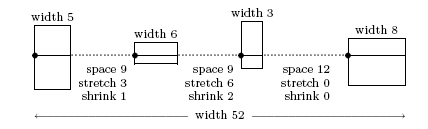
\includegraphics[width=0.9\linewidth]{./images/glue.png}
  \caption{Glue in \TeX}
  \label{fig:glue}
\end{figure}


\section{How to specify glue}

The usual way to specify \textit{glue} to \tex is
$<dimen>< plus~dimen><minus~dimen>$

where the plus and minus are optional and assumed to be zero if not
present; plus\index{glue!plus} introduces the amount of stretchability\index{glue!stretchability}, minus introduces the amount of shrinkability \index{glue!shrinkability}. 

For example, Appendix B of the TexBook defines \cs{medskip} to be an abbreviation for
|\vskip6pt plus2pt minus2p|. The normal-space component of glue must always be
given as an explicit dimen, even when it is zero. The ability of \TeX to stretch and shrink this glue has given it its beautiful looks. Strangely enough, although the algorithm is public it has not been used widely in other software.



\subsection{hfil and hfill}

{\obeylines
{This text will be flush left.\hfil}
{\hfil This text will be flush right.}
{\hfil This text will be centered.\hfil}
{Some text flush left\hfil and some flush right.}
{Alpha\hfil centered between Alpha and Omega\hfil Omega}
{Five\hfil words\hfil equally\hfil spaced\hfil out.}
}

Consider the following definitions:

\begin{verbatim}
\def\centerlinea#1{\hfil#1\hfill}
\def\centerlineb#1{\hfill#1\hfill}
\def\centerlinec#1{\hss#1\hss}
We define quickly a \cs{lineX}\footnote{Strange but my \LaTeX\ distribution has not got on. (This definition is from \texttt{plain.sty}}

\def\lineX{\hbox to\hsize}
\def\lineX{\hbox to\hsize}
\def\centerlinea#1{\hfil#1\hfil}
\def\centerlineb#1{\hfill#1\hfill}
\def\centerlinec#1{\hss#1\hss}

\lineX{\centerlinea{\test}}
\lineX{\centerlineb{\test}}
\lineX{\centerlinec{\test}}
\centerline{\test}
\begin{center}\test\end{center}

\end{verbatim}


\section{Specifying glue amounts}

\tex glue is specified as a fixed dimension, and optionally, with a plus and
or minus dimension. Along with \cs{dimen} registers, TEX has glue registers,
called \cs{skip0} through \cs{skip255}. Here is how you can save glue settings in
\tex registers, and ask \tex to display the contents of one of them:

\begin{teX}
\skip1 = 10pt
\skip2 = 10pt plus 3pt
\skip3 = 10pt minus 2pt
\skip4 = 10dd plus 3dd minus 2dd
\the \skip4
\end{teX}


\texttt{> 10.70007pt plus 3.21002pt minus 2.14001pt}

The four sample glue settings store, respectively, {\em fixed glue}, {\em  stretchable
glue}, {\em shrinkable glue}, and {\em flexible glue}  that can both stretch and shrink,
but only up to a specified amount. Interword and intersentence spaces are
generally defined with glue like this, so that if more stretch or shrink of  a
re underfull (too little text to fill the line), or overfull (too much text in the
line).



\section{Overfull lines}

Although overfull lines are reported in the \tex log file, they can be hard
to find in the typeset document if they only stick out a little. To make
them highly visible while you are fine tuning your final document, assign
the variable \cs{overfullrule} a nonzero dimension, such as 2 cm. \tex then
displays a solid black box, called a \emph{rule}, of that width in the right margin
on each line that is overfull. Using the \docpkg{microtype} package one can adjust the parameters to minimize this.

To make the rules disappear, simply remove it,
or comment out, the assignment, or reset its value to 0 pt. 

Just as you can assign dimension registers to count registers to convert
from points to scaled points, you can assign skip registers to dimension and
count registers to discard the flexible parts:


\begin{teX}
\skip1 = 10pt plus 3pt minus 2pt
\the\skip1
 \dimen1 = \skip1
\the \dimen1
\count1 = \skip1
\the \count1
\end{teX}




\section{More on glue in boxes}

Besides normal glue with fixed amounts of stretch and shrink, \tex also has
two kinds of glue that are \emph{infinitely} stretchable and shrinkable: \cs{hfil} and
\cs{hfill} in horizontal mode, and \cs{vfil} and \cs{vfill} in vertical mode. Notice that there two versions
of the commands, the one ends with one ell and the second one with two. The
two-ell forms are more flexible than the one-ell forms.

The boxes and glue model is powerful, and \tex's author, Donald Knuth,
has written that he views it as the key idea that he discovered when he
first sat down in 1977--1978 to design a computer program for typesetting.
For example, to set something flush left, put infinitely-stretchable glue on
its right. To set it flush right, put the glue on the left. For centered material,
put the glue on both sides. Here are four examples, with vertical
bars marking the ends of the horizontal box (boxes have no visible frames,
although it is possible to write \tex commands to give them such outlines,
and we use that feature shortly):





\section{Horizontal and vertical boxes}


\begin{docCommand}{hbox}{\marg{material}}
\end{docCommand}

Like their dimensions \TeX's boxes are not what one thinks when thinking of boxes. TeX's boxes come in basically two flavours, horizontal boxes and vertical boxes. An \cs{hbox} is created by the command \refCom{hbox}\marg{material}. It has the following properties:

\begin{enumerate}
\item The material is placed from left to right and it becomes a \textit{horizontal list}.\index{horizontal list}
\item The box \textbf{cannot be broken across lines}; it is an indivisible unit.
\end{enumerate}

An |hbox| can contain, characters, horizontal glue, horizontal leaders or other boxes. While in many cases these other boxes can be other |\hbox|es, |\vbox| can be used.


The \refCom{hbox} command has another form |\hbox to <dimen>|\marg{material}. This
creates a box whose width is the given (dimen). Thus |\hbox to lcm{<material>}|
will create a 1 inch wide box \hbox to 1cm{text}. However, we have to supply exactly 1 cm worth of
material to fill up the box; otherwise we end up with an error message. It is best
to consider this form of the command as a promise; we promise '\tex that we will
supply just enough material to fill up the box. 

We can place other hboxes in an hbox. By adding glue we can then move them left or right

\begin{texexample}{hbox and glue}{ex:hbox}
\bgroup
\Huge
\hbox to \textwidth{\hfill \hbox{\EOofficerI}\hbox{\EOofficerII}\hbox{\EOofficerIII} \hfill}

\hbox to \textwidth{\hfill \hbox{\EOofficerI}\hbox{\EOofficerII}\hbox{\EOofficerIII} \hfil}

\hbox to \textwidth{\hfill \hbox{\EOofficerI}\hfill \hbox{\EOofficerII}\hfill \hbox{\EOofficerIII} \hfill}
\egroup
\end{texexample}

The last command that affects the shape of an |\hbox| is 'spread(dimen)', which
spreads the box beyond its natural width. An |\hbox spread12pt|{(material)}
makes the box 12 points wider than its natural size. If the material in the box has
no flexibility, it cannot spread to fill up the additional space, resulting in an underfull
box. This is why 'spread' is normally used with flexible glues.

\begin{texexample}{hbox and glue}{ex:hbox}
\bgroup
\LARGE
\hbox to 5cm{\EOofficerI\EOofficerII\hfill\EOofficerIII}

\hbox spread5cm{\hfill\EOofficerI\hfill\EOofficerII\hfil\EOofficerIII}

\hbox spread9cm{\EOofficerI\hfill\EOofficerII\hfil\hfil\EOofficerIII}

\hbox spread7cm{\EOofficerI\hfill\EOofficerII\hfil\hfil\EOofficerIII} 


\makeatletter
\hb@xt@ 5cm {\EOofficerI\EOofficerII\hfill\EOofficerIII}
\makeatother
\egroup
\end{texexample}



Boxes can be moved up or down using |\raise| or |\lower|. Each of these primitives is followed by a dimension indicating how far the box can be lowered or raised.

Other material that can go in an hbox, is \textbf{vertical rules}. 

\subsection{The null macro}

The |\null| macro is defined both in Plain as well as LaTeX and generates an empty box. Its definition is:

\begin{teXXX}
\def\null{\hbox{}}
\end{teXXX}


\fbox{\hbox{This is a test}}

{
\fbox{\hsize=5cm
A test of a box at the end of a 2.0 inch line\par}

\fbox{\hsize=5.0cm in A test of a box at the end of a \hbox to 2cm{2.0 cm} line\par}

}

What happens when we have more than two boxes on a line? TeX will stuck them one under another. If they are enclosed within another hbox they will be inlined.



\begin{texexample}{}{}
\hbox to 1cm {A} \hbox to 1cm {B}

If we however, put them together in another |\hbox|, we get:

\hbox{\hbox to 1cm {A} \hbox to 1cm{B}}
\end{texexample}




An |\hbox| does not imply horizontal mode, so an attempt to start a paragraph with a box, for
instance
|\hbox to 0cm{\hss$\bullet$\hskip1em}Text ...|

will make the text following the box wind up one line below the box. It is necessary to switch
to horizontal mode explicitly, using for instance |\noindent| or |\leavevmode|. The latter is defined
using |\unhbox|, which is a horizontal command.


\begin{texexample}{}{}
\hbox to 0cm{\hss$\bullet$\hskip1em} Text ...


\leavevmode\hbox to 0cm{\hss$\bullet$\hskip1em} Text ...

\end{texexample}




\section{Kerning}


Using the command \cs{kern}, we can move boxes either left or right. Kerning is extensively used to build internal commands and we discuss it in more detail under the chapter for fonts.

\begin{docCommand}{kern}{\meta{dimen}}
A |\kern| is similar to glue [75], with two differences: (1) |\kern| is rigid; (2)
|\kern| specifies a point where a line, or a page, should not be broken. Since a box is
indivisible anyway, |\kern| is used in a box to indicate rigid spacing. It is interesting
to note that the same command, |\kern|, indicates horizontal spacing when used in
an |\hbox| and indicates vertical spacing when used in a |\vbox|.
\end{docCommand}
Consider two horizontal boxes, holding the letters A and V:
As you can observe, the letters AB are a bit afar, from what would be a visually pleasant arrangement, we can kern them as follows:
\medskip

\begin{teXXX}
\hbox{\Huge AV A\kern-5ptV}
\end{teXXX}
\medskip

Note that hbox, does not produce a frame. I~have used a frame |\fbox|, which will cover a bit later as well as scaled the image by 2, in order to see the effects more clearly.


\drawfontbox{\upshape\Huge FJord F\kern-5pt Jorp}





\noindent\begin{tabular}{ll}
|\hbox{\kern4pt A\kern8pt B\kern8pt C\kern4pt}| & \fbox{\hbox{\kern4pt A\kern8pt B\kern8pt C\kern4pt}} \\
~ &\\
\midrule
|\hbox{\kern4pt\raise1pt\hbox{A}|  & \fbox{\hbox{\kern4pt\raise1pt\hbox{A} \kern8pt BC\kern8pt\lower6pt\hbox{D} \kern4pt} \kern8pt BC\kern8pt\lower6pt\hbox{D}\kern4pt} \\
|\kern8pt BC|                      &\\
|\kern8pt\lower6pt\hbox{D}|        &\\
|\kern4pt}|                        &\\ 
|\kern8pt BC|                      &\\ 
|\kern8pt\lower6pt\hbox{D}|        &\\
|\kern4pt}| &\\
\midrule
\end{tabular}


\vbox{
\noindent\rule{\linewidth}{0.4pt}
\begin{minipage}{4.5cm}
 \begin{teXX}
\fbox{\hbox{\kern4pt A\kern8pt 
      B\kern8pt C\kern4pt}}
\end{teXX}
\end{minipage}
\hfill\hfill
\begin{minipage}{3cm}
\hfill\hfill\fbox{\hbox{\kern4pt A\kern8pt 
      B\kern8pt C\kern4pt}}
\end{minipage}

\medskip
\noindent\rule{\linewidth}{0.4pt}
}

Notice that an |\hbox| is constructed by setting its components side by side so that their \textit{baselines} are aligned. When \cs{raise}, \cs{lower} are used the baselines are no longer aligned. In such a case the baseline of the box is defined as the baseline shared by the components before any vertical movements. In the example above the box now has a depth, as a result of lowering |D|.


\vbox{
\noindent\rule{\linewidth}{0.4pt}
\begin{minipage}{4.5cm}
\begin{teXXX}
\hbox{\kern4pt\raise1pt\hbox{A} 
  \kern8pt BC\kern8pt
  \lower6pt\hbox{D} 
  \kern4pt} 
\end{teXXX}
\end{minipage}
\hfill
\begin{minipage}{3cm}
\fbox{\hbox{\kern4pt\raise1pt\hbox{A} 
\kern8pt BC\kern8pt\lower6pt\hbox{D} \kern4pt}}
\end{minipage}

\medskip
\noindent\rule{\linewidth}{0.4pt}
}



\noindent\textbf{Vertical boxes.}\quad A vertical box is build in a similar manner to that of a horizontal list, except it is composed of material in the \textit{vertical list}.
When horizontal boxes are added in the list, they are stuck on top of each other as shown in the example below. 
\medskip

\bgroup
\parindent0pt
\fbox{\vbox{\hsize=3cm\fbox{\hbox{ABCDEFGH}} \fbox{\hbox{AB}}}}
\egroup


\begin{docCommand}{vbox}{ to \meta{dimen}\marg{\meta{material}}}
Typesets a box in vertical mode.
\end{docCommand}

It is important to remember the two main differences between hboxes and vboxes. An hbox will expand to hold its material. If it need be it will overfill the line and produce an overful warning. A vbox will expand to hold its material. It is perfectly normal for a vbox to hold paragraphs, as shown. This is not possible with an hbox. However, the common pattern is for an |\hbox| to contain a |vbox| .

\begin{texexample}{hbox/vbox example}{ex:vbox}
\noindent\fbox{\vbox{\lorem\par\lorem\par}}

\hbox to \linewidth{\vbox{\lorem\par\lorem\par}}
\end{texexample}


\begin{docCommand}{hsize}{\meta{dimen}}
 Controls the width of text in a |vbox|.
\end{docCommand}

\noindent\textbf{Controlling the size of a vbox.}\quad What controls the size, is the containing environment. This in TeX, is specified using |\hsize|. In LaTeX this is controlled by an enclosing environment, maybe a minipage (which is build this way) or one of the page width parameters.


\begingroup
\parindent0pt
\fboxsep5pt
\hsize=3.9cm\footnotesize
\hfil\fbox{\vbox{\RaggedRight\lorem\par}} 
\hfil\fbox{\vbox{\RaggedRight\lorem\par}}
\hfil\fbox{\vbox{\RaggedRight\lorem\par}}\hfill
\endgroup
\captionof{figure}{Output to demonstrate the use of vboxes.}



The code to typest the boxes shown above follows:
\medskip
\emphasis{hsize}
\begin{teXXX}
\bgroup
\parindent0pt
\hsize=3.3cm\footnotesize
\hfil\fbox{\vbox{\lorem\par}} 
\hfil\fbox{\vbox{\lorem\par}}
\hfil\fbox{\vbox{\lorem\par}}
\hfill
\egroup
\end{teXXX}


Note, the use of \docAuxCommand{hsize}. We define the font size as |\footnotesize|. We have done this in order not to have overfull boxes--Latin words don't have a full set of hyphenation patterns in \latex. The macro |\lorem|, we have defined internally for this document. We place the code in a group in order not to affect the rest of the document.



\clearpage

\noindent\textbf{Vertical centering}\quad can be achieved by applying vertical infinite glue \cs{vfill}. In the example that follows, first we place two letters in individual |\hboxes| and we enclose them in a vbox. We apply |\vfill| both on top and at bottom.

\emphasis{\vfill}

\vbox{
\noindent\rule{\linewidth}{0.4pt}
\begin{minipage}{5cm}
\begin{teX}
\fbox{\vbox to 0.9cm{\vfil\hbox{M}\nointerlineskip\hbox{i}\vfil}} 
\end{teX}
\end{minipage}
\hfill
\begin{minipage}{3cm}
\hfill\fbox{\vbox to 0.9cm{\vfil\hbox{M}\nointerlineskip\hbox{i}\vfil}}\hfill\hfill 
\end{minipage}

\medskip
\noindent\rule{\linewidth}{0.4pt}
}



A |\vbox| can be combined with text and may appear anywhere within a paragraph. The baseline of the box will be aligned with the baseline of the current line.


\vbox{%
\noindent\rule{\linewidth}{0.4pt}}

\begin{teX}
A vbox can be placed within a paragraph \fbox{\vbox to 0.6cm{\vfil\hbox{M}\nointerlineskip\hbox{i}\vfil}} as shown here.


\hfill

A vbox can be placed within a paragraph \fbox{\vbox to 0.6cm{\vfil\hbox{M}
  \nointerlineskip\hbox{i}\vfil}} as shown here.

\end{teX}

\medskip
\noindent\rule{\linewidth}{0.4pt}






\noindent\textbf{Top alignment.}\quad\cs{vtop} is similar to a |\vbox|. The depth of this box is zero, since both A and B are capital letters. The width of this box is |\hsize|, since it contains text. 


\begin{codeexample}[]
\vtop{\hbox{A} \hbox{B}}
\end{codeexample}






Centering a picture in a box, both vertically and horizontally can be achieved using the methods we described so far.


\emphasis{hfill,hbox}
\begin{texexample}{}{}
     \fbox{%
          \vtop{\medskip
                    \hfill
                      \hbox{\includegraphics[width=1.5cm]{./images/amato.jpg}}%
                    \hfill 
                   \medskip%
                }%
      }%
\end{texexample}

\begin{texexample}{}{}
    \fbox{%
          \vtop{\medskip
                    \hfill
                      \hbox{\includegraphics[width=1.5cm]{./images/amato.jpg}}%
                      \hbox{\includegraphics[width=1.5cm]{./images/amato.jpg}}%
                      \hbox{\includegraphics[width=1.5cm]{./images/amato.jpg}}%    
                    \hfill 
                   \medskip%
                }%
      }%
\end{texexample}

Study the example a bit more carefully, as we have said earlier on that \cs{hbox}'es are stacked vertically, the reason why in the above example they are next to each other is that they are in an
\cs{fbox} which in turn is an \cs{hbox}  that can draw  frame around the box and is defined in the
\latex2e kernel.

So if we had only three images in hboxes we will get:

\begin{texexample}{Three Images Lined}{}
%\leavevmode
%\parindent30pt
\hbox{\includegraphics[width=1.5cm]{./images/amato.jpg}}%
\hbox{\includegraphics[width=1.5cm]{./images/amato.jpg}}%
\hbox{\includegraphics[width=1.5cm]{./images/amato.jpg}}%
\end{texexample}

An hbox does not start a paragraph. If we started a paragraph the behaviour will be different.

\begin{texexample}{Three Images Lined}{}
.\hbox{\includegraphics[width=1.5cm]{./images/amato.jpg}}%
\hbox{\includegraphics[width=1.5cm]{./images/amato.jpg}}%
\hbox{\includegraphics[width=1.5cm]{./images/amato.jpg}}%
\end{texexample}

If you notice carefully, we have started the paragraph by inserting a `.' before the first |\hbox|, an alternative way is to 
use |\leavevmode|. The effect of this command is to leave vertical mode, and to enter horizontal mode. Thus, if the mode is vmode (typically, outside any paragraph), a new paragraph is started. This paragraph may be flushed left, flushed right. 

\begin{texexample}{Three Images Lined}{}
\leavevmode
\hbox{\includegraphics[width=1.5cm]{./images/amato.jpg}}%
\hbox{\includegraphics[width=1.5cm]{./images/amato.jpg}}%
\hbox{\includegraphics[width=1.5cm]{./images/amato.jpg}}%

\meaning\leavevmode
\end{texexample}

The macro |\leavevmode| as its name implies forces \tex to leave vertical mode and enter horizontal mode. In this case the photos are just treated by \tex similarly to any character and tehy are typeset next to each other. 

\begin{docCommand}{kern}{}
If we wanted to add a bit of space between the horizontal images, we could use \cs{kern}
Kern again. This is from the book TeX for The Impatient page 157. You can use kern in math mode, but you cannot use the \texttt{mu} units. If you want to use \texttt{mu} units use \cs{mkern} instead.
\end{docCommand}

\emphasize{kern}
\begin{texexample}{}{}
\leavevmode
\hbox{\includegraphics[width=1.5cm]{./images/amato.jpg}}\kern10pt
\hbox{\includegraphics[width=1.5cm]{./images/amato.jpg}}\kern10pt
\hbox{\includegraphics[width=1.5cm]{./images/amato.jpg}}%
\end{texexample}

One needs to be careful as to where you issue |\leavevmode|. If it is in the middle of a paragraph it will have no effect.
\emphasize{This,is,some,text}
\begin{texexample}{Example with leavevmode}{}
This is some text
\leavevmode
\hbox{\includegraphics[width=1.5cm]{botticelli-34.jpg}}\kern10pt
\hbox{\includegraphics[width=1.5cm]{botticelli-34.jpg}}\kern10pt
\hbox{\includegraphics[width=1.5cm]{images/botticelli-34.jpg}}%
\end{texexample}

A very common way in \latex2e is to issue a |\par| command before |\leavevmode| to avoid this problem. Another way is to use
one of the |\ifvmode| or |\ifhmode| and act accordingly. We now fix our example and get what we want. 

\emphasize{par}
\begin{texexample}{}{}
This is some text
\par\leavevmode
\hbox{\includegraphics[width=1.5cm]{botticelli-34.jpg}}\kern10pt
\hbox{\includegraphics[width=1.5cm]{botticelli-34.jpg}}\kern10pt
\hbox{\includegraphics[width=1.5cm]{images/botticelli-34.jpg}}%
\end{texexample}

\begin{texexample}{}{}
   \HHUGE
   \fboxsep=0pt
   \fbox{%
          \vtop{\medskip
                    \hfill
                       \hbox{ H\kern10pt i\kern10pt j}%    
                       \hbox{ A\kern10pt C\kern10pt j}%
                    \hfill 
                   \medskip%
                }%
   }%
\end{texexample}

This example shows how letters are typeset and you can see that they are aligned at the baseline. They are no different than the eimage example that we have shown earlier, except we don't need the boxes.

\medskip

\vbox{
\noindent\rule{\linewidth}{0.4pt}
\begin{minipage}{4.9cm}
\begin{teX}
\centerline{$\Downarrow$}\kern 3pt%
\centerline{$\Longrightarrow$\kern 6pt% horizontal kern
  \textit{A note about kern}\kern 6pt
    $\Longleftarrow$}
\kern 3pt
\centerline{$\Uparrow$}  
\end{teX}
\end{minipage}
\hspace{0.3cm}
\begin{minipage}{4.5cm}
\centerline{$\Downarrow$}\kern 3pt%
\centerline{$\Longrightarrow$\kern 6pt% horizontal kern
  \textit{A note about kern}\kern 6pt
    $\Longleftarrow$}
\kern 3pt
\centerline{$\Uparrow$}
\end{minipage}

\medskip
\noindent\rule{\linewidth}{0.4pt}
}
\medskip

To make a point again, |\vbox| lines boxes at their bottom while, |\vtop| lines them at their top.

\medskip

\vbox{
\noindent\rule{\linewidth}{0.4pt}
\begin{minipage}{4.9cm}
\begin{teX}
 \hbox{\hsize=2cm \raggedright
\vbox to 0.5in{\hrule This box is .5in deep. \vfil\hrule}
\qquad
\vbox to 0.75in{\hrule This box is .75in deep. \vfil\hrule}
\qquad
\end{teX}
\end{minipage}
\hspace{0.3cm}
\begin{minipage}{4.5cm}
\hbox{\hsize=2cm \raggedright
\vbox to 0.5in{\hrule This box is .5in deep. \vfil\hrule}
\qquad
\vbox to 0.75in{\hrule This box is .75in deep. \vfil\hrule}
\qquad}
\end{minipage}

\medskip
\noindent\rule{\linewidth}{0.4pt}
}

\medskip


Trying the same with vtop

\medskip

\vbox{
\noindent\rule{\linewidth}{0.4pt}
\begin{minipage}{4.9cm}
\begin{teX}
 \hbox{\hsize=2cm \raggedright
\vbox to 0.5in{\hrule This box is .5in deep. \vfil\hrule}
\qquad
\vbox to 0.75in{\hrule This box is .75in deep. \vfil\hrule}
\qquad
\end{teX}
\end{minipage}
\hspace{0.3cm}
\begin{minipage}{4.5cm}
\hbox{\hsize=2cm \raggedright
\vtop to 0.5in{\hrule \smallskip This box is .5in deep. \vfil\hrule}
\qquad
\vtop to 0.75in{\hrule \smallskip This box is .75in deep. \vfil\hrule}
\qquad}

\hbox{\hsize=2cm \raggedright
\vbox to 0.5in{\hrule \smallskip This box is .5in deep. \vfil\hrule}
\qquad
\vbox to 0.75in{\hrule \smallskip This box is .75in deep. \vfil\hrule}
\qquad}
\end{minipage}

\medskip
\noindent\rule{\linewidth}{0.4pt}
}

\medskip

There are some other special macros defined by Plain TeX that we will only touch briefly here. One of them is \cs{underbar}{\index{Plain!\textbackslash underbar}.
The macro puts its argument into an hbox and underlines it.

\medskip

\vbox{
\noindent\rule{\linewidth}{0.4pt}
\begin{minipage}{4.9cm}
\begin{teX}
 \underbar{1,000,788.22}
\end{teX}
\end{minipage}
\hspace{0.4cm}
\begin{minipage}{4.0cm}
\medskip
\hfill\hfill{}\hspace*{1em}a1,000,700.22 \hfill

\smallskip

\hfill\[\underbar 1,000,788.22 \]\hfill
\end{minipage}

\medskip
\noindent\rule{\linewidth}{0.4pt}
}

\medskip


The \cs{everyvbox} command inserts a series of tokens at the beginning of every |\vbox|.


\medskip

\vbox{
\noindent\rule{\linewidth}{0.4pt}
\begin{minipage}{4.9cm}
\begin{teX}
 \everyvbox{$\bullet$}...
\end{teX}
\end{minipage}
\hspace{0.4cm}
\begin{minipage}{4.0cm}
\begingroup% Without this group, there are tons of problems!
   \everyvbox{$\bullet$}
   \global\setbox1=\vbox{This is a paragraph without an initial indent. It is   \the\hsize\ long lines.}
   \global\setbox2=\vtop{\copy1}
\endgroup
 \hbox{\box1} 

 \hbox{\box2}
\end{minipage}

\medskip
\noindent\rule{\linewidth}{0.4pt}
}

\medskip
Knuth in the TexBook Chapter 24, has some short description of the every commands. The `everyhbox` inserts a token list just before as its name implies a horizontal box.

Here is a short example. We define a `oneLineBox`, which is simply an hbox with some text and we add spread to spread the line. Using |\everybox| we add the letter \textbf{a} in each horizontal box. 


\tex considers the box overfull if the excess width of the box is larger than \cs{hfuzz} or \cs{hbadness} is less than 100. If I change  the badness to hbadness, I get 1000.

\medskip

\vbox{
\noindent\rule{\linewidth}{0.4pt}
\begin{minipage}{10.0cm}
\begin{teX}
 \begingroup
     \everyhbox{a}
     \def\oneLineBox#1#2%
     {%
          \hfuzz=0pt
          \overfullrule=0.25pt
          \setbox0=\hbox spread#2{#1}%
          \setbox1=\hbox{\the\badness}% 
          \setbox2=\hbox to 4.5cm{\box0\hfil\box1}%
          \box2
     }
     \oneLineBox{Badness of line }{-1em}
     \oneLineBox{Badness of line }{-0.54em}
     \oneLineBox{Badness of line }{-0.4em}
     \oneLineBox{Badness of line }{0em}
     \oneLineBox{Badness of line }{1em}
     \oneLineBox{Badness of line }{2em}
     \oneLineBox{Badness of line }{3em}
 \endgroup
\end{teX}
\end{minipage}


\begin{minipage}{10.0cm}
\begingroup
     \everyhbox{a}
     \def\oneLineBox#1#2%
     {%
          \hfuzz=0pt
          \overfullrule=0.25pt
          \setbox0=\hbox spread#2{#1}%
          \setbox1=\hbox{\the\badness}% 
          \setbox2=\hbox to 4.5cm{\box0\hfil\box1}%
          \box2
     }
     \oneLineBox{Badness of line }{-1em}
     \oneLineBox{Badness of line }{-0.54em}
     \oneLineBox{Badness of line }{-0.4em}
     \oneLineBox{Badness of line }{0em}
     \oneLineBox{Badness of line }{1em}
     \oneLineBox{Badness of line }{2em}
     \oneLineBox{Badness of line }{3em}
 \endgroup
\end{minipage}

\medskip
\noindent\rule{\linewidth}{0.4pt}
}

\medskip










\parindent1em




\section{More features of horizontal boxes}

Characters in the Latin alphabet have different shapes, and in most typefaces,
different widths. The letters \texttt{d f h k l t} have ascenders, making them
higher than the vowels \texttt{a e o u}, while the letters \texttt{f g j p q y} have descenders,
giving them added depth below the vowels. Similarly, an \texttt{m} is wider than
an \texttt{i}. 

\drawfontbox{(fjord)}

When \tex makes a normal horizontal box, the box width is the sum
of the widths of the characters, and the fixed parts of any glue, contained
in it. Shrink and stretch components of glue are discarded for the width
calculation. The box also has both a height above the baseline, the invisible
line on which the characters rest, and a depth below the baseline. The
depth is zero if there are no objects with descenders. The height and depth
are chosen from the largest vertical extents of the contained objects.

If you look carefully at typeset material, you will observe that, in most
typefaces, parentheses, brackets, and braces have both descenders and ascenders,
and the typeface designer usually makes their extents the maximum
among all of the characters in the design. This sample text shows
document: ( h g ) [ k j ] { l p }.

You can force TEX to choose a larger height and depth than normal when
you write a command for a horizontal box by ensuring that it has suitable
contents, such as an invisible vertical rule of zero width. The command

\verb+\hbox to 50pt {\vrule height 20pt depth 10pt width 0pt \it stuff}+

produces a box whose (invisible) outline looks like this: 

\hbox to 50pt {\vrule height 20pt depth 10pt width 0pt \it Great}

\drawfontbox{\kern 5pt\vrule height20pt depth 10pt width 1pt fjord}

The
three extents of the vertical rule can appear in any order, and any convenient
units.

In order to see the otherwise-invisible box edges in that example, we
used the \latex  built-in command \cs{fbox} to create a frame, and we eliminated
the default margin inside the frame by setting \cs{fboxsep = 0pt}. Plain \tex
does not have the \cs{fbox} command, but The TEXbook shows how to make
something like it on pp. 223 and 321.

One particular zero-width vertical rule is convenient for ensuring that
separate boxes all get the same height and depth. It has the height and
depth of parentheses in the normal prose font, and is given the macro name \refCom{strut}.
Its definition in the plain.tex file of macro definitions is roughly
equivalent to this:

\begin{docCommand}{strut}{}
\end{docCommand}

\begin{teX}
  \def \strut {\vrule height 8.5pt depth 3.5pt width 0pt}
\end{teX}

We insert a |\vrule| at the figure on the left below with a height of 20pt and a depth of 10pt. You can observe the difference on the right box, without the |\vrule|. The \textit{strut} is the blue line, which we gave a width of one point to make it visible. Real life struts, would have a width of 0pt and will not be visible. 

\drawfontbox{\kern5pt{\color{blue}\vrule height20pt depth 10pt width 1pt} fjord}
\drawfontbox{fjord}



\section{Horizontal alignment of boxes in TEX}
\fboxsep0.4pt

When horizontal boxes are set together, they are treated as separate words,
and therefore spaced accordingly. The input
\verb+ \fbox{one} \fbox{two} \fbox{three} \fbox{four}  +
produces  \fbox{one} \fbox{two} \fbox{three} \fbox{four}. As the example shows, we can put spaces
between them, or run them together so that they fit tightly.


\section{Vertical boxes in TEX}


\begin{minipage}{2.0in}
\begin{verbatim}
\noindent
\fbox{%
  \it
  \hbox to 80pt{%
     \parindent = 0pt
     \vbox to 30pt {%
         left text
         \vfil
         more left text%
     }%
  }%
}%
\end{verbatim}
\end{minipage}


%\noindent
\fbox{%
  \it
  \hbox to 80pt{%
     \parindent = 0pt
     \vbox to 30pt {%
         left text
         \vfil
         more left text%
     }%
  }%
}%

Firstly we use a noindent to ensure that the box is not indented. If you comment the\cs{fbox} out, you can see that the right amount of space has been left in the paragraph above.

\mbox{}
 
\noindent
\fbox{%
\it
\hbox to 80pt{%
\parindent = 0pt
\hsize = 80pt
\vbox to 30pt {\hfill right text
\vfil
\hfill more right text}
}%
}%



\noindent
\fbox{%
\it
\hbox to 80pt{%
\parindent = 0pt
\hsize = 80pt
\vbox to 30pt {\hfil center text
\vfil
 more center text \hfil}
}%
}%

We can aslo center the text for both lines, by modifying the code slightly.
\begin{teX}
\noindent
\fbox{%
\it \hbox to 80pt{
   \parindent = 0pt
   \hsize = 80pt
   \vbox to 30pt {
   center text \hfill
    \vfil
    \hfil more center text}
   }%
}%
\end{teX}


\noindent
\fbox{%
\it
\hbox to 80pt{%
\parindent = 0pt
\hsize = 80pt
\vbox to 30pt {\hfil center text
\vfil
\hfil more center text}
}%
}%



\chapter{Boxes with \protect\LaTeXe}

The \tex primitive commands have been abstracted by \latexe into more user friendly commands that are easier to use. One other reason for using these \LaTeX\ commands is that they are ``color safe''. Later on we will see other possibilities given by the \pkgname{color} or \pkgname{xcolor} package for drawing colored boxes, but we want to recall that the code for |\makebox| and the like has already a protection mechanism for colors, which the primitive commands do not have. \latexe also provides boxes that are self-aware of the width of their contents. For example |\fbox| will frame its contents in an |\hbox|. This simple task is very convoluted to achieve using basic \tex commands. 

\begin{docCommand}{framebox} {\marg{dim}}
One useful box command provided by \latex2e is \cmd{\framebox}. This command builds a box with any material you want to provide it with. The contents of this box are unbreakable, and as far as \tex is concerned it is treated the same way as it would treat a letter. 
\end{docCommand}

\begin{docCommand}{fboxsep}{\marg{dim}}
\end{docCommand}
\begin{docCommand}{fboxrule}{\marg{dim}}
Two associated lengths control the width of the rule and the space around the contents. We can change their default value by using |\setlength{\fboxsep}{0pt}| or just simply |\fboxsep=0pt| or even |\fboxsep0pt|. 
\end{docCommand}


Another interesting property is this: \emph{the contents of a box need not lie inside it}. You may have
noticed that, given the contents as an argument, the
|\framebox| command sets the dimensions of the box
to those of the contents (in reality, to the ``sub-boxes"
that compose the contents). But you can define the
dimensions explicitly as well. For example,

\begin{texexample}{framebox example}{ex:framebox}
|\framebox[13em]{Some text}|

\framebox[13em]{Some text}

\fcolorbox{theblue}{cyan}{Some text}

\end{texexample}

The box as is shown in the example will not break and it occupies more space than its contents. A second optional command allows us to typeset the contents, left, center or right.

\begin{codeexample}[vbox]
\fboxrule1pt

\framebox[13em][l]{Some text}\par

\framebox[13em][r]{Some text}\par

\framebox[13em][c]{Some text}\par

\framebox[1em][l]{Some text}\par

\framebox[1em][c]{Some text}\par

\framebox[1em][r]{Some text}\par
\end{codeexample}

As you can observe \latexe has abstracted the |\hfill| and similar commands and allows boxes to be constructed with ease. We have started the discussion with |\framebox|, but most practical uses of boxes is when they remain invisible.

\begin{docCommand}{makebox} { \oarg{width}\oarg{position}\marg{contents} } 
 is \latex's box workhorse.
 \end{docCommand}

The |source2e| manual states. If the width is missing, then position is also missing and |obj|  is put in an \cs{hbox} of its natural width. This is true as far as the looks are concerned, but not the behaviour, as you can see
from the following example is not an unqualified \cmd{\hbox} it is an hbox preceded by leavevmode.\footnote{\url{http://tex.stackexchange.com/questions/105585/latex2e-makebox-hbox}} This is of course good practice and brings consistency to the LaTeX kernel. I would recommend that you follow such practices in your own code. 

\begin{texexample}{}{}
\newbox\temp
\savebox\temp{test}
LaTeX

\makebox{test} \mbox{test}

TeX

\hbox{test} \hbox{test}

\indent\hbox{test} \hbox{test}

LaTeX with \cs{leavemode}

\makeatletter
\leavevmode\hbox to \wd\temp{test} \indent\hbox to \wd\temp{test}
\makeatother
\end{texexample}



\latex's analog of a\cs{hbox} is called \cs{mbox}. They are 
much the same thing, but \cs{mbox} is defined to be more widely usable. We have already used \latex's framed companion to \cs{mbox}, \cs{fbox}.

A horizontal box of specified width is provided in \latex with the command
\doccmd{makebox[width][position]\{contents\}}. Bracketed command arguments
in \latex are always optional. 

Here, the width is a \tex dimension,
and defaults to the natural width of the contents if not given. The position
is one of the letters \textbf{l} (flush left) or \textbf{r} (flush right); if it is omitted, the text
is centered in the box. If the specified width is smaller than needed, the
contents protrude from the box, and may overlap surrounding material. If
the specified width is zero, then we have equivalents of the TEX \cs{rlap} and
\cs{llap} commands.


Here are several examples of these three LATEX box commands:

{\obeylines
\mbox{stuff}

\fbox{stuff} 

|\makebox{stuff}|

|\makebox[40pt][l]{stuff}|

|\makebox[40pt][r]{stuff}|

|\makebox[0pt]{stuff}|

|\makebox[0pt][l]{stuff}|

|\makebox[0pt][r]{stuff}|
}



\subsection{Positioning boxes}

To help in positioning boxes within other objects, \latex provides the command
\docAuxCmd{raisebox} to raise and lower boxes:

\begin{teX}
\raisebox{raiselength}[height][depth]{contents}
\end{teX}

A negative first argument lowers the box, where the \cmd{\lowerbox} will lower the box. Here are some examples:

\begin{texexample}{Raising and lowering boxes}{ex:raise}
A \raisebox{10pt}{\fbox{upper}} A
upper
A \raisebox{10pt}{\
fbox{lower}} A
lower
A \fbox{\raisebox{10pt}[25pt]{\fbox{upper}}} A
upper
A \fbox{\raisebox{10pt}[
25pt]{\fbox{lower}}} A
lower
A \fbox{\raisebox{10pt}[25pt][15pt]{\fbox{upper}}} A
upper
A \fbox{\raisebox{10pt}[
25pt][15pt]{\fbox{lower}}} A
lower
\end{texexample}

\section{Paragraph Boxes}

\begin{docCommand}{parbox}{\oarg{position}\oarg{height}\oarg{innerpos}\marg{width}\marg{contents} }
  For longer strings of text, \latex provides the paragraph box \cs{parbox} 
\end{docCommand}


The optional position
is a letter \textbf{b} for alignment of the bottomline with the current baseline,
or \textbf{t} for alignment of the top line with the surrounding baseline. Without

The box can be used as if it were a letter or a word, so we can put it in
the middle of a sentence. The input

This is text \parbox{30pt}{\it and this is boxed text} and
this is more text.

This is text \fbox{\parbox{30pt}{\it and this is boxed text}}
and this is more text.
produces


Flush-right typesetting generally looks bad in narrow columns, so we
can insert a \cs{raggedright} command inside the last argument of the paragraph
box to get output like this:

\begin{texexample}{}{}

\parbox[b][120pt][t]{130pt}{\lorem}%
\hspace{1cm}%
\parbox[b][150pt][t]{130pt}{Only some short line of text here.}%



\parbox[b][120pt][t]{130pt}{\lorem}\hspace{1cm}\parbox[b][120pt][c]{130pt}{Only some short line of text here.}

\end{texexample}


\section{The minipage environment}

Another kind of paragraph box can be obtained in a more general, and
more powerful, way with the \docAuxEnv{minipage} environment:

\emphasis{minipage}
\begin{phdverbatim}
\begin{minipage}[position]{width}
   contents
\end{minipage}   
\end{phdverbatim}


The positioning works just like that for \verb+\parbox+, with alignment letters \textbf{b}
and \textbf{t}, and if they are omitted, a default of vertical centering.
In particular, verbatim text produced with the verb command is illegal
in macro arguments, so it cannot be used with \cs{fbox}, \cs{framebox}, \cs{makebox},
\cs{mbox}, or\cs{ parbox}, but it can be used inside a minipage. The input


\begin{texexample}{}{}
\begin{minipage}{170pt}
This is inline verbatim \verb=\verb|\%{}|=, and this
is a verbatim display:

\begin{verbatim}
#include <stdio.h>
#include <stdlib.h>
int main(void)
{
  printf("Hello, world\n");
  exit (EXIT_SUCCESS);
}
\end{verbatim}
\end{minipage}

\end{texexample}


A minipage can go everywhere and can hold virtually any content.


\section{Scaling and resizing boxes}

\begin{docCommand}{resizebox}{\marg{width}}{\marg{general material}}
Resizes the contents of a box
\end{docCommand}

The command \cs{resizebox}\marg{width}\marg{height}\marg{object} can be used with tabular to specify the height and width of a table. The following example shows how to resize a table to 8cm width while maintaining the original width/height ratio.

\begin{teX}
\resizebox{8cm}{!} {
  \begin{tabular}...
  \end{tabular}
}
\end{teX}

Alternatively you can use \cs{scalebox}{ratio}{object} in the same way but with ratios rather than fixed sizes:

\begin{teX}
\scalebox{0.7}{
  \begin{tabular}...
  \end{tabular}
}
\end{teX}

Both |\resizebox| and |\scalebox| require the \pkg{graphicx}\footfullcite{graphicx} package.
To tweak the space between columns (LaTeX will by default chose very tight columns), one can alter the column separation: |\setlength{\tabcolsep}{5pt}|. The default value is |6pt|.

The scalebox is great if you want to magnify a letter so that you can observe the design closer.

\bigskip
\noindent\begin{tabular}{|c|c|c|c|c|c|}\hline
Kp-Fonts & Kp-\textit{light} & CM & Palatino & Utopia & Times\\\hline\hline
\scalebox{2}{ag713} &
\scalebox{2}{\fontfamily{jkpl}\selectfont 7} &
\scalebox{2}{\fontfamily{lmr}\selectfont 713}  &
\scalebox{2}{\fontfamily{ppl}\selectfont 713}  &
\scalebox{2}{\fontfamily{put}\selectfont 7} &
\scalebox{2}{\fontfamily{ptm}\selectfont \oldstylenums{7}} \\\hline
\end{tabular}


\begin{teX}
\hspace{-6mm}\begin{tabular}{|c|c|c|c|c|c|}\hline
Kp-Fonts & Kp-\textit{light} & CM & Palatino & Utopia & Times\\
\hline\hline
  \scalebox{10}{a} &
  \scalebox{10}{\fontfamily{jkpl}\selectfont a} &
  \scalebox{10}{\fontfamily{lmr}\selectfont a}  &
  \scalebox{10}{\fontfamily{ppl}\selectfont 7}  &
  \scalebox{9.2}{\rule{0pt}{1.25ex}\fontfamily{put}\selectfont a} &
  \scalebox{10}{\fontfamily{ptm}\selectfont a}\\\hline
\end{tabular}
\end{teX}
\bigskip



\section{Glues with Negative and zero dimensions}

A box with a natural size of zero with the right glue amount can become very useful. For example the glue
|0pt plus1fil minus1fil| can stretch to infinity and also shring to minus infinity. Of course in the case of
\tex infinity is \docAuxCommand{maxdimen}. A \tex primitive is defined with this glue \refCom{hss}.

\begin{docCommand}{hss}{}
\end{docCommand}

There is also a corresponding \refCom{vss}.

\begin{docCommand}{vss}{}
\end{docCommand}


These macros place text on a full line either centred or left or right adjusted.

\begin{texexample}{}{}
\makeatletter
368 \def\@@line{\hb@xt@\hsize}
369 \def\leftline#1{\@@line{#1\hss}}
370 \def\rightline#1{\@@line{\hss#1}}
371 \def\centerline#1{\@@line{\hss#1\hss}}
\rlap
\llap
These macros place text to the left or right of the current reference point without
taking up space.
372 \def\rlap#1{\hb@xt@\z@{#1\hss}}
373 \def\llap#1{\hb@xt@\z@{\hss#1}}

$a\mathrel{\rlap{\;/}{=}}b $

{\Huge
\leavevmode
\rlap{Y}L
\rlap{C}\kern2.6pt\lower3.5pt\hbox{,}
}
\makeatother
\end{texexample}

\begin{docCommand}{rlap}{\marg{material}}

\end{docCommand}

Of course neither |llap| or |rlap| start a paragraph, so we need to use a |leavevmode| or one of the other ways to start a paragraph.

\begin{docCommand}{llap}{\marg{material}}
\end{docCommand}


\begin{docCommand}{smash}{\marg{material}}
The |\smash| command typesets the material with a height and depth of zero.
\end{docCommand}

\begin{docCommand}{phantom}{\meta{material}}
\end{docCommand}

\begin{docCommand}{vphantom}{\meta{material}}
\end{docCommand}

\begin{texexample}{Defining smash}{}
\bgroup
\def\smash{%
   \relax % \relax, in case this comes first in \halign
   \ifmmode
   \expandafter\mathpalette\expandafter\mathsm@sh
   \else
    \expandafter\makesm@sh
   \fi}
   
\def\makesm@sh#1{%
   \setbox\z@\hbox{\color@begingroup#1\color@endgroup}\finsm@sh}

\def\mathsm@sh#1#2{%
   \setbox\z@\hbox{$\m@th#1{#2}$}\finsm@sh}

\def\finsm@sh{\ht\z@\z@ \dp\z@\z@ \box\z@}
\egroup

\vbox{\smash {\hbox{A} } \hbox{B}} Test

\end{texexample}

\cxset{geometry units = pt,
       fontbox font=\Huge\upshape}

  


Consider the letters `Q' and `P', shown below. The capital letter `Q' has a depth of 1.72mm, we might wish to smash
it in a two line title block to reduce the line spacing between two consecutive lines. This can be accomplished with the
\refCom{smash} command.

\centerline{\drawfontbox{Q} \drawfontbox{P}}

Smashing it produces the following results.

\centerline{\drawfontbox{\vbox{\smash {\hbox{Q} } \hbox{P}}}  \drawfontbox{\vbox{\hbox{Q}  \hbox{P}}}}  

The command is more useful in math environments and is used extensively both by authors and package developers.

\begin{teXXX}
\def\rightarrowfill{$\m@th\smash-\mkern-7mu%
454 \cleaders\hbox{$\mkern-2mu\smash-\mkern-2mu$}\hfill
455 \mkern-7mu\mathord\rightarrow$}

456 \def\leftarrowfill{$\m@th\mathord\leftarrow\mkern-7mu%
457 \cleaders\hbox{$\mkern-2mu\smash-\mkern-2mu$}\hfill
458 \mkern-7mu\smash-$}
\end{teXXX}

Two further macros can be useful to authors of mathematical documents, \docAuxCommand*{phantom} and \docAuxCommand*{vphantom}. 

When typesetting roots, sometimes there are issues with heights. The following example
from \citetitle{mathmode}\footcite{mathmode} illustrates the point.

\begin{equation}
 \sqrt{a}\,%
 \sqrt{T}\,%
 \sqrt{2\alpha k_{B_1}T^i}\label{eq:root1}
\end{equation}

This can be corrected using \refCom{vphantom}. 

\begin{texexample}{Correcting height issues}{ex:sqrtheights}
\begin{equation}\label{eq:root2}
 \sqrt{a\vphantom{k_{B_1}T^i}}\,%
 \sqrt{T\vphantom{k_{B_1}T^i}}\,%
 \sqrt{2\alpha k_{B_1}T^i}
\end{equation}

\begin{equation}
x = \sqrt[3]{6+\sqrt[3]{6+\sqrt[3]{6+\sqrt[3]{6+\cdots}}}}
\end{equation}
\end{texexample}

Using \pkgname{amsmath} \docAuxCommand{smash} can be used for even better results when
using inline or displayed roots. It must be noted that \cs{smash} in \latexe is defined
without such an optional argument.



\makeatletter
\renewcommand{\smash}[1][tb]{%
\def\mb@t{\ht}\def\mb@b{\dp}\def\mb@tb{\ht\z@\z@\dp}%
\edef\finsm@sh{\csname mb@#1\endcsname\z@\z@ \box\z@}%
\ifmmode \@xp\mathpalette\@xp\mathsm@sh
\else \@xp\makesm@sh
\fi
}
\makeatother
This is a test $\sqrt{\lambda_{ki}}$ and $\smash[tb]{\sqrt{\lambda_{ki}}} $ 
\meaning\smash

\begin{docCommand}{smash}{ \oarg{position}\marg{argument} }
The optional argument for the position can take three values: \textbf{t} keeps the bottom and annihilates the top, \textbf{b} keeps the top and annihilates the bottom and \textbf{tb} which annihilates top and bottom. The latter is the default.
\end{docCommand}

\begin{texexample}{Use of Amsmath smash}{ex:amssmash}
xxx
\fbox{\rule{0.5cm}{2cm}}
\fbox{\rule[-1cm]{0.5cm}{2cm}}
\fbox{\smash{\rule{0.5cm}{2cm}}}
\fbox{\smash{\rule[-1cm]{0.5cm}{2cm}}}
\fbox{\raisebox{0pt}[0pt][0pt]{\rule[-1cm]{0.5cm}{2cm}}}
\fbox{\raisebox{-1cm}[0pt][0pt]{\rule{0.5cm}{2cm}}}
\end{texexample}


\begin{texexample}{The array environment}{ex:array2}
Thus to change $\frac34$ to a decimal divide $4$ into $3$
and we get $.75$ as a result, thus:
\[
\begin{array}{r@{}r@{}}
4 \; & \vline \; 3.00 \\\cline{2-2}
     &            .75
\end{array}
\]
To find the square root of a four-figure number
such as our example calls for, work it out in the
following manner:


\[
\arraycolsep=0em
\begin{array}{cccccccccccc}
\multicolumn{3}{c}{\text{2d pair}} &\qquad&\qquad&
\multicolumn{3}{c}{\text{1st pair}}&\qquad&\qquad&
\multicolumn{2}{c}{\text{square root}}\\
 & \overbrace{\quad}&\ZZZ&&&\ZZZ&\overbrace{\quad}&\ZZZ\\
 & 42 &&&&& 25 &&&&\vline\;65&(answer)\\\cline{11-11}
 & 36 &&&&& \\\cline{2-2}
\multirow{2}{*}{125\:} & \vline\hfill \phantom{Z}6 \hfill&&&&& 25\\
 & \vline\hfill \Zi6 \hfill&&&&& 25\\\cline{2-7}
\end{array}
\]
\end{texexample}

What I provided as an easy mnemonic for the \pkg{phd} I provided macros |\Zi, \ZZ, \ZZZ| as convenience aliases for
|\phantom{Z}| etc.

With graphic programs becoming available, most of the drawing of small complicated boxes, has been overtaken by using
\tikzname and especially its option to overlay a node at a particular point of the page without any impact on the spacing.








%\chapter{LaTeX3 Boxes}

\epigraph{If you go far enough back, your genome connects you with bacteria, butterflies, and barracuda---the great chain of being linked together through DNA.}{---Spencer Wells}

The \pkg{l3box} package, provides numerous commands that deal with boxes. Before you delve in the code you should be familiar with \tex’s concepts of boxes such as \docAuxCommand*{hbox} and \docAuxCommand*{vbox}. The package provides a full repertoire of commands, as well as additional helper functions to reduce the number of commands necessary when storing content in boxes. There is also an additional package for handling the \latexe type |\fbox| and |\makebox| commands, still in experimental stage called \pkgname{xbox}. The latter also is attempting to provide some integration with the \pkgname{xcoffins} package which is an entirely new concept for box manipulation in \latex3. Most of the commands are just syntactic translations of the \latexe macros. 

Do they offer any advantage? I am not too sure if they do at this stage. When it comes to boxes, which is such a fundamental typographic concept users expect much more than these basic commands, however one needs to build up from more basic commands and these have to be re-defined to keep up with the spirit of \latex3.

\section{Storing content in boxes}

\tex’s concept of storing content in boxes is fundamental to any programming effort, where the dimensions of typeset material needs to be determined before further processing.

\subsection{Creating and initializing boxes}
\begin{macro}{\box_new:N, \box_new:c} { \meta{box}}
   Creates a new \meta{box} or raises an error if the name is
   already taken. The declaration is global. The \meta{box} will
   initially be void.
\end{macro}

\begin{texexample}{A new box}{ex:boxnew}
\ExplSyntaxOn
\ttfamily
\token_to_meaning:N \box_new:N\\
\token_to_meaning:N \box
\ExplSyntaxOff
\end{texexample}



Normally three operations are involved. Creating an empty box or using one of the available temporary one, setting the contents in a horizontal or vertical or a combination of both of them, measuring them if necessary 
and then using them.

\begin{texexample}{Store content in a box and use it later}{ex:storebox}
\ExplSyntaxOn
\box_new:N \my_box
\hbox_gset:Nn \my_box {\color{theblue} Some~test.}

\ttfamily
\token_to_meaning:N \hbox_set:Nn
\ExplSyntaxOff
\end{texexample}

Traditionally using \tex the command |\setbox=\hbox{..,}| is used. Note with \latex3 we can use either an |hbox| or |vbox| or variants. Now the above did not typset its contents; for this we need to use the macro |\box_use:N|.

\begin{texexample}{...continued store contents}{}
\ExplSyntaxOn
\box_use:N \my_box
\ExplSyntaxOff
\end{texexample}


\begin{texexample}{Storing content in boxes}{l3box}
\ExplSyntaxOn
\box_new:c {temp_textbox}
\hbox_set_to_wd:cnn { temp_textbox } { 5cm } 
  {
    \tex_hsize:D 5cm
    
    \colorbox{spot!10}{\vbox:n  
       { 
         {\lorem }
       }
       }
  }
\medskip

\leavevmode\vbox{ \box_use:c {temp_textbox  }}\vbox{\box_use:c {temp_textbox  }}\par

\leavevmode\hbox{ \box_use:c {temp_textbox  } \box_use:c {temp_textbox  }}
\medskip

The~box~height~is~\the\box_ht:c {temp_textbox}~and~the~box~width~is~\the\box_wd:c {temp_textbox}.\par
\ExplSyntaxOff  
\end{texexample}


As this is is the \tex primitive |copy| we can use the box as many times as we want.

\begin{texexample}{Measuring the contents}{ex: measure contents}

\ExplSyntaxOn

\box_use:c {temp_textbox}

The~box~height~is~\the\box_ht:c {temp_textbox}~and~the~box~width~is~\the\box_wd:c {temp_textbox}.\par

\box_use:c {temp_textbox}

\ExplSyntaxOff

\tikz\node[draw, fill=spot!20, text width=142.26378pt-10pt, inner sep=5pt, outer sep=0pt, baseline=X.base]{\lorem};
\end{texexample}

The naming schemes are a bit unintuitive but this is inherited from \tex itself. To restrict the |\vbox| you need to set the |\hsize|.  

 \begin{docCommand}{box_move_right:nn}{\docAuxCommand*{box_move_right:nn} \marg{dimexpr} \marg{box function}}
 This function operates in vertical mode, and inserts the
  material specified by the \meta{box function}
  such that its reference point is displaced horizontally by the given
   \meta{dimexpr} from the reference point for typesetting, to the right
   or left as appropriate. The \meta{box function} should be
   a box operation such as |\box_use:N \<box>| or a \enquote{raw}
   box specification such as |\vbox:n { xyz }|.
 \end{docCommand}

 \begin{docCommand}{box_move_up:nn}{\docAuxCommand*{box_move_up:nn} \marg{dimexpr} \marg{box function}}
   This function operates in horizontal mode, and inserts the
   material specified by the \meta{box function}
   such that its reference point is displaced vertical by the given
   \meta{dimexpr} from the reference point for typesetting, up
   or down as appropriate. The \meta{box function} should be
   a box operation such as |\box_use:N \<box>| or a \enquote{raw}
   box specification such as |\vbox:n { xyz }|.
 \end{docCommand}
 
\begin{texexample}{Moving Boxes up or down}{l3boxdown}
\ExplSyntaxOn
\vbox_set:cn{temp_textbox}{abcd}
A \box_move_down:nn{10pt}{\box_use:c { temp_textbox }} 
\ExplSyntaxOff
\end{texexample}

 \section{Measuring and setting box dimensions}

\begin{docCommand}{box_dp:N}{\docAuxCommand*{box_dp:N} \meta{box}}
   Calculates the depth (below the baseline) of the \meta{box}
   in a form suitable for use in a \meta{dimension expression}.
\end{docCommand}

\begin{docCommand}{box_ht:N}{\docAuxCommand*{box_ht:N} \meta{box}}
   Calculates the height (above the baseline) of the \meta{box}
   in a form suitable for use in a \meta{dimension expression}.
  This is the \TeX{} primitive \docAuxCommand*{ht}.
 \end{docCommand}

% \begin{function}{\box_wd:N, \box_wd:c}
%   \begin{syntax}
%     \docAuxCommand*{box_wd:N} \meta{box}
%   \end{syntax}
%   Calculates the width of the \meta{box} in a form
%   suitable for use in a \meta{dimension expression}.
%   \begin{texnote}
%     This is the \TeX{} primitive \tn{wd}.
%   \end{texnote}
% \end{function}

\section{Horizontal Boxes}
\label{l3:hboxes}

So far we have discussed the boxing, unboxing and measuring of box dimensions. In the examples we have used
the \latex3 form of |\hbox| and |\vbox|.  Now time to lose our  beloved |source2e| favoured command \docAuxCommand*{hb@xt@} and friends. 

 \begin{docCommand}{hbox:n}{\docAuxCommand*{hbox:n} \marg{contents}}
   Typesets the \meta{contents} into a horizontal box of line width and then includes this box in the current list for typesetting.
   This is the \TeX{} primitive \docAuxCommand*{hbox}.
 \end{docCommand}

\begin{texexample}{Natural width boxes}{l3:hbox}
\ExplSyntaxOn
\cs_new:Npn \put_image:n #1{
  \par\leavevmode
  \centering
  \hbox:n{
\includegraphics[width=#1\textwidth]{latex3}}
  \par
}
\put_image:n {0.6}
\ExplSyntaxOff
\end{texexample}

\begin{texexample}{Natural width boxes}{l3:hbox}
\ExplSyntaxOn
\hbox:n{
\includegraphics[width=0.8\textwidth]{latex3}}
\ExplSyntaxOff
\end{texexample}

\definecolor{nice}{HTML}{48CCD8}
{\fboxsep3pt \sffamily \Huge \colorbox{nice}{\color{white}TEXT}}

\begin{docCommand}{hbox_to_wd:nn}{\docAuxCommand*{hbox_to_wd:nn} \marg{dimexpr} \marg{contents}}
   Typesets the \meta{contents} into a horizontal box of width
   \meta{dimexpr} and then includes this box in the current list for
   typesetting.
\end{docCommand}

\begin{texexample}{Natural width boxes}{l3:hbox}
\ExplSyntaxOn
\DeclareDocumentCommand\PutImage{o m}{
  \IfNoValueTF{#1}
      {\putimage{#2}}
      {\putimage{#1}{#2}}
}

\noindent\hbox_to_wd:nn{0.3\textwidth}{\includegraphics[width=0.3\textwidth]{amato}}
\hbox_to_wd:nn{0.3\textwidth}{\includegraphics[width=0.3\textwidth]{amato}}
\ExplSyntaxOff

\noindent\hbox to 0.3\textwidth{\includegraphics[width=0.3\textwidth]{amato}}%
\hbox to 0.3\textwidth{\includegraphics[width=0.3\textwidth]{amato}}
\end{texexample}

Having set our goodbyes to |\hb@xt@| we also don’t feel very sorry for not having to type \% to eliminate wandering spaces. As we delve further into the intricacies of \latex3 we can also start appreciating its advantages.

% \begin{function}{\hbox_to_zero:n}
%   \begin{syntax} 
%     \docAuxCommand*{hbox_to_zero:n} \Arg{contents}
%   \end{syntax}
%   Typesets the \meta{contents} into a horizontal box of zero width
%   and then includes this box in the current list for typesetting.
% \end{function}

\section{Vertical Boxes}
The vertical box equivalents to \tex’s |\vbox|, |\vtop| are provided, as well as helper functions to store contents in a box typeset zero width boxes or lap them left, right or center. The commands are mostly syntactic sugar to the primitive commands. 

\begin{docCommand}{vbox:n}{\marg{contents}}
Typesets the \meta{contents} into a vertical box of natural height and includes this box in the current list for typesetting.
\end{docCommand}

\begin{docCommand}{vbox_to_ht:nn}{\marg{dimexpr}\marg{contents}}
Typesets the \meta{contents} into a vertical box of height \meta{dimexpr} and includes this box in the current list for typesetting.
\end{docCommand}

\begin{docCommand}{vbox_to_zero:n}{\marg{contents}}
Typesets the \meta{contents} into a vertical box of zero height and includes this box in the current list for typesetting.
\end{docCommand}

%\tcbset{listing options={
%              firstnumber=10, stepnumber=1, belowskip=0pt, 
%              escapeinside={(*@}{@*)},
%              backgroundcolor=\color{graphicbackground}
%              }}
\begin{texexample}{vboxes in LaTeX3}{l3:boxes}
\ExplSyntaxOn
    \fbox{\vbox:n{\lorem}}\par
    \fbox{\vbox_to_ht:nn {1.5cm}{\lorem}}\par
    \fbox{\vbox_to_zero:n {\lorem}}
\ExplSyntaxOff
\vspace*{1cm}
\end{texexample}

In Example~\ref{l3:boxes} we use \docAuxCommand*{vbox_to_ht:nn} and \docAuxCommand*{vbox_to_zero:n} to set text in two vertical boxes. The first one is typeset in a vertical box of 2cm height, whereas the second one in a box of zero height. The macro
|\fbox| which we discussed earlier in the \latexe boxes chapter, is also available in \latex3 but as part of the still under trial package \pkgname{xbox}.\footnote{To make matters more complicated, the version used in this document has been redefined further!} 



%\tcbset{listing options={
%              firstnumber=last, stepnumber=1, belowskip=0pt, 
%              escapeinside={(*@}{@*)},
%              backgroundcolor=\color{graphicbackground},
%              upquote=true,
%          }}
              
\begin{texexample}{vboxes in LaTeX3}{l3:boxes}
\ExplSyntaxOn
    \fbox{\vbox:n{\lorem}}\par
    \fbox{\vbox_to_ht:nn {1.5cm}{\lorem}}\par
    \fbox{\vbox_to_zero:n {\lorem}}
\ExplSyntaxOff
\vspace*{1cm}
\end{texexample}

\chapter{LaTeX3 xcoffins, special boxes for special typesetting}

\epigraph{The history of that name (as I remember it at least) goes way back to a stroll in some town in the UK sometime in the last century, probably 1997 (may have been Nottingham, but I don't remember) with David Carlisle and Chris Rowley and perhaps a few others on which we discussed those ideas about boxes with handles and somehow somebody came up with "rather like a coffin" and that is how it got born. And no, I don't remember whether it was David, Chris or myself.

Somehow the name stuck; initially as a working title when we first implemented a prototype, but later I must confess I rather liked it -- a bit morbit for sure, but also catchy :-) ... and it made for few a great lines in my talk in San Francisco, such as: Now in 2010 coffins are back – exhumed, cleaned up – and ready for display
what else can you hope for?}{---Frank Mittelbach}


%\tcbset{listing options={
%              firstnumber=10, stepnumber=1, belowskip=0pt, 
%              escapeinside={(*@}{@*)},
%              backgroundcolor=\color{graphicbackground},
%              upquote=true,
%          }}
          
 In \LaTeX3 terminology, a \enquote{coffin} is a box containing
 typeset material.\footnote{The term `coffin’ was probably coined by Frank Mittelbach (see \protect\url{http://tex.stackexchange.com/questions/147738/origin-of-the-latex3-term-coffin})} Along with the box itself, the coffin structure
 includes information on the size and shape of the box, which makes
 it possible to align two or more coffins easily. This is achieved
 by providing a series of `poles' for each coffin. These
 are horizontal and vertical lines through the coffin at defined
 positions, for example the top or horizontal centre. The points
 where these poles intersect are called \enquote{handles}. Two
 coffins can then be aligned by describing the relationship between
 a handle on one coffin with a handle on the second. In words, an
 example might then read
 \begin{quote}
   Align the top-left handle of coffin A with the bottom-right
   handle of coffin B.
 \end{quote}

 The locations of coffin handles are much easier to understand
 visually. Figure~\ref{fgr:handles} shows the standard handle
 positions for a coffin typeset in horizontal mode (left) and in
 vertical mode (right). Notice that the later case results in a greater
 number of handles being available. As illustrated, each handle
 results from the intersection of two poles. For example, the centre
 of the coffin is marked |(hc,vc)|, \emph{i.e.}~it is the
 point of intersection of the horizontal centre pole with the
 vertical centre pole. New handles are generated automatically when
 poles are added to a coffin: handles are \enquote{dynamic} entities.
 
 \NewCoffin \ExampleCoffin
\begin{figure}[htbp]
   \hfil
    \fboxsep2pc
     \colorbox{black}{\color{white}\begin{minipage}{0.4\textwidth}
     \SetHorizontalCoffin\ExampleCoffin
       {\color{white}\rule{1 in}{1 in}}
  \DisplayCoffinHandles\ExampleCoffin{yellow}
   \end{minipage}}
   \hfil
   \begin{minipage}{0.4\textwidth}
     \SetVerticalCoffin\ExampleCoffin{1 in}
       {\color{black!10!white}\rule{1 in}{1 in}}
     \DisplayCoffinHandles\ExampleCoffin{red}
   \end{minipage}
   \hfil
   \caption{Standard coffin handles: left, horizontal coffin; right,
     vertical coffin}
   \label{fgr:handles}
 \end{figure}


All coffin operations are local to the current \tex group with the exception
of coffin creation. Coffins are also “color safe”: in contrast to the code-level \docAuxCommand*{box_}\ldots.
functions there is no need to add additional grouping to coffins when dealing with color.

The user interface for the command is somewhat complicated. This is an area where the package
can be enhanced in the future and the sole reason is being kept under the \emph{experimental}
branch of \latex3.

\section{Getting Started}

Before a \meta{coffin} can be used, it must be allocated using \docAuxCommand*{NewCoffin}.

\begin{docCommand}{NewCoffin}{\meta{coffin}}
Before a \meta{coffin} can be used, it must be allocated using \docAuxCommand*{NewCoffin}. The name of the
hcoffini should be a control sequence (starting with the escape character, usually \textbackslash ), for
example

\begin{verbatim}
\NewCoffin\MyCoffin
\end{verbatim}

Coffins are allocated globally, and an error will be raised if the name of the \meta{coffin} is
not globally-unique.
\end{docCommand}

\begin{texexample}{Coffins}{ex:coffins}
  \NewCoffin \AnExampleCoffin
  \NewCoffin\Rulei
\end{texexample}

 \begin{docCommand}{SetHorizontalCoffin}{\docAuxCommand*{SetHorizontalCoffin} \meta{coffin} \marg{material}}
   Typesets the \meta{material} in horizontal mode, storing the result
   in the \meta{coffin}. The standard poles for the \meta{coffin} are
   then set up based on the size of the typeset material.
 \end{docCommand}

 \begin{docCommand}{SetVerticalCoffin}{\docAuxCommand*{SetVerticalCoffin} \meta{coffin} \marg{width} \marg{material}}
   Typesets the \meta{material} in vertical mode constrained to the
   given \meta{width} and stores the result in the \meta{coffin}. The
   standard poles for the \meta{coffin} are then set up based on the
   size of the typeset material.
 \end{docCommand}

In Example~\ref{ex:coffins2} we will create a horizontal coffin and then typeset it. 
 
%\tcbset{listing options={
%              firstnumber=last, stepnumber=1, belowskip=0pt, 
%              escapeinside={(*@}{@*)},
%              backgroundcolor=\color{graphicbackground},
%              upquote=true,
%          }}
          
\begin{texexample}{Creating coffins}{ex:coffins2}
\SetHorizontalCoffin\ExampleCoffin
   {\color{red}\rule{4cm}{1pc}}  
\SetHorizontalCoffin\Rulei
   {\color{blue}\rule{6cm}{1pc}}     
   
First coffin\hspace{0.9cm}\DisplayCoffinHandles\ExampleCoffin{black}\hspace{0.9cm}!
  
Second  coffin\hfill \DisplayCoffinHandles\Rulei{blue}

\meaning\Rulei
\end{texexample}
  
\paragraph{How to set the width } The rule was created using \latexe |\rule|  macro and then it was saved in a coffin box named |\ExampleCoffin|. The typesetting was done using |\DisplayCoffinHandles| 

In the next example, we will create a second rule and then demonstrate the joining operation. We will need two more coffins, one to hold the results and the other to hold the material for the second box.

\begin{texexample}{Joining Coffins}{ex:coffins3}
\NewCoffin\ExampleCoffinTwo
\NewCoffin\Result
\SetHorizontalCoffin\ExampleCoffin
   {\color{red}\rule{3cm}{1pc}} 
\SetHorizontalCoffin\ExampleCoffinTwo
   {\color{green}\rule{3cm}{1pc}}    
\JoinCoffins\Result\ExampleCoffin   
\JoinCoffins \Result[\ExampleCoffin-t,\ExampleCoffin-r] \ExampleCoffinTwo [b,l](0pt,2mm)
\TypesetCoffin\Result
\end{texexample}
 
The interesting, but complicated command is |\JoinCoffins|. This takes two arguments, the coffins to be joined, which in turn have optional commands, specifying how the coffins are joined at their poles. 
This is the key operation for coffins,  joining coffins to each other. This
 is always carried out such that the first coffin is the
 \enquote{parent}, and is updated by the alignment. The second
 \enquote{child} coffin is not altered by the alignment process.

 \begin{docCommand}{JoinCoffins}{ \docAuxCommand*{JoinCoffins} *
     ~~\meta{coffin1} [ \meta{coffin1-pole1} , \meta{coffin1-pole2} ]
     ~~\meta{coffin2} [ \meta{coffin2-pole1} , \meta{coffin2-pole2} ]
     ~~( \meta{x-offset} , \meta{y-offset} )}
   Joining of two coffins is carried out by the \docAuxCommand*{JoinCoffins}
   function, which takes two mandatory arguments: the \enquote{parent}
   \meta{coffin1} and the \enquote{child} \meta{coffin2}. All of the
   other arguments shown are optional.
 \end{docCommand}

   The standard \docAuxCommand*{JoinCoffins} functions joins \meta{coffin2} to
   \meta{coffin1} such that the bounding box of \meta{coffin1} after the
   process will expand. The new bounding box will be the smallest
   rectangle covering the bounding boxes of the two input coffins.
   When the starred variant of \docAuxCommand*{JoinCoffins} is used, the bounding
   box of \meta{coffin1} is not altered, \emph{i.e.}~\meta{coffin2} may
   protrude outside of the bounding box of the updated \meta{coffin1}.
   The difference between the two forms of alignment is best illustrated
   using a visual example. In Figure~\ref{fgr:alignment}, the two
   processes are contrasted. In both cases, the small red coffin has been
   aligned with the large grey coffin. In the left-hand illustration,
   the \docAuxCommand*{JoinCoffins} function was used, resulting in an expanded
   bounding box. In contrast, on the right \docAuxCommand*{AttachCoffin} was used,
   meaning that the bounding box does not include the area of the
   smaller coffin.
   
\begin{texexample}{Joining Coffins}{ex:coffins4}
\SetHorizontalCoffin\ExampleCoffin
   {\color{red}\rule{3cm}{1pc}} 
\SetHorizontalCoffin\ExampleCoffinTwo
   {\color{green}\rule{3cm}{1pc}}    
\JoinCoffins\Result\ExampleCoffin   
\JoinCoffins*\Result[\ExampleCoffin-l,\ExampleCoffin-b] \ExampleCoffinTwo [t,l](0pt,2mm)
\TypesetCoffin\Result
\end{texexample}   
   
\section{Controlling coffin poles}

 A number of standard poles are automatically generated when the coffin
 is set or an alignment takes place. The standard poles for all coffins
 are:
 \begin{marglist}
   \item[l] a pole running along the left-hand edge of the bounding
     box of the coffin;
   \item[hc] a pole running vertically through the centre of the coffin
     half-way between the left- and right-hand edges of the bounding
       box (\emph{i.e.}~the \enquote{horizontal centre});
   \item[r] a pole running along the right-hand edge of the bounding
     box of the coffin;
   \item[b] a pole running along the bottom edge of the bounding
     box of the coffin;
   \item[vc] a pole running horizontally through the centre of the
     coffin half-way between the bottom and top edges of the bounding
     box (\emph{i.e.}~the \enquote{vertical centre});
   \item[t] a pole running along the top edge of the bounding
     box of the coffin;
   \item[H] a pole running along the baseline of the typeset material
     contained in the coffin.
 \end{marglist}
 In addition, coffins containing vertical-mode material also
 feature poles which reflect the richer nature of these systems:
 \begin{itemize}
   \item[B] a pole running along the baseline of the material at the
     bottom of the coffin.
   \item[T] a pole running along the baseline of the material at the top
     of the coffin.
 \end{itemize}  
 
\section{A larger example}

Consider the book cover of Judy Estrin’s book, \emph{Closing the Innovation Gap} shown in Example~\ref{ex:covers}. The title elements have been carefully placed by the book designer. This sort
of cover page is within the possibilities of what can be programmed via \latex~3 and the package \pkgname{xcoffins}.

\begin{texexample}{Typesetting Cover Pages}{ex:covers}  
\bgroup
\parindent0pt
% For each element declare a new  coffin
\NewCoffin\ci
\NewCoffin\cii
\NewCoffin\ciii
\NewCoffin\civ

% Always better to give semantic names!
\NewCoffin\slogan
\NewCoffin\ImageCoffin
\NewCoffin\AuthorCoffin

% A convenient commant to set font a
\DeclareDocumentCommand\fonta{}
  {
      \color{white}\LARGE\bfseries\sffamily
  }

% Similar command for font b    
\DeclareDocumentCommand\fontb{}
  {
      \color{white}\large\bfseries\sffamily
  }  
\SetHorizontalCoffin\Result{}
\SetHorizontalCoffin\ci{\fonta\space CLOSING} 
\SetHorizontalCoffin\cii{\fontb THE}
\SetHorizontalCoffin\ciii{\fonta INNOVATION}
\SetHorizontalCoffin\civ{\fonta GAP}

\SetVerticalCoffin\slogan{\CoffinWidth\ciii+30pt}{\vspace*{25pt}\centering
\small\sffamily REIGNITING THE SPARK OF
THE GLOBAL ECONOMY\par}

% set the image coffin
\SetHorizontalCoffin\ImageCoffin{\space\space
  \includegraphics[width=100pt]{./images/innovation-book-cover.jpg}}
  
% set the author  
\SetHorizontalCoffin\AuthorCoffin{\fontb\centering JUDY ESTRIN\par}

% Now join all the coffins check the manual for the handles!    
\JoinCoffins\Result\ci
\JoinCoffins\Result[hc,b]    \cii[hc,t](0pt,-2mm)%the
\JoinCoffins\Result[l,b]       \ciii[l,t](15pt,-2mm)%innovation
\JoinCoffins\Result[\ciii-hc,\ciii-b] \civ[l,t](0pt,-2mm)
\JoinCoffins\Result[l,b]      \slogan[l,t](0pt,-2mm)
\JoinCoffins\Result[hc,b]   \AuthorCoffin[hc,t](0pt,-4mm)
\JoinCoffins\Result[r,b]      \ImageCoffin[l,b](0pt, 0pt)
   \fboxsep1pc
  \colorbox{black}{\color{white}\TypesetCoffin\Result}

% close the group we opened     
\egroup
\end{texexample}

Of course my general advice to anyone programming \latex is to always get professional advice on designing a book cover. Mathematicians, programmers and scientists are not the best of people to design book covers. They can come up with the code, but hardly succeed with the graphics aspects. There are also other methods to design and typeset book covers. An excellent package using \tikzname is \pkgname{bookcover} by Tibor Tómács. 


One tends to forget if the syntax requires to type \textit{t}, \textit{l} or \textit{l}, \textit{t} and this is a common issue with this type of commands. As we said before \latex stresses one’s memory to the limit. It can also be a bit confusing, as to when one needs to use a vertical rather than horizontal coffin.
    
If you stydy the code in Example~\ref{ex:covers} you will notice that the last box, has a width that was set using
\docAuxCommand*{CoffinWidth}. The package provides commands that provide the value of the coffin dimensions. These are described in the next section that together with some other auxiliary helper functions concludes our discussion of the package.

 \section{Measuring coffins}

 There are places in the design process where it is useful to be able to
 measure coffins outside of pole-setting procedures.

 \begin{docCommand}{CoffinDepth}{ \docAuxCommand*{CoffinDepth} \meta{coffin}}
   Calculates the depth (below the baseline) of the \meta{coffin}
   in a form suitable for use in a \meta{dimension expression}, for example
   |\setlength{\mylength}{\CoffinDepth\ExampleCoffin}|.
 \end{docCommand}

 \begin{docCommand}{CoffinHeight}{\docAuxCommand*{CoffinHeight} \meta{coffin}}
   Calculates the height (above the baseline) of the \meta{coffin}
   in a form suitable for use in a \meta{dimension expression}, for example
   |\setlength{\mylength}{\CoffinHeight\ExampleCoffin}|.
 \end{docCommand}

 \begin{docCommand}{CoffinTotalHeight}{\docAuxCommand*{CoffinTotalHeight} \meta{coffin}}
   Calculates the total height of the \meta{coffin}
   in a form suitable for use in a \meta{dimension expression}, for example
   |\setlength{\mylength}{\CoffinTotalHeight\ExampleCoffin}|.
 \end{docCommand}

 \begin{docCommand}{CoffinWidth}{\docAuxCommand*{CoffinWidth} \meta{coffin}}
   Calculates the width of the \meta{coffin} in a form
   suitable for use in a \meta{dimension expression}, for example
   |\setlength{\mylength}{\CoffinWidth\ExampleCoffin}|.
 \end{docCommand} 
    
\section{Debugging}

Debugging code that includes |coffin| functions is made easier when you can view information on the
poles. The pakage provides commands for both printing the information as well as viewing it on the screen.

\begin{docCommand}{DisplayCoffinHandles}{\meta{coffin}meta{color}}
This function first calculates the intersections between all of the hpolesi of the \meta{coffin} to
give a set of \meta{handles}. It then prints the \meta{coffin} at the current location in the source,
with the position of the \meta{handles} marked on the coffin. The \meta{handles} will be labelled
as part of this process: the locations of the \meta{handles} and the labels are both printed in
the \meta{color} specified. This is similar to the |\TypesetCoffin| function, except the former will also print
the handles. 
\end{docCommand}
  
\begin{docCommand}{MarkCoffinHandle}{\meta{coffin}\oarg[\meta{pole1}, \meta{pole2}] \marg{color}}  
This function first calculates the \meta{handle} for the \meta{coffin} as defined by the intersection
of \meta{pole1} and \meta{pole2}. It then marks the position of the \meta{handle} on the \meta{coffin}. The
\meta{handle} will be labelled as part of this process: the location of the \meta{handle} and the
label are both printed in the \meta{color} specified. If no \meta{poles} are give, the default (H,l) is
used.
\end{docCommand}
  
   \begin{figure}
     \hfil
     \SetHorizontalCoffin\ExampleCoffin
       {%
         \color{black!10!white}\rule{0.5 in}{1 in}^^A
         \color{black!20!white}\rule{0.5 in}{1 in}^^A
       }
     \begin{minipage}{0.4\textwidth}
       \DisplayCoffinHandles\ExampleCoffin{blue}
     \end{minipage}
     \hfil
     \begin{minipage}{0.4\textwidth}
       \RotateCoffin\ExampleCoffin{45}
       \DisplayCoffinHandles\ExampleCoffin{red!50!black}
     \end{minipage}
     \hfil
     \caption{Coffin rotation: left, unrotated; right, rotated by
       $45$\textdegree.}
     \label{fgr:rotation}
   \end{figure}
   
%\newpage 
%\newgeometry{margin=5pt,}  
%\null
%
%\newcommand\cbox[2][.8]{{\setlength\fboxsep{0pt}\colorbox[gray]{#1}{#2}}}
%
%
%  \NewCoffin \result
%  \NewCoffin \aaa
%  \NewCoffin \bbb
%  \NewCoffin \ccc
%  \NewCoffin \ddd
%  \NewCoffin \eee
%  \NewCoffin \fff
%  \NewCoffin \rulei
%  \NewCoffin \ruleii
%  \NewCoffin \ruleiii
%
%\SetHorizontalCoffin \result {}
%\SetHorizontalCoffin \aaa {\fontsize{52}{50}\sffamily\bfseries mep progress}
%\SetHorizontalCoffin \bbb {\fontsize{52}{50}\sffamily\bfseries habtoor city}%typographische}habtoor city
%\SetHorizontalCoffin \ccc {\fontsize{12}{10}\sffamily 
%                      \quad zeitschrift des bildungsverbandes der
%                      deutschen buchdrucker leipzig 
%                     \textbullet{} oktoberheft 1925}
%\SetHorizontalCoffin \ddd {\fontsize{28}{20}\sffamily report}%sonderheft}
%\SetVerticalCoffin \eee {180pt}
%                 {\raggedleft\fontsize{31}{36}\sffamily\bfseries 
%                      elementare\\
%                      typographie}
%\SetVerticalCoffin \fff {140pt}
%                 {\raggedright \fontsize{13}{14}\sffamily\bfseries 
%                       yannis lazarides \\
%                       nasser khalf \\
%                       kyriacos savva \\
%                       max burchartz \\
%                       el lissitzky \\
%                       ladislaus moholy-nagy \\
%                       moln\'ar f.~farkas \\
%                       johannes molzahn \\
%                       kurt schwitters \\
%                       mart stam \\
%                       ivan tschichold}
%
%\RotateCoffin \bbb {90}
%\RotateCoffin \ccc {270}
%
%\SetHorizontalCoffin \rulei  {\color{red}\rule{6.5in}{1pc}}
%\SetHorizontalCoffin \ruleii {\color{red}\rule{1pc}{20.5cm}}
%\SetHorizontalCoffin \ruleiii{\color{black}\rule{10pt}{152pt}}
%
%
%\JoinCoffins \result                \aaa 
%\JoinCoffins \result[\aaa-t,\aaa-r] \rulei   [b,r](0pt,2mm)
%\JoinCoffins \result[\aaa-b,\aaa-l] \bbb     [B,r](2pt,0pt)
%\JoinCoffins \result[\bbb-t,\bbb-r] \ruleii  [t,r](-2mm,0pt)
%\JoinCoffins \result[\aaa-B,\aaa-r] \ccc     [B,l](66pt,14pc)
%\JoinCoffins \result[\bbb-l,\ccc-B] \fff     [t,r](-2mm,0pt)
%\JoinCoffins \result[\fff-b,\fff-r] \ruleiii [b,l](2mm,0pt)
%\JoinCoffins \result[\ccc-r,\fff-l] \eee     [B,r]
%\JoinCoffins \result[\eee-T,\eee-r] \ddd     [B,r](0pt,4pc)
%
%
%
%\TypesetCoffin \result
%
%\restoregeometry

%\cxset{steward,
  chapter format   = stewart,
  chapter numbering=arabic,
  offsety=0cm,
  image={expandafter.jpg},
  texti={An introduction to the use of font related commands. The chapter also gives a historical background to font selection using \tex and \latex. },
  textii={In this chapter we discuss keys that are available through the \texttt{phd} package and give a background as to how fonts are used
in \latex.
 },
}
%https://bookaroundthecorner.files.wordpress.com/2016/11/hogue_erosion1.jpg
\chapter{Expandafter}

One of the most often misunderstood \TeX\ commands is \docAuxCommand{expandafter}. This
is an instruction that reverses the order of expansion. It is not a typesetting instruction, but an instruction that influences the expansion of macros. But what is \textit{expansion}? The term expansion means the replacement of the macro and its arguments, if there are any, by the \textit{replacement} text of the macro. If we have defined a macro

\begin{teX}
\def\test{ABC};
\end{teX}


\noindent then the replacement text of |\test| is |ABC| and the \textit{expansion} of |\test| is |ABC|.

As a control sequence |expandafter| can be followed by any number of tokens.

\begin{commands}[]{}
\cmd{\expandafter}\string\token$_e$\string\token$_1$\string\token$_2$\string\token$_n$ etc
\end{commands}

\noindent then the following rules describe the execution of |expandafter|:

\begin{enumerate}
\item  $<token_e$, the token immediately following |\expandafter|, is saved without expansion.
\item $<token_1>$, which is the token after the saved $token_e$, is analyzed. The following cases can be distinguished:
\begin{enumerate}
\item If is a macro: The macro will be expanded. In other words, the macro and its arguments, if any, will be replaced by the replacement text. After this \tex will \textbf{not} look at the first token of this new replacement text to expand it again or to execute it.
\end{enumerate}



\begin{teX}
\def\xx [#1]{[#1]}
\def\yy{[ABC]}

\expandafter\xx\yy
\end{teX}

This results in 
\def\xx [#1]{[#1]}
\def\yy{[ABC]}

\texttt{> \expandafter\xx\yy}


\item token1 is primitive: Normally a primitive token can not be expanded so the |\expandafter| has no effect; but there are exceptions, which we will discuss after the example.

\begin{texexample}{Expansion}{ex:expandafter}
\expandafter AB
\end{texexample}

Character A is saved. Then \tex\ tries to expand it, but \textit{not} print B, because B cannot be expanded. Finally A is put back in front of the B ; in other words, the two characters are printed in the given order, and we may well have omitted the |\expandafter|. So what's the point here? |\expandafter| reverses the order of expansion, not of execution.

\noindent But there are exceptions to the above:
\begin{enumerate}
\item \textbf{temporarily suspend an opening curly brace} token 1 is is an opening curly brace which leads to the opening curly brace temporarily suspended. This is listed as a separate case because it has some interesting, applications;

\begin{teX}
\newtoks\ta
\newtoks\tb
\ta = {\a\b\c}
\tb=\expandafter{\the\ta}
\tb={\the\ta}
\tb
\end{teX}

\begin{texexample}{Expansion}{}
\begingroup

\def\a{A}
\def\b{B}
\def\c{C}
\newtoks\ta
\newtoks\tb
\ta = {\a\b\c}
\tb=\expandafter{\the\ta}
\tb={\the\ta}

\texttt{> \the\tb}

\texttt{> \the\ta}

\endgroup
\end{texexample}

\item \meta{$token_1$} is another expandafter. The best way to understand this is to write a \tex mnmal example and watch it in action

\begin{teX}
\tracingmacros=2  \tracingcommands=2
\def\a{A}
\def\b{B}
\def\c{C}

\expandafter\expandafter\expandafter\a\expandafter\b\c

\bye
\end{teX}

Checking the log file with |\tracingmacros=2 \tracingcommands=2| we get

\begin{verbatim}
{vertical mode: \def}
{blank space  }
{\def}
{blank space  }
{\def}
{blank space  }
{\par}
{\expandafter}
{\expandafter}
{\expandafter}

\c ->C
{\expandafter}

\b ->B

\a ->A
{the letter A}
{horizontal mode: the letter A}
{\par}

\meaning\futurenonspacelet
\end{verbatim}


\end{enumerate}
\end{enumerate}

\section{Common usage patterns}

One common usage of |\expandafter| is when |\csname| is used to define a macro. The |\expandafter| command is used to suspend the |\def| expansion temporarily, so that the name can be be first defined using the |\csname|
construct.

\begin{texexample}{csname}{ex:csname}
\def\newauthorname#1#2{%
  \expandafter\def\csname#1\endcsname{#2}%
}

\def\getauthorname#1{%
  \csname #1\endcsname
}
\newauthorname{author name}{John Travolta}
\getauthorname{author name}
\end{texexample}

Another example is letting one control sequence equal to another. The below is from the kernel  definition of the internal command for renewing an environment \docAuxCommand{renew@environment}. 

\begin{teX}
 \expandafter\let\csname#1\endcsname\relax
  \expandafter\let\csname end#1\endcsname\relax
\end{teX}

\section{Suppressing expansion }

Expansion of a \meta{token} can e supressed by using the \tex primitive \docAuxCommand{noexpand}. This primitive is typically employed to:

\begin{enumerate}
\item To prevent expansion of tokens in |\edef|\rq{}s.
\item To prevent the expansion of tokens in |\write| operations.
\end{enumerate}

There is no counter part  ``|\expand|'', which could be used in |\def|-based macro defintion to force the expansion of tokens when a macro is defined.

\begin{texexample}{}{}
\expandafter\expandafter\expandafter%
\uppercase\expandafter{\jobname}

\newcount\n
\n=10
\uppercase\expandafter{\romannumeral\n}

\uppercase{\romannumeral\n}

\MakeUppercase{\jobname}


\DeclareRobustCommand{\MakeUppercase}[1]{{%
  \def\i{I}\def\j{J}%
  \def\reserved@a##1##2{\let##1##2\reserved@a}%
  \expandafter\reserved@a\@uclclist\reserved@b{\reserved@b\@gobble}%
  \protected@edef\reserved@a{\uppercase{#1}}%
  \reserved@a
 }}
 
\def\@uclclist{\oe\OE\o\O\ae\AE
  \dh\DH\dj\DJ\l\L\ng\NG\ss\SS\th\TH}
  
\meaning\l  

\meaning\L

\meaning\ng
\end{texexample}








%\chapter{Expansion and LaTeX3}

Expansion and variants are central to the concept of \latex3. The module |l3expan| provides generic methods for expanding \tex arguments in a systematic manner. The functions in the module all have prefix the |exp|.

The module provides functions to produce \enquote{variants}. This is one of the most fundamental concepts of \latex3 and is good before we proceed further to recap on some of the \latex3 concepts.

\begin{description}
\item [naming conventions] The naming convention for command in \latex3 (expl3)  structures for command names is:

\textbackslash \meta{module}\textunderscore \meta{description}: \meta{arg-specifiers}

\textit{module} identifies the (main) type of data the function manipulates or use (for example, int (integers), prop (property lists), etc., or it might be the name of a package or some specific concept. 

\textit{description} says what is being done, e.g., |put_left|, |get|, |clear|, |count|, etc. If it makes sense the same descriptions are reused, but for special tasks there can, of course, be some that are used only once.

\textit{arg-specifiers} finally describe what arguments the function has and how they should be treated (more on this below).


\item[Base functions] \lorem 

\item[Variant functions]  Any command that uses one or more of these \emph{arg-specifiers} is called a \emph{variant} of the corresponding \emph{base function}. What these functions do is that they modify the argument one way or another and \textbf{only} then pass it to the underlying base function. For example:

\begin{teXXX}
\foo_bar:cVno {cmd} \VAR {text} \CMD
\end{teXXX}

would

\begin{itemize}
\item generate from the string |cmd| the command name \cs{cmd}
\item look up the value of the variable \cs{VAR}
\item leave text alone
\item expand \cs{CMD} once and surround the result with braces
\end{itemize}

It is important to stress that the variants do not produce aliases for the functions, they are also not overloading them. They just expand the base function arguments in a different way. 

\begin{teXXX}
 \foo_bar:Nnnn \cmd {<value-of-\VAR>} {text} {<one-level-expansion-of-\CMD>}
\end{teXXX}

Now ideally we want any possible variant of a base function automatically available for a programmer. Unfortunately, this can only be reliably done if all variants have all been predefined (as TeX doesn't offer you to trap the \enquote{undefined csname} error and do something on the fly).

Given the number of arg-specifier and the possible permutations predefining all variants, of which 90\% would never be needed, is not realistic. As Fank Mittelbach wrote on TEX.SX Q\&A site the \latex3 Team adopted the following strategy:

\begin{enumerate}
\item conceptually all variants are available and everybody can assume this is the case

\item in reality the kernel only defines a small subset that is often needed

\item any variant not defined by the kernel needs to be defined by the programmer using \docAuxCommand*{cs_generate_variant:Nn}

\item \docAuxCommand*{cs_generate_variant:Nn} has been designed in such a way that it doesn't matter if it is called several times: if the variant already exists it will do nothing. So if two programmers define the same variant in their packages it doesn't hurt, the first one executed will define the variant the second one will simply be ignored (with very little overhead).
\end{enumerate}

If some variants are used fairly often they may eventually get defined already in the kernel. Because of the last point it doesn't hurt if some packages still define the variant, i.e., there is no need for programmers to modify their packages in that case.

So in summary: Whenever you need a variant that is not predefined, define it at the beginning of your code. This is even sensible if you need the variant only once, because the code using the variant will be much more readable than any manual preprocessing of the argument and the speed difference is close to zero.

\item[The exp\_args:N.. functions]

Technicically speaking a variant defined via |\cs_generate_variant:Nn| has a very simple definition: |\foo_bar:cVno| above would simply expand to
\end{description}

\section{How to define variants}

The workhorse function used to define variants is:

\begin{docCommand}{cs_generate_variant:Nn} { \meta{parent control sequence} \marg{variant arg-spec}}
This function is used to define arguments-specific variants of the \emph{parent control sequence} for \latex3 
code level macros. The \emph{parent control sequence} is first separated into the \emph{base name} and \emph{original specifier}. 
\end{docCommand}


\begin{texexample}{Generating Variants}{ex:variants}

\ExplSyntaxOn
\group_begin:
  \cs_set:Npn \test: {Some code here}
  \cs_set:Npn \foo:Nn #1 #2 {\csname #1\endcsname \par #2\par}
  
  % creates \foo:cn
  \cs_generate_variant:Nn \foo:Nn {c}
  
  %test 1
  \foo:Nn {\test:}{12}
  
  %test 2
  \foo:cn {test:}{15}
  
\group_end:  
\ExplSyntaxOff
\end{texexample}





 
%\cxset{chapter numbering=arabic}


\chapter{Futurelet}
\precis{A discussion on one of the most esoteric commands of \protect\tex, with examples as to how to write macros with optional arguments.}
\addtocimage{-12pt}{-20pt}{../images/tocblock-futurelet.jpg}
\epigraph{Life can only be understood backwards; but it must be lived forwards.}{
---S Kierkegaard}

The \docAuxCmd{futurelet} primitive deserves its own chapter, as most people have difficulty in understanding the command. The instruction allows the user to \textit{look ahead}. By look ahead we mean that \tex will look at a future token\footnote{remember that a token is either a single character or a macro command} without absorbing it, i.e, without removing that token from the token list. This operation allows the programmer to perform a test to check what token follows. There are a couple of articles about \cs{futurelet} in TUGBoat; for example \citetitle{Eijkhout2001} by \citeauthor{Eijkhout2001}\footcite{Eijkhout2001} and \citetitle{bechto88} by \citeauthor{bechto88}\footfullcite{bechto88}. Both articles are good but difficult to follow. 

There are many applications of |\futurelet| but the most common one is that of scanning forward
to find if a `[' is found to build \latexe macros with optional arguments. Here we will  present three examples in detail, including one from the |PGF| module |parser| that can be used to build Deterministic Finite Automata.


\section{The mechanics of futurelet}

The |\futurelet| instruction has the following format:


\begin{commands}[]{}
\cmd{\futurelet} \meta{token$_1$}\meta{token$_2$}\meta{token$_3$}
\end{commands}


\begin{enumerate}
\item  \tex will execute a \cmd{\let}\meta{token$_1$}=\meta{token$_3$}.
We therefore have generated a copy of \meta{token$_3$}
stored under the name of (token$_1$).\label{lettoken}

\item  removes (token$_1$) from the main token list.

\item \tex expands (token2). This token is for all
practical purposes a macro with the following
properties:

\begin{enumerate}
\item The macro will use (tokenl), which is a
copy of (token3), to find out what (token3)
is, in other words what token is to be
expected later.
\item It will cause another macro to be expanded
which will ultimately absorb (token3).

This other macro ordinarily depends on
what $<token_l>$ is.
\end{enumerate}
\end{enumerate}

The description above, is a bit of a mouthful and it is better to describe it with an example. In Example~\ref{futurelet} we will try and find if the next token is the opening square bracket `['. We then according to the definition in \ref{lettoken} this should be stored in \cs{tokenone}. We verify this by peeking at its meaning.

\begin{texexample}{futurelet}{futurelet}
\def\tokentwo[#1]{}
\futurelet\tokenone\tokentwo[1]
\meaning\tokenone
\end{texexample}

The second token \cs{tokentwo} we have defined it, so that it justs absorbs its next argument and does nothing for the time being. As you can see its meaning is \texttt{the character [}. Now what happens if there was a space between the \cs{tokentwo} and the `['?

\begin{texexample}{futurelet second}{futurelet2}
\def\tokentwo#1{}
\futurelet\tokenone\tokentwo     [
\meaning\tokenone
\end{texexample}

As you can see so far the spaces have been absorbed, but let us now change the definition of \cs{tokentwo}.

\begin{texexample}{futurelet second}{futurelet2}
\def\tokentwo#1{}
\futurelet\tokenone\tokentwo     
\meaning\tokenone
\end{texexample}



\begin{texexample}{futurelet}{futurelet}
\def\tokentwo#1{%
   \ifx\tokenone[ true [\else false\fi
}
\futurelet\tokenone\tokentwo[
\meaning\tokenone
\end{texexample}

We try again with spaces,

\emphasis{tokentwo,[}
\begin{texexample}{futurelet}{futurelet}
\def\tokentwo#1{%
   \ifx\tokenone[ \TRUE [\else |FALSE\fi
}
\futurelet\tokenone\tokentwo     [
\meaning\tokenone
\end{texexample}

As you can see from the examples we cannot capture the spaces. This might present a problem, if we enclose everything in other macros as \tex might leave extra spaces in the stream. Better to absorb them. We will see how later, using LaTeX. 




\subsection{Using \textbackslash futurelet in Macros with Optional
Arguments}

A typical application of |\futurelet| is the handling
of macros with optional arguments\footcite{bechto1988} as they are used,
for instance, in \latex. By ``optional argument" we
mean an argument which in most cases is omitted,
and is provided only occasionally in macro calls.\footnote{See also the discussion at \url{http://tex.stackexchange.com/questions/4557/how-to-use-futurelet-to-define-optional-parameters}}

\textbf{Defining the Problem}

Let us give a specific example: we would like to
define a macro \cmd{xx}, which can be called in two
different ways:

\begin{enumerate}
\item With optional argument as in |\xx [opt]{arg}|
where opt is the optional argument enclosed
in square brackets and \meta{arg} is the mandatory argument
argument.

\item Without optional argument as in |\xx{arg}|
where \meta{arg} is again the regular argument.

\end{enumerate}


Before we discuss how this can be done in \tex,
observe that we do not really have to use an
optional argument. We could simply define two
different macros \cmd{xxwithoptions} for the case where an
optional argument is given, and \cmd{xxnooptions} for the
case where no optional argument is given:


\begin{texexample}{two macros}{ex:twomacros}
\def\xxWithOpt [#1]#2{...}
\def\xxNoOpt #1{...}
\def\xxWithOpt (#1)#2{\fbox{#2}}
\xxWithOpt (box){Testing}
\end{texexample}

How we can use |\futurelet| to find out
whether an optional argument was given or not?

We will define a macro |\xx| whose only function is
to check whether there is an opening square bracket
(optional argument is present) or not (no optional
argument). The |\xx| macro will, after this has been
determined, cause the |\xxWithOpt| macro to be invoked
when there is an optional argument, and the
|\xxNoOpt| macro to be called if there is no opening
bracket. In other words the macros |\xxWithOpt|
and |\xxNoOpt| do the "real work while the only
purpose of the |\xx| macro is to decide which of the
two macros should be invoked.


Here is the completely worked out example.


\begin{teX}
\def \xxWithOpt [#1] #2{...}
\def\xxNoOpt #2{...}

\def\xx {%
\futurelet\xxLookedAtToken
    \xxDecide
}

% (3) The \xxDecide macro, based on
% the lookahead of \xx, calls
% either \xxWithOpt or \xxNoOpt .
\def\xxDecide {%
 \ifx\xxLookedAtToken [%
\let\next = \xxWithOpt
\else
 \let\next = \xxNoOpt
 \fi
\next
}
\end{teX}

\section{Other Applications in the LaTeX kernel}

\begin{teX}
\def\elidebefore[#1]#2{[$\ldots$] #2}
\def\elideafter#1{#1$\ldots$}

\def\elide {%
\futurelet\ifoptions
    \choosemacro
}

\elide{Lorem Ipsum}

\elide[b]{Lorem ipsum}
\end{teX}

\begin{comment}
% The \choosemacro, based on
% the lookahead of \elide, calls
% either \elidebefore or \elideafter 
\end{comment}

\begin{teX}
\def\choosemacro{%
 \ifx\ifoptions [%
     \let\choice = \elidebefore 
 \else
    \let\choice = \elideafter
 \fi
\choice
}
\end{teX}



\begin{teX}
\elide{Lorem Ipsum}

\elide[b]{Lorem ipsum}

\end{teX}

\begin{teX}
\def \xxWithOpt [#1] #2{...}
\def\xxNoOpt #2{...}

\def\xx {%
\futurelet\xxLookedAtToken
    \xxDecide
}

% (3) The \xxDecide macro, based on
% the lookahead of \xx, calls
% either \xxWithOpt or \xxNoOpt .
\def\xxDecide {%
 \ifx\xxLookedAtToken [%
\let\next = \xxWithOpt
\else
 \let\next = \xxNoOpt
 \fi
\next
}
\end{teX}



To build a command with any optional parameter, as you find in many of LaTeX's commands, you will need two things:

\begin{itemize}
\item a macro with delimited parameters

\item a way to grab the first non-space token that follows the command
\end{itemize}


The first part is fairly easy using delimited argument macros, for example we can say

\begin{verbatim}
\def\test(#1)#2#3{#1, #2, #3}
\end{verbatim}

We can then call this macro as:

\begin{verbatim}
\test(a){b}{c}
\end{verbatim}


resulting in a,b,c

To define the |()| as an optional parameter, we effectively need to define the macro as a conditional a sort of a "yes-no" switch. If \tex finds the "(" bracket the "yes-code" will be called and if it finds only the normal arguments the "no-code" will be executed.

For this we can use the \refCom{@ifnextchar} macro from the LaTeX kernel.
You can say |@ifnextchar{char}{yes-code}{no-code}| to test for |(|. The result then will depend on the token that follows. If this token is the same as the first argument, then the "yes-code" is executed, otherwise the "no-code" is executed. The first argument should be a single token (for instance a character). Spaces are ignored. 

As for example we can redefine the LaTeX code for `rule` to accept an optional parameter in round brackets, rather than the traditional square brackets.

\begin{texexample}{Using ifnextchar}{ex:ifnextchar}
\makeatletter
\def\Rule{\@ifnextchar(\@Rule%
        {\@Rule(\z@)}}
\def\@Rule(#1)#2#3{%
 \leavevmode
 \hbox{%
 \setlength\@tempdima{#1}%
 \setlength\@tempdimb{#2}%
 \setlength\@tempdimc{#3}%
 \advance\@tempdimc\@tempdima
 \vrule\@width\@tempdimb\@height\@tempdimc\@depth-\@tempdima}}
\makeatother

A test \Rule(6.5pt){100pt}{1pt}

Another test \Rule{100pt}{3pt}

Not that difficult but you will need to , but why on earth do you need this?
\end{texexample}




\begin{comment}
\def\elidebefore[#1]#2{[$\ldots$] #2}
\def\elideafter#1{#1$\ldots$}

\def\elide {%
\futurelet\ifoptions
    \choosemacro
}

% The \choosemacro, based on
% the lookahead of \elide, calls
% either \elidebefore or \elideafter 


\def\choosemacro{%
 \ifx\ifoptions [%
     \let\choice = \elidebefore 
 \else
    \let\choice = \elideafter
 \fi
\choice
}

Testing \elide[b]{Lorem ipsum}

\elide{Lorem Ipsum}

\elide[b]{Lorem ipsum}

\end{comment}


\section{Using LaTeX \protect\textbackslash @ifnextchar}

\latex defines the |\@ifnextchar| kernel command that is used effectively to
determine the token that follows the command. It is used in the definitions
of macros with optional arguments amongst other things.

\begin{teXXX}
\@ifnextchar]{true}{false}] 
\@ifnextchar[{true}{false}[
\end{teXXX}
The result would both be true,

\begin{texexample}{Example ifnextchar}{ifnextchar}
\makeatletter
\@ifnextchar]{true ]}{false} ] %notice ]
\@ifnextchar[{true [}{false} [ %notice [
\makeatother
\end{texexample}


\section{Building Deterministic Finite Automata (DFA)}
\label{section-module-parser}

The package PGF has a module |parser| that can be used to be a DFA engine for parsing strings of single letter sequences and based on the letter perform some action. The manual is somehow cryptic on its usage, but as it is
used in the |svg| library you can examine and study the code more carefully there.
The module defines some commands for creating a simple
  letter-by-letter parser.

This module provides commands for defining a parser that scans some
given text letter-by-letter. For each letter, some code is executed
and, possibly a state-switch occurs. The parsing process ends when a
final state has been reached.

\begin{docCmd}{pgfparserparse}{ \marg{parser name}\meta{text}}
  This command is used to parse the \meta{text} using the (previously
  defined) parser named \meta{parser name}.

  The \meta{text} is not contained in curly braces, rather it is all
  the text that follows. The end of the text is determined implicitly,
  namely when the final state of the parser has been reached.

  The parser works as follows: At any moment, it is in a certain
  \emph{state}, initially this state is called |initial|. Then, the
  first letter of the \meta{text} is examined (using the |\futurlet|
  command). For each possible state and each possible letter, some
  action code is stored in the parser in a table. This code is then
  executed. This code may, but need not, trigger a \emph{state
    switch}, causing a new state to be set. The parser then moves on
  to the next character of the text and repeats the whole
  procedure, unless it is in the state |final|, which causes the
  parsing process to stop immediately.

  In the following example, the parser counts the number of |a|'s
  in the \text{text}, ignoring any |b|'s. The \meta{text} ends with
  the first~|c|.
\begin{texexample}{An FDA}{ex:fda}
\newcount\mycount
\pgfparserdef{myparser}{initial}{the letter a}
{\advance\mycount by 1\relax}
\pgfparserdef{myparser}{initial}{the letter b}
{} % do nothing
\pgfparserdef{myparser}{initial}{the letter c}
{}
\pgfparserdef{myparser}{initial}{the character ;}
{\pgfparserswitch{final}}% done!

\pgfparserparse{myparser}aabaabababbbbbabaabcccc;
There are \the\mycount\ a's.

\meaning a

\meaning ;
\end{texexample}
\end{docCmd}

\begin{docCmd}{pgfparserdef}{ \marg{parser name}\marg{state}\marg{symbol meaning}\marg{action}}
  This command should be used repeatedly to define a parser named
  \meta{parser name}. With a call to this command you specify that the
  \meta{parser name} should do the following: When it is in state
  \meta{state} and reads the letter \meta{symbol meaning}, perform the
  code stored in \meta{action}.

  The \meta{symbol meaning} must be the text that results from
  applying the \TeX\ command |\meaning| to the given character. For
  instance, |\meaning a| yields |the letter a|, while |\meaning 1|
  yields |the character 1|. A space yields |blank space|. 

  Inside the \meta{action} you can perform almost any kind of
  code. This code will not be surrounded by a scope, so its effect
  persists after the parsing is done. However, each time after the
  \meta{action} is executed, control goes back to the parser. You
  should not launch a parser inside the \meta{action} code, unless you
  put it in a scope.

  When you set the \meta{state} to |all|, the state \meta{action} is
  performed in all states as a fallback, whenever \meta{symbol
    meaning} is encountered. This means that when you do not specify
  anything explicitly for a state and a letter, but you do specify
  something for |all| and this letter, then the specified
  \meta{action} will be used.

  When the parser encounters a letter for which nothing is specified
  in the current state (neither directly nor indirectly via |all|), an
  error occurs.
\end{docCmd}

\begin{docCmd}{pgfparserswitch}{ \marg{state}}
  This command can be called inside the action code of a parser to
  cause a state switch to \meta{state}.
\end{docCmd}

Let us first use an example from the PGF manual (page 752) to understand better what we will try and do later with
or parser that we intend to use.

\begin{texexample}{SVG Paths}{ex:svgpaths}
\begin{pgfpicture}
\pgfpathsvg{M10 80 Q 52.5 10, 95 80 T 180 80}
\pgfusepath{stroke}
\end{pgfpicture}
\end{texexample}

The |SVG| syntax consists of numerous commands staring from a letter and followed such as \textbf{M 20 20}. In the
example M stands for move and Q stands for Quadratic. The letter T just strings multiple quadratic Beziers. After the first control point is defined the shortcut looks at the previous control point and infers a new one from it. This means that after yur first control point, you can make fairly complex shapes by specifyig only end points. The mozilla website has a good tutorial if you want to use svg\footnote{\protect\url{https://developer.mozilla.org/en-US/docs/Web/SVG/Tutorial/Paths}}. In general it will be easier to use a graphics program and then transfer the code to PGF. Anyway this chapter is about something else.

\begin{texexample}{Parser example}{ex:headingsparser}
\bgroup
\pgfparserdef{headparser}{initial}{the letter C}
{\boxanelement{chapter}}
\pgfparserdef{headparser}{initial}{the letter N}
{\boxanelement{number}} 
\pgfparserdef{headparser}{initial}{the letter T}
{\boxanelement{title}} 
\pgfparserdef{headparser}{initial}{the letter p}
{\breakline} 
\pgfparserdef{headparser}{initial}{the character ;}
{\pgfparserswitch{final}}

\def\boxanelement#1{\fbox{\LARGE#1 }}%
\def\breakline{\par\nointerlineskip}%
\pgfparserparse{headparser}CpNpTp;
\medskip
\pgfparserparse{headparser}CNT;
\egroup
\end{texexample}

Since we did not define any action for the case the user types |C N T;| rather than |CNT| our parser will lead to an error message. We do this next by adding another definition this time for all the states.

\begin{verbatim}
\pgfparserdef{headparser}{all}{blank space \space}{}
\end{verbatim}

\begin{texexample}{Parser example}{ex:headingsparser2}
\bgroup
\makeatletter
\cxset{chapter font-family=sffamily, chapter name=Section,
          chapter numbering=arabic, chapter font-weight=bold}
          
\pgfparserdef{headparser}{initial}{the letter C}
{\boxanelement{\LARGE\chaptername}}
\pgfparserdef{headparser}{initial}{the letter N}
{\boxanelement{\LARGE\thechapter}} 
\pgfparserdef{headparser}{initial}{the letter T}
{\boxanelement{\LARGE title}} 
\pgfparserdef{headparser}{initial}{the letter p}
{\breakline} 
\pgfparserdef{headparser}{all}{the letter b}
{before } 
\pgfparserdef{headparser}{all}{the letter a}
{after } 

% meaning of letter A
\pgfparserdef{headparser}{initial}{the letter A}
{\boxanelement{Authors}}

% meaning of letter E
\pgfparserdef{headparser}{initial}{the letter E}
{\boxanelement{Epigraph}}

\pgfparserdef{headparser}{all}{blank space \space}{\ifvmode\vskip3pt\else\space\fi}
\pgfparserdef{headparser}{initial}{the character ;}
{\pgfparserswitch{final}}

\def\boxanelement#1{\fbox{\LARGE#1 }}
\def\breakline{\par\nointerlineskip}
\pgfparserparse{headparser}Cp Np Tp Ep;
\medskip
\pgfparserparse{headparser}C N Tp Ap Ep;
\makeatother
\egroup
\end{texexample}

It will be nice to know, what particular element we are typesetting in order to perhaps detect if we have additional elements and instructions for the typesetting engine. This brings us to the notion of state. So what we can do is extend our parser to define different states for elements. 

We need also to handle the code before and code after settings. We can think of an element as an object and for the properties to be |C.a| |C.b| so we will limit our pattern DFA to the essential elements. 

Introducing 2-letter combinations or more will create a more complex situation. If we limit the letters to two a
all we need is to store them in a macro. If it is empty we are at the beginning and if we have entered it twice we are at the end. 

\section{How does the pgf parser module works?}

This fine piece of code is defined in about fifty lines of code, so it is short and brief and it leverages \tex’s two commands \cmd{\futurelet} and \cmd{\csname}\ldots\cmd{\endcsname}.

% Defines an action to be taken in a state for some symbol
% 
% \#1 = parser
% \#2 = state
% \#3 = symbol text (result of saying \meaning on the symbol)
% \#4 = action
% 
% Description:
% 
% When the parser encounters #3 while being in state #2, then code #4
% is executed.
% 
% When #2 is set to the special text "all", then the symbol is handled
% in all states by #4, except when a state defines something special
% for this symbol
\startlineat{10}

Recall from the previous section that the user has to provide the parameters for each action. This is done in a series of calls to the \cmd{\pgfparserdef} which takes four parameters. The macro is defined next using a |csname| construct. The name of the macro combines 3 arguments. Parameter \texttt{\#1} is the parser name, \texttt{\#2} the state, \texttt{\#3} the symbol text (as meaning) and \texttt{\#4} the action required. 

\begin{teX}
\def\pgfparserdef#1#2#3#4{%
  \expandafter\def\csname pgf@parser@a@#1@#2@#3\endcsname{#4}
}
\end{teX}



\begin{teXXX}
\def\pgfparserparse#1{%
  \def\pgf@parser{#1}%
  \def\pgf@parser@state{initial}%
  \pgf@parser@parse%
}
\end{teXXX}

Line 10 defines the main parsing function, which in its turn defines the name of the parser and sets the initial state to initial. It then calls the internal macro |\pgf@parser@parse|, which is the interesting part, as it uses \cmd{\futurelet}. 

Recall that futurelet uses three tokens. The first two are defined in the code whereas the third one is picked from the stream. In our case the symbol will be captured in |\pgf@parser@symbol| which will then be passed on to the second token which is a macro to continue reading the stream.

\begin{teXXX}
\def\pgf@parser@parse{%
  \futurelet\pgf@parser@symbol\pgf@parser@cont%
}
\end{teXXX}

Essentially what we are doing here is saying |\let\pgf@parser@symbol=A|. This is then used to define the action
of the DFA.  

\begin{teXXX}
\def\pgf@parser@cont{%
  % Ok, defined?
  \expandafter\let\expandafter\pgf@parser@action%
  \csname pgf@parser@a@\pgf@parser @\pgf@parser@state @\meaning\pgf@parser@symbol\endcsname%
  \ifx\pgf@parser@action\relax%
    \expandafter\let\expandafter\pgf@parser@action%
    \csname pgf@parser@a@\pgf@parser @all@\meaning\pgf@parser@symbol\endcsname%
    \ifx\pgf@parser@action\relax%
      \pgferror{Unexpected character
        '\meaning\pgf@parser@symbol' in parser '\pgf@parser' in state
        '\pgf@parser@state'}%
    \fi%
  \fi%
  \pgf@parser@action%
  \ifx\pgf@parser@symbol\pgfutil@sptoken(*@\label{riddedstart}@*)%
    \expandafter\pgf@parser@rid@space%
  \else%
    \expandafter\pgf@parser@rid@other%  
  \fi(*@\label{ridded}@*)%
}
\end{teXXX}


When the user defines an action for a parser the code defines a token with the form

\texttt{pgf@parser@a@myparser@initial@\meaning A}

The continue function above checks if this function is defined, and then executes the action. 

After executing the action the function needs to remove the current token from the stream of letters of the DFA and then call the parsing macro again. In Lines~\ref{riddedstart}--\ref{ridded} the code checks if the token is a space or not and calls an auxiliary macro to remove it. \tex when parsing a macro ignore spaces after it and some special trickery is required to remove the space token. In the \latexe kernel this is normally done using \cmd{\sp@token}. PGF has its own token \cmd{\pgfutil@sptoken}.

\begin{teXXX}
{%
  \def\:{\pgf@parser@rid@space} \expandafter\gdef\: {\futurelet\pgf@parser@ignore\pgf@parser@ridded}
  \gdef\pgf@parser@rid@other{\afterassignment\pgf@parser@ridded\let\pgf@parser@ignore=}  
}
\end{teXXX}

Lastly the parser is called again by the command |\pgf@parser@ridded| or terminated if it has reached the final state, see \cmd{\pgf@parser@ridded} at Line~\ref{parserrrided}.

\begin{teXXX}
\def\pgf@parser@ridded{(*@\label{parserrrided}@*)%
  \ifx\pgf@parser@state\pgf@parser@final@text%
    % done
  \else%
    \expandafter\pgf@parser@parse%
  \fi%
}
\end{teXXX}

The \pgf package, has in my opinion a very good style of coding. Firstly it uses only lower case letters and separates them with the |@| for internal code. For author commands, all commands are in lowercase. I have adopted this style for all \latex2e code. For \latex3 it is a different story, as one needs to follow the idiomatic way of the \latex3 authors. Also \pgfname defines its own \latex2e common macros, so as to be able to be used in Plain TeX and ConTeXt. 














%\chapter[Data Structures]{Data Structures}

\parindent1em 
In computer science, a data structure is a particular way of organizing data in a computer so that it can be
used efficiently. \tex has only one type of data structure: the \emph{token list}, although one can consider a macro storing only contents as another primitive data structure. The original \tex had only 256 token list\footnote{See also etex for a more modern version.} registers that are
available to the user.\tex also offers some special token lists: the |\every|... variables, |\errhelp|,
and |\output|. Lamport in \latex developed additional data structures, using \tex’s primitive commands and  these are discussed in the chapters discussing the \latex kernel. In addition the \latex3 team is busy developing more familiar data structures and associated manipulation routines that one can truly say that the \tex programmer has now a full kit to program any complicated piece of code.


A token register stores a token list. A macro also stores a token list in its \meta{replacement text}, so you can perfectly get away without using token registers in most of your \tex programming. So where is the difference?

\begin{enumerate}
\item Token registers are faster.
\item Token registers will \emph{never} be expanded.
\end{enumerate} 


\begin{description}
\item [toks] Prefix for a token list register.
\item [toksdef]  Define a control sequence to be a synonym for a |\toks| register.
\item [newtoks] Macro that allocates a token list register in |plain.tex|.
\end{description}


Token lists are probably among the least obvious components of \tex: most \tex users will never
find occasion for their use, but format designers and other macro writers can find interesting
applications. Following are some examples of the sorts of things that can be done with token lists.

The number of primitive operations available for token lists is rather limited: assignment\index{token lists!assignment} and
unpacking\index{token lists>unpacking}. However, these are sufficient to implement other operations such as appending\index{token list>appending}.

\section{How to allocate to a token register}

\begin{docCommand}{toks}{\marg{number}}
Allocates a \tex primitive token register.
\end{docCommand}

\begin{texexample}{Basic usage}{ex:toksusage}
\bgroup
\def\a{a test.}
\toks0={\a}
\edef\b{\the\toks0 }
\def\c{\a}
\edef\e{\c}
\def\f{\the\toks0 }
\meaning\b

\meaning\e

\meaning\f
\egroup
\end{texexample}

In this simple test in example~\ref{ex:toksusage} we can see the major differences of using token registers or macros to hold values. An |\edef| holding the |\the\toks0 |, did not expand the values, where |\c| expanded the macro. This is an important difference and can enable one to build lists. Once you have lists, you have a full Turing complete language.

\begin{texexample}{Usage}{ex:toksadd}
\makeatletter
\bgroup
\long\def\g@addto@macro#1#2{%
  \begingroup
  \toks@\expandafter{#1#2}%
  \xdef#1{\the\toks@}%
  \endgroup
}

\def\a{My macro.\kern5pt}

\g@addto@macro\a{My other text }

\meaning\a

\a
\egroup
\makeatother
\end{texexample}

As lightly different macro can do a similar job:

\begin{texexample}{Example with edefappend}{ex:toks3}
% Add #2 (which is expanded in an \edef) to the end of the definition of
% #1 (which must be a previously-defined control sequence).  This is a
% way to construct simple lists. (xeplain)
% 
\makeatletter
\bgroup
\def\edefappend#1#2{%
  \toks@ = \expandafter{#1}%
  \edef#1{\the\toks@ #2}%
}%
%
\def\a{My macro.\kern5pt}
\edefappend\a{My other text. }

\meaning\a
\egroup
\makeatother
\end{texexample}

So far we have used the register |toks0| and |toks@| which are the same register. This is bad practice, as it may already
be in use. We can use \docAuxCommand{newtoks} to define a new register using a name.

\begin{docCommand}{newtoks}{\marg{name}}
Allocates a new token register.
\end{docCommand}


\begin{texexample}{Token List Allocation}{ex:toks}
\newtoks\alist 
\alist={token1,token2,token3}
\meaning\alist
\end{texexample}

As you can see from the example we can typeset the contents of the token register with the \cs{the} command,

\begin{texexample}{Token List with macros}{}
\begingroup
\def\c{one}
\def\d{two}
\newtoks\blist 
\blist={{\c} {\d}}
\the\blist. 
\endgroup
\end{texexample}


\begin{texexample}{Token List with macros}{}
\begingroup
\def\c{one}
\def\d{two}
\newtoks\blist 
\blist={\c \d}
\the\blist. 
\endgroup
\end{texexample}

New token lists can be created, by either using the \cmd{\newtoks} or the \cmd{\toks}\meta{number}. Where |\toks0| defines the zero register etc. It is always better to use \cmd{\newtoks} in order not to affect existing token registers used by the system or other packages.

Token register can store anything for example they can store \cmd{\vfil} or \cmd{\hfill}. \latexe uses them extensively, using one or two registers but mostly using |\@temptoken|. Do not be tempted to use this variable as it can affect the marks in your document. Good practice in your package is to define a scratch register |\mypackagetemptokena| etc.

\section{Operations}

\subsection{copying}

You can copy the contents of one token register to another by assignment. The copying is carried out \emph{without expansion}.

\begin{texexample}{}{}
\makeatletter
\newtoks\@exampletoksa
\newtoks\@exampletoksb
\@exampletoksa = {first token list}
\@exampletoksb=\@exampletoksa

% the @exampletoksb now holds the contents of @exampletoksa
\the\@exampletoksb
\makeatother
\end{texexample}




\section{Collecting Information with Token Registers}

One important use of token registers is to store information. Normally the package will provide some commands to add tokens, remove comments etc.

\begin{teXXX}
\def\addinfo #1{%
    \expandafter\expandafter\expandafter\collecttokens\expandafter{%
          \the\collecttokens #1}
}
\end{teXXX}


\begin{texexample}{Adding to a token list}{ex:adding}

\bgroup
\makeatletter
\def\addinfo#1{
  \expandafter\expandafter\expandafter
    \@exampletoksa\expandafter{%
     \the\@exampletoksa #1 }%
}
\addinfo{\hfill}
\addinfo{CHAPTER}
\addinfo{\kern0.5em}
\addinfo{50}
\the\@exampletoksa

\makeatother
\egroup

\end{texexample}


\section{Joining two token registers}

We have see so far how to allocate a token register to another, we can also join two token registers by expanding both in a macro or a token register:

\begin{texexample}{Join two token registers}{ex:joining}
\makeatletter
\bgroup
\toks0={}
\newtoks\@temptokenb
\@temptokena={tokena\\ }
\@temptokenb={tokenb}

\def\jointoks#1#2#3{%
  #1=\expandafter\expandafter\expandafter
    {\expandafter\the\expandafter#2\the#3}}

\jointoks{\toks0}{\@temptokena}{\@temptokenb}

\the\toks0 
\egroup
\makeatother
\end{texexample}




\begin{teXXX}
% 1. Vereinigung zweier token register
%
% Ergebnis " #1={ <Inhalt von #2> <Inhalt von #3>} "
%
\def\JoinToks#1=(#2+#3){#1=\expandafter\expandafter\expandafter
{\expandafter\the\expandafter#2\the#3}}
%===============================================================
%
% 2. Ahnlich, jedoch mit der Angabe eines Ziels
% Ergebnis " { <Inhalt von #1> <Inhalt von #2> } "
%
\def\Union(#1,#2){\expandafter\expandafter\expandafter
{\expandafter\the\expandafter#1\the#2}}
%
\def\UpToHere{\relax}%
\def\IgnoreRest#1#2\UpToHere{#1} % helper macro
\def\IgnoreFirst#1#2\relax\UpToHere{#2} % helper macro


%===============================================================
% 3. liefert das erste Element eines token register #1
%
\def\First#1{\expandafter\IgnoreRest\the#1{}\UpToHere}
%===============================================================
% 4. liefert das erste Element eines token register #1 mit
% umgebenden Klammern " { ... } "
%
\def\FirstOf#1{\expandafter\expandafter\expandafter
{\expandafter\IgnoreRest\the#1{}\UpToHere}}
%===============================================================
% 5. weist das erste Element eines token register #1
% auf das zweite token register #2 zu
%
\def\MoveFirst(#1to#2){#2=\FirstOf{#1}}
%===============================================================
% 6. gibt alle Elemente aus dem token register #1,
% außer dem ersten aus.
%
\def\Rest#1{\expandafter\IgnoreFirst\the#1\relax\UpToHere}
%===============================================================
% 7. wie in (6), jedoch mit umgebenden Klammern " { ... }"
%
\def\RestOf#1{\expandafter\expandafter\expandafter
{\expandafter\IgnoreFirst\the#1\relax\UpToHere}}
%===============================================================
% 8. weist alle Elemente des token register #1 außer dem
% ersten auf #2 zu
%
\end{teXXX}

\def\MoveRest(#1to#2){#2=\RestOf{#1}}

We can write some macros to manipulate the toks registers as shown in listing no 3. By capturing the firsttoken and the rest of tokens, you can actually write a macro to transverse the token list.

\begin{minipage}[t]{4cm}
\begin{teX}
\toks1={one}                         
\toks2={two}                         
\toks3={{one}{two}}            
\ToksOne={\number1}          
\ToksTwo=\toks2                   
\ToksThree=\toks3                
\end{teX}

\end{minipage}
\hspace{1.5cm}
\begin{minipage}[t]{4cm}
\begin{teX}
\toks4=\FirstOf{\toks1}
\toks5=\RestOf{\toks2}
\toks7=\FirstOf{\toks3}
\toks8=\RestOf\ToksOne
\toks9=\Union(\toks1,\toks2)
\MoveRest(\toks9 to\toks0)
\end{teX}
\end{minipage}
\bigskip  

The result is 

\bigskip

{\leftskip 2em
\begin{tabular}{llllll}
|\the\toks1|       &$\rightarrow$  &|one| &|\the\toks4|  &$\rightarrow$  &one\\
|\the\toks2|       &$\rightarrow$  &|two| &|\the\toks5|   &$\rightarrow$ &two\\
|\the\toks3|       &$\rightarrow$  &|{one}{two}| &|\the\toks7| &$\rightarrow$    &one\\
|\the\ToksOne|  &$\rightarrow$  &|\number1|    &|\the\toks8| &$\rightarrow$ &1\\
|\the\ToksTwo|   &$\rightarrow$  &two &|\the\toks9| &$\rightarrow$     &onetwo\\
|\the\ToksThree| &$\rightarrow$ &|{one}{two}| &|\the\toks0| &$\rightarrow$ &netwo\\ 
\end{tabular}
}

\section{Joining two registers}

Now, that we have described the basic commands of creating a token register (assignment) and unpacking it with the \cmd{the}, we can develop some macros to manipulate such lists. The first macro we will develop is a macro to \textit{join}
two lists and store the result in a third token list \cmd{\result}.

\begin{texexample}{Joining two registers}{}
\def\JoinToks#1#2+#3;{#1=\expandafter\expandafter\expandafter
    {\expandafter\the\expandafter#2\the#3}}

\toks1={{Alice }{John }{Mary }}
\toks2={{Marilou }{Maria }{Marianne }}
\toks3={{John}{Yannis}{Yiannis}}

\newtoks\result
\JoinToks\result\toks1+\toks2;
\the\result
\JoinToks\result\result+\toks3;
\end{texexample}

LaTeX2e has a temp scratch register \cmd{\@temptokena}.


Note that the equal sign in |\JoinToks\result=(\toks1+\toks2)| and the brackets are by design, ie, by the definition of \cmd{JoinToks}. The same with the plus sign (+). You could omit all of them and just use commas or just spaces. Also remember to separate the different elements of the list by using brackets curly brackets. If you omit them, \tex will only read the first letter!



\section{Union}
Similarly we can define a command \cmd{\Union} which is very similar to \cmd{\JoinToks} and is perhaps more intuitive.


\begin{texexample}{Union of Two Token Lists}{}
\toks1{test1,test2,test3}
\toks2{test1,test4,test5}
\def\Union(#1,#2){\expandafter\expandafter\expandafter
{\expandafter\the\expandafter#1\the#2}}
\toks9=\Union(\toks1,\toks2) 
\the\toks9
\end{texexample}





\subsection{Helper Macros}
The next macros are helper macros to assist in the rest of the definitions. The \cmd{\UpToHere} macro is a simple \cmd{\relax}, where the \cmd{\IgnoreRest} and \cmd{\IgnoreFirst} are defined as per their names.

\begin{teX}
% Helper macros 
%
\def\UpToHere{\relax}%
\def\IgnoreRest#1#2\UpToHere{#1} % helper macro
\def\IgnoreFirst#1#2\relax\UpToHere{#2} % helper macro
\end{teX}


\begin{teX}

% 3. Returns the first element of a token register #1
%
\def\First#1{\expandafter\IgnoreRest\the#1{}\UpToHere}

% 4. returns the first element of a token register # 1 with
% Surrounding brackets "{...}"
%
\def\FirstOf#1{\expandafter\expandafter\expandafter
{\expandafter\IgnoreRest\the#1{}\UpToHere}}

% 5. Move  the first element of a token register # 1
% To the second token register # 2 to
%
\def\MoveFirst(#1to#2){#2=\FirstOf{#1}}

% 6. Move all elements of the token register # 1,
% Except for the first out.
%
\def\Rest#1{\expandafter\IgnoreFirst\the#1\relax\UpToHere}

% 7. as in (6), but with surrounding brackets "{...}"
%
\def\RestOf#1{\expandafter\expandafter\expandafter
{\expandafter\IgnoreFirst\the#1\relax\UpToHere}}

% 8. weist alle Elemente des token register #1 auer dem
% ersten auf #2 zu

\end{teX}

If you have read up to here, you would be wondering as to how to access the \textit{length} of the token register, pop and push, slice etc. Common terminologies of lists and arrays\footnote{Remember that a list is a one dimensional array. It is quite possible to build all these commands using \TeX\ and as a matter of fact \LaTeX has all these constructs built-in.} We would demonstrate this by example.


\subsection{How to find the length of a token list}
\index{token lists!length}

These examples are from \TeX by Topic. They have been modified to print their
output, rather than |\message{}|, in order to print the result here.


We first define a toks register and a count register, named \cmd{auxlist} and \cmd{auxcount}.

\begin{teX}
\newtoks\auxlist 
\newcount\auxcount
\end{teX}



First of all there must be an operation to add auxiliary files:

\begin{teX}
\def\NewAuxFile#1{\AddToAuxList{#1}%
% plus other actions
}
\end{teX}

\def\NewAuxFile#1{\AddToAuxList{#1}%
% plus other actions
}

\noindent Next we define a macro that adds a token to the token list, but also delimits it using \docAuxCommand{elt}. The token |\@elt| is commonly used by \latex in list constructions. It has been borrowed from Lisp which and is a short for element. Knuth used throughout |plain| two backslashes (\textbackslash\textbackslash). As a matter of fact you can use any marker you want. It is preferable though to adhere to these two conventions as they are commonly used throughout packages and in the literature.

Map takes a function \textbf{f} and a list $xs$ and applies f
to every element of xs. For example,

$$
\mbox{Map}\,[1,2,3] = [f1,f2,f3]
$$



\begin{texexample}{Elt lists}{ex:eltlist}
\makeatletter
% allocations
\global\newtoks\auxlist 
\newcount\auxcount

% Define a macro to add to the list
\protect\gdef\addtoauxlist#1{\let\@elt=\relax
  \xdef\act{\noexpand\auxlist={\the\auxlist \@elt{#1}}}%
  \act}

% Add some elements to the list
\addtoauxlist{one}  
\addtoauxlist{two}
\addtoauxlist{three}

\the\auxlist

\the\auxlist
\makeatother
\end{texexample}



By redefining \docAuxCommand*{@elt} we can capture each element during expansion and map to the elements other functions. Consider that we just want to print the elements.


\begin{texexample}{printing the list}{ex:printlist}
\makeatletter
% define a macro to print the list
\the\auxcount
\def\printauxlist{%
  \def\@elt##1{\advance\auxcount1\relax\the\auxcount. \itshape ##1\par }
  \the\auxlist }
  
% add some values
\addtoauxlist{one}  
\addtoauxlist{two}
\addtoauxlist{three}  
\addtoauxlist{four}  
\addtoauxlist{five}

% print the results
\printauxlist
\makeatother  
\end{texexample}

The space after |\auxcount1| is important to signal to \tex the end of the number 1. It is better to actually write |\relax|. Try it without and it will just keep on printing only the dot only.



\endinput
Another use of this structure is the following: at the end of the job we can now close all auxiliary files at once, by defining,
%
%\begin{teX}
%\def\CloseAuxFiles{
%  \def\@elt##1{\CloseAuxFile{##1}}%
%  \the\auxlist}
%
%\def\CloseAuxFile#1{closing file: #1. %
%% plus other actions
%}
%\end{teX}
%\def\CloseAuxFiles{
%  \def\@elt##1{\CloseAuxFile{##1}}%
%  \the\auxlist}
%
%\def\CloseAuxFile#1{closing file: #1. %
%% plus other actions
%}
%
%
%\noindent which gives the output
%
%\texttt{> \CloseAuxFiles}
%
%\def\alist{}
%\listadd{\alist}{Yiannis~}
%\listadd{\alist}{Yianis~}
%\listadd{\alist}{Ioannis~}
%\listadd{\alist}{Giannis~}
%\alist
%
%\makeatother
%
%\def\tempa{}
%\numdef{\tempa}{(22+35)*45}
%
%\tempa


%
%\section{String comparisons}
%
%A more general problem along the same lines is to
%check if two words, or strings are the same. We can
%use |\ifx| for this as well. When |\ifx| compares two
%tokens that are macro names, the result is true if
%the macros have been defined in the same way, and
%if their first level replacement texts are the same.
%So, we define two macros whose replacement texts
%are the strings, and compare these.
%
%\numberLineAt{50}
%\begin{teX}
%\newif\ifsame
%\newcommand{\strcomp}[2]{%
% \samefalse
% \begingroup
%   \def\1{#1}\def\2{#2}%
%   \ifx\1\2\endgroup True \sametrue
%   \else False 
% \endgroup
%\fi}
%\strcomp{Yiannis}{Yiannis}\\
%\strcomp{Yiannis}{YIANNIS}\\
%\end{teX}
%
%\newif\ifsame
%\newcommand{\strcomp}[2]{%
%\samefalse
%\begingroup
%\def\1{#1}\def\2{#2}%
%\ifx\1\2\endgroup True \sametrue
%\else False \endgroup
%\fi}
%
%
%\printf{\strcomp{Yiannis}{Yiannis}}
%\printf{\strcomp{Yiannis}{YIANNIS}}
%
%
%
%\section{Lists}
%
%A list is simply a one dimensional array, normally delimited by commas:
%
%\begin{teX}
%  \def\somelist(1,2,3,4,5,6,7,8)
%\end{teX}
%
%In TeX you will probably better off defining it as:
%
%\begin{teX}
%  \def\somelist{1,2,3,4,5,6,7,8}
%\end{teX}
%
%The package \cmd{coolist} provides basic control sequences for manipulating such lists
%
% Lists are defined as a sequence of tokens separated by a comma.  The \texttt{coollist} package allows the user
% to access certain elements of the list while neglecting others---essentially turning lists into a sort of
% array. 
%
% List elements are accessed by specifying the position of the object within the list (the index of the item) and
% all lists start indexing at |1|.
%
% 
% \begin{tabular}{ll}
% |\listval{1,2,3,4}{2}|                & \listval{1,2,3,4}{2} (the null string)        \\
% |$\listval{\alpha,\beta,\gamma}{2}$|  & $\listval{\alpha,\beta,\gamma}{2}$            \\
% |\listval{a,b,c}{4}|                  & \listval{a,b,c}{4} (the null string)
% \end{tabular}
%
%The \pmac{coolist}{liststore} stores the length of the comma delimited list into the counter. It does so by creating variables with the same name as the argument.
%
%\begin{teX}
%\liststore{1,2,3,4}{temp}
%\tempi;\tempii;\tempiii;\tempiv 
%\end{teX}
%
%produces 
%
%\liststore{1,2,3,4}{temp}
%\tempi;\tempii;\tempiii;\tempiv 
%
%This can be used quite effectively to create a number of on the fly variables.
%
%The list can be numerical or alpha
%
%\begin{teX}
%\liststore{alpha,beta}{temp}
%\end{teX}
%
%
%will produce
%
%\liststore{alpha,beta}{temp}
%
%\texttt{\medskip\tempi; \tempii \medskip }
%
%\section*{length of list}
%
%The length of the list can be obtained by using the \pmac{listcool}{listlen} or \pmac{listcool}{listlenstore}
%
%\begin{teX}
%\listlen{1,2,3,4,5} 
%\listlen{} 
%\listlen{1,2} 
%\listlen{1} 
%\end{teX}
%
%\medskip
%
%|\listlen{1,2,3,4,5}| \texttt{\listlen{1,2,3,4,5}}\\
%
%
%\listlen{} 
%\listlen{1,2} 
%\listlen{1} 
%\medskip
%
%You can copy one list into another using \cmd{listcopy}
%
%\begin{teX}
%\liststore{1,2,3}{temp}
%\listcopy{temp}{copiedlist}
%\copiedlisti;\copiedlistii;\copiedlistiii 
%\end{teX}
%
%{\obeylines\tt
%\liststore{1,2,3}{temp}
%\listcopy{temp}{copiedlist}
%\copiedlisti;\copiedlistii;\copiedlistiii 
%}
%
%
%You can get the sum of a list by using \cmd{listsum}
%
%
%\listsum{1,2,3,4,5}{\thelistsum}
%\thelistsum 
%\listsum{1,2,3,a,b,a,a}{\thelistsum}
%\thelistsum 
%\liststore{1,2,3,5,j,k,j}{temp}
%
%
%\listsum[liststored=true]{temp}{\thelistsum}
%\thelistsum 11+2j+k
%\listsum{a,b,c,d}{\thelistsum}
%\thelistsum
%
%
%An ingenious way of providing a consistent user interface with the |coolllist| commands is in the package \docpkg{cool}, by the same author. The code below is from the package and is used to define the display of a Fibonacci number:
%
%\begin{teX}
%$$\Fibonacci{n,x}  or~ \Fibonacci{n}$$
%$$\Fibonacci{n,x+1}  or~ \Fibonacci{n}$$
%$$\Multinomial{n_1, n_2, \ldots, n_m}$$
%\end{teX}
%
%$$\Fibonacci{n,x}  or~ \Fibonacci{n}$$
%$$\Fibonacci{n,x+1}  or~ \Fibonacci{n}$$
%$$\Multinomial{n_1, n_2, \ldots, n_m}$$
%
%
%
%Note the $\ldots$ are not lost!
%
%\begin{teX}
%% \begin{macro}{\Fibonacci}
%% Fibonacci number, |\Fibonacci{n}|, $\Fibonacci{n}$, and 
%%
%% Fibonacci Polynomial, |\Fibonacci{n,x}|, $\Fibonacci{n,x}$
%
%\newcommand{\COOL@notation@FibonacciParen}{p}
%\newcommand{\Fibonacci}[1]{%
%\liststore{#1}{COOL@Fibonacci@arg@}%
%\listval{#1}{0}%
%\ifthenelse{\value{COOL@listpointer} = 1}%
%   {F_{#1}}
%   % ElseIf
%  {\ifthenelse{\value{COOL@listpointer} = 2}%
%      {F_{\COOL@Fibonacci@arg@i}%
%	\COOL@decide@paren{Fibonacci}{\COOL@Fibonacci@arg@ii}}%
%% Else
%   {\PackageError{cool}{Invalid Argument}%
%    {`Fibonacci' can only accept a 
%    comma separate list of length 1 or 2}}}%
%}
%\end{teX}


%\chapter{Key Value Interfaces}

The key value system greatly simplifies the \tex interface for authors. As \cite{joseph2009} wrote this ease of use was not transferred into settting up key-value systems for authors of pre-packaged \tex code. This Chapter and the one that follows that focus specifically on the \pkg{pgfkeys} package provides an overview and describes some of the more difficult areas. The TUGboat article referenced earlier and written by Joseph Wright \textit{et.al} has an excellent introduction to the available packages and some longer examples for comparison. Chapter~\ref{ch:l3keys}
\nameref{ch:l3keys} discusses the |expl3| key-value functions.

\section{keyval}

The \pkg{keyval} written by David Carlisle is still widely used by package authors to provide the means for users to easily specify numerous optional arguments for macros \cite{keyval}. The main advantages of using keyval are that  (1) the number of optional arguments is no longer limited to 9 and that (2) the arguments are named, and hence there is less chance of confusion about the syntax of a macro.

\section{xkeyval}

A more recent package, \pkg{xkeyval} provides improvements for programming keys and  also
provides a more advanced interface for the namespacing of keys and families.
Before you start experimenting with the xkeyval package, I suggest that you load the package \pkg{xkview}. This is part of the \ctan{xkeyval}  bundle and can help you to view key value parameters in various ways. The \pkg{xkeyval} package was developed by Hendri Adriaens and Uwe Kern\footcite{xkeyval}. This package is an extension of the well-known |keyval| package. The package provides more flexible commands and syntax enhancements as well as newer option processing mechanism.

The main change of the |xkeyval| package is that it provides a means to namespace the keys, which all have the form |\KV@family@keyname|, where the KV is a literal prefix to avoid collisions. They take one argument to handle user input.

The main commands of the package are the same as those of keyval. 

\begin{texexample}{xkeyval }{}
\makeatletter
\define@key{phd}{pi}{\setlength{\parindent}{#1}}
\setkeys{phd}{pi=50pt}
\makeatother
\lorem\par
\setkeys{phd}{pi=0pt}
\lorem\par
\end{texexample}

Defining a default key, i.e., a key that can be used as |indent| or |indent=30pt| will stretch your memory, as it has an optional parameter as its third argument. 

\begin{verbatim}
\define@key{family}{key}[none]{The input is: #1}
\end{verbatim}

\begin{texexample}{xkeyval }{}
\makeatletter

\define@key{phd}{pi}[30pt]{\setlength{\parindent}{#1}}

\setkeys{phd}{pi}

\lorem

or \setkeys{phd}{pi=0pt}

\lorem
\makeatother
\end{texexample}

\section{Ordinary Keys}
\makeatletter
\define@key{phd}{pi}[1em]{\setlength{\parindent}{#1}}
\makeatother


Ordinary keys are keys that have values such as \texttt{animal=elephant} and your macro can be called like \texttt{animals[animal=elephant]\{14\}}.

   

\section{Keys and values in package options}

First of all, the package supplies macros to declare class or package options, execute them and process
them. The macros are available under the usual
\latex names, but all with the suffix \textbf{X}, namely

\begin{docCommand}{DeclareOptionX}{}
\begin{docCommand}{DeclareOptionX*}{}
\begin{docCommand}{ExecuteOptionsX}{}
\begin{docCommand}{ProcessOptionsX}{}
These commands allow the user to assign a value to
an option just like when using |\setkeys|. The first
macro is based on |\define@key| and the final two
are based on |\setkeys|. Supposing that a package
|mypack| is set up with these commands, a user could
for instance do
\end{docCommand}
\end{docCommand}
\end{docCommand}
\end{docCommand}

\begin{verbatim}
\usepackage[textcolor=red,font=times]{mypack}
\end{verbatim}

These |xkeyval|macros are fully compatible with the \latex option conventions. They will allow packages to copy global options specified in the |\documentclass| command, to pass options to other classes or packages and to update the list of unused global options that will be displayed by \latex in the log file. 


\section{kvoptions}

Another package \pkg{kvoptions} by Heiko Oberdiek is used extensively in the large suite of packages
developed by Heiko \footcite{kvoptions}. The package originally formed part of the \pkg{hyperref} and later branched into an independent package. The package provides a number of additional commands to those found in the \latexe kernel and a comparison of the commands is shown in the table below. 

It is a good alternative that can be used for single topic package writing. An important feature of the package is its ability to process options both globally as well as locally avoiding conflicts when options are specified both globally as well as locally. Heiko provides an example from his bookmark package \footcite{bookmark}, which provides the option \option{open}
that specifies whether the bookmarks are opened or closed initially. Its values are
true or false. Since KOMA-Script version 3.00 the KOMA classes also introduces
option open with values right and any and a complete different meaning.
Such conflicts can be resolved by marking all or part of options as local by
\refCmd{DeclareLocalOption} or \refCmd{DeclareLocalOptions}. Then the packages ignores
global occurences of these options


\endinput
\chapter{Managing Keys with PGF}
\section{PGF keys}
\label{ch:pgfkeys}

This chapter describes the package |pgfkeys|. It is loaded
automatically by both \pgfname\ and \tikzname.


  This package can be used independently of \pgfname. Note that no
  other package of \pgfname\ needs to be loaded (so neither the
  emulation layer nor the system layer is needed). The Con\TeX t
  abbreviation is |pgfkey| if |pgfmod| is not loaded.
  
\long\def\uwavestory{A Dialogue between the Landlady, and Susan the Chambermaid, proper to be read by all Innkeepers, and their Servants; with the Arrival, and affable Behaviour of a beautiful young Lady; which may teach Persons of Condition how they may acquire the Love of the whole World.}
         
\def\fontstore{}
\def\fractionlinewidth{\linewidth}

\cxset{paragraph style/uwave/.code=\wavelast{#1},
       paragraph style/uwave/font-weight/.store in=\fontstore{#1}, 
       paragraph style/uwave/linewidth/.code=\fractionlinewidth{#1},
       }
       
 \cxset{paragraph style/uwave/font-weight=\itshape,
      % paragraph style/uwave/linewidth={15cm},
       }      
       
\def\wavelast#1{%
       \bgroup
       \hbox to \linewidth{\hfill\vbox{%
       \fontstore
       \hsize=0.8\linewidth
       \hyphenpenalty=100
       \setbox0=\vbox{\noindent\centering #1}%
       \setbox1=\vbox{%
            \unvbox0
            \setbox2=\lastbox
            \centerline{\uwave{\unhbox2}}%
       }%
       \unvbox1
       }\hfill}%
       \bigskip
      \egroup
  }

\begin{texexample}{wavelast}{}
\bgroup
\cxset{paragraph style/uwave/font-weight=\itshape,
      % paragraph style/uwave/linewidth={15cm},
       }
\begin{center}       

 \wavelast{
A Dialogue between the Landlady, and Susan the Chambermaid, proper to be read by all Innkeepers, and their Servants; with the Arrival, and affable Behaviour of a beautiful young Lady; which may teach Persons of Condition how they may acquire the Love of the whole World.}

\end{center}
\egroup
\end{texexample}

\emphasis{uwave}
\begin{teXXX}
\def\wavelast#1{%
       \bgroup
       
       \setbox0=\vbox{\fontstore\noindent #1}%
       \setbox1=\vbox{%
            \unvbox0
            \setbox2=\lastbox
            \hbox to 10cm{\hfill\uwave{\unhbox2}\hfill}(*@\label{lin:uwave}@*)%
       }%
       \unvbox1
      \egroup
  }%
\end{teXXX}



Consider the number of variables involved in such a paragraph. How can we abstract the code to make it more general? We can have settings for colors, width, hyphenation, font related commands etc. \pgfname\ keys can be used to provide a dictionary.



 \cxset{paragraph style/uwave/font-weight=\bfseries,
        paragraph style/uwave=\uwavestory}

\medskip

 \cxset{paragraph style/uwave/font-weight=\itshape\bfseries,
        paragraph style/uwave=\aliceii}       




\section{Introduction}

\subsection{Comparison to Other Packages}

The |pgfkeys| package defines a key--value management system that is in
some sense similar to the more light-weight |keyval| system and the
improved |xkeyval| system. However, |pgfkeys| uses a slightly
different philosophy than these systems and it will coexist peacefully
with both of them. Its power and flexibility are evident in the |pgf|
and |tikz| packages and to an extend our own |phd| system.

The main differences between |pgfkeys| and |xkeyval| are the
following:

\begin{itemize}
\item |pgfkeys| organizes keys in a tree, while |keyval| and |xkeyval|
  use families. In |pgfkeys| the families correspond to the root
  entries of the key tree.
\item For efficiency reasons, |pgfkeys| does not directly support
  setting keys drawn from multiple families as |xkeyval| does. This
  can be emulated if necessary, but it will be slower than |xkeyval|'s
  native support.
\item |pgfkeys| has no save-stack impact (you will have to read the
  \TeX Book very carefully to appreciate this).
\item |pgfkeys| is slightly slower than |keyval|, but not much.
\item |pgfkeys| supports styles. This means that keys can just stand
  for other keys (which can stand for other keys in turn or which can
  also just execute some code). \tikzname\ uses this mechanism heavily.
\item |pgfkeys| supports multi-argument key code. This can, however,
  be emulated in |keyval|.
\item |pgfkeys| supports handlers. These are call-backs that are
  called when a key is not known. They are very flexible, in fact even
  defining keys in different ways is handled by, well, handlers.
\end{itemize}

The \pgfname can be used for complicated and multi-value cases. The fact that it is
more capable than the rest does not in itself make it slower. 

\section{Technical}

The package uses \cs{csname} to craete the names of macros and token registers to store the values. For example to
store a length in a key |/test/length| it does the following:

\begin{texexample}{pgfkeyssetvalue}{ex:setexpl}
\pgfkeyssetvalue{/test/length}{2cm-3cm}
\makeatletter
\the\pgfkeys@temptoks

\csname pgfk@/test/length\endcsname
\makeatother
\end{texexample}

Essentially we defined a macro |pgfk@/test/length| with its replacement text being |2cm-3cm|. The definition
of \docAuxCommand{pgfkeyssetvalue} given by:

\begin{teXXX}
\long\def\pgfkeyssetvalue#1#2{%
  \pgfkeys@temptoks{#2}
  \expandafter
    \edef\csname pgfk@#1\endcsname{\the\pgfkeys@temptoks}%
}
\end{teXXX}

The code above just stored a value. If the path ends in |.@cmd| it will set up things so the |key/.@cmd| contains a 
a macro that takes one parameter and has |#2| as its code.

\begin{teXXX}
\long\def\pgfkeysdef#1#2{%
  \long\def\pgfkeys@temp##1\pgfeov{#2}%
  \pgfkeyslet{#1/.@cmd}{\pgfkeys@temp}%
  \pgfkeyssetvalue{#1/.@body}{#2}%
}

\long\def\pgfkeysedef#1#2{%
  \long\edef\pgfkeys@temp##1\pgfeov{#2}%
  \pgfkeyslet{#1/.@cmd}{\pgfkeys@temp}%
  \pgfkeyssetvalue{#1/.@body}{#2}%
}
\end{teXXX}


\begin{texexample}{Defining keys for code}{ex:keycode}

\def\city#1{\expandafter\def\csname#1\endcsname{#1}}

\pgfkeysdef{/test/cities}{\city{#1}}

\pgfkeys{/test/cities=Rome}
\pgfkeys{/test/cities=Paris}

\Rome, \Paris



\end{texexample}




\subsection{Getting started}

The following quick guide to \pgfname's key mechanism only treats the
most commonly used features. For an in-depth discussion of what is
going on, please consult the \pgfname\ manual.

Keys are organized in a large tree that is similar to the Unix
file tree. A typical key might be, say, \lstinline{/tikz/coordinate system/x}
or just |/x|. Again as in Unix, when you specify keys you can provide
the complete path of the key, but you usually just provide the name of
the key (corresponding to the file name without any path) and the path
is added automatically.

Typically (but not necessarily) some code is associated with a key. To
execute this code, you use the |\pgfkeys| command. This command takes
a list of so-called key--value pairs. Each pair is of the form
\meta{key}|=|\meta{value}. For each pair the |\pgfkeys| command will
execute the code stored for the \meta{key} with its parameter set to
\meta{value}.

Here is a typical example of how the |\pgfkeys| command is used:
\begin{codeexample}[code only]
\pgfkeys{/my key=hallo,/your keys/main key=something\strange,
         key name without path=something else}
\end{codeexample}

Now, to set the code that is stored in a key you do not need to learn
a new command. Rather, the |\pgfkeys| command can also be used to set
the code of a key. This is done using so-called \emph{handlers}. They
look like keys whose names look like ``hidden files in Unix'' since
they start with a dot. The handler for setting the code of a key is
appropriately called |.code| and it is used as follows:
\begin{codeexample}[]
\pgfkeys{/my key/.code=The value is '#1'.}
\pgfkeys{/my key=hi!}
\end{codeexample}
As you can see, in the first line we defined the code for the key
|/my key|. In the second line we executed this code with the parameter
set to |hi!|.

There are numerous handlers for defining a key. For instance, we can
also define a key whose value actually consists of more than one
parameter. 
\begin{codeexample}[]
\pgfkeys{/my key/.code 2 args=The values are '#1' and '#2'.}
\pgfkeys{/my key={a1}{a2}}
\end{codeexample}

We often want to have keys where the code is called with some default
value if the user does not provide a value. Not surprisingly, this is
also done using a handler, this time called |.default|.
\begin{codeexample}[]
\pgfkeys{/my key/.code=(#1)}
\pgfkeys{/my key/.default=hello}
\pgfkeys{/my key=hallo,/my key}
\end{codeexample}

The other way round, it is also possible to specify that a value
\emph{must} be specified, using a handler called
|.value required|. Finally, you can also require that no value
\emph{may} be specified using |.value forbidden|.

All keys for a package like, say, \tikzname\ start with the path
|/tikz|. We obviously do not like to write this path down every
time we use a key (so we do not have to write things like
|\draw[/tikz/line width=1cm]|). What we need is to somehow ``change
the default path to a specific location.'' This is done using the
handler |.cd| (for ``change directory''). Once this handler has been
used on a key, all subsequent keys {\itshape in the current call of
  |\pgfkeys| only} are automatically prefixed with this path, if
necessary.

Here is an example:
\begin{codeexample}[code only]
\pgfkeys{/tikz/.cd,line width=1cm,line cap=round}
\end{codeexample}
This makes it easy to define commands like |\tikzset|, which could be
defined as follows (the actual definition is a bit faster, but the
effect is the same):
\begin{codeexample}[code only]
\def\tikzset#1{\pgfkeys{/tikz/.cd,#1}}
\end{codeexample}

When a key is handled, instead of executing some code, the key can
also cause further keys to be executed. Such keys will be called
\emph{styles}. A style is, in essence, just a key list that should be
executed whenever the style is executed. Here is an example:
\begin{codeexample}[]
\pgfkeys{/a/.code=(a:#1)}
\pgfkeys{/b/.code=(b:#1)}
\pgfkeys{/my style/.style={/a=foo,/b=bar,/a=#1}}
\pgfkeys{/my style=wow}
\end{codeexample}
As the above example shows, style can also be parametrized, just like
the normal code keys.

Printing a phd key 
\begin{texexample}{Printing a Key}{ex:key}
\pgfkeys{/phd/test/.code=(Test),}
\pgfkeys{/phd/.style =/phd/.cd,
         phd, chapter name,
         }
\expandafter\meaning\expandafter\pgfkeysvalueof{/phd/chapter font-family}   
\makeatletter
\csname pgfkey@store\endcsname {test}
\makeatother      
\end{texexample}


As a typical use of styles, suppose we wish to setup the key |/tikz|
so that it will change the default path to |/tikz|. This can be
achieved as follows:
\begin{codeexample}[code only]
\pgfkeys{/tikz/.style=/tikz/.cd}
\pgfkeys{tikz,line width=1cm,draw=red}
\end{codeexample}

Note that when |\pgfkeys| is executed, the default path is set
to~|/|. This means that the first |tikz| will be completed to
|/tikz|. Then |/tikz| is a style and, thus, replaced by |/tikz/.cd|,
which changes the default path to |/tikz|. Thus, the |line width| is
correctly prefixed with |/tikz|.

\subsection{The Key Tree}

The |pgfkeys| package organizes keys in a so-called \emph{key
  tree}. This tree will be familiar to anyone who has used a Unix
operating system: A key is addressed by a path, which consists of
different parts separated by slashes. A typical key might be
|/tikz/line width| or just |/tikz| or something more complicated like
|/tikz/cs/x/.store in|.

Let us fix some further terminology: Given a key like |/a/b/c|, we
call the part leading up the last slash (|/a/b|) the \emph{path} of
the key. We call everything after the last slash (|c|) the \emph{name}
of the key (in a file system this would be the file name). 

We do not always wish to specify keys completely. Instead, we usually
specify only part of a key (typically only the name) and the
\emph{default path} is then added to the key at the front. So, when
the default path is |/tikz| and you 
refer to the (partial) key |line width|, the actual key that is used
is |/tikz/line width|. There is a simple rule for deciding whether a
key is a partial key or a full key: If it starts with a slash, then it
is a full key and it is not modified; if it does not start with
a slash, then the default path is automatically prefixed.

Note that the default path is not the same as a search path. In
particular, the default path is just a single path. When a partial key
is given, only this single default path is prefixed; |pgfkeys| does
not try to lookup the key in different parts of a search path. It is,
however, possible to emulate search paths, but a much more
complicated mechanism must be used.

When you set keys (to be explained in a moment), you can freely mix
partial and full keys and you can change the default path. This makes
it possible to temporarily use keys from another part of the key tree
(this turns out to be a very useful feature).

Each key (may) store some \emph{tokens} and there exist commands,
described below, for setting, getting, and changing the tokens stored
in a key. However, you will only very seldom use these commands
directly. Rather, the standard way of using keys is the |\pgfkeys|
command or some command that uses it internally like, say,
|\tikzset|. So, you may wish to skip the following commands and
continue with the next subsection.

\begin{docCommand}{pgfkeyssetvalue}{\marg{full key}\marg{token text}}{}
  Stores the \meta{token text} in the \meta{full key}. The \meta{full key}
  may not be a partial key, so no default-path-adding is done. The
  \meta{token text} can be arbitrary tokens and may even contain things
  like |#| or unbalanced \TeX-ifs.
\begin{codeexample}[]
\pgfkeyssetvalue{/my family/my key}{Hello, world!}
\pgfkeysvalueof{/my family/my key}  
\end{codeexample}

  The setting of a key is always local to the current \TeX\ group.
  
\begin{codeexample}[]
\pgfkeyssetvalue{/phd/chapteris font}{\arial}
{\pgfkeysvalueof{/phd/chapteris font}  Lorem ipsum ...}
\end{codeexample}  
\end{docCommand}




\begin{docCommand}{pgfkeyslet}{\marg{full key}\marg{macro}}
  Performs a |\let| statement so the the \meta{full key} pionts to the
  contents of \meta{macro}.
\begin{codeexample}[]
\def\helloworld{Hello, world!}
\pgfkeyslet{/my family/my key}{\helloworld}
\pgfkeysvalueof{/my family/my key}  
\end{codeexample}
  You should never let a key be equal to |\relax|. Such a key may or
  may not be indistinguishable from an undefined key.
\end{docCommand}

\begin{docCommand}{pgfkeysgetvalue}{\marg{full key}\marg{macro}}{}
  Retrieves the tokens stored in the \meta{full key} and lets
  \meta{macro} be equal to these tokens. If the key has
  not been set, the \meta{macro} will be equal to |\relax|. 
\begin{codeexample}[]
\pgfkeyssetvalue{/my family/my key}{Hello, world!}
\pgfkeysgetvalue{/my family/my key}{\helloworld}
\helloworld
\end{codeexample}
\end{docCommand}



\begin{docCommand}{pgfkeysvalueof}{\marg{full key}}
  Inserts the value stored in \meta{full key} at the current position
  into the text.

\begin{codeexample}[]
\pgfkeyssetvalue{/my family/my key}{Hello, world!}
\pgfkeysvalueof{/my family/my key}
\end{codeexample}
\end{docCommand}

%

\begin{docCommand}{pgfkeysifdefined}{\marg{full key}\marg{if}\marg{else}}{}
  Checks whether this key was previously set using either
  |\pgfkeyssetvalue| or |\pgfkeyslet|. If so, the code in \meta{if} is
  executed, otherwise the code in \meta{else}.

  This command will use e\TeX's |\ifcsname| command, if available, for
  efficiency. This means, however, that it may behave differently for
  \TeX\ and for e\TeX\ when you set keys to |\relax|. For this reason
  you should not do so. 

\begin{codeexample}[]
\pgfkeyssetvalue{/my family/my key}{Hello, world!}
\pgfkeysifdefined{/my family/my key}{yes}{no}
\end{codeexample}
\end{docCommand}



\subsection{Setting Keys}{ }

Settings keys is done using a powerful command called |\pgfkeys|. This
command takes a list of so-called \emph{key--value pairs}. These are
pairs of the form \meta{key}|=|\meta{value}. The principle idea is the
following: For each pair in the list, some \emph{action} is
taken. This action can be one of the following:

\begin{enumerate}
\item A command is executed whose argument(s) are \meta{value}. This
  command is stored in a special subkey of \meta{key}.
\item The \meta{value} is stored in the \meta{key} itself.
\item If the key's name (the part after the last slahs) is a known
  \emph{handler}, then this handler will take care of the key.
\item If the key is totally unknown, one of several possible
  \emph{unknown key handlers} is called. 
\end{enumerate}

Addtionally, if the \meta{value} is missing, a default value may or
may not be substituted. Before we plunge into all the details,
let us have a quick look at the command itself.

\begin{docCommand}{pgfkeys}{\marg{key list}}{}
  The \meta{key list} should be a list of key--value pairs, separated
  by commas. A key--value pair can have the following two forms:
  \meta{key}|=|\meta{value} or just \meta{key}. Any spaces around the
  \meta{key} or around the \meta{value} are removed. It is permissible
  to surround both the \meta{key} or the \meta{value} in curly braces,
  which are also removed. Especially putting the \meta{value} in curly
  braces needs to be done quite often, namely whenever the \meta{value}
  contains an equal-sign or a comma.

  The key--value pairs in the list are handled in the order they
  appear. How this handling is done, exactly, is described in the rest
  of this section.

  If a \meta{key} is a partial key, the current value of the default
  path is prefixed to the \meta{key} and this ``upgraded'' key is
  then used. The default path is just the root path |/| when the first
  key is handled, but it may change later on. At the end of the
  command, the default path is reset to the value it had before this
  command was executed. 
  
  Calls of this command may be nested. Thus, it is permissible to call
  |\pgfkeys| inside the code that is executed for a key. Since the
  default path is restored after a call of |\pgfkeys|, the default
  path will not change when you call |\pgfkeys| while executing code
  for a key (which is exactly what you want).
\end{docCommand}

\begin{docCommand}{pgfqkeys}{\marg{default path}\marg{key list}}{}
  This command has the same effect as |\pgfkeys{|\meta{default
      path}|/.cd,|\meta{key list}|}|, it is only marginally
  quicker. This command should not be used in user code, but rather in
  commands like |\tikzset| or |\pgfset| that get called very often.   
\end{docCommand}

\begin{docCommand}{pgfkeysalso}{\marg{key list}}{}
  This command has execatly the same effect as |\pgfkeys|, only the
  default path is not modified before or after the keys are being
  set. This command is mainly intended to be called by the code that
  is being processed for a key.
\end{docCommand}

\begin{docCommand}{pgfqkeysalso}{\marg{default path}\marg{key list}}{}{}
  This command has the same effect as |\pgfkeysalso{|\meta{default
      path}|/.cd,|\meta{key list}|}|, it is only quicker. Changing the
  default path inside a |\pgfkeyalso| is dangerous, so use with
  care. A rather safe place to call this command is at the beginning
  of a \TeX\ group.
\end{docCommand}



\subsubsection{Default Arguments} 

The arguments of the |\pgfkeys| command can either be of the form
\meta{key}|=|\meta{value} or of the form \meta{key} with the
value-part missing. In the second case, the |\pgfkeys| will try to
provide a \emph{default value} for the \meta{value}. If such a default
value is defined, it will be used as if you had written
\meta{key}|=|\meta{default value}.

In the following, the details of how default values are determined is
described; however, you should normally use the handlers |.default|
and |.value required| as described in
Section~\ref{section-default-handlers} and you can may wish to skip
the following details.

When |\pgfkeys| encounters a \meta{key} without an equal-sign, the
following happens:
\begin{enumerate}
\item The input is replaced by \meta{key}|=\pgfkeysnovalue|. In
  particular, the commands |\pgfkeys{my key}| and
  |\pgfkeys{my key=\pgfkeysnovalue}| have exactly the same effect and
  you can ``simulate'' a missing value by providing the value
  |\pgfkeysnovalue|, which is sometimes useful. 
\item If the \meta{value} is |\pgfkeysnovalue|, then it is checked
  whether the subkey \meta{key}|/.@def| exists. For instance, if you
  write |\pgfkeys{/my key}|, then it is checked whether the key
  |/my key/.@def| exists.
\item If the key \meta{key}|/.@def| exists, then the tokens stored in
  this key are used as \meta{value}.
\item If the key does not exist, then |\pgfkeysnovalue| is used as the
  \meta{value}.
\item At the end, if the \meta{value} is now equal to
  |\pgfkeysvaluerequired|, then the code  (or something fairly equivalent)
  |\pgfkeys{/errors/value required=|\meta{key}|{}}|
  is executed. Thus, by changing this key you can change the error
  message that is printed or you can handle the missing value in some
  other way.
\end{enumerate}



\subsection{Keys That Execute Commands}

\label{section-key-code}

After the transformation process described in the previous subsection,
we arrive at a key of the form \meta{key}=\meta{value}, where
\meta{key} is a full key. Different things can now happen, but always
the macro |\pgfkeyscurrentkey| will have been setup to expand to the
text of the \meta{key} that is currently being processed.

The first things that is tested is whether the key \meta{key}|/.@cmd|
exists. If this is the case, then it is assumed that this key stores
the code of a macro and this macro is executed. The argument of this
macro is \meta{value} directly followed by |\pgfeov|, which stands for
``end of value.'' The \meta{value} is not surrounded by braces. After
this code has been executed, |\pgfkeys| continues with the next key in
the \meta{key list}.

It may seem quite peculiar that the macro stored in the key
\meta{key}|/.@cmd| is not simply executed with the argument
|{|\meta{value}|}|. However, the approach taken in the |pgfkeys|
packages allows for more flexibility. For instance, assume that you
have a key that expects a \meta{value} of the form
``\meta{text}|+|\meta{more text}'' and wishes to store \meta{text} and
\meta{more text} in two different macros. This can be achieved as
follows:

\begin{texexample}{Storing values in macros}{ex:storemacro}{ }

\def\mystore#1+#2\pgfeov{\def\a{#1}\def\b{#2}}
\pgfkeyslet{/my key/.@cmd}{\mystore}
\pgfkeys{/my key=hello+world}

|\a| is \a, |\b| is \b.
\end{texexample}

Naturally, defining the code to be stored in a key in the above manner
is too awkward. A simpler approach is shown in Example~\ref{delineated}. The following commands simplify things a bit, but the
usual manner of setting up code for a key is to use one of the
handlers described in Section~\ref{section-code-handlers}.

\begin{docCommand}{pgfkeysdef}{\marg{key} \marg{code}}
  This command temporarily defines a \TeX-macro with the argument list
  |#1\pgfeov| and then lets \meta{key}|/.@cmd| be equal to this
  macro. The net effect of all this is that you have then setup code
  for the key \meta{key} so that when you write
  |\pgfkeys{|\meta{key}|=|\meta{value}|}|, then the \meta{code} is
  executed with all occurrences of |#1| in \meta{code} being replaced
  by \meta{value}. (This behaviour is quite similar to the
  |\define@key| command of |keyval| and |xkeyval|).

%\begin{codeexample}[]
%\pgfkeysdef{/my key}{#1, #1.}
%\pgfkeys{/my key=hello}
%\end{codeexample}
\end{docCommand}

\begin{docCommand}{pgfkeysedef}{\marg{key} \marg{code}}
  This command works like |\pgfkeysdef|, but it uses |\edef| rather
  than |\def| when defining the key macro. If you do not know the
  difference between the two, then you will not need this command;
  and if you know the difference, then you will know when you need this
  command.
\end{docCommand}

\begin{docCommand}{pgfkeysdeargs}{\marg{key}\marg{argument pattern}\marg{code}}{}
  This command works like |\pgfkeysdef|, but it allows you to provide
  an arbitrary \meta{argument pattern} rather than just the simple
  single argument of |\pgfkeysdef|. 
\end{docCommand}
\begin{texexample}{Delineated arguments}{delineated}{}
\pgfkeysdefargs{/my key}{#1+#2}{\def\a{#1}\def\b{#2}}
\pgfkeys{/my key=hello+world}

|\a| is \a, |\b| is \b.
\end{texexample}


\begin{docCommand}{pgfkeysedefargs}{\marg{key}\marg{argument pattern}\marg{code}}{}
  The |\edef| version of |\pgfkeysdefargs|.
\end{docCommand}


\subsection{Keys That Store Values}

Let us continue with what happens when |\pgfkeys| processes the
current key and  the subkey \meta{key}|/.@cmd| is not defined. Then
it is checked whether the \meta{key} itself exists (has been
previously assigned a value using, for instance,
|\pgfkeyssetvalue|). In this case, the tokens stored in \meta{key} are
replaced by \meta{value} and |\pgfkeys| proceeds with the next key in
the \meta{key list}. 


\subsection{Keys That Are Handled}
\label{section-key-handlers}

If neither the \meta{key} itself nor the subkey \meta{key}|/.@cmd| are
defined, then the \meta{key} cannot be processed ``all by itself.''
Rather, a \meta{handler} is needed for this key. Most of the power of
|pgfkeys| comes from the proper use of such handlers.

Recall that the \meta{key} is always a full key (if it was not
originally, it has already been upgraded at this point to a full
key). It decomposed into  two parts:

\begin{enumerate}
\item The \meta{path} of \meta{key} (everything
  before the last slash) is stored in the macro |\pgfkeyscurrentpath|.
\item The \meta{name} of \meta{key} (everything
  after the last slash) is stored in the macro |\pgfkeyscurrentname|.

  It is recommended (but not necessary) that the name of a handler
  starts with a dot (but not with |.@|), so that they are easy to
  detect for the reader.  
\end{enumerate}

(For efficiency reasons, these two macros are only setup at this point;
so when code is executed for a key in the ``usual'' manner then these
macros are not setup.)

The |\pgfkeys| command now checks whether the key
|/handlers/|\meta{name}|/.@cmd| exists. If so, it should store a command
and this command is executed exactly in the same manner as described
in Section~\ref{section-key-code}.
Thus, this code gets the \meta{value} that was originally intended for
\meta{key} as its argument, followed by |\pgfeov|.
It is the job of the handlers to so something useful with the
\meta{value}.

For an example, let us write a handler that will output the value
stored in a key to the log file. We call this handler
|.print to log|. The idea is that when someone tries to use the key
|/my key/.print to log|, then this key will not be defined and the
handler gets executed. The handler will then have access to the
path-part of the key, which is |/my key|, via the macro
|\pgfkeyscurrentpath|. It can then lookup which value is stored in
this key and print it.

\begin{codeexample}[code only]
\pgfkeysdef{/handlers/.print to log}
{%
  \pgfkeysgetvalue{\pgfkeyscurrentpath}{\temp}
  \writetolog{\temp}
}
\pgfkeyssetvalue{/my key}{Hi!}
...
\pgfkeys{/my key/.print to log}

\pgfkeys{/phd/chapter label/.font-size}

font sise
\end{codeexample}
The above code will print |Hi!| in the log, provided the macro
|\writetolog| is setup appropriately.

For a more interesting handler, let us program a handler that will
setup a key so that when the key is used some code is executed. This
code is given as \meta{value}. All the handler must do is to call
|\pgfkeysdef| for the path of the key (which misses the handler's
name) and assign the parameter value to it.

\begin{texexample}{Defining Handlers}{ex:handlers}
\pgfkeysdef{/handlers/.my code} {\pgfkeysdef{\pgfkeyscurrentpath}{#1}}
\pgfkeys{/my key/.my code=(#1)}
\pgfkeys{/my key=hallo}
\end{texexample}


\subsection{Keys That Are Unknown}

For some keys, neither the key is defined nor its |.@cmd| subkey nor
is a handler defined for this key. In this case, it is checked whether
the key \meta{current path}|/.unknown/.@cmd| exists. Thus, when you try to
use the key |/tikz/strange|, then it is checked whether
|/tikz/.unknown/.@cmd| exists. If this key exists (which it does), it is
executed. This code can then try to make sense of the key. For
instance, the handler for \tikzname\ will try to interpret the key's
name as a color or as an arrow specification or as a \pgfname\
option.

You can setup unknown key handlers for your own keys by simply setting
the code of the key \meta{my path prefix}|/.unknown|. This also allows
you to setup ``search paths.'' The idea is that you would like keys to
be searched not only in a single default path, but in
several. Suppose, for instance, that you would like keys to be
searched 
for in |/a|, |/b|, and |/b/c|. We setup a key |/my search path| for
this:

\begin{teXXX}
\pgfkeys{/my search path/.unknown/.code=
  {%
    \let\searchname=\pgfkeyscurrentname%
    \pgfkeysalso{%
      /a/\searchname/.try=#1,
      /b/\searchname/.retry=#1,
      /b/c/\searchname/.retry=#1%
    }%
  }%
}
\pgfkeys{/my search path/.cd,foo,bar}
\end{teXXX}



In the above code, |foo| and |bar| will be searched for in the three
directories  |/a|, |/b|, and |/b/c|. 

If the key \meta{current path}|/.unknown/.@cmd| does not exist, the
handler |/handlers/.unknown| is invoked instead, which is always
defined and which prints an error message by default.

\subsection{Key Handlers}

We now describe which key handlers are defined by default. You can
also define new ones as described in Section~\ref{section-key-handlers}.




\subsection{Handlers for Path Management}

\begin{handler}{{.cd}}{}
  This handler causes the default path to be set to \meta{key}. Note that
  the default path is reset at the beginning of each call to
  |\pgfkeys| to be equal to~|/|.

%  \example |\pgfkeys{/tikz/.cd,...}|{ }
\end{handler}



\begin{handler}{{.is family}}{}
  This handler sets up things such that when \meta{key} is executed, then
  the current path is set to \meta{key}. A typical use is the following:
\begin{codeexample}[code only]
\pgfkeys{/tikz/.is family}
\pgfkeys{tikz,line width=1cm}  
\end{codeexample}
  The effect of this handler is the same as if you had written
  \meta{key}|/.style=|\meta{key}|/.cd|, only the code produced by the
  |.is family| handler is quicker.
\end{handler}

This is an importnat handler if you are going to write your own library or package. It will enable you to write code
of the form |\mypackageset{}| allowing your users not to have to type every time the full path.

\begin{texexample}{The .is family handler}{ex:isfamily}
\def\pkgfamilyname{phd}
\pgfkeys{/\pkgfamilyname/.is family} 
% 
%\newcommand\cxset{\pgfqkeys{/\pkgfamilyname}} 

\def\cxkeydef#1#2{%
 \pgfkeyssetvalue{/\pkgfamilyname/#1}{#2}%
}
\def\cxvalueof#1{%
 \pgfkeysvalueof{/\pkgfamilyname/#1}%
}

\pgfkeyssetvalue{/phd/test}{Hello World.}
\pgfkeysvalueof{/phd/test}\\

\cxset{/phd/test=Hello Another world.}
\pgfkeysvalueof{/phd/test}

\cxvalueof{test}

\let\phdvalueof\cxvalueof
\let\phdset\cxset

\phdset{test=Hello PHD Worlds}
\phdvalueof{test}
\end{texexample}



\subsection{Setting Defaults}

\label{section-default-handlers}

\begin{handler}{.default}{|=|\meta{value}}
  Sets the default value of \meta{key} to \meta{value}. This means
  that whenever no value is provided in a call to |\pgfkeys|, then
  this \meta{value} will be used instead. This still means taht we need to have the key defined earlier
\end{handler}
The key needs to be initialized first. 

\begin{texexample}{Using default}{}
\pgfkeys{myfamily/color/.initial =red, }
\pgfkeys{myfamily/color}
\end{texexample}


\begin{handler}{{.value required}}{}
  This handler causes the error message key |/errors/value required| to
  be issued whenever the \meta{key} is used without a value.

  \example |\pgfkeys{/width/.value required}|
\end{handler}

\begin{handler}{{.value forbidden}}{}
  This handler causes the error message key |/erros/value forbidden|
  to be issued whenever the \meta{key} is used with a value.

  This handler works be adding code to the code of the key. This means
  that you have to define the key first before you can use this
  handler. 


\end{handler}
\begin{codeexample}[code only]

\pgfkeys{/my key/.code=I do not want an argument!}
\pgfkeys{/my key/.value forbidden}

\pgfkeys{/my key}     % Ok
\pgfkeys{/my key=foo} % Error
\end{codeexample}



\subsection{Defining Key Codes}

\label{section-code-handlers}

A number of handlers exist for defining the code of keys.

\begin{handler}{.code}{|=|\meta{code}}

This handler executes |\pgfkeysdef| with the parameters \meta{key}
  and \meta{code}. This means that, afterwards, whenever the
  \meta{key} is used, the \meta{code} gets executed. More precisely,
  when \meta{key}|=|\meta{value} is encountered in a key list,
  \meta{code} is executed with any occurrence of |#1| replaced by
  \meta{value}. As always, if no \meta{value} is given, the default
  value is used, if defined, or the special value |\pgfkeysnovalue|.

  It is permissible that \meta{code} calls the command |\pgfkeys|. It
  is also permissible the \meta{code} calls the command
  |\pgfkeysalso|, which is useful for styles, see below.
\end{handler}

\begin{texexample}{Some test}{}
\pgfkeys{/par indent/.code={\parindent=#1},/par indent/.default=2em}
\pgfkeys{/par indent=1cm}
...
\pgfkeys{/par indent}
\end{texexample}


\begin{handler}{.ecode}{|=|\meta{code}}
This handler works like |.code|, only the command |\pgfkeysedef| is
  used. 
\end{handler}


\begin{handler}{.code 2 args}{|=|\meta{code}}
  This handler works like |.code|, only two arguments rather than one
  are expected when the \meta{code} is executed. This means that when
  \meta{key}|=|\meta{value} is encountered in a key list, the
  \meta{value} should consist of two arguments. For instance,
  \meta{value} could be |{first}{second}|. Then \meta{code} is
  executed with any occurrence of |#1| replaced |first| and any
  occurrence of |#2| replaced by |second|.

  Because of the special way the \meta{value} is parsed, if you set
  \meta{value} to, for instance, |first| (without any braces), then
  |#1| will be set to |f| and |#2| will be set to |irst|. 
\end{handler}

%\begin{texexample}{paper height}{ex:paperheight}
%
%\pgfkeys{/page size/.code 2 args={\pheight=#2\pwidth=#1}}
%\pgfkeys{/page size={30cm}{20cm}}
%%\pheight  
%
%%\pwidth
%\end{texexample}


\begin{handler}{.ecode 2 args}{|=|\meta{code}}

  This handler works like |.code 2 args|, only an |\edef| is used
  rather than a |\def| to define the macro.
\end{handler}



\begin{handler}{.code args}{|=|\marg{argument pattern}\marg{code}}
  This handler also works like |.code|, but you can now specify an
  arbitrary \meta{argument pattern}. Such a pattern is a usual \TeX\
  macro pattern. For instance, suppose \meta{argument pattern} is
  |(#1/#2)| and \meta{key}|=|\meta{value} is encountered in a
  key list with \meta{value} being |(first/second)|. Then \meta{code}
  is executed with any occurrence of |#1| replaced |first| and any
  occurrence of |#2| replaced by |second|. So, the actual \meta{value}
  is matched against the \meta{argument pattern} in the standard \TeX\
  way. 

%\begin{codeexample}[code only]
%\pgfkeys{/page size/.code args={#1 and #2}{\paperheight=#2\paperwidth=#1}}
%\pgfkeys{/page size=30cm and 20cm}
%\end{codeexample}
\end{handler}

\begin{handler}{{.ecode args}|=|\marg{argument pattern}\marg{code}}{}
  This handler works like |.code args|, only an |\edef| is used
  rather than a |\def| to define the macro.
\end{handler}


There are also handlers for modifying existing keys.

\begin{handler}{{.add code}|=|\marg{prefix code}\marg{append code}}
  This handler adds code to an existing key. The \meta{prefix code} is
  added to the code stored in \meta{key}|/.@cmd| at the beginning, the
  \meta{append code} is added to this code at the end. Either can be
  empty. The argument list of \meta{code} cannot be changed using this
  handler. Note that both \meta{prefix code} and \meta{append code}
  may contain parameters like |#2|. 
  
\begin{codeexample}[code only]
\pgfkeys{/par indent/.code={\parindent=#1}}
\newdimen\myparindent  
\pgfkeys{/par indent/.add code={}{\myparindent=#1}}
...
\pgfkeys{/par indent=1cm} % This will set both \parindent and
                          % \myparindent to 1cm
\end{codeexample}
\end{handler}

\begin{handler}{{.prefix code}|=|\meta{prefix code}}{ }
  This handler is a shortcut for \meta{key}|/.add code={|\meta{prefix
      code}|}{}|. That is, this handler adds the \meta{prefix code} at
  the beginning of the code stored in \meta{key}|/.@cmd|.
\end{handler}

\begin{handler}{{.append code}|=|\meta{append code}}
  This handler is a shortcut for \meta{key}|/.add code={}{|\meta{append
      code}|}{}|.
\end{handler}


\subsection{Defining Styles}

The following handlers allow you to define \emph{styles}. A style is a
key list that is processed whenever the style is given as a key in a
key list. Thus, a style ``stands for'' a certain key value
list. Styles can be parameterized just like normal code.

\begin{handler}{{.style}|=|\meta{key list}}{ }
  This handler set things up so that whenever \meta{key}|=|\meta{value} is
  encountered in a key list, then the \meta{key list}, with every
  occurrence of |#1| replaced by \meta{value}, is processed
  instead. As always, if no \meta{value} is given, the default
  value is used, if defined, or the special value |\pgfkeysnovalue|.

  You can achieve the same effect by writing
  \meta{key}|/.code=\pgfkeysalso{|\meta{key list}|}|. This means, in
  particular, that the code of a key could also first execute some
  normal code and only then process some further keys. 
%
%\begin{texexample}{Styles}{ex:styles}
%\pgfkeys{/par indent/.code={\parindent=#1}}
%\pgfkeys{/no indent/.style={/par indent=0pt}}
%\pgfkeys{/normal indent/.style={/par indent=2em}}
%\pgfkeys{/no indent}
%\lorem
%\pgfkeys{/normal indent}
%\lorem
%\end{texexample}
%
%  The following example shows a parametrized style ``in action''.
%\begin{texexample}{Styles}{}
%\begin{tikzpicture}[outline/.style={draw=#1,fill=#1!20}]
%  \node [outline=red]            {red box};
%  \node [outline=blue] at (3,-0) {blue box};
%\end{tikzpicture}
%\end{texexample}
\end{handler}





\begin{handler}{.estyle}{|=|\meta{key list}}

  This handler works like |.style|, only the \meta{code} is set using
  |\edef| rather than |\def|. Thus, all macros in the \meta{code} are
  expanded prior to saving the style.
\end{handler}

For styles the corresponding handlers as for normal code exist:

\begin{handler}{.style 2 args|=|}{\meta{key list}}
  This handler works like |.code 2 args|, only for styles. Thus, the
  \meta{key list} may contain occurrences of both |#1| and |#2| and
  when the style is used, two parameters must be given as
  \meta{value}. 
\end{handler}

\begin{texexample}{example}{}
\pgfkeys{/paper height/.code={\paperheight=#1},/paper width/.code={\paperwidth=#1}}
\pgfkeys{/page size/.style 2 args={/paper height=#1,/paper width=#2}}
\pgfkeys{/page size={30cm}{20cm}}
\end{texexample}

\begin{handler}{.estyle 2 args}{|=|\meta{key list}}
  This handler works like |.style 2 args|, only an |\edef| is used
  rather than a |\def| to define the macro.
\end{handler}

\begin{handler}{.style args}{|=|\marg{argument pattern}\marg{key list}}
  This handler works like |.code args|, only for styles.
\end{handler}

\begin{handler}{.estyle args}{|=|\marg{argument pattern}\marg{code}}
  This handler works like |.ecode args|, only for styles.
\end{handler}

\begin{handler}{.add style}{|=|\marg{prefix key list}\marg{append key list}}

  This handler works like |.add code|, only for styles. However, it is
  permissible to add styles to keys that have previously been set
  using  |.code|. (It is also permissible to add normal \meta{code} to
  a key that has previously been set using |.style|). When you add a
  style to a key that was previously set using |.code|, the following
  happens: When \meta{key} is processed, the \meta{prefix key list}
  will be processed first, then the \meta{code} that was previously
  stored in \meta{key}|/.@cmd|, and then the keys in \meta{append key
    list} are processed.
\begin{codeexample}[code only]
\pgfkeys{/par indent/.code={\parindent=#1}}
\pgfkeys{/par indent/.add style={}{/my key=#1}}
...
\pgfkeys{/par indent=1cm} % This will set \parindent and
                          % then execute /my key=#1
\end{codeexample}
\end{handler}




\begin{handler}{.prefix style}{|=|\meta{prefix key list}}
  Works like |.add style|, but only for the prefix key list.
\end{handler}

\begin{handler}{.append style}{|=|\meta{append key list}}
  Works like |.add style|, but only for the append key list.
\end{handler}




\subsubsection{Defining Value-, Macro-, If- and Choice-Keys}

For some keys, the code that should be executed for them is rather
``specialized.'' For instance, it happens often that the code for a
key just sets a certain \TeX-if to true or false. For these case
predefine handlers make it easier to install the necessary code.

However, we start with some handlers that are used to manage the value
that is directly stored in a key.

\begin{handler}{.initial}{|=|\meta{value}}
  This handler sets the value of \meta{key} to \meta{value}. Note that
  no subkeys are involved. After this handler has been used, by the
  rules governing keys, you can subsequently change the value of the
  \meta{key} by just writing \meta{key}|=|\meta{value}. Thus, this
  handler is used to set the initial value of key.


  Note that in the after the example, writing |\pgfkeys{/my key}| will not
  have the effect you might expect (namely that |blue| is inserted
  into the main text). Rather, |/my key| will be promoted to
  |/my key=\pgfkeysnovalue| and, thus, |\pgfkeysnovalue| will be
  stored in |/my key|.

  To retrieve the value stored in a key, the handler |.get| is used.
\end{handler}

\begin{texexample}{The .initial handler}{ex:initial}
\pgfkeys{/my key/.initial=red}
% "/my key" now stores the value "red"
\pgfkeys{/my key=blue}
% "/my key" now stores the value "blue"
\pgfkeys{/my key}
\end{texexample}


\begin{handler}{.get}{|=|\meta{macro}}
  Executes a |\let| command so that \meta{macro} contains the contents
  stored in \meta{key}.  

\begin{texexample}{The handler .get}{gethandler}
\pgfkeys{/my key/.initial=red}
\pgfkeys{/my key=blue}
\pgfkeys{/my key/.get=\mymacro}
\mymacro
\end{texexample}
\end{handler}



\begin{handler}{.add}{|=|\marg{prefix value}\marg{append value}}
  Adds the \meta{prefix value} and the beginning and the \meta{append
    value} at the end of the value stored in \meta{key}.
\end{handler}

The next handler is useful for the common situation where
\meta{key}|=|\meta{value} should cause the \meta{value} to be stored
in some macro. Note that, typically, you could just as well store the
value in the key itself.

\begin{handler}{.store in}{|=|\meta{macro}}
  This handler has the following effect: When you write
  \meta{key}|=|\meta{value}, the code
  |\def|\meta{macro}|{|\meta{value}|}| is executed. Thus, the given
  value is ``stored'' in the \meta{macro}.  
\begin{codeexample}[]
\pgfkeys{/text/.store in=\mytext}
\def\a{world} 
\pgfkeys{/text=Hello \a!}
\def\a{Gruffalo}
\mytext
\end{codeexample}
\end{handler}




\begin{handler}{.estore in}{|=|\meta{macro}}
  This handler is similar to |.store in|, only the code 
  |\edef|\meta{macro}|{|\meta{value}|}| is used. Thus, the
  macro-expanded version of \meta{value} is stored in the
  \meta{macro}. 
\end{handler} 

\begin{codeexample}[]
\pgfkeys{/text/.estore in=\mytext}
\def\a{world} 
\pgfkeys{/text=Hello \a!}
\def\a{Gruffalo}
\mytext
\end{codeexample}

The definition of this handler is trivial:

\begin{teXXX}
\pgfkeys{/handlers/.store in/.code=
  \pgfkeysalso{\pgfkeyscurrentpath/.code=\def#1{##1}}}
\end{teXXX}

How about a csname one? 


\begin{texexample}{Defining a new handler}{ex:csnamehandler}
\pgfkeys{/handlers/.csname in/.code=%
   \pgfkeysalso{\pgfkeyscurrentpath/.code=
     \expandafter\def\csname#1\endcsname{##1}}}
\pgfkeys{/my test/fonts/.csname in=font-store}
\pgfkeys{/my test/fonts=\bfseries}   
\bgroup
\csuse{font-store} This is bold text.
\egroup
\end{texexample}

If we wanted the user never to have to type a command, but only strings we could do something like this:

\begin{texexample}{Defining a new handler}{ex:csnamehandler}
\pgfkeys{/handlers/.csstore in/.code=%
   \pgfkeysalso{\pgfkeyscurrentpath/.code=
     \expandafter\def\csname#1\endcsname{\csname##1\endcsname}}}
\pgfkeys{/my test/fonts/.csstore in=font-store}
\pgfkeys{/my test/fonts=bfseries}   
\bgroup
\csuse{font-store} This is bold text.
\egroup
\end{texexample}

We can take an idea from another great library \pkg{expl3} this time from the \latex3 Team. We will modify the above code and create a 
handler to choose a font-weight from a list of predefined keywords. For example we may want to use css-like font-weights.

\begin{texexample}{using Expl3 to Define handlers}{ex:l3handlers}
\ExplSyntaxOn
\pgfkeys{/handlers/.fontweights/.code = 
  \pgfkeysalso
    {\pgfkeyscurrentpath/.code=
      \tl_set:Nn\l_tmpa_str:N {##1}
         \str_case_x:nnTF {##1}  
           {
             { none     } { \cs_gset:cpn {#1} { \mdseries } } 
             { bold     } { \cs_gset:cpn {#1} { \bfseries } } 
             { normal   } { \cs_gset:cpn {#1} { \mdseries } } 
             { bfseries } { \cs_gset:cpn {#1} { \bfseries } } 
             { mdseries } { \cs_gset:cpn {#1} { \mdseries } } 
           }
           {                               }
           { \cs_gset:cpn {#1} {\mdseries} }
    }
 }   
\ExplSyntaxOff 
% 1  define where the values will be stored
\pgfkeys{/my test/font weight/.fontweights = font-weight-store}

% 2 store a value
\pgfkeys{/my test/font weight = bold} 

% 3 use the store to set the weight
\csuse{font-weight-store} This is bold weight text.

% type an unknown value
\pgfkeys{/my test/font weight=very strong}

% this will just give medium series

\csuse{font-weight-store} This is medium weight text.
\end{texexample}
We can extend the code to give us an error message, if we use a value that is not acceptable. We could also have written the code
using the |.choice| handler. I personally think that using custom defined handlers is a much better option as it can make
part of our code portable to other packages (rather than cut-and-paste).

Of course \latexe comes with its own set of key generation macros. Personally I made the choice to go this route, for most of the
|PHD| package. I made the choice in order to offer a consistent user interface that consists only of one command to set the keys,
that does not require any knowlwdge of \latexe commands to set document parameters.


In another common situation a key is used to set a \TeX-if to true or
false. 

\begin{handler}{.is if}{|=|\meta{\TeX-if name}}
  This handler has the following effect: When you write
  \meta{key}|=|\meta{value}, it is first checked that \meta{value} is
  |true| or |false| (the default is |true| if no \meta{value} is
  given). If this is not the case, the error key
  |/errors/boolean expected| is executed. Otherwise, 
  the code |\|\meta{\TeX-if name}\meta{value} is executed, which sets
  the \TeX-if accordingly.
\end{handler}  
\begin{codeexample}[]
\newif\iftheworldisflat    
\pgfkeys{/flat world/.is if=theworldisflat}
\pgfkeys{/flat world=false}
\iftheworldisflat
  Flat
\else
  Round?
\fi
\end{codeexample}


The next handler deals with the problem when a
\meta{key}|=|\meta{value} makes sense only for a small set of possible
\meta{value}s. For instance, the line cap can only be |rounded| or
|rect| or |butt|, but nothing else. For this situation the following
handler is useful.

\begin{handler}{.is choice}{}
  This handler set things up so that writing \meta{key}|=|\meta{value}
  will cause the subkey \meta{key}|/|\meta{value} to be executed. So,
  each of the different possible choices should be given by a subkey
  of \meta{key}.
\end{handler}  
\begin{codeexample}[code only]
\pgfkeys{/line cap/.is choice}
\pgfkeys{/line cap/round/.style={\pgfsetbuttcap}}
\pgfkeys{/line cap/butt/.style={\pgfsetroundcap}}
\pgfkeys{/line cap/rect/.style={\pgfsetrectcap}}
\pgfkeys{/line cap/rectangle/.style={/line cap=rect}}
...
\draw [/line cap=butt] ...
\end{codeexample}
  If the subkey \meta{key}|/|\meta{value} does not exist, the error
  key |/errors/unknown choice value| is executed.

Behind the scenes \pgfname uses some mind-boggling code:

\begin{codeexample}[code only]
\pgfkeys{/handlers/.is choice/.code=%
  \pgfkeys{%
    \pgfkeyscurrentpath/.cd,%
    .code=\def\pgfkeys@was@choice{##1}%
       \expandafter\pgfkeysalso\expandafter{\pgfkeyscurrentkey/##1},
    .unknown/.code={%
      \def\pgf@marshal{\pgfkeysvalueof{/errors/unknown choice value/.@cmd}}%
      {\expandafter\expandafter\expandafter\pgf@marshal
          \expandafter\expandafter\expandafter{\expandafter
             \the\expandafter\pgfkeys@pathtoks\expandafter}
               \expandafter{\pgfkeys@was@choice}\pgfeov}%
    }%
  }%
}
\end{codeexample}


\subsubsection{Expanding Values}

When you write \meta{key}|=|\meta{value}, you usually wish to use the
\meta{value} ``as is.'' Indeed, great care is taken to ensure that you
can even use things like |#1| or unbalanced \TeX-ifs inside
\meta{value}. However, sometimes you want the \meta{value} to be
expanded before it is used. For instance, \meta{value} might be a
macro name like |\mymacro| and you do not want |\mymacro| to be used
as the macro, but rather the \emph{contents} of |\mymacro|. Thus,
instead of using \meta{value} you wish to use whatever \meta{value}
expands to. Instead of using some fancy |\expandafter| hackery, you
can use the following handlers:

\begin{handler}{.expand once}{|=|\meta{value}}
  This handler expands \meta{value} once (more precisely, it executes
  an |\expandafter| command on the first token of \meta{value}) and
  then process the resulting \meta{result} as if you had written
  \meta{key}|=|\meta{result}. Note that if \meta{key} contains a
  handler itself, this handler will be called normally.
\end{handler}

\begin{texexample}{Handling expansion}{ex:pgfexpand}
\def\a{bottom}
\def\b{\a}
\def\c{\b}

\pgfkeys{/phd/key1/.initial=\c}
\pgfkeys{/phd/key2/.initial/.expand once=\c}
\pgfkeys{/phd/key3/.initial/.expand twice=\c}
\pgfkeys{/phd/key4/.initial/.expanded=\c}

\def\a{{\ttfamily\string\a}}
\def\b{{\ttfamily\string\b}}
\def\c{{\ttfamily\string\c}}

\begin{tabular}{ll}
Key 1:& \pgfkeys{/phd/key1} \\
Key 2:& \pgfkeys{/phd/key2} \\
Key 3:& \pgfkeys{/phd/key3} \\
Key 4:& \pgfkeys{/phd/key4}
\end{tabular}
\end{texexample}


In the example above, you can observe how the key macro definitions can be expanded. When |.expanded| is used
the macro is fully expanded (see key4), whereas in the other two expansion is controlled. These are mind-boggling and some patience and skill is required to use them effectively.


\begin{handler}{.expand twice}{|=|\meta{value}}
  This handler works like saying \meta{key}|/.expand once/.expand once=|\meta{value}.
\end{handler}

\begin{handler}{.expanded}{|=|\meta{value}}
  This handler will completely expand \meta{value} (using |\edef|)
  before processing \meta{key}|=|\meta{result}.
\end{handler}




\subsubsection{Handlers for Testing Keys}

\begin{handler}{.try}{|=|\meta{value}}
  This handler causes the same things to be done as if
  \meta{key}|=|\meta{value} had been written instead. However, if
  neither \meta{key}|/.@cmd| nor the key itself is defined, no
  handlers will be called. Instead, 
  the execution of the key just stops. Thus, this handler will ``try''
  to use the key, but no further action is taken when the key is not
  defined.

  The \TeX-if |\||ifpgfkeyssuccess| will be set according to whether
  the \meta{key} was successfully executed or not. 
\end{handler}  
\begin{codeexample}[]
\pgfkeys{/a/.code=(a:#1)}
\pgfkeys{/b/.code=(b:#1)}
\pgfkeys{/x/.try=blue,/a/.try=hallo,/b/.try=welt,/tikz/.try=blue} text
\end{codeexample}


\begin{handler}{.retry}{|=|\meta{value}}
  This handler works just like |.try|, only it will not do anything if
  |\||ifpgfkeyssuccess| is false. Thus, this handler will only retry
  to set a key if ``the last attempt failed''. 
\end{handler}  
\begin{codeexample}[]
\pgfkeys{/a/.code=(a:#1)}
\pgfkeys{/b/.code=(b:#1)}
\pgfkeys{/x/.try=hmm,/a/.retry=hallo,/b/.retry=welt}
\end{codeexample}



\subsubsection{Handlers for Key Inspection}

\begin{handler}{.show value}{}

  This handler executes a |\show| command on the value stored in
  \meta{key}. This is useful mostly for debugging.

  \example |\pgfkeys{/my/obscure key/.show value}|
\end{handler}

\begin{handler}{.show code}{}
  This handler executes a |\show| command on the code stored in
  \meta{key}|/.@cmd|. This is useful mostly for debugging.

  \example |\pgfkeys{/my/obscure key/.show code}|
\end{handler}

The following key is not a handler, but it also commonly used for
inspecting things:
\begin{docKey}{/utils/exec}{|=|\meta{code}}{}
  This key will simply execute the given \meta{code}. 

  \example |\pgfkeys{some key=some value,/utils/exec=\show\hallo,obscure key=obscure}|
\end{docKey}


\subsection{Error Keys}

In certain situations errors can occur, like using an undefined
key. In these situations error keys are executed. They should store a
macro that gets two arguments: The first is the offending key
(possibly only after macro expansion), the second is the value that
was passed as a parameter (also possibly only after macro expansion).

Currently, error keys are simply executed. In the future it might be a
good idea to have different subkeys that are executed depending on the
language currently set so that users get a localized error message.

\begin{docKey}{/errors/value required}{|=|\marg{offending key}\marg{value}}{}
  This key is executed whenever an \meta{offending key} is used
  without a value when a value is actually required. 
\end{docKey}



\begin{docKey}{/errors/value forbidden}{|=|\marg{offending key}\marg{value}}{}
  This key is executed whenever a key is used with a value when a
  value is actually forbidden.
\end{docKey}

\begin{docKey}{/errors/boolean expected}{=\marg{offending key}\marg{value}}{}
  This key is executed whenever a key setup using |.is if| gets called
  with a \meta{value} other than |true| or |false|.
\end{docKey}

\begin{docKey}{/errors/unknown choice value}{=\marg{offending key}\marg{value}}{}
  This key is executed whenever a choice is used as a \meta{value} for
  a key setup using the |.is choice| handler that is not defined.
\end{docKey}

\begin{docKey}{/errors/unknown key}{=\marg{offending key}\marg{value}{no default}}{}
  This key is executed whenever a key is unknown and no specific
  |.unknown| handler is found.
\end{docKey}


















%\let\sidenote\footnote
\let\citep\footcite
\chapter{How to Develop your Own Class or Package}

\cxset {epigraph width=0.67\textwidth}

\epigraph{First there was one user and I took a lot of time to satisfy myself. Then I had 10 users, and a whole new level of difficulties arose. Then I had a hundred users and another level of things happened. I had a thousand users, I had ten thousand each of those were special phases in the development, important. I couldn't have gone with ten thousand until I'd done
it with a thousand. But each time a new wave of
changes came along, the idea was to have \tex get
better, and not get more diverse as it needed to handle
new things.}{Donald Knuth}

\parindent1em

\section{Introduction}


To \emph{make} a book is an interesting and somewhat involved process\footcite{town}. The text is set in type and printed on pages, the pages are gathered and folded into signatures and these are gathered and folded into signatures and these are then bound and covered. Many of the aspects of this process that has passed down to us by previous generations is discussed extensively in other sections of this book.  Class authors have to distill this knowledge in a set of typographical rules to be described in a class file. The first thing such an author must do is to describe the \emph{rationale} of developing such a class. The |octavo| \citep{octavo} class was developed to enable printing books in dimensions that follow traditional styles. The \citep{memoir}  class to offer a flexible system on which other classes could be based and so does \citep{koma}. The |tufte-book| and |tufte-handout| classes to provide a style that resembles those found in Tufte books. Many Universities offer \emph{Thesis} classes to standardize the way these are produced. Many of these Universities, translated the styles previously typed and the results are a typographical disaster, only mitigated by the ability to display beautiful mathematics. As these are printed on standard \emph{photocopy paper} one cannot do much with the layout. 

\section{Identifying your class}

The first thing a class must do is to identify any other formats it needs and to announce
its name. This is accomplished using the two commands 
\refCom{NeedsTeXFormat} and \refCom{ProvidesClass}.

The following example, delares the version of \LaTeXe\ that it requires and then
gives the class name. It can be found in the preable of most well written classes. You should also put some remarks to identify you as the author, the version number and other similar details. These are discussed in more detail in the next Chapter, where you will see how to automate documentation for your class.

\begin{teX}
\NeedsTeXFormat{LaTeX2e}[1994/06/01]
\ProvidesClass{myclass-book}[2010/12/11 v3.5.0 myclass-book]
\end{teX}

The above syntax must be followed exactly so that this information can be
used by \texttt{LoadClass} or \texttt{documentclass} (for classes) or \docAuxCommand{RequirePackage}
 or\cmd{usepackage} (for packages) to test that the release is not too old.
The whole of this $<release-info>$ information is displayed by \docAuxCommand{listfiles} and
should therefore not be too long.

\begin{teX}
% Load the common style elements
\input{myclass-common.def}
\end{teX}


Another command that can be used is \docAuxCommand{ProvidesFile}. 
This is similar to the two previous commands except that here the fullname,
including the extension, must be given. It is used for declaring any files other
than main class and package files.

This is useful, if you decide to have your main definitions in a separate file.

\section{Class Options}

Before we see in detail how to add options to a class, we need to review a package called
\pkgname{xkeyval}. Unless you are in the business of re-discovering wheels, this is an absolute must
for developing, readable and maintenable code and your class is to provide many options. 
\begin{teX}
\usepackage[textcolor=red,font=times]{mypack}
\end{teX}

Class options are best set by using booleans\cmd{newboolean}.

We first set a new boolean that we |name@myclass@afourpaper.| This is used using the package
\texttt{ifthen}\sidenote{The ifthen package was developed by 
David Carlisle, can be downloaded at \url{ http://www.ifi.uio.no/it/latex-links/ifthen.pdf }} 
Then we can |DecalareOptionX| and we set the boolean to default to true. If the user then types

myclass[a4paper]

The a4paper options will be set. This is a much better and concise way of defining options.
\cmd{newboolean}


\begin{teX}
\newboolean{@myclass@afourpaper}
\DeclareOptionX[myclass]<common>{a4paper}
  {
   \setboolean{@myclass@afourpaper}
   {true}
  }
\end{teX}
\medskip

Note that the command provide by \texttt{ifthen} \docAuxCommand{setboolean} takes true or false, as \#2, and sets \#1 accordingly. In the above code we set the option as true. 


It is much easier and most programmers use the \texttt{ifthen} package to check
for option booleans

\begin{teX}
\ifthenelse{\boolean{@myclass@afourpaper}}
  {\geometry{
        a4paper,
        left=24.8mm,
        top=27.4mm,
        headsep=2\baselineskip,
        textwidth=107mm,
        marginparsep=8.2mm,
        marginparwidth=49.4mm,
        textheight=49\baselineskip,
        headheight=\baselineskip
    }
  }
 {}
\end{teX}

\section{Set-up the font sizes}

LaTeX does not provide definitions of all the font-sizes. Unless you are
extending an existing class, this is one of the first tasks you need to 
do in your new class.

Normally class authors will define all the commonly defined size commands,
such as  \cmd{small}, \cmd{normalsize} and other similar commands.

In the example shown below, we first start by defining the \cmd{normalsize} font
size. In this book the \cmd{\normalsize}  is defined as 14pt. We also define the vertical
spaces that we need to have abovedisplay and belowdisplayskip. These are all very difficult to
remember and once you have something you are happy with, just copy from class to class
or even define a samll definition file to keep them all together.


{\fontfamily{phv}\selectfont Helvetica looks like this}
and {\fontencoding{OT1}\fontfamily{ppl} Palatino looks like this}.


 The user has access to a number of commands which change the size of
 the fount, relative to the `main' size used for the bulk of the text.


 These \cmd{size} commands issue a \cmd{@setfontsize}\index{Latex kernel!@setfontsize} 
 command.

\begin{teX}
  \@setfontsize\size\font-size{baselineskip} where:
\end{teX}



  \begin{description}
    \item {font-size} The absolute size of the fount to use from
        now on.
    \item{baselineskip} The normal value of \cmd{baselineskip}
        for the size of the fount selected. (The actual value will be
       % |\baselinestretch| * \meta{baselineskip}.)
    \end{description}

A number of commands, defined in the \LaTeX  kernel, shorten the
following  definitions and are used throughout. These are:

    \begin{center}
    \begin{tabular}{ll@{\qquad}ll@{\qquad}ll}
    \verb=\@vpt= & 5 & \verb=\@vipt= & 6 & \verb=\@viipt= & 7 \\
    \verb=\@viiipt= & 8 & \verb=\@ixpt= & 9 & \verb=\@xpt= & 10 \\
    \verb=\@xipt= & 10.95 & \verb=\@xiipt= & 12 & \verb=\@xivpt= & 14.4\\
    \ldots
    \end{tabular}
    \end{center}


\subsection{Setting up the normalsize}
 The user command to obtain the `main' size is \cmd{normalsize}. \LaTeX\
 uses \cmd{@normalsize} \index{Latex kernel!@normalsize} when referring to the main size and maintains this
 value even if \doccmd{normalsize} is redefined. The \doccmd{normalsize} macro also
  sets values for \cmd{abovedisplayskip}, \cmd{abovedisplayshortskip} and 
\cmd{belowdisplayshortskip}.



\begin{teXXX}
%%
% Set the font sizes and baselines to match Tufte's books
% normalsize
%%
\renewcommand\normalsize{%
   \@setfontsize\normalsize\@xpt{14}%
   \abovedisplayskip 10\p@ \@plus2\p@ \@minus5\p@
   \abovedisplayshortskip \z@ \@plus3\p@
   \belowdisplayshortskip 6\p@ \@plus3\p@ \@minus3\p@
   \belowdisplayskip \abovedisplayskip
   \let\@listi\@listI}

\normalbaselineskip=14pt
\normalsize
\end{teXXX}



\begin{minted}{latex}
\renewcommand\small{%
   \@setfontsize\small\@ixpt{12}%
   \abovedisplayskip 8.5\p@ \@plus3\p@ \@minus4\p@
   \abovedisplayshortskip \z@ \@plus2\p@
   \belowdisplayshortskip 4\p@ \@plus2\p@ \@minus2\p@
   \def\@listi{\leftmargin\leftmargini
               \topsep 4\p@ \@plus2\p@ \@minus2\p@
               \parsep 2\p@ \@plus\p@ \@minus\p@
               \itemsep \parsep}%
   \belowdisplayskip \abovedisplayskip
}
\renewcommand\footnotesize{%
   \@setfontsize\footnotesize\@viiipt{10}%
   \abovedisplayskip 6\p@ \@plus2\p@ \@minus4\p@
   \abovedisplayshortskip \z@ \@plus\p@
   \belowdisplayshortskip 3\p@ \@plus\p@ \@minus2\p@
   \def\@listi{\leftmargin\leftmargini
               \topsep 3\p@ \@plus\p@ \@minus\p@
               \parsep 2\p@ \@plus\p@ \@minus\p@
               \itemsep \parsep}%
   \belowdisplayskip \abovedisplayskip
}
\renewcommand\scriptsize{\@setfontsize\scriptsize\@viipt\@viiipt}
\renewcommand\tiny{\@setfontsize\tiny\@vpt\@vipt}
\renewcommand\large{\@setfontsize\large\@xipt{15}}
\renewcommand\Large{\@setfontsize\Large\@xiipt{16}}
\renewcommand\LARGE{\@setfontsize\LARGE\@xivpt{18}}
\renewcommand\huge{\@setfontsize\huge\@xxpt{30}}
\renewcommand\Huge{\@setfontsize\Huge{24}{36}}

%% Define a HUGE for fun
\newcommand\HUGE{\@setfontsize\Huge{38}{47}}  
\end{minted}


\section{Adjusting paragraph parameters}

 The parameters which control \TeX 's behaviour when typesetting
 paragraphs receive a bit of a tweak here. Contrary to the usual
 behaviour of modifying the grid with glue when difficulties are
 encountered with vertical space, here we shall try to counteract
 these tendencies and enforce as much as possible uniformity of the 
 grid of lines.

A good value for paragraph indentation is \texttt{parindent 0.5pt}, for vertical spacing between
paragraphs that are indented use 0pt. At this point if you are using any marginals it is a good idea
to allow hyphenation with the \docpkg{ragged2e} package. Since marginals use very narrow paragraphs you may
get a very funny looking marginal text. Using the package, adjustments can be made to hyphenate
the marginal text.

\begin{teXXX}
%%
% \RaggedRight allows hyphenation

\RequirePackage{ragged2e}
\setlength{\RaggedRightRightskip}{\z@ plus 0.08\hsize}
\setlength{\RaggedRightParindent}{1pc}

% Paragraph indentation and separation for normal text
\newcommand{\@tufte@reset@par}{%
  \setlength{\RaggedRightParindent}{1.0pc}%
  \setlength{\parindent}{1pc}%
  \setlength{\parskip}{0pt}%
}
\@tufte@reset@par

% Paragraph indentation and separation for marginal text
\newcommand{\@tufte@margin@par}{%
  \setlength{\RaggedRightParindent}{0.5pc}%
  \setlength{\parindent}{0.5pc}%
  \setlength{\parskip}{0pt}%
}
\end{teXXX}


\section{Formatting Chapters and Sections}

The section on Chapters etc, has more on this, but we will touch on it briefly.
Most recent class developerss use the \pkg{titlesec} and \pkg{titletoc} package to handle the complexity 
of these commands. With the |phd| package this is unecessary. 

\begin{teXXX}
\titleformat{\subsection}%
  [hang]% shape
  {\normalfont\large}% format applied to label+text removed \itshape
  {\thesubsection}% label
  {1em}% horizontal separation between label and title body
  {}% before the title body
  []% after the title body
\end{teXXX}

These are normally followed by the ``titlespacing" commands to define the space around these sections.

\begin{teXXX}
%% We set the titlespacing using the package titlesec and titletoc
%
\titlespacing*{\chapter}{0pt}{20pt}{40pt}
\titlespacing*{\section}{0pt}{3.5ex plus 1ex minus .2ex}{2.3ex plus .2ex}
\titlespacing*{\subsection}{0pt}{3.25ex plus 1ex minus .2ex}{1.5ex plus.2ex}
\end{teXXX}

\section{Adjusting the Index}

For classes representing books, the index is treated like a chapter whereas for others it is normally
treated like a section. Whatever your document ends up like, indices are best done in a multi-column environment.
One possibility is shown below, using the package "multcol".

\begin{teXXX}
\RequirePackage{multicol}
\renewenvironment{theindex}
  {\begin{fullwidth}%
    \small%
    \ifthenelse{\equal{\@tufte@class}{book}}%
      {\chapter{\indexname}}%
      {\section*{\indexname}}%
    \parskip0pt%
    \parindent0pt%
    \let\item\@idxitem%
    \begin{multicols}{3}%
  }
  {\end{multicols}%
    
\renewcommand\@idxitem{\par\hangindent 2em}
\renewcommand\subitem{\par\hangindent 3em\hspace*{1em}}
\renewcommand\subsubitem{
    \par\hangindent 4em\hspace*{2em}
}
\renewcommand\indexspace{
    \par\addvspace{
       1.0\baselineskip plus 0.5ex minus 0.2ex}\relax
    }%
%we now  swallow the letter heading in the index
\newcommand{\lettergroup}[1]{}

\end{teXXX}

The code, renews the "theindex" environment, with minor tweaks and defines it as a three column
layout at "fullwidth".

\section{Provide some hooks}
It is useful at the end of the class to allow for localization of the class
by importing a local file. This is easily achieved by checking if the file exists
and then loading it.  If there is a |myclass-book-local.sty|  file, load it.

\begin{teX}
\IfFileExists{myclass-book-local.tex}
  {input{myclass-book-local}
   \MyClassInfoNL{Loading myclass-book-local.tex}}
  {}
\end{teX}

If you intent to publish your class, you may also want to consider adding a hook for a patch-file.


\section{The final act of kindness to your users}
Many common classes, such as the |memoir| use such a tactic to avoid breaking old code.\index{IfFileExists}

\begin{teX}
 \IfFileExists{mypatch.sty}{%
 \RequirePackage{mypatch}}{}
\end{teX}


\parindent1em
\chapter{How to Package Your Class}

In the previous chapter we have outlined the main sections that you probably need
to define in your class. In the examples we have used we just typed the examples
as |example.cls| or |package.sty|.

In this chapter we will go over the packaging of the class
and automating the generation of user documentation, using the |doc| and \pkg{DocStrip}\footcite{docstrip}
programs in files with an extension |.dtx|. The DocStrip program is an amazing piece of code that was originally
created by Frank Mittelbach to accompany the |doc| package. The idea behind it was to remove comment lines
in order to reduce the execution time of the program. Having created the DocStrip program to remove comment lines from  programs it became feasible to do more than just strip comments.
Wouldn't it be nice to have a way to include parts of the code only when some
condition is set true? Wouldn't it be as nice to have the possibility to split the
source of a \tex program into several smaller files and combine them later into
one `executable'? Both these wishes have been implemented in the DocStrip program.



You should also be
familiar with ``LaTeX2e'' for Class and Package Writers”, which is available
from CTAN (\url{http://www.ctan.org}) and comes with most LaTeX2e" distributions
in a file called clsguide.dvi.\footcite{pakin2004}  Finally, you should know how to
install packages that are shipped as a \texttt{.dtx} file plus a \texttt{.ins} file.

style (.sty) file is primarily a collection of macro and
environment definitions. One or more style files (e.g., a main style file that
\cs{input}  or \cs{RequirePackages} multiple helper files) is called a package.
Packages are loaded into a document with \cs{usepackage}\marg{main .sty fille}.
In the rest of this document, we use the notation \meta{package} to represent
the name of your package.


Motivation The important parts of a package are the code, the documentation
of the code, and the user documentation. Using the \docpkg{Doc}  and
DocStrip programs, it’s possible to combine all three of these into a single,
documented LATEX(.dtx) file. The primary advantage of a .dtx file is that
it enables you to use arbitrary LATEX constructs to comment your code.
Hence, macros, environments, code stanzas, variables, and so forth can be
explained using tables, figures, mathematics, and font changes. Code can
be organized into sections using LATEX’s sectioning commands. Doc even
facilitates generating a unified index that indexes both macro definitions (in
the LATEX code) and macro descriptions (in the user documentation). 

This emphasis on writing verbose, nicely typeset comments for code—essentially
treating a program as a book that describes a set of algorithms—is known
as literate programming \cite{literate} and has been in use since the early days of \tex\ .

Furthermore,
this tutorial shows how to write a single file that serves as both documentation
and driver file, which is a more typical usage of the \texttt{Doc} system than
using separate files.

\subsection{The .ins file}

The first step in preparing a package for distribution is to write an installer
(|.ins|) file. An installer file extracts the code from a |.dtx| file, uses \pkg{docstrip}
to strip off the comments and documentation, and outputs a |.sty| file. The
good news is that a |.ins| file is typically fairly short and doesn’t change
significantly from one package to another.

\paragraph{License} The |ins| files usually start with comments specifying the copyright and license
information:

\begin{minted}{latex}
%%
%% Copyright (C) year by your name %%
%% This file may be distributed and/or modified under the
%% conditions of the LaTeX Project Public License, either
%% version 1.2 of this license or (at your option) any later
%% version. The latest version of this license is in:
%%
%% http://www.latex-project.org/lppl.txt
%%
%% and version 1.2 or later is part of all distributions of
%% LaTeX version 1999/12/01 or later.
%%
\end{minted}

The LATEX Project Public License (LPPL) is the license under which most
packages—and LATEX itself—are distributed. Of course, you can release your
package under any license you want; the LPPL is merely the most common
license for LATEX packages. The LPPL specifies that a user can do whatever
he wants with your package—including sell it and give you nothing in return.
The only restrictions are that he must give you credit for your work, and
he must change the name of the package if he modifies anything to avoid
versioning confusion.
The next step is to load DocStrip:

\begin{teXXX}
%%\input docstrip.tex
%%\keepsilent
\end{teXXX}



By default, DocStrip gives a line-by-line account of its activity. These messages
aren’t terribly useful, so most people turn them off, by using the command \docAuxCommand{keepsilent}:

\begin{teXXX}
\keepsilent
\end{teXXX}


A system administrator can specify the base directory under which all
TEX-related files should be installed, e.g., \texttt{/usr/share/texmf}. (See
\cmd{\BaseDirectory} in the DocStrip manual.) The |ins| file specifies where
its files should be installed relative to that. The following is typical:

\begin{teXXX}
\usedir{tex/latex/packagename}
\preamble
htexti \endpreamble
\end{teXXX}



The next step is to specify a preamble, which is a block of commentary that
will be written to the top of every generated file:

\begin{minted}{latex}
\preamble
----------------------------------------------------------------
phddoc --- A class to typeset LaTeX code.
E-mail: yannislaz@gmail.com
Released under the LaTeX Project Public License v1.3c or later
See http://www.latex-project.org/lppl.txt
----------------------------------------------------------------
\endpreamble
\end{minted}


The preceding preamble would cause |package.sty|  to begin as follows:

\begin{minted}{latex}
%%
%% This is file `phddoc.cls',
%% generated with the docstrip utility.
%%
%% The original source files were:
%%
%% phddoc.dtx  (with options: `class')
%% ----------------------------------------------------------------
%% phddoc --- A class to typeset LaTeX code.
%% E-mail: yannislaz@gmail.com
%% Released under the LaTeX Project Public License v1.3c or later
%% See http://www.latex-project.org/lppl.txt
%% ----------------------------------------------------------------
\end{minted}

We now reach the most important part of a .ins file: the specification of
what files to generate from the |.dtx| file. The following tells DocStrip to
generate hpackagei.sty from hpackagei.dtx by extracting only those parts
marked as `package'  in the .dtx file. (Marking parts of a .dtx file is
described later on.)

\begin{teXXX}
\generate{\file{<package>.sty}{\from{<package>.dtx}{package}}}
\end{teXXX}

\cmd{\generate} can extract any number of files from a given .dtx file. It can
even extract a single file from multiple |.dtx| files. See the DocStrip manual
for details.

Personally I also generate REDAME files in |markdown| format as well, so that
when they get uploaded to |github| they can be rendered nicely.

\begin{minted}{latex}
\generate{\file{\jobname.md}{\from{\jobname.dtx}{readmemd}}}
\end{minted}

The text has to be wriiten using `guards' with the tag |readmd|

\begin{minted}{latex}
%<*readmemd>
# The `phddoc` LaTeX2e class

The `phd` latex package and the class with the same name provide
convenient methods to create new styles for books, reports
and articles. It also loads the most commonly used packages 
and resolves conflicts.
%</readmemd>
\end{minted}

\subsection{Generating messages} 

The next part of a |.ins| file consists of commands to output a message to
the user, telling him what files need to be installed and reminding him how
to produce the user documentation. The following set of \cmd{Msg} commands is
typical:

\begin{minted}{latex}
\obeyspaces
\Msg{****************************************************}
\Msg{* *}
\Msg{* To finish the installation you have to move the *}
\Msg{* following file into a directory searched by TeX: *}
\Msg{* *}
\Msg{* packagei.sty *}
\Msg{* *}
\Msg{* To produce the documentation run the file *}
\Msg{* package.dtx through LaTeX. *}
\Msg{* *}
\Msg{* Happy TeXing! *}
\Msg{* *}
\Msg{****************************************************}
Note the use of \obeyspaces to inhibit \tex from collapsing multiple spaces
into one.
\endbatchfile
\end{minted}


Appendix A.1 lists a complete, skeleton .ins file. Appendix A.2 is similar
but contains slight modifications intended to produce a class (|.cls|) file
instead of a style (|.sty|) file

\section{The .dtx file}
We started describing the |.ins| install file first. The next file we will describe is
the |.dtx| file. This holds both the code definitions as well as the user documentation.

A |dtx|\ file contains both the commented source code and the user documentation
for the package. Running a |dtx|  file through |latex| typesets the
user documentation, which usually also includes a nicely typeset version of
the commented source code.

Due to some Doc trickery, a |dtx|  file is actually evaluated twice. The first
time, only a small piece of \latex\  driver code is evaluated. The second time,
comments in the |dtx|  file are evaluated, as if there were no `\%'  preceding
them. This can lead to a good deal of confusion when writing |dtx|  files
and occasionally leads to some awkward constructions. Fortunately, once
the basic structure of a |dtx|  file is in place, filling in the code is fairly
straightforward.

\paragraph{Guards} If you open any .dtx file you will notice that the lines either start with a \%
sign or sometimes with a percentage sign and |<guard>|. The latter is called a guard and they are in a way
like html tags. They have a starting and an ending tag. In the example below there are two different guards
|<*10pt>...</10pt>| and |<*11pt></11pt>|. Unlike html tags guards are boolean expressions! You can use:
\begin{quote}
\textbar  ! \&  
\end{quote}

The \textbar stands for disjunction (OR), the \& stands for conjunction (AND) and the ! (NOT) stands for
negation. The terminal is any sequence of letters and evaluates to true iff it
occurs in the list of options that have to be included.

\begin{minted}{latex}
%<*10pt|11pt|12pt>
... code
%</10pt|11pt|12pt>
\end{minted}

A longer example from KOMA shows the concept better.

\begin{minted}{latex}
%    \begin{macrocode}
\def\normalsize{%
%<*10pt>
  \@setfontsize\normalsize\@xpt\@xiipt
  \abovedisplayskip 10\p@ \@plus2\p@ \@minus5\p@
  \abovedisplayshortskip \z@ \@plus3\p@
  \belowdisplayshortskip 6\p@ \@plus3\p@ \@minus3\p@
%</10pt>
%<*11pt>
  \@setfontsize\normalsize\@xipt{13.6}%
  \abovedisplayskip 11\p@ \@plus3\p@ \@minus6\p@
  \abovedisplayshortskip \z@ \@plus3\p@
  \belowdisplayshortskip 6.5\p@ \@plus3.5\p@ \@minus3\p@
%</11pt>
... 
%    end{macrocode}
\end{minted}

If the guards only contain a one line of text, then a short form is provided as |<10pt>|. It is unecessary to provide a closing tag and the `*' is omitted. The example below from the KOMA classes shows a quite ingenious way of writing the |\ProvidesFile| macro in
the different files; one for each tag. 
Two kinds of optional code are supported: one can either have optional code
that `ts' on one line of text, like the example above, or one can have blocks of
optional code.
To distinguish both kinds of optional code the `guard modier' has been in-
troduced. The `guard modier' is one character that immediately follows the < of
the guard. It can be either * for the beginning of a block of code, or / for the end
of a block of code4. The beginning and ending guards for a block of code have to
be on a line by themselves.
When a block of code is not included, any guards that occur within that block
are not evaluated.


\begin{minted}{latex}
%    \begin{macrocode}
\ProvidesFile{%
%<10pt>  scrsize10pt.clo%
%<11pt>  scrsize11pt.clo%
%<12pt>  scrsize12pt.clo%
}[\KOMAScriptVersion\space font size class option %
%<10pt>  (10pt)%
%<11pt>  (11pt)%
%<12pt>  (12pt)%
]
%    \end{macrocode}
\end{minted}

In the |.ins| file one could write to generate the various |.clo| files.:

\begin{minted}{latex}
\generate{\usepreamble\defaultpreamble
  \file{scrsize10pt.clo}{%
    \from{scrkernel-version.dtx}{clo,10pt}%
    \from{scrkernel-fonts.dtx}{clo,10pt}%
    \from{scrkernel-paragraphs.dtx}{clo,10pt}%
  }%
  \file{scrsize11pt.clo}{%
    \from{scrkernel-version.dtx}{clo,11pt}%
    \from{scrkernel-fonts.dtx}{clo,11pt}%
    \from{scrkernel-paragraphs.dtx}{clo,11pt}%
  }%
  \file{scrsize12pt.clo}{%
    \from{scrkernel-version.dtx}{clo,12pt}%
    \from{scrkernel-fonts.dtx}{clo,12pt}%
    \from{scrkernel-paragraphs.dtx}{clo,12pt}%
  }%
}%
\end{minted}

\paragraph{The character table check } The second mechanism that Doc uses to ensure that a |dtx|  file is uncorrupted
is a character table. If you put the following command verbatim into
your |dtx|  file, then \pkg{Doc} will ensure that no unexpected character translation
took place in transport:

\begin{minted}{latex}
% \CharacterTable
% {Upper-case \A\B\C\D\E\F\G\H\I\J\K\L\M\N\O\P\Q\R\S\T\U\V\W\X\Y\Z
% Lower-case \a\b\c\d\e\f\g\h\i\j\k\l\m\n\o\p\q\r\s\t\u\v\w\x\y\z
% Digits \0\1\2\3\4\5\6\7\8\9
% Exclamation \! Double quote \" Hash (number) \#
% Dollar \$ Percent \% Ampersand \&
% Acute accent \’ Left paren \( Right paren \)
% Asterisk \* Plus \+ Comma \,
% Minus \- Point \. Solidus \/
% Colon \: Semicolon \; Less than \<
% Equals \= Greater than \> Question mark \?
% Commercial at \@ Left bracket \[ Backslash \\
% Right bracket \] Circumflex \^ Underscore \_
% Grave accent \‘ Left brace \{ Vertical bar \|
% Right brace \} Tilde \~}
A success message looks like this:
***************************
* Character table correct *
***************************

and an error message looks like this:
! Package doc Error: Character table corrupted.
\end{minted}

\paragraph{DoNotIndex} When producing an index, \pkg{doc} normally indexes every control sequence
(i.e., backslashed word or symbol) in the code. The problem with this level
of automation is that many control sequences are uninteresting from the
perspective of understanding the code. For example, a reader probably
doesn’t want to see every location where \cs{if} is used—or \cs{the} or \cs{let} or
\cs{begin} or any of numerous other control sequences.

As its name implies, the \cs{DoNotIndex} command gives |Doc| a list of control
sequences that should not be indexed. \cs{DoNotIndex} can be used any
number of times, and it accepts any number of control sequence names per
invocation:

\begin{teXXX}
\DoNotIndex{\#,\$,\%,\&,\@,\\,\{,\},\^,\_,\~,\ }
\DoNotIndex{\@ne}
\DoNotIndex{\advance,\begingroup,\catcode,\closein}
\DoNotIndex{\closeout,\day,\def,\edef,\else,\empty, \endgroup}
\end{teXXX}


\subsection{User documentation}

We can finally start writing the user documentation. A typical beginning
looks like this:

\begin{teXXX}
% \title{The \textsf{package} package\thanks{This document
% corresponds to \textsf{package}~\fileversion,
% dated~\filedate.}}
% \author{your name \\ \texttt{your e-mail address}}
%
% \maketitle
\end{teXXX}


The title can certainly be more creative, but note that it’s common for
package names to be typeset with \docAuxCommand{textsf} and for \docAuxCommand{thanks} to be used to
specify the package version and date. This yields one of the advantages
of literate programming: Whenever you change the package version (the
optional second argument to \docAuxCommand{ProvidesPackage}), the user documentation
is updated accordingly. Of course, you still have to ensure manually that
the user documentation accurately describes the updated package.

Write the user documentation as you would any \latexe document, except
that you have to precede each line with a |\%|. Note that the |ltxdoc| document
class is derived from article, so the top-level sectioning command is
|\section|, not |\chapter|.



\section{General tips for defining a Class}

Evaluate, if there is a class that is nearer to what you wish to achive. If not do a set of
requirements.

Book structure - start with book or |Octavo| if you need to hack extensively. If not use memoir, |koma| or |tufte-book|.

Paragraph looks

Lists

Figures

Bibliography and citations

Footnotes

Index

Titel pages

Book Cover

Language support

Mathematics

Graphs and figures

Typography - fonts, indentations fontsize etc

headers and footers


\section{Declaring Options}

Most classes or packages will have a good deal of options. These are declared using the
\docAuxCmd{DeclareOption} command. In this part no package loading should take place.

\begin{docCommand} {DeclareOption} { \marg{option} \marg{code}}
  The argument option is the name of the option being declared and the \marg{code} is the
  code that will execute if this option is requested.
\end{docCommand}


\begin{docCommand}{DeclareOption*} { \marg{code}}
  The argument \meta{code} in the star version of the command specifies the action to be 
  taken if an unknown option is specified. Within this argument the \docAuxCmd{CurrentOption}
  refers to the name of the option in question. 
  
\end{docCommand}

For example one could pass all such options
  to another package, using:
  \begin{verbatim}
  \DeclareOption*{\PassOptionsToPackage{\CurrentOption}{A}}
  \end{verbatim}


\section{Executing Options}

Normally after the options have been defined, one would need to provide default values and 
the options need to be executed. 

\begin{docCmd} {ExecuteOptions} { \marg{option list}}
  
\end{docCmd}

You can also |\ExecuteOptions| when declaring other options. There is one caveat. This command
can only be executed prior to executing the |\ProcessOptions| command because, as one of
its last actions, the latter command reclaims all of the memory taken up by the code for
the declared options.

\begin{docCmd} {ProcessOptions*} {}
\end{docCmd}

For some packages it is preferable or essential to process options in the order they
appear in the |usepackage| commands rather than using the order given through the
sequence of the \refCmd{DeclareOption} commands. In this case it one has to use
the star version of the command, i.e, |\ProcessOptions*| rather than |\ProcessOptions|.

\section{Special Commands for class files}

It is sometimes preferable to define a new class based on another and hence to extend it.
To support this concept the \latexe kernel provides two commands, \docAuxCmd{LoadClass} and
\docAuxCmd{PassOptionsToClass}. These two commands can then be used to develop a new class, by adding and extending the functionality of the loaded class.

\begin{docCommands}
\refCom{LoadClass}{ \oarg{option list}\marg{class}\oarg{release}}
\end{docCommands}  
  
For example the |ltxdoc| class loads the standard |article| class. The \pkg{tufte-book} class loads
the |book| class. The best way to understand the concepts discussed here is to
study these classes.

\section{A minimal class}

\begin{texexample}{Model Class}{ex:modelclass}

\begin{filecontents}{phdexampleclass.cls}
\NeedsTeXFormat{LaTeX2e}
\ProvidesClass{phdexampleclass}[2015/07/07]
\renewcommand\normalsize{\fontsize{}{10pt}{12pt}\selectfont}
\setlength\textwidth{6.5in}
\setlength\textheight{5in}
\pagenumbering{arabic}
\end{filecontents}

\end{texexample}






















\
% Input the main descriptions and guide
%\let\sidenote\footnote
\let\citep\footcite
\chapter{How to Develop your Own Class or Package}

\cxset {epigraph width=0.67\textwidth}

\epigraph{First there was one user and I took a lot of time to satisfy myself. Then I had 10 users, and a whole new level of difficulties arose. Then I had a hundred users and another level of things happened. I had a thousand users, I had ten thousand each of those were special phases in the development, important. I couldn't have gone with ten thousand until I'd done
it with a thousand. But each time a new wave of
changes came along, the idea was to have \tex get
better, and not get more diverse as it needed to handle
new things.}{Donald Knuth}

\parindent1em

\section{Introduction}


To \emph{make} a book is an interesting and somewhat involved process\footcite{town}. The text is set in type and printed on pages, the pages are gathered and folded into signatures and these are gathered and folded into signatures and these are then bound and covered. Many of the aspects of this process that has passed down to us by previous generations is discussed extensively in other sections of this book.  Class authors have to distill this knowledge in a set of typographical rules to be described in a class file. The first thing such an author must do is to describe the \emph{rationale} of developing such a class. The |octavo| \citep{octavo} class was developed to enable printing books in dimensions that follow traditional styles. The \citep{memoir}  class to offer a flexible system on which other classes could be based and so does \citep{koma}. The |tufte-book| and |tufte-handout| classes to provide a style that resembles those found in Tufte books. Many Universities offer \emph{Thesis} classes to standardize the way these are produced. Many of these Universities, translated the styles previously typed and the results are a typographical disaster, only mitigated by the ability to display beautiful mathematics. As these are printed on standard \emph{photocopy paper} one cannot do much with the layout. 

\section{Identifying your class}

The first thing a class must do is to identify any other formats it needs and to announce
its name. This is accomplished using the two commands 
\refCom{NeedsTeXFormat} and \refCom{ProvidesClass}.

The following example, delares the version of \LaTeXe\ that it requires and then
gives the class name. It can be found in the preable of most well written classes. You should also put some remarks to identify you as the author, the version number and other similar details. These are discussed in more detail in the next Chapter, where you will see how to automate documentation for your class.

\begin{teX}
\NeedsTeXFormat{LaTeX2e}[1994/06/01]
\ProvidesClass{myclass-book}[2010/12/11 v3.5.0 myclass-book]
\end{teX}

The above syntax must be followed exactly so that this information can be
used by \texttt{LoadClass} or \texttt{documentclass} (for classes) or \docAuxCommand{RequirePackage}
 or\cmd{usepackage} (for packages) to test that the release is not too old.
The whole of this $<release-info>$ information is displayed by \docAuxCommand{listfiles} and
should therefore not be too long.

\begin{teX}
% Load the common style elements
\input{myclass-common.def}
\end{teX}


Another command that can be used is \docAuxCommand{ProvidesFile}. 
This is similar to the two previous commands except that here the fullname,
including the extension, must be given. It is used for declaring any files other
than main class and package files.

This is useful, if you decide to have your main definitions in a separate file.

\section{Class Options}

Before we see in detail how to add options to a class, we need to review a package called
\pkgname{xkeyval}. Unless you are in the business of re-discovering wheels, this is an absolute must
for developing, readable and maintenable code and your class is to provide many options. 
\begin{teX}
\usepackage[textcolor=red,font=times]{mypack}
\end{teX}

Class options are best set by using booleans\cmd{newboolean}.

We first set a new boolean that we |name@myclass@afourpaper.| This is used using the package
\texttt{ifthen}\sidenote{The ifthen package was developed by 
David Carlisle, can be downloaded at \url{ http://www.ifi.uio.no/it/latex-links/ifthen.pdf }} 
Then we can |DecalareOptionX| and we set the boolean to default to true. If the user then types

myclass[a4paper]

The a4paper options will be set. This is a much better and concise way of defining options.
\cmd{newboolean}


\begin{teX}
\newboolean{@myclass@afourpaper}
\DeclareOptionX[myclass]<common>{a4paper}
  {
   \setboolean{@myclass@afourpaper}
   {true}
  }
\end{teX}
\medskip

Note that the command provide by \texttt{ifthen} \docAuxCommand{setboolean} takes true or false, as \#2, and sets \#1 accordingly. In the above code we set the option as true. 


It is much easier and most programmers use the \texttt{ifthen} package to check
for option booleans

\begin{teX}
\ifthenelse{\boolean{@myclass@afourpaper}}
  {\geometry{
        a4paper,
        left=24.8mm,
        top=27.4mm,
        headsep=2\baselineskip,
        textwidth=107mm,
        marginparsep=8.2mm,
        marginparwidth=49.4mm,
        textheight=49\baselineskip,
        headheight=\baselineskip
    }
  }
 {}
\end{teX}

\section{Set-up the font sizes}

LaTeX does not provide definitions of all the font-sizes. Unless you are
extending an existing class, this is one of the first tasks you need to 
do in your new class.

Normally class authors will define all the commonly defined size commands,
such as  \cmd{small}, \cmd{normalsize} and other similar commands.

In the example shown below, we first start by defining the \cmd{normalsize} font
size. In this book the \cmd{\normalsize}  is defined as 14pt. We also define the vertical
spaces that we need to have abovedisplay and belowdisplayskip. These are all very difficult to
remember and once you have something you are happy with, just copy from class to class
or even define a samll definition file to keep them all together.


{\fontfamily{phv}\selectfont Helvetica looks like this}
and {\fontencoding{OT1}\fontfamily{ppl} Palatino looks like this}.


 The user has access to a number of commands which change the size of
 the fount, relative to the `main' size used for the bulk of the text.


 These \cmd{size} commands issue a \cmd{@setfontsize}\index{Latex kernel!@setfontsize} 
 command.

\begin{teX}
  \@setfontsize\size\font-size{baselineskip} where:
\end{teX}



  \begin{description}
    \item {font-size} The absolute size of the fount to use from
        now on.
    \item{baselineskip} The normal value of \cmd{baselineskip}
        for the size of the fount selected. (The actual value will be
       % |\baselinestretch| * \meta{baselineskip}.)
    \end{description}

A number of commands, defined in the \LaTeX  kernel, shorten the
following  definitions and are used throughout. These are:

    \begin{center}
    \begin{tabular}{ll@{\qquad}ll@{\qquad}ll}
    \verb=\@vpt= & 5 & \verb=\@vipt= & 6 & \verb=\@viipt= & 7 \\
    \verb=\@viiipt= & 8 & \verb=\@ixpt= & 9 & \verb=\@xpt= & 10 \\
    \verb=\@xipt= & 10.95 & \verb=\@xiipt= & 12 & \verb=\@xivpt= & 14.4\\
    \ldots
    \end{tabular}
    \end{center}


\subsection{Setting up the normalsize}
 The user command to obtain the `main' size is \cmd{normalsize}. \LaTeX\
 uses \cmd{@normalsize} \index{Latex kernel!@normalsize} when referring to the main size and maintains this
 value even if \doccmd{normalsize} is redefined. The \doccmd{normalsize} macro also
  sets values for \cmd{abovedisplayskip}, \cmd{abovedisplayshortskip} and 
\cmd{belowdisplayshortskip}.



\begin{teXXX}
%%
% Set the font sizes and baselines to match Tufte's books
% normalsize
%%
\renewcommand\normalsize{%
   \@setfontsize\normalsize\@xpt{14}%
   \abovedisplayskip 10\p@ \@plus2\p@ \@minus5\p@
   \abovedisplayshortskip \z@ \@plus3\p@
   \belowdisplayshortskip 6\p@ \@plus3\p@ \@minus3\p@
   \belowdisplayskip \abovedisplayskip
   \let\@listi\@listI}

\normalbaselineskip=14pt
\normalsize
\end{teXXX}



\begin{minted}{latex}
\renewcommand\small{%
   \@setfontsize\small\@ixpt{12}%
   \abovedisplayskip 8.5\p@ \@plus3\p@ \@minus4\p@
   \abovedisplayshortskip \z@ \@plus2\p@
   \belowdisplayshortskip 4\p@ \@plus2\p@ \@minus2\p@
   \def\@listi{\leftmargin\leftmargini
               \topsep 4\p@ \@plus2\p@ \@minus2\p@
               \parsep 2\p@ \@plus\p@ \@minus\p@
               \itemsep \parsep}%
   \belowdisplayskip \abovedisplayskip
}
\renewcommand\footnotesize{%
   \@setfontsize\footnotesize\@viiipt{10}%
   \abovedisplayskip 6\p@ \@plus2\p@ \@minus4\p@
   \abovedisplayshortskip \z@ \@plus\p@
   \belowdisplayshortskip 3\p@ \@plus\p@ \@minus2\p@
   \def\@listi{\leftmargin\leftmargini
               \topsep 3\p@ \@plus\p@ \@minus\p@
               \parsep 2\p@ \@plus\p@ \@minus\p@
               \itemsep \parsep}%
   \belowdisplayskip \abovedisplayskip
}
\renewcommand\scriptsize{\@setfontsize\scriptsize\@viipt\@viiipt}
\renewcommand\tiny{\@setfontsize\tiny\@vpt\@vipt}
\renewcommand\large{\@setfontsize\large\@xipt{15}}
\renewcommand\Large{\@setfontsize\Large\@xiipt{16}}
\renewcommand\LARGE{\@setfontsize\LARGE\@xivpt{18}}
\renewcommand\huge{\@setfontsize\huge\@xxpt{30}}
\renewcommand\Huge{\@setfontsize\Huge{24}{36}}

%% Define a HUGE for fun
\newcommand\HUGE{\@setfontsize\Huge{38}{47}}  
\end{minted}


\section{Adjusting paragraph parameters}

 The parameters which control \TeX 's behaviour when typesetting
 paragraphs receive a bit of a tweak here. Contrary to the usual
 behaviour of modifying the grid with glue when difficulties are
 encountered with vertical space, here we shall try to counteract
 these tendencies and enforce as much as possible uniformity of the 
 grid of lines.

A good value for paragraph indentation is \texttt{parindent 0.5pt}, for vertical spacing between
paragraphs that are indented use 0pt. At this point if you are using any marginals it is a good idea
to allow hyphenation with the \docpkg{ragged2e} package. Since marginals use very narrow paragraphs you may
get a very funny looking marginal text. Using the package, adjustments can be made to hyphenate
the marginal text.

\begin{teXXX}
%%
% \RaggedRight allows hyphenation

\RequirePackage{ragged2e}
\setlength{\RaggedRightRightskip}{\z@ plus 0.08\hsize}
\setlength{\RaggedRightParindent}{1pc}

% Paragraph indentation and separation for normal text
\newcommand{\@tufte@reset@par}{%
  \setlength{\RaggedRightParindent}{1.0pc}%
  \setlength{\parindent}{1pc}%
  \setlength{\parskip}{0pt}%
}
\@tufte@reset@par

% Paragraph indentation and separation for marginal text
\newcommand{\@tufte@margin@par}{%
  \setlength{\RaggedRightParindent}{0.5pc}%
  \setlength{\parindent}{0.5pc}%
  \setlength{\parskip}{0pt}%
}
\end{teXXX}


\section{Formatting Chapters and Sections}

The section on Chapters etc, has more on this, but we will touch on it briefly.
Most recent class developerss use the \pkg{titlesec} and \pkg{titletoc} package to handle the complexity 
of these commands. With the |phd| package this is unecessary. 

\begin{teXXX}
\titleformat{\subsection}%
  [hang]% shape
  {\normalfont\large}% format applied to label+text removed \itshape
  {\thesubsection}% label
  {1em}% horizontal separation between label and title body
  {}% before the title body
  []% after the title body
\end{teXXX}

These are normally followed by the ``titlespacing" commands to define the space around these sections.

\begin{teXXX}
%% We set the titlespacing using the package titlesec and titletoc
%
\titlespacing*{\chapter}{0pt}{20pt}{40pt}
\titlespacing*{\section}{0pt}{3.5ex plus 1ex minus .2ex}{2.3ex plus .2ex}
\titlespacing*{\subsection}{0pt}{3.25ex plus 1ex minus .2ex}{1.5ex plus.2ex}
\end{teXXX}

\section{Adjusting the Index}

For classes representing books, the index is treated like a chapter whereas for others it is normally
treated like a section. Whatever your document ends up like, indices are best done in a multi-column environment.
One possibility is shown below, using the package "multcol".

\begin{teXXX}
\RequirePackage{multicol}
\renewenvironment{theindex}
  {\begin{fullwidth}%
    \small%
    \ifthenelse{\equal{\@tufte@class}{book}}%
      {\chapter{\indexname}}%
      {\section*{\indexname}}%
    \parskip0pt%
    \parindent0pt%
    \let\item\@idxitem%
    \begin{multicols}{3}%
  }
  {\end{multicols}%
    
\renewcommand\@idxitem{\par\hangindent 2em}
\renewcommand\subitem{\par\hangindent 3em\hspace*{1em}}
\renewcommand\subsubitem{
    \par\hangindent 4em\hspace*{2em}
}
\renewcommand\indexspace{
    \par\addvspace{
       1.0\baselineskip plus 0.5ex minus 0.2ex}\relax
    }%
%we now  swallow the letter heading in the index
\newcommand{\lettergroup}[1]{}

\end{teXXX}

The code, renews the "theindex" environment, with minor tweaks and defines it as a three column
layout at "fullwidth".

\section{Provide some hooks}
It is useful at the end of the class to allow for localization of the class
by importing a local file. This is easily achieved by checking if the file exists
and then loading it.  If there is a |myclass-book-local.sty|  file, load it.

\begin{teX}
\IfFileExists{myclass-book-local.tex}
  {input{myclass-book-local}
   \MyClassInfoNL{Loading myclass-book-local.tex}}
  {}
\end{teX}

If you intent to publish your class, you may also want to consider adding a hook for a patch-file.


\section{The final act of kindness to your users}
Many common classes, such as the |memoir| use such a tactic to avoid breaking old code.\index{IfFileExists}

\begin{teX}
 \IfFileExists{mypatch.sty}{%
 \RequirePackage{mypatch}}{}
\end{teX}


\parindent1em
\chapter{How to Package Your Class}

In the previous chapter we have outlined the main sections that you probably need
to define in your class. In the examples we have used we just typed the examples
as |example.cls| or |package.sty|.

In this chapter we will go over the packaging of the class
and automating the generation of user documentation, using the |doc| and \pkg{DocStrip}\footcite{docstrip}
programs in files with an extension |.dtx|. The DocStrip program is an amazing piece of code that was originally
created by Frank Mittelbach to accompany the |doc| package. The idea behind it was to remove comment lines
in order to reduce the execution time of the program. Having created the DocStrip program to remove comment lines from  programs it became feasible to do more than just strip comments.
Wouldn't it be nice to have a way to include parts of the code only when some
condition is set true? Wouldn't it be as nice to have the possibility to split the
source of a \tex program into several smaller files and combine them later into
one `executable'? Both these wishes have been implemented in the DocStrip program.



You should also be
familiar with ``LaTeX2e'' for Class and Package Writers”, which is available
from CTAN (\url{http://www.ctan.org}) and comes with most LaTeX2e" distributions
in a file called clsguide.dvi.\footcite{pakin2004}  Finally, you should know how to
install packages that are shipped as a \texttt{.dtx} file plus a \texttt{.ins} file.

style (.sty) file is primarily a collection of macro and
environment definitions. One or more style files (e.g., a main style file that
\cs{input}  or \cs{RequirePackages} multiple helper files) is called a package.
Packages are loaded into a document with \cs{usepackage}\marg{main .sty fille}.
In the rest of this document, we use the notation \meta{package} to represent
the name of your package.


Motivation The important parts of a package are the code, the documentation
of the code, and the user documentation. Using the \docpkg{Doc}  and
DocStrip programs, it’s possible to combine all three of these into a single,
documented LATEX(.dtx) file. The primary advantage of a .dtx file is that
it enables you to use arbitrary LATEX constructs to comment your code.
Hence, macros, environments, code stanzas, variables, and so forth can be
explained using tables, figures, mathematics, and font changes. Code can
be organized into sections using LATEX’s sectioning commands. Doc even
facilitates generating a unified index that indexes both macro definitions (in
the LATEX code) and macro descriptions (in the user documentation). 

This emphasis on writing verbose, nicely typeset comments for code—essentially
treating a program as a book that describes a set of algorithms—is known
as literate programming \cite{literate} and has been in use since the early days of \tex\ .

Furthermore,
this tutorial shows how to write a single file that serves as both documentation
and driver file, which is a more typical usage of the \texttt{Doc} system than
using separate files.

\subsection{The .ins file}

The first step in preparing a package for distribution is to write an installer
(|.ins|) file. An installer file extracts the code from a |.dtx| file, uses \pkg{docstrip}
to strip off the comments and documentation, and outputs a |.sty| file. The
good news is that a |.ins| file is typically fairly short and doesn’t change
significantly from one package to another.

\paragraph{License} The |ins| files usually start with comments specifying the copyright and license
information:

\begin{minted}{latex}
%%
%% Copyright (C) year by your name %%
%% This file may be distributed and/or modified under the
%% conditions of the LaTeX Project Public License, either
%% version 1.2 of this license or (at your option) any later
%% version. The latest version of this license is in:
%%
%% http://www.latex-project.org/lppl.txt
%%
%% and version 1.2 or later is part of all distributions of
%% LaTeX version 1999/12/01 or later.
%%
\end{minted}

The LATEX Project Public License (LPPL) is the license under which most
packages—and LATEX itself—are distributed. Of course, you can release your
package under any license you want; the LPPL is merely the most common
license for LATEX packages. The LPPL specifies that a user can do whatever
he wants with your package—including sell it and give you nothing in return.
The only restrictions are that he must give you credit for your work, and
he must change the name of the package if he modifies anything to avoid
versioning confusion.
The next step is to load DocStrip:

\begin{teXXX}
%%\input docstrip.tex
%%\keepsilent
\end{teXXX}



By default, DocStrip gives a line-by-line account of its activity. These messages
aren’t terribly useful, so most people turn them off, by using the command \docAuxCommand{keepsilent}:

\begin{teXXX}
\keepsilent
\end{teXXX}


A system administrator can specify the base directory under which all
TEX-related files should be installed, e.g., \texttt{/usr/share/texmf}. (See
\cmd{\BaseDirectory} in the DocStrip manual.) The |ins| file specifies where
its files should be installed relative to that. The following is typical:

\begin{teXXX}
\usedir{tex/latex/packagename}
\preamble
htexti \endpreamble
\end{teXXX}



The next step is to specify a preamble, which is a block of commentary that
will be written to the top of every generated file:

\begin{minted}{latex}
\preamble
----------------------------------------------------------------
phddoc --- A class to typeset LaTeX code.
E-mail: yannislaz@gmail.com
Released under the LaTeX Project Public License v1.3c or later
See http://www.latex-project.org/lppl.txt
----------------------------------------------------------------
\endpreamble
\end{minted}


The preceding preamble would cause |package.sty|  to begin as follows:

\begin{minted}{latex}
%%
%% This is file `phddoc.cls',
%% generated with the docstrip utility.
%%
%% The original source files were:
%%
%% phddoc.dtx  (with options: `class')
%% ----------------------------------------------------------------
%% phddoc --- A class to typeset LaTeX code.
%% E-mail: yannislaz@gmail.com
%% Released under the LaTeX Project Public License v1.3c or later
%% See http://www.latex-project.org/lppl.txt
%% ----------------------------------------------------------------
\end{minted}

We now reach the most important part of a .ins file: the specification of
what files to generate from the |.dtx| file. The following tells DocStrip to
generate hpackagei.sty from hpackagei.dtx by extracting only those parts
marked as `package'  in the .dtx file. (Marking parts of a .dtx file is
described later on.)

\begin{teXXX}
\generate{\file{<package>.sty}{\from{<package>.dtx}{package}}}
\end{teXXX}

\cmd{\generate} can extract any number of files from a given .dtx file. It can
even extract a single file from multiple |.dtx| files. See the DocStrip manual
for details.

Personally I also generate REDAME files in |markdown| format as well, so that
when they get uploaded to |github| they can be rendered nicely.

\begin{minted}{latex}
\generate{\file{\jobname.md}{\from{\jobname.dtx}{readmemd}}}
\end{minted}

The text has to be wriiten using `guards' with the tag |readmd|

\begin{minted}{latex}
%<*readmemd>
# The `phddoc` LaTeX2e class

The `phd` latex package and the class with the same name provide
convenient methods to create new styles for books, reports
and articles. It also loads the most commonly used packages 
and resolves conflicts.
%</readmemd>
\end{minted}

\subsection{Generating messages} 

The next part of a |.ins| file consists of commands to output a message to
the user, telling him what files need to be installed and reminding him how
to produce the user documentation. The following set of \cmd{Msg} commands is
typical:

\begin{minted}{latex}
\obeyspaces
\Msg{****************************************************}
\Msg{* *}
\Msg{* To finish the installation you have to move the *}
\Msg{* following file into a directory searched by TeX: *}
\Msg{* *}
\Msg{* packagei.sty *}
\Msg{* *}
\Msg{* To produce the documentation run the file *}
\Msg{* package.dtx through LaTeX. *}
\Msg{* *}
\Msg{* Happy TeXing! *}
\Msg{* *}
\Msg{****************************************************}
Note the use of \obeyspaces to inhibit \tex from collapsing multiple spaces
into one.
\endbatchfile
\end{minted}


Appendix A.1 lists a complete, skeleton .ins file. Appendix A.2 is similar
but contains slight modifications intended to produce a class (|.cls|) file
instead of a style (|.sty|) file

\section{The .dtx file}
We started describing the |.ins| install file first. The next file we will describe is
the |.dtx| file. This holds both the code definitions as well as the user documentation.

A |dtx|\ file contains both the commented source code and the user documentation
for the package. Running a |dtx|  file through |latex| typesets the
user documentation, which usually also includes a nicely typeset version of
the commented source code.

Due to some Doc trickery, a |dtx|  file is actually evaluated twice. The first
time, only a small piece of \latex\  driver code is evaluated. The second time,
comments in the |dtx|  file are evaluated, as if there were no `\%'  preceding
them. This can lead to a good deal of confusion when writing |dtx|  files
and occasionally leads to some awkward constructions. Fortunately, once
the basic structure of a |dtx|  file is in place, filling in the code is fairly
straightforward.

\paragraph{Guards} If you open any .dtx file you will notice that the lines either start with a \%
sign or sometimes with a percentage sign and |<guard>|. The latter is called a guard and they are in a way
like html tags. They have a starting and an ending tag. In the example below there are two different guards
|<*10pt>...</10pt>| and |<*11pt></11pt>|. Unlike html tags guards are boolean expressions! You can use:
\begin{quote}
\textbar  ! \&  
\end{quote}

The \textbar stands for disjunction (OR), the \& stands for conjunction (AND) and the ! (NOT) stands for
negation. The terminal is any sequence of letters and evaluates to true iff it
occurs in the list of options that have to be included.

\begin{minted}{latex}
%<*10pt|11pt|12pt>
... code
%</10pt|11pt|12pt>
\end{minted}

A longer example from KOMA shows the concept better.

\begin{minted}{latex}
%    \begin{macrocode}
\def\normalsize{%
%<*10pt>
  \@setfontsize\normalsize\@xpt\@xiipt
  \abovedisplayskip 10\p@ \@plus2\p@ \@minus5\p@
  \abovedisplayshortskip \z@ \@plus3\p@
  \belowdisplayshortskip 6\p@ \@plus3\p@ \@minus3\p@
%</10pt>
%<*11pt>
  \@setfontsize\normalsize\@xipt{13.6}%
  \abovedisplayskip 11\p@ \@plus3\p@ \@minus6\p@
  \abovedisplayshortskip \z@ \@plus3\p@
  \belowdisplayshortskip 6.5\p@ \@plus3.5\p@ \@minus3\p@
%</11pt>
... 
%    end{macrocode}
\end{minted}

If the guards only contain a one line of text, then a short form is provided as |<10pt>|. It is unecessary to provide a closing tag and the `*' is omitted. The example below from the KOMA classes shows a quite ingenious way of writing the |\ProvidesFile| macro in
the different files; one for each tag. 
Two kinds of optional code are supported: one can either have optional code
that `ts' on one line of text, like the example above, or one can have blocks of
optional code.
To distinguish both kinds of optional code the `guard modier' has been in-
troduced. The `guard modier' is one character that immediately follows the < of
the guard. It can be either * for the beginning of a block of code, or / for the end
of a block of code4. The beginning and ending guards for a block of code have to
be on a line by themselves.
When a block of code is not included, any guards that occur within that block
are not evaluated.


\begin{minted}{latex}
%    \begin{macrocode}
\ProvidesFile{%
%<10pt>  scrsize10pt.clo%
%<11pt>  scrsize11pt.clo%
%<12pt>  scrsize12pt.clo%
}[\KOMAScriptVersion\space font size class option %
%<10pt>  (10pt)%
%<11pt>  (11pt)%
%<12pt>  (12pt)%
]
%    \end{macrocode}
\end{minted}

In the |.ins| file one could write to generate the various |.clo| files.:

\begin{minted}{latex}
\generate{\usepreamble\defaultpreamble
  \file{scrsize10pt.clo}{%
    \from{scrkernel-version.dtx}{clo,10pt}%
    \from{scrkernel-fonts.dtx}{clo,10pt}%
    \from{scrkernel-paragraphs.dtx}{clo,10pt}%
  }%
  \file{scrsize11pt.clo}{%
    \from{scrkernel-version.dtx}{clo,11pt}%
    \from{scrkernel-fonts.dtx}{clo,11pt}%
    \from{scrkernel-paragraphs.dtx}{clo,11pt}%
  }%
  \file{scrsize12pt.clo}{%
    \from{scrkernel-version.dtx}{clo,12pt}%
    \from{scrkernel-fonts.dtx}{clo,12pt}%
    \from{scrkernel-paragraphs.dtx}{clo,12pt}%
  }%
}%
\end{minted}

\paragraph{The character table check } The second mechanism that Doc uses to ensure that a |dtx|  file is uncorrupted
is a character table. If you put the following command verbatim into
your |dtx|  file, then \pkg{Doc} will ensure that no unexpected character translation
took place in transport:

\begin{minted}{latex}
% \CharacterTable
% {Upper-case \A\B\C\D\E\F\G\H\I\J\K\L\M\N\O\P\Q\R\S\T\U\V\W\X\Y\Z
% Lower-case \a\b\c\d\e\f\g\h\i\j\k\l\m\n\o\p\q\r\s\t\u\v\w\x\y\z
% Digits \0\1\2\3\4\5\6\7\8\9
% Exclamation \! Double quote \" Hash (number) \#
% Dollar \$ Percent \% Ampersand \&
% Acute accent \’ Left paren \( Right paren \)
% Asterisk \* Plus \+ Comma \,
% Minus \- Point \. Solidus \/
% Colon \: Semicolon \; Less than \<
% Equals \= Greater than \> Question mark \?
% Commercial at \@ Left bracket \[ Backslash \\
% Right bracket \] Circumflex \^ Underscore \_
% Grave accent \‘ Left brace \{ Vertical bar \|
% Right brace \} Tilde \~}
A success message looks like this:
***************************
* Character table correct *
***************************

and an error message looks like this:
! Package doc Error: Character table corrupted.
\end{minted}

\paragraph{DoNotIndex} When producing an index, \pkg{doc} normally indexes every control sequence
(i.e., backslashed word or symbol) in the code. The problem with this level
of automation is that many control sequences are uninteresting from the
perspective of understanding the code. For example, a reader probably
doesn’t want to see every location where \cs{if} is used—or \cs{the} or \cs{let} or
\cs{begin} or any of numerous other control sequences.

As its name implies, the \cs{DoNotIndex} command gives |Doc| a list of control
sequences that should not be indexed. \cs{DoNotIndex} can be used any
number of times, and it accepts any number of control sequence names per
invocation:

\begin{teXXX}
\DoNotIndex{\#,\$,\%,\&,\@,\\,\{,\},\^,\_,\~,\ }
\DoNotIndex{\@ne}
\DoNotIndex{\advance,\begingroup,\catcode,\closein}
\DoNotIndex{\closeout,\day,\def,\edef,\else,\empty, \endgroup}
\end{teXXX}


\subsection{User documentation}

We can finally start writing the user documentation. A typical beginning
looks like this:

\begin{teXXX}
% \title{The \textsf{package} package\thanks{This document
% corresponds to \textsf{package}~\fileversion,
% dated~\filedate.}}
% \author{your name \\ \texttt{your e-mail address}}
%
% \maketitle
\end{teXXX}


The title can certainly be more creative, but note that it’s common for
package names to be typeset with \docAuxCommand{textsf} and for \docAuxCommand{thanks} to be used to
specify the package version and date. This yields one of the advantages
of literate programming: Whenever you change the package version (the
optional second argument to \docAuxCommand{ProvidesPackage}), the user documentation
is updated accordingly. Of course, you still have to ensure manually that
the user documentation accurately describes the updated package.

Write the user documentation as you would any \latexe document, except
that you have to precede each line with a |\%|. Note that the |ltxdoc| document
class is derived from article, so the top-level sectioning command is
|\section|, not |\chapter|.



\section{General tips for defining a Class}

Evaluate, if there is a class that is nearer to what you wish to achive. If not do a set of
requirements.

Book structure - start with book or |Octavo| if you need to hack extensively. If not use memoir, |koma| or |tufte-book|.

Paragraph looks

Lists

Figures

Bibliography and citations

Footnotes

Index

Titel pages

Book Cover

Language support

Mathematics

Graphs and figures

Typography - fonts, indentations fontsize etc

headers and footers


\section{Declaring Options}

Most classes or packages will have a good deal of options. These are declared using the
\docAuxCmd{DeclareOption} command. In this part no package loading should take place.

\begin{docCommand} {DeclareOption} { \marg{option} \marg{code}}
  The argument option is the name of the option being declared and the \marg{code} is the
  code that will execute if this option is requested.
\end{docCommand}


\begin{docCommand}{DeclareOption*} { \marg{code}}
  The argument \meta{code} in the star version of the command specifies the action to be 
  taken if an unknown option is specified. Within this argument the \docAuxCmd{CurrentOption}
  refers to the name of the option in question. 
  
\end{docCommand}

For example one could pass all such options
  to another package, using:
  \begin{verbatim}
  \DeclareOption*{\PassOptionsToPackage{\CurrentOption}{A}}
  \end{verbatim}


\section{Executing Options}

Normally after the options have been defined, one would need to provide default values and 
the options need to be executed. 

\begin{docCmd} {ExecuteOptions} { \marg{option list}}
  
\end{docCmd}

You can also |\ExecuteOptions| when declaring other options. There is one caveat. This command
can only be executed prior to executing the |\ProcessOptions| command because, as one of
its last actions, the latter command reclaims all of the memory taken up by the code for
the declared options.

\begin{docCmd} {ProcessOptions*} {}
\end{docCmd}

For some packages it is preferable or essential to process options in the order they
appear in the |usepackage| commands rather than using the order given through the
sequence of the \refCmd{DeclareOption} commands. In this case it one has to use
the star version of the command, i.e, |\ProcessOptions*| rather than |\ProcessOptions|.

\section{Special Commands for class files}

It is sometimes preferable to define a new class based on another and hence to extend it.
To support this concept the \latexe kernel provides two commands, \docAuxCmd{LoadClass} and
\docAuxCmd{PassOptionsToClass}. These two commands can then be used to develop a new class, by adding and extending the functionality of the loaded class.

\begin{docCommands}
\refCom{LoadClass}{ \oarg{option list}\marg{class}\oarg{release}}
\end{docCommands}  
  
For example the |ltxdoc| class loads the standard |article| class. The \pkg{tufte-book} class loads
the |book| class. The best way to understand the concepts discussed here is to
study these classes.

\section{A minimal class}

\begin{texexample}{Model Class}{ex:modelclass}

\begin{filecontents}{phdexampleclass.cls}
\NeedsTeXFormat{LaTeX2e}
\ProvidesClass{phdexampleclass}[2015/07/07]
\renewcommand\normalsize{\fontsize{}{10pt}{12pt}\selectfont}
\setlength\textwidth{6.5in}
\setlength\textheight{5in}
\pagenumbering{arabic}
\end{filecontents}

\end{texexample}






















%

\chapter{Pattern Matching}

The |string| library of Lua, offers a number of pattern matching functions. Unlike many other languages it does not offer a full regular expression library. One can take this at first to be a disantvantage, but the reasons are explained in \textit{Programming in Lua} by Roberto Ierusalimschy, clearly:

\begin{latexquotation}
Unlike several other scripting languages, Lua uses neither \texttt{POSIX} regex nor
Perl regular expressions for pattern matching. The main reason for this decision
is size: a typical implementation of \texttt{POSIX} regular expressions takes more than
4000 lines of code. This is about the size of all Lua standard libraries together.
In comparison, the implementation of pattern matching in Lua has less than
600 lines. Of course, pattern matching in Lua cannot do all that a full POSIX
implementation does. Nevertheless, pattern matching in Lua is a powerful tool,
and includes some features that are difficult to match with standard POSIX
implementations.
\end{latexquotation}

The most powerful functions in the string library are find, match, \luacmd{gsub} (Global
Substitution), and \luacmd{gmatch} (Global Match). They all are based on patterns.


\luacmd{string.find()}
searches for a pattern inside a given subject string. The simplest form of a \textit{pattern} is a word, which matches only a copy of itself.

For instance, the pattern ‘Lua’ will search for the substring “Lua” inside the
subject string. When |find| finds its pattern, it returns two values: the \textit{index} where the match begins and the index where the match ends. If it does not find a match, it returns |nil|. Example~\ref{ex:patterns1} demonstrates the |find| function. We use the |luacode| environment to avoid dealing with catcodes and we format the results in maths mode.

\begin{texexample}{Pattern Matching with find}{ex:patterns1}
\begin{luacode*}
s = "hello Lua world"
i, j = string.find(s,"Lua")
tex.print("indices $i="..i..",".."j="..j.."$")

tex.print(number.formatted(1234.56,"!","?"))

local print=tex.print

print(string.unquoted("test"))

print(string.unquoted([["t\"est"]]))

print(string.unquoted([["t\"est"x]]))

print(string.unquoted("\'test\'"))

print(string.unquoted('"test"'))

print(string.unquoted('"test"'))


print(number.decimaltobyte(12345.67))
\end{luacode*}
\end{texexample}

\luacmd{string.sub}
When a match succeeds, we can call string.sub with the values returned by
string.find to get the part of the subject string that matched the pattern. For
simple patterns, this is the pattern itself.

The string.find function has an optional third parameter: an index that
tells where in the subject string to start the search. This parameter is useful
when we want to process all the indices where a given pattern appears: we
search for a new match repeatedly, each time starting after the position where
we found the previous one. As an example, the following code makes a table
with the positions of all newlines in a string:

We will see later a simpler way to write such loops, using the \luacmd{string.gmatch}
iterator.

\begin{texexample}{Iterating over all matches}{}
\edef\tempstring{\string\\par..is this is a is test \string\\par and is this another?}
\begin{luacode}
local s = "\tempstring".."This is is a string and this is another"
local t = {}
local i= 0
while true do
    i = string.find(s, "\\par", i+1)
    if i == nil then break end
    t[#t + 1] = i
    tex.print(i)
end
   
\end{luacode}
\end{texexample}


\section{The string.match function}


The string.match function is similar to string.find, in the sense that it also
searches for a pattern in a string. However, instead of returning the positions
where it found the pattern, it returns the part of the subject string that matched
the pattern:
print(string.match("hello world", "hello")) --> hello
For fixed patterns like ‘hello’, this function is pointless. It shows its power when
used with variable patterns, as in the next example:

\begin{texexample}{string.match}{}
\begin{luacode}
date = "Today is 18/11/2014 is about time to get serious with LuaTeX."
d = string.match(date, "%d+/%d+/%d+")
tex.print(d) 
\end{luacode}
\end{texexample}

\section{Patterns}

Patterns can be more useful with \textit{character classes}. 

\begin{longtable}{>{\color{blue}}ll}
. & all characters\\
\%a & letters\\
\%c &control characters\\
\%d &digits\\ 
\%g &printable characters except spaces\\
\%l &lower-case letters\\
\%p &punctuation characters\\
\%s &space characters\\
\%u  &upper-case letters\\
\%w  &alphanumeric characters\\
\%x  &hexadecimal digits\\
\end{longtable}

You can make patterns still more useful with modifiers for repetitions and optional parts. Patterns in Lua offer four modifiers:

\begin{center}
\begin{tabular}{ll}
+	&1 or more repetitions\\
*	&0 or more repetitions\\
-	&also 0 or more repetitions\\
?	&optional (0 or 1 occurrence)\\
\end{tabular}
\end{center}








%\makeatletter
\long\def\auxm#1(#2);{%
  \def\Xtemp{#1}
  \def\Ytemp{#2}
  \parindent=0pt
  \par\leavevmode
  \hangafter=1\relax   \hangindent=1em\relax
  \bgroup  
   \bfseries\sffamily\color{red}\Xtemp\,\color{black}(\texttt{\Ytemp})\hskip0.8em
  \egroup
}

   
\newenvironment{docLpeg}[1]{
  \auxm#1;
  }  
{%
\@@par
\smallskip\parindent=1em }
\makeatother

\chapter{Lua LPeg}

\section{Pattern Matching}
\parskip6pt

LPeg is a powerful notation for matching text data, which is more capable than Lua string patterns and standard regular expressions. However, like any language you need to know the basic words and how to combine them. These patterns like their  cousins the regular expressions in languages like Perl or Javascript have a steep learning curve. The Lpeg name derives from the acronym PEG which stands for Parsing Expression Grammars. 
See also \href{http://www.inf.puc-rio.br/~roberto/lpeg/}{Parsing Expression Grammars For Lua}. 

The |lpeg| library provides functions whose names start with the prefix |lpeg|. such as |lpeg.P|, |lpeg.R|, |lpeg.S|. We can avoid having to write these prefixes by using local variables. In Lua it is better to use local variables wherever possible. RiscLua has the extra facility that we can make statements like

|   local P,R,S = lpeg.P, lpeg.R, lpeg.S|

so that P,R,S become local variables standing for lpeg.P,lpeg.R,lpeg.S. Such statements help to make code less verbose and more efficient. All our examples of code will presume that these and similar abbreviations have occurred previously.

The whole tangle of magic characters and unreadable syntax, which bedevils RegExp notation, arises from the elementary error of not distinguishing between different datatypes. For lpeg, patterns are objects in their own right, and are not strings. 

One of the recurring themes in the development of programming has been that trouble usually comes from conflating things that are not the same. Booleans are not really integers. Floating point numbers and whole numbers are different beasts. We are used to distinguishing between the number 123 and the string "123". So now we have to smarten up and recognize the difference between these and the patterns P(123) and P("123"). The former is a pattern that matches any string that is at least 123 characters long, and the latter is a pattern that matches any string that starts with the prefix "123". The function lpeg.P is an all-purpose converter of things into patterns. For example, P(true)is a pattern that matches anything, whereas P(false) matches nothing. P can convert functions and tables, too, if they are of an appropriate kind. It converts patterns to themselves. But what are patterns? That they are an abstract datatype is an answer that will probably not satisfy your curiosity. The best way to understand them is to see examples, understand how they can be combined, and see them in action the self running examples here.

Given a string $s$ and a pattern $p$ we say that p \textit{succeeds} on s if s begins with a substring that matches p. Otherwise we say that p fails on s. The expression |p:match(s)| returns a non-nil value if p succeeds on s and nil if it fails. The non-nil value depends on what sort of pattern is being used, in particular on what the pattern captures. The default situation is that the non-nil value is one plus the index of the last character matched. In the case of literal string patterns like |P"Poly"|, the value returned will be the index of the character following the matching prefix.


\subsection{String Equality}

The simplest pattern we can write is one that checks if a string is equal to another string. If there is no match L

\begin{texexample}{String Equality}{ex:strequality}
\bgroup
\catcode`\#=11
\begin{luacode}
if type(tex) == 'table' then print = tex.print end
local temp = (lpeg.P("hello"):match("world")) 
if temp then
   print(z)
   else print('no match returned nil') 
end   
local temp1 = (lpeg.P("+hello"):match("+hello world")) 
print(temp1)
\end{luacode}
\egroup
\end{texexample}


Always when we use an |lpeg| expression and pass it to the \tex engine, we need to check for a nil value. We can handle errors
in a more sophisticated way later on.


\emphasis{lpeg, match,P}
\startnumberat{10}
\begin{texexample}{}{}
\begin{luacode}
   local match = lpeg.match   
   local P = lpeg.P           
   tex.print(match(P('Za'), 'Zaza'))
   if match(P('za'), 'Zaza') then 
      tex.print(match(P('za'), 'Zaza')) 
   else tex.print('nil') 
   end
\end{luacode}
\end{texexample}

To match a pattern against a block of text, we need to first define a \emph{pattern} or as it is sometimes referred in the literature a needle, as in `find the needle in haystack'. We first start by defining some shorthands in line~\ref{match}-\ref{match1}



The \luacmd{lpeg.P} is an \emph{operator} and operates on the string, whereas \luacmd{lpeg.match} is a function. The LPeg patterns are first class objects. These patterns are regular Lua values (represented by userdata). In the example above the match matches a string exactly. The verbosity of the code must not discourage you as the aptterns are composable. All the operators are represented by single letters.  The above pattern matches at the beginning of the string and returns the end position of the string. 

To capture a range of characters, for example the lower case letters of the English alphabet  ['a-z'] we have to use \luacmd{lpeg.R}. Notice the \textbf{R} stands for range.

\emphasis{R}
\begin{texexample}{Matching Patterns lpeg.P}{}
\begin{luacode}
   local match = lpeg.match 
   local R = lpeg.R 
   local P = lpeg.P
   tex.print(match(R'az'^1 * -1, 'abcdefgi'))
   if match(R'ac', 'abcdefgh') then 
      tex.print(match(R'ac', 'abcdefgh')) 
   else 
      tex.print('nil') 
   end
   
local str =  (P'Poly'):match("Polymath")  
tex.print(str)  --> 5   
\end{luacode}
\end{texexample}

What happened in the example, we defined the letters |R'az\^1 * -1|. Lots of symbols but they will start making more sense in a minute. The  |(\^1)| means a sequence of at least one. Unlike with Lua patterns or regular expressions, you don't have to worry about escaping 'magic' characters - every character in a string stands for itself: '(','+','*', '\%', etc are just their ASCII equivalents. 

Earlier I have mentioned that patterns are composable. The + operator means \emph{either} one or the other pattern. There are numerous operators, covering all the cases as shown in Table~\ref{tbl:peg}

\medskip

\bgroup
\captionof{table}{Basic operations for creating patterns}\label{tbl:peg}
\begin{longtable}[c]{lp{8cm}}
\toprule
Operator	          &Description\\
\midrule
|lpeg.P(string)|	  &Matches string literally\\
|lpeg.P(n)|	       &Matches exactly \meta{n} characters\\
|lpeg.S(string)|  &Matches any character in string (Set)\\
|lpeg.R("xy")|	   &Matches any character between \meta{x} and \meta{y} (Range)\\
|patt^n|	         &Matches at least \meta{n} repetitions of |patt|\\
|patt^-n|	       &Matches at most n repetitions of |patt|\\
|patt1 * patt2|	 &Matches |patt1| followed by |patt2|\\
|patt1 + patt2|	 &Matches |patt1| or |patt2| (ordered choice)\\
|patt1 - patt2|	 &Matches |patt1| if |patt2| does not match\\
|-patt|	          &Equivalent to ("" - patt)\\
|#patt|	          &Matches patt but consumes no input\\
|lpeg.B(patt)|	 &Matches patt behind the current position, consuming no input\\
\bottomrule
\end{longtable}
\egroup

\begin{longtable}{ll}
P & literal\\
S & set \\
R & Range \\
* & And\\
+ & Or\\
\^& At least\\
1 & Any single\\
- & Except\\
\end{longtable}

Composition of patterns

Lua identifier

\begin{teX}
local identifier = (lpeg.R('az', 'AZ') + '_') * (lpeg.R('az','AZ','09') + '_')^0
\end{teX}

\section{Functions}

\begin{docLpeg}{lpeg.match (pattern, subject [, init])}
The matching function. It attempts to match the given pattern against the subject string. If the match succeeds, returns the index in the subject of the first character after the match, or the captured values (if the pattern captured any value).
\end{docLpeg}

An optional numeric argument init makes the match start at that position in the subject string. As usual in Lua libraries, a negative value counts from the end.

Unlike typical pattern-matching functions, match works only in anchored mode; that is, it tries to match the pattern with a prefix of the given subject string (at position init), not with an arbitrary substring of the subject. So, if we want to find a pattern anywhere in a string, we must either write a loop in Lua or write a pattern that matches anywhere. This second approach is easy and quite efficient; see examples.


\begin{docLpeg}{lpeg.type (value)}
If the given value is a pattern, returns the string "pattern". Otherwise returns nil.
\end{docLpeg}

\begin{docLpeg}{lpeg.version ()}
Returns a string with the running version of LPeg.
\end{docLpeg}

\begin{docLpeg}{lpeg.setmaxstack (max)}
Sets a limit for the size of the backtrack stack used by LPeg to track calls and choices. (The default limit is 400.) Most well-written patterns need little backtrack levels and therefore you seldom need to change this limit; before changing it you should try to rewrite your pattern to avoid the need for extra space. Nevertheless, a few useful patterns may overflow. Also, with recursive grammars, subjects with deep recursion may also need larger limits.
\end{docLpeg}


\begin{texexample}{Matching Patterns lpeg.P}{}
\begin{luacode}
local P, match = lpeg.P, lpeg.match
local print = tex.print
       
local either_ab = (P'a' + P'b')^1
        tex.print(match(either_ab,  'ababcdefg'))
     str = "Fetchez; la vache!"
print(lpeg.anywhere("a" ):match(str))
print(lpeg.anywhere("la"):match(str))
print(lpeg.anywhere("ac"):match(str))  



 str = "aaababaab,a;"
rep1 = {
    { "a",  "\\textcolor{red}{x}" },
    { "aa", "y" },
}

rep2 = {
    { "aa", "\\textcolor{blue}{y}" },
    { "a",  "x" },
    {lpeg.patterns.semicolon, "\\textcolor{purple}{semicolon;}"},
    {lpeg.patterns.comma, "\\textcolor{purple}{comma,}"}
}

print(lpeg.replacer(rep1):match(str),'\\par')

print(lpeg.replacer(rep2):match(str), '\\par') 

str ='+12.267'
print(lpeg.match(lpeg.patterns.sign, str))
\end{luacode}
\end{texexample}


It attempts to match the given pattern against the subject string. If the match succeeds, returns the index in the subject of the first character \emph{after} the match, or the values of captured values (if the pattern captured any value).

An optional numeric argument init makes the match starts at that position in the subject string. As usual in Lua libraries, a negative value counts from the end.

Unlike typical pattern-matching functions, match works only in anchored mode; that is, it tries to match the pattern with a prefix of the given subject string (at position init), not with an arbitrary substring of the subject. So, if we want to find a pattern anywhere in a string, we must either write a loop in Lua or write a pattern that matches anywhere. This second approach is easy and quite efficient.

The lualibs library which we load by default when LuaLaTeX is detected comes with dozens of predefined patterns and a number of utilities.

\section[\textbackslash lpegreplace]{\textbackslash lpegreplace(table, text)}

\begin{docLpeg}{lpeg.replacer(table)}
Accepts a list of pairs and returns a pattern that substitutes any first elements of a given pair by its second element. The latter can be a string, a hashtable, or a function (whatever is permissible with |lpegs.Cs|).
The order of the elements of a table is important, as lpeg's match the leftmost element of a disjunction first.
\end{docLpeg}


\section{Basic Captures}

Getting the index after a match is all very well, and you can then use \luacmd{string.sub} to extract the strings. But there are ways of explicitly asking for captures:

\begin{phdverbatim}
> C = lpeg.C  -- captures a match
> Ct = lpeg.Ct -- a table with all captures from the pattern
\end{phdverbatim}


\begin{texexample}{Matching Patterns lpeg.P}{ex:peg0}
\begin{luacode}
 local C = lpeg.C
 Ct = lpeg.Ct
 digit = lpeg.R'09'   --  anything from '0' to '9'
 digits = digit^1     --  a sequence of at least one digit
 cdigits= C(digits)   --  capture digits
 letters = lpeg.R'az'^1 --  captures letters
 cletters= C(letters)  --  captures letters
 tex.print(cdigits:match '123A9AAAA')
 tex.print(cletters:match 'onlylowercaseAAAA')
\end{luacode}
\end{texexample}

In Example~\ref{ex:peg} we define two functions $tobold(n)$ and $toitalic(char)$, which will be
mapped to the capture. 

\begin{texexample}{Matching Patterns lpeg.P}{ex:peg}
\begin{luacode}
local tobold = function(n)
         return "\\textbf{"..tostring(n).."}%\n" 
      end
      
local toitalic = function(a)      
        return "\\textit{"..a.."}%\n"
      end  
      
local C  = lpeg.C
local Cf = lpeg.Cf
local Ct = lpeg.Ct
 
digit = lpeg.R'09'/tobold   --  anything from '0' to '9'
digits = digit              --  a sequence of at least one digit
letters = lpeg.R'AZ'/toitalic
cdigits= (Cf(digits, tobold) + Cf(letters, toitalic))^1  --  capture digits
 
 local function test(str)
    if (cdigits:match(str)) then
      print(cdigits:match(str))
    else
      print("No capture")
    end
  end
  
test("123456HAMBURGERVIS")
\end{luacode}
\end{texexample}


A capture is a pattern that produces values (the so called semantic information) according to what it matches. LPeg offers several kinds of captures, which produces values based on matches and combine these values to produce new values. Each capture may produce zero or more values.

The following table summarizes the basic captures:
\captionof{table}{Basic operations for creating patterns}\label{tbl:peg}
\nobreak
\begin{longtable}[c]{|l|p{8cm}|}
\hline
Operation	   &What it Produces\\
\hline

lpeg.Cf(patt, func)	&a folding of the captures from patt\\
lpeg.Cg(patt [, name])	&the values produced by patt, optionally tagged with name\\
lpeg.Cp()	&the current position (matches the empty string)\\
lpeg.Cs(patt)	&the match for patt with the values from nested captures replacing their matches\\
lpeg.Ct(patt)	&a table with all captures from patt\\
patt / string	&string, with some marks replaced by captures of patt\\
patt / number	&the n-th value captured by patt, or no value when number is zero.\\
patt / table	&table[c], where c is the (first) capture of patt\\
patt / function	&the returns of function applied to the captures of patt\\
lpeg.Cmt(patt, function)	&the returns of function applied to the captures of patt; the application is done at match time\\
\hline
\end{longtable}





\begin{docLpeg}{lpeg.C(patt)}
the match for |patt| plus all captures made by patt
\end{docLpeg} 

\begin{docLpeg}{lpeg.Carg(n)}	
The value of the nth extra argument to lpeg.match (matches the empty string).
\end{docLpeg}

\begin{docLpeg}{lpeg.Cb(name)}
The values produced by the previous group capture named name (matches the empty string)
\end{docLpeg}

\begin{docLpeg}{lpeg.Cc(values)}
The given values (matches the empty string)
\end{docLpeg}

\begin{docLpeg}{lpeg.Cf(patt, func)}
a folding of the captures from patt
\end{docLpeg}

\begin{docLpeg}{lpeg.Cg(patt [, name])}
the values produced by patt, optionally tagged with name
\end{docLpeg}

\begin{docLpeg}{lpeg.Cp()}
the current position (matches the empty string)
\end{docLpeg}

\begin{docLpeg}{lpeg.Cs(patt)}
the match for patt with the values from nested captures replacing their matches
\end{docLpeg}


\section{Built in patterns}

The following is an extract from the |ConTeXt| guide. The example captures all words in square brackets. 

\begin{texexample}{Matching Patterns lpeg.P}{}

\begin{luacode}
if type(tex) == 'table' then print = tex.print end
local P, R, C, Ct = lpeg.P, lpeg.R, lpeg.C, lpeg.Ct
local pattern = Ct((P("[") * C(R("az")^0) * P(']') + P(1))^0)
local words = lpeg.match(pattern,"a [ first ] and [second] word, some utf [third]")
tex.print(words)  

 
\end{luacode}
\end{texexample}




\footnote{\protect\url{http://www.inf.puc-rio.br/~roberto/lpeg/lpeg.html\#intro}}

\endinput

local alpha, cntrl, digit, graph, lower, punct, space, upper, alnum, xdigit =
   lpeg.alpha, lpeg.cntrl, lpeg.digit, lpeg.graph, lpeg.lower, lpeg.punct,
   lpeg.space, lpeg.upper, lpeg.alnum, lpeg.xdigit

local pattern = lpeg.Ct(lpeg.upper)   
local upwords = lpeg.match(pattern "Some words") 

http://leafo.net/guides/parsing-expression-grammars.html#what-is-a-peg
%%% Check on why fonttable gives problems in Index
\parindent1em
\chapter{Symbols}

\section{Introduction}
\label{ch:comprehensivesymbols}

The \pkgname{phd} package, preloads a number of packages, to provide as
many symbols as possible irrespective of the \tex engine used. Many of these
symbols can easily be replaced by the use of \pkgname{fontspec} and if
the package is set to unicode math with the use of and suitable fonts Open Type Fonts. What follows has been largely copied from \emph{The Comprehensive List of \latexe Symbols}, which has been the authoritative publication, using almost all available symbols. 
The publication lists many symbols which I have dropped due to having exceeded the number of math alphabets allowed by \tex. 


With the newer engines \xetex \luatex you can now use any symbol you can imagine, but there is still room and advantages for using commands. It is at least for me faster than looking up a symbol's unicode character or trying it out with a screen keyboard (unless of course you are using a foreign language keyboard). 

The sections that follow describe the commands and packages that are
available, by simply including the \pkgname{phd} package. Most of the conflicts have been resolved and I am hoping that in the next version we will add some more symbols. 
Currently these are over 1500 as commands and in excess of 60,000 unicode glyphs, provided you have access to the fonts.\footnote{This document has been compiled using \luatex.}
  

\subsection{Reserved Symbols}

\tex has a number of symbols that need to be escaped, as they have 
special meanings during processing see Table~\vref{special-escapable} and also Chapter~\vref{ch:characters}.

\bigskip

\begin{symtable}{\latexe{} Escapable ``Special'' Characters}
\index{special characters=``special'' characters}
\index{escapable characters}
\index{underline}
\label{special-escapable}
\begin{tabular}{*6{ll@{\quad}}ll}
\K\$   & \K\%   & \K\_$\,^*$  & \Kp\}   & \K\&   & \K\#   & \Kp\{   \\
\end{tabular}

\bigskip

\begin{tablenote}[*]
  The \pkgname{underscore} package redefines ``\verb+_+'' to produce
  an underscore in text mode (i.e.,~it makes it unnecessary to escape
  the underscore character).
\end{tablenote}
\end{symtable}


The \latexe kernel command \refCom{@sanitize} changes the catcode of these characters so they can be included in commands such as |\index|. In text just escape them with a (\textbackslash).


\begin{symtable}{Predefined \latexe Text-mode Commands}
\index{inequalities}
\index{tilde}
\index{underline}
\index{copyright}
\idxboth{registered}{trademark}
\index{trademark}
\index{braces}
\index{quotation marks}
\idxboth{dot}{symbols}
\index{dots (ellipses)} \index{ellipses (dots)}
\idxboth{legal}{symbols}
\label{text-predef}
\begin{tabular}{lll@{\qqquad}lll}
\Vl\textasciicircum$^*$                         & \Vl\textless                                  \\
\Vl\textasciitilde$^*$                          & \V[\textordfeminine]\textordfeminine         \\
\V[\textasteriskcentered]\textasteriskcentered & \V[\textordmasculine]\textordmasculine       \\
\Vl\textbackslash                               & \V[\textparagraph]\textparagraph$^\dag$      \\
\Vl\textbar                                     & \V[\textperiodcentered]\textperiodcentered   \\
\V[\textbardbl]\textbardbl                     & \V[\textpertenthousand]{\textpertenthousand} \\
\V[\textbigcircle]{\textbigcircle}             & \V[\textperthousand]{\textperthousand}       \\
\Vl\textbraceleft$^\dag$                        & \Vl\textquestiondown                          \\
\Vl\textbraceright$^\dag$                       & \Vl\textquotedblleft                          \\
\V[\textbullet]\textbullet                     & \Vl\textquotedblright                         \\
\V[\textcopyright]\textcopyright$^\dag$        & \Vl\textquoteleft                             \\
\V[\textdagger]\textdagger$^\dag$              & \Vl\textquoteright                            \\
\V[\textdaggerdbl]\textdaggerdbl$^\dag$        & \V[\textregistered]\textregistered           \\
\V[\textdollar]\textdollar$^\dag$              & \V[\textsection]\textsection$^\dag$          \\
\Vl\textellipsis$^\dag$                         & \V[\textsterling]\textsterling$^\dag$        \\
\Vl\textemdash                                  & \V[\texttrademark]\texttrademark             \\
\Vl\textendash                                  & \Vl\textunderscore$^\dag$                     \\
\Vl\textexclamdown                              & \Vl\textvisiblespace                          \\
\Vl\textgreater                                 &                                               \\
\end{tabular}

\bigskip
\twosymbolmessage{, and some symbols additionally require the T1
  \fntenc[T1] for \italic}

\bigskip
\begin{tablenote}[*]
  \cmdI[\string\^{}]{\^{}}\verb|{}| and
  \cmdI[\string\~{}]{\~{}}\verb|{}| can be used instead of
  \docAuxCommand{textasciicircum} and \docAuxCommand{textasciitilde}.  See the
  discussion of ``|\textasciitilde|'' \vpageref[below]{page:tildes}.
\end{tablenote}

\bigskip
\usetextmathmessage[\dag]
\end{symtable}


\begin{symtable}{\latexe{} Commands Defined to Work in Both Math and Text Mode}
\index{dots (ellipses)} \index{ellipses (dots)}
\index{copyright}
\idxboth{legal}{symbols}
\label{math-text}
\begin{tabular}{*3{lll@{\qqquad}}lll}
\Vpl\{             & \Vl\_                         & \V[\textdaggerdbl]\ddag & \Vl\pounds          \\
\Vpl\}             & \V[\textcopyright]\copyright & \Vl\dots                 & \V[\textsection]\S \\
\V[\textdollar]\$ & \V[\textdagger]\dag          & \V[\textparagraph]\P    &                     \\
\end{tabular}

\bigskip
\twosymbolmessage{, and some symbols additionally require the T1
  \fntenc[T1] for \italic}
\end{symtable}

\begin{symtable}{AMS Commands Defined to Work in Both Math and Text Mode}
\index{check marks}
\label{ams-math-text}
\begin{tabular}{*2{ll@{\qquad}}ll}
\X\checkmark & \X\circledR & \X\maltese
\end{tabular}
\end{symtable}




\begin{symtable}{Non-ASCII Letters (Excluding Accented Letters)}
\index{letters>non-ASCII} %\K\l to fix
\index{ASCII}
\label{non-ascii}
\begin{tabular}{*4{ll@{\qqquad}}ll}
\K\aa      & \Ks\DH     & \Ks\L      & \K\o       & \K\ss                   \\
\K\AA      & \Ks\dh     & &          & \K\O       & \K\SS                   \\
\K\AE      & \Ks\DJ     & \Ks\NG     & \K\OE      & \Ks\TH                  \\
\K\ae      & \Ks\dj     & \Ks\ng     & \K\oe      & \Ks\th                  \\
\end{tabular}

\bigskip
\begin{tablenote}[*]
  Not available in the OT1 \fntenc[OT1].  Use the \pkgname{fontenc}
  package to select an alternate \fntenc[T1], such as T1.
\end{tablenote}
\end{symtable}



\section{Punctuation marks}

\begin{symtable}{Punctuation Marks Not Found in OT1}
\index{punctuation}
\index{quotation marks}
\label{punc-no-OT1}
\begin{tabular}{*8l}
\Kt\guillemotleft  & \Kt\guilsinglleft & \Kt\quotedblbase & \Kt\textquotedbl \\
\Kt\guillemotright & \Kt\guilsinglright & \Kt\quotesinglbase \\
\end{tabular}

\bigskip
\begin{tablenote}
  To get these symbols, use the \pkgname{fontenc} package to select an
  alternate \fntenc[T1], such as~T1.
\end{tablenote}
\end{symtable}


\begin{symtable}[PI]{\PI\ Decorative Punctuation Marks}
\index{punctuation}
\label{pi-punctuation}
\begin{tabular}{*5{ll}}
\Tding{123} & \Tding{125} & \Tding{161} & \Tding{163} \\
\Tding{124} & \Tding{126} & \Tding{162} \\
\end{tabular}
\end{symtable}



\section{Tipa Symbols}

\begin{longsymtable}[TIPA]{\TIPA\ Phonetic Symbols}
\ltidxboth{phonetic}{symbols}
\ltidxboth{linguistic}{symbols}
\ltidxboth{dictionary}{symbols}
\ltidxboth{rotated}{symbols}
\ltidxboth{upside-down}{symbols}
\ltidxboth{inverted}{symbols}
\ltindex{alphabets>phonetic}
\index{tilde}
\label{tipa-phonetic}
\begin{longtable}{*3{ll}}
\multicolumn{6}{l}{\small\textit{(continued from previous page)}} \\[3ex]
\endhead
\endfirsthead
\\[3ex]
\multicolumn{6}{r}{\small\textit{(continued on next page)}}
\endfoot
\endlastfoot
\K\textbabygamma       & \K\textglotstop        & \K\textrtailn         \\
\K\textbarb            & \K\texthalflength      & \K\textrtailr         \\
\K\textbarc            & \K\texthardsign        & \K\textrtails         \\
\K\textbard            & \K\texthooktop         & \K\textrtailt         \\
\K\textbardotlessj     & \K\texthtb             & \K\textrtailz         \\
\K\textbarg            & \K\texthtbardotlessj   & \K\textrthook         \\
\K\textbarglotstop     & \K\texthtc             & \K\textsca            \\
\K\textbari            & \K\texthtd             & \K\textscb            \\
\K\textbarl            & \K\texthtg             & \K\textsce            \\
\K\textbaro            & \K\texthth             & \K\textscg            \\
\K\textbarrevglotstop  & \K\texththeng          & \K\textsch            \\
\K\textbaru            & \K\texthtk             & \K\textschwa          \\
\K\textbeltl           & \K\texthtp             & \K\textsci            \\
\K\textbeta            & \K\texthtq             & \K\textscj            \\
\K\textbullseye        & \K\texthtrtaild        & \K\textscl            \\
\K\textceltpal         & \K\texthtscg           & \K\textscn            \\
\K\textchi             & \K\texthtt             & \K\textscoelig        \\
\K\textcloseepsilon    & \K\texthvlig           & \K\textscomega        \\
\K\textcloseomega      & \K\textinvglotstop     & \K\textscr            \\
\K\textcloserevepsilon & \K\textinvscr          & \K\textscripta        \\
\K\textcommatailz      & \K\textiota            & \K\textscriptg        \\
\K\textcorner          & \K\textlambda          & \K\textscriptv        \\
\K\textcrb             & \K\textlengthmark      & \K\textscu            \\
\K\textcrd             & \K\textlhookt          & \K\textscy            \\
\K\textcrg             & \K\textlhtlongi        & \K\textsecstress      \\
\K\textcrh             & \K\textlhtlongy        & \K\textsoftsign       \\
\K\textcrinvglotstop   & \K\textlonglegr        & \K\textstretchc       \\
\K\textcrlambda        & \K\textlptr            & \K\texttctclig        \\
\K\textcrtwo           & \K\textltailm          & \K\textteshlig        \\
\K\textctc             & \K\textltailn          & \K\texttheta          \\
\K\textctd             & \K\textltilde          & \K\textthorn          \\
\K\textctdctzlig       & \K\textlyoghlig        & \K\texttoneletterstem \\
\K\textctesh           & \K\textObardotlessj    & \K\texttslig          \\
\K\textctj             & \K\textOlyoghlig       & \K\textturna          \\
\K\textctn             & \K\textomega           & \K\textturncelig      \\
\K\textctt             & \K\textopencorner      & \K\textturnh          \\
\K\textcttctclig       & \K\textopeno           & \K\textturnk          \\
\K\textctyogh          & \K\textpalhook         & \K\textturnlonglegr   \\
\K\textctz             & \K\textphi             & \K\textturnm          \\
\K\textdctzlig         & \K\textpipe            & \K\textturnmrleg      \\
\K\textdoublebaresh    & \K\textprimstress      & \K\textturnr          \\
\K\textdoublebarpipe   & \K\textraiseglotstop   & \K\textturnrrtail     \\
\K\textdoublebarslash  & \K\textraisevibyi      & \K\textturnscripta    \\
\K\textdoublepipe      & \K\textramshorns       & \K\textturnt          \\
\K\textdoublevertline  & \K\textrevapostrophe   & \K\textturnv          \\
\K\textdownstep        & \K\textreve            & \K\textturnw          \\
\K\textdyoghlig        & \K\textrevepsilon      & \K\textturny          \\
\K\textdzlig           & \K\textrevglotstop     & \K\textupsilon        \\
\K\textepsilon         & \K\textrevyogh         & \K\textupstep         \\
\K\textesh             & \K\textrhookrevepsilon & \K\textvertline       \\
\K\textfishhookr       & \K\textrhookschwa      & \K\textvibyi          \\
\K\textg               & \K\textrhoticity       & \K\textvibyy          \\
\K\textgamma           & \K\textrptr            & \K\textwynn           \\
\K\textglobfall        & \K\textrtaild          & \K\textyogh           \\
\K\textglobrise        & \K\textrtaill          &                       \\
\end{longtable}

\begin{tablenote}
  \TIPA\ defines shortcut characters for many of the above.  It also
  defines a command \cmd{\tone} for denoting tone letters (pitches).
  \seedocs{\TIPA}.
\end{tablenote}
\end{longsymtable}


%\begin{longsymtable}[TIPX]{\TIPX\ Phonetic Symbols}
%\idxboth{phonetic}{symbols}
%\idxboth{linguistic}{symbols}
%\idxboth{dictionary}{symbols}
%\idxboth{rotated}{symbols}
%\idxboth{upside-down}{symbols}
%\idxboth{inverted}{symbols}
%\index{female}
%\index{alphabets>phonetic}
%\label{tipx-phonetic}
%\begin{longtable}{*3{ll}}
%\multicolumn{6}{l}{\small\textit{(continued from previous page)}} \\[3ex]
%\endhead
%\endfirsthead
%\\[3ex]
%\multicolumn{6}{r}{\small\textit{(continued on next page)}}
%\endfoot
%\endlastfoot
%\K\textaolig            & \K\texthtbardotlessjvar & \K\textrthooklong     \\
%\K\textbenttailyogh     & \K\textinvomega         & \K\textscaolig        \\
%\K\textbktailgamma      & \K\textinvsca           & \K\textscdelta        \\
%\K\textctinvglotstop    & \K\textinvscripta       & \K\textscf            \\
%\K\textctjvar           & \K\textlfishhookrlig    & \K\textsck            \\
%\K\textctstretchc       & \K\textlhookfour        & \K\textscm            \\
%\K\textctstretchcvar    & \K\textlhookp           & \K\textscp            \\
%\K\textctturnt          & \K\textlhti             & \K\textscq            \\
%\K\textdblig            & \K\textlooptoprevesh    & \K\textspleftarrow    \\
%\K\textdoublebarpipevar & \K\textnrleg            & \K\textstretchcvar    \\
%\K\textdoublepipevar    & \K\textObullseye        & \K\textsubdoublearrow \\
%\K\textdownfullarrow    & \K\textpalhooklong      & \K\textsubrightarrow  \\
%\K\textfemale           & \K\textpalhookvar       & \K\textthornvari      \\
%\K\textfrbarn           & \K\textpipevar          & \K\textthornvarii     \\
%\K\textfrhookd          & \K\textqplig            & \K\textthornvariii    \\
%\K\textfrhookdvar       & \K\textrectangle        & \K\textthornvariv     \\
%\K\textfrhookt          & \K\textretractingvar    & \K\textturnglotstop   \\
%\K\textfrtailgamma      & \K\textrevscl           & \K\textturnsck        \\
%\K\textglotstopvari     & \K\textrevscr           & \K\textturnscu        \\
%\K\textglotstopvarii    & \K\textrhooka           & \K\textturnthree      \\
%\K\textglotstopvariii   & \K\textrhooke           & \K\textturntwo        \\
%\K\textgrgamma          & \K\textrhookepsilon     & \K\textuncrfemale     \\
%\K\textheng             & \K\textrhookopeno       & \K\textupfullarrow    \\
%\K\texthmlig            & \K\textrtailhth                                 \\
%\end{longtable}
%\end{longsymtable}


%\begin{longsymtable}[WIPA]{\WIPA\ Phonetic Symbols}
%\ltidxboth{phonetic}{symbols}
%\ltidxboth{linguistic}{symbols}
%\ltidxboth{dictionary}{symbols}
%\ltidxboth{rotated}{symbols}
%\ltidxboth{upside-down}{symbols}
%\ltidxboth{inverted}{symbols}
%\ltindex{alphabets>phonetic}
%\index{tilde}
%\label{wipa-phonetic}
%\begin{longtable}{*4{ll}}
%\multicolumn{8}{l}{\small\textit{(continued from previous page)}} \\[3ex]
%\endhead
%\endfirsthead
%\\[3ex]
%\multicolumn{8}{r}{\small\textit{(continued on next page)}}
%\endfoot
%\endlastfoot
%\K\babygamma        & \K\eng            & \K\labdentalnas     & \K\schwa            \\
%\K\barb             & \K\er             & \K\latfric          & \K\sci              \\
%\K\bard             & \K\esh            & \K\legm             & \K\scn              \\
%\K\bari             & \K[\WSUeth]\eth   & \K\legr             & \K\scr              \\
%\K\barl             & \K\flapr          & \K\lz               & \K\scripta          \\
%\K[\WSUbaro]\baro   & \K\glotstop       & \K\nialpha          & \K\scriptg          \\
%\K\barp             & \K\hookb          & \K\nibeta           & \K\scriptv          \\
%\K\barsci           & \K\hookd          & \K\nichi            & \K\scu              \\
%\K\barscu           & \K\hookg          & \K\niepsilon        & \K\scy              \\
%\K\baru             & \K\hookh          & \K\nigamma          & \K\slashb           \\
%\K\clickb           & \K\hookheng       & \K\niiota           & \K\slashc           \\
%\K\clickc           & \K\hookrevepsilon & \K\nilambda         & \K\slashd           \\
%\K\clickt           & \K\hv             & \K\niomega          & \K\slashu           \\
%\K\closedniomega    & \K\inva           & \K\niphi            & \K\taild            \\
%\K\closedrevepsilon & \K\invf           & \K\nisigma          & \K\tailinvr         \\
%\K\crossb           & \K\invglotstop    & \K\nitheta          & \K\taill            \\
%\K\crossd           & \K\invh           & \K\niupsilon        & \K\tailn            \\
%\K\crossh           & \K\invlegr        & \K\nj               & \K\tailr            \\
%\K\crossnilambda    & \K\invm           & \K\oo               & \K\tails            \\
%\K\curlyc           & \K\invr           & \K[\WSUopeno]\openo & \K\tailt            \\
%\K\curlyesh         & \K\invscr         & \K\reve             & \K\tailz            \\
%\K\curlyyogh        & \K\invscripta     & \K\reveject         & \K\tesh             \\
%\K\curlyz           & \K\invv           & \K\revepsilon       & \K[\WSUthorn]\thorn \\
%\K\dlbari           & \K\invw           & \K\revglotstop      & \K\tildel           \\
%\K\dz               & \K\invy           & \K\scd              & \K\yogh             \\
%\K\ejective         & \K\ipagamma       & \K\scg              \\
%\end{longtable}
%\end{longsymtable}

\section{Dots}

Mathematical punctuation, includes dots. \latexe defines the following punctuation commands as shown in (\ref{dots}) below. For occasional short mathematical texts they serve their purpose well, but for more complicated mathematical documents the \AmS symbols are to be preferred. For dots that can resize based on sizing commands such as |\Large| the package \pkg{mathdots}\footcite{mathdots} redefines the commands so that they are resizable to suit the maths font used.

\begin{symtable}{Dots}
\idxboth{dot}{symbols}
\index{dots (ellipses)} \index{ellipses (dots)}
\label{dots}
\begin{tabular}{*{3}{ll@{\hspace*{1.5cm}}}ll}
\X\cdotp & \X\colon$^*$    & \X\ldotp & \X\vdots$^\dag$ \\
\X\cdots & \X\ddots$^\dag$ & \X\ldots                   \\
\end{tabular}

\bigskip

\begin{tablenote}[*]
  While ``\texttt{:}'' is valid in math mode, \cmd{\colon} uses
  different surrounding spacing.  See \ref{math-spacing} and the
  Short Math Guide for \latex~\cite{Downes:smg} for more information on
  math-mode spacing.
\end{tablenote}

\bigskip

\begin{tablenote}[\dag]
  \ifMDOTS
    \let\mdcmdX=\cmdX
  \else
    \let\mdcmdX=\cmd
  \fi
  The \MDOTS\ package redefines \cmdX{\ddots} and \cmdX{\vdots}
  \ifMDOTS
    (\ref{mathdots-dots})
  \fi
  to make them scale properly with font size.  (They normally scale
  horizontally but not vertically.)  \mdcmdX{\fixedddots} and
  \mdcmdX{\fixedvdots} provide the original, fixed-height
  functionality of \latexe's \cmdX{\ddots} and \cmdX{\vdots} macros.
\end{tablenote}
\end{symtable}

\subsection{Dots provided by AMS}
The \AmS  package provides numerous commands that are responsive to their enclosing characters.

\begin{symtable}[true]{AmS  Dots}
\idxboth{dot}{symbols}
\index{dots (ellipses)} \index{ellipses (dots)}
\label{ams-dots}
\begin{tabular}{*{2}{ll@{\hspace*{1.5cm}}}ll}
\X\because$^*$   & \X[\cdots]\dotsi & \X\therefore$^*$ \\
\X[\cdots]\dotsb & \X[\cdots]\dotsm &                  \\
\X[\ldots]\dotsc & \X[\ldots]\dotso &                  \\
\end{tabular}

\bigskip

\begin{tablenote}[*]
  \cmdX{\because} and \cmdX{\therefore} are defined as binary
  relations and therefore also appear in \vref{ams-rel}.
\end{tablenote}

\bigskip

\begin{tablenote}
  The \AMS\ \verb*|\dots|\hbox to 0.75em{\hrulefill} symbols are named
  according to their intended usage: \cmdI[$\string\cdots$]{\dotsb}
  between pairs of binary operators/relations,
  \cmdI[$\string\ldots$]{\dotsc} between pairs of commas,
  \cmdI[$\string\cdots$]{\dotsi} between pairs of integrals,
  \cmdI[$\string\cdots$]{\dotsm} between pairs of multiplication
  signs, and \cmdI[$\string\ldots$]{\dotso} between other symbol
  pairs.
\end{tablenote}
\end{symtable}

\subsection{Dots provided by the mathdots package}

 The \pkg{mathdots}\footcite{mathdots} by Dan Luecking provides vertical dots and diagonal dots in math, slanting in
 either direction. It improves
 on the default definitions of plain \tex and \latex. Similar improvements are
 provided for the triple and quadruple dot accents of \pkgname{amsmath}. To conserve an alphabet these have been
 renamed as |\MDOTS<command>|.
\begin{symtable}[MDOTS]{\MDOTS\ Dots}
\index{dots (ellipses)} \index{ellipses (dots)}
\idxboth{dot}{symbols}
\label{mathdots-dots}
\begin{tabular}{ll*2{@{\quad}ll}}
\X[\MDOTSddots]\ddots & \X[\MDOTSiddots]\iddots & \X[\MDOTSvdots]\vdots \\
\end{tabular}

\bigskip

\begin{tablenote}
  Unlike the default definitions of the above (\ref{dots}), \MDOTS's
  commands are designed to scale properly with the surrounding font
  size.
\end{tablenote}
\end{symtable}

 \def\dott#1{$#1$}
 \def\dotts#1{$2^{#1}\quad 2^{2^{#1}}$}
 \begin{table}[htbp]
 \centering \renewcommand\arraystretch{1.4}
 \begin{tabular}{c|cccc}
 \multicolumn{1}{l}{\large With \MDOTS{}:}\\[4pt]
 \multicolumn{1}{c}{\textbf{Command}}%
                  &\textbf{Large}          &\textbf{normal}   &\textbf{scriptsize}
 &\textbf{in exponents}\\
 \hline
 \verb$\ddots$    & \Large\dott{\ddots}    & \dott{\ddots}    & \scriptsize\dott{\MDOTSddots}
 & \dotts{\ddots}\\
 \verb$\vdots$    & \Large\dott{\vdots}    & \dott{\vdots}    & \scriptsize\dott{\MDOTSvdots}
 & \dotts{\vdots}\\
 \verb$\iddots$   & \Large\dott{\iddots}   & \dott{\iddots}   & \scriptsize\dott{\MDOTSiddots}
 & \dotts{\iddots}\\
 \verb$\dddot{X}$ & \Large\dott{\MDOTSdddot{X}} & \dott{\MDOTSdddot{X}} & \scriptsize\dott{\MDOTSdddot{X}}
 & \dotts{\dddot{X}}\\
 \verb$\ddddot{X}$& \Large\dott{\MDOTSddddot{X}}& \dott{\MDOTSddddot{X}}& \scriptsize\dott{\MDOTSddddot{X}}
 & \dotts{\ddddot{X}}
 \end{tabular}
 \caption{Dots at different sizes and in exponents.}
 \label{examples}
 \end{table}

\endinput

\begin{comment}
\section{Accents}
%\begin{symtable}{Text-mode Accents}
\index{accents}
\index{accents>acute=acute (\blackacchack\')}   
\index{accents>arc=arc (\blackacchack\newtie)}
\index{accents>breve=breve (\blackacchack\u)}   
\index{accents>caron=caron (\blackacchack\v)} 
\index{accents>cedilla=cedilla (\blackacc\c)} 
\index{accents>circumflex=circumflex (\blackacchack\^)}  
\index{accents>diaeresis=di\ae{}resis (\blackacchack\")}  
\index{accents>dot=dot (\blackacchack\. or \blackacc\d)} 
\index{accents>double acute=double acute (\blackacchack\H)}  
\index{accents>grave=grave (\blackacchack\`)}  
\index{accents>ogonek=ogonek (\encone{\blackacc\k})} 
\index{accents>ring=ring (\blackacchack\r)} 
\label{text-accents}
\begin{tabular}{*3{ll@{\qqquad}}ll}
\Q\"                                & \Q\`         & \Q\d         & \Q\r        \\
\Q\'                                & \QivBAR\ddag & \Qiv\G\ddag  & \Q\t        \\
\Q\.                                & \Q\~         & \Qv\h\S      &        \\ %Q/u removed
\Qe[\magicequal][\magicequalname]\= & \Q\b         & \Q\H         & \Qiv\U\ddag \\
\Q\^                                & \Q\c         & \Qt\k$^\dag$ & \Q\v        \\
\end{tabular}
\par\medskip
\begin{tabular}{ll@{\qqquad}ll}
\Q\newtie$^*$ & \Qc\textcircled
\end{tabular}

\bigskip
\begin{tablenote}[*]
  Requires the \TC\ package.
\end{tablenote}

\medskip
\begin{tablenote}[\dag]
  Not available in the OT1 \fntenc[OT1].  Use the \pkgname{fontenc}
  package to select an alternate \fntenc[T1], such as T1.
\end{tablenote}

\medskip
\begin{tablenote}[\ddag]
  Requires the T4 \fntenc[T4], provided by the \FC\ package.
\end{tablenote}

\medskip
\begin{tablenote}[\S]
  Requires the T5 \fntenc[T5], provided by the \VIET\ package.
\end{tablenote}

\bigskip
\begin{tablenote}
  \index{dotless i=dotless $i~(\imath)$>text mode} \index{dotless
  j=dotless $j~(\jmath)$>text mode} Also note the existence of
  \docAuxCommand{i} and \docAuxCommand{j}, which produce dotless versions of ``i'' and
  ``j'' (viz., ``\i'' and ``\j'').  These are useful when the accent
  is supposed to replace the dot in encodings that need to
  composite\index{composited accents} (i.e.,~combine) letters and
  accents.  For example, ``\verb|na\"{\i}ve|'' always produces a
  correct ``na\"{\i}ve'', while ``\verb|na\"{i}ve|'' yields the rather
  odd-looking na\"{i}ve
  \makeatletter
  ``na\add@accent{127}{i}ve''\index{i=\add@accent{127}{i}}
  \makeatother
  when using the OT1 \fntenc[OT1] and older versions of \latex.  Font
  encodings other than OT1 and newer versions of \latex properly
  typeset ``\verb|na\"{i}ve|'' as ``na\"{\i}ve''.
\end{tablenote}
%\end{symtable}

\end{comment}

\section{Diacritics and Accents}
\panunicode

Again the most convenient way to get diagritics is to use the
\pkgname{textcomp}. The \TC\ package defines all of the above as ordinary characters,
  and not as accents. Of course with Unicode and True Type fonts, the worlds accents and
  diagritics, make these tables pale in comparison. 

\begin{longsymtable}{\TC\ Diacritics}
\index{accents}
\index{accents>acute=acute (\blackacchack\')}   
\index{accents>breve=breve (\blackacchack\u)}  
\index{accents>caron=caron (\blackacchack\v)}  
\index{accents>diaeresis=di\ae{}resis (\blackacchack\")} 
\index{accents>double acute=double acute (\blackacchack\H)}
\index{accents>grave=grave (\blackacchack\`)}  
\index{diacritics}
  
\label{tc-accent-chars}
\begin{longtable}{*3{ll}}
\K\textacutedbl      & \K\textasciicaron    & \K\textasciimacron \\
\K\textasciiacute    & \K\textasciidieresis & \K\textgravedbl    \\
\K\textasciibreve    & \K\textasciigrave                         \\
\end{longtable}
\end{longsymtable}


\begin{longsymtable}{\TC\ Currency Symbols}
\idxboth{currency}{symbols}
\idxboth{monetary}{symbols}
\index{euro signs}
\label{tc-currency}
\begin{longtable}{*4{ll}}
\K\textbaht          & \K\textdollar$^*$     & \K\textguarani  & \K\textwon \\
\K\textcent          & \K\textdollaroldstyle & \K\textlira     & \K\textyen \\
\K\textcentoldstyle  & \K\textdong           & \K\textnaira    \\
\K\textcolonmonetary & \K\texteuro           & \K\textpeso     \\
\K\textcurrency      & \K\textflorin         & \K\textsterling$^*$ \\
\end{longtable}
\end{longsymtable}

%\begin{symtable}[MARV]{\MARV\ Currency Symbols}
\idxboth{currency}{symbols}
\idxboth{monetary}{symbols}
\index{euro signs}
\label{marv-currency}
\begin{tabular}{*4{ll}ll}
\K\Denarius   & \K\EUR    & \K\EURdig   & \K\EURtm      & \K\Pfund      \\
\K\Ecommerce  & \K\EURcr  & \K\EURhv    & \K\EyesDollar & \K\Shilling   \\
{\arial \char"20AC}                      &                &                   &                      &                   \\
\end{tabular}

\bigskip

\begin{tablenote}
  The different euro signs are meant to be visually compatible with
  different fonts---\PSfont{Courier} (\texttt{\string\EURcr}),
  \PSfont{Helvetica} (\texttt{\string\EURhv}), \PSfont{Times Roman}
  (\texttt{\string\EURtm}), and the \MARV\ digits listed in
  \ref{marv-digits} (\texttt{\string\EURdig}).
%  
%
%\ifMDES
%  The \MDES\ package redefines \cmdI[\MDEStexteuro]{\texteuro} to be
%  visually compatible with one of three additional fonts:
%  \PSfont{Utopia}~({\usefont{TS1}{mdput}{m}{n}\char"BF}),
%  \PSfont{Charter}~({\usefont{TS1}{mdbch}{m}{n}\char"BF}), or
%  \PSfont{Garamond}~({\usefont{TS1}{mdugm}{m}{n}\char"BF}).
%\fi
%
\end{tablenote}
%\end{symtable}


%\begin{symtable}[WASY]{\WASY\ Currency Symbols}
\idxboth{currency}{symbols}
\idxboth{monetary}{symbols}
\label{wasy-currency}
\begin{tabular}{ll@{\qquad}ll}
\K\cent & \K\currency \\
\end{tabular}
%\end{symtable}

There is another package providing Euro related signs the \pkg{eurosym}. The package provides the commands, \docAuxCommand{geneuro}, \docAuxCommand{geneuronarrow}, \docAuxCommand{geneurowide} and \cmd{\officialeuro}. You can read more at \url{http://www.theiling.de/eurosym.html}. \texttt{eurosym}  provides a new symbol to be used for the European currency, the Euro. The specifications were taken from a picture in the c't magazine 11/98 p.211 and from Encyclopaedia Britannica, Book of the Year 2002 (thanks to Dr. Werner Gans).

\texttt{eurosym}'s Euro symbol is implemented in \texttt{MetaFont}, and thus fits smoothly into a \texttt{LaTeX} installation. It is now part of major Linux distributions, including Debian, Suse, Mandrake and probably others.

Apart from the official form, the eurosym package provides some generalisations that fit non-roman font faces better.

\ifEUSYM
%\begin{symtable}[EUSYM]{\EUSYM\ Euro Signs}
\idxboth{currency}{symbols}
\idxboth{monetary}{symbols}
\index{euro signs}
\label{eurosym-euros}
\begin{tabular}{*4{ll}}
\K\geneuro & \K\geneuronarrow & \K\geneurowide & \K\officialeuro \\
\end{tabular}

\bigskip

\begin{tablenote}
  \cmd{\euro} is automatically mapped to one of the above---by
  default, \docAuxCommand{officialeuro}---based on a \EUSYM\ package option.
  \seedocs{\EUSYM}.  The \verb|\geneuro|\dots{} characters are
  generated from the current body font's ``C'' character and therefore
  may not appear exactly as shown.
\end{tablenote}

\begin{tablenote}
To use the symbol with fontspec see the package documentation.
\end{tablenote}
%\end{symtable}
\fi



%\begin{symtable}[CHINA]{\CHINA\ Currency Symbols}
\idxboth{currency}{symbols}
\idxboth{monetary}{symbols}
\index{euro signs}
\label{china-euro}
\begin{tabular}{ll@{\qquad}ll}
  \K\Euro & \K\Pound \\
\end{tabular}
%\end{symtable}



%\begin{symtable}{\TC\ Legal Symbols}
\index{copyright}
\idxboth{legal}{symbols}
\label{tc-legal}
\begin{tabular}{*2{lll@{\qquad}}lll}
\indexTextcomp\textcircledP & \indexTextcomp[\textcopyright]\textcopyright   
&\indexTextcomp\textservicemark \\

\indexTextcomp\textcopyleft 
& \indexTextcomp[\textregistered]\textregistered 
& \indexTextcomp[\texttrademark]\texttrademark \\
\end{tabular}

\bigskip
\twosymbolmessage
\medskip
\begin{tablenote}
  \hspace*{15pt}%
  See \url{http://www.tex.ac.uk/cgi-bin/texfaq2html?label=tradesyms}
  for solutions to common problems that occur when using these symbols
  (e.g.,~getting a~``\textcircled{r}'' when you expected to get
  a~``\textregistered'').
\end{tablenote}
%\end{symtable}


%\begin{symtable}[CCLIC]{\CCLIC\ Creative Commons License Icons}
\index{Creative Commons licenses}
\index{copyright}
\idxboth{legal}{symbols}
\label{creativecommons}
\begin{tabular}{*4{ll@{\qqquad}}ll}
\K\cc & \K\ccby & \K\ccnc$^*$ & \K\ccnd & \K\ccsa$^*$ \\
\end{tabular}

\bigskip
\begin{tablenote}[*]
  These symbols utilize the \pkgname{rotating} package and therefore
  display improperly in some DVI\index{DVI} viewers.
\end{tablenote}
%\end{symtable}


%\begin{symtable}{\TC\ Old-style Numerals}
\idxboth{old-style}{digits}
\index{numerals>old style}
\label{old-style-nums}
\begin{tabular}{*3{ll}}
\K\textzerooldstyle  & \K\textfouroldstyle  & \K\texteightoldstyle \\
\K\textoneoldstyle   & \K\textfiveoldstyle  & \K\textnineoldstyle  \\
\K\texttwooldstyle   & \K\textsixoldstyle   \\
\K\textthreeoldstyle & \K\textsevenoldstyle \\
\end{tabular}

\bigskip
\begin{tablenote}
  Rather than use the bulky \cmd{\textoneoldstyle},
  \cmd{\texttwooldstyle}, etc.\ commands shown above, consider using
  \docAuxCommand{oldstylenums}\verb|{|$\ldots$\verb|}| to typeset an old-style eg. abcde{\oldstylenums 123456789}fgh. These type of
symbols and commands become redundant with the correct font, as the old style numbers are a feature of the font. Not all fonts provide old style numbers.
\end{tablenote}
%\end{symtable}

\section{Miscellaneous Symbols}

\begin{longsymtable}{Miscellaneous \TC\ Symbols}
\idxboth{musical}{symbols}
\index{tilde}
\label{tc-misc}
\begin{longtable}{lll@{\qquad}lll}
\hline
\indexTextcomp\textasteriskcentered & \indexTextcomp[\textordfeminine]\textordfeminine   \\
\indexTextcomp\textbardbl           & \indexTextcomp[\textordmasculine]\textordmasculine \\
\indexTextcomp\textbigcircle        & \indexTextcomp\textparagraph$^*$                    \\
\indexTextcomp\textblank            & \indexTextcomp\textperiodcentered                   \\
\indexTextcomp\textbrokenbar        & \indexTextcomp\textpertenthousand                   \\
\indexTextcomp\textbullet           & \indexTextcomp\textperthousand                      \\
\indexTextcomp\textdagger$^*$       & \indexTextcomp\textpilcrow                          \\
\indexTextcomp\textdaggerdbl$^*$    & \indexTextcomp\textquotesingle                      \\
\indexTextcomp\textdblhyphen        & \indexTextcomp\textquotestraightbase                \\
\indexTextcomp\textdblhyphenchar    & \indexTextcomp\textquotestraightdblbase             \\
\indexTextcomp\textdiscount         & \indexTextcomp\textrecipe                           \\
\indexTextcomp\textestimated        & \indexTextcomp\textreferencemark                    \\
\indexTextcomp\textinterrobang      & \indexTextcomp\textsection$^*$                      \\
\indexTextcomp\textinterrobangdown  & \indexTextcomp\textthreequartersemdash              \\
\indexTextcomp\textmusicalnote      & \indexTextcomp\texttildelow                         \\
\indexTextcomp\textnumero           & \indexTextcomp\texttwelveudash                      \\
\indexTextcomp\textopenbullet                                                 \\
\hline
\end{longtable}

\bigskip
\twosymbolmessage

\bigskip
\usetextmathmessage[*]

\end{longsymtable}
%
%%\begin{symtable}[WASY]{Miscellaneous \WASY\ Text-mode Symbols}
%\label{wasy-text}
%\begin{tabular}{ll}
%\K\permil \\
%\end{tabular}
%%\end{symtable}
%\idxbothend{body-text}{symbols}



\section{Mathematical symbols}
\label{math-symbols}
\idxbothbegin{mathematical}{symbols}


Most, but not all, of the symbols in this section are math-mode only.
That is, they yield a ``\texttt{Missing~\$ inserted}''\index{Missing
\$ inserted=``\texttt{Missing~\$ inserted}''} error message if not
used within \verb|$|$\ldots$\verb|$|, \verb|\[|$\ldots$\verb|\]|, or
another math-mode environment.  Operators marked as ``variable-sized''
are taller in displayed formulas, shorter in in-text formulas, and
possibly shorter still when used in various levels of superscripts or
subscripts.

% The following definition is used both in the discussion of disjoint
% union and in the "Joining and overlapping existing symbols" section.

\newcommand{\dotcup}{\ensuremath{\mathaccent\cdot\cup}}


Alphanumeric symbols (e.g., $\mathscr{L}$, and
|\varmathbb{Z}|) are usually produced using one of the math
alphabets in \ref{alphabets} rather than with an explicit symbol
command.  Look there first if you need a symbol for a transform,
number set, or some other alphanumeric.

Although there have been many requests on \ctt for a
contradiction\idxboth{contradiction}{symbols} symbol, the ensuing
discussion invariably reveals innumerable ways to represent
contradiction in a proof, including ``|\blitza|''~(\cmd{\blitza}),
``$\Rightarrow\Leftarrow$''~(\docAuxCommand{Rightarrow}\docAuxCommand{Leftarrow}),
``$\bot$''~(\docAuxCommand{bot}),
``$\nleftrightarrow$''~(\docAuxCommand{nleftrightarrow}), and
%``\textreferencemark''~(\docAuxCommand{textreferencemark}).  Because of the
%lack of notational consensus, it is probably better to spell out
%``Contradiction!''\ than to use a symbol for this purpose.  Similarly,
%discussions on \ctt have revealed that there are a variety of ways to
%indicate the mathematical notion of ``is
%defined\idxboth{definition}{symbols} as''.  Common candidates include
%``$\triangleq$''~(\docAuxCommand{triangleq}), ``$\equiv$''~(\docAuxCommand{equiv}),
%``$\coloneqq$''~(\emph{various}\footnote{In \TX, \PX, and \MTOOLS\ the
%symbol is called \docAuxCommand{coloneqq}.  In |\ABX\| and MNS\footnote{Do not use it uses too many aplhabets} it's called
%\cmdI[$\string\ABXcoloneq$]{\coloneq}.  In \CEQ\ it's called
%colonequals}.}), and ``$\stackrel{\text{\tiny
%def}}{=}$''~(\cmd{\stackrel}\verb|{|\cmd{\text}\verb|{\tiny|
%\verb|def}}{=}|).  See also the example of \cmd{\equalsfill}
%\vpageref[below]{equalsfill-ex}.  Depending upon the context,
%disjoint\index{disjoint union} union may be represented as
%``$\coprod$''~(\docAuxCommand{coprod}), ``$\sqcup$''~(\docAuxCommand{sqcup}),
%``$\dotcup$''~(\docAuxCommand{dotcup}), ``$\oplus$''~(\docAuxCommand{oplus}), or any
%of a number of other symbols.\footnote{\person{Bob}{Tennent} listed
%these and other disjoint-union symbol possibilities in a November~2007
%post to \ctt.}  Finally, the average\index{average} value of a
%variable~$x$ is written by some people as
%``$\overline{x}$''~(\verb|\overline{x}|)\incsyms\indexaccent[$\string\blackacc{\string\overline}$]{\overline},
%by some people as ``$\langle x \rangle$''~(\docAuxCommand{langle} \texttt{x}
%\docAuxCommand{rangle}), and by some people as ``$\diameter x$'' or
%``$\varnothing x$''~(\docAuxCommand{diameter} \texttt{x} or \docAuxCommand{varnothing}
%\texttt{x}).  The moral of the story is that you should be careful
%always to explain your notation to avoid confusing your readers.



\bigskip

%\begin{symtable}{Math-Mode Versions of Text Symbols}
\index{underline}
\label{math-text-vers}
\begin{tabular}{*3{ll}}
\X\mathdollar   & \X\mathparagraph & \X\mathsterling   \\
\X\mathellipsis & \X\mathsection   & \X\mathunderscore \\
\end{tabular}

\bigskip
\usetextmathmessage
%\end{symtable}


\subsection{CMLL}
The \pkgname{cmll} defines a handful of symbols useful in linear logic and not found in other
%font packages \cite{cmll}. The package defines unary operators, binary operators, large operators, binary relations and letter-like symbols |\Bot| $\Bot$ and $\simbot$
%and |\simbot|.

%\begin{symtable}[CMLL]{\CMLL\ Unary Operators}
\idxboth{unary}{operators}
\idxboth{linear logic}{symbols}
\label{cmll-unary}
\begin{tabular}{*2{ll@{\qquad}}ll}
\K[!]\oc$^*$         & \K[\CMLLshneg]\shneg & \K[?]\wn$^*$ \\
\K[\CMLLshift]\shift & \K[\CMLLshpos]\shpos &              \\
\end{tabular}

\bigskip

\begin{tablenote}[*]
  \docAuxCommand{oc} and \docAuxCommand{wn} differ from~``!''  and~``?'' in
  terms of their math-mode spacing: \verb|$A=!B$| produces ``$A=!B$'',
  for example, while \verb|$A=\oc B$| produces ``$A=\mathord{!}B$''.
\end{tablenote}
%\end{symtable}


`Linear implication' is not included in the grammar of connectives, but is definable in CLL using linear negation and multiplicative disjunction, by $A⊸B:=A^{{\pan ⊥}}$.


%\begin{symtable}{Binary Operators}
\idxboth{binary}{operators}
\index{division}
\idxboth{linear logic}{symbols}
\label{bin}
\begin{tabular}{*4{ll}}
\X\amalg           & \X\cup          & \X\oplus    & \X\times           \\
\X\ast             & \X\dagger       & \X\oslash   & \X\triangleleft    \\
\X\bigcirc         & \X\ddagger      & \X\otimes   & \X\triangleright   \\
\X\bigtriangledown & \X\diamond      & \X\pm       & \X\unlhd$^*$       \\
\X\bigtriangleup   & \X\div          & \X\rhd$^*$  & \X\unrhd$^*$       \\
\X\bullet          & \X\lhd$^*$      & \X\setminus & \X\uplus           \\
\X\cap             & \X\mp           & \X\sqcap    & \X\vee             \\
\X\cdot            & \X\odot         & \X\sqcup    & \X\wedge           \\
\X\circ            & \X\ominus       & \X\star     & \X\wr              \\
\end{tabular}

\bigskip
\notpredefinedmessage
%\end{symtable}


%\begin{symtable}{AMS Binary Operators}
\idxboth{binary}{operators}
\index{semidirect products}
\label{ams-bin}
\begin{tabular}{*3{ll}}
\X\barwedge        & \X\circledcirc     & \X\intercal$^*$    \\
\X\boxdot          & \X\circleddash     & \X\leftthreetimes  \\
\X\boxminus        & \X\Cup             & \X\ltimes          \\
\X\boxplus         & \X\curlyvee        & \X\rightthreetimes \\
\X\boxtimes        & \X\curlywedge      & \X\rtimes          \\
\X\Cap             & \X\divideontimes   & \X\smallsetminus   \\
\X\centerdot       & \X\dotplus         & \X\veebar          \\
\X\circledast      & \X\doublebarwedge  \\
\end{tabular}

\bigskip

\begin{tablenote}[*]
  \newcommand{\trpose}{{\mathpalette\raiseT{\intercal}}}
  \newcommand{\raiseT}[2]{\raisebox{0.25ex}{$#1#2$}}
%
  Some people use a superscripted \docAuxCommand{intercal} for matrix
  transpose\index{transpose}: ``\verb|A^\intercal|''~$\mapsto$
  ``$A^\intercal$''.  (See the May~2009 \ctt thread, ``raising math
  symbols'', for suggestions about altering the height of the
  superscript. and se.tex question \footnote{\url{http://tex.stackexchange.com/questions/30619/what-is-the-best-symbol -for-vector-matrix-transpose}})  \docAuxCommand{top} (\vref*{letter-like}), \verb|T|, and
  \verb|\mathsf{T}| are other popular choices: ``$A^\top$'',
  ``$A^T$'', ``$A^{\text{\textsf{T}}}$''.
\end{tablenote}

%\end{symtable}



\subsection{St Mary Road Binary Operators}

%%\begin{symtable}[ST]{\ST\ Binary Operators}
\idxboth{binary}{operators}
\idxboth{linear logic}{symbols}
\label{st-bin}
\captionof{table}{\ST\ Binary Operators}
\begin{longtable}{*3{ll}}
\X\baro                & \X\interleave          & \X\varoast             \\
\X\bbslash             & \X\leftslice           & \X\varobar             \\
\X\binampersand        & \X\merge               & \X\varobslash          \\
\X\bindnasrepma        & \X\minuso              & \X\varocircle          \\
\X\boxast              & \X\moo                 & \X\varodot             \\
\X\boxbar              & \X\nplus               & \X\varogreaterthan     \\
\X\boxbox              & \X\obar                & \X\varolessthan        \\
\X\boxbslash           & \X\oblong              & \X\varominus           \\
\X\boxcircle           & \X\obslash             & \X\varoplus            \\
\X\boxdot              & \X\ogreaterthan        & \X\varoslash           \\
\X\boxempty            & \X\olessthan           & \X\varotimes           \\
\X\boxslash            & \X\ovee                & \X\varovee             \\
\X\curlyveedownarrow   & \X\owedge              & \X\varowedge           \\
\X\curlyveeuparrow     & \X\rightslice          & \X\vartimes            \\
\X\curlywedgedownarrow & \X\sslash              & \X\Ydown               \\
\X\curlywedgeuparrow   & \X\talloblong          & \X\Yleft               \\
\X\fatbslash           & \X\varbigcirc          & \X\Yright              \\
\X\fatsemi             & \X\varcurlyvee         & \X\Yup                 \\
\X\fatslash            & \X\varcurlywedge       \\
\end{longtable}


%%\end{symtable}


%\begin{symtable}[WASY]{\WASY\ Binary Operators}
\idxboth{binary}{operators}
\label{wasy-bin}
\begin{tabular}{*4{ll}}
\X\lhd & \X\ocircle & \X\RHD   & \X\unrhd \\
\X\LHD & \X\rhd     & \X\unlhd            \\
\end{tabular}
%\end{symtable}



%\input{mathsbinops}


%
%%\begin{symtable}{Variable-sized Math Operators}
%\idxboth{variable-sized}{symbols}
%\idxboth{linear logic}{symbols}
%\index{integrals}
%\label{op}
%\renewcommand{\arraystretch}{1.75}  
%\begin{tabular}{*3{l@{$\:$}ll@{\qquad}}l@{$\:$}ll}
%\R\bigcap    & \R\bigotimes & \R\bigwedge  & \R\prod      \\
%\R\bigcup    & \R\bigsqcup  & \R\coprod    & \R\sum       \\
%\R\bigodot   & \R\biguplus  & \R\int       \\
%\R\bigoplus  & \R\bigvee    & \R\oint      \\
%\end{tabular}
%%\end{symtable}
%
%
%
%%\begin{symtable}[AMS]{\AmS Variable-sized Math Operators}
%\idxboth{variable-sized}{symbols}
%\index{integrals}
%\label{ams-large}
%\renewcommand{\arraystretch}{2.5}  
%\begin{tabular}{l@{$\:$}ll@{\qquad}l@{$\:$}ll}
%% removed optional \R[\AMSiint]
%\R\iint     & \R\iiint       \\
%\R\iiiint & \R\idotsint \\
%\end{tabular}
%%\end{symtable}


%%\begin{symtable}[ST]{\ST\ Variable-sized Math Operators}
%\idxboth{variable-sized}{symbols}
%\label{st-large}
%\renewcommand{\arraystretch}{1.75} 
%\begin{tabular}{*2{l@{$\:$}ll@{\qquad}}l@{$\:$}ll}
%\R\bigbox        & \R\biginterleave & \R\bigsqcap                            \\
%\R\bigcurlyvee   & \R\bignplus      & \R[\STbigtriangledown]\bigtriangledown \\
%\R\bigcurlywedge & \R\bigparallel   & \R[\STbigtriangleup]\bigtriangleup     \\
%\end{tabular}
%%\end{symtable}
%\endinput
%
%%\begin{symtable}[WASY]{\WASY\ Variable-sized Math Operators}
%\idxboth{variable-sized}{symbols}
%\index{integrals}
%\label{wasy-large}
%\renewcommand{\arraystretch}{2.5}  
%\begin{tabular}{*2{l@{$\:$}ll@{\qquad}}l@{$\:$}ll}
%\R[\varint]\int$^\dag$ & \R\iint        & \R\iiint \\
%\R\varint$^*$          & \R\varoint$^*$ & \R\oiint \\
%\end{tabular}
%
%\bigskip
%\begin{tablenote}
%  None of the preceding symbols are defined when \WASY\ is passed the
%  \optname{wasysym}{nointegrals} option.
%\end{tablenote}
%
%\medskip
%\begin{tablenote}[*]
%  Not defined when \WASY\ is passed the \optname{wasysym}{integrals} option.
%\end{tablenote}
%
%\medskip
%\begin{tablenote}[\dag]
%  Defined only when \WASY\ is passed the \optname{wasysym}{integrals}
%  option.  Otherwise, the default \latex \docAuxCommand{int} glyph (as shown
%  in \ref{op}) is used.
%\end{tablenote}
%%\end{symtable}



%\begin{symtable}{Negated Binary Relations}
\index{binary relations>negated}
\index{relational symbols>negated binary}
\label{ams-nrel}
\begin{tabular}{*3{ll}}
\X\ncong     & \X\nshortparallel & \X\nVDash      \\
\X\nmid      & \X\nsim           & \X\precnapprox \\
\X\nparallel & \X\nsucc          & \X\precnsim    \\
\X\nprec     & \X\nsucceq        & \X\succnapprox \\
\X\npreceq   & \X\nvDash         & \X\succnsim    \\
\X\nshortmid & \X\nvdash                          \\
\end{tabular}
%\end{symtable}



%%\begin{symtable}[ST]{\ST\ Binary Relations}
%\index{binary relations}
%\index{relational symbols>binary}
%\label{st-rel}
%\begin{tabular}{*2{ll}}
%\X\inplus & \X\niplus \\
%\end{tabular}
%%\end{symtable}


%\begin{symtable}[WASY]{\WASY\ Binary Relations}
\index{binary relations}
\index{relational symbols>binary}
\label{wasy-rel}
\begin{tabular}{*3{ll}}
\X\invneg & \X\leadsto & \X\wasypropto \\
\X\Join   & \X\logof                   \\
\end{tabular}
%\end{symtable}


%\begin{symtable}[CMLL]{\CMLL\ Binary Relations}
\index{binary relations}
\index{relational symbols>binary}
\idxboth{linear logic}{symbols}
\label{cmll-rel}
\begin{tabular}{ll@{\hspace*{2em}}ll}
\K[\CMLLcoh]\coh     & \K[\CMLLscoh]\scoh     \\
\K[\CMLLincoh]\incoh & \K[\CMLLsincoh]\sincoh \\
\end{tabular}
%\end{symtable}



%\begin{symtable}{Subset and Superset Relations}
\index{binary relations}
\index{relational symbols>binary}
\index{subsets}
\index{supersets}
\index{symbols>subset and superset}
\label{subsets}
\begin{tabular}{*3{ll}}
\X\sqsubset$^*$ & \X\sqsupseteq & \X\supset   \\
\X\sqsubseteq   & \X\subset     & \X\supseteq \\
\X\sqsupset$^*$ & \X\subseteq                 \\
\end{tabular}

\bigskip
\notpredefinedmessageABX
%\end{symtable}

\section{Inequalities}
%\begin{symtable}{Inequalities}
\index{binary relations}\index{relational symbols>binary}
\index{inequalities}
\label{inequal-rel}
\begin{tabular}{*5{ll}}
\X\geq & \X\gg & \X\leq & \X\ll & \X\neq \\
\end{tabular}
%\end{symtable}
%\begin{symtable}{ Subset and Superset Relations}
\index{binary relations}
\index{relational symbols>binary}
\index{subsets}
\index{supersets}
\index{symbols>subset and superset}
\label{ams-subsets}
\begin{tabular}{*3{ll}}
\X\nsubseteq  & \X\subseteqq  & \X\supsetneqq    \\
\X\nsupseteq  & \X\subsetneq  & \X\varsubsetneq  \\
\X\nsupseteqq & \X\subsetneqq & \X\varsubsetneqq \\
\X\sqsubset   & \X\Supset     & \X\varsupsetneq  \\
\X\sqsupset   & \X\supseteqq  & \X\varsupsetneqq \\
\X\Subset     & \X\supsetneq                     \\
\end{tabular}
%\end{symtable}


%%\begin{symtable}[ST]{\ST\ Subset and Superset Relations}
%\index{binary relations}
%\index{relational symbols>binary}
%\index{subsets}
%\index{supersets}
%\index{symbols>subset and superset}
%\label{st-subsets}
%\begin{tabular}{*2{ll}}
%\X\subsetplus   & \X\supsetplus   \\
%\X\subsetpluseq & \X\supsetpluseq \\
%\end{tabular}
%%\end{symtable}


%\begin{symtable}[WASY]{\WASY\ Subset and Superset Relations}
\index{binary relations}
\index{relational symbols>binary}
\index{subsets}
\index{supersets}
\index{symbols>subset and superset}
\label{wasy-subset}
\begin{tabular}{*2{ll}}
\X\sqsubset & \X\sqsupset \\
\end{tabular}
%\end{symtable}


%\begin{symtable}{AMS Triangle Relations}
\index{triangle relations}\index{relational symbols>triangle}
\label{ams-triangle-rel}
\begin{tabular}{*3{ll}}
\X\blacktriangleleft  & \X\ntriangleright    & \X\trianglerighteq  \\
\X\blacktriangleright & \X\ntrianglerighteq  & \X\vartriangleleft  \\
\X\ntriangleleft      & \X\trianglelefteq    & \X\vartriangleright \\
\X\ntrianglelefteq    & \X\triangleq         &                     \\
\end{tabular}
%\end{symtable}


%%\begin{symtable}[ST]{\ST\ Triangle Relations}
%\index{triangle relations}\index{relational symbols>triangle}
%\label{st-triangle-rel}
%\begin{tabular}{*2{ll}}
%\X\trianglelefteqslant  & \X\trianglerighteqslant  \\
%\X\ntrianglelefteqslant & \X\ntrianglerighteqslant \\
%\end{tabular}
%%\end{symtable}




%\begin{symtable}{Arrows}
\index{arrows}
\label{arrow}
\begin{tabular}{*3{ll}}
\X\Downarrow          & \X\longleftarrow      & \X\nwarrow     \\
\X\downarrow          & \X\Longleftarrow      & \X\Rightarrow  \\
\X\hookleftarrow      & \X\longleftrightarrow & \X\rightarrow  \\
\X\hookrightarrow     & \X\Longleftrightarrow & \X\searrow     \\
\X\leadsto$^*$        & \X\longmapsto         & \X\swarrow     \\
\X\leftarrow          & \X\Longrightarrow     & \X\uparrow     \\
\X\Leftarrow          & \X\longrightarrow     & \X\Uparrow     \\
\X\Leftrightarrow     & \X\mapsto             & \X\updownarrow \\
\X\leftrightarrow     & \X\nearrow$^\dag$     & \X\Updownarrow \\
\end{tabular}

\bigskip
\notpredefinedmessage

\bigskip
\begin{tablenote}[\dag]
  See the note beneath \ref{extensible-accents} for information
  about how to put a diagonal arrow across a mathematical expression%
%\ifhavecancel
%  ~(as in ``$\cancelto{0}{\nabla \cdot \vec{B}}\quad$'')
%\fi
.
\end{tablenote}
%\end{symtable}


%\begin{symtable}{Harpoons}
\index{harpoons}
\label{harpoons}
\begin{tabular}{*3{ll}}
\X\leftharpoondown   & \X\rightharpoondown  & \X\rightleftharpoons \\
\X\leftharpoonup     & \X\rightharpoonup                           \\
\end{tabular}
%\end{symtable}


%\begin{symtable}{\TC\ Text-mode Arrows}
\index{arrows}
\label{tc-arrows}
\begin{tabular}{*2{ll}}
\K\textdownarrow & \K\textrightarrow \\
\K\textleftarrow & \K\textuparrow    \\
\end{tabular}
%\end{symtable}



%%\begin{symtable}{AmS Arrows}
\index{arrows}
\label{ams-arrows}
\begin{tabular}{*3{ll}}
\X\circlearrowleft    & \X\leftleftarrows          & \X\rightleftarrows   \\
\X\circlearrowright  & \X\leftrightarrows       & \X\rightrightarrows  \\
\X\curvearrowleft   & \X\leftrightsquigarrow & \X\rightsquigarrow   \\
\X\curvearrowright & \X\Lleftarrow              & \X\Rsh               \\
\X\dashleftarrow     & \X\looparrowleft        & \X\twoheadleftarrow  \\
\X\dashrightarrow  & \X\looparrowright      & \X\twoheadrightarrow \\
\X\downdownarrows   & \X\Lsh                   & \X\upuparrows        \\
\X\leftarrowtail       & \X\rightarrowtail        &                      \\
\end{tabular}
%%\end{symtable}


\bgroup\small
\begin{longtable}[c]{*3{ll}}
\caption{\AmS Negated Arrows}\label{ams-narrows}\index{arrows>negated}\\
\hline
\X\nLeftarrow       & \X\nLeftrightarrow  & \X\nRightarrow     \\
\X\nleftarrow       & \X\nleftrightarrow   & \X\nrightarrow     \\
\hline
\end{longtable}
\egroup

%
%%\begin{symtable}{\AmS Harpoons}
%\index{harpoons}
%\label{ams-harpoons}
%\begin{tabular}{*3{ll}}
%\X\downharpoonleft  & \X\leftrightharpoons   & \X\upharpoonleft  \\
%\X\downharpoonright & \X\rightleftharpoons & \X\upharpoonright \\
%\end{tabular}
%%\end{symtable}




\section{Log-like Symbols}

%\begin{symtable}{Log-like Symbols}
\idxboth{log-like}{symbols}
\index{atomic math objects}
\index{limits}
\label{log}
\begin{tabular}{*8l}
\Z\arccos & \Z\cos  & \Z\csc & \Z\exp & \Z\ker    & \Z\limsup & \Z\min & \Z\sinh \\
\Z\arcsin & \Z\cosh & \Z\deg & \Z\gcd & \Z\lg     & \Z\ln     & \Z\Pr  & \Z\sup  \\
\Z\arctan & \Z\cot  & \Z\det & \Z\hom & \Z\lim    & \Z\log    & \Z\sec & \Z\tan  \\
\Z\arg    & \Z\coth & \Z\dim & \Z\inf & \Z\liminf & \Z\max    & \Z\sin & \Z\tanh
\end{tabular}

\bigskip
\begin{tablenote}
  Calling the above ``symbols'' may be a bit
  misleading.\footnotemark{} Each log-like symbol merely produces the
  eponymous textual equivalent, but with proper surrounding spacing.
  See \ref{math-spacing} for more information about log-like
  symbols.  As \cmd{\bmod} and \cmd{\pmod} are arguably not symbols we
  refer the reader to the Short Math Guide for
  \latex~\cite{Downes:smg} for samples.
\end{tablenote}
%\end{symtable}
\footnotetext{Michael\index{Downes, Michael J.} J. Downes prefers the
more general term, ``atomic\index{atomic math objects} math objects''.}



%\begin{symtable}{AMS Log-like Symbols}
\idxboth{log-like}{symbols}
\index{atomic math objects}
\index{limits}
\label{ams-log}
\renewcommand{\arraystretch}{1.5} 
\begin{tabular}{*2{ll@{\qquad}}ll}
\X\injlim     & \X\varinjlim  & \X\varlimsup  \\
\X\projlim    & \X\varliminf  & \X\varprojlim
\end{tabular}

\bigskip
\begin{tablenote}
  Load the \pkgname{amsmath} package to get these symbols.  See
  \ref{math-spacing} for some additional comments regarding
  log-like symbols.  As \cmd{\mod} and \cmd{\pod} are arguably not
  symbols we refer the reader to the Short Math Guide for
  \latex~\cite{Downes:smg} for samples.
\end{tablenote}
%\end{symtable}



\section{Greek Letters}
   
  For usage see also Chapter \vref{ch:maths}. Greek letters are fundamental
  for most mathematical documents and the control sequences to use them are shown in 
  Table~\vref{greek}.
   
  The remaining Greek majuscules\index{majuscules} can be produced
  with ordinary Latin letters.  The symbol ``M'', for instance, is
  used for both an uppercase ``m'' and an uppercase ``$\mu$''.

  See \ref{bold-math} for examples of how to produce bold Greek
  letters.\index{Greek>bold}

  The symbols in this table are intended to be used in mathematical
  typesetting.  Greek body text can be typeset using the
  \pkgname{babel} package's \optname{babel}{greek} (or
  \optname{babel}{polutonikogreek}\idxboth{polytonic}{Greek})
  option---and, of course, a font that provides the glyphs for the
  Greek alphabet.

\begin{longsymtable}{Greek Letters}
\index{Greek}\index{alphabets>Greek}
\label{greek}
\begin{longtable}{*8l}
\X\alpha        &\X\theta       &\X o           &\X\tau         \\
\X\beta         &\X\vartheta    &\X\pi          &\X\upsilon     \\
\X\gamma        &\X\iota        &\X\varpi       &\X\phi         \\
\X\delta        &\X\kappa       &\X\rho         &\X\varphi      \\
\X\epsilon      &\X\lambda      &\X\varrho      &\X\chi         \\
\X\varepsilon   &\X\mu          &\X\sigma       &\X\psi         \\
\X\zeta         &\X\nu          &\X\varsigma    &\X\omega       \\
\X\eta          &\X\xi                                          \\
                                                                \\
\X\Gamma        &\X\Lambda      &\X\Sigma       &\X\Psi         \\
\X\Delta        &\X\Xi          &\X\Upsilon     &\X\Omega       \\
\X\Theta        &\X\Pi          &\X\Phi
\end{longtable}
\end{longsymtable}

Has no paragraph?


%%\begin{symtable}[AMS]{\AmS\ Greek Letters}
\index{Greek}\index{alphabets>Greek}
\label{ams-greek}
\begin{tabular}{*4l}
\X\digamma      &\X\varkappa
\end{tabular}
%%\end{symtable}



\section{Hebrew letters}
%%\begin{symtable}{AMS Hebrew Letters}

\index{Hebrew}\index{alphabets>Hebrew}
\label{ams-hebrew}
\begin{tabular}{*6l}
\X\beth & \X\gimel & \X\daleth
\end{tabular}

\bigskip
\begin{tablenote}
\docAuxCommand{aleph}~($\aleph$) appears in \vref{ord}.
\end{tablenote}

%%\end{symtable}

\section{Letter-like Symbols}

%%\begin{symtable}{Letter-like Symbols}
\idxboth{letter-like}{symbols}
\index{tacks}
\idxboth{linear logic}{symbols}
\label{letter-like}
\begin{tabular}{*5{ll}}
\X\bot    & \X\forall & \X\imath & \X\ni      & \X\top \\
\X\ell    & \X\hbar   & \X\in    & \X\partial & \X\wp  \\
\X\exists & \X\Im     & \X\jmath & \X\Re               \\
\end{tabular}
%%\end{symtable}


%%\begin{symtable}{\AmS Letter-like Symbols}
\idxboth{letter-like}{symbols}
\label{ams-letter-like}
\begin{tabular}{*3{ll}}
\X\Bbbk       & \X\complement & \X\hbar    \\
\X\circledR   & \X\Finv       & \X\hslash  \\
\X\circledS   & \X\Game       & \X\nexists \\
\end{tabular}
%%\end{symtable}


\section{Variable-sized delimiters}

%%\begin{symtable}{Variable-sized Delimiters}
\index{delimiters}
\index{delimiters>variable-sized}
\label{dels}
\renewcommand{\arraystretch}{1.75} 
\begin{tabular}{lll@{\qquad}lll@{\hspace*{1.5cm}}lll@{\qquad}lll}
  \N\downarrow & \N\Downarrow &               & \N[\magicrbrack]{. } \\
  \N\langle         & \N\rangle         & \Np[\vert][\magicvertname]|
                                                                          & \Np[\Vert][\magicVertname]\| \\
  \N\lceil            & \N\rceil             & \N\uparrow      & \N\Uparrow          \\
  \N\lfloor          & \N\rfloor           & \N\updownarrow  & \N\Updownarrow      \\
  \N(                  & \N)                   & \Np\{           & \Np\}               \\
  \N/                  & \N\backslash                                         \\
\end{tabular}

\bigskip
\begin{tablenote}
  When used with \cmd{\left} and \cmd{\right}, these symbols expand to
  the height of the enclosed math expression.  Note that \docAuxCommand{vert}
  is a synonym for \verb+|+\index{_=\magicvertname{} ($\vert$)}, and
  \docAuxCommand{Vert} is a synonym for \verb+\|+\index{_=\magicVertname{}
  ($\Vert$)}.

  $\varepsilon$-\TeX{}\index{e-tex=$\varepsilon$-\TeX} provides a
  \cmd{\middle} analogue to \cmd{\left} and \cmd{\right}.
  \cmd{\middle} can be used, for example, to make an internal ``$\vert$''
  expand to the height of the surrounding \cmd{\left} and \cmd{\right}
  symbols.  (This capability is commonly needed when typesetting
  adjacent bras\index{bra} and kets\index{ket} in Dirac\index{Dirac
  notation} notation: ``$\langle\phi\vert\psi\rangle$'').  A similar
  effect can be achieved in conventional \latex using the
  \pkgname{braket} package.
\end{tablenote}
%%\end{symtable}



%\begin{symtable}[ST]{\ST\ Variable-sized Delimiters}
\index{delimiters}
\index{delimiters>variable-sized}
\index{semantic valuation}
\label{st-var-del}
\begin{tabular}{lll@{\qquad}lll}
\N\llbracket & \N\rrbracket
\end{tabular}
%\end{symtable}

%\begin{symtable}{\TC\ Text-mode Delimiters}
\index{delimiters}
\index{delimiters>text-mode}
\label{tc-delimiters}
\begin{tabular}{*2{ll}}
\K\textlangle    & \K\textrangle    \\
\K\textlbrackdbl & \K\textrbrackdbl \\
\K\textlquill    & \K\textrquill    \\
\end{tabular}
%\end{symtable}




%%problematic skip for the moment
\section{Math-mode Accents}
%
%
%%\begin{symtable}{Math-mode Accents}
%\index{accents}
%\index{accents>acute=acute (\blackacchack\')}   
%\index{accents>breve=breve (\blackacchack\u)}   
%\index{accents>caron=caron (\blackacchack\v)}   
%\index{accents>circumflex=circumflex (\blackacchack\^)}   
%\index{accents>diaeresis=di\ae{}resis (\blackacchack\")} 
%\index{accents>dot=dot (\blackacchack\. or \blackacc\d)}  
%\index{accents>grave=grave (\blackacchack\`)}   
%  
%\index{accents>ring=ring (\blackacchack\r)}     
%\index{tilde}
%\label{math-accents}
%\begin{tabular}{*4{ll}}
%\W\acute{a}    & \W\check{a}    & \W\grave{a}    & \W\tilde{a} \\
%\W\bar{a}      & \W\ddot{a}     & \W\hat{a}      & \W\vec{a}   \\
%\W\breve{a}    & \W\dot{a}      & \W\mathring{a}               \\
%\end{tabular}
%
%
%\bigskip
%
%\begin{tablenote}
%  \index{dotless i=dotless $i~(\imath)$>math mode}
%  \index{dotless j=dotless $j~(\jmath)$>math mode}
%  Also note the existence of \docAuxCommand{imath} and \docAuxCommand{jmath}, which
%  produce dotless versions of ``\textit{i}'' and ``\textit{j}''.  (See
%  \vref{ord}.)  These are useful when the accent is supposed to
%  replace the dot.  For example, ``\verb|\hat{\imath}|'' produces a
%  correct ``$\,\hat{\imath}\,$'', while ``\verb|\hat{i}|'' would yield
%  the rather odd-looking ``\,$\hat{i}\,$''.
%\end{tablenote}
%%\end{symtable}
%
%
%\begin{symtable}{AMS Math-mode Accents}
\index{accents}
\label{ams-math-accents}
\begin{tabular}{ll@{\hspace*{2em}}ll}
\W\dddot{a}    & \W\ddddot{a} \\
\end{tabular}

\bigskip

\begin{tablenote}
  These accents are also provided by the ABX and \pkgname{accents}
  packages and are redefined by the MDOTS package if the
  \pkgname{amsmath} and \pkgname{amssymb} packages have previously
  been loaded.  All of the variations except for the original AMS
  ones tighten the space between the dots%


\end{tablenote}
%\end{symtable}

%
%
\subsection{Extensible Accents}
%
\begin{longsymtable}{Extensible Accents}
\index{accents}
\idxboth{extensible}{accents}
\idxboth{extensible}{arrows}
\index{underline}
\index{tilde}
\index{tilde>extensible}
\index{extensible tildes}
\index{symbols>extensible}
\index{accents>circumflex=circumflex (\blackacchack\^)}  
\label{extensible-accents}
\renewcommand{\arraystretch}{1.5}
\begin{longtable}{*4l}
\W\widetilde{abc}$^*$         & \W\widehat{abc}$^*$    \\
\W\overleftarrow{abc}$^\dag$  & \W\overrightarrow{abc}$^\dag$ \\
\W\overline{abc}              & \W\underline{abc}      \\
\W\overbrace{abc}             & \W\underbrace{abc}     \\[5pt]
\W\sqrt{abc}$^\ddag$                                   \\
\end{longtable}

\bigskip

\begin{tablenote}
  \def\longdivsign{%
    \ensuremath{\overline{\vphantom{)}%
      \hbox{\smash{\raise3.5\fontdimen8\textfont3\hbox{$)$}}}%
      abc}}}

  \index{long division|(}
  \index{division|(}
  \index{polynomial division|(}

  As demonstrated in a 1997 TUGboat\index{TUGboat} article about
  typesetting long-division problems~\cite{Gibbons:longdiv}, an
  extensible long-division sign (``\,\longdivsign\,'') can be faked by
  putting a ``\verb|\big)|'' in a \texttt{tabular} environment with an
  \verb|\hline| or \verb|\cline| in the preceding row.  The article
  also presents a piece of code (uploaded to CTAN as
  \texttt{longdiv.tex}%
  \index{longdiv=\textsf{longdiv} (package)}%
  \index{packages>\textsf{longdiv}}) that automatically solves and
  typesets---by putting an \docAuxCommand{overline} atop ``\verb|\big)|'' and
  the desired text---long-division problems.  Of course now we have
  a not so good unicode character for it \texttt{U+27cc} {{\pan3\char"27CC 123456}},
  which you can use with a font that supports it. 
  See also the
  \pkgname{polynom} package, which automatically solves and typesets
  polynomial-division problems in a similar manner.

  \index{long division|)}
  \index{division|)}
  \index{polynomial division|)}
\end{tablenote}

\bigskip

\begin{tablenote}[*]
  These symbols are made more extensible by the MNS package and even
  more extensible by the \pkgname{yhmath} package.
\end{tablenote}

\bigskip

\begin{tablenote}[\dag]
  If you're looking for an extensible \emph{diagonal} line or arrow to
  be used for canceling or reducing mathematical
  subexpressions\index{arrows>diagonal, for reducing subexpressions}
\ifhavecancel
  %(e.g.,~``$\cancel{x + -x}$'' or ``$\cancelto{5}{3+2}\quad$'')
\fi
  then consider using the \pkgname{cancel} package.
\end{tablenote}

\bigskip

\begin{tablenote}[\ddag]
  With an optional argument, \verb|\sqrt| typesets nth roots.  For
  example, ``\verb|\sqrt[3]{abc}|'' produces~``$\!\sqrt[3]{abc}$\,''
  and ``\verb|\sqrt[n]{abc}|'' produces~``$\!\sqrt[n]{abc}$\,''.
\end{tablenote}
\end{longsymtable}


The \pkgname{ymath} package provides some very wide and extensible accents, as well as the |\widetriangle{XYZ}| triangular hat. The latter is used in France to show that the notation $ABC$ where $A,B,C$ are three points means a triangle $\widetriangle{ABC}$ and not an 
angle $\wideparen{ABC}$ \citep{ymath}. 
\index{triangular hat accent}\index{wide triangle accent} 


\medskip
\bgroup
%\begin{longsymtable}[YH]{yhmath Extensible Accents}
\idxboth{extensible}{accents}
\index{symbols>extensible}
\index{accents>arc=arc (\blackacchack\newtie)} 
\label{yhmath-extensible-accents}
\renewcommand{\arraystretch}{1.5}
\begin{longtable}{*4l}
\W\wideparen{ABC}    & \W\widetriangle{ABC} \\[5pt]
\W\widering{ABC}     & \W\wideparen {ABC}      \\
%\W\widebar{ABC}
\end{longtable}
\captionof{table}{yhmath Extensible Accents}
\egroup
\medskip

Yiannis Haralambous stated that he called the |widering| 
because it plays the r\^ole of a wide
 symbol (and since the ring can't be widened, a parenthesis is used).
 
Here are some more examples from the documentation (the first one coded as |\ring{A}|):
 
\begin{texexample}{The ymath package} {ex:ymath}
 $$
 \ring{A},
 \widering{AB},
 \widering{ABC},
 \widering{ABCD},
 \widering{ABCDE},
 \widering{ABCDEF},
 \widering{ABCDEFG},
 $$
\end{texexample} 
 
%In this paper we give a Clifford bundle motivated approach to the wave equation of a free spin $1/2$ fermion in the de Sitter manifold, a brane with topology $M=\mathrm{S0}(4,1)/\mathrm{S0}(3,1)$ living in the bulk spacetime $\mathbb{R}^{4,1}=(\mathring{M}=\mathbb{R}^{5},\bm{\mathring{g}})$ and equipped with a metric field $\bm{g:=-i}^{\ast}\bm{\mathring{g}}$ with $\bm{i}:M\rightarrow\mathring{M}$ being the inclusion map. To obtain the analog of Dirac equation in Minkowski spacetime in the structure $\mathring{M}$ we appropriately factorize the two Casimir invariants $C_{1}$ and $C_{2}$ of the Lie algebra of the de Sitter group \ldots.

 \begin{gather}
 \begin{pmatrix} a & b\\ c & d\end{pmatrix}
 \begin{pmatrix} a & b & c\\ d & e & f\\ g & h & i\end{pmatrix}
 \begin{pmatrix} a & b & c & d\\ e & f & g & h\\ i & j & k & l\\
 m & n & o & p\end{pmatrix}
 \\
 \begin{pmatrix} a & b & c & d & e\\ f & g & h & i & j\\
 k & l & m & n & o\\ p & q & r & s & t\\ u & v & w & x & y\end{pmatrix}
 \begin{pmatrix} a & b & c & d & e & f \\ g & h & i & j & k & l \\
 m & n & o & p & q & r \\ s & t & u & v & w & x \\ y & z & \alpha &
 \beta & \gamma & \delta\end{pmatrix}
 \end{gather}

%A Kakeya set is a subset of ${\mathbb R}^d$ that contains a unit line segment in every direction. Let $\mathring S^{d-1}$ denote the unit sphere in ${\mathbb R}^d$ with antipodal points identified. We encode a Kakeya set in ${\mathbb R}^d$ as a bounded map $f:\mathring S^{d-1}\to{\mathbb R}^d$, where $f(x)$ gives the centre of the unit line segment orientated in the $x$ direction. Denoting by $B(\mathring S^{d-1})$ the collection of all such maps equipped with the supremum norm, we show that (i) for a dense set of $f$ the corresponding Kakeya set has positive Lebesgue measure and (ii) the set of those $f$ for which the corresponding Kakeya set has maximal upper box-counting (Minkowski) dimension $d$ is a residual subset of $B(\widering S^{d-1})$. We also give a very simple proof that the lower box-counting dimension of any Kakeya set is at least $d/2$.


%\begin{symtable}[MTOOLS]{\MTOOLS\ Extensible Accents}
\idxboth{extensible}{accents}
\index{symbols>extensible}
\label{mathtools-extensible-accents}
\renewcommand{\arraystretch}{1.5}
\begin{tabular}{ll@{\qquad}ll}
\W[\MTOOLSoverbrace]\overbrace{abc}         & \W[\MTOOLSunderbrace]\underbrace{abc}         \\
\W[\MTOOLSoverbracket]\overbracket{abc}$^*$ & \W[\MTOOLSunderbracket]\underbracket{abc}$^*$ \\
\end{tabular}

\bigskip

\begin{tablenote}[*]
  \verb|\overbracket| and \verb|\underbracket| accept optional
  arguments that specify the bracket height and thickness.
  \seedocs{\MTOOLS}.
\end{tablenote}
%\end{symtable}




\subsection{Extensible Arrows}

%\begin{symtable}{AMS Extensible Arrows}
\index{arrows}
\idxboth{extensible}{arrows}
\index{symbols>extensible}
\label{ams-extensible-arrows}
\begin{tabular}{ll@{\qquad}ll}
\W\xleftarrow{abc} & \W\xrightarrow{abc} \\
\end{tabular}
%\end{symtable}



\section{Dots}

%%\begin{symtable}{Dots}
%\idxboth{dot}{symbols}
%\index{dots (ellipses)} \index{ellipses (dots)}
%\label{dots}
%\begin{tabular}{*{3}{ll@{\hspace*{1.5cm}}}ll}
%\X\cdotp & \X\colon$^*$    & \X\ldotp & \X\vdots$^\dag$ \\
%\X\cdots & \X\ddots$^\dag$ & \X\ldots                   \\
%\end{tabular}
%
%\bigskip
%
%\begin{tablenote}[*]
%  While ``\texttt{:}'' is valid in math mode, \cmd{\colon} uses
%  different surrounding spacing.  See \ref{math-spacing} and the
%  Short Math Guide for \latex~\cite{Downes:smg} for more information on
%  math-mode spacing.
%\end{tablenote}
%
%\bigskip
%
%\begin{tablenote}[\dag]
% \ifMDOTS
%    \let\mdcmdX=\cmdX
%  \else
%    \let\mdcmdX=\cmd
%  \fi
% The \MDOTS\ package redefines \docAuxCommand{ddots} and \docAuxCommand{vdots} to
%  make them scale properly with font size.  (They normally scale
%  horizontally but not vertically.)  \mdcmdX{\fixedddots} and
%  \mdcmdX{\fixedvdots} provide the original, fixed-height
%  functionality of \latexe's \docAuxCommand{ddots} and \docAuxCommand{vdots} macros.
%\end{tablenote}
%%\end{symtable}
%
%
%

%


%%\begin{symtable}{WASY Dots}
%\idxboth{dot}{symbols}
%\label{wasy-dots}
%\begin{tabular}{ll}
%\K\wasytherefore
%\end{tabular}
%%\end{symtable}



%\begin{symtable}{Miscellaneous \latexe{} Math Symbols}
\idxboth{miscellaneous}{symbols}
\index{card suits}
\index{diamonds (suit)}
\index{hearts (suit)}
\index{clubs (suit)}
\index{spades (suit)}
\idxboth{musical}{symbols}
\index{dots (ellipses)}
\index{ellipses (dots)}
\index{null set}
\index{dotless i=dotless $i~(\imath)$>math mode}
\index{dotless j=dotless $j~(\jmath)$>math mode}
\index{angles}
\label{ord}
\AMSfalse
\ifAMS
  \def\AMSfn{$^\ddag$}
\else
  \def\AMSfn{}
\fi
\begin{tabular}{*4{ll}}
\X\aleph          & \X\Diamond$^*$    & \X\infty   & \X\prime     \\
\X\angle          & \X\diamondsuit    & \X\mho$^*$ & \X\sharp     \\
\X\backslash      & \X\emptyset\AMSfn & \X\nabla   & \X\spadesuit \\
\X\Box$^{*,\dag}$ & \X\flat           & \X\natural & \X\surd      \\
\X\clubsuit       & \X\heartsuit      & \X\neg     & \X\triangle  \\
\end{tabular}

\bigskip
\begin{tablenote}[*]
  Not predefined in \latexe.  Use one of the packages
  \pkgname{latexsym}, \pkgname{amsfonts}, \pkgname{amssymb},
  \pkgname{txfonts}, \pkgname{pxfonts}, or \pkgname{wasysym}.  Note,
  however, that \pkgname{amsfonts} and \pkgname{amssymb} define
  \docAuxCommand{Diamond} to produce the same glyph as
  the other packages produce a squarer \docAuxCommand{Diamond} as depicted above.
\end{tablenote}

\bigskip
\begin{tablenote}[\dag]
  To use \docAuxCommand{Box}---or any other symbol---as an end-of-proof
  (Q.E.D\@.)\index{Q.E.D.}\index{end of proof}\index{proof, end of}
  marker, consider using the \pkgname{ntheorem} package, which
  properly juxtaposes a symbol with the end of the proof text.
\end{tablenote}
%\end{symtable}



\subsection{Miscellaneous Text-mode Math Symbols}

\subsection{Biological Symbols}
%\begin{symtable}[MARV]{\MARV\ Biological Symbols}
\idxboth{biological}{symbols}
\index{male}
\index{female}
\label{marv-bio}
\begin{tabular}{*3{ll}ll}
\K\Female        & \K\FemaleMale    & \K\MALE          & \K\Neutral       \\
\K\FEMALE        & \K\Hermaphrodite & \K\Male          \\
\K\FemaleFemale  & \K\HERMAPHRODITE & \K\MaleMale      \\
\end{tabular}
%\end{symtable}

%\begin{symtable}[WASY]{\WASY\ Biological Symbols}
\index{male}
\index{female}
\label{wasy-bio}
\begin{tabular}{*2{ll}}
\K\female & \K\male \\
\end{tabular}
%\end{symtable}

%\begin{symtable}[MARV]{\MARV\ Safety-related Symbols}
\idxboth{safety-related}{symbols}
\label{marv-safety}
\begin{tabular}{*3{ll}ll}
\K\Biohazard     & \K\CEsign        & \K\Explosionsafe & \K\Radioactivity \\
\K\BSEfree       & \K\Estatically   & \indexlinearb\Laserbeam     & \K\Stopsign      \\
\end{tabular}
%\end{symtable}

\idxbothend{scientific}{symbols}
\idxbothend{technological}{symbols}


\section{Dingbats}
\idxbothbegin{dingbat}{symbols}

Dingbats are symbols such as stars, arrows, and geometric shapes.
They are commonly used as bullets in itemized lists or, more
generally, as a means to draw attention to the text that follows.

The \PI\ dingbat package warrants special mention.  Among other
capabilities, \PI\ provides a \latex\ interface to the \PSfont{Zapf
Dingbats} font (one of the standard~35 \postscript\index{PostScript
fonts} fonts).  However, rather than name each of the dingbats
individually, \PI\ merely provides a single \cmd{\ding} command, which
outputs the character that lies at a given position in the font.  The
consequence is that the \PI\ symbols can't be listed by name in this
document's index, so be mindful of that fact when searching for a
particular symbol.

\bigskip


%\begin{symtable}[DING]{\DING\ Arrows}
\label{bbding-arrows}
\begin{tabular}{*3{ll}}
\K\ArrowBoldDownRight    & \K\ArrowBoldRightShort  & \K\ArrowBoldUpRight \\
\K\ArrowBoldRightCircled & \K\ArrowBoldRightStrobe \\
\end{tabular}
%\end{symtable}


%\begin{symtable}[PI]{\PI\ Arrows}
\index{arrows}
\idxboth{fletched}{arrows}
\label{pi-arrows}
\begin{tabular}{*5{ll}}
\indexDing{212} & \indexDing{221} & \indexDing{230} & \indexDing{239} & \indexDing{249} \\
\indexDing{213} & \indexDing{222} & \indexDing{231} & \indexDing{241} & \indexDing{250} \\
\indexDing{214} & \indexDing{223} & \indexDing{232} & \indexDing{242} & \indexDing{251} \\
\indexDing{215} & \indexDing{224} & \indexDing{233} & \indexDing{243} & \indexDing{252} \\
\indexDing{216} & \indexDing{225} & \indexDing{234} & \indexDing{244} & \indexDing{253} \\
\indexDing{217} & \indexDing{226} & \indexDing{235} & \indexDing{245} & \indexDing{254} \\
\indexDing{218} & \indexDing{227} & \indexDing{236} & \indexDing{246} \\
\indexDing{219} & \indexDing{228} & \indexDing{237} & \indexDing{247} \\
\indexDing{220} & \indexDing{229} & \indexDing{238} & \indexDing{248} \\
\end{tabular}
%\end{symtable}



%\begin{symtable}[MARV]{\MARV\ Scissors}
\index{scissors}
\label{marv-scissors}
\begin{tabular}{*3{ll}}
\K\Cutleft       & \K\Cutright      & \indexlinearb\Leftscissors  \\
\K\Cutline       & \K\Kutline       & \K\Rightscissors \\
\end{tabular}
%\end{symtable}


%\begin{symtable}[DING]{\DING\ Scissors}
\index{scissors}
\label{scissors}
\begin{tabular}{*2{ll}}
\K\ScissorHollowLeft        & \K\ScissorLeftBrokenTop     \\
\K\ScissorHollowRight       & \K\ScissorRight             \\
\K\ScissorLeft              & \K\ScissorRightBrokenBottom \\
\K\ScissorLeftBrokenBottom  & \K\ScissorRightBrokenTop    \\
\end{tabular}
%\end{symtable}


%\begin{symtable}[PI]{\PI\ Scissors}
\index{scissors}
\label{pi-scissors}
\begin{tabular}{*4{ll}}
\indexDing{33} & \indexDing{34} & \indexDing{35} & \indexDing{36} \\
\end{tabular}
%\end{symtable}

%\begin{symtable}[DING]{\DING\ Pencils and Nibs}
\index{pencils}
\index{nibs}
\label{pencils-nibs}
\begin{tabular}{*3{ll}}
\K\NibLeft         & \K\PencilLeft      & \K\PencilRightDown \\
\K\NibRight        & \K\PencilLeftDown  & \K\PencilRightUp   \\
\K\NibSolidLeft    & \K\PencilLeftUp    \\
\K\NibSolidRight   & \K\PencilRight     \\
\end{tabular}
%\end{symtable}


%\begin{symtable}[PI]{\PI\ Pencils and Nibs}
\index{pencils}
\index{nibs}
\label{pi-pencils}
\begin{tabular}{*5{ll}}
\indexDing{46} & \indexDing{47} & \indexDing{48} & \indexDing{49} & \indexDing{50} \\
\end{tabular}
%\end{symtable}

%\begin{symtable}[DING]{\DING\ Fists}
\index{fists}
\label{hands}
\begin{tabular}{*3{ll}}
\K\HandCuffLeft    & \K\HandCuffRightUp & \K\HandPencilLeft  \\
\K\HandCuffLeftUp  & \K\HandLeft        & \K\HandRight       \\
\K\HandCuffRight   & \K\HandLeftUp      & \K\HandRightUp     \\
\end{tabular}
%\end{symtable}


%\begin{symtable}[PI]{\PI\ Fists}
\index{fists}
\label{pi-hands}
\begin{tabular}{*4{ll}}
\indexDing{42} & \indexDing{43} & \indexDing{44} & \indexDing{45} \\
\end{tabular}
%\end{symtable}

%\begin{symtable}[DING]{\DING\ Crosses and Plusses}
\index{crosses}
\index{plusses}
\index{crucifixes}
\label{crosses-plusses}
\begin{tabular}{*3{ll}}
\K[\dingCross]\Cross  & \K\CrossOpenShadow    & \K\PlusOutline        \\
\K\CrossBoldOutline   & \K\CrossOutline       & \K\PlusThinCenterOpen \\
\K\CrossClowerTips    & \K\Plus               \\
\K\CrossMaltese       & \K\PlusCenterOpen     \\
\end{tabular}
%\end{symtable}


%\begin{symtable}[PI]{\PI\ Crosses and Plusses}
\index{symbols>crosses}
\index{symbols>plusses}
\index{symbols>crucifixes}
\label{pi-crosses-plusses}
\begin{tabular}{*4{ll}}
\indexDing{57} & \indexDing{59} & \indexDing{61} & \indexDing{63} \\
\indexDing{58} & \indexDing{60} & \indexDing{62} & \indexDing{64} \\
\end{tabular}
%\end{symtable}


%\begin{symtable}[DING]{\DING\ Xs and Check Marks}
\index{symbols>check marks}
\index{symbols>Xs}
\label{ding-check-marks}
\begin{tabular}{*3{ll}}
\K\Checkmark     & \K\XSolid        & \K\XSolidBrush   \\
\K\CheckmarkBold & \K\XSolidBold    \\
\end{tabular}
%\end{symtable}


%\begin{symtable}[PI]{\PI\ Xs and Check Marks}
\index{check marks}
\index{Xs}
\label{pi-check-marks}
\begin{tabular}{*3{ll}}
\indexDing{51} & \indexDing{53} & \indexDing{55} \\
\indexDing{52} & \indexDing{54} & \indexDing{56} \\
\end{tabular}
%\end{symtable}


%\begin{symtable}[WASY]{\WASY\ Xs and Check Marks}
\index{check marks}
\index{Xs}
\label{wasy-check-marks}
\begin{tabular}{*6l}
\K\CheckedBox & \K\Square & \K\XBox \\
\end{tabular}
%\end{symtable}


%\begin{symtable}[PI]{\PI\ Circled Numbers}
\index{circled numbers}
\index{numbers>circled}
\label{circled-numbers}
\begin{tabular}{*4{ll}}
\indexDing{172} & \indexDing{182} & \indexDing{192} & \indexDing{202} \\
\indexDing{173} & \indexDing{183} & \indexDing{193} & \indexDing{203} \\
\indexDing{174} & \indexDing{184} & \indexDing{194} & \indexDing{204} \\
\indexDing{175} & \indexDing{185} & \indexDing{195} & \indexDing{205} \\
\indexDing{176} & \indexDing{186} & \indexDing{196} & \indexDing{206} \\
\indexDing{177} & \indexDing{187} & \indexDing{197} & \indexDing{207} \\
\indexDing{178} & \indexDing{188} & \indexDing{198} & \indexDing{208} \\
\indexDing{179} & \indexDing{189} & \indexDing{199} & \indexDing{209} \\
\indexDing{180} & \indexDing{190} & \indexDing{200} & \indexDing{210} \\
\indexDing{181} & \indexDing{191} & \indexDing{201} & \indexDing{211} \\
\end{tabular}

\bigskip

\begin{tablenote}
  \PI\ (part of the \pkgname{psnfss} package) provides a
  \cmd{dingautolist} environment which resembles \texttt{enumerate}
  but uses circled numbers as bullets.\footnotemark{}
  \seedocs{\pkgname{psnfss}}.
\end{tablenote}
%\end{symtable}
\footnotetext{In fact, \cmd{\dingautolist} can use any set of
  consecutive \PSfont{Zapf Dingbats} symbols.}


%\begin{symtable}[WASY]{\WASY\ Stars}
\index{stars}
\index{Jewish star}\index{Star of David}
\label{wasy-stars}
\begin{tabular}{*6l}
\K\davidsstar & \K\hexstar & \K\varhexstar
\end{tabular}
%\end{symtable}


%\begin{symtable}[DING]{\DING\ Stars, Flowers, and Similar Shapes}
\index{asterisks}
\index{clovers}
\index{flowers}
\index{ornaments}
\index{sparkles}
\index{snowflakes}
\index{stars}
\index{Jewish star}\index{Star of David}
\label{star-like}
\begin{tabular}{*3{ll}}
\K\Asterisk                & \K\FiveFlowerPetal      & \K\JackStar                  \\
\K\AsteriskBold            & \K\FiveStar             & \K\JackStarBold              \\
\K\AsteriskCenterOpen      & \K\FiveStarCenterOpen   & \K\SixFlowerAlternate        \\
\K\AsteriskRoundedEnds     & \K\FiveStarConvex       & \K\SixFlowerAltPetal         \\
\K\AsteriskThin            & \K\FiveStarLines        & \K\SixFlowerOpenCenter       \\
\K\AsteriskThinCenterOpen  & \K\FiveStarOpen         & \K\SixFlowerPetalDotted      \\
\K\DavidStar               & \K\FiveStarOpenCircled  & \K\SixFlowerPetalRemoved     \\
\K\DavidStarSolid          & \K\FiveStarOpenDotted   & \K\SixFlowerRemovedOpenPetal \\
\K\EightAsterisk           & \K\FiveStarOutline      & \K\SixStar                   \\
\K\EightFlowerPetal        & \K\FiveStarOutlineHeavy & \K\SixteenStarLight          \\
\K\EightFlowerPetalRemoved & \K\FiveStarShadow       & \K\Snowflake                 \\
\K\EightStar               & \K\FourAsterisk         & \K\SnowflakeChevron          \\
\K\EightStarBold           & \K\FourClowerOpen       & \K\SnowflakeChevronBold      \\
\K\EightStarConvex         & \K\FourClowerSolid      & \K\Sparkle                   \\
\K\EightStarTaper          & \K\FourStar             & \K\SparkleBold               \\
\K\FiveFlowerOpen          & \K\FourStarOpen         & \K\TwelweStar                \\
\end{tabular}
%\end{symtable}

%\begin{symtable}[WASY]{\WASY\ Geometric Shapes}
\index{polygons}
\index{geometric shapes}
\label{wasy-geometrical}
\begin{tabular}{*8l}
\K\hexagon & \K\octagon & \K\pentagon & \K\varhexagon
\end{tabular}
%\end{symtable}

%\begin{symtable}[DING]{\DING\ Geometric Shapes}
\index{circles}
\index{diamonds}
\index{ellipses (ovals)}
\index{geometric shapes}
\index{ovals}
\index{rectangles}
\index{squares}
\index{triangles}
\label{ding-geometrical}
\begin{tabular}{*3{ll}}
\K\CircleShadow    & \K\Rectangle                   & \K\SquareShadowTopLeft     \\
\K\CircleSolid     & \K\RectangleBold               & \K\SquareShadowTopRight    \\
\K\DiamondSolid    & \K\RectangleThin               & \K\SquareSolid             \\
\K\Ellipse         & \K[\dingSquare]\Square         & \K\TriangleDown            \\
\K\EllipseShadow   & \K\SquareCastShadowBottomRight & \K\TriangleUp              \\
\K\EllipseSolid    & \K\SquareCastShadowTopLeft     \\
\K\HalfCircleLeft  & \K\SquareCastShadowTopRight    \\
\K\HalfCircleRight & \K\SquareShadowBottomRight     \\
\end{tabular}
%\end{symtable}


%\begin{symtable}[PI]{\PI\ Geometric Shapes}
\index{circles}
\index{diamonds}
\index{geometric shapes}
\index{rectangles}
\index{squares}
\index{triangles}
\label{pi-geometrical}
\begin{tabular}{*5{ll}}
\indexDing{108} & \indexDing{111} & \indexDing{114} & \indexDing{117} & \indexDing{121} \\
\indexDing{109} & \indexDing{112} & \indexDing{115} & \indexDing{119} & \indexDing{122} \\
\indexDing{110} & \indexDing{113} & \indexDing{116} & \indexDing{120} \\
\end{tabular}
%\end{symtable}%\begin{symtable}[DING]{Miscellaneous \DING\ Dingbats}
\idxboth{miscellaneous}{symbols}
\index{envelopes}
\label{bbding-misc}
\begin{tabular}{*4{ll}}
\K\Envelope             & \K\Peace & \K\PhoneHandset & \K\SunshineOpenCircled \\
\K\OrnamentDiamondSolid & \K\Phone & \K\Plane        & \K\Tape                \\
\end{tabular}
%\end{symtable}


%\begin{symtable}[PI]{Miscellaneous \PI\ Dingbats}
\idxboth{miscellaneous}{symbols}
\index{card suits}
\index{diamonds (suit)}
\index{hearts (suit)}
\index{clubs (suit)}
\index{spades (suit)}
\index{fleurons}
\index{leaves}
\index{ornaments}
\label{pi-misc}
\begin{tabular}{*5{ll}}
\indexDing{37} & \indexDing{40}  & \indexDing{164} & \indexDing{167} & \indexDing{171} \\
\indexDing{38} & \indexDing{41}  & \indexDing{165} & \indexDing{168} & \indexDing{169} \\
\indexDing{39} & \indexDing{118} & \indexDing{166} & \indexDing{170} \\
\end{tabular}
%\end{symtable}
\idxbothend{dingbat}{symbols}

%\begin{symtable}{\TC\ Genealogical Symbols}
\idxboth{genealogical}{symbols}
\label{genealogical}
\begin{tabular}{*3{ll}}
\K\textborn     & \K\textdivorced & \K\textmarried  \\
\K\textdied     & \K\textleaf     \\
\end{tabular}
%\end{symtable}


%\begin{symtable}[WASY]{\WASY\ General Symbols}
\index{symbols>general}
\index{smiley faces}
\index{frowny faces}
\index{faces}
\idxboth{clock}{symbols}
\index{check marks}
\label{wasy-general}
\begin{tabular}{*4{ll}}
\K\ataribox    & \K[\WASYclock]\clock & \indexlinearb\LEFTarrow  & \K\smiley      \\
\K\bell        & \K\diameter          & \K\lightning  & \K\sun         \\
\K\blacksmiley & \K\DOWNarrow         & \K\phone      & \K\UParrow     \\
\K\Bowtie      & \K\frownie           & \K\pointer    & \K\wasylozenge \\
\K\brokenvert  & \K\invdiameter       & \K\recorder                    \\
\K\checked     & \K\kreuz             & \K\RIGHTarrow                  \\
\end{tabular}
%\end{symtable}


%\begin{symtable}[WASY]{\WASY\ Circles}
\index{circles}
\label{wasy-circles}
\begin{tabular}{*8l}
\K\CIRCLE         & \indexlinearb\LEFTcircle     & \K\RIGHTcircle    & \K\rightturn      \\
\K\Circle         & \indexlinearb\Leftcircle     & \K\Rightcircle    \\
\indexlinearb\LEFTCIRCLE     & \K\RIGHTCIRCLE    & \K\leftturn       \\
\end{tabular}
%\end{symtable}


%\begin{symtable}[WASY]{\WASY\ Musical Symbols}
\idxboth{musical}{symbols}
\label{wasy-music}
\begin{tabular}{*{10}l}
\K\eighthnote & \K\halfnote    & \K\twonotes &
\K\fullnote   & \K\quarternote \\
\end{tabular}

\bigskip
\begin{tablenote}
  See also \docAuxCommand{flat}, \docAuxCommand{sharp}, and \docAuxCommand{natural}
  (\vref*{ord}).
\end{tablenote}
%\end{symtable}

%\begin{symtable}[MARV]{\MARV\ Navigation Symbols}
\idxboth{navigation}{symbols}
\label{marv-navigation}
\begin{tabular}{*3{ll}ll}
\K\Forward        & \K\MoveDown  & \K\RewindToIndex  & \K\ToTop \\
\K\ForwardToEnd   & \K\MoveUp    & \K\RewindToStart  \\
\K\ForwardToIndex & \K\Rewind    & \K\ToBottom       \\
\end{tabular}
%\end{symtable}


%\begin{symtable}[MARV]{\MARV\ Laundry Symbols}
\idxboth{laundry}{symbols}
\label{marv-laundry}
\begin{tabular}{*3{ll}}
\K\AtForty            & \K\Handwash           & \K\ShortNinetyFive    \\
\K\AtNinetyFive       & \K\IroningI           & \K\ShortSixty         \\
\K\AtSixty            & \K\IroningII          & \K\ShortThirty        \\
\K\Bleech             & \K\IroningIII         & \K\SpecialForty       \\
\K\CleaningA          & \K\NoBleech           & \K\Tumbler            \\
\K\CleaningF          & \K\NoChemicalCleaning & \K\WashCotton         \\
\K\CleaningFF         & \K\NoIroning          & \K\WashSynthetics     \\
\K\CleaningP          & \K\NoTumbler          & \K\WashWool           \\
\K\CleaningPP         & \K\ShortFifty         \\
\K\Dontwash           & \K\ShortForty         \\
\end{tabular}
%\end{symtable}


%\begin{symtable}[MARV]{\MARV\ Information Symbols}
\idxboth{information}{symbols}
\index{check marks}
\index{Xs}
\idxboth{clock}{symbols}
\label{marv-info}
\begin{tabular}{*3{ll}ll}
\K\Bicycle      & \K\Football     & \K\Pointinghand \\
\K\Checkedbox   & \K\Gentsroom    & \K\Wheelchair   \\
\K\Clocklogo    & \K\Industry     & \K\Writinghand  \\
\K\Coffeecup    & \K\Info         \\
\K\Crossedbox   & \indexlinearb\Ladiesroom   \\
\end{tabular}
%\end{symtable}


%\begin{symtable}[MARV]{Other \MARV\ Symbols}
\idxboth{miscellaneous}{symbols}
\index{crosses}
\index{crucifixes}
\index{smiley faces}
\index{frowny faces}
\index{faces}
\index{man}
\index{woman}
\index{globe}
\index{world}
\label{marv-other}
\begin{tabular}{*4{ll}}
\K\Ankh        & \K\Cross        & \K\Heart       & \K\Smiley      \\
\K\Bat         & \K\FHBOlogo     & \K\MartinVogel & \K\Womanface   \\
\K\Bouquet     & \K\FHBOLOGO     & \K\Mundus      & \K\Yinyang     \\
\K\Celtcross   & \K\Frowny       & \K\MVAt                         \\
\K\CircledA    & \K\FullFHBO     & \K\MVRightarrow                 \\
\end{tabular}
%\end{symtable}

\section{Alphabets}

{
%\begin{symtable}[CYPR]{\CYPR\ Cypriot Letters}
\index{Cypriot}
\index{alphabets>Cypriot}
\label{cypriot}\cyprfamily
\begin{tabular}{*5{ll@{\qquad}}ll}
\Kcyp[{\Ca}]\Ca   & \Kcyp[{\Cku}]\Cku & \Kcyp[{\Cmu}]\Cmu & \Kcyp[{\Cpo}]\Cpo & \Kcyp[{\Cso}]\Cso & \Kcyp[{\Cwi}]\Cwi \\
\Kcyp[{\Ce}]\Ce   & \Kcyp[{\Cla}]\Cla & \Kcyp[{\Cna}]\Cna & \Kcyp[{\Cpu}]\Cpu & \Kcyp[{\Csu}]\Csu & \Kcyp[{\Cwo}]\Cwo \\
\Kcyp[{\Cga}]\Cga & \Kcyp[{\Cle}]\Cle & \Kcyp[{\Cne}]\Cne & \Kcyp[{\Cra}]\Cra & \Kcyp[{\Cta}]\Cta & \Kcyp[{\Cxa}]\Cxa \\
\Kcyp[{\Ci}]\Ci   & \Kcyp[{\Cli}]\Cli & \Kcyp[{\Cni}]\Cni & \Kcyp[{\Cre}]\Cre & \Kcyp[{\Cte}]\Cte & \Kcyp[{\Cxe}]\Cxe \\
\Kcyp[{\Cja}]\Cja & \Kcyp[{\Clo}]\Clo & \Kcyp[{\Cno}]\Cno & \Kcyp[{\Cri}]\Cri & \Kcyp[{\Cti}]\Cti & \Kcyp[{\Cya}]\Cya \\
\Kcyp[{\Cjo}]\Cjo & \Kcyp[{\Clu}]\Clu & \Kcyp[{\Cnu}]\Cnu & \Kcyp[{\Cro}]\Cro & \Kcyp[{\Cto}]\Cto & \Kcyp[{\Cyo}]\Cyo \\
\Kcyp[{\Cka}]\Cka & \Kcyp[{\Cma}]\Cma & \Kcyp[{\Co}]\Co   & \Kcyp[{\Cru}]\Cru & \Kcyp[{\Ctu}]\Ctu & \Kcyp[{\Cza}]\Cza \\
\Kcyp[{\Cke}]\Cke & \Kcyp[{\Cme}]\Cme & \Kcyp[{\Cpa}]\Cpa & \Kcyp[{\Csa}]\Csa & \Kcyp[{\Cu}]\Cu   & \Kcyp[{\Czo}]\Czo \\
\Kcyp[{\Cki}]\Cki & \Kcyp[{\Cmi}]\Cmi & \Kcyp[{\Cpe}]\Cpe & \Kcyp[{\Cse}]\Cse & \Kcyp[{\Cwa}]\Cwa &                         \\
\Kcyp[{\Cko}]\Cko & \Kcyp[{\Cmo}]\Cmo & \Kcyp[{\Cpi}]\Cpi & \Kcyp[{\Csi}]\Csi & \Kcyp[{\Cwe}]\Cwe &                         \\
\end{tabular}
}
\bigskip
\begin{tablenote}
  \usefontcmdmessage{}{\cyprfamily}.  Single-character
  shortcuts are also supported: Both
  ``\verb+{\Cpa\Cki\Cna}+'' and ``\verb+{pcn}+''
  produce ``{pcn}'', for example.  \seedocs{\CYPR}.
\end{tablenote}
%\end{symtable}

\newfontfamily\aegean{aegean}
\newfontfamily\cypriote{Aegean.ttf}


\printunicodeblock{./languages/cyprus.txt}{\cypriote}

\selectlanguage{english}
\bgroup
\catcode`\"=12   % 
\begin{scriptexample}[]{Cypriot Syllabary}
\unicodetable{cypriote}{"10800,"10810,"10820,"10830}

|\cypriote \symbol{"10803}|
\end{scriptexample}
\egroup

%\begin{symtable}[PRSN]{\PRSN\ Cuneiform Letters}
\bgroup\copsnfamily
\index{cuneiform}
\index{alphabets>Old Persian (cuneiform)}
\label{oldprsn}
\begin{tabular}{*4{ll@{\qquad}}ll}
\indexoldpersian[\textcopsn{\Oa}]\Oa     & \indexoldpersian[\textcopsn{\Oga}]\Oga   & \indexoldpersian[\textcopsn{\Ola}]\Ola   & \indexoldpersian[\textcopsn{\Oru}]\Oru   & \indexoldpersian[\textcopsn{\Ovi}]\Ovi   \\
\indexoldpersian[\textcopsn{\Oba}]\Oba   & \indexoldpersian[\textcopsn{\Ogu}]\Ogu   & \indexoldpersian[\textcopsn{\Oma}]\Oma   & \indexoldpersian[\textcopsn{\Osa}]\Osa   & \indexoldpersian[\textcopsn{\Oxa}]\Oxa   \\
\indexoldpersian[\textcopsn{\Oca}]\Oca   & \indexoldpersian[\textcopsn{\Oha}]\Oha   & \indexoldpersian[\textcopsn{\Omi}]\Omi   & \indexoldpersian[\textcopsn{\Osva}]\Osva & \indexoldpersian[\textcopsn{\Oya}]\Oya   \\
\indexoldpersian[\textcopsn{\Occa}]\Occa & \indexoldpersian[\textcopsn{\Oi}]\Oi     & \indexoldpersian[\textcopsn{\Omu}]\Omu   & \indexoldpersian[\textcopsn{\Ota}]\Ota   & \indexoldpersian[\textcopsn{\Oza}]\Oza   \\
\indexoldpersian[\textcopsn{\Oda}]\Oda   & \indexoldpersian[\textcopsn{\Oja}]\Oja   & \indexoldpersian[\textcopsn{\Ona}]\Ona   & \indexoldpersian[\textcopsn{\Otha}]\Otha &                            \\
\indexoldpersian[\textcopsn{\Odi}]\Odi   & \indexoldpersian[\textcopsn{\Oji}]\Oji   & \indexoldpersian[\textcopsn{\Onu}]\Onu   & \indexoldpersian[\textcopsn{\Otu}]\Otu   &                            \\
\indexoldpersian[\textcopsn{\Odu}]\Odu   & \indexoldpersian[\textcopsn{\Oka}]\Oka   & \indexoldpersian[\textcopsn{\Opa}]\Opa   & \indexoldpersian[\textcopsn{\Ou}]\Ou     &                            \\
\indexoldpersian[\textcopsn{\Ofa}]\Ofa   & \indexoldpersian[\textcopsn{\Oku}]\Oku   & \indexoldpersian[\textcopsn{\Ora}]\Ora   & \indexoldpersian[\textcopsn{\Ova}]\Ova   &                            \\
\end{tabular}

\bigskip
\begin{tablenote}
  \usefontcmdmessage{\textcopsn}{\copsnfamily}.  Single-character
  shortcuts are also supported: Both
  ``\verb+\textcopsn{\Opa\Oka\Ona}+'' and ``\verb+\textcopsn{pkn}+''
  produce ``\textcopsn{pkn}'', for example.  \seedocs{\PRSN}.
\end{tablenote}
\egroup
%\end{symtable}

\section{Old South Arabian}
\label{s:oldsoutharabian}

\index{Ancient and Historic Scripts>Old South Arabian}
\index{Old South Arabian fonts>Noto Sans Old South Arabian}
\index{alphabets>Yemeni}

\newfontfamily\oldsoutharabian{NotoSansOldSouthArabian-Regular.ttf}

The ancient Yemeni alphabet (Old South Arabian ms3nd; modern Arabic: {\arabicfont المُسنَد‎}  musnad) branched from the Proto-Sinaitic alphabet in about the 9th century BC. It was used for writing the Old South Arabian languages of the Sabaic, Qatabanic, Hadramautic, Minaic (or Madhabic), Himyaritic, and proto-Ge'ez (or proto-Ethiosemitic) in Dʿmt. The earliest inscriptions in the alphabet date to the 9th century BC in Akkele Guzay, Eritrea[3] and in the 10th century BC in Yemen. There are no vowels, instead using the \emph{mater lectionis} to mark them.

Its mature form was reached around 500 BC, and its use continued until the 6th century AD, including Old North Arabian inscriptions in variants of the alphabet, when it was displaced by the Arabic alphabet.[4] In Ethiopia and Eritrea it evolved later into the Ge'ez alphabet,[1][2] which, with added symbols throughout the centuries, has been used to write Amharic, Tigrinya and Tigre, as well as other languages (including various Semitic, Cushitic, and Nilo-Saharan languages).

It is usually written from right to left but can also be written from left to right. When written from left to right the characters are flipped horizontally (see the photo).
The spacing or separation between words is done with a vertical bar mark (\textbar).
Letters in words are not connected together.

Old South Arabian script does not implement any diacritical marks (dots, etc.), differing in this respect from the modern Arabic alphabet.

\begin{scriptexample}[]{South Arabian}
\unicodetable{oldsoutharabian}{"10A60,"10A70}
\end{scriptexample}

Support in \latexe is provided via Peter Wilson's package \pkgname{sarabian}\citep{sarabian}. The package provides all the |metafont| sources as well as transliteration commands and other utilities \seedocs{\SARAB}. The package is based on fonts developed originally by Alan Stanier of Essex University.

The package provides the commands \docAuxCmd{sarabfamily} that selects the South Arabian font family. The family name is \texttt{sarab}. Another command \docAuxCmd{textsarab}\meta{text} typesets \meta{text} in the South Arabian font. The package provides two ways of accessing
glyphs: (a) by \texttt{ASCII} character commands, and (b) via commands. These are illustrated in
Table~\ref{sarabian1} which is a modified version of that provided in the Comprehensive Symbols.



\def\SAtdu{\oldsoutharabian\char"10A77}

A comparison between  the unicode and the rendering (scaled 5) \pkgname{sarabian} is shown below.

\centerline{\scalebox{3}{\SAtdu} \scalebox{3}{\textsarab{\SAtd}}}

There is no real advantage in using unicode fonts, if all you interested is to write some South Arabian text for inscriptions. 

\begin{symtable}[SARAB]{\SARAB\ South Arabian Letters}
\index{South Arabian alphabet}
\index{alphabets>South Arabian}
\label{sarabian1}
\begin{tabular}{*4{ll@{\qquad}}ll}
\K[\textsarab{\SAa}]\SAa   & \K[\textsarab{\SAz}]\SAz   & \K[\textsarab{\SAm}]\SAm   & \K[\textsarab{\SAsd}]\SAsd & \K[\textsarab{\SAdb}]\SAdb \\
\K[\textsarab{\SAb}]\SAb   & \K[\textsarab{\SAhd}]\SAhd & \K[\textsarab{\SAn}]\SAn   & \K[\textsarab{\SAq}]\SAq   & \K[\textsarab{\SAtb}]\SAtb \\
\K[\textsarab{\SAg}]\SAg   & \K[\textsarab{\SAtd}]\SAtd & \K[\textsarab{\SAs}]\SAs   & \K[\textsarab{\SAr}]\SAr   & \K[\textsarab{\SAga}]\SAga \\
\K[\textsarab{\SAd}]\SAd   & \K[\textsarab{\SAy}]\SAy   & \K[\textsarab{\SAf}]\SAf   & \K[\textsarab{\SAsv}]\SAsv & \K[\textsarab{\SAzd}]\SAzd \\
\K[\textsarab{\SAh}]\SAh   & \K[\textsarab{\SAk}]\SAk   & \K[\textsarab{\SAlq}]\SAlq & \K[\textsarab{\SAt}]\SAt   & \K[\textsarab{\SAsa}]\SAsa \\
\K[\textsarab{\SAw}]\SAw   & \K[\textsarab{\SAl}]\SAl   & \K[\textsarab{\SAo}]\SAo   & \K[\textsarab{\SAhu}]\SAhu & \K[\textsarab{\SAdd}]\SAdd \\
\end{tabular}

\bigskip
\begin{tablenote}
  \usefontcmdmessage{\textsarab}{\sarabfamily}.  Single-character
  shortcuts are also supported: Both
  ``\verb+\textsarab{\SAb\SAk\SAn}+'' and ``\verb+\textsarab{bkn}+''
  produce ``\textsarab{bkn}'', for example.  \seedocs{\SARAB}.
\end{tablenote}
\end{symtable}



%\begin{symtable}[PRSN]{\PRSN\ Cuneiform Numerals}
\index{cuneiform}
\index{numerals>cuneiform}
\label{oldprsn-nums}
\begin{tabular}{*4{ll@{\qquad}}ll}
\indexoldpersian[\textcopsn{\Oone}]\Oone & \indexoldpersian[\textcopsn{\Otwo}]\Otwo & \indexoldpersian[\textcopsn{\Oten}]\Oten & \indexoldpersian[\textcopsn{\Otwenty}]\Otwenty & \indexoldpersian[\textcopsn{\Ohundred}]\Ohundred \\
\end{tabular}

\bigskip
\begin{tablenote}
  \usefontcmdmessage{\textcopsn}{\copsnfamily}.
\end{tablenote}
%\end{symtable}


%\begin{symtable}[PRSN]{\PRSN\ Cuneiform Words}
\index{cuneiform}
\label{oldprsn-objs}
\begin{tabular}{*3{ll@{\qquad}}ll}
\indexoldpersian[\textcopsn{\OAura}]\OAura         & \indexoldpersian[\textcopsn{\Ocountrya}]\Ocountrya & \indexoldpersian[\textcopsn{\Ogod}]\Ogod           &                                      \\
\indexoldpersian[\textcopsn{\OAurb}]\OAurb         & \indexoldpersian[\textcopsn{\Ocountryb}]\Ocountryb & \indexoldpersian[\textcopsn{\Oking}]\Oking         &                                      \\
\indexoldpersian[\textcopsn{\OAurc}]\OAurc         & \indexoldpersian[\textcopsn{\Oearth}]\Oearth       & \indexoldpersian[\textcopsn{\Owd}]\Owd             &                                      \\
\end{tabular}

\bigskip
\begin{tablenote}
  \usefontcmdmessage{\textcopsn}{\copsnfamily}.
\end{tablenote}
%\end{symtable}

\subsection{Ugaritic}

\begin{longsymtable}[UGAR]{\UGAR\ Cuneiform Letters}
\cugarfamily
\index{cuneiform}
\index{alphabets>Ugarite (cuneiform)}
\label{ugarite}
\begin{longtable}{*4{ll@{\qquad}}ll}
\indexugar[\textcugar{\Arq}]\Arq & \indexugar[\textcugar{\Az}]\Az   & \indexugar[\textcugar{\Am}]\Am   & \indexugar[\textcugar{\Asd}]\Asd & \indexugar[\textcugar{\Au}]\Au   \\
\indexugar[\textcugar{\Ab}]\Ab   & \indexugar[\textcugar{\Ahd}]\Ahd & \indexugar[\textcugar{\Adb}]\Adb & \indexugar[\textcugar{\Aq}]\Aq   & \indexugar[\textcugar{\Asg}]\Asg \\
\indexugar[\textcugar{\Ag}]\Ag   & \indexugar[\textcugar{\Atd}]\Atd & \indexugar[\textcugar{\An}]\An   & \indexugar[\textcugar{\Ar}]\Ar   & \indexugar[\textcugar{\Awd}]\Awd \\
\indexugar[\textcugar{\Ahu}]\Ahu & \indexugar[\textcugar{\Ay}]\Ay   & \indexugar[\textcugar{\Azd}]\Azd & \indexugar[\textcugar{\Atb}]\Atb &                          \\
\indexugar[\textcugar{\Ad}]\Ad   & \indexugar[\textcugar{\Ak}]\Ak   & \indexugar[\textcugar{\As}]\As   & \indexugar[\textcugar{\Agd}]\Agd &                          \\
\indexugar[\textcugar{\Ah}]\Ah   & \indexugar[\textcugar{\Asa}]\Asa & \indexugar[\textcugar{\Alq}]\Alq & \indexugar[\textcugar{\At}]\At   &                          \\
\indexugar[\textcugar{\Aw}]\Aw   & \indexugar[\textcugar{\Al}]\Al   & \indexugar[\textcugar{\Ap}]\Ap   & \indexugar[\textcugar{\Ai}]\Ai   &                          \\
\end{longtable}

\bigskip
\begin{tablenote}
  \usefontcmdmessage{\textcugar}{\cugarfamily}.  Single-character
  shortcuts and various aliases are also supported:
  ``\verb+\textcopsn{\Ap\Aq\An}+'',
  ``\verb+\textcopsn{\Ape\Aqoph\Anun}+'', and
  ``\verb+\textcopsn{pqn}+'' all produce ``\textcopsn{pqn}'', for
  example.  \seedocs{\UGAR}.
\end{tablenote}
\end{longsymtable}


\begin{longsymtable}[SARAB]{\SARAB\ South Arabian Letters}
\index{South Arabian alphabet}\sarabfamily
\index{alphabets>South Arabian}
\label{sarabian}
\begin{longtable}{*4{ll@{\qquad}}ll}
\indexsoutharabian[\textsarab{\SAa}]\SAa   & \indexsoutharabian[\textsarab{\SAz}]\SAz   & \indexsoutharabian[\textsarab{\SAm}]\SAm   & \indexsoutharabian[\textsarab{\SAsd}]\SAsd & \indexsoutharabian[\textsarab{\SAdb}]\SAdb \\
\indexsoutharabian[\textsarab{\SAb}]\SAb   & \indexsoutharabian[\textsarab{\SAhd}]\SAhd & \indexsoutharabian[\textsarab{\SAn}]\SAn   & \indexsoutharabian[\textsarab{\SAq}]\SAq   & \indexsoutharabian[\textsarab{\SAtb}]\SAtb \\
\indexsoutharabian[\textsarab{\SAg}]\SAg   & \indexsoutharabian[\textsarab{\SAtd}]\SAtd & \indexsoutharabian[\textsarab{\SAs}]\SAs   & \indexsoutharabian[\textsarab{\SAr}]\SAr   & \indexsoutharabian[\textsarab{\SAga}]\SAga \\
\indexsoutharabian[\textsarab{\SAd}]\SAd   & \indexsoutharabian[\textsarab{\SAy}]\SAy   & \indexsoutharabian[\textsarab{\SAf}]\SAf   & \indexsoutharabian[\textsarab{\SAsv}]\SAsv & \indexsoutharabian[\textsarab{\SAzd}]\SAzd \\
\indexsoutharabian[\textsarab{\SAh}]\SAh   & \indexsoutharabian[\textsarab{\SAk}]\SAk   & \indexsoutharabian[\textsarab{\SAlq}]\SAlq & \indexsoutharabian[\textsarab{\SAt}]\SAt   & \indexsoutharabian[\textsarab{\SAsa}]\SAsa \\
\indexsoutharabian[\textsarab{\SAw}]\SAw   & \indexsoutharabian[\textsarab{\SAl}]\SAl   & \indexsoutharabian[\textsarab{\SAo}]\SAo   & \indexsoutharabian[\textsarab{\SAhu}]\SAhu & \indexsoutharabian[\textsarab{\SAdd}]\SAdd \\
\end{longtable}

\bigskip
\begin{tablenote}
  \usefontcmdmessage{\textsarab}{\sarabfamily}.  Single-character
  shortcuts are also supported: Both
  ``\verb+\textsarab{\SAb\SAk\SAn}+'' and ``\verb+\textsarab{bkn}+''
  produce ``\textsarab{bkn}'', for example.  \seedocs{\SARAB}.
\end{tablenote}
\end{longsymtable}

\begin{longsymtable}[LINA]{\LINA\ Linear~A Script}
\index{Linear A}
\index{alphabets>Linear A}
\label{linearA}
\begin{longtable}{*3{ll@{\quad}}ll}
\multicolumn{8}{l}{\small\textit{(continued from previous page)}} \\[1ex]
\endhead
\endfirsthead
\\[3ex]
\multicolumn{8}{r}{\small\textit{(continued on next page)}}
\endfoot
\endlastfoot
\indexlinearb\LinearAI           & \indexlinearb\LinearAXCIX        & \indexlinearb\LinearACXCVII      & \indexlinearb\LinearACCXCV       \\
\indexlinearb\LinearAII          & \indexlinearb\LinearAC           & \indexlinearb\LinearACXCVIII     & \indexlinearb\LinearACCXCVI      \\
\indexlinearb\LinearAIII         & \indexlinearb\LinearACI          & \indexlinearb\LinearACXCIX       & \indexlinearb\LinearACCXCVII     \\
\indexlinearb\LinearAIV          & \indexlinearb\LinearACII         & \indexlinearb\LinearACC          & \indexlinearb\LinearACCXCVIII    \\
\indexlinearb\LinearAV           & \indexlinearb\LinearACIII        & \indexlinearb\LinearACCI         & \indexlinearb\LinearACCXCIX      \\
\indexlinearb\LinearAVI          & \indexlinearb\LinearACIV         & \indexlinearb\LinearACCII        & \indexlinearb\LinearACCC         \\
\indexlinearb\LinearAVII         & \indexlinearb\LinearACV          & \indexlinearb\LinearACCIII       & \indexlinearb\LinearACCCI        \\
\indexlinearb\LinearAVIII        & \indexlinearb\LinearACVI         & \indexlinearb\LinearACCIV        & \indexlinearb\LinearACCCII       \\
\indexlinearb\LinearAIX          & \indexlinearb\LinearACVII        & \indexlinearb\LinearACCV         & \indexlinearb\LinearACCCIII      \\
\indexlinearb\LinearAX           & \indexlinearb\LinearACVIII       & \indexlinearb\LinearACCVI        & \indexlinearb\LinearACCCIV       \\
\indexlinearb\LinearAXI          & \indexlinearb\LinearACIX         & \indexlinearb\LinearACCVII       & \indexlinearb\LinearACCCV        \\
\indexlinearb\LinearAXII         & \indexlinearb\LinearACX          & \indexlinearb\LinearACCVIII      & \indexlinearb\LinearACCCVI       \\
\indexlinearb\LinearAXIII        & \indexlinearb\LinearACXI         & \indexlinearb\LinearACCIX        & \indexlinearb\LinearACCCVII      \\
\indexlinearb\LinearAXIV         & \indexlinearb\LinearACXII        & \indexlinearb\LinearACCX         & \indexlinearb\LinearACCCVIII     \\
\indexlinearb\LinearAXV          & \indexlinearb\LinearACXIII       & \indexlinearb\LinearACCXI        & \indexlinearb\LinearACCCIX       \\
\indexlinearb\LinearAXVI         & \indexlinearb\LinearACXIV        & \indexlinearb\LinearACCXII       & \indexlinearb\LinearACCCX        \\
\indexlinearb\LinearAXVII        & \indexlinearb\LinearACXV         & \indexlinearb\LinearACCXIII      & \indexlinearb\LinearACCCXI       \\
\indexlinearb\LinearAXVIII       & \indexlinearb\LinearACXVI        & \indexlinearb\LinearACCXIV       & \indexlinearb\LinearACCCXII      \\
\indexlinearb\LinearAXIX         & \indexlinearb\LinearACXVII       & \indexlinearb\LinearACCXV        & \indexlinearb\LinearACCCXIII     \\
\indexlinearb\LinearAXX          & \indexlinearb\LinearACXVIII      & \indexlinearb\LinearACCXVI       & \indexlinearb\LinearACCCXIV      \\
\indexlinearb\LinearAXXI         & \indexlinearb\LinearACXIX        & \indexlinearb\LinearACCXVII      & \indexlinearb\LinearACCCXV       \\
\indexlinearb\LinearAXXII        & \indexlinearb\LinearACXX         & \indexlinearb\LinearACCXVIII     & \indexlinearb\LinearACCCXVI      \\
\indexlinearb\LinearAXXIII       & \indexlinearb\LinearACXXI        & \indexlinearb\LinearACCXIX       & \indexlinearb\LinearACCCXVII     \\
\indexlinearb\LinearAXXIV        & \indexlinearb\LinearACXXII       & \indexlinearb\LinearACCXX        & \indexlinearb\LinearACCCXVIII    \\
\indexlinearb\LinearAXXV         & \indexlinearb\LinearACXXIII      & \indexlinearb\LinearACCXXI       & \indexlinearb\LinearACCCXIX      \\
\indexlinearb\LinearAXXVI        & \indexlinearb\LinearACXXIV       & \indexlinearb\LinearACCXXII      & \indexlinearb\LinearACCCXX       \\
\indexlinearb\LinearAXXVII       & \indexlinearb\LinearACXXV        & \indexlinearb\LinearACCXXIII     & \indexlinearb\LinearACCCXXI      \\
\indexlinearb\LinearAXXVIII      & \indexlinearb\LinearACXXVI       & \indexlinearb\LinearACCXXIV      & \indexlinearb\LinearACCCXXII     \\
\indexlinearb\LinearAXXIX        & \indexlinearb\LinearACXXVII      & \indexlinearb\LinearACCXXV       & \indexlinearb\LinearACCCXXIII    \\
\indexlinearb\LinearAXXX         & \indexlinearb\LinearACXXVIII     & \indexlinearb\LinearACCXXVI      & \indexlinearb\LinearACCCXXIV     \\
\indexlinearb\LinearAXXXI        & \indexlinearb\LinearACXXIX       & \indexlinearb\LinearACCXXVII     & \indexlinearb\LinearACCCXXV      \\
\indexlinearb\LinearAXXXII       & \indexlinearb\LinearACXXX        & \indexlinearb\LinearACCXXVIII    & \indexlinearb\LinearACCCXXVI     \\
\indexlinearb\LinearAXXXIII      & \indexlinearb\LinearACXXXI       & \indexlinearb\LinearACCXXIX      & \indexlinearb\LinearACCCXXVII    \\
\indexlinearb\LinearAXXXIV       & \indexlinearb\LinearACXXXII      & \indexlinearb\LinearACCXXX       & \indexlinearb\LinearACCCXXVIII   \\
\indexlinearb\LinearAXXXV        & \indexlinearb\LinearACXXXIII     & \indexlinearb\LinearACCXXXI      & \indexlinearb\LinearACCCXXIX     \\
\indexlinearb\LinearAXXXVI       & \indexlinearb\LinearACXXXIV      & \indexlinearb\LinearACCXXXII     & \indexlinearb\LinearACCCXXX      \\
\indexlinearb\LinearAXXXVII      & \indexlinearb\LinearACXXXV       & \indexlinearb\LinearACCXXXIII    & \indexlinearb\LinearACCCXXXI     \\
\indexlinearb\LinearAXXXVIII     & \indexlinearb\LinearACXXXVI      & \indexlinearb\LinearACCXXXIV     & \indexlinearb\LinearACCCXXXII    \\
\indexlinearb\LinearAXXXIX       & \indexlinearb\LinearACXXXVII     & \indexlinearb\LinearACCXXXV      & \indexlinearb\LinearACCCXXXIII   \\
\indexlinearb\LinearAXL          & \indexlinearb\LinearACXXXVIII    & \indexlinearb\LinearACCXXXVI     & \indexlinearb\LinearACCCXXXIV    \\
\indexlinearb\LinearAXLI         & \indexlinearb\LinearACXXXIX      & \indexlinearb\LinearACCXXXVII    & \indexlinearb\LinearACCCXXXV     \\
\indexlinearb\LinearAXLII        & \indexlinearb\LinearACXL         & \indexlinearb\LinearACCXXXVIII   & \indexlinearb\LinearACCCXXXVI    \\
\indexlinearb\LinearAXLIII       & \indexlinearb\LinearACXLI        & \indexlinearb\LinearACCXXXIX     & \indexlinearb\LinearACCCXXXVII   \\
\indexlinearb\LinearAXLIV        & \indexlinearb\LinearACXLII       & \indexlinearb\LinearACCXL        & \indexlinearb\LinearACCCXXXVIII  \\
\indexlinearb\LinearAXLV         & \indexlinearb\LinearACXLIII      & \indexlinearb\LinearACCXLI       & \indexlinearb\LinearACCCXXXIX    \\
\indexlinearb\LinearAXLVI        & \indexlinearb\LinearACXLIV       & \indexlinearb\LinearACCXLII      & \indexlinearb\LinearACCCXL       \\
\indexlinearb\LinearAXLVII       & \indexlinearb\LinearACXLV        & \indexlinearb\LinearACCXLIII     & \indexlinearb\LinearACCCXLI      \\
\indexlinearb\LinearAXLVIII      & \indexlinearb\LinearACXLVI       & \indexlinearb\LinearACCXLIV      & \indexlinearb\LinearACCCXLII     \\
\indexlinearb\LinearAXLIX        & \indexlinearb\LinearACXLVII      & \indexlinearb\LinearACCXLV       & \indexlinearb\LinearACCCXLIII    \\
\indexlinearb\LinearAL           & \indexlinearb\LinearACXLVIII     & \indexlinearb\LinearACCXLVI      & \indexlinearb\LinearACCCXLIV     \\
\indexlinearb\LinearALI          & \indexlinearb\LinearACXLIX       & \indexlinearb\LinearACCXLVII     & \indexlinearb\LinearACCCXLV      \\
\indexlinearb\LinearALII         & \indexlinearb\LinearACL          & \indexlinearb\LinearACCXLVIII    & \indexlinearb\LinearACCCXLVI     \\
\indexlinearb\LinearALIII        & \indexlinearb\LinearACLI         & \indexlinearb\LinearACCXLIX      & \indexlinearb\LinearACCCXLVII    \\
\indexlinearb\LinearALIV         & \indexlinearb\LinearACLII        & \indexlinearb\LinearACCL         & \indexlinearb\LinearACCCXLVIII   \\
\indexlinearb\LinearALV          & \indexlinearb\LinearACLIII       & \indexlinearb\LinearACCLI        & \indexlinearb\LinearACCCXLIX     \\
\indexlinearb\LinearALVI         & \indexlinearb\LinearACLIV        & \indexlinearb\LinearACCLII       & \indexlinearb\LinearACCCL        \\
\indexlinearb\LinearALVII        & \indexlinearb\LinearACLV         & \indexlinearb\LinearACCLIII      & \indexlinearb\LinearACCCLI       \\
\indexlinearb\LinearALVIII       & \indexlinearb\LinearACLVI        & \indexlinearb\LinearACCLIV       & \indexlinearb\LinearACCCLII      \\
\indexlinearb\LinearALIX         & \indexlinearb\LinearACLVII       & \indexlinearb\LinearACCLV        & \indexlinearb\LinearACCCLIII     \\
\indexlinearb\LinearALX          & \indexlinearb\LinearACLVIII      & \indexlinearb\LinearACCLVI       & \indexlinearb\LinearACCCLIV      \\
\indexlinearb\LinearALXI         & \indexlinearb\LinearACLIX        & \indexlinearb\LinearACCLVII      & \indexlinearb\LinearACCCLV       \\
\indexlinearb\LinearALXII        & \indexlinearb\LinearACLX         & \indexlinearb\LinearACCLVIII     & \indexlinearb\LinearACCCLVI      \\
\indexlinearb\LinearALXIII       & \indexlinearb\LinearACLXI        & \indexlinearb\LinearACCLIX       & \indexlinearb\LinearACCCLVII     \\
\indexlinearb\LinearALXIV        & \indexlinearb\LinearACLXII       & \indexlinearb\LinearACCLX        & \indexlinearb\LinearACCCLVIII    \\
\indexlinearb\LinearALXV         & \indexlinearb\LinearACLXIII      & \indexlinearb\LinearACCLXI       & \indexlinearb\LinearACCCLIX      \\
\indexlinearb\LinearALXVI        & \indexlinearb\LinearACLXIV       & \indexlinearb\LinearACCLXII      & \indexlinearb\LinearACCCLX       \\
\indexlinearb\LinearALXVII       & \indexlinearb\LinearACLXV        & \indexlinearb\LinearACCLXIII     & \indexlinearb\LinearACCCLXI      \\
\indexlinearb\LinearALXVIII      & \indexlinearb\LinearACLXVI       & \indexlinearb\LinearACCLXIV      & \indexlinearb\LinearACCCLXII     \\
\indexlinearb\LinearALXIX        & \indexlinearb\LinearACLXVII      & \indexlinearb\LinearACCLXV       & \indexlinearb\LinearACCCLXIII    \\
\indexlinearb\LinearALXX         & \indexlinearb\LinearACLXVIII     & \indexlinearb\LinearACCLXVI      & \indexlinearb\LinearACCCLXIV     \\
\indexlinearb\LinearALXXI        & \indexlinearb\LinearACLXIX       & \indexlinearb\LinearACCLXVII     & \indexlinearb\LinearACCCLXV      \\
\indexlinearb\LinearALXXII       & \indexlinearb\LinearACLXX        & \indexlinearb\LinearACCLXVIII    & \indexlinearb\LinearACCCLXVI     \\
\indexlinearb\LinearALXXIII      & \indexlinearb\LinearACLXXI       & \indexlinearb\LinearACCLXIX      & \indexlinearb\LinearACCCLXVII    \\
\indexlinearb\LinearALXXIV       & \indexlinearb\LinearACLXXII      & \indexlinearb\LinearACCLXX       & \indexlinearb\LinearACCCLXVIII   \\
\indexlinearb\LinearALXXV        & \indexlinearb\LinearACLXXIII     & \indexlinearb\LinearACCLXXI      & \indexlinearb\LinearACCCLXIX     \\
\indexlinearb\LinearALXXVI       & \indexlinearb\LinearACLXXIV      & \indexlinearb\LinearACCLXXII     & \indexlinearb\LinearACCCLXX      \\
\indexlinearb\LinearALXXVII      & \indexlinearb\LinearACLXXV       & \indexlinearb\LinearACCLXXIII    & \indexlinearb\LinearACCCLXXI     \\
\indexlinearb\LinearALXXVIII     & \indexlinearb\LinearACLXXVI      & \indexlinearb\LinearACCLXXIV     & \indexlinearb\LinearACCCLXXII    \\
\indexlinearb\LinearALXXIX       & \indexlinearb\LinearACLXXVII     & \indexlinearb\LinearACCLXXV      & \indexlinearb\LinearACCCLXXIII   \\
\indexlinearb\LinearALXXX        & \indexlinearb\LinearACLXXVIII    & \indexlinearb\LinearACCLXXVI     & \indexlinearb\LinearACCCLXXIV    \\
\indexlinearb\LinearALXXXI       & \indexlinearb\LinearACLXXIX      & \indexlinearb\LinearACCLXXVII    & \indexlinearb\LinearACCCLXXV     \\
\indexlinearb\LinearALXXXII      & \indexlinearb\LinearACLXXX       & \indexlinearb\LinearACCLXXVIII   & \indexlinearb\LinearACCCLXXVI    \\
\indexlinearb\LinearALXXXIII     & \indexlinearb\LinearACLXXXI      & \indexlinearb\LinearACCLXXIX     & \indexlinearb\LinearACCCLXXVII   \\
\indexlinearb\LinearALXXXIV      & \indexlinearb\LinearACLXXXII     & \indexlinearb\LinearACCLXXX      & \indexlinearb\LinearACCCLXXVIII  \\
\indexlinearb\LinearALXXXV       & \indexlinearb\LinearACLXXXIII    & \indexlinearb\LinearACCLXXXI     & \indexlinearb\LinearACCCLXXIX    \\
\indexlinearb\LinearALXXXVI      & \indexlinearb\LinearACLXXXIV     & \indexlinearb\LinearACCLXXXII    & \indexlinearb\LinearACCCLXXX     \\
\indexlinearb\LinearALXXXVII     & \indexlinearb\LinearACLXXXV      & \indexlinearb\LinearACCLXXXIII   & \indexlinearb\LinearACCCLXXXI    \\
\indexlinearb\LinearALXXXVIII    & \indexlinearb\LinearACLXXXVI     & \indexlinearb\LinearACCLXXXIV    & \indexlinearb\LinearACCCLXXXII   \\
\indexlinearb\LinearALXXXIX      & \indexlinearb\LinearACLXXXVII    & \indexlinearb\LinearACCLXXXV     & \indexlinearb\LinearACCCLXXXIII  \\
\indexlinearb\LinearALXXXX       & \indexlinearb\LinearACLXXXVIII   & \indexlinearb\LinearACCLXXXVI    & \indexlinearb\LinearACCCLXXXIV   \\
\indexlinearb\LinearAXCI         & \indexlinearb\LinearACLXXXIX     & \indexlinearb\LinearACCLXXXVII   & \indexlinearb\LinearACCCLXXXV    \\
\indexlinearb\LinearAXCII        & \indexlinearb\LinearACLXXXX      & \indexlinearb\LinearACCLXXXVIII  & \indexlinearb\LinearACCCLXXXVI   \\
\indexlinearb\LinearAXCIII       & \indexlinearb\LinearACXCI        & \indexlinearb\LinearACCLXXXIX    & \indexlinearb\LinearACCCLXXXVII  \\
\indexlinearb\LinearAXCIV        & \indexlinearb\LinearACXCII       & \indexlinearb\LinearACCLXXXX     & \indexlinearb\LinearACCCLXXXVIII \\
\indexlinearb\LinearAXCV         & \indexlinearb\LinearACXCIII      & \indexlinearb\LinearACCXCI       & \indexlinearb\LinearACCCLXXXIX   \\
\indexlinearb\LinearAXCVI        & \indexlinearb\LinearACXCIV       & \indexlinearb\LinearACCXCII      &                       \\
\indexlinearb\LinearAXCVII       & \indexlinearb\LinearACXCV        & \indexlinearb\LinearACCXCIII     &                       \\
\indexlinearb\LinearAXCVIII      & \indexlinearb\LinearACXCVI       & \indexlinearb\LinearACCXCIV      &                       \\
\end{longtable}
\end{longsymtable}

\begin{longsymtable}[LINB]{\LINB\ Linear~B Basic and Optional Letters}
\index{Linear B}
\index{alphabets>Linear B}
\label{linearB}
\begin{longtable}{*5{ll@{\qquad}}ll}
\indexlinearb[\textlinb{\Ba}]\Ba         & \indexlinearb[\textlinb{\Bja}]\Bja       & \indexlinearb[\textlinb{\Bmu}]\Bmu       & \indexlinearb[\textlinb{\Bpte}]\Bpte     & \indexlinearb[\textlinb{\Broii}]\Broii   & \indexlinearb[\textlinb{\Bto}]\Bto       \\
\indexlinearb[\textlinb{\Baii}]\Baii     & \indexlinearb[\textlinb{\Bje}]\Bje       & \indexlinearb[\textlinb{\Bna}]\Bna       & \indexlinearb[\textlinb{\Bpu}]\Bpu       & \indexlinearb[\textlinb{\Bru}]\Bru       & \indexlinearb[\textlinb{\Btu}]\Btu       \\
\indexlinearb[\textlinb{\Baiii}]\Baiii   & \indexlinearb[\textlinb{\Bjo}]\Bjo       & \indexlinearb[\textlinb{\Bne}]\Bne       & \indexlinearb[\textlinb{\Bpuii}]\Bpuii   & \indexlinearb[\textlinb{\Bsa}]\Bsa       & \indexlinearb[\textlinb{\Btwo}]\Btwo     \\
\indexlinearb[\textlinb{\Bau}]\Bau       & \indexlinearb[\textlinb{\Bju}]\Bju       & \indexlinearb[\textlinb{\Bni}]\Bni       & \indexlinearb[\textlinb{\Bqa}]\Bqa       & \indexlinearb[\textlinb{\Bse}]\Bse       & \indexlinearb[\textlinb{\Bu}]\Bu         \\
\indexlinearb[\textlinb{\Bda}]\Bda       & \indexlinearb[\textlinb{\Bka}]\Bka       & \indexlinearb[\textlinb{\Bno}]\Bno       & \indexlinearb[\textlinb{\Bqe}]\Bqe       & \indexlinearb[\textlinb{\Bsi}]\Bsi       & \indexlinearb[\textlinb{\Bwa}]\Bwa       \\
\indexlinearb[\textlinb{\Bde}]\Bde       & \indexlinearb[\textlinb{\Bke}]\Bke       & \indexlinearb[\textlinb{\Bnu}]\Bnu       & \indexlinearb[\textlinb{\Bqi}]\Bqi       & \indexlinearb[\textlinb{\Bso}]\Bso       & \indexlinearb[\textlinb{\Bwe}]\Bwe       \\
\indexlinearb[\textlinb{\Bdi}]\Bdi       & \indexlinearb[\textlinb{\Bki}]\Bki       & \indexlinearb[\textlinb{\Bnwa}]\Bnwa     & \indexlinearb[\textlinb{\Bqo}]\Bqo       & \indexlinearb[\textlinb{\Bsu}]\Bsu       & \indexlinearb[\textlinb{\Bwi}]\Bwi       \\
\indexlinearb[\textlinb{\Bdo}]\Bdo       & \indexlinearb[\textlinb{\Bko}]\Bko       & \indexlinearb[\textlinb{\Bo}]\Bo         & \indexlinearb[\textlinb{\Bra}]\Bra       & \indexlinearb[\textlinb{\Bswa}]\Bswa     & \indexlinearb[\textlinb{\Bwo}]\Bwo       \\
\indexlinearb[\textlinb{\Bdu}]\Bdu       & \indexlinearb[\textlinb{\Bku}]\Bku       & \indexlinearb[\textlinb{\Bpa}]\Bpa       & \indexlinearb[\textlinb{\Braii}]\Braii   & \indexlinearb[\textlinb{\Bswi}]\Bswi     & \indexlinearb[\textlinb{\Bza}]\Bza       \\
\indexlinearb[\textlinb{\Bdwe}]\Bdwe     & \indexlinearb[\textlinb{\Bma}]\Bma       & \indexlinearb[\textlinb{\Bpaiii}]\Bpaiii & \indexlinearb[\textlinb{\Braiii}]\Braiii & \indexlinearb[\textlinb{\Bta}]\Bta       & \indexlinearb[\textlinb{\Bze}]\Bze       \\
\indexlinearb[\textlinb{\Bdwo}]\Bdwo     & \indexlinearb[\textlinb{\Bme}]\Bme       & \indexlinearb[\textlinb{\Bpe}]\Bpe       & \indexlinearb[\textlinb{\Bre}]\Bre       & \indexlinearb[\textlinb{\Btaii}]\Btaii   & \indexlinearb[\textlinb{\Bzo}]\Bzo       \\
\indexlinearb[\textlinb{\Be}]\Be         & \indexlinearb[\textlinb{\Bmi}]\Bmi       & \indexlinearb[\textlinb{\Bpi}]\Bpi       & \indexlinearb[\textlinb{\Bri}]\Bri       & \indexlinearb[\textlinb{\Bte}]\Bte       &                               \\
\indexlinearb[\textlinb{\Bi}]\Bi         & \indexlinearb[\textlinb{\Bmo}]\Bmo       & \indexlinearb[\textlinb{\Bpo}]\Bpo       & \indexlinearb[\textlinb{\Bro}]\Bro       & \indexlinearb[\textlinb{\Bti}]\Bti       &                               \\
\end{longtable}

\bigskip
\begin{tablenote}
  \usefontcmdmessage{\textlinb}{\linbfamily}.  Single-character
  shortcuts are also supported: Both
  ``\verb+\textlinb{\Bpa\Bki\Bna}+'' and ``\verb+\textlinb{pcn}+''
  produce ``\textlinb{pcn}'', for example.  \seedocs{\LINB}.
\end{tablenote}
\end{longsymtable}


%\begin{symtable}[LINB]{\LINB\ Linear~B Numerals}
\index{Linear B}
\index{numerals>Linear B}
\index{tally markers}
\label{linearB-nums}
\begin{longtable}{*4{llll}
\indexlinearb[\textlinb{\BNi}]\BNi       & \indexlinearb[\textlinb{\BNvii}]\BNvii   & \indexlinearb[\textlinb{\BNxl}]\BNxl     & \indexlinearb[\textlinb{\BNc}]\BNc       & \indexlinearb[\textlinb{\BNdcc}]\BNdcc   \\
\indexlinearb[\textlinb{\BNii}]\BNii     & \indexlinearb[\textlinb{\BNviii}]\BNviii & \indexlinearb[\textlinb{\BNl}]\BNl       & \indexlinearb[\textlinb{\BNcc}]\BNcc     & \indexlinearb[\textlinb{\BNdccc}]\BNdccc \\
\indexlinearb[\textlinb{\BNiii}]\BNiii   & \indexlinearb[\textlinb{\BNix}]\BNix     & \indexlinearb[\textlinb{\BNlx}]\BNlx     & \indexlinearb[\textlinb{\BNccc}]\BNccc   & \indexlinearb[\textlinb{\BNcm}]\BNcm     \\
\indexlinearb[\textlinb{\BNiv}]\BNiv     & \indexlinearb[\textlinb{\BNx}]\BNx       & \indexlinearb[\textlinb{\BNlxx}]\BNlxx   & \indexlinearb[\textlinb{\BNcd}]\BNcd     & \indexlinearb[\textlinb{\BNm}]\BNm       \\
\indexlinearb[\textlinb{\BNv}]\BNv       & \indexlinearb[\textlinb{\BNxx}]\BNxx     & \indexlinearb[\textlinb{\BNlxxx}]\BNlxxx & \indexlinearb[\textlinb{\BNd}]\BNd       &                               \\
\indexlinearb[\textlinb{\BNvi}]\BNvi     & \indexlinearb[\textlinb{\BNxxx}]\BNxxx   & \indexlinearb[\textlinb{\BNxc}]\BNxc     & \indexlinearb[\textlinb{\BNdc}]\BNdc     &                               \\
\end{longtable}
\bigskip
\begin{tablenote}
  \usefontcmdmessage{\textlinb}{\linbfamily}.
\end{tablenote}
%\end{symtable}


\bgroup\linbfamily
%\begin{symtable}[LINB]{\LINB\ Linear~B Weights and Measures}
\index{Linear B}
\label{linearB-weights}
\begin{tabular}{*4{ll@{\qquad}}ll}
\indexlinearb[\textlinb{\BPtalent}]\BPtalent & \indexlinearb[\textlinb{\BPvolb}]\BPvolb     & \indexlinearb[\textlinb{\BPvolcf}]\BPvolcf   & \indexlinearb[\textlinb{\BPwtb}]\BPwtb       & \indexlinearb[\textlinb{\BPwtd}]\BPwtd       \\
\indexlinearb[\textlinb{\BPvola}]\BPvola     & \indexlinearb[\textlinb{\BPvolcd}]\BPvolcd   & \indexlinearb[\textlinb{\BPwta}]\BPwta       & \indexlinearb[\textlinb{\BPwtc}]\BPwtc       &                                   \\
\end{tabular}
\egroup

\bigskip
\begin{tablenote}
  \usefontcmdmessage{\textlinb}{\linbfamily}.
\end{tablenote}
%\end{symtable}


%\begin{symtable}[LINB]{\LINB\ Linear~B Ideograms}
\index{Linear B}
\index{arrows}
\index{animals}
\label{linearB-objs}
\begin{tabular}{*3{ll@{\qquad}}ll}
\indexlinearb[\textlinb{\BPamphora}]\BPamphora       & \indexlinearb[\textlinb{\BPchassis}]\BPchassis       & \indexlinearb[\textlinb{\BPman}]\BPman               & \indexlinearb[\textlinb{\BPwheat}]\BPwheat           \\
\indexlinearb[\textlinb{\BParrow}]\BParrow           & \indexlinearb[\textlinb{\BPcloth}]\BPcloth           & \indexlinearb[\textlinb{\BPnanny}]\BPnanny           & \indexlinearb[\textlinb{\BPwheel}]\BPwheel           \\
\indexlinearb[\textlinb{\BPbarley}]\BPbarley         & \indexlinearb[\textlinb{\BPcow}]\BPcow               & \indexlinearb[\textlinb{\BPolive}]\BPolive           & \indexlinearb[\textlinb{\BPwine}]\BPwine             \\
\indexlinearb[\textlinb{\BPbilly}]\BPbilly           & \indexlinearb[\textlinb{\BPcup}]\BPcup               & \indexlinearb[\textlinb{\BPox}]\BPox                 & \indexlinearb[\textlinb{\BPwineiih}]\BPwineiih       \\
\indexlinearb[\textlinb{\BPboar}]\BPboar             & \indexlinearb[\textlinb{\BPewe}]\BPewe               & \indexlinearb[\textlinb{\BPpig}]\BPpig               & \indexlinearb[\textlinb{\BPwineiiih}]\BPwineiiih     \\
\indexlinearb[\textlinb{\BPbronze}]\BPbronze         & \indexlinearb[\textlinb{\BPfoal}]\BPfoal             & \indexlinearb[\textlinb{\BPram}]\BPram               & \indexlinearb[\textlinb{\BPwineivh}]\BPwineivh       \\
\indexlinearb[\textlinb{\BPbull}]\BPbull             & \indexlinearb[\textlinb{\BPgoat}]\BPgoat             & \indexlinearb[\textlinb{\BPsheep}]\BPsheep           & \indexlinearb[\textlinb{\BPwoman}]\BPwoman           \\
\indexlinearb[\textlinb{\BPcauldroni}]\BPcauldroni   & \indexlinearb[\textlinb{\BPgoblet}]\BPgoblet         & \indexlinearb[\textlinb{\BPsow}]\BPsow               & \indexlinearb[\textlinb{\BPwool}]\BPwool             \\
\indexlinearb[\textlinb{\BPcauldronii}]\BPcauldronii & \indexlinearb[\textlinb{\BPgold}]\BPgold             & \indexlinearb[\textlinb{\BPspear}]\BPspear           &                                           \\
\indexlinearb[\textlinb{\BPchariot}]\BPchariot       & \indexlinearb[\textlinb{\BPhorse}]\BPhorse           & \indexlinearb[\textlinb{\BPsword}]\BPsword           &                                           \\
\end{tabular}

\bigskip
\begin{tablenote}
  \usefontcmdmessage{\textlinb}{\linbfamily}.
\end{tablenote}
%\end{symtable}


\begin{longsymtable}[LINB]{\LINB\ Unidentified Linear~B Symbols}
\index{Linear B}
\label{linearB-unknown}
\begin{longtable}{*4{ll@{\qquad}}ll}
\indexlinearb[\textlinb{\BUi}]\BUi       & \indexlinearb[\textlinb{\BUiv}]\BUiv     & \indexlinearb[\textlinb{\BUvii}]\BUvii   & \indexlinearb[\textlinb{\BUx}]\BUx       & \indexlinearb[\textlinb{\Btwe}]\Btwe     \\
\indexlinearb[\textlinb{\BUii}]\BUii     & \indexlinearb[\textlinb{\BUv}]\BUv       & \indexlinearb[\textlinb{\BUviii}]\BUviii & \indexlinearb[\textlinb{\BUxi}]\BUxi     &                               \\
\indexlinearb[\textlinb{\BUiii}]\BUiii   & \indexlinearb[\textlinb{\BUvi}]\BUvi     & \indexlinearb[\textlinb{\BUix}]\BUix     & \indexlinearb[\textlinb{\BUxii}]\BUxii   &                               \\
\end{longtable}

\bigskip
\begin{tablenote}
  \usefontcmdmessage{\textlinb}{\linbfamily}.
\end{tablenote}
\end{longsymtable}

\section{Magical Staves}

\begin{longsymtable}[STAVE]{\STAVE\ Magical Staves}
\index{symbols>staves}
\index{symbols>magical signs}
\index{magical signs}
\index{staves}
\index{Icelandic staves}
\label{staves}
\small
\begin{longtable}{*2{ll@{\qqquad}}ll}
\multicolumn{6}{l}{\small\textit{(continued from previous page)}} \\[3ex]
\endhead
\endfirsthead
\\[3ex]
\multicolumn{6}{r}{\small\textit{(continued on next page)}}
\endfoot
\endlastfoot
\Kstav\staveI     & \Kstav\staveXXIV    & \Kstav\staveXLVII  \\
\Kstav\staveII    & \Kstav\staveXXV     & \Kstav\staveXLVIII \\
\Kstav\staveIII   & \Kstav\staveXXVI    & \Kstav\staveXLIX   \\
\Kstav\staveIV    & \Kstav\staveXXVII   & \Kstav\staveL      \\
\Kstav\staveV     & \Kstav\staveXXVIII  & \Kstav\staveLI     \\
\Kstav\staveVI    & \Kstav\staveXXIX    & \Kstav\staveLII    \\
\Kstav\staveVII   & \Kstav\staveXXX     & \Kstav\staveLIII   \\
\Kstav\staveVIII  & \Kstav\staveXXXI    & \Kstav\staveLIV    \\
\Kstav\staveIX    & \Kstav\staveXXXII   & \Kstav\staveLV     \\
\Kstav\staveX     & \Kstav\staveXXXIII  & \Kstav\staveLVI    \\
\Kstav\staveXI    & \Kstav\staveXXXIV   & \Kstav\staveLVII   \\
\Kstav\staveXII   & \Kstav\staveXXXV    & \Kstav\staveLVIII  \\
\Kstav\staveXIII  & \Kstav\staveXXXVI   & \Kstav\staveLIX    \\
\Kstav\staveXIV   & \Kstav\staveXXXVII  & \Kstav\staveLX     \\
\Kstav\staveXV    & \Kstav\staveXXXVIII & \Kstav\staveLXI    \\
\Kstav\staveXVI   & \Kstav\staveXXXIX   & \Kstav\staveLXII   \\
\Kstav\staveXVII  & \Kstav\staveXL      & \Kstav\staveLXIII  \\
\Kstav\staveXVIII & \Kstav\staveXLI     & \Kstav\staveLXIV   \\
\Kstav\staveXIX   & \Kstav\staveXLII    & \Kstav\staveLXV    \\
\Kstav\staveXX    & \Kstav\staveXLIII   & \Kstav\staveLXVI   \\
\Kstav\staveXXI   & \Kstav\staveXLIV    & \Kstav\staveLXVII  \\
\Kstav\staveXXII  & \Kstav\staveXLV     & \Kstav\staveLXVIII \\
\Kstav\staveXXIII & \Kstav\staveXLVI    &                \\
\end{longtable}

\bigskip

\begin{tablenote}
  The meanings of these symbols are described on the Web site for the
  Museum of Icelandic Sorcery and Witchcraft\index{Museum of Icelandic
  Sorcery and Witchcraft} at
  \url{http://www.galdrasyning.is/index.php?option=com_content&task=category&sectionid=5&id=18&Itemid=60}
  (TinyURL: \url{http://tinyurl.com/25979m}).  For example,
  \docAuxCommand{staveL}~(``\staveL'') is intended to ward off
  ghosts\index{ghosts} and evil\index{evil spirits} spirits.
\end{tablenote}
\end{longsymtable}


\subsection{Resizing symbols}
\label{resizing-symbols}
\index{symbols>resize}

Mathematical symbols listed in this document as
``variable-sized\idxboth{variable-sized}{symbols}'' are designed to
stretch vertically.  Each
variable-sized\idxboth{variable-sized}{symbols} symbol comes in one or
more basic sizes plus a variation comprising both stretchable and
nonstretchable segments.  Table \vref{var-sized-syms} presents the
symbols %\docAuxCommand{}}
 and \docAuxCommand{uparrow} in their default size, in their
\cmd{\big}, \cmd{\Big}, \cmd{\bigg}, and \cmd{\Bigg} sizes, in an even
larger size achieved using \cmd{\left}\slash\cmd{\right}, and---for
contrast---in a large size achieved by changing the font size using
\latexe's \cmd{\fontsize} command.  Because the symbols shown belong
to the \PSfont{Computer Modern} family, the \pkgname{type1cm} package
needs to be loaded to support font sizes larger than 24.88\,pt.

\begin{nonsymtable}{Sample resized delimiters}
\idxboth{variable-sized}{symbols}
\label{var-sized-syms}
\newcommand{\maketall}[1]{\ensuremath{\left.\rule{0pt}{1.5cm}\right#1}}
\newcommand{\makebig}[1]{\fontsize{3cm}{3cm}\selectfont\ensuremath{#1}}
\begin{tabular}{@{}*8c@{}}
  \toprule
  Symbol &
  Default size &
  \cmd{\big} &
  \cmd{\Big} &
  \cmd{\bigg} &
  \cmd{\Bigg} &
  \cmd{\left}\,/\,\cmd{\right} &
  \cmd{\fontsize} \\
  \midrule

  \verb|\}| &
  $\}$ &
  $\big\}$ &
  $\Big\}$ &
  $\bigg\}$ &
  $\Bigg\}$ &
  \maketall\} &
  \makebig\} \\

  \verb|\uparrow| &
  $\uparrow$ &
  $\big\uparrow$ &
  $\Big\uparrow$ &
  $\bigg\uparrow$ &
  $\Bigg\uparrow$ &
  \maketall\uparrow &
  \makebig\uparrow \\
  \bottomrule
\end{tabular}
\end{nonsymtable}

All variable-sized delimiters are defined (by the corresponding
\texttt{.tfm} file) in terms of up to five segments, as illustrated by
\vref{extensible-brace}.  The top, middle, and bottom segments
are of a fixed size.  The top-middle and middle-bottom segments (which
are constrained to be the same character) are repeated as many times
as necessary to achieve the desired height.

\begin{figure}[htbp]
\centering
\renewcommand{\arraystretch}{2}
\newcommand{\cmexchar}{\usefont{OMX}{cmex}{m}{n}\selectfont\char}
\newlength{\braceheight}
\setlength{\braceheight}{6.5\baselineskip}
\begin{tabular}{@{}ccl@{}}
  \multirow{5}*{$\left.\rule{0pt}{\braceheight}\right\} \longrightarrow$}
  & \cmexchar'71 & top \\
  & \cmexchar'76 & top-middle (extensible) \\
  & \cmexchar'75 & middle \\
  & \cmexchar'76 & middle-bottom (extensible) \\
  & \cmexchar'73 & bottom \\
  \\
\end{tabular}
\index{symbols>extensible}
\caption{Implementation of variable-sized delimiters}
\label{extensible-brace}
\end{figure}

  
\subsubsection{Reflecting and rotating existing symbols}

 
  \index{symbols>reversed|(}
  \index{symbols>rotated|(}
  \index{symbols>upside-down|(}
  \index{symbols>inverted|(}
  \index{reversed symbols|(}
  \index{rotated symbols|(}
  \index{upside-down symbols|(}
  \index{inverted symbols|(}
  
  
  \begin{texexample}{Create an Irony mark}{}
  \DeclareRobustCommand{\irony}{\textsuperscript{\reflectbox{?}}}
  \end{texexample}
  \DeclareRobustCommand{\irony}{\textsuperscript{\reflectbox{?}}}
  A common request on \ctt is for a reversed or rotated version of an
  existing symbol.  As a last resort, these effects can be achieved
  with the \pkgname{graphicx} (or \pkgname{graphics}) package's
  \cmd{\reflectbox} and \cmd{\rotatebox} macros.
  \newcommand{\definitedescription}{\rotatebox[origin=c]{180}{$\iota$}}
  For example, \verb|\textsuperscript{\reflectbox{?}}| produces an
  irony\index{irony mark=irony mark (\irony)} mark~(``\,\irony\,'';
  cf.~\url{http://en.wikipedia.org/wiki/Irony_mark}), and
  \verb|\rotatebox[origin=c]{180}{$\iota$}| produces the
  definite-description\index{definite-description operator
  (\definitedescription)}\index{iota, upside-down}
  operator~(``\rotatebox[origin=c]{180}{$\iota$}'').  
  
  The disadvantage
  of the \pkgname{graphicx}/\pkgname{graphics} approach is that not
  every \tex backend handles graphical transformations.\footnote{As an
  example, Xdvi\index{Xdvi} ignores both \cmd{\reflectbox} and
  \cmd{\rotatebox}.}  Far better is to find a suitable font that
  contains the desired symbol in the correct orientation.  For
  instance, if the PHON package is available, then
  \verb|\textit{\riota}| will yield a
  backend-independent~``\textit{\cmd{\riota}}''.
  Similarly,\label{page:such-that} \TIPA's
  \docAuxCommand{textrevepsilon}~(``\textrevepsilon'') or \WIPA's
  \docAuxCommand{textrevepsilon}~(``\textrevepsilon'') may be used to express the
  mathematical notion of ``such\index{such that} that'' in a cleaner
  manner than with \cmd{\reflectbox} or
  \cmd{\rotatebox}.\footnote{More common symbols for representing
  ``such\index{such that} that'' include ``\texttt{\textbar}'',
  ``\texttt{:}'', and ``\texttt{s.t.}''.}
  \index{symbols>reversed|)}
  \index{symbols>rotated|)}
  \index{symbols>upside-down|)}
  \index{symbols>inverted|)}
  \index{reversed symbols|)}
  \index{rotated symbols|)}
  \index{inverted symbols|)}



\begin{texexample}{Enlarging Delimiters}{ex:type1cm}
\newcommand{\makeBIG}[1]{\fontsize{1cm}{1cm}\selectfont\ensuremath{#1}}
  \makeBIG\>

\end{texexample}

\subsection{Where can I find the symbol for~\dots?}

\label{combining-symbols}

An easy way to find a symbol is to use \url{http://detexify.com}. This is a website service that you can use to identify a symbol by drawing it. The menu always adds the necessary package to a symbol after presenting possible matches to what you have drawn. But you also can click on the ``symbols'' button and enter the command. Here, too, the necessary package is added. 

If you can't find some symbol you're looking for in this document, there
are a few possible explanations:

\begin{itemize}
  \item The symbol isn't intuitively named.  As a few examples, the
  \IFS\ command to draw dice\index{dice} is
  ``\docAuxCommand{Cube}''; a plus sign with a circle around it
  (``exclusive or''\index{exclusive or} to computer engineers) is
  ``\docAuxCommand{oplus}''; and lightning bolts in fonts designed by German
  speakers may have ``blitz'' in their names as in the
  ULSY package.  The moral of the story is to be creative with
  synonyms when searching the index.

  \item The symbol is defined by some package that I overlooked (or
  deemed unimportant).  

  \item The symbol isn't defined in any package whatsoever.
\end{itemize}


  Even in the last case, all is not lost.  Sometimes, a symbol exists
  in a font, but there is no \latex{} binding for it.  For example,
  the \postscript \PSfont{Symbol} font contains a
  ``\Pisymbol{psy}{191}''\index{arrows} symbol, which may be useful
  for representing a carriage\index{carriage return} return, but there
  is no package (as far as I know) for accessing that symbol.  To
  produce an unnamed symbol, you need to switch to the font explicitly
  with \latexe's low-level font commands~\cite{fntguide} and use
  \tex's primitive \cmd{\char} command~\cite{Knuth:ct-a} to request a
  specific character number in the font.\footnote{\pkgname{pifont}
  defines a convenient \cmd{\Pisymbol} command for accessing symbols
  in \postscript\index{PostScript fonts} fonts by number.  For example,
  ``\cmd{\Pisymbol}\texttt{\string{psy\string}\string{191\string}}''
  produces ``\Pisymbol{psy}{191}''.}
   
  In fact, \cmd{\char} is not strictly necesssary; the character can
  often be entered symbolically.
 

  For example, the symbol for an impulse train or Tate-Shafarevich
  group (``{|\string\fontencoding{OT2}\string\selectfont SH|}'') is actually an
  uppercase \textit{sha} in the Cyrillic\index{alphabets>Cyrillic}
  alphabet.  (Cyrillic is supported by the OT2 \fntenc[OT2], for
  instance).  While a \textit{sha} can be defined numerically as
  
  it may be more intuitive to use the OT2 \fntenc[OT2]'s ``SH''
  ligature:
  
 
The \pkgname{slashed} package \citep{slashed}, although originally designed for
producing Feynman\index{Feynman slashed character notation}
slashed-character\idxboth{slashed}{letters} notation, in fact
facilitates the production of \emph{arbitrary} overlapped symbols.
\ifhaveslashed
  \newcommand{\rqm}{{\declareslashed{}{\text{-}}{0.04}{0}{I}\slashed{I}}}
  The default behavior is to overwrite a given character with ``$/$''.
  For example, \cmd{\slashed}\verb|{D}| produces ``$\slashed{D}$''.
  However, the \cmd{\declareslashed} command provides the flexibility
  to specify the mathematical context of the composite character
  (operator, relation, punctuation, etc., as will be discussed in
  \ref{math-spacing}), the overlapping symbol, horizontal and
  vertical adjustments in symbol-relative units, and the character to
  be overlapped.  Consider, for example, the symbol for reduced
  quadrupole moment~(``$\rqm$'').  This can be declared as follows:

\begin{verbatim}
    \newcommand{\rqm}{{%
      \declareslashed{}{\text{-}}{0.04}{0}{I}\slashed{I}}}
\end{verbatim}

  \noindent
  \newcommand{\curlyarg}{\texttt{\char`\{}$\cdot$\texttt{\char`\}}}%

  \cmd{\declareslashed}\curlyarg\curlyarg\curlyarg\curlyarg\verb|{I}|
  affects the meaning of all subsequent \cmd{\slashed}\verb|{I}|
  commands in the same scope.  The preceding definition of \docAuxCommand{rqm}
  therefore uses an extra set of curly braces to limit that scope to a
  single \cmd{\slashed}\verb|{I}|.  In addition, \docAuxCommand{rqm} uses
  \pkgname{amstext}'s \cmd{\text} macro
  (described~\vpageref[below]{text-macro}) to make
  \cmd{\declareslashed} use a text-mode hyphen~(``-'') instead of a
  math-mode minus sign~(``$-$'') and to ensure that the hyphen scales
  properly in size in subscripts and superscripts.
\fi  

See \pkgname{slashed}'s documentation (located in
\docfilename{slashed.sty} itself) for a detailed usage description of the
\cmd{\slashed} and \cmd{\declareslashed} commands.

Somewhat simpler than \pkgname{slashed} is the \pkgname{centernot}
package.  \pkgname{centernot} provides a single command,
\cmd{\centernot}, which, like \cmd{\not}, puts a slash over the
subsequent mathematical symbol.  However, instead of putting the slash
at a fixed location, \cmd{\centernot} centers the slash over its
argument.  \cmd{\centernot} might be used, for example, to create a
``does\index{does not imply} not imply'' symbol%

\ifhavecenternot
%   \begin{center}
%    \renewcommand{\arraystretch}{1.25}%
%    \begin{tabular}{cl}
%      $\not\Longrightarrow$       & \verb|\not\Longrightarrow| \\
%      \multicolumn{2}{c}{vs.} \\
%      $\centernot\Longrightarrow$ & \verb|\centernot\Longrightarrow| \\
%    \end{tabular}
%  \end{center}
\else
  .
\fi   
\seedocs{\pkgname{centernot}}


\subsection{How to make new symbols work in superscripts and subscripts}

\index{subscripts>new symbols used in|(}
\index{superscripts>new symbols used in|(}


To make composite symbols work properly within subscripts and
superscripts, you may need to use \tex's \cmd{\mathchoice} primitive.
\cmd{\mathchoice} evaluates one of four expressions, based on whether
the current math style is display, text, script, or scriptscript.
(See \TeXbook for a more complete description.)  For example, the
following \latex code---posted to \ctt by
\person{Torsten}{Bronger}---composes a sub/superscriptable
``\cmd{\topbot}'' symbol out of \docAuxCommand{top} and \docAuxCommand{bot} (``$\top$''
and ``$\bot$''):



\indexcommand{\displaystyle}%
\indexcommand{\textstyle}%
\indexcommand{\scriptstyle}%
\indexcommand{\scriptscriptstyle}%
\label{code:topbot}%

\begin{verbatim}
   \def\topbotatom#1{\hbox{\hbox to 0pt{$#1\bot$\hss}$#1\top$}}
   \newcommand*{\topbot}{\mathrel{\mathchoice{\topbotatom\displaystyle}
                                    {\topbotatom\textstyle}
                                    {\topbotatom\scriptstyle}
                                    {\topbotatom\scriptscriptstyle}}}
\end{verbatim}
\index{superscripts>new symbols used in|)}
\index{subscripts>new symbols used in|)}

\begin{texexample}{mathchoice}{ex:mathchoice}
\bgroup
\def\topbotatom#1{\hbox{\hbox to 0pt{$#1\bot$\hss}$#1\top$}}
   \def\topbot{\mathrel{\mathchoice{\topbotatom\displaystyle}
                                    {\topbotatom\textstyle}
                                    {\topbotatom\scriptstyle}
                                    {\topbotatom\scriptscriptstyle}}}
\[ a_{\topbot} + b^{\topbot} \]
\egroup
\end{texexample}


\subsection{Modifying \latex-generated symbols}

\index{dots (ellipses)|(}
\index{ellipses (dots)|(}
\index{dot symbols|(}
\index{symbols>dot|(}

Oftentimes, symbols composed in the \latexe source code can be
modified with minimal effort to produce useful variations.  For
example, \fontdefdtx composes the \docAuxCommand{ddots} symbol (see
\vref{dots}) out of three periods, raised~7\,pt., 4\,pt., and
1\,pt., respectively:

\begin{verbatim}
   \def\ddots{\mathinner{\mkern1mu\raise7\p@
       \vbox{\kern7\p@\hbox{.}}\mkern2mu
       \raise4\p@\hbox{.}\mkern2mu\raise\p@\hbox{.}\mkern1mu}}
\end{verbatim}

\noindent
\cmd{\p@} is a \latexe{} shortcut for ``\texttt{pt}'' or
``\texttt{1.0pt}''.  The remaining commands are defined in \TeXbook.
To\label{revddots} draw a version of \docAuxCommand{ddots} with the dots going
along the opposite diagonal, we merely have to reorder the
\verb|\raise7\p@|, \verb|\raise4\p@|, and \verb|\raise\p@|:

\begin{texexample}{revddots}{ex:revddots}
\makeatletter
   \def\revddots{\mathinner{\mkern1mu\raise\p@
      \vbox{\kern7\p@\hbox{.}}\mkern2mu
       \raise4\p@\hbox{.}\mkern2mu\raise7\p@\hbox{.}\mkern1mu}}
\makeatother

\[\revddots \]
\end{texexample}


    \makeatletter
      \def\revddots{\mathinner{\mkern1mu\raise\p@
        \vbox{\kern7\p@\hbox{.}}\mkern2mu
        \raise4\p@\hbox{.}\mkern2mu\raise7\p@\hbox{.}\mkern1mu}}
    \makeatother
\indexcommand[$\string\revddots$]{\revddots}

\noindent
\docAuxCommand{revddots} is essentially identical to the \MDOTS\
package's
\ifMDOTS
  \docAuxCommand{iddots}
\else
  \cmd{\iddots}
\fi
command or the \YH\ package's
%\ifYH
%  \docAuxCommand{adots}
%\else
  \cmd{\adots}
%\fi
command.
\index{symbols>dot|)}
\index{dot symbols|)}
\index{ellipses (dots)|)}
\index{dots (ellipses)|)}




\section{ASCII and Latin~1 quick reference}
\label{ascii-quickref}

\index{ASCII|(}

\vref{ascii-table} amalgamates data from various other tables in this
document into a convenient reference for \latexe typesetting of \texttt{ascii}
characters, i.e., the characters available on a typical U.S. computer
keyboard.  The first two columns list the character's \texttt{ascii} code in
decimal and hexadecimal.  The third column shows what the character
looks like.  The fourth column lists the \latexe command to typeset
the character as a text character.  And the fourth column lists the
\latexe command to typeset the character within a
\verb|\texttt{|$\ldots$\verb|}| command (or, more generally, when
\verb|\ttfamily| is in effect).


\index{ASCII|)}

\begin{nonsymtable}{\latexe ASCII Table}
  \index{ASCII>table}
  \label{ascii-table}
  ^^A Define an equivalent of \vdots that's the height of a "9".
  \newlength{\digitheight}
  \settoheight{\digitheight}{9}
  \newcommand{\digitvdots}{\raisebox{-1.5pt}[\digitheight]{$\vdots$}}

 ^^A Replace all glyphs in a row with vertical dots.
  \makeatletter
  \newcommand{\skipped}{%
    \settowidth{\@tempdima}{99} \makebox[\@tempdima]{\digitvdots} &
    \settowidth{\@tempdima}{99} \makebox[\@tempdima]{\digitvdots} &
    \digitvdots &
    \digitvdots &
    \digitvdots \\
  }
  \makeatother

  ^^A Typesetting a symbol by prefixing it with a "\".
  \newcommand{\bscommand}[1]{#1 & \cmd{#1} & \cmd{#1}}

  \begin{tabular}[t]{@{}*2{>{\ttfamily}r}c*2{>{\ttfamily}l}l@{}} \\ \toprule
    \multicolumn{1}{@{}c}{Dec} &
    \multicolumn{1}{c}{Hex} &
    \multicolumn{1}{c}{Char} &
    \multicolumn{1}{c}{Body text} &
    \multicolumn{1}{c@{}}{\ttfamily\string\texttt} \\ \midrule

    33 & 21 & ! & ! & ! \\
    34 & 22 & {\fontencoding{T1}\selectfont\textquotedbl} &
      \string\textquotedbl & " \\      ^^A Not available in OT1
    35 & 23 & \bscommand{\#} \\
    36 & 24 & \bscommand{\$} \\
    37 & 25 & \bscommand{\%} \\
    38 & 26 & \bscommand{\&} \\
    39 & 27 & ' & ' & ' \\
    40 & 28 & ( & ( & ( \\
    41 & 29 & ) & ) & ) \\
    42 & 2A & * & * & * \\
    43 & 2B & + & + & + \\
    44 & 2C & , & , & , \\
    45 & 2D & - & - & - \\
    46 & 2E & . & . & . \\
    47 & 2F & / & / & / \\
    48 & 30 & 0 & 0 & 0 \\
    49 & 31 & 1 & 1 & 1 \\
    50 & 32 & 2 & 2 & 2 \\
    \skipped
    57 & 39 & 9 & 9 & 9 \\
    58 & 3A & : & : & : \\
    59 & 3B & ; & ; & ; \\
    60 & 3C & \textless & \docAuxCommand{textless} & < \\       ^^A Or $<$
    61 & 3D & = & = & = \\ \bottomrule
  \end{tabular}
  \hfil
  \begin{tabular}[t]{@{}*2{>{\ttfamily}r}c*2{>{\ttfamily}l}l@{}} \\ \toprule
    \multicolumn{1}{@{}c}{Dec} &
    \multicolumn{1}{c}{Hex} &
    \multicolumn{1}{c}{Char} &
    \multicolumn{1}{c}{Body text} &
    \multicolumn{1}{c@{}}{\ttfamily\string\texttt} \\ \midrule

    62 & 3E & \textgreater & \docAuxCommand{textgreater} & > \\   
    63 & 3F & ? & ? & ? \\
    64 & 40 & @ & @ & @ \\
    65 & 41 & A & A & A \\
    66 & 42 & B & B & B \\
    67 & 43 & C & C & C \\
    \skipped
    90 & 5A & Z & Z & Z \\
    91 & 5B & [ & [ & [ \\
    92 & 5C & \textbackslash & \docAuxCommand{textbackslash} &
      \verb|\char`\\| \\   ^^A \textbackslash works in non-OT1
    93 & 5D & ] & ] & ] \\
    94 & 5E & \^{} & \verb|\^{}| & \verb|\^{}| \\   ^^A Or \textasciicircum
    95 & 5F & \_ & \verb|\_| & \verb|\char`\_| \\   ^^A \_ works in non-OT1
    96 & 60 & ` & ` & ` \\
    97 & 61 & a & a & a \\
    98 & 62 & b & b & b \\
    99 & 63 & c & c & c \\
    \skipped
   122 & 7A & z & z & z \\
   123 & 7B & \{ & \verb|\{| & \verb|\char`\{| \\   
   124 & 7C & \textbar & \docAuxCommand{textbar} & \textbar \\    
   125 & 7D & \} & \verb|\}| & \verb|\char`\}| \\   
   126 & 7E & \~{} & \verb|\~{}| & \verb|\~{}| \\   
   \\
   \bottomrule
  \end{tabular}
\end{nonsymtable}

The following are some additional notes about the contents of
\ref{ascii-table}:

\begin{itemize}
  \item
  ``\indexcommand[\string\encone{\string\textquotedbl}]{\textquotedbl}{\encone{\textquotedbl}}''
  is not available in the OT1 \fntenc[OT1].

  \item \ref{ascii-table} shows a close quote for character~39 for
    consistency with the open quote shown for character~96.  A
    straight quote can be typeset using \docAuxCommand{textquotesingle}
    (cf.~\ref{tc-misc}).

  \item
  The\label{upside-down}\index{symbols>upside-down|(}\index{upside-down
  symbols|(} characters ``\texttt{<}'', ``\texttt{>}'', and
  ``\texttt{\textbar}'' do work as expected in math mode, although they
  produce, respectively, ``<'', ``>'', and ``\textbar'' in text mode when
  using the OT1 \fntenc[OT1].\footnote{Donald\index{Knuth, Donald E.}
  Knuth didn't think such symbols were important outside of
  mathematics so he omitted them from his text fonts.} The following
  are some alternatives for typesetting ``\textless'',
  ``\textgreater'', and ``\textbar'':

  \begin{itemize}
    \item Specify a document \fntenc{} other than OT1 (as
    described~\vpageref[above]{altenc}).

    \item Use the appropriate symbol commands from
    \vref{text-predef}, viz.~\docAuxCommand{textless},
    \docAuxCommand{textgreater}, and \docAuxCommand{textbar}.

    \item Enter the symbols in math mode instead of text mode,
    i.e.,~\verb+$<$+, \verb+$>$+, and \verb+$|$+.
  \end{itemize}

  \noindent
  Note that for typesetting metavariables many people prefer
  \docAuxCommand{textlangle} and \docAuxCommand{textrangle} to \docAuxCommand{textless} and
  \docAuxCommand{textgreater}; i.e., ``\meta{filename}'' instead of
  ``$<$\textit{filename}$>$''.\index{symbols>upside-down|)}\index{upside-down
  symbols|)}

  \item Although ``\texttt{/}'' does not require any special
  treatment, \latex additionally defines a \docAuxCommand{slash} command which
  outputs the same glyph but permits a line~break afterwards.  That
  is, ``\texttt{increase/decrease}'' is always typeset as a single
  entity while ``\verb|increase\slash{}decrease|'' may be typeset with
  ``increase/'' on one line and ``decrease'' on the next.

  \item \label{page:tildes} \index{tilde|(} \docAuxCommand{textasciicircum}
  can be used instead of 
 % \cmdI[\string\^{}]{\^{}}\verb|{}|, 
  and
  \docAuxCommand{textasciitilde} can be used instead of
%  \cmdI[\string\~{}]{\~{}}\verb|{}|.  Note that
  \docAuxCommand{textasciitilde} and 
  %\cmdI[\string\~{}]{\~{}}\verb|{}|
  produce raised, diacritic tildes.  ``Text''
  (i.e.,~vertically\index{tilde>vertically centered} centered)
  tildes can be generated with either the math-mode \docAuxCommand{sim}
  command (shown in \vref{rel}), which produces a somewhat wide
  ``$\sim$'', or the \TC\ package's \docAuxCommand{texttildelow} (shown in
  \vref{tc-misc}), which produces a vertically centered
  ``{\fontfamily{ptm}\selectfont\texttildelow}'' in most fonts but a
  baseline-oriented ``\texttildelow'' in \PSfont{Computer Modern},
  \TX, \PX, and various other fonts originating from the
  \tex\ world.  If your goal is to typeset tildes in URLs or Unix
  filenames, your best bet is to use the \pkgname{url} package,
  which has a number of nice features such as proper line-breaking
  of such names.\index{tilde|)}

  \item The various \cmd{\char} commands within \verb|\texttt| are
  necessary only in the OT1 \fntenc[OT1].  In other encodings
  (e.g.,~T1)\index{font encodings>T1}, commands such as 
%  \cmdIp{\{},
  %\cmdIp{\}}, \
  %docAuxCommand{_}, 
  and \docAuxCommand{textbackslash} all work properly.

  \item The code\index{code page 437} page~437 (IBM~PC\index{IBM PC})
  version of \texttt{ascii} characters~1 to~31 can be typeset
  using the \ASCII\ package.
%\ifASCII
%  See \vref{ibm-ascii}.
%\fi

  \item To replace~``\verb|`|'' and~``\verb|'|'' with the more
  computer-like (and more visibly distinct) ``\texttt{\char18}''
  and~``\texttt{\char13}'' within a \texttt{verbatim} environment,
  use the \pkgname{upquote} package.  Outside of \texttt{verbatim},
  you can use \cmd{\char}\texttt{18} and \cmd{\char}\texttt{13} to
  get the modified quote characters.  (The former is actually a
  grave accent.)
\end{itemize}





\subsection{Unicode characters}
\label{unicode-chars}

\index{Unicode|(}

\href{http://www.unicode.org/}{Unicode} is a \enquote{universal character
set}---a standard for encoding (i.e.,~assigning unique numbers to)
the symbols appearing in many of the world's languages.  While \texttt{ascii}
can represent 128 symbols and Latin~1 can represent 256 symbols,
Unicode can represent an astonishing 1,114,112 symbols.

Because \tex and \latex{} predate the Unicode standard and Unicode
fonts by almost a decade, support for Unicode has had to be added to
the base \tex{} and \latex{} systems.  Note first that \latex{}
distinguishes between \emph{input} encoding---the characters used in
the \texttt{.tex} file---and \emph{output} encoding---the characters
that appear in the generated \texttt{.dvi}, \texttt{.pdf}, etc.\ file.
For a discusiion on Unicode for Mathematics see \citep{beetona}.

\begin{texexample}{How to add symbols}{unicodesymbols}
\ifxetex
  \newfontfamily{\codetwothousand}{code2000.ttf}
  \codetwothousand\char"1F050 \char"2603\char"2617
  \symbol{9825}
  \newfontfamily{\codetwothousandone}{code2001.ttf}
  \newfontfamily{\symbola}{symbola.ttf}
  {\codetwothousand \symbol{9742} \symbol{9743}
    Katakana (片仮名, カタカナ)
   \codetwothousandone \symbol{57508}
   \symbola \symbol{9816}
   
  }
\else
   Compile the document with XeTeX to see the example
\fi
\end{texexample}

\subsubsection{Inputting Unicode characters}

To include Unicode characters in a \texttt{.tex} file, load the
\pkgname{ucs} package and load the \pkgname{inputenc} package with the
\optname{inputenc}{utf8x} (``\utfviii extended'')
option.\footnote{\utfviii is the 8-bit Unicode Transformation Format,
  a popular mechanism for representing Unicode symbol numbers as
  sequences of one to four bytes.}  These packages enable \latex{} to
translate \utfviii sequences to \latex{} commands, which are
subsequently processed as normal.  For example, the \utfviii text
``\texttt{Copyright~\textcopyright\ \the\year}''---``\texttt{\textcopyright}''
is not an \texttt{ascii} character and therefore cannot be input directly
without packages such as \pkgname{ucs}/\pkgname{inputenc}---is
converted internally by \pkgname{inputenc} to ``\texttt{Copyright}
\verb+\textcopyright{}+ \texttt{\the\year}'' and therefore typeset as
``Copyright~\textcopyright\ \the\year''.

The \pkgname{ucs}\slash\pkgname{inputenc} combination supports only a
tiny subset of Unicode's million-plus symbols.  Additional symbols can
be added manually using the \cmd{\DeclareUnicodeCharacter} command.
\cmd{\DeclareUnicodeCharacter} takes two arguments: a Unicode number
and a \latex{} command to execute when the corresponding Unicode
character is encountered in the input.  For example, the Unicode
character ``degree celsius''~(``\,\textcelsius\,'') appears at
character position U+2103.\footnote{The Unicode convention is to
  express character positions as ``U+\meta{hexadecimal number}''.}
However, ``\,\texttt{\textcelsius}\,'' is not one of the characters
that \pkgname{ucs} and \pkgname{inputenc} recognize.  

The following
document shows how to use \cmd{\DeclareUnicodeCharacter} to tell
\latex{} that the ``\,\texttt{\textcelsius}\,'' character should be
treated as a synonym for \docAuxCommand{textcelsius}:

\begin{verbatim}
   \documentclass{article}
   \usepackage{ucs}
   \usepackage[utf8x]{inputenc}
   \usepackage{textcomp}

   \DeclareUnicodeCharacter{"2103}{\textcelsius} % Enable direct input of U+2103.
\end{verbatim}
\noindent
\verb|   \begin{document}| \\
\verb|   |\texttt{It was a balmy 21\textcelsius.} \\
\verb|   \end{document}|

\medskip

\noindent
which produces

\begin{quotation}
  It was a balmy 21\textcelsius.
\end{quotation}

\seedocs{\pkgname{ucs}} and for descriptions of the various options that control \pkgname{ucs}'s behavior.


\subsection{Outputting Unicode characters}

Orthogonal to the ability to include Unicode characters in a
\latex\ input file is the ability to include a given Unicode character
in the corresponding output file.  By far the easiest approach is to
use \xelatex instead of pdf\LaTeX\index{pdfLaTeX=pdf\LaTeX} or
ordinary \latex.  \xelatex handles Unicode input and output natively
and can utilize system fonts directly without having to expose them
via \texttt{.tfm}, \texttt{.fd}, and other such files.  To output a
Unicode character, a \xelatex document can either include that
character directly as \utfviii text or use \tex's \cmd{\char}
primitive, which \xelatex extends to accept numbers larger than~255.

\DeclareRobustCommand{\trafficsign}{\includegraphics[height=10pt]{./images/traffic-sign-01.png}
}
Suppose we need to declare a traffic sign \trafficsign and for which we have some images ready.


\newfontfamily{\codetwothousand}{code2000.ttf}
\newfontfamily{\codetwothousandone}{code2001.ttf}
  \newfontfamily{\symbola}{symbola.ttf}
  
\DeclareRobustCommand{\versicle}{%
  \raisebox{-2.2bp}{\includegraphics{./images/versicle.jpg}}\kern-1pt}
\DeclareRobustCommand{\response}{%
  \raisebox{-1.2bp}{\includegraphics{./images/response.jpg}}\kern-1pt}
\newcommand{\versicleIDX}{\index{versicle=versicle (\versicle)}}
\newcommand{\responseIDX}{\index{response=response (\response)}}

Suppose we want to output the symbols for
versicle\versicleIDX~(``\versicle'') and
response\responseIDX~(``\response'') in a document.  The Unicode
charts list ``versicle\versicleIDX'' at position~U+2123 ({\codetwothousand\char"2123}) and
``response\responseIDX'' at position~U+211F ({\codetwothousand\char"211F}).  We therefore need to
install a font that contains those characters at their proper
positions.  One such font that is freely available from CTAN\idxCTAN{}
is Junicode Regular (\docfilename{Junicode-Regular.ttf}) from the
\pkgname{junicode} package.  

The \pkgname{fontspec} package makes it
easy for a \xelatex or \lualatex document to utilize a system font.  The following
example defines a \texttt{\string\textjuni} command that uses
\pkgname{fontspec} to typeset its argument in Junicode Regular:

\begin{verbatim}
   \documentclass{article}
   \usepackage{fontspec}

   \newcommand{\textjuni}[1]{{\fontspec{Junicode-Regular}#1}}

   \begin{document}
   We use ``\textjuni{\char"2123}'' for a versicle
   and ``\textjuni{\char"211F}'' for a response.
   \end{document}
\end{verbatim}

\noindent
which produces

\begin{quotation}
  We use ``\versicle'' for a versicle\versicleIDX\ and ``\response''
  for a response\responseIDX.
\end{quotation}

\noindent
(Typesetting the entire document in Junicode Regular would be even
easier.  \seedocs{\pkgname{fontspec}} regarding font selection.)  Note
how the preceding example uses \cmd{\char} to specify a Unicode
character by number.  The double quotes before the number indicate
that the number is represented in hexadecimal instead of decimal.

\index{Unicode|)}

\section{XeLaTeX and fontspec}

\index{maths>fontspec}
The best option so far for math fonts using XeLaTeX and \pkgname{fontspec} is to use the option |no-math|. When typesetting this document for example there were numerous problems with accents (I lost the |ring| accent, until I used this option. Unicode math fonts are not available in large numbers.



% Because the Math Alphabets table is a bit different from the symbol
% tables in this document we start it on its own page to emphasize it
% and to include enough room for some of the table notes.
\clearpage

%\begin{symtable}{Math Alphabets}
\idxboth{math}{alphabets}
\label{alphabets}
\begin{tabular}{@{}*3l@{}}
\toprule
Font sample & Generating command & Required package           \\
\midrule
\Wf\mathrm{ABCabc123}    & \textit{none}                      \\
\Ww\textit\mathit{ABCabc123}    & \textit{none}               \\
\Wf\mathnormal{ABCabc123}& \textit{none}                      \\
|\Ww\CMcal\mathcal{ABC}|   & \textit{none}                      \\

\ifx\mathscr\undefined\else
\Wf\mathscr{ABC}         & \pkgname{mathrsfs} \\
\multicolumn{1}{r@{}}{\emph{or}}
        &\verb|\mathcal{ABC}|
                         & \pkgname{calrsfs} \\
\fi
%
%\ifEU
%\Wf\mathcal{ABC}         & \pkgname{euscript} with the
%                           \optname{euscript}{mathcal} option \\
%\multicolumn{1}{r@{}}{\emph{or}}
%        &\verb|\mathscr{ABC}|
%                         & \pkgname{euscript} with the
%                           \optname{euscript}{mathscr} option \\
%\fi

\ifx\mathpzc\undefined\else
\Wf\mathpzc{ABCdef123}   & \textit{none}; manually defined$^*$    \\
\fi

\ifx\mathbb\undefined\else
\Wf\mathbb{ABC}          & \pkgname{amsfonts},%
                           \ifx\MSYMmathbb\undefined\else$^\S$~\fi
                           \pkgname{amssymb}, \pkgname{txfonts}, or
                           \pkgname{pxfonts} \\
\fi

\ifx\varmathbb\undefined\else
\Wf\varmathbb{ABC}       & \pkgname{txfonts} or \pkgname{pxfonts} \\
\fi

%\ifx\BBmathbb\undefined\else
%\Ww\BBmathbb\mathbb{ABCdef123}
%                         & \pkgname{bbold} or \pkgname{mathbbol}$^\dag$  \\
%\fi
%
%\ifx\MBBmathbb\undefined\else
%\Ww\MBBmathbb\mathbb{ABCdef123}
%                         & \pkgname{mbboard}$^\dag$              \\
%\fi

%\ifx\mathbbm\undefined\else
%\Wf\mathbbm{ABCdef12}    & \pkgname{bbm}                         \\
%\Wf\mathbbmss{ABCdef12}  & \pkgname{bbm}                         \\
%\Wf\mathbbmtt{ABCdef12}  & \pkgname{bbm}                         \\
%\fi

\ifx\mathds\undefined\else
\Wf\mathds{ABC1}         & \pkgname{dsfont}                      \\
\Ww\mathdsss\mathds{ABC1}
                         & \pkgname{dsfont} with the
                           \optname{dsfont}{sans} option         \\
\fi

\ifx\symA\undefined\else
\symA\symB\symC & \docAuxCommand{symA}\docAuxCommand{symB}\docAuxCommand{symC}
                         & \pkgname{china2e}$^\ddag$             \\
\fi

\ifx\mathfrak\undefined\else
\Wf\mathfrak{ABCdef123}  & \pkgname{eufrak}                      \\
\fi

\ifx\textfrak\undefined\else
\Wf\textfrak{ABCdef123}  & \pkgname{yfonts}$^\P$                 \\
\Wf\textswab{ABCdef123}  & \pkgname{yfonts}$^\P$                 \\
\Wf\textgoth{ABCdef123}  & \pkgname{yfonts}$^\P$                 \\
\fi
\bottomrule
\end{tabular}
%\end{symtable}
\unskip



\begin{center}
\ifx\mathpzc\undefined\else
\bigskip
\begin{tablenote}[*]
  Put ``\verb|\DeclareMathAlphabet{\mathpzc}{OT1}{pzc}{m}{it}|'' in your
  document's preamble to make \verb|\mathpzc| typeset its argument in
  \PSfont{Zapf Chancery}.
\ifx\textcalligra\undefined\else
  As a similar trick, you can typeset the \PSfont{Calligra} font's
  script ``{\Large\textcalligra{r}\,}'' (or other calligraphic symbols)
  in math mode by loading the \pkgname{calligra} package and putting
  ``\verb|\DeclareMathAlphabet{\mathcalligra}{T1}{calligra}{m}{n}|''
  in your document's preamble to make \verb|\mathcalligra| typeset its
  argument in the \PSfont{Calligra} font.  (You may also want to
  specify
  ``\verb|\DeclareFontShape{T1}{calligra}{m}{n}{<->s*[2.2]callig15}{}|''
  to set \PSfont{Calligra} at 2.2~times its design size for a better
  blend with typical body fonts.)
\fi
\end{tablenote}
\fi

\ifx\BBmathbb\undefined\else
\bigskip
\begin{tablenote}[\dag]
  The \pkgname{mathbbol} package defines some additional blackboard bold
  characters: parentheses, square brackets, angle brackets, and---if
  the \optname{mathbbol}{bbgreekl} option is passed to
  \pkgname{mathbbol}---Greek\index{Greek>blackboard bold} letters.  For
  instance,
%  ``$\BBmathbb{\char`<\char`[\char`(\char"0B\char"0C\char"0D\char`)\char`]\char`>}$''
%  is produced by
%  ``\cmd{\mathbb}\verb|{|\docAuxCommand{Langle}\linebreak[1]%
%  \docAuxCommand{Lbrack}\linebreak[1]\docAuxCommand{Lparen}\linebreak[1]%
%  \docAuxCommand{bbalpha}\linebreak[1]\docAuxCommand{bbbeta}\linebreak[1]%
%  \docAuxCommand{bbgamma}\linebreak[1]\docAuxCommand{Rparen}\linebreak[1]%
%  \docAuxCommand{Rbrack}\linebreak[1]\docAuxCommand{Rangle}\verb|}|''.

  \ifx\MBBmathbb\undefined
    \pkgname{mbboard} extends the blackboard bold symbol set
    significantly further.  It supports not only the
    Greek\index{Greek>blackboard bold}\index{alphabets>Greek}
    alphabet---including ``Greek-like'' symbols such as
    \cmd{\bbnabla}---but also \emph{all} punctuation marks, various
    currency\idxboth{currency}{symbols}\idxboth{monetary}{symbols}
    symbols such as \cmd{\bbdollar} and \cmd{\bbeuro},\index{euro
    signs>blackboard bold} and the
    Hebrew\index{Hebrew}\index{alphabets>Hebrew} alphabet.
  \else
    \pkgname{mbboard} extends the blackboard bold symbol set
    significantly further.  It supports not only the
    Greek\index{Greek>blackboard bold}\index{alphabets>Greek}
    alphabet---including ``Greek-like'' symbols such as
    \docAuxCommand{bbnabla}~(``\bbnabla'')---but also \emph{all} punctuation
    marks, various
    currency\idxboth{currency}{symbols}\idxboth{monetary}{symbols}
    symbols such as \docAuxCommand{bbdollar}~(``\bbdollar'') and
    \docAuxCommand{bbeuro}~(``\bbeuro''),\index{euro signs>blackboard bold}
    and the Hebrew\index{Hebrew}\index{alphabets>Hebrew}
    alphabet~(e.g.,~``\docAuxCommand{bbfinalnun}\linebreak[1]\docAuxCommand{bbyod}%
    \linebreak[1]\docAuxCommand{bbqof}\linebreak[1]\docAuxCommand{bbpe}''~$\rightarrow$
    ``\bbfinalnun\bbyod\bbqof\bbpe'').
  \fi    t
\end{tablenote}
\fi

\ifx\symA\undefined\else
\bigskip
\begin{tablenote}[\ddag]
  The \verb|\sym|\dots\ commands provided by the \pkgname{package} are
  actually text-mode commands.  They are included in \ref{alphabets}
  because they resemble the blackboard-bold symbols that appear in the
  rest of the table.  In addition to the 26 letters of the English
  alphabet, \CHINA\ provides three umlauted%
  \index{accents>diaeresis=di\ae{}resis (\blackacchack\")}  % 
  blackboard-bold letters:
  \docAuxCommand{symAE}~(``\symAE''), \docAuxCommand{symOE}~(``\symOE''), and
  \docAuxCommand{symUE}~(``\symUE'').  Note that \CHINA\ does provide
  math-mode commands for the most common number-set symbols.  These
  are presented in \vref{china-numsets}.
\end{tablenote}
\fi

\ifx\textfrak\undefined\else
\bigskip
\begin{tablenote}[\P]
  As their \verb|\text|\dots{} names imply, the fonts provided by the
  \pkgname{yfonts} package are actually text fonts.  They are
  included in \ref{alphabets} because they are frequently used
  in a mathematical context.
\end{tablenote}
\fi

\ifx\MSYMmathbb\undefined\else
\bigskip
\begin{tablenote}[\S]
  An older (i.e.,~prior to~1991) version of the \AMS's fonts rendered
  $\mathbb{C}$, $\mathbb{N}$, $\mathbb{R}$, $\mathbb{S}$,
  and~$\mathbb{Z}$ as $\MSYMmathbb{C}$, $\MSYMmathbb{N}$,
  $\MSYMmathbb{R}$, $\MSYMmathbb{S}$, and~$\MSYMmathbb{Z}$.  As some
  people prefer the older glyphs---much to the \AMS's surprise---and
  because those glyphs fail to build under modern versions of
  \metafont, \person{Berthold}{Horn} uploaded \postscript fonts for
  the older blackboard-bold glyphs to CTAN\idxCTAN{}, to the
  \texttt{fonts/msym10} directory.  As of this writing, however, there
  are no \latexE packages for utilizing the now-obsolete glyphs.
\end{tablenote}
\fi
\end{center}


%\idxbothend{mathematical}{symbols}
%
%
%\bgroup
%\renewcommand\arraystretch{1.4}
%\newcommand\leg[1]{{\tiny\tt\char92#1}}
%\newcommand\sho[1]{{\large #1}}
%\begin{tabular}{|*{10}{c}|} \hline
%\leg{Pickup} &
%\leg{Letter} & 
%\leg{Mobilefone} &
%\leg{Telefon} &
%\leg{fax} &
%\leg{FAX} &
%\leg{Faxmachine} &
%\leg{Email} &
%\leg{Lightning} &
%\leg{EmailCT} \\
%\sho{\Pickup} &
%\sho{\Letter} &
%\sho{\Mobilefone} &
%\sho{\Telefon} &
%\sho{\fax} &
%\sho{\FAX} &
%\sho{\Faxmachine} &
%\sho{\Email} &
%\sho{\Lightning} &
%\sho{\EmailCT} \\
%\hline
%\end{tabular}
%
%\begin{tabular}{|*{8}{c}|} \hline
%\leg{Beam} &
%\leg{Bearing} &
%\leg{LooseBearing} &
%\leg{FixedBearing} &
%\leg{LeftTorque} &
%\leg{RightTorque} &
%\leg{Lineload} &
%\leg{MVArrowDown} \\
%\sho{\Beam} &
%\sho{\Bearing} &
%\sho{\LooseBearing} &
%\sho{\FixedBearing} &
%\sho{\LeftTorque} &
%\sho{\RightTorque} &
%\sho{\Lineload} &
%\sho{\MVArrowDown} \\
%\hline
%\leg{OktoSteel} &
%\leg{HexaSteel} &
%\leg{SquareSteel} & 
%\leg{RectSteel} &
%\leg{CircSteel} &
%\leg{SquarePipe} &
%\leg{RectPipe} &
%\leg{CircPipe}
%\\
%\sho{\OktoSteel} &
%\sho{\HexaSteel} &
%\sho{\SquareSteel} &
%\sho{\RectSteel} &
%\sho{\CircSteel} &
%\sho{\SquarePipe} &
%\sho{\RectPipe} &
%\sho{\CircPipe}
%\\ \hline
%\leg{LSteel} &
%\leg{RoundedLSteel} &
%\leg{TSteel} &
%\leg{RoundedTSteel} &
%\leg{TTsteel} &
%\leg{RoundedTTSteel} &
%\leg{FlatSteel} &
%\leg{Valve}
%\\
%\sho{\LSteel} &
%\sho{\RoundedLSteel} &
%\sho{\TSteel} &
%\sho{\RoundedTSteel} &
%\sho{\TTSteel} &
%\sho{\RoundedTTSteel} &
%\sho{\FlatSteel} &
%\sho{\Valve}
%\\ \hline
%\end{tabular}

%\subsection{Information}
%
%\begin{tabular}{|*{8}{c}|} \hline
%\leg{Industry} &
%\leg{Coffeecup} &
%\leg{LeftScissors} &
%\leg{CuttingLine} &
%\leg{RightScissors} &
%\leg{Football} &
%\leg{Bicycle} & \\
%\sho{\Industry} &
%\sho{\Coffeecup} &
%\sho{\LeftScissors} &
%\sho{\CuttingLine} &
%\sho{\RightScissors} &
%\sho{\Football} &
%\sho{\Bicycle} & \\
%\hline
%\leg{Info} &
%\leg{ClockLogo} &
%\leg{CutRight} &
%\leg{CutLineine} &
%\leg{CutLeft} &
%\leg{Wheelchair} &
%\leg{Gentsroom} &
%\leg{Ladiesroom} \\
%\sho{\Info} &
%\sho{\ClockLogo} &
%\sho{\CutRight} &
%\sho{\CutLine} &
%\sho{\CutLeft} &
%\sho{\Wheelchair} &
%\sho{\Gentsroom} &
%\sho{\Ladiesroom} \\
%\hline
%\leg{Checkedbox} &
%\leg{CrossedBox} &
%\leg{HollowBox} &
%\leg{PointingHand} &
%\leg{WritingHand} &
%\leg{MineSign} &
%\leg{Recycling} &
%\leg{PackingWaste} \\
%\sho{\Checkedbox} &
%\sho{\CrossedBox} &
%\sho{\HollowBox} &
%\sho{\PointingHand} &
%\sho{\WritingHand} &
%\sho{\MineSign} &
%\sho{\Recycling} &
%\sho{\PackingWaste} \\
%\hline
%\end{tabular}
%
%\subsection{Laundry}
%
%\begin{tabular}{|*{8}{c}|} \hline
%\leg{WashCotton} &
%\leg{WashSynthetics} &
%\leg{WashWool} &
%\leg{HandWash} &
%\leg{NoWash} &
%\leg{Tumbler} &
%\leg{NoTumbler} &
%\leg{NoChemicalCleaning} \\
%\sho{\WashCotton} &
%\sho{\WashSynthetics} &
%\sho{\WashWool} &
%\sho{\HandWash} &
%\sho{\NoWash} &
%\sho{\Tumbler} &
%\sho{\NoTumbler} &
%\sho{\NoChemicalCleaning} \\
%\hline
%\leg{Bleech} &
%\leg{NoBleech} &
%\leg{CleaningA} &
%\leg{CleaningP} &
%\leg{CleaningPP} &
%\leg{CleaningF} &
%\leg{CleaningFF} & \\
%\sho{\Bleech} &
%\sho{\NoBleech} &
%\sho{\CleaningA} &
%\sho{\CleaningP} &
%\sho{\CleaningPP} &
%\sho{\CleaningF} &
%\sho{\CleaningFF} & \\
%\hline
%\leg{IroningI} &
%\leg{IroningII} &
%\leg{IroningIII} &
%\leg{NoIroning} &
%\leg{AtNinetyFive} &
%\leg{ShortNinetyFive} &
%\leg{AtSixty} &
%\leg{ShortSixty} \\
%\sho{\IroningI} &
%\sho{\IroningII} &
%\sho{\IroningIII} &
%\sho{\NoIroning} &
%\sho{\AtNinetyFive} &
%\sho{\ShortNinetyFive} &
%\sho{\AtSixty} &
%\sho{\ShortSixty} \\
%\hline
%\leg{ShortFifty} &
%\leg{AtForty} &
%\leg{ShortForty} &
%\leg{SpecialForty} &
%\leg{ShortThirty} &&& \\
%\sho{\ShortFifty} &
%\sho{\AtForty} &
%\sho{\ShortForty} &
%\sho{\SpecialForty} &
%\sho{\ShortThirty} &&& \\
%\hline
%\end{tabular}

%\subsection{Currency}
%
%\begin{tabular}{|*{11}{c}|} \hline
%\leg{EUR} &
%\leg{EURdig} &
%\leg{EURhv} &
%\leg{EURcr} &
%\leg{EURtm} &
%\leg{Ecommerce} &
%\leg{Shilling} &
%\leg{Denarius} &
%\leg{Pfund} &
%\leg{EyesDollar} &
%\leg{Florin} \\
% &
%\leg{EurDig} &
%\leg{EurHv} &
%\leg{EurCr} &
%\leg{EurTm} &
%\leg{EstimatedSign} &
% &
%\leg{Deleatur} &
% &
% &
% \\
%\sho{\EUR} &
%\sho{\EurDig} &
%\sho{\EurHv} &
%\sho{\EurCr} &
%\sho{\EurTm} &
%\sho{\EstimatedSign} &
%\sho{\Shilling} &
%\sho{\Deleatur} &
%\sho{\Pfund} &
%\sho{\EyesDollar} &
%\sho{\Florin} \\
%\hline
%\end{tabular}
%\label{currencysymbols} 
%
%\subsection{Safety}
%
%\begin{tabular}{|*{8}{c}|} \hline
%\leg{Stopsign} &
%\leg{CESign} &
%\leg{Estatically} &
%\leg{Explosionsafe} &
%\leg{Laserbeam} &
%\leg{Biohazard} &
%\leg{Radioactivity} &
%\leg{BSEFree} \\
%\sho{\Stopsign} &
%\sho{\CESign} &
%\sho{\Estatically} &
%\sho{\Explosionsafe} &
%\sho{\Laserbeam} &
%\sho{\Biohazard} &
%\sho{\Radioactivity} &
%\sho{\BSEFree} \\
%\hline
%\end{tabular}
%
%\subsection{Navigation}
%
%\begin{tabular}{|*{10}{c}|} \hline
%\leg{RewindToIndex} &
%\leg{RewindToStart} &
%\leg{Rewind} &
%\leg{Forward} &
%\leg{ForwardToEnd} &
%\leg{ForwardToIndex} &
%\leg{MoveUp} &
%\leg{MoveDown} &
%\leg{ToTop} &
%\leg{ToBottom} \\
%\sho{\RewindToIndex} &
%\sho{\RewindToStart} &
%\sho{\Rewind} &
%\sho{\Forward} &
%\sho{\ForwardToEnd} &
%\sho{\ForwardToIndex} &
%\sho{\MoveUp} &
%\sho{\MoveDown} &
%\sho{\ToTop} &
%\sho{\ToBottom} \\
%\hline
%\end{tabular}
%
%\subsection{Computers}
%
%\begin{tabular}{|*{6}{c}|} \hline
%\leg{ComputerMouse} &
%\leg{SerialInterface} &
%\leg{Keyboard} &
%\leg{SerialPort} &
%\leg{ParallelPort} &
%\leg{Printer} \\
%\sho{\ComputerMouse} &
%\sho{\SerialInterface} &
%\sho{\Keyboard} &
%\sho{\SerialPort} &
%\sho{\ParallelPort} &
%\sho{\Printer} \\
%\hline
%\end{tabular}
%
%\subsection{Numbers}
%
%\begin{tabular}{|*{10}{c}|} \hline
%\leg{MVZero} &
%\leg{MVOne} &
%\leg{MVTwo} &
%\leg{MVThree} &
%\leg{MVFour} &
%\leg{MVFive} &
%\leg{MVSix} &
%\leg{MVSeven} &
%\leg{MVEight} &
%\leg{MVNine} \\
%\sho{\MVZero} &
%\sho{\MVOne} &
%\sho{\MVTwo} &
%\sho{\MVThree} &
%\sho{\MVFour} &
%\sho{\MVFive} &
%\sho{\MVSix} &
%\sho{\MVSeven} &
%\sho{\MVEight} &
%\sho{\MVNine} \\
%\hline
%\end{tabular}
%
%\subsection{Maths}
%
%\begin{tabular}{|*{8}{c}|} \hline
%\leg{MVLeftBracket} &
%\leg{MVRightBracket} &
%\leg{MVComma} &
%\leg{MVPeriod} &
%\leg{MVMinus} &
%\leg{MVPlus} &
%\leg{MVDivision} &
%\leg{MVMultiplication} \\
%\sho{\MVLeftBracket} &
%\sho{\MVRightBracket} &
%\sho{\MVComma} &
%\sho{\MVPeriod} &
%\sho{\MVMinus} &
%\sho{\MVPlus} &
%\sho{\MVDivision} &
%\sho{\MVMultiplication} \\
%\hline
%% \end{tabular}
%% 
%% \begin{tabular}{|*{10}{c}|} \hline
%\leg{Conclusion} &
%\leg{Equivalence} &
%\leg{barOver} &
%\leg{BarOver} &
%\leg{arrowOver} &
%\leg{ArrowOver} &
%\leg{StrikingThrough} &
%\leg{MultiplicationDot} \\
%\sho{\Conclusion} &
%\sho{\Equivalence} &
%\sho{\barOver} &
%\sho{\BarOver} &
%\sho{\arrowOver} &
%\sho{\ArrowOver} &
%\sho{\StrikingThrough} &
%\sho{\MultiplicationDot} \\
%\hline
%% \end{tabular}
% 
%% \begin{tabular}{|*{10}{c}|} \hline
%\leg{LessOrEqual} &
%\leg{LargerOrEqual} &
%\leg{AngleSign} &
%\leg{Corresponds} &
%\leg{Congruent} &
%\leg{NotCongruent} &
%\leg{Divides} &
%\leg{DividesNot} \\
%\sho{\LessOrEqual} &
%\sho{\LargerOrEqual} &
%\sho{\AngleSign} &
%\sho{\Corresponds} &
%\sho{\Congruent} &
%\sho{\NotCongruent} &
%\sho{\Divides} &
%\sho{\DividesNot} \\
%\hline
%\end{tabular}
%
% \subsection{Biology}
% 
% \begin{tabular}{|*{10}{c}|} \hline
% \leg{Neutral} &
% \leg{Male} &
% \leg{Hermaphrodite} &
% \leg{Female} &
% \leg{MALE} &
% \leg{HERMAPHRODITE} &
% \leg{FEMALE} &
% \leg{MaleMale} &
% \leg{FemaleFemale} &
% \leg{FemaleMale} \\
% \sho{\Neutral} &
% \sho{\Male} &
% \sho{\Hermaphrodite} &
% \sho{\Female} &
% \sho{\MALE} &
% \sho{\HERMAPHRODITE} &
% \sho{\FEMALE} &
% \sho{\MaleMale} &
% \sho{\FemaleFemale} &
% \sho{\FemaleMale} \\
% \hline
% \end{tabular}
%
%\subsection{Biology}
%
%\begin{tabular}{|*{4}{c}|} \hline
%\leg{Female} &
%\leg{Male} &
%\leg{Hermaphrodite} &
%\leg{Neutral} \\
%\sho{\Female} &
%\sho{\Male} &
%\sho{\Hermaphrodite} &
%\sho{\Neutral} \\
%\hline
%\leg{FEMALE} &
%\leg{MALE} &
%\leg{HERMAPHRODITE} & \\
%\sho{\FEMALE} &
%\sho{\MALE} &
%\sho{\HERMAPHRODITE} & \\
%\hline
%\leg{FemaleFemale} &
%\leg{MaleMale} &
%\leg{FemaleMale} & \\
%\sho{\FemaleFemale} &
%\sho{\MaleMale} &
%\sho{\FemaleMale} & \\
%\hline
%\end{tabular}
%
%\subsection{Astronomy}
%
%\begin{tabular}{|*{11}{c}|} \hline
%\leg{Sun} &
%\leg{Moon} &
%\leg{Mercury} &
%\leg{Venus} &
%\leg{Mars} &
%\leg{Jupiter} &
%\leg{Saturn} &
%\leg{Uranus} &
%\leg{Neptune} &
%\leg{Pluto} &
%\leg{Earth} \\
%\sho{\Sun} &
%\sho{\Moon} &
%\sho{\Mercury} &
%\sho{\Venus} &
%\sho{\Mars} &
%\sho{\Jupiter} &
%\sho{\Saturn} &
%\sho{\Uranus} &
%\sho{\Neptune} &
%\sho{\Pluto} &
%\sho{\Earth} \\
%\hline
%\end{tabular}
%
%\subsection{Astrology}
%
%
%
%\begin{tabular}{|*{12}{c}|} \hline
%\leg{Aries} &
%\leg{Taurus} &
%\leg{Gemini} &
%\leg{Cancer} &
%\leg{Leo} &
%\leg{Virgo} &
%\leg{Libra} &
%\leg{Scorpio} &
%\leg{Sagittarius} &
%\leg{Capricorn} &
%\leg{Aquarius} &
%\leg{Pisces} \\
%\sho{\Aries} &
%\sho{\Taurus} &
%\sho{\Gemini} &
%\sho{\Cancer} &
%\sho{\Leo} &
%\sho{\Virgo} &
%\sho{\Libra} &
%\sho{\Scorpio} &
%\sho{\Sagittarius} &
%\sho{\Capricorn} &
%\sho{\Aquarius} &
%\sho{\Pisces} \\
%\hline
%\end{tabular}
%
%\subsection{Others}
%
%\begin{tabular}{|*{10}{c}|} \hline
%\leg{YinYang} &
%\leg{MVRightArrow} &
%\leg{MVAt} &
%\leg{BOLogo} &
%\leg{BOLogoL} &
%\leg{BALogoP} &
%\leg{Mundus} &
%\leg{Cross} &
%\leg{CeltCross} &
%\leg{Ankh} \\
%\sho{\YinYang} &
%\sho{\MVRightArrow} &
%\sho{\MVAt} &
%\sho{\BOLogo} &
%\sho{\BOLogoL} &
%\sho{\BOLogoP} &
%\sho{\Mundus} &
%\sho{\Cross} &
%\sho{\CeltCross} &
%\sho{\Ankh} \\
%\hline
%\leg{Heart} &
%\leg{CircledA} &
%\leg{Bouquet} &
%\leg{Frowny} &
%\leg{Smiley} &
%\leg{PeaceDove} &
%\leg{Bat} &
%\leg{WomanFace} &
%\leg{ManFace} & \\
%\sho{\Heart} &
%\sho{\CircledA} &
%\sho{\Bouquet} &
%\sho{\Frowny} &
%\sho{\Smiley} &
%\sho{\PeaceDove} &
%\sho{\Bat} &
%\sho{\WomanFace} &
%\sho{\ManFace} & \\
%\hline
%\end{tabular}
%
%
%\egroup

\thetotalsymbols



\arial







 





























%\makeatletter

\thispagestyle{plain}

\cxset{image={./images/breakerboys.jpg},
         subsection font-shape= upshape,}

\usemintedstyle{friendly}

\chapter{Documenting Code}

\section{Verbatims}

Verbatim code will typeset code exactly as is typed. The package \pkg{fancyvrb} is used by the \pkg{phd-documentation} for verbatims that are used in the documentation and implementation section of documents; that
is using the class |phddoc| or the class |ltxdoc| or similar and the text is inputted through |\DocInput|.
In normal documents inputted through |\input| we prefer to use |listings| or |minted|. 

\section{Listings styles}  

Many users of \latex require to typeset formatted code. There are two packages that
can be used the more conventional \pkgname{listings}\footcite{listings} and \pkgname{minted}\footcite{minted}. The
|minted| package is a more powerful and flexible package than listing, since it uses
an external program |Pygments| which is written in |Python|\footnote{See \protect\url{http://pygments.org/} for more details. You can also review and contribute to the code at \protect\url{https://bitbucket.org/birkenfeld/pygments-main}}. My recommendation to you is
to use the |minted package|. The two packages can happily co-exist and each one has
its own advantages and disantvantages. The |listings| package has all its color
parameters configurable via its \latexe key value settings, whereas the pygments program
has its own way of setting these styles, which are only accessible through \latexe
as a set of fixed styles. To create a new color scheme, you will need to write some
simple |python|, register it as a plugin or drop it at the folder holding the styles.\footnote{See documentation at \protect\url{http://pygments.org/docs/styles/}.}

For me it is the only limiting factor of pygments and which there are ways around it. However, this might be also an advantage
as users are more likely to be familiar with such code coloring schemes in their language.

\section{Python and Pygmentize}

For the |minted| package to work, you will need to have Python and Pygmentize installed on your computer. Follow normal guidelines for these. The sequence is normally to install Python version 3.6 or higher (I have re-installed Python at 3.7) ensure it is on the PATH. Then using PIP3 install pygments to install pygmentize. The scripts folder must also be on the PATH. 

\section{Using minted}

Since minted makes calls to the outside world (that is, Pygments), you need to
tell the \latex processor about this by passing it the |-shell-escape| option or it
won’t allow such calls. In effect, instead of calling the processor like this:


\begin{minted}[fontsize=\footnotesize,style=vim]{bash}
$ latex input
you need to call it like this:
$ latex -shell-escape input
\end{minted}

The same holds for other processors, such as pdf\latex or \xelatex.
You should be aware that using |-shell-escape| allows \latex to run potentially
arbitrary commands on your system. It is probably best to use -shell-escape
only when you need it, and to use it only with documents from trusted sources.

If you are on Windows and using TeXworks, you can enable |-enable-write-18| by going to Edit>Preferences and the on the tab |Typesetting| enable the write-18 by adding it on the processing tool you are using.



\subsection{A minimal example}   
 
The minted package is loaded like any other package (with or without options). 
You can then use the \docAuxEnv{minted} environment with the language we want to use
as the first argument. The environment also takes an optional argument where the numerous
settings of the package can be specified.
 
\begin{phdverbatim}[basicstyle=\small\ttfamily]
\documentclass{article}
\usepackage{minted}
\begin{document}
\begin{minted}[fontsize=\footnotesize,style=friendly]{javascript}
if (Meteor.isClient) {
  // This code only runs on the client
  Template.body.helpers({
    tasks: [
      { text: "This is task 1" },
      { text: "This is task 2" },
      { text: "This is task 3" }
    ]
  });
}
\end{minted}
\end{document}
\end{phdverbatim}

This will produce an output as:
\medskip

\begin{minted}[fontsize=\footnotesize,style=friendly]{javascript}
if (Meteor.isClient) {
  // This code only runs on the client
  Template.body.helpers({
    tasks: [
      { text: "This is task 1" },
      { text: "This is task 2" },
      { text: "This is task 3" }
    ]
  });
}
\end{minted}

If we do not need a style, the |style=default| setting will typeset as,

\begin{minted}[fontsize=\footnotesize,style=trac]{javascript}
if (Meteor.isClient) {
  // This code only runs on the client
  Template.body.helpers({
    tasks: [
      { text: "This is task 1" },
      { text: "This is task 2" },
      { text: "This is task 3" }
    ]
  });
}
\end{minted}

You can also set the style for the whole document using:

\begin{minted}[fontsize=\footnotesize,style=trac]{TeX}
\usemintedstyle{<name>}
\end{minted}
where you can get <name> by typing

\begin{minted}[fontsize=\footnotesize,style=bw]{bash}
$ pygmentize -L styles
\end{minted}
at the command prompt/terminal. For example, the minted documentation itself uses the |trac| style.

\begin{minted}{html}
<!-- First set the doctype -->
<!DOCTYPE html>
    <html>
      <head>
        <title>Canvas</title>
        <meta charset="UTF-8" />
        <style>
          #square {
            border: 1px solid black;
                    transform: scale(10) rotate(3deg) translateX(0px);
                    -moz-transform: scale(10) rotate(3deg) translateX(0px);
          }

          .box {              
                    transition-duration: 2s;
                    transition-property: transform;
                    transition-timing-function: linear;
          }
        </style>
      </head>
      <body>
        <canvas id="square" width="200" height="200"></canvas>
        <script>
                var canvas = document.createElement('canvas');
                canvas.width = 200;
                canvas.height = 200;

                var image = new Image();
                image.src = 'images/card.png';
                image.width = 114;
                image.height = 158;
                image.onload = window.setInterval(function() {
                    rotation();
                }, 1000/60);
       </script>
      </body>
    </html>
\end{minted} 
   



\begin{lstlisting}
int main() {
printf("hello, world");V\colorbox{green}{**}V
return 0;
}
\end{lstlisting}



\chapter{The phd-documentation User Manual}


\section{Documentation macros}

When developing this package the need arose to define a number of documentation macros. I~have used heavily macros and ideas present in the \pkg{doc} package, \pkg{pgf} documentation, \pkg{biblatex} documentation  and \pkg{tcolorbox} and for which I am grateful to their respective authors. The major change was to adopt the macros to use different fonts and colors and to use these from a list of key values defined at document level. More about this later. General package user documentation as opposed to package documentation that can be achieved using the |doc/docstrip| system requires that macros and environments be developed for the following:

\begin{enumerate}
\item Macros for command documentation.
\item Environments for commands and options.
\item Latex examples that need to be executed within the document as well as described.
\end{enumerate}


\section{Commands and Styles for Documenting macros}

The most commonly used commands for documenting macros are |\cs|, |\cmd|, |\meta|, |\marg|, |\oarg|. These commands have been defined by many authors and perhaps the best implementation can be found in the \pkg{doc}. Many package authors have redefined them in their documention, some if just to add a bit of colour, others to have them add the command to an index. As we also had a target to allow for
the package to be used in both normal documents as well as documentation
of packages and classes that use the \pkg{doc} and \pkg{docstrip} combination we provided many compatible macros.

\def\MacroFont{\ttfamily\color{thecs}}
\begin{environment}{macro} The environment macro is made available in this
package. This follows the definition of the macro in \pkg{doc} and can be used both in
the package documentation section as well as the implementation. In my opinion this presents
 better user interface. 
\end{environment}



\begin{macro}{\cmd} The command \cmd{\cmd} typesets its argument in
  verbatim. Typing |\cmd{\cmd}| typsets \cmd{\cmd}. If the class
  |ltxdoc| is loaded the command is defined there. We have modified
  it to accept a colour and changes to the verbatim font 
  for consistency.
\end{macro}

\begin{macro}{\meta}
The macro \cs{meta} is normally used to build other commands. On its own it can be used to typeset
examples of the argument of macros, typing:
     |\meta{Aristotle}| \\
 will typeset \meta{Aristotle}. The command provides a hook to set the font via a macro |\meta@font@select|. 
\end{macro}


|\def\meta@font@select{\upshape\color{black}}|


\subsection{Color management}
One of the first requirements for redefining some of the standard doc commands is the need to use color easily, hence we will try and define a certain amount of keys for colors.

Just a bit of a refresher, to define colors we use, either the \cs{definecolor} or the \cs{colorlet} commands.

\emphasis{definecolor,colorlet}

\begin{minted}[fontsize=\small]{TeX}
\definecolor{Hyperlink}{rgb}{0.281,0.275,0.485}
\colorlet{thehyperlink}{theblue}
\end{minted}


We use a semantic approach, where the colors are first defined with a mnemonic command such as {\bfseries\textcolor{theblue}{theblue}} and then we define a semantic command such as the\cs{option} that lets the color to the option command. This sort of double entry has proved useful in navigating through the dozen of the commands that I needed for this documentation.


\subsection{Semantic color names}
\begin{marglist}
\item [\option{theoption}] Coloring of options in margin lists.
\item [\option{themacro}] Coloring of command macros \cs{foo}.
\item [\option{hyperlink}] If we use the \texttt{hyperref} package a number of colors need to be defined for links.
\end{marglist}

\subsection{Named colors}
Standard colors that we provide are:
\begin{marglist}
\item [\textcolor{theblue}{theblue}] This color is used mainly for options.
\item [\textcolor{thered}{thered}] The color mostly used for macro commands and keys.
\item [\textcolor{thegreen}{thegreen}] used for environments.
\item [\textcolor{thelightgreen}{thelightgreen}] Used for margin lists.
\item [\textcolor{thegray}{thegray}] Used as a background to the listings.
\item [\colorbox{thegrey}{\color{white}thegrey}] Alias for the gray to satisfy both sides of the Atlantic and as I sometimes don't remeber which is which.
\item [\colorbox{theshade}{theshade}] Another slightly lighter shade.
\end{marglist}



\begin{marglist}
\item [\cs{cs}] \cs{cs} text Prints a command.
\item [\cs{cmd}] Prints a command.
\end{marglist}




\section{Lists for documentation}



The environment \env{marglist}
\begin{marglist}
\item[testing]\lorem
\item [test]\lorem
\end{marglist}

\env{keymarginlist}This environment is suitable for listing keys, set-in the margin.

\begin{keymarglist}
\item[bibliography] The term <bibliography>, also available as \cmd{\bibname}.
\item[references] The term <references>, also available as \cmd{refname}.
\item[shorthands] The term <list of shorthands> or <list of abbreviations>, also available as \cmd{losname}.
\end{keymarglist}


\env{argumentlist} This environment is suitable for listing macro arguments and their explanations.



\section{Breakable Boxes}

The \pkg{mdframed} as well as the newer versions of \pkg{tcolorbox}
offer breakable boxes.


\begin{tcolorbox}[enhanced, breakable,
  colback=blue!5!white,colframe=blue!75!black,title=Breakable box,
  watermark color=white,watermark text=\Roman{tcbbreakpart}]
  \lipsum[1-3]
\end{tcolorbox}

\section{PGF Style Code Boxes}

\begin{codeexample}[]
\begin{tikzpicture}
  \node[place,label=above:$p_1$,tokens=2]           (p1) {};
  \node[place,label=below:$p_2\ge1$,right=of p1]  (p2) {};
\end{tikzpicture}
\end{codeexample}


\section{Listings environments}

The \pkg{listings}\footcite{listings} is the main engine behind the \pkg{phd-documentation} package. The package
has been integrated to work seamlessly with the |phd| style definition sheets, as well as with the \pkg{phd-colorpalette}. We provide a number of predefined styles, as well as environments for typestting LaTeX code.

We will describe the available environments first:

The \docAuxEnvironment{teX} provides an environment for typesetting code with the \docAuxListingsStyle{simple}.

\begin{texexample}{The teX environment}{ex:teX}
\begin{teX}
% A simple TeX listing.
\TeX is a great program.
\end{teX}
\end{texexample}


\begin{teXX}
\TeX and \LaTeX are great programs.
\end{teXX}

\begin{teXXX}
\TeX,  \latexe and \pkg{Expl3} are great programs. The \IfNoValueF and \IfNoValueTF are \latex3
commands.
\end{teXXX}

\subsection{Typesetting bib files}
\begin{teXXX}
 @package{pkg:chngcntr,
    title      = {chngcntr} ,
    author     = {Peter Wilson} ,
    maintainer = {Will Robertson} ,
    date       = {2009-09-02} ,
    version    = {1.0a} ,
    url        = {http://mirror.ctan.org/macros/latex/contrib/chngcntr/}
  }
  @class{cls:exam,
    title      = {exam},
    author     = {Philip Hirschhorn},
    date       = {2015-05-07},
    version    = {2.5},
    url        = {http://mirror.ctan.org/macros/latex/contrib/exam/}
  }
  @bundle{bnd:koma-script,
    title          = {\KOMAScript} ,
    sorttitle      = {KOMA-Script} ,
    indextitle     = {\KOMAScript} ,
    indexsorttitle = {KOMA-Script} ,
    author         = {Markus Kohm},
    date           = {2015-07-02} ,
    version        = {3.18} ,
    url            = {http://mirror.ctan.org/macros/latex/contrib/koma-script/}
  }
\end{teXXX}
















% Check this as to workflow with pythontex https://news.ycombinator.com/item?id=18280594
       

%\input{./styles/style01}
%\input{./styles/style02}
%\input{./styles/style03}
%\input{./styles/style04}
%\input{./styles/style05}
%\cxset{chapter format=block}
%\makeatletter
\cxset{defaults/.style ={% 
    chapter title margin-top-width    =  0cm,
    chapter title margin-right-width  =  1cm,
    chapter title margin-bottom-width = 10pt,
    chapter title margin-left-width   = 0pt,
    chapter align                     = left,
    chapter title align               = left, %checked
    chapter name                      = CHAPTER,
    chapter format                    = block,
    chapter font-size                 = Huge,
    chapter font-weight               = bold,
    chapter font-family               = sffamily,
    chapter font-shape                = upshape,
    chapter background-color          = white,
  % chapter label    
    chapter color               = black,
    chapter number prefix             = ,
    chapter number suffix             = ,
    chapter numbering                 = arabic,
    chapter indent                    = 0pt,
    chapter beforeskip                = -3cm,
    chapter afterskip                 = 30pt,
    chapter afterindent               = off,
    chapter number after              = ,
    chapter arc                       = 0mm,
    chapter label background-color    = white,
    chapter label color               = black,
   % chapter afterindent               = on,
    chapter grow left                 = 0mm,
    chapter grow right                = 0mm,
    chapter rounded corners           = northeast,
    chapter shadow                    = fuzzy halo,
    chapter border-left-width         = 0pt,
    chapter border-right-width        = 0pt,
    chapter border-top-width          = 0pt,
    chapter border-bottom-width       = 0pt,
    chapter padding-left-width        = 0pt,
    chapter padding-right-width       = 10pt,
    chapter padding-top-width         = 10pt,
    chapter padding-bottom-width      = 10pt,
    %  
    chapter number color              = black,
    chapter number background-color   = white,
    chapter number font-size        = huge,
    chapter number font-weight      = bfseries,
    chapter number font-family      = sffamily,
    chapter number font-shape       = upshape,
    chapter number align            = Centering,
    %
    chapter title font-size        = Huge,
     chapter title font-weight      = bold,
     chapter title font-family      = sffamily,
     chapter title font-shape       = upshape,
     chapter title color            = black,
     chapter title background-color = white,
     }%
   }  
\makeatother     
%\makeatletter
%\cxset{toc image=\@empty,
%       chapter toc=true,
%       title beforeskip=1pt}
%
%\@specialfalse
%
%
%\renewcommand\stewart[2][]{%
%\fancypagestyle{fancy}{%
%\lhead{}\rhead{}
%\chead{}
%\cfoot{}
%\lfoot{}
%\rfoot{\thepage}
%\def\footrule#1{{\color{blue}%
%  \hrule width\paperwidth}\vskip3pt
%}
%
%\renewcommand{\headrulewidth}{0pt}
%\renewcommand{\footrulewidth}{0.4pt}}
%
%\clearpage
%
%\begin{tikzpicture}[remember picture,overlay]
%% Main shading block
%\node [xshift=5cm,yshift=-\paperheight] at (current page.north west)
%[text width=0.98\textwidth,text height=\paperheight, fill=thecream!30,rounded corners,above right]
%{};
%\node [xshift=6.5cm,yshift=-1.5cm-\soffsety] at (current page.north west)
%[text width=0.9\textwidth,below right]{\sffamily \bfseries \huge #2};
%
%\node [xshift=3cm,yshift=-1.5cm] at (current page.north west)
%[text width=3cm,align=center,minimum height=2.5cm, fill=blue,below right]
%{\[\text{\HHUGE\bfseries\sffamily\color{white}\thechapter}\]
%\par\vspace*{3pt}
%};
%
%\node [xshift=-0.2cm,yshift=-21.5cm] at (current page.north west)
%[text width=3cm,above right]%
%{\includegraphics[width=1.0\paperwidth]{\image@cx}};
%% second box left
%\node [xshift=3cm,yshift=-19.5cm] at (current page.north west)
%[text width=9cm,minimum height=2.5cm,inner sep=0.5em, fill=blue,below right]
%{\color{white}
%  \bfseries\sffamily \texti@cx
%};
%% Last block
%\node [xshift=6.5cm,yshift=-26cm] at (current page.north west)
%[text width=12cm,above right]
%{\textii@cx
%};
%\end{tikzpicture}
%\par
%\clearpage
%}





\cxset{steward,
  chapter numbering=arabic,
  chapter format = stewart,
  offsety=0cm,
  image= {./images/hine02.jpg},
  texti={When Lamport designed the original \LaTeX\ sectioning commands he did not provide a fully comprehensive interface for modifying their design. With current tools available improvements are much easier to program and this chapter provides the details.},
  textii={\precis{In this chapter we discuss a method that allows the production of fancy chapter headings and formatting, based on a set of key values. Central  to this process is the separation of content from presentation.
We also discuss the basic formatting tools that are available and how one can modify them to mould new book designs.}
 }
}


\chapter{Designing Chapter Headings}
\addtocimage{-12pt}{-20pt}{./images/tocblock-man-01.jpg}

\section*{Introduction}

A \textls*{crowded} first page is as unsightly as a crowded title page, wrote De Vinne in \emph{Modern Methods of Book Composition} in 1904.  Not much has changed since. A new chapter must make a good impression and must give an immediate signal that a different topic is going to be discussed. Traditionally chapter openings in LaTeX are an unimpressive and dry event. Our aim is to brighten it up a bit, while keeping true separation of content from presentation, but avoiding the pit traps of over ornamenting the design. A book is to be read and we should provide minimal ornamentation. \index[phdkeys]{chapter> ornamentation}

% \usepackage{array,tabularx}
%\newcolumntype{Y}{>{\raggedleft\arraybackslash}X}% see tabularx
%\tcbset{enhanced,fonttitle=\bfseries\large,fontupper=\normalsize\sffamily,
%colback=yellow!10!white,colframe=red!50!black,colbacktitle=thecodebackground,
%coltitle=black,center title,
%tabularx={X||Y|Y|Y|Y||Y},% this sets ’before upper’ and ’after upper’
%before upper app={Group & One & Two & Three & Four & Sum\\\hline\hline} }
%
%\begin{tcolorbox}[title=My table]
%Red & 1000.00 & 2000.00 & 3000.00 & 4000.00 & 10000.00\\\hline
%Green & 2000.00 & 3000.00 & 4000.00 & 5000.00 & 14000.00\\\hline
%Blue & 3000.00 & 4000.00 & 5000.00 & 6000.00 & 18000.00\\\hline\hline
%Sum & 6000.00 & 9000.00 & 12000.00 & 15000.00 & 42000.00
%\end{tcolorbox}

\begin{figure}[htbp]
\centering
\parindent=0pt
\fbox{\includegraphics[width=\textwidth]{metropolitan-spread}}
\par
\caption{A chapter opening from the Metropolitan Museum of Art publicaion, \textit{Assyrian Reliefs and Ivories} by Vaughn. E. Crawford et. al., 1980. The spread is simple and the chapters are not numbered. This is a common characteristic of many more recently published books.}
\end{figure}


What is to us now a common occurence with instant book-printing was not always so. The cost of illustrated books was a prime factor and as Tschichold wrote:
\begin{quotation}
In the area of book design, in the last few years a revolution has taken place, until recently recognized by only a few. but which now begins to influence a much wider range of action.
It means placing much greater emphasis on the appearance of the book and a wholly contemporary use of typographic and photographic means. Before the invention of printing, literature of that time was spread around by the mouth of the author himself or by professional bards. The books of the Middle Ages - like the "Mannessische Liederhandschrift" - had
\end{quotation}

The type of book you are writing and its contents will determine an appropriate design for chapter headings and the type of design and numbering if any for subsections. Here we are merely providing a mechanism to produce them. These methods can produce a mastepiece or an ugly piece of work. Some simple suggestions follow (from my observations of styles in books I like). In general you need to think what type of book you are developing. For example a novel, should be sectioned very carefully. Many books avoid marking of sections other than chapters totally, perhaps marking them just with a soft ornament such as three centered asterisks.

\section{Numbering of Sections}


In general books do not number sections beyond subsection. You can avoid them all together, if you are not going to reference the sections extensively. 

In works of fiction, authors sometimes number their chapters eccentrically, often as a metafictional statement. For example:
Seiobo There Below by László Krasznahorkai has chapters numbered according to the Fibonacci sequence.

The Curious Incident of the Dog in the Night-Time by Mark Haddon only has chapters which are prime numbers.

At Swim-Two-Birds by Flann O'Brien has the first page titled Chapter 1, but has no further chapter divisions.

God, A Users' Guide by Seán Moncrieff is chaptered backwards (i.e., the first chapter is chapter 20 and the last is chapter 1). The novel The Running Man by Stephen King also uses a similar chapter numbering scheme.
Every novel in the series A Series of Unfortunate Events by Lemony Snicket has thirteen chapters, except the final instalment (The End), which has a fourteenth chapter formatted as its own novel.

Mammoth by John Varley has the chapters ordered chronologically from the point of view of a non-time-traveler, but, as most of the characters travel through time, this leads to the chapters defying the conventional order.


\begin{pgfpicture}
\pgfpathmoveto{\pgfpointorigin}
\pgfpathlineto{\pgfpoint{1cm}{1cm}}
\pgfpathlineto{\pgfpoint{1cm}{0cm}}
\pgfusepath{fill}
\end{pgfpicture}




\begin{figure}[tbp]
\centering
\parindent=0pt
\fbox{\includegraphics[width=\textwidth]{fantasy-architecture}}
\par
\caption{A chapter opening from the Metropolitan Museum of Art publicaion, \textit{Assyrian Reliefs and Ivories} by Vaughn. E. Crawford et. al., 1980. The spread is simple and the chapters are not numbered. This is a common characteristic of many more recent books.}
\end{figure}


\begin{figure}[tbp]
\centering
\parindent=0pt
\fbox{\includegraphics[width=\textwidth]{fantasy-architecture-02}}
\par
\caption{A chapter opening from the Metropolitan Museum of Art publicaion, \textit{Assyrian Reliefs and Ivories} by Vaughn. E. Crawford et. al., 1980. The spread is simple and the chapters are not numbered. This is a common characteristic of many more recent books.}
\end{figure}


\section*{Use of Color}

The modern books that Tschilchod was discussing have long been overwhelmed by the appearance of larger, coffee book type of books. Our brains our now conditioned by branding and graphic design is everywhere. 

Once you have decided that the book is going to be a bit more colorfull, the choice of color will follow. The decision what to color will be an important one, which brings us to color theory. The history of color is perhaps as colorfull as the rest. Attempts to formalize and recognize order date back to Aristotle (384-322 bce) but began in earnest with Leonardo da Vinci (1452-1519) and have progressed ever since. Leonardo noted that certain colors intensify each other, discovering \textit{contrary} and \textit{complementary} colors. The first color wheel was invented by Britain's Sir Isaac Newton (1642-1727), who split white light into red, orange, yellow, green, blue, indigo and violet beams, then joined the two ends of the spectrum to form a circle showing the natural progression of colors. When Newton created the color wheel, he noticed that mixing two colors from opposite positions produced a neutral or \textit{anonymous} color.


\begin{figure}[htbp]
\parindent=0pt
\centering
\fbox{\includegraphics[width=\textwidth]{line-designs} }
\caption{Spread from \textit{Beautiful Geometry}, Eli Maor and Eugen Jost, Princeton Univeristy Press, 2014. A subtle coloring of the chapter heading, de-emphasizing the chapter number and coloring the chapter title. There is no chapter label. A dropcap with the same color starts the first paragraph. This style is easy to achive with the phd system.}
\end{figure}


\begin{figure}[htbp]
\parindent=0pt
\centering
\fbox{\includegraphics[width=\textwidth]{color-book01.jpg} }
\bigskip

\fbox{\includegraphics[width=\textwidth]{color-book02.jpg} }
\end{figure}

One would expect a book written for the sole purpose of describing color theory and its application to the Graphic Arts, is expected to be colorful. Note the de-emphasizing of the label and number. 

\begin{figure}[htbp]
\parindent=0pt
\centering
\fbox{\includegraphics[width=\textwidth]{color-book-03.jpg} }
The chapter heading label and number are almost invisible. The heading text, is typeset in large bold letters, shouting what is coming next. Not your typical scintific book\ldots
\bigskip

\fbox{\includegraphics[width=\textwidth]{color-book-04.jpg} }
\end{figure}

Advertizing people understand that they need to present the message of an advertizement loud and clear so as to catch the busy eye. A heading's message is the title description. Neither the label not the chapter if any are necessary to convey the message. The chapter heading is analogous to the stop at the end of a sentence. The brain gets a signal to absorb what was written before it and get ready for the next. The heading signals the end of a topic. One must not dwell on it.


\section{Contemporary Chapter Headings}

In the book \textit{China} the designer used both a chapter heading on a spread of two images, as well as repeated the chapter number on the text pages \ref{fig:threepage}. The images distill the message of the chapter, although the chapter subtitle is almost unreadable, dominated by the surrounding text. From a technical perspective, the chapter command must paint the two images, set the right type of heading for each page and then without increasing the counter, change the counter to one that displays the chapter number in words and then continue with typesetting the text. A careful choice of images is necessary for such chapters, as well as cropping the images to match the aspect ratio of the book pages. One also needs to be carefull for \latexe not to place any floats in between the page spreads. 

\begin{figure}[htbp]
\parindent=0pt
\centering
\fbox{\includegraphics[width=\textwidth]{beijing.jpg} }\par
\vfill

\fbox{\includegraphics[width=\textwidth]{beijing-01.jpg} }\par
%\fbox{\includegraphics[width=\textwidth]{pearl-river.jpg} }
\caption{A full page chapter spread.}
\label{fig:threepage}
\end{figure}

\begin{figure}[htbp]
\parindent=0pt
\centering
\fbox{\includegraphics[width=\textwidth]{beijing.jpg} }\par
\vfill

\fbox{\includegraphics[width=\textwidth]{beijing-01.jpg} }\par
%\fbox{\includegraphics[width=\textwidth]{pearl-river.jpg} }
\caption{A full page chapter spread.}
\label{fig:threepage}
\end{figure}


\clearpage



In Figure~\ref{fig:photospread} the bands are black, but position low on the page. The size of the pages are 9.69 \texttimes 11.42. The books sections are not numbered. Text i sbroken through inserts of bigger text. Many of the examples here are from
commercial nude photography books, as they tend to break with tradition. In the 1970s and 1980s, fashion photographers began to present a
new, confrontational image of the female body. The pioneer in this
respect was the German Helmut Newton (1920–2004). Newton’s
photographs of nudes were overtly sexual, with an undertone of
menace, and although his models tended to be depicted as part
of the social elite they were often placed, apparently caught out
in reportage style, in sordid environments engaged in fantasy and
fetish. His work made him highly influential in fashion photography,
though some of it was thought too highly sexual for American
magazines and appeared only in those published in Europe.


\begin{figure}[htbp]
\parindent=0pt
\includegraphics[width=\textwidth]{baetens-01.jpg} \par
\vfill\vfill\vfill\vfill
\includegraphics[width=\textwidth]{baetens-02.jpg}\par
\caption{Chapter spread and first pages after the chapter title which is on the right page of the chapter spread. From \textit{New Photography, Art and the Craft}, Pascal Baetens, DK Publications. }
\label{fig:photospread}
\end{figure}

In the 1980s, Newton undressed the dynamic and independent
female in a series called Big Nudes. In this series the women are
indeed naked and very tall, wearing nothing but makeup and high
heels. The Big Nudes were exhibited in the form of life-size prints
that were intended to provoke the viewer by showing self-confident
women who knew what they wanted and were very aware of their
beauty and sexuality



\chapter{Package Usage}

To use the package include it just like any other package:

\begin{teXXX}
\documentclass{book}
\usepackage{phd}
\cxset{style13}
\begin{document}
\chapter{Introduction}
\end{document}
\end{teXXX}

The command \docAuxCommand{cxset} sets the default style for the example to the style defined as \meta{style13}. The package currently offers  100 templates and numerous keys to manipulate them further. Styles are similar to \enquote{themes} used in web programming; they are a collection of keys that resemble in many ways \texttt{css}. Styles can have any names and I am sure as package usage increases and evolve,they will get better names. 

\section{Background}

Before describing in detail how to specify a new layout for headings, we offer an overview of how the task can be accomplished and the design philosophy behind the approach. 

Irrespective of the technique and tools used, the creation of new layouts can always be divided into the following three tasks: constructing a document from “layout bricks”, which we can term as “blocks” or “elements”; establishing the layout semantics of each block; and finally, creating a layout engine supporting any document constructed from such blocks.

\begin{description}
\item [Canned Layouts] At one end of the spectrum, the most accessible approach consists of picking, a canned layout, such as LaTeX itself and perhaps only provide rudimentary macros to manipulate it.
\item [Constraints] Constraints offer a middle ground between canned layouts and handwritten layout engines. Constraints are arguably the most widespread and successful layout programming technique. For, instance, the foundations of \tex are laid upon constraint. CSS, the ubiquitous web template language, also relies on constraints, although in a more restricted and indirect manner.
\end{description}

\subsection{Blocks and Elements}

We define an \emph{element} as a document block, that cannot be subdivided further. For example the chapter title element, is composed of the text of the chapter title. 

A \emph{block} on the other hand is can contain other blocks and or numerous elements. We can consider the chapter headings as \emph{blocks}, composed of three blocks the chapter, number and title. Each block is then composed of elements. Each element has properties and traits. One of these mandary properties is the name. 

Blocks are either \emph{configured} (all constraints are mandatory), or flexible (there are optional/alternative constraints). By bundling optional constraints, flexible blocks make their specification customizable by non-technical users. 

\subsection{Language semantics}

One of the aims of the syntax of the templates was to offer familiar terminology and to remove the use
of \tex macros as far as possible from templates. 
\medskip

{\parindent0pt

 \textit{section}| font-family=serif,|\\
 \textit{section}| font-size=LARGE,|\\
 \textit{section}| font-weight=bold,|\\
}

The restriction I imposed is problematic when dealing with fractions of linewidths and textwidths. So
at present we allow for example |title text-width=0.5\texwidth| or |title text-width=10cm| or any other valid units. Ideas for improvements can only come from user feedback in the future.

Some experimental ideas incorporated are:

\begin{verbatim}
title text-width = 0.5 text-width,
title text-width = 1.2 text-width,
\end{verbatim}

A better parser will need to be programmed for dimensions, which are all currently handled as etex |dimexpr|. 

The syntax must allows both for microtypography as well as macro-typographical features. The former would deal with mostly fonts, spacing and text justification, where the latter deals with layouts, borders shapes and the positioning of elements on the page and also reletively to other elements or blocks.

An advantage of this approach is that it also opens the possibility of parsing the text with a language other than \tex and translating the document to another format, such as |HTML| or |XML| either fully or partially. Next we will describe both the syntax as well as the usage of the settings.

\section{Chapter opening page}

The standard \latexe classes offer only two options to either open a chapter on an odd page or at any page. This package offers five alternatives:

\begin{docKey}[phd]{chapter opening}{=\meta{any, left, right, anywhere, ifafter}}{default none, initial=any}
For documents that are primarily to be read on the web, use |any| for normal books, use \textit{right}. Some templates that we provide use |any| and the examples use |anywhere| to enable us to display the heading at any position on the page.
\end{docKey}

\begin{decription}
\item [any] Opens a chapter at any page, either \textit{verso} or \textit{recto}.
\item [left] Opens a chapter on an even page
\item [right] Opens a chapter on a right page.
\item [anywhere] Opens a chapter at the point where the \cs{chapter} is typed.
\item [none] Alias for \marg{anywhere}.
\item [ifafter] Opens a chapter at the next page if the page has material that does not exceed a certain portion of \cs{textheight}.
\end{description}

\colorlet{theoption}{bgsexy}

To change a setting you just modify the value of the key \oarg{\option{chapter opening}} to one of the values described earlier. 

\begin{dispListing}
\cxset{chapter opening = anywhere}
\end{dispListing}
 
We use this key to print the many examples typesetting chapter heads that follow (see the example~\ref{ex:anywhere}).  


\begin{texexample}{title=Inline Chapter Example}{ex:anywhere}
\cxset{examplestyle/.style = {chapter format = block,
       chapter opening = anywhere,
       chapter name = CHAPTER, 
       %label
       chapter label font-family      = sffamily,
       chapter label color            = primary,
       chapter label background-color = white,
       % number
       chapter number font-family = sffamily,
       chapter number font-size = HUGE,
       chapter number color     = primary,
       chapter label align = centering,
       chapter number background-color = white,
       %title
       chapter title font-family = rmfamily,
       chapter title align = centering,
       chapter title background-color = bgsexy!15,
       chapter title before background-color=white}}
\cxset{examplestyle}       
\lorem
\chapter{Typography Example}
\lorem
\chapter{Another Chapter Heading}
\lorem
\end{texexample}


%\cxset{toc chapter = true}
\addtocounter{chapter}{-1}

Examples for other types of chapter openings follow in the rest of the documentation.

\subsection{Blank pages before chapters}

In the standard LaTeX book class when the \texttt{openany} option is not given or in the report class when the openright is given, chapters start at odd-numbered pages. This can cause a blank page to be printed. Some book designers prefer this page to be completely empty, without any headers or footers. This cannot be done with \lstinline{\thispagestyle} as this command will have to be issued on the \textit{previous} page. However by a suitable redefinition of the
\lstinline{\clearpage} this can be done automatically.
\medskip

\begin{teXXX}
\makeatletter
\def\cleardoublepage{\clearpage\if@twoside\ifodd\c@page\else
  \hbox{}
  \vspace*{\fill}
  \begin{center}
    This page left intentionally blank.
  \end{center}
  \vspace{\fill}
  \thispagestyle{empty}
  \newpage
  \if@twocolumn\hbox{}\newpage\fi\fi\fi}
\makeatother
\end{teXXX}


This is achieved easily by setting the following options:
\bigskip

\begin{tcolorbox}
\lstinline{chapter blank page=empty}\par
\lstinline{chapter blank page text=Some text.}\par
\lstinline{chapter blank page=plain}\par
\end{tcolorbox}
\medskip



The last one refers to a \lstinline!\thispagestyle{plain}!.
\cxset{chapter opening = right, chapter format = block}
\chapter{Test}

\cxset{defaults, chapter opening= anywhere}



\section*{Keys for chapter head formatting}

A chapter heading can be considered of being constructed of several parts, the \textit{chapter number}, the chapter name typically \textit{chapter} and the \textit{title}. Predefined keys handle all the elements of formatting. Additional keys are defined to handle other elements such as inclusion of images or producing complicated examples with graphics constructed with \texttt{TikZ} and other similar packages.


\bigskip\bigskip\bigskip\bigskip
\let\oldrefkey\refKey
\let\refKey\texttt
\makeatletter
\long\def\demobox#1#2{%
\par\bigskip\bigskip\bigskip
\begin{tcolorbox}[enhanced,left=0pt, top=0pt, bottom=0pt,width=\textwidth,
  enlarge top initially by=1cm,enlarge bottom finally by=1cm,left skip=1cm,right skip=1cm,
  colframe=white,colback=white,
  colbacktitle=red!30!white,colupper=black!7!white,
  code={\appto\kvtcb@shadow{%
    \path[fill=white,draw=yellow!50!black,dashed,line width=0.4pt]
      ([xshift=-1cm,yshift=-1cm]frame.south west) rectangle
      ([xshift=1cm,yshift=1cm]frame.north east);
     \path[fill=blue!20!white, 
              opacity=0.3, draw=yellow!50!black,solid,line width=1pt]
      ([xshift=-2cm,yshift=-2cm]frame.south west) rectangle
      ([xshift=2cm,yshift=2cm]frame.north east);  
    }},
  finish={
  \draw[thick,<->] ([yshift=-1.3cm]frame.north west)-- node[below]{\texttt{#1 width}}
    ([yshift=-1.3cm]frame.north east);
  \draw[thick,<->] ([xshift=-15mm]frame.north east)-- node[above]{\refKey{#1 height}}
    ([xshift=-15mm]frame.south east);
  \draw[thick,<->] (frame.north)-- node[right]{\refKey{#1 padding-top}} +(0,1);
  \draw[thick,<->] ([yshift=1cm]frame.north)-- node[right]{\refKey{#1 margin-top}} +(0,1);
  \draw[thick,<->] (frame.south)-- node[right, align=left]{\refKey{#1 padding-bottom}}+(0,-1);
  %left padding
  \draw[thick,<->] (frame.west)-- node[below right,align=center]{\refKey{#1 padding-left }}+(-1,0);
  %left margin
  \draw[thick,<->] ([xshift=-1cm,yshift=-0.9cm]frame.west)-- node[below right,xshift=-1,align=left]{\refKey{#1 margin-left }\\\refKey{#1 grow to left by}}+(-1,0);
  %right padding
  \draw[thick,<->] (frame.east)-- node[below left,align=center]{\refKey{#1 padding-right}}+(1,0);
 %right margin
  \draw[thick,<->] ([xshift=1cm,yshift=-0.9cm]frame.east)-- node[below left,xshift=1, align=right]{\refKey{#1 margin-right}\\\refKey{#1 grow to right by}}+(1,0);
 \draw[thick,<->] ([yshift=-2cm]frame.south)-- node[right, align=left]{\refKey{#1 margin-bottom},\\ \refKey{#1 after skip}}+(0,1);
  }
    ]
#2%
%\hrule width0pt height4.5cm depth0pt\relax% \vspace*{4.5cm}% \lipsum[1]
\end{tcolorbox}\par
\bigskip\bigskip\bigskip}
\makeatother

\demobox{chapter}{\scalebox{1.17}{\HHHUGE Chapter}}

The number box is again drawn in a box similar to a chapter with all properties generalized.

\demobox{number}{\scalebox{1.15}{\HHHUGE Thirteen}}



All parameters shown in the diagram can be set using the command \cs{cxset}. The property names follow conventions similar to those of |css|, rather than typical conventions of \tikzname that are more widely known to the programming community. The prefix to these properties (in the example \textit{chapter}) can be thought of
as similar to a |class| or |id| name in |css|.  

\begin{docCommand}{cxset}{\marg{options}}
  Sets options for every following \refEnv{tcolorbox} inside the current \TeX\ group.
  By default, this does not apply to nested boxes, see \Vref{subsec:everybox}.\par
  For example, the colors of the boxes may be defined for the whole document by this:
\begin{dispListing}
\cxset{chapter numbering = Roman,
       chapter number color = blue}
\end{dispListing}
\end{docCommand}

\begin{docKey}[]{chapter padding-top}{=\meta{dimension}}{no default, initial value 0pt}
All padding keys take one argument, which is a dimension. The length is also stored in a register
\cmd{\chapterpaddingtop}. In this chapter it was set at %\the\chapterpaddingtop.
\begin{dispListing}
\cxset{colback=red!5!white,colframe=red!75!black, chapter padding-top=2pt}
\end{dispListing}
\end{docKey}



\begin{docKey}[]{chapter padding-right}{=\meta{dimension}}{no default, initial value 0pt}
All padding keys take one argument, which is a dimension. The length is also stored in a register
\cmd{\chapterpaddingright}.  In this chapter it was set at %\the\chapterpaddingright.
\end{docKey}

\begin{docKey}[]{chapter padding-bottom}{=\meta{dimension}}{no default, initial value 0pt}
All padding keys take one argument, which is a dimension. The length is also stored in a register
\cmd{\chapterpaddingbottom}.  In this chapter it was set at %\the\chapterpaddingbottom.
\end{docKey}

\begin{docKey}[]{chapter padding-left}{=\meta{dimension}}{no default, initial value 0pt}
All padding keys take one argument, which is a dimension. The length is also stored in a register
\cmd{\chapterpaddingleft}.  In this chapter it was set at %\the\chapterpaddingleft.
\end{docKey}

%% margin

\begin{docKey}[]{chapter margin-top}{=\meta{dimension}}{no default, initial value 0pt}
All padding keys take one argument, which is a dimension. The length is also stored in a register
\cmd{\chaptermargintop}. In this chapter it was set at .
\end{docKey}

\begin{docKey}[]{chapter margin-right}{=\meta{dimension}}{no default, initial value 0pt}
All padding keys take one argument, which is a dimension. The length is also stored in a register
\cmd{\chapterpaddingright}.  In this chapter it was set at %\the\chapterpaddingright.
\end{docKey}

\begin{docKey}[]{chapter margin-bottom}{=\meta{dimension}}{no default, initial value 0pt}
All padding keys take one argument, which is a dimension. The length is also stored in a register
\cmd{\chapterpaddingbottom}.  In this chapter it was set at %\the\chapterpaddingbottom.
\end{docKey}

\begin{docKey}[]{chapter margin-left}{=\meta{dimension}}{no default, initial value 0pt}
All padding keys take one argument, which is a dimension. The length is also stored in a register
\cmd{\chaptermarginleft}.  In this chapter it was set at %\the\chaptermarginleft.
\end{docKey}

\subsection{Borders}

Border have three properties \emph{width, color} and \emph{style}. They can set individually for
each side of the box or using the shorter key .

\begin{docKey}[]{chapter border-top-width}{ = \meta{dimension}}{no default, initial value 0pt}
All border keys take one argument, which is a dimension.
\end{docKey}

\begin{docKey}[]{chapter border-right-width}{=\meta{dimension}}{no default, initial value 0pt}
All border keys take one argument, which is a dimension.
\end{docKey}

\begin{docKey}[]{chapter border-bottom-width}{ = \meta{dimension}}{no default, initial value 0pt}
All border keys take one argument, which is a dimension.
\end{docKey}

\begin{docKey}[]{chapter border-left-width}{ = \meta{dimension}}{no default, initial value 0pt}
All border keys take one argument, which is a dimension.
\end{docKey}

\subsubsection{Border Colors}

The colors follow the same pattern for |border-width| and again they can be set individually or using
a shorter key to set all of them in one color. 

\begin{docKey}[]{chapter border-top-color}{=\meta{color name}}{no default, initial value black}
All border keys take one argument, which is a dimension.
\end{docKey}

\begin{docKey}[]{chapter border-right-color}{=\meta{color name}}{no default, initial value black}
All border keys take one argument, which is a dimension.
\end{docKey}

\begin{docKey}[]{chapter border-bottom-color}{=\meta{color name}}{no default, initial value black}
All border keys take one argument, which is a dimension.
\end{docKey}

\begin{docKey}[]{chapter border-left-color}{=\meta{color name}}{no default, initial value black}
This key is stored in \cmd{\chapterborderrightcolor} and the value in this chapter is 
%\ExplSyntaxOn \l_phd_chapter_border_right_color_tl.
\ExplSyntaxOff
\end{docKey}



\subsubsection{Border Styles}

Standard |css|  offers four styles \emph{dotted, solid, double, dashed}. We offer almost an unlimited set of styles.

\begin{docKey}[phd]{chapter border-top-style}{=\meta{style name}}{no default, initial value \texttt{none}}
The |border-style| properties take a value, which can be |solid, double, dotted, dashed, asterisk|.
\end{docKey}

\begin{docKey}[phd]{chapter border-right-style}{=\meta{style name}}{no default, initial value \texttt{none}}
The |border-style| properties take a value, which can be |solid, double, dotted, dashed, asterisk|.
\end{docKey}

\begin{docKey}[]{chapter border-bottom-style}{=\meta{style name}}{no default, initial value \texttt{none}}
The |border-style| properties take a value, which can be |solid, double, dotted, dashed, asterisk|.
\end{docKey}

\begin{docKey}[]{chapter border-left-style}{=\meta{style name}}{no default, initial value \texttt{none}}
The |border-style| properties take a value, which can be |solid, double, dotted, dashed, asterisk|.
\end{docKey}

\begin{docKey}[phd]{chapter border-style}{=\meta{style name}}{no default, initial value \texttt{none}}
This key sets all chapter-border-\meta{top,right,bottom,left}-style to a single value.
\end{docKey}

\subsubsection{Fonts and colors}

All font parameters can be set using individual keys. The naming scheme in general follows |css| conventions.

\begin{docKey}[phd]{chapter color}{=\meta{color name}}{no default, initial value \texttt{black}}
This key sets the color for the \textit{chapter element}. The color name is stored in \cmd{\chaptercolor@cx}.
The value in this chapter is% \makeatletter\texttt{\chaptercolor@cx}\makeatother.
\end{docKey}

\begin{docKey}[phd]{chapter font-size}{=\meta{Huge, Large}}{no default, initial value \texttt{Huge}}
This sets the size for rendering the \textit{chapter element}. Use one of the following predefined values.
Note that you can either use a command i.e, |chapter font-size=|\cmd{\huge} 
or the command name i.e., |chapter font-size=huge|. The latter is the recommended method.
\end{docKey}

\begin{marglist}
\item [tiny] renders as {\tiny tiny}.
\item[footnotesize] renders as {\footnotesize footnotesize}
\item [small] Opens a chapter on an even page
\item [large] Opens a chapter on a right page.
\item [LARGE] Opens a chapter at the point where the \cs{chapter} is typed.
\item [huge] Alias for \marg{anywhere}.
\item [Huge] Opens a chapter at the next page if the page has material that does not exceed a certain portion of
 \cs{textheight}.
 \item[HUGE] renders as {\HUGE HUGE}.
 \item[HHUGE] renders as {\HHUGE HUGE}.
\end{marglist}

\begin{texexample}{Sizing settings}{}
\cxset{
          chapter format = block,
          chapter label font-size= HUGE,
          chapter name = Chapter,
          chapter format=block,
          chapter number font-size= HUGE,
          chapter title font-size=LARGE,
         % 
         % chapter padding-top=0pt,
         % chapter padding-bottom=0pt,
         % title margin-top=3pt,
         %
          }
\chapter{Setting font-sizes}          
\lorem

\end{texexample}


\begin{docKey}{chapter font-family}{ = \meta{sffamily, rmfamily etc.}}{no default, initial value \texttt{sffamily}}
The |font-family| key accepts \latexe conventional family names or |css| names such as |serif| and |non-serif|. The
value is stored in \docAuxCommand{chapter_font_family}, in this chapter it is set as {\ExplSyntaxOn\meaning\chapter_font_family\ExplSyntaxOff}
\end{docKey}


\begin{marglist}
\item [sffamily] The \emph{chapter element} is rendered in the document default \cmd{\sffamily}.
\item [rmfamily] The \emph{chapter element} is rendered in the document default \cmd{\rmfamily}.
\end{marglist}

%% Font weights
\begin{docKey}[]{chapter font-weight}{=\meta{mdseries,bfseries,etc.}}{no default, initial value \texttt{bfseries}}
The |font-weight| key accepts \latexe conventional family names or |css| names such as |bold| and |bfseries|. The
value is stored in \cmd{\chapterfontweight@cx}, in this chapter it is set as 
{\ExplSyntaxOn\expandafter\string\l_phd_chapter_label_fontweight_tl\ExplSyntaxOff}

\begin{texexample}{Setting chapter element font-weights}{fontweight}
\cxset{chapter label font-weight=normal}
\chapter{Font-weight is normal}
\cxset{chapter label font-weight= bfseries}
\chapter{Font-weight is bfseries}
\lorem
\end{texexample}
\end{docKey}


\begin{marglist}
\item [normal] The \emph{chapter element} is rendered in the document default \cmd{\sffamily}.
\item [bold] The \emph{chapter element} is rendered in the document default \cmd{\rmfamily}.
\item[bfseries] Renders as bold.
\item[mdseries] renders as medium series.
\item[light] This is an alias for normal.
\item[\upshape\ttfamily\string\bfseries] The command version of the setting.
\item[\upshape\ttfamily\string\mdseries] The command version of the setting.
\end{marglist}



\begin{docKey}[]{chapter font-shape}{=\meta{itshape,upshape,etc.}}{no default, initial value \texttt{upshape}}
The |font-weight| key accepts \latexe conventional family names or |css| names such as |bold| and |bfseries|. The
value is stored in |chapter_font_weight|, in this chapter it is set as %\ExplSyntaxOn \texttt{\chapter_font_shape}\ExplSyntaxOff.
\end{docKey}

In |css| the |font-shape| is named as |font-style| so we alias it as well. 

%\begin{marglist}
%\item[normal] normal font-style, defaults to |upshape|.
%\item[upshape] normal font-style, defaults to |upshape|. 
%\item[italic] italic shape, renders as {\itshape italic}. For some fonts it might not be available.
%\item[itshape] italic shape, alias of |italic|.
%\item[oblique] oblique font, in \latexe is equivalent to \cmd{\slshape} and renders as {\slshape slshape}, which might be slightly different than {\itshape italic}.
%\end{marglist}


\begin{texexample}{Setting up Fonts}{chapterfonts}
\cxset{   chapter format = block,
          chapter opening=anywhere,
          chapter label font-weight=normal,
          chapter label font-shape=upshape,
          %chapter border-width=0pt,
          %chapter border-style=none,
          %chapter padding-top=0pt,
          chapter label font-size=large,
          chapter number font-size=large,
          chapter number color=black,
          %title font-size=large,
          }
\chapter[fonts]{Test Font Weights}
\lorem
\cxset{chapter label font-shape=itshape}
\chapter{Test Italic Shape}
\lorem
\cxset{chapter label font-shape=normal}
\chapter{Test normal font-shape}
\lorem
\end{texexample}



The specification of font families is somewhat problematic. In the web the |css| allows |font-family|  to hold several font names as a ``fallback” system. If the browser does not support the first font, it tries the next font.

There are two types of font family names:

\begin{description}
\item[family-name] The name of a font-family, like “times”, “courier”, “arial”, etc.
\item[generic-family] The name of a generic family, like “serif”, “sans-serif”, “cursive”, “fantasy”, “monospace”.
\end{description}

Generally in the \tex community leaving the choice of font  open to what is available on a user’s computer is frowned upon. Knuth’s original aim to render consistently documents, irrespective of a user’s computer installation has served the community well, and it is possible three decades later to produce documents identical in all respects to the original. 

If this is still a valid requirement for documents is debatable. Current document processing requirements are focusing more in the preservation of content and document structure rather than form. Typeset documents in soft copy are now widely preserved in |pdf| or |postcript|  formats. One can archive the |.tex| file as well as the |pdf| file.  Back to the provision of keys, a key defined in a 
similar fashion to those of |css| could help, but there is also the issue of slow compilation. If a font cannot be
found, with the current code, it can slow down compilation tremendously. I am leaving the choice where it belongs to the user and the package writer. It makes no harm if a more flexible definition is provided. The user can then decide to only provide one or many fonts. 

This avoids complicated and almost unintelligible commands such as:

\begin{dispListing}
\setkomafont{subsection}{\usefont{T1}{fvm}{m}{n}}
\setkomafont{section}{\usefont{T1}{fvs}{b}{n}\Large}
\end{dispListing}

Here are some examples. 

\begin{texexample}{Serif and non-serif}{ex:fontfamily}
\cxset{chapter label font-family=serif, 
       chapter opening=anywhere}
\chapter{Serif font}
\lorem
\end{texexample}


\section{Floating and Alignment} 

This particular key bothered me, as the term \emph{float} has a different meaning in \latexe. However, to
be consistent with |css| terminology I have yielded to the temptation and included it.

\begin{docKey}[]{chapter float}{=\meta{left,center,right,none}}{no default, initial value \texttt{none}}
Key that controls the horizontal alignment of the \emph{chapter element}. I order for the
element to float, its |display| property must be set to |inline|.
\end{docKey}

%\begin{texexample}{Floating}{chapter:float}
%\cxset{chapter opening=anywhere, chapter float=center}
%\chapter{Centered Chapter}
%\lorem
%\cxset{chapter float=left}
%\chapter{Left Aligned}
%\lorem
%\cxset{chapter float=right}
%\chapter{Right Aligned}
%\lorem
%\end{texexample}


\subsection{The display property}

Both the |css| box model as well as the \TeX layout engine provide numerous complex algorithms in managing the floating of elements. This is normally controlled using two properties |display| and |float|.


\makeatletter

\begin{docKey}[phd]{chapter position}{ = \meta{absolute, relative}}{no default, initial value black}
This positioning directive instructs the engine to position the element at an exact position.
\end{docKey}



\tcbox[nobeforeafter]{$box_1$}\tcbox[nobeforeafter]{$box_2$}\tcbox[nobeforeafter]{$box_3$}\dotfill\tcbox[nobeforeafter]{$box_n$}
\tcbox[before skip=0.2cm, after skip=0pt, width=1cm, enlarge left by=10cm,width=5cm,enhanced,show bounding box]{title before element}
\tcbox[before skip=0pt, width=1cm, enlarge left by=10cm,width=5cm,enhanced,show bounding box]{
\tcbox{tb}\tcbox{title}\tcbox[nobeforeafter, width=1cm,]{tb}}
\tcbox[before skip=0pt, after skip=12pt, width=1cm, enlarge left by=10cm,width=5cm,enhanced,show bounding box]{\emph{title after} element \fbox{some}}
\makeatother

\begin{docKey}[phd]{chapter float}{=\meta{left,center,right,none}}{no default, initial value \texttt{none}}
Key that controls the horizontal alignment of the \emph{chapter element}. I order for the
element to float, its |display| property must be set to |inline|.
\end{docKey}
In document preparation systems or web page development the layout is user generated, i.e., the user is expected to type the html and the |css| will then specify as to how the page will be rendered by the browser. In our case for documents we can specify how we want the headings to look. The layout manager for each element, creates other associated elements, as shown for the title here. This way most layouts can be accomplished with the declarative visual language of the \pkgname{phd} package. 

\subsubsection{In-line elements}

When an element is specified as |inline| the rendering algorithm places the boxes after each other. This is widely used in |chapter elements| to render the number inline with the chapter name.
\medskip
\bgroup

\noindent
\tcbox[nobeforeafter,width=3cm, height=1cm]{Chapter}\tcbox[nobeforeafter]{twelve}
 
When the property is set as |block| the elements are stacked below each other.
\medskip

\tcbox{chapter  display=block   CHAPTER}
\tcbox{number display=block    TWELVE}

The elements can be considered to be enclosed in a \emph{ghost} element. If the property is set to float we
\begin{figure}[htbp]
\makeatletter
\parindent0pt\fboxsep0pt
\fbox{\vbox to 0pt{\hbox to \dimexpr(\textwidth)\relax{{\hss\tcbox[capture=minipage,width=5cm, height=2cm, top=0pt]{\raggedright number display=block\\ number float=right }}%
}%
}%
}\par
\vspace*{2cm}
\makeatother
\end{figure}
signalling to the layout engine that the element must be placed to the right of the page, as shown in the figure. 


\begin{figure}[htbp]
\makeatletter
\parindent0pt\fboxsep0pt
\fbox{\vbox to 0pt{\hbox to \dimexpr(\textwidth+2cm)\relax{{\hss\tcbox[capture=minipage,width=5cm, height=2cm, top=0pt]{\raggedright number display=block\\ \emph{element} float=right }
\tcbox[capture=minipage,width=5cm, height=2cm, top=0pt]{\raggedright \emph{element} display=block\\ \emph{element} float=right }
}%
}%
}%
}\par
\vspace*{2cm}
\makeatother
\end{figure}

\subsection{Absolute positioning}

Absolute positioning mode, will place an element at an exact position on the page. They are more difficult to
achieve and inflexible. 

\begin{docKey}{position}{=\meta{absolute},\meta{relative}}{no default, initial none}{}

\end{docKey}



This positioning directive instructs the engine to position the element at an exact position.


\begin{docKey}[]{chapter float}{=\meta{left,center,right,none}}{no default, initial value \texttt{none}}
Key that controls the horizontal alignment of the \emph{chapter element}. In order for the
element to float, its |display| property must be set to |inline|.
\end{docKey}
\egroup



\section{Number Element Keys}


\subsection*{Keys for numbering}

Chapter numbering follows that of the standard \LaTeX\ classes and is extended to cover some additional cases such as fully spelled out numbers. This of course is only good for languages that use the arabic numeralsn. For other languages numerals in different formats can be added with simple keys and without the need of \pkgname{polyglossia} or \pkgname{babel}. 

Note that the package uses Heiko Oberdiek's package \pkgname{alphalph} to allow for alphabetic numbering that extends beyond the normal 26 letters of the alphabet. Examples for numbering can be seen in \ref{ex:romannumbering}


\begin{docKey}[phd]{number numbering}{= \oarg{alph,Alph,roman,Roman,none,WORDS,words,none}}{default arabic}
Style of numbering.
\end{docKey}

\begin{marglist}
\item [arabic] Despite that the Arabs call what the West calls Arabic numbers Indian numbers, we provide the value arabic to have normal numbers printed.
\item [alph] Lowercase alphabetic numbering.
\item [Alph] Uppercase alphabetic numbering.
\item [roman] Lowercase roman numbering.
\item [Roman] Uppercase roman numbering.
\item [words] The number is in lowercase words.
\item [WORDS] The number is in uppercase literal numerals.
\item [Words] Prints the number in words and capitalizes the first letter, for example the number 21 will be printed as `Twenty One'\footnote{Currently limited to the first hundred numbers}.
\index{chapter design>numbering>words}
\item [ordinals] Prints the number as ordinal.
\item [Ordinals] Prints the number as Ordinal.
\item [ORDINALS] Prinst the number as ORDINALS.
\item [none] This is equivalent to using the star version of the command. It does not print any number and does not increment the chapter counter.\footnote{I am ambivalent about this, perhaps it will be better to increment it, as it can give a more general approach.}

\end{marglist}
\begin{texexample}{Literal Numbering}{ex:literal}
\cxset{chapter numbering=WORDS} 
\chapter{Literal numbering}
\lorem
\cxset{chapter numbering=words,chapter name=chapter}
\chapter{Literal numbering} 
\lorem
\end{texexample}




\cxset{chapter opening=anywhere, chapter numbering=Roman, chapter number font-shape=upshape}
\index{chapter design>numbering>roman}

\begin{texexample}{Setting up keys for numbering}{ex:romannumberingx}
\bgroup
\cxset{chapter format = traditional, 
       chapter name = CHAPTER, 
       chapter numbering = Roman,
       chapter label color = bgsexy}
\chapter{Roman numbering}
\lorem
\egroup
\end{texexample}





To emulate some old books we also offer an ordinal numbering scheme.

\begin{texexample}{Literal Numbering}{ex:ordinals}
\cxset{chapter numbering=ORDINALS} 
\chapter{Ordinals numbering}
\lorem
\cxset{chapter numbering=words,chapter name=chapter}
\chapter{Literal numbering} 
\lorem
\end{texexample}

\cxset{chapter numbering=arabic}

\subsection{Fonts and colors}
\begin{docKey}[phd]{number color}{=\meta{color name}}{no default, initial value \texttt{black}}
This key sets the color for the \textit{number element}. The color name is stored in %\cmd{\numbercolor@cx}.
The value in this chapter is %\makeatletter\texttt{\numbercolor@cx}\makeatother.
\end{docKey}

\begin{docKey}[phd]{number font-size}{=\meta{Huge, Large}}{no default, initial value \texttt{Huge}}
This sets the size for rendering the \textit{number element}. Use one of the predefined values, as described
in the section for the \emph{chapter} element.
Note that you can either use a command i.e, |number font-size=|\cmd{\huge} 
or the command name i.e., |number font-size=huge|. The latter is the recommended method.
\end{docKey}

Letter spacing can be achieved using the soul package in a combination with the key |spaceout|.
The following examples illustrate the usage.

\index[phdkeys]{{\ttfamily phd/chapter design test}}

%\begin{texexample}{Letter Spacing}{ex:letterspacing}
%\cxset{numbering=Roman,
%        % number letter-spacing=soul,
%        % chapter spaceout=soul,
%         %title spaceout=soul,
%         title font-size=Large,
%         title font-family=rmfamily,
%         title font-shape=scshape}
%\chapter{Letter Spacing}
%
%\lorem
%\end{texexample}

\begin{docKey}[phd]{chapter number letter-spacing}{=\meta{none, true, etc.}}{no default, initial value \texttt{none}}.
\end{docKey}

\begin{marglist}
\item[none] Default value no tracking is used and the letters are spaced as per the basic font information.
\item[inherit] Inherits the letter-spacing settings from the \emph{chapter} element.
\item[true] Letter spacing is employed, using the |soul| package.
\item[false] Alias for |none|.
\item[soul] The \pkgname{soul} package is used for letter-spacing.
\item[microtype] The \pkgname{microtype} package is used for letter-spacing. When the microtype package is used more fine tuning of parameters is available.
\end{marglist}

The example that follows, explains how the features offered by the \pkgname{microtype} package can be used to
set different tracking options.

\begin{texexample}{Microtypography}{micro}
\bgroup

\SetTracking
 [ no ligatures = {f},
 spacing = {600*,-100*, },
 outer spacing = {450,250,150},
 outer kerning = {*,*} ]
 { encoding = * }
 { 100 }

{\huge \textls{Chapter Twenty}}

\SetTracking
 [ no ligatures = {f},
 spacing = {600*,-100*, },
 outer spacing = {450,250,150},
 outer kerning = {*,*} ]
 { encoding = * }
 { 200 }
 
{\huge \textls{Chapter Twenty}}

\egroup
\end{texexample}


\hbox{\drawfontbox{\huge \upshape\textls(Chapter Twenty}}

\hbox{\drawfontbox{\huge \upshape\textls{Chapter Twenty}}}


\section{Styling the chapter title}

Similarly to the number and chapter styling keys exist for styling the chapter title. We summarize the available standard keys below:

\index{chapter design!labels!letter spacing}
\begin{texexample}{Styling the Title}{ex:title} 
\cxset{chapter numbering=arabic, chapter title font-shape=itshape}
\chapter{Chapter title}
\lorem
\end{texexample}


\begin{docKey}[phd]{chapter title font-family}{=\marg{family}}{no default, initial inherit document font}
Selects a predefined font family
\end{docKey}

\begin{texexample}{Title element font styling}{}
\cxset{chapter title font-family=sffamily}
\chapter{Title font family settings}
\lorem
\cxset{chapter title font-shape=itshape}
\chapter{Title font-style settings}
\lorem
\end{texexample}


\begin{docKey}[phd]{chapter title font-weight}{ = \marg{\cs{bfseries},\cs{normalseries}}} {}
Font weight.
\end{docKey}

\begin{docKey}[phd]{chapter title font-size}{= \marg{large, Large, huge, Huge, HUGE, HHuge}}{}
Font sizing commands or their names. Both \docAuxCommand{\HUGE} and HUGE are allowed to be used as values for the key.
\end{docKey}

\begin{docKey}[phd]{chapter title color} { = \marg{color}} {}
The color of the chapter title letters. This takes any predefined color name. 
\end{docKey}


\begin{docKey}[phd]{chapter title spaceout}{ = \marg{soul,none}} {no default, initial = none}
 This key will space out the title. 
\end{docKey}

\begin{texexample}{Title element spacing}{}
\cxset{chapter name=none,
       chapter numbering=none,
       chapter title font-size=Large,
       chapter title color=black,
       chapter title width=0.6\textwidth,
       %title spaceout=soul,
         }
\chapter{The Prehistoric Period in South-East Asia: 2300 BC--AD 400}        
\lorem 
    
\end{texexample}
\cxset{defaults}


\subsection*{Adding content before and after the title element}

Like all the other elements, the title element can be decorated with additional content,
before and after the text. There are two different forms. 

\begin{docKey}[phd]{title before}{=\marg{code}}{default none}
Contents before the title (vertical material)
\end{docKey}

\begin{docKey}[phd]{title after}{=\marg{code}}{default none}
Contents after the title (vertical material)
\end{docKey}

\begin{docKey}[phd]{title content before}{=\marg{code}}{default none}
Contents before the title (horizontal material)
\end{docKey}

\begin{docKey}[phd]{title content after}{=\marg{code}}{default none}
Contents after the title (horizontal material)
\end{docKey}

The difference between the two type of settings, consider the following situation. Assume you have a title that has a rule at the top and bottom and the text is surrounded by two ornaments. The surrounding ornaments will be inserted using the |title before content|, and the rules using the |title before| form. The |title before| is a full fledged element on its own. 

%{
%\hrule
%\centering
%*** Introduction ***
%\par
%\hrule
%}
%
%{
%\MakePercentComment
%\startlineat{200}
%\lstinputlisting{./styles/style13.tex}
%\MakePercentIgnore
%}



 
\begin{docKey}{/phd/ chapter title before skip}{= \marg{soul,none}}{}
Before title string skip.
\end{docKey}

\begin{docKey}{/phd/ chapter title after skip}{ = \marg{soul,none} }{}
After title string skip.
\end{docKey}

\lorem 
%
%\begin{texexample}{letter spacing the chapter title block}{ex:title3}
%
%\cxset{chapter spaceout=none,
%         numbering=arabic}
%         
%\chapter{Chapter Title Styling}
%\end{texexample}
%
%\end{document}



\cxset{chapter opening=right}
\section{Table of Contents}\index{table of contents!key settings}

Traditionally a chapter will be added to the Table of Contents if the \cs{chapter} command is issued. The starred version will not produce a number and will not add a contents line. Since we have adopted an approach where we use a key value interface we can dispense with the starred version of the command, by setting the \option{chapter toc} option to false. For example if we want to define a command for a ``Foreward'' or ``Epiloque'' without wishing them to be added to the table of contents we can use the following setting.\index{Foreward>definitions}\index{Epilogue>definitions}



\begin{texexample}{changing the chapter label name}{}
\cxset{chapter name=Chapteris, chapter numbering=arabic,}
\chapter{Foreward}
\lorem
\end{texexample}

Note that the key \option{numbering=none} still has to be set.


Please note that when \textbf{numbering=none} the chapter number is not available anymore and yo may have to reset it if required again. Although this might be seen as rather cumbersome than simply using \cs{chapter*} the advantage is consistency in the user interface and the use of appropriate semantic definitions for all sectioning commands thus achieving a bit more separation of context from style.


%\cxset{chapter toc=true}

\section{Defining styles}

Named styles can be defined using the standard \textsc{PGF} conventions. To define a style for the forward above we can use:

\begin{texexample}{}{}
\cxset{foreward/.style={chapter numbering=none,
          chapter name=none,
          chapter title font-size= Large,
          chapter title font-family= sffamily,
          chapter numbering=none}}
\cxset{foreward}
\chapter{Foreward.}
\lorem
\end{texexample}



\cxset{chapter numbering=arabic}
\section{Creating semantic names for commands and environments}

To keep our search for semantic commands and true separation of contents it is prudent to define some macros for typesetting the  `foreward' section.

\bgroup
\begin{texexample}{defining a \textit{Foreward} macro.}{}
\begin{lstlisting}
\cxset{foreward/.style={chapter toc=false,
          name=none,
          title font-size = Large,
          title font-family = sffamily,
          numbering=none}}
\newcommand\forewardname{foreward}
\expandafter\newenvironment\expandafter{\forewardname}{%
\cxset{foreward}\chapter{Foreward}}%
{}
\begin{foreward}
\lorem
\end{foreward}
\end{lstlisting}
\end{texexample}
\egroup

Notice the use of a new command \cmd{\forewardname} to allow for internationlization using Babel or other methods. One is tempted to let the English name, but a better approach perhaps is to define both.

\makeatletter



%%\makeatletter\@specialtrue\makeatother
%\cxset{custom = stewart}
%\cxset{steward,
%  numbering=arabic,
%  custom=stewart,
%  offsety=0cm,
%  image={./images/hine03.jpg},
%  texti={When Lamport designed the original \LaTeX\ sectioning commands, limitations of computer power forced him to restrict the abstraction of complicated chapter layouts. With current tools available improvements are much easier to program.},
%  textii={In this chapter we discuss a method that allows the production of fancy section headings and formatting, based on a set of key values. Central  to this process is the separation of content from presentation.
%We also discuss the basic formatting tools that are available and how one can modify them to mould new book designs.
% }
% }


\cxset{defaults, chapter format=traditional, 
       chapter opening = left, 
       }


\chapter{Lower Level Headings}


\section{Introduction}

Good book design dictates that sectioning styles follow that the general book design and theme. An academic publication for example might have chapters and section numbered in arabic numerals, whereas a high school textbook might have sections marked in colored boxes. Most traditional books had very humble headings,
set in black ink and the reason was economics. Nowdays most publications will be read online and the use
of color can be useful.

Similarly to the chapter key value interface, the package offers a key value interface to adjust sectioning command parameters.



\cxset{section afterskip={10pt}}

\section{Section styling}

In a similar fashion to the chapter commands the following keys are provided.

\subsection{Fonts and numerals}

Font and numeral keys are shown below.
\medskip
\begin{docKey}[phd]{section font-size}{ = \marg{sizing commands}} {no default, intial=Large}
The font-size command takes arguments
of the  type |Large|, |large| both as commands or without the backslash, which is the recommended way
of setting styles with the |phd| package. 
\end{docKey}

\begin{docKey}[phd] {section font size} {= \marg{sizing commands}} {normal size} 
All the font commands, come in two flavours,
with a hyphen or without, in order to present a user interface that is similar to |pgf/TikZ| conventions for that
are familiar with \latex and another for those used to |CSS| conventions.
\end{docKey}

\begin{docKey}{/phd/section font-family}{= \marg{sizing commands}}{no default, initial value normal} The font-family key, accepts normal LateX values
related to families, but if LuaTeX or XeLaTeX are present it can also accept commands created with |\newfontfamily| 
command of the |fontspec| package, which is loaded automatically by the |phd| package. The package has a database of a number of human friendly names for fonts and commands. If one of these are detected the
family is created at run-time to avoid overloading too many fonts at start-up. 
\begin{verbatim}
\cxset{section font-family = Arial}
\cxset{section font-family = sffamily}
\cxset{section font-family = ttfamily}
\end{verbatim}
The family command family name (if undeined by the user), defaults to the human friendly version name but without the spaces. 
\end{docKey}

%
%  \keyval{section font-weight}{\marg{cmd}}{Font weight command such as \cs{bfseries.}}
%  \keyval{section font-family}{\marg{cmd}}{Font family command such as \cs{sffamily.}}
%  \keyval{section font-shape}{\marg{cmd}}{Font shape command such as \cs{itshape}}
%  \keyval{section color}{\marg{color}}{Color of section.}
%  \keyval{section numbering}{\marg{arabic|roman|Roman|alph|Alph|words|WORDS}}{Section number style.}
  \begin{marglist}
  \item [arabic] Typesers the section number in arabic numerals.
  \item [roman] Typesets the section number in lowercase roman numerals.
  \item [Roman] Typesets the section number in uppercase roman numerals.
  \item [alph] Typesets the section number in lowercase alphabetic numbering.
  \item [Alph] Typesets the section number in uppercase alphabetic numerals.
  \item [words] Typesets the numbers in words (lowercase).
  \item [WORDS] Typesets the number in words (uppercase).
  \end{marglist}

\subsection{Skip and indentation commands}

The keys for indentation and above and below skips are shown below.
\medskip

\keyval{section beforeskip}{}{}
\keyval{section afterskip}{}{}
\keyval{section indent}{\marg{dim}}{Indentation from margin as per standard LaTeX class definitions.}
\keyval{section spaceout}{}{}
\begin{marglist}
 \item[soul]
 \item[none]
\end{marglist}



\subsection{align}

\keyval{section align}{\marg{cmd}}{One of the alignment commands centering, ragged right, raggedleft}

\subsection{Hooks}

Hooks for adding material are shown in the following sketch.
\medskip

\fbox{aboveskip}

\fbox{indent} \fbox{number}\fbox{hook}\fbox{title}

\fbox{belowskip}


\section{Example usage}

In our first example we will use a predefined style for the chapter headings, so we do not need to clutter the example with the chapter commands that we have previously discussed. Our first example will number the section in lower roman, enclosed in brackets and center it.


\makeatletter\@specialfalse
\cxset{
% chapter toc=false,
% chapter  name=CHAPTER,
% numbering=arabic,
% number font-size=huge,
% number font-family=sffamily,
% number font-weight=bfseries,
% number before=,
% number dot=,
% number after=\hspace{1em},
% number position=rightname,
% chapter opening=anywhere,
% chapter font-family=sffamily,
% chapter font-weight=bfseries,
% chapter font-size=huge,
% chapter before={\vspace*{0.1\textheight}\hfill},
% chapter after={\hfill\hfill\vskip0pt\thinrule\par},
% chapter color=black!90,
% number color= black!90,
% title beforeskip={\vspace*{30pt}},
% title afterskip={\vspace*{30pt}\par},
% title before={\hfill},
% title after={\hfill\hfill},
% title font-family=\sffamily,
% title font-color= black!90,
% title font-weight=bfseries,
% title font-size=huge,
 section font-size= LARGE,
 section font-weight= bold,
 section font-family= sffamily,
 section align= centering,
 section numbering=arabic,
 section indent=0em,
 section align= centering,
 section beforeskip=20pt,
 section afterskip=10pt,
 section font-shape= itshape,
}

\cxset{book/.style={
 section numbering=arabic,
 section font-size=Large,
 section font-weight=bfseries,
 section font-family=rmfamily,
 section font-shape=normalfont,
 section align=\raggedright,
 subsection font-size=\large
 section indent=0em,
 section beforeskip=-3.5ex \@plus -1ex\@minus -0.2ex,
 section afterskip=2.3ex\@plus.2ex,
 subsection beforeskip=-3.5ex \@plus -1ex\@minus -0.2ex,
 subsection afterskip= 1.5ex \@plus .2ex,
}}
\makeatother


\begin{texexample}{Adjusting section parameters}{ex:sec}
\cxset{ section font-size= LARGE,
 section font-weight= bold,
 section font-family= sffamily,
 section font-shape=upshape,
 section numbering=(roman), 
 section indent=0em,
 section align= centering,
 section beforeskip=20pt,
 section afterskip=10pt,
 subsection afterskip=3pt,
 subsubsection afterskip=3pt,
 section align=right}
\chapter{A First Look at the Sectioning Keys}
\section{First section}
\lorem
  % adjust counter number so it does not affect the
  % rest of the document
%\addtocounter{section}{-1}
\end{texexample}


The keys are mostly self-explanatory. We have used a |beforeskip| and |afterskip| without any glue. The numbering is just a continuation of the document sections. 

One notable thing to keep in mind is that the numbering of the chapter is independent of that for the section, so if you need to have strange combinations rather define a section numbering custom.\index{section formatting>vertical space}


\cxset{section numbering=arabic}

\subsection{Adjusting vertical spaces}

Perhaps the most important issues we need to consider is the adjusting of vertical spaces; example~\ref{ex:latex}, that follows illustrates settings from the Octavo class and compare them with those of standard the \LaTeXe\ book class. The Octavo class through settings that are based on baselineskip fractions and multiples endeavours to achieve a grid layout. The class also tones down the `loudness' of some of the headings compared to those of the book class.

\makeatletter
\cxset{octavo/.style={
 section font-size=large,
 section font-weight=,
 section font-family=rmfamily,
 section font-shape=scshape,
 section indent=0em,
 section align=\centering,
 section beforeskip=-1.666\baselineskip\@minus -2\p@,
 section afterskip=0.835\baselineskip \@minus 2\p@,
 section after indent = false,
 subsection numbering=none,
 subsection font-family= rmfamily,
 subsection font-size=,
 subsection font-shape=scshape,
 subsection font-weight=,
 subsection indent=1em,
 subsection align=RaggedRight,
 subsection beforeskip=-0.666\baselineskip\@minus -2\p@,
 subsection afterskip=0.333\baselineskip \@minus 2\p@,
 subsection color=spot!50,
 subsubsection color=spot!50,
 }}


\cxset{book/.style={
 section numbering=arabic,
 section font-size= Large,
 section font-weight= bfseries,
 section font-family= rmfamily,
 section font-shape= upshape,
 section align= RaggedRight,
 subsection font-size= large,
 section indent=0em,
 section beforeskip=-3.5ex plus -1ex minus -0.2ex,
 section afterskip=2.3ex plus 0.2ex,
 subsection font-size= large,
 subsection font-weight= bfseries,
 subsection numbering=arabic,
 subsection indent=0pt,
 subsection beforeskip=-3.5ex \@plus -1ex\@minus -0.2ex,
 subsection afterskip= 1.5ex \@plus .2ex,
}}

\cxset{octavo headings/.style={
 section numbering=none,
 section font-size=Large,
 section font-weight=,
 section font-family=rmfamily, section font-shape= scshape,
 section indent=0em, 
 section align=centering, 
 section afterindent=off,
 section beforeskip=-1.666\baselineskip\@minus -2\p@,
 section afterskip=0.835\baselineskip \@minus 2\p@, 
 %
 subsection numbering=none,
 subsection font-family=\rmfamily, 
 subsection font-size=, subsection font-shape=scshape,
 subsection font-weight=, subsection indent=1em, 
 subsection align= RaggedRight,
 subsection beforeskip=-0.666\baselineskip\@minus -2\p@,
 subsection afterskip=0.333\baselineskip \@minus 2\p@,
 subsubsection numbering=none,
 subsubsection font-family= rmfamily,
 subsubsection font-size=,
 subsubsection font-shape= itshape,
 subsubsection font-weight=,
 subsubsection indent = 0em,
 subsubsection align= raggedright,
 subsubsection beforeskip= 0.666\baselineskip\@minus -.2\p@,
 subsubsection afterskip= 3pt, %1.5\baselineskip \@minus .2\p@,
 subsubsection color=spot!50,
 paragraph numbering=none,
 paragraph font-family= rmfamily,
 paragraph font-size=,
 paragraph font-shape=itfamily,
 paragraph font-weight=,
 paragraph color = spot!50,
 paragraph indent=0em,
 paragraph align= RaggedRight,
 paragraph beforeskip=10pt,
 paragraph afterskip=1em,
}}
\makeatother

%\cxset{octavo headings}


%\begin{texexample}{Octavo class headings, settings}{}
%\cxset{octavo headings/.style={
% section numbering=none,section font-size=large,
%section font-weight=,
% section font-family=rmfamily, section font-shape=scshape,
% section indent=0em, 
% paragraph numbering=none,
% paragraph font-family=rmfamily,
% paragraph font-size=,
% paragraph font-shape=,
% paragraph font-weight=,
% paragraph indent=-1em,
% paragraph align=raggedright,
% paragraph beforeskip= 0pt,
% paragraph afterskip=0pt,
%}}
%
%\cxset{octavo headings}
%\renewsection\renewsubsection\renewsubsubsection
%\section{Octavo Class Heading}
%\lorem
%\subsection{Octavo subsection}
%This is some text short text\par
%\subsubsection{Octavo sub-subsection}
%\lorem
%\paragraph{paragraph heading} This is some short text.
%\makeatother
%\end{texexample}

\begin{comment}
The following example was set using the |style| |\cxset{Octavo headings}| with some minor adaptations to enable us to show it inline with the rest of the material on this page\footnote{We set it using \cs{cxset}\marg{chapter opening = anywhere}}. We kept the use of a typical colour throughout the text, whereas the Octavo class, does not allow the use of color.

\cxset{chapter opening = anywhere,
          chapter color = spot!50,
          title font-color = spot!50,
          chapter name={},
          chapter numbering = none,
          chapter before = \addvspace{\baselineskip},
          chapter after = ,
          title spaceout=soul,
          title before =,
          title afterskip=\bigskip\bigskip,
          number before=,
          number after=,
          }
          
\bgroup
\parindent=0pt
\par

\chapter{Octavo Chapter Heading}
\lorem

\section{Octavo Class Heading (Section) }
\lorem

\subsection{Octavo subsection}
\lorem

\subsubsection{Octavo sub-subsection}
\lorem

\paragraph{Paragraph heading} This is some short text.
\lorem

\paragraph{paragraph heading} This is some short text.
\lorem

\egroup
\end{comment}

\begin{texexample}{\LaTeXe\ book class headings settings}{ex:latex}
\makeatletter
\bgroup
\cxset{book/.style={
 section number prefix = \thechapter.,
 section numbering=Roman,
 section number after=,
 section font-size= Large,
 section font-weight=bfseries,
 section font-family=rmfamily,
 section font-shape=upshape,
 section align=RaggedRight,
 section beforeskip=10pt,
 section spaceout = none,
 section color  = red,
 subsection font-size=large,
 section indent=0em,
 section beforeskip=-3.5ex plus1ex minus0.2ex,
 section afterskip=2.3ex\@plus.2ex,
 subsection color = blue,
 subsection font-size=large,
 subsection font-shape=upshape,
 subsection font-weight=bfseries,
 subsection number prefix=\thesection.,
 subsection numbering = arabic,
 subsection beforeskip=-3.5ex \@plus -1ex\@minus -0.2ex,
 subsection indent= 0pt,
 subsection afterskip= 1.5ex \@plus .2ex,
 subsubsection color=black,
}}

\cxset{book}


\section{LaTeX Book  Class Heading}
\lorem
\subsection{A subsection}
\lorem
\subsubsection{A subsubsection}
\egroup

\makeatother
\end{texexample}



\section{Grid example}

One problem sometimes is that the sectioning commands create problems with grid layouts. Example~\ref{ex:grid} shows example settings.

\begin{texexample}{Section styles from the grid package}{ex:grid}
\makeatletter
\cxset{grid/.style={
 section numbering=arabic,
 section font-size=,
 section font-weight=bfseries,
 section font-family=rmfamily,
 section font-shape=upshape,
 section beforeskip=-.999\baselineskip,
 section afterskip=0.001\baselineskip,
 section align= RaggedRight,
 subsection font-size=,
 section indent=0em,
 subsection font-shape=,
 subsection font-weight=bfseries,
 subsection numbering=arabic,
 subsection indent=0pt,
 subsection beforeskip=1\baselineskip,
 subsection afterskip= -.35\baselineskip,
 subsubsection font-shape=itshape,
 subsubsection font-weight=bfseries,
 subsubsection numbering= roman,
 subsubsection number prefix = (,
 subsubsection number suffix =),
 subsubsection indent=0pt,
 subsubsection beforeskip=1\baselineskip,
 subsubsection afterskip= 3pt, %1\baselineskip,
}}
\cxset{grid}




\begin{multicols}{2}
\section{Grid  Class Heading}
\lorem
\subsection{Grid  subsection.}
\lorem
\subsubsection{A subsubsection heading.}
\lorem
\subsubsection{Another subsection heading.}
\lorem
\end{multicols}
\makeatother
\end{texexample}



The key \option{\bfseries section numbering custom}=\marg{code} is quite powerfull and can be used to define any type of section number style. Just remember that the numbering so far depends on two counters, the \docCounter{c@chapter} and \docCounter{c@section}. What the section numbering does, it redefines the macro \docAuxCommand{thesection} to the new definition provided as argument for the key.

Although the temptation to define a lot of key combinations one would rather define new styles as a more user friendly approach.

\cxset{section numbering=arabic, section align= RaggedRight, section font-shape=upshape, section font-family=rmfamily}

\section{Handling Other Section Levels}

Other sectioning commands such as \cs{subsubsection}, \cs{paragraph} and \cs{subparagraph} have equivalent keys. Examples can be found in the chapters that follow for specific styles.

\section{Technical discussion}

The standard LaTeX classes, book report and article have sections showing dot leaders, whereas in the article class the sections are shown without the dotted lines, as the |\l@section| macro is redefined for articles. With the \pkgname{phd} the distinction is unecessary and style files can do the trick that is, either load style article or book or for that matter any other style that has the relevant settings.

\index{macros!\textbackslash @seccntformat}

\subsection{Lower Section Headings}

\LaTeXe\ offers two pathways in redefining section commands, the first one is \refCom{@startsection} and the second is \refCom{@seccntformat} \index{sectioning macros}. It also uses the macro \cs{secdef} to create the starred and unstarred versions of the sectioning commands.

 In the article document class the entry in the table of contents
 for sections looks much like the chapter entries for the report
 and book document classes.
\begin{tcolorbox}{}
\begin{lstlisting}
% \begin{macro}{\l@section}

%
%    First we make sure that if a pagebreak should occur, it occurs
%    \emph{before} this entry. Also a little whitespace is added and a
\newcommand*\l@section[2]{%
  \ifnum \c@tocdepth >\z@
    \addpenalty\@secpenalty
    \addvspace{1.0em \@plus\p@}%
%    \end{macrocode}
%
%    The macro |\numberline| requires that the width of the box that
%    holds the part number is stored in \LaTeX's scratch register
%    |\@tempdima|. Therefore we put it there. We begin a group, and
%    change some of the paragraph parameters (see also the remark at
%    \cs{l@part} regarding \cs{rightskip}).
%    \begin{macrocode}
    \setlength\@tempdima{1.5em}%
    \begingroup
      \parindent \z@ \rightskip \@pnumwidth
      \parfillskip -\@pnumwidth
%    \end{macrocode}
%    Then we leave vertical mode and switch to a bold font.
%    \begin{macrocode}
      \leavevmode \bfseries
%    \end{macrocode}
%    Because we do not use |\numberline| here, we have do some fine
%    tuning `by hand', before we can set the entry. We discourage but
%    not disallow a pagebreak immediately after a section entry.
%    \begin{macrocode}
      \advance\leftskip\@tempdima
      \hskip -\leftskip
      #1\nobreak\hfil \nobreak\hb@xt@\@pnumwidth{\hss #2}\par
    \endgroup
  \fi}
%</article>
\end{lstlisting}
\end{tcolorbox}



As you can see the dot leaders are not present in the above definition. Although we can get rid of dot leaders in other section by redefining them, it is not as easy to add them back.

As our aim is to be able to have all the classes used a common denominator we can define a command as follows (using book as a base)

\begin{tcolorbox}{}
\begin{lstlisting}
\def\articlesection{
\newcommand*\l@section[2]{%
  \ifnum \c@tocdepth >\z@
    \addpenalty\@secpenalty
    \addvspace{1.0em \@plus\p@}%
    \setlength\@tempdima{1.5em}%
    \begingroup
      \parindent \z@ \rightskip \@pnumwidth
      \parfillskip -\@pnumwidth
      \leavevmode \bfseries
      \advance\leftskip\@tempdima
      \hskip -\leftskip
      #1\nobreak\hfil \nobreak\hb@xt@\@pnumwidth{\hss #2}\par
    \endgroup
  \fi}
}
\end{lstlisting}
\end{tcolorbox}


\begin{docCommand}{@startsection}{}
The \cs{@startdsection} macro is one of those locomotive type of commands. It takes 7 required arguments and 2 optional ones and hidden within it are two booleans. The full set looks like this:

\cs{@startsection} \marg{name} \marg{level} \marg{indent} \marg{beforeskip} \marg{afterskip} \marg{style}[*]
  [\marg{altheading}]\marg{heading}.
\end{docCommand}

\begin{marglist}
\item[name] The name of the level command.
\item [level] A number denoting the depth of the section, chapter=1, section=2, etc. A section number will be printed only if \marg{level} is equal or smaller than the value of \textit{secnumdepth}
\item[indent] The indentation of the heading from the left margin.
\item[beforeskip]  The absolute value of this argument is the skip to leave above the heading. If it is negative, then the paragraph indent of the text following the heading is suppressed.
\item [afterskip] If positive, it is the skip to leave below the heading, else it is the skip to the right of a run-in heading.
\item [style] Sets the style of the heading.
\item[\textup{[*]}] When this is missing the heading is numbered and the corresponding counter is incremented.
\item[\textup{[\textit{altheading}]}] Gives an alternative heading to use in the table of contents and in the running heads. This should be present when the * form is used.
\item[heading] The heading of the new section.
\end{marglist}

%\begin{texexample}{Example formatting run-in section}{}
%\makeatletter
%\bgroup
%\renewcommand\section{
%    \@startsection{section}
%    {1}
%    {0em}
%    {-0.8em}
%    {-0.5em}
%    {\large\normalfont\scshape}}
%\makeatother
%\section[]{test}
%\lorem
%\egroup
%\end{texexample}



Note we run the example in a group so that we will not influence the formatting of this document.

As mentioned earlier there is an additional way to introduce formatting for sections and this is using the command \cs{@seccntformat}, which is responsible for typesetting the counter part of a section title. The default definition of the command typesets the \cs{the} representation of the section counter.

%\begin{texexample}{}{}
%\bgroup
%\renewcommand\section{%
%    \@startsection{section}%
%    {1}%
%    {0em}%
%    {-0.8em}%
%    {-0.5em}%
%    {\large\normalfont\scshape}}
%\renewcommand\@seccntformat[1]{\fbox
%{\csname the#1\endcsname}\hspace{0.5em}}
%\makeatother
%\section[]{test}\label{sec:ok}
%\lorem
%
%See section \ref{sec:ok}.
%\egroup
%\end{texexample}



\cxset{section color=spot!50,
          subsection color = spot!50 }
          
\section{Custom headings}

\begin{docCommand*}{@secdef}{\marg{star command} \marg{unstar command}}
So far we have used the |phd|’s keys to set keys that are affecting the standard commands used by
\latexe to set headings. Another way to achieve this,  is to use the macro
 \cs{@secdef}. Therefore, if you wish to use different definitions of \cs{@seccntformat}
for different headings, you must put the appropriate code into every heading
definition.
\end{docCommand*}



\begin{teXXX}
\newcommand\part{\secdef\starcmd\unstarcmd}
\end{teXXX}

The |part| and |chapter| and sometimes |appendix| are defined this way, but nothing stops us from doing the same for other sectioning commands. What the \cs{secdef} command does it will produce the definitions required for a star or unstarred version of the sectioning command, such as |\section|.\footnote{See \ttfamily File F: ltsect.dtx Date: 2014/09/29 Version v1.0z 360} 

\begin{texexample}{}{}
\bgroup
\makeatletter
\renewcommand\section[2] [?]{%
    \refstepcounter{section}
    \addcontentsline{toc}{section}
    {\protect\numberline{section-\thesection}#1}
    {\raggedright\large\bfseries SECTION-\thesection\par \centering#2\par}
    \sectionmark{#1}
    \@afterheading 
   \addvspace{\baselineskip}
 }%
\section[test]{Section Heading}
\lorem
\makeatother
\egroup
\end{texexample}

Many other strategies can also be implemented that are perhaps easier to grasp.

\begin{teX}
\def\@seccntformat##1{\csname the##1\endcsname{}}
\end{teX}

\begin{comment}
\begin{texexample}{}{}
\makeatletter
\bgroup
\def\strut{\vrule height12pt depth1pt width0pt}
  \renewcommand\section[2] []{% % Complex form:
  \refstepcounter{section}% % step counter/ set label
  \addcontentsline{toc}{section}% % generate toc entry
  {\protect\numberline{\thesection} }%
  {\raggedright\large\bfseries\scshape %
  \parbox[b]{\dimexpr(\linewidth-0.5\columnsep)}{\colorbox{brown!80}%
  {{\vbox{\strut\raise2pt\hbox{#2}}}}}}\vskip0pt% % and number
  \sectionmark{#1}% % add to running header
  \@afterheading % prepare indentation handling
  \vspace{\dimexpr\baselineskip+6pt}%must have a parameter
}
\chapter{Fossil Insects}
\begin{multicols*}{2}\raggedcolumns
\section[Insect Fossilization]{\raggedright \thinspace Insect Fossilization}
\lipsum[1]
\end{multicols*}
\egroup
\makeatother
\end{texexample}
\end{comment}

Of course some work is needed to center the text properly in the middle of the colour box. For all practical purposes it is lining up as per the sample.

In Chapter we discussed a forward, but this may not apply if there are no chapters or we need to treat these as sections, the example \ref{ex:forwardsection} shows such a method.


\begin{texexample}{Defining a Foreward Section}{ex:forwardsection}
\makeatletter
\newcommand\prematter@sp[1]{
\addcontentsline{toc}{section}
{\protect\numberline{}#1}
\sectionmark{#1}
{\LARGE\centering\normalfont\sffamily\colorbox{brown!80}{ \textsc{#1}}\par}%
\@afterheading
\addvspace{\baselineskip}
\@afterindentfalse
}

\newenvironment{prematter}[1]{%
   \prematter@sp{#1}}
{}
\begin{multicols}{2}
\label{theok}
\begin{prematter}{Foreward}
\lipsum[1]
\end{prematter}\ref{theok}
\end{multicols}
\makeatother
\end{texexample}


\section{underlining}

I am aware that some people have no choice but have some sections underlined as dictated by archaic regulations in some establishments for thesis submission. If nobody is forcing you to underline it is best to avoid it. We use Donald Arsenau's ulem package to achieve underlining. \footnote{\protect\url{http://tex.stackexchange.com/questions/52998/change-title-to-small-caps-but-not-in-toc}}
\endinput

\makeatletter
\gdef\sectionopen{}
\def\@sectionsuffix{}
\def\@sectionprefix{\sectionname\space}
\newif\if@sectioncase \@sectioncasefalse

\cxset{
  section special/.code =\def\specialsection@cx{#1},
  section xcolor/.store in = \sectionxcolor@cx,
  section opening/.is choice,
  section opening/openany/.code=\gdef\sectionopen{\clearpage},
  section opening/right/.code = \gdef\sectionopen{\cleardoublepage},
  section opening/none/.code = \gdef\sectionopen{},
  section top rule/.is choice, 
  section top rule/true/.code =\DeclareRobustCommand\sectiontoprule{%
        \leavevmode\par\noindent\rule{\textwidth}{1pt}\vskip3.5pt},
  section top rule/true/.code=\def\sectiontoprule{\leavevmode\par\noindent\tikzrule},      
  section top rule/false/.code=\gdef\sectiontoprule{},
  % bottom rule
  section bottom rule/.is choice, 
  section bottom rule/true/.code =\DeclareRobustCommand\sectionbottomrule{%
        \leavevmode\par\noindent\rule{\textwidth}{1pt}\vskip.5pt},
  section bottom rule/true/.code=\def\sectionbottomrule{\vskip-0.5\baselineskip\rlap{\tikzrule}},      
  section bottom rule/false/.code=\gdef\sectionbottomrule{},
  % upper and lower case - TODO in lua
  section case/.is choice,
  section case/lower/.code=\def\sectioncase@cx{\@sectioncasetrue
                             \if@sectioncase\expandafter\MakeTextLowercase\fi},
  section  case/upper/.code=\def\sectioncase@cx{\@sectioncasefalse
                    \if@sectioncase\else\expandafter\MakeTextUppercase \fi},
  section  case/none/.code=\def\sectioncase@cx{\@empty},
}
\cxset{
          section special = sectionspecialruled@cx,
          section xcolor=spot!50,
          section afterindent=false,
          section opening=right,
          section top rule=true,
          section bottom rule=true,
          section afterskip=20pt,
          section case=lower,
          section font-family=aegean
          }


%\def\specialsection@cx{sectionspecialruled@cx}
\def\secdef#1#2{\@ifstar{\@dblarg{#2}}{\@dblarg{#1}}}
%
\newcommand\sectionx{%
  \par  
  \sectionopen   %determines if it is to be treated like a chapter
  \addpenalty\@secpenalty\nobreak
  \secdef\sectionspecialruled@cx\@ssection
   } 
  

% The macro sectionspecial@cx is a more generic macro that typesets the block of tex
% for the section heading.
% 
\def\sectionspecialruled@cx[#1]#2{%
   \sectiontoprule
  \ifnum\c@secnumdepth>0\relax
     \refstepcounter{section}%
     \addcontentsline{toc}{section}{%
      \@sectionprefix\thesection\@sectionsuffix
       \texorpdfstring{\quad}{ }#1}%
  \else
     \addcontentsline{toc}{section}{#1}%
  \fi
  {% start the title
    \color{\sectionxcolor@cx}%
    \noindent\centering\interlinepenalty\@M
   \setfont@cx{\sectionfontweight@cx}%
       {\sectionfontfamily@cx}{\sectionfontsize@cx}{\sectionfontshape@cx}%
     \ifnum\c@secnumdepth>0\relax
        \@sectionprefix\thesection\@sectionsuffix
        \quad\sectioncase@cx{#2}%
    \else %
       \sectioncase@cx{#2}
      % \luadirect{tex.print(string.upper(#2))}%
   \fi%
   \sectionbottomrule
   %\expandafter\addvspace\sectionafterskip@cx\relax%
%   \tikzrule 
   %\rule{\textwidth}{3pt}%
   \afterindent@cx
   \nobreak\par}}


\def\@ssection[#1]#2{%
  \phantomsection
  \addcontentsline{toc}{section}{#1}%
  {\noindent\centering\interlinepenalty\@M
   \color{\sectioncolor@cx}
     \setfont@cx{\sectionfontweight@cx}%
       {\sectionfontfamily@cx}{\sectionfontsize@cx}{\sectionfontshape@cx}%
       \sectiontoprule
       
        \sectioncase@cx{#2}%
        \sectionbottomrule
       %\expandafter \addvspace\sectionafterskip@cx \relax
      \afterindent@cx
   \nobreak\par}}
\makeatother

\let\section\sectionx

\section{Special Sections}

When we described the usage of the chapter setting keys, we extended the system to describe commands
for specially constructed chapter heads that do not follow the normal style of \latexe.

This section describes how to design and program, sectioning styles that go a little bit more than those that
can be defined so far and that they will require you to have a bit more knowledge of \tex and \latexe programming skills.

For example, the heading of this section started on a new page and has rules above and below the title and section number. In addition the title was capitalized automatically, despite having been typed as:

\begin{verbatim}
\section{Special Sections}
\end{verbatim}

By setting the key and calling the section again, we can typeset it on the same page

\begin{verbatim}
   \cxset{section opening=none}
   \section{Another example}
\end{verbatim}

\cxset{section opening=none,
          section case=upper,
          section top rule=false,
          section bottom rule=true,
          section afterindent=false}
          
\section{Another example}

Special sections have their own user provided macros, that have been pre-defined by the user and are invoked using the key |section special|. In the example below we have predefined a macro |\sectionsspecialruled@cx|.
Do not use a command in the value just the literal name of the command as shown below,

\begin{verbatim}
\cxset{section special = ruled,}
\end{verbatim}

\cxset{section opening=none,
          section case=none,
          section top rule=true,
          section bottom rule=false}
          
The star section of the command omits the section number from the heading. It will still insert an entry into the toc. If it is provided with an optional argument it will insert the optional text into the toc.

Check the Table of Contents to see the rendering.

\begin{verbatim}
\section*{No number test}
\section*[Short Title]{No number test}
\end{verbatim}

\section*{No number test}
\lorem

\cxset{section bottom rule=true,
         section afterindent=false,
         section font-family=agean}

\section*[Short Title]{No number test}

\lorem

\cxset{chapter opening=any,
          chapter toc=true,
          chapter numbering=arabic}

One can extend these \emph{specials} to much more complicated sections (which can resemble) chapter openings.
\makeatletter 
\newif\if@debug \@debugtrue
\bgroup
\leftskip-3cm \rightskip2cm
\def\hook{\node[right=5pt, yshift=-12pt] at (0,-3) {\HUGE\color{purple} This is the  Title}; }
\def\hook{}

\cxset{chapter name = CHAPTER}
%\expandafter\ifnum\thechapter=0\stepcounter{chapter}\else\fi

\hspace*{-2cm}\begin{tikzpicture}
\if@debug\draw [help lines] (0,0) grid (18,-13);\else\fi
\draw[fill=red]  (0,0) circle (1.5pt) ;
\node[rectangle,draw, right, baseline] (x) at (0,1) {\LARGE\color{black!30}{before}\relax};
\draw[fill=red]  (0,1) circle (1.5pt) ;
\node[rectangle,draw, right=1sp] at (0,0) {\LARGE\color{black!20} \so\chaptername\relax};

\node[rectangle,draw, color=white, below right, fill=blue!50, text=white] at +(\textwidth,0) {\scalebox{2}{\HUGE \thechapter}};
\draw[fill=red]  (0,-3) circle (1.5pt) ;
% The title of the block
\node[rectangle, draw, text width=9cm,below right, yshift=-1pt] at (0,-3) {%
         \sffamily
         \HUGE Title Format\vskip1sp \medskip\Large Blue colors in jeans, dresses skirts\\ and hats.\\
         How to dress in stylish blues. \\Getting your partner to get\\ into LaTeX. }; 
\node at (12.5,-9) {\includegraphics[width=7cm]{./images/fashion.jpg}};
\hook
\end{tikzpicture}
\makeatother
\tikzrule 
\egroup 

For such complex layouts, it is always best to start from a piece of paper where you roughly outline
the design of the template. I call such layouts templates, because we will insert a number of variables
to parameterize them. All the typesetting commands will need to be inserted in a macro, which you
should give it a unique name. We will name the above template \emph{fashion} and we will later on define
a macro \cmd{\fashion}. The sectioning mechanism provided by the \pkgname{phd} will enable the
setting of such layouts to be carried out as:

\begin{verbatim}
\cxset{section custom = fashion}
\end{verbatim}

Everytime we call the above in our document settings, in the preamble or elswehere or subsequent sections will
be typeset using this format. 

Also before you get into too much detail in programming you should define the \emph{new} parameters
that may have to be introduced. In the example above most of the fields are already defined either
using the |phd|  key value interface or by LaTeX itself. What is new here is only the introduction of an image
and perhaps some rules as to its exact location. For example you can establish a rule that if half the width of
the image is less than the right margin then it should be centered at the right side of the textblock, alternatively it should be lined at the end of the page. We will see how to achieve this a bit later on.

It is also best to start with a MWE and to first achieve the layout you want without any parameters being introduced. We assume that we will be using TikZ to position the text and the image exactly where we 
want them, although nothing stops us from using either plain TeX boxes or the picture environment.
Since we are loading the TikZ package it is best though to use it for the graphical layout.

Introduce a |debug| boolean to help you with switching grid lines on and off. Depending on what you are trying to accomplish you may want to also add some hooks into the definitions. Start from the layout first.

\begin{verbatim}
\begin{tikzpicture}
\if@debug
   \draw [help lines] (0,0) grid (18,-13);
\else
\fi
...
\fashionposthook
\end{tikzpicture}
\end{verbatim}

We draw a grid of $18\times13$ cells which just happens to suit this particular layout well; The command 
\cmd{\fashionposthook} was just added to provide any further tikz instructions at runtime.

We then draw the layout first as best as we can and without too much consideration for parameterizing the layout at this stage.

\emphasis{if@debug,else,fi}
\begin{scriptexample}{}{}
\begin{teX}
\begin{tikzpicture}
\if@debug
  \draw [help lines] (0,0) grid (18,-13);
  \draw[fill=red]  (0,0) circle (1.5pt) ;
  \draw[fill=red]  (0,-3) circle (1.5pt) ;
\else
\fi
% draw debug rectangles
\node[rectangle,draw, right, baseline] (x) at (0,1) {\LARGE\color{black!30}{before}\relax};
\draw[fill=red]  (0,1) circle (1.5pt) ;
\node[rectangle,draw, right=1sp] at (0,0) {\LARGE\color{black!20} \so\chaptername\relax};

\node[rectangle,draw, color=white, below right, fill=blue!50, text=white] at +(\textwidth,0) {\scalebox{2}{\HUGE \thechapter}};

% The title of the block
\node[rectangle, draw, text width=9cm,below right, yshift=-1pt] at (0,-3) {%
         \sffamily
         \HUGE Title Format\vskip1sp \medskip\Large Blue colors in jeans, dresses skirts\\ and hats.\\
         How to dress in stylish blues. \\Getting your partner to get\\ into LaTeX. }; 
   \IfFileExists{\fashionimage@cx}%   
         {\node at (12.5,-9) {\includegraphics[width=7cm]{fashion}};}
         { \node at (12.5,-9) {\includegraphics[width=7cm]{fashion}};}
\hook
\end{tikzpicture}
\end{teX}
\end{scriptexample}

As I mentioned earlier, adding parameters increases the complexity of the layout and it might onfuse you
at first, but we do need to go back and iterate to improve the template.

\begin{description}
\item [odd or even pages]  Most opening layouts such as this one, might be redrawn differently for left or right pages. We need to check for this.
\item [fonts] You should never restrict your template to fixed size fonts or families. Here we can use all the |phd|
keys that are available.
\item [fine tuning positioning] This can be done by defining new keys.
\item [image] Some form of key for the image is required as well as checking, if the image is available or not. If the user forgot to type it in, we will just show a message  and typeset our standard template image.
\makeatletter

\begin{teXX}
\cxset{fashion image/.store in = \fashionimage@cx} (*@\label{fashionimage}@*)
\cxset{fashion image = {./images/fashion.jpg}}
\IfFileExists{\fashionimage@cx}{Found image file code}{Image File not found code}
\end{teXX}



%\IfFileExists{\fashionimage@cx}{image found code}{image not found code}


The line \ref{fashionimage} simply stores the image path and filename in the \cmd{\fashionimage@cx}. We then immediately set it to a default value, to ensure that it is always available. We could just also use a draft
key when we load the image. We will revisit this, once we get ready to test the template. Make sure that you add the \% at the end of the curly brackets when you testing, otherwise you may get weird errors. This is due to the TiKz’s parser. 

\end{description}
\makeatletter
\cxset{fashion image/.code = \gdef\fashionimage@cx{#1}}
\cxset{fashion image = shock.jpg}

\cxset{subtitle font-color/.store in=\subtitlefontcolor@cx}
\cxset{subtitle font-color=black!35}
%default value for the image width
\def\imagewidth@cx{5cm}
\def\fashionnumberbg@cx{gray!30}
\if@debug
   \tikzset{fashion/.style = rectangle, draw}
\else   
\fi
\@debugfalse
\long\gdef\fashion{%
\begin{tikzpicture}

\if@debug
  \draw [help lines] (0,0) grid (18,-13);
  \draw[fill=red]  (0,0) circle (1.5pt) ;
  \draw[fill=red]  (0,-3) circle (1.5pt) ;
\else
\fi
% draw debug rectangles
\node[fashion, right, baseline] (x) at (0,1) {\LARGE\color{black!30}{before}\relax};
\draw[fill=red]  (0,1) circle (1.5pt) ;
\node[fashion, right=1sp] at (0,0) {\LARGE\color{black!20} \so\chaptername\relax};

\node[rectangle,draw, color=white, below right, fill=\fashionnumberbg@cx, text=white] at +(13,0) {\scalebox{2}{\HUGE \thechapter}};

% The title of the block
\node[fashion, text width=9cm,below right, yshift=-1pt] at (0,-3) {%
         \sffamily
         \Huge\color{\titlefontcolor@cx}Title Format\vskip1sp \medskip\Large% 
         \color{\subtitlefontcolor@cx}Blue colors in jeans, dresses skirts\\ and hats.\\
         How to dress in stylish blues. \\Getting your partner to get\\ into LaTeX. }; 
        \IfFileExists{\fashionimage@cx}%   
           {\node at (12.5,-9) {\includegraphics[width=\imagewidth@cx]{\fashionimage@cx}};}%
           { \node at (12.5,-9) {\includegraphics[width=7cm]{shock.jpg}};}%
\end{tikzpicture}
}

At this point let us try the new code and see the small improvements we have done.

\cxset{title font-color=spot!50}
\cxset{subtitle font-color/.store in=\subtitlefontcolor@cx}
\cxset{subtitle font-color=black!35}
\cxset{fashion image=shock.jpg}

% Image needs debugging, something is not capturing it.
\fashion

We have also used a different image and as you can observe with shock, our layout has lost its appeal, will
probably offend some people and the color scheme seems messed up. What we will probably have to do
is add a few more parameters, as well as measure the image’s dimension and implement different rules for
different aspect ratios. Try at this stage and use your own code to modify the layout.

\long\def\storyi{
         In antiquity men and women saw each other as different; 
         accordingly, they developed
        complex taxonomies (philosophical explanations) 
        for understanding anatomical,
        physiological, emotional, and rational differences. \par

Some of these differences seem
profoundly odd to us moderns. Modern discussions about erotic art have often concerned the place of women: to what
extent are they objects of social manipulation, to what extent can they be subjects?
}
\long\gdef\fashion#1{%
\begin{tikzpicture}

\if@debug
  \draw [help lines] (0,0) grid (18,-13);
  \draw[fill=red]  (0,0) circle (1.5pt) ;
  \draw[fill=red]  (0,-3) circle (1.5pt) ;
\else
\fi
% draw debug rectangles
\node[fashion, right, baseline] (x) at (0,1) {\LARGE\color{black!30}{before}\relax};
\draw[fill=red]  (0,1) circle (1.5pt) ;
\node[fashion, right=1sp] at (0,0) {\LARGE\color{black!20} \so\chaptername\relax};

\node[rectangle,draw, color=white, below right, fill=\fashionnumberbg@cx, text=white] at +(12,0) {\scalebox{2}{\HUGE \thechapter}};

% The title of the block
\node[fashion, text width=9cm,below right, yshift=-1pt] at (0,-3) {%
        { \sffamily\raggedleft
        \Huge\bfseries\color{\titlefontcolor@cx}#1\par}
         \bigskip
         \Large% 
         \centering
         \color{\subtitlefontcolor@cx}%
         \raggedleft
        \storyi\par}; 
        \IfFileExists{\fashionimage@cx}%   
           {\node at (12.5,-9) {\includegraphics[width=\imagewidth@cx]{\fashionimage@cx}};}%
           { \node at (12.5,-9) {\includegraphics[width=7cm]{shock.jpg}};}%
\end{tikzpicture}
}

\fashion{SEXUALITY IN ANCIENT GREECE}
\makeatother
\bigskip

Using your document as a User Interface is  programming in a hostile environment. As mentioned
earlier, try pen and paper, it is the quickest way to get a layout right. Adding and removing text, in layouts such
as the one we have been developing is an essential part in getting the layout to get the layout aesthetics right.
Of course other people might have different taste than you and what you like would probably be distateful to other persons.
This is a common lamentation of Graphic Designers, who complain about the value systems of their Clients.

\subsection{Hooking onto LaTeX}

I think the layout is now much better and it has evolved to transform itself from a modern and colorful template to a more serious one, perhaps more appropriate for scientific work.

We have now won half the battle, the next battle is to hook into the |\section| or |\chapter| command using |\secdef|. As you might have noticed, the chapter number has not been incremented. We will need to also
add it to the Table of Contents and also get the indentation after the heading to work correctly. We do not want our users to have to worry about this and adding |\noindent|’s all over the place. At this point we will also 
add functions to add the chapter number and title to the Table of Contents. 

\makeatother

%\makeatletter\@specialfalse\makeatother
%\input{./sections/more-on-boxes}
%\input{./styles/style87}
%\cxset{section align=left}
%\cxset{section font-weight=bold}
%\cxset{section font-family=sffamily} 
%\cxset{section top rule=false,
%          section bottom rule = false,
%}
          
          
          

%\let\bs\textbackslash
\parskip1.5pt 
\newfontfamily\tibetan{TibMachUni.ttf}
\def\deva{{\protect\tibetan\symbol{"0F7C} xx ༃}}

\chapter{Indices}
\pagebreak

\starttemplate{kroll}
\thispagestyle{empty}
    \begin{leftcolumn}
       \begin{center} 
          \huge \noindent PREPARING\\
                   INDEXES
       \end{center}
     
      \medskip

       {\justifying \small\noindent And in such indexes, although small pricks\\
To their subsequent volumes, there is seen\\
The baby figure of the giant mass\\
Of things to come at large. \par
\hfill \textit{--Shakespeare}\par
\hfill\hfill{ \RaggedRight from \textit{Troilus and Cressida}}}
\medskip
       \putimage[width=1.0\linewidth]{./images/animalium01.jpg}\par
       \aheader{Handwritten cards compiled by  Sherborn for his publication \textit{Index Animalium}}
   \end{leftcolumn}
   \begin{rightcolumn}
       \putimage[width=\linewidth]{./images/animalium.jpg}
       \onelinecaption{{\resizebox{\linewidth}{5.5pt}{\bfseries Sherborn’s `Index  Animalium'. Credit Natural History Museum, London\footnote{This monumental publication became the basis for all zoological nomenclature work having gathered together all the relevant data in one place, just as an online database does today.}}}\par}
%  \centerline{\onelineheader{TYPESETTING AN INDEX}}
      \begin{multicols}{2}
        
\parindent1em      \lettrine{T}{he} first English Language index, appeared in Christopher Marlowe's \textit{Hero and Leander} in 1593. At that period, as often as not, by an ``index to a book'' was meant what we should now call a table of contents. Among the first indexes---in the modern sense---to a book in the English language was one in Plutarch's Parallel Lives, in Sir Thomas North's 1595 translation\footnote{Borko, Harold \& Bernier, Charles L. (1978). \textit{Indexing Concepts and Methods}, ISBN 0-12-118660-1.}.  

A section entitled ``An Alphabetical Table of the most material contents of the whole book'' may be found in Henry Scobell's Acts and Ordinances of Parliament of 1658. This section comes after ``An index of the general titles comprised in the ensuing Table''. Both of these indexes predate the index to Alexander Cruden's Concordance (1737) see \citep{farrow96}, which is erroneously held to be the earliest index found in an English book.

      \end{multicols}
   \end{rightcolumn}
\stoptemplate

\pagestyle{headings}


\index{Quantum Mechanics>History|(}
\setlength{\columnsep}{2em}
\begin{multicols}{2}

\section{Preparing an index}

\index[latex]{latex>test}
In order to produce an index, we need to load the
package \pkg{makeidx}  and immediately issue the command \cmd{\makeindex}.\footnote{You will also need to at least run the file once using |MakeIndex| on |MikTex|. Check your distribution if you getting problems.}
At the place where
we want the index to be printed,we use \docAuxCmd{printindex}.
\parindent1em

In \latex, we include a word
in the index by using the command \cmd{\index}\meta{arg}, so if the word Kroll should be included in
the index, we should use the command |\index{Kroll}|.

If the word is to be printed in bold, we use

% : = |
% = = @
% \catcode `|
\bgroup
 \catcode`|=11
\gdef\idxmain#1{%
   \def\idxmainentryi##1##2##3;{%
      \index{Kroll=\textbf{#1}|textbf}
    }
   \idxmainentryi#1;    
}  
\egroup

\idxmain{Kroll}

\index{Kroll=\textbf{Kroll}>Leon Kroll}


\emphasis{makeidx,makeindex,printindex}
\begin{teX}
\documentclass{article}
\usepackage{makeidx}
\makeindex
\begin{document}
   To prepare an index, 
   just include the
   package\index{package}

\printindex
\end{document}
\end{teX}



There is a  special character |@| which is used to denote that what appears on its left side must be
typeset as it appears on its right side.  The first occurrence of perl will also be used
by the sorting algorithm. is is very useful since what is used for sorting and what
will be printed may be different! For example,we may want to have the name 
\texttt{Donald Knuth}  under the letter K., we should write


\verb+\index{Knuth@{Donald Knuth}}+

Another thing we may want to change is the way that the page number is typeset.
If we want, for example, to have the page number in bold, we would write
\verb+\index{perl|textbf}+.  Notice that we wrote "textbf"  without the backslash. Of course,
the above can be combined with the  command


\verb+\index{perl@\textbf{perl}|textit}+


will print the word perl in the index (the entry will be typeset in boldface type) sorted
as "perl",’ and its page number will be italic. A common application of this is through
the command . If we want to send the reader to another index entry, say, to send
the reader from the \verb+$\omega$+ to the \verb+$\Omega$+ command, we can write

\verb+\index{omega@$\omega$|see{$\Omega$}}+


Here, we ask for the entry to be sorted according to the word omega and, in its place,
the program must use 

\begin{teX}
$\omega$|see{$\Omega$}
\end{teX}

If a word is used repeatedly in a range of pages and we want to have this range
in the index, we do not write the relative \texttt{index} command all of the time. Instead,
we write \verb+\index\{convex\|(\}+  at the place where we have the first occurrence and
\verb+\index\{convex|)\}+  at the place where we have the last occurrence. This will produce a
page range in the index for the word "convex".

\subsection{Subindices}
Subindices can be produced using an exclamation mark. If we want the word `Zeus'
to appear in the category of Greek which is in the category of Gods, we will write:

\verb+\index{Gods!Greek!Zeus}+

The actual symbol used will depend on the |.ist| file used when the file is compiled. For example in the |ltxdoc| class this is redefined as |>|.
\DeclareRobustCommand\textat{%
  \bgroup\makeatother \egroup
}


\section{Multiple Pages}

To perform multi-page indexing, add a |( and |) to the end of the \cmd{\index} command, as in 
\index{Indexing>multi-page}.

{\small
\verb+\index{Quantum Mechanics!History|(}+

\narrower\narrower
In 1901, Max Planck released his theory of radiation dependant 
on quantized energy. While this explained the ultraviolet catastrophe
 in the spectrum of blackbody radiation, this had far larger consequences 
as the beginnings of quantum mechanics.\ldots

\verb+\index{Quantum Mechanics!History|)}+
}

\end{multicols}

\index{Quantum Mechanics>History|)}


\section{Summary of commands}

\begin{tabular}{lll}
\toprule
Example	&Index Entry	&Comment\\
\midrule
\textbackslash index\{hello\}	          &hello, 1	&Plain entry\\
\textbackslash index\{hello!Peter\}	      &Peter, 3	&Subentry under 'hello'\\
\textbackslash index\{Sam@\textbackslash textsl\{Sam\}\}	&Sam, 2	&Formatted entry\\
\textbackslash index\{Lin@\textbackslash textbf\{Lin\}\}	&\textbf{Lin}, 7	&Same as above\\
\textbackslash index\{Jennytextbf\}	     &Jenny, 3	&Formatted page number\\
\textbackslash index\{Joe textit\}	&Joe, 5	          &Same as above\\
\textbackslash index\{ecole@\'ecole\}	&école, 4	&Handling of accents\\
\textbackslash index\{Peter see\{hello\}\}	&Peter, see hello	&Cross-references\\
\textbackslash index\{Jen see also\{Jenny\}\}	&Jen, see also Jenny	 &Same as above\\
\bottomrule
\end{tabular}

\section{Indexing Class Documentation}

\index{Indexing=\textbf{Indexing}}
\index{Indexing>general}
\index{Indexing>doc}

Indexing \latex2e classes or package documentation produced with the \docClass{ltxdoc} is normally achieved using the \pkg{doc} and \pkg{docstrip} program, which are sometime difficult to use, if you need to deviate from their standard methods. The important thing here to remember is that you need to use different characters |=| |>| |*|.

\begin{tabular}{ll}
\toprule
normal    & doc \\
\midrule
\string @ & \texttt{=} \\
\string ! & \texttt{>}\\
\bottomrule
\end{tabular}

\begin{verbatim}
\index{Indexing=\textbf}
\index{Indexing>general}
\index{Indexing>doc}
\end{verbatim}

This manual, was build using a large |ltxdoc| class and these problems appeared while I was developing it. As normal with such problems, they were very time consuming to debug. There are still issues in some parts and one day, I am hoping to come back and correct them. One needs at this point to query the need to use the |doc| and |docstrip| method of documenting macros and if it shouldn't have a pre-processor written in a higher language to ease development. 

\chapter{The makeindex program}

The makeindex program was developed by Pehong Chen and Michael Harrison \fullcite{chen01} in the eighties and is still used by \latexe. It is a remarkable, flexible program, found on most distributions. It is also used in GNU EMACS. 

The input format consists of a list of \meta{specifier, attribute} tuples. These are the essential tokens and delimiters needed in scanning the input index file. There are ten such specifiers (you can think of them as the names of functions or variables) and the attributes as their value. 

\captionof{table}{Index input style parameters}
\begin{longtable}{l l l l}
\toprule
specifier &attribute &default &meaning\\
\midrule
|keyword|     & string &|"\\indexentry"| & index command\\
|arg_open|    & char   &|'{'|            & argument opening delimiter\\
|arg_close|   & char   &|'}'|            & argument closing delimiter\\
|range_open|  & char   &|'('|            & page range opening delimiter\\
|range_close| & char   &|')'|           & page range closing delimiter\\
|level|       & char   &|'!'|             & index level delimiter\\     
|actual|      & char   &|'@'|             & actual key designator\\
|encap|       & char   &  $\|$            & page number encapsulator\\
|quote|       & char & |'"'|            & quote symbol\\
|escape|      & char & |'\\'|           & symbol which escapes quote\\
|page_compositor| & string & ''-''       & composite page delimiter\\
\bottomrule
\end{longtable}


\begin{description}

\item[composite page delimiter] A page number can be a composite of one or more fields separated by a certain delimiter bound to a \textit{page\_compositor}  e.g. II-13 for page 13 of Chapter II. This attribute allows the lexical analyzer of the makeindex program to seprate these fields, making the sorting of page numbers easier.
\end{description}


\section{Output format}



The file \docFile{gind.ist} is shown below
\begin{teXXX}
actual '='
encap '|'
level '>'
quote '!'
preamble
"\n \\begin{theindex} \n \\makeatletter\\scan@allowedfalse\n"
postamble
"\n\n \\end{theindex}\n"
item_x1   "\\efill \n \\subitem "
item_x2   "\\efill \n \\subsubitem "
delim_0   "\\pfill "
delim_1   "\\pfill "
delim_2   "\\pfill "
% The next lines will produce some warnings when
% running Makeindex as they try to cover two different
% versions of the program:
%lethead_prefix   "{\\bfseries\\hfil "
%lethead_suffix   "\\hfil}\\nopagebreak\n"
%lethead_flag       1
heading_prefix   "{\\bfseries\\hfil "
heading_suffix   "\\hfil}\\nopagebreak\n"
headings_flag       1
%%
%%
%% End of file `gind.ist'.
\end{teXXX}


\section{Customization}\index{Indexing>customizing}

When creating an index with \pkgname{makeindex} one can create a \docFile{sample.ist} file that can be used together with the |makeidx| program to customize the way the index will look.

\begin{verbatim}
heading_prefix "{\\bfseries\\hfil "
heading_suffix "\\hfil}\\nopagebreak\n"
headings_flag 1
delim_0 "\\dotfill"
delim_1 "\\dotfill"
delim_2 "\\dotfill"
\end{verbatim}

This will write the first alphabet symbol in bold font, and uses dots as delimiters. This file is generally  used jointly with \texttt{makeindex} using

\begin{teX}
makeindex -s sample.ist filename.idx
\end{teX}

where |filename.idx| has been craeted by executing |latex| or one of the other engine commands such as |pdflatex| on |filename.tex|.


According to \citep{gabora}, you may use

\begin{teX}
sort_rule "\." "\b\."
sort_rule "\:" "\b\:"
sort_rule "\," "\b\,"
\end{teX}


\section{Writing custom indexing commands}

For complex documents it is easier to write a number of macros to assist with indexing and to also provide consistency. For example if you want to index the Devanagari alphabet we might need to get quite creative as to how to both index it as well as get the symbols in the index.
\DeclareRobustCommand\ta{{\tibetan ༃ }}

%\begin{texexample}{Writing Indexing Commands}{ex:zs}
%\gdef\ZZs#1{\incsyms%
%   \indexcommand[\string#1]{#1}%
%   #1}
%\DeclareRobustCommand\ta{{\tibetan ༃}\xparse}
%\ta
%\end{texexample}
%
%The command |\ZZs{\ta}| typesets the command in the document, as (\ZZs{\ta}) and also adds it to the index and typesets the symbol.
%
%
%\begin{phdverbatim}
%\def\ZZs#1{\incsyms%
%   \indexcommand[\string#1]{#1}
%   \string#1}
%\end{phdverbatim}
\endinput
























%\chapter{Unicode Math}
\tcbdocmarginnote{N 29-06-2018}
Unicode contains separate codepoints for most if not all variations of alphabet
shape one may wish to use in mathematical notation. The complete list is shown
in table 5. Some of these have been covered in the previous sections.
The math font switching commands do not nest; therefore if you want sans
serif bold, you must write |\mathbfsf{...}| rather than |\mathbf{\mathsf{...}}|.
This may change in the future.

\section{Unicode maths font setup}

The promise of Unicode is that all symbols and alphabetic variants are in one font. The \pkgname{unicode-math}
maps all the available unicode math characters of a math font to respective \latex commands. If you have patience you can actually input them directly from the keyboard rather than in commands.

The best advice that I can give you is to read the \pkgname{unicode-math} carefully. 

\begin{docCommand} {setmathfont} { \oarg{range=\meta{unicode range}, \meta{font features } } \marg{font name} }
In many cases using one font might not be adequate. Specific Unicode ranges can be assigned to separate fonts.
\end{docCommand}

\subsection{Control over maths alphabets}

\subsection{Math `versions'}

\subsection{Maths input}

\subsection{Math `style'}

\subsubsection{Bold style}

Similar as in the previous section, ISO standards differ somewhat to \tex’s conventions
(and classical typesetting) for ‘boldness’ in mathematics. In the past, it has
been customary to use bold upright letters to denote things like vectors and matrices.


$$\boldsymbol{\omega} \times \mathbf{T} = \mathbf{T'}$$

$$\mathbf{\omega} = {1\over 2}\kappa \mathbf{B} + {1\over 2}(\kappa \mathbf{B} + \tau \mathbf{T}) + {1\over 2}\tau \mathbf{T} = \kappa \mathbf{B} + \tau \mathbf{T}
$$

\[
\mathbf{e} = \frac{\mathbf{A}}{m k} = \frac{1}{m k}(\mathbf{p} \times \mathbf{L})
\]

\subsubsection{Sans serif style}

\subsubsection{Blackboard or double-struck}



\subsubsection{Caligraphic and Script variants}



\section{Growing and non-growing accents}

This are the most problematic with Unicode fonts.

%%%%%%%% INPUT INTEGRAL FILES %%%%%%%%%%
%%%%%%%%%%%%%%%%%%%%%%%%%%%%%%%
\input{mathdelimit}
\input{mathalphabetics}
%\input{mathaccents}
 \subsection{Big operators}
 \begin{multicols}{2}
 \showop\Bbbsum{2140}{}
 \showop\prod{220F}{}
 \showop\coprod{2210}{}
 \showop\sum{2211}{}
 \showop\bigwedge{22C0}{}
 \showop\bigvee{22C1}{}
 \showop\bigcap{22C2}{}
 \showop\bigcup{22C3}{}
 \showop\leftouterjoin{27D5}{*}
 \showop\rightouterjoin{27D6}{*}
 \showop\fullouterjoin{27D7}{*}
 \showop\bigbot{27D8}{*}
 \showop\bigtop{27D9}{*}
 \showop\xsol{29F8}{*}
 \showop\xbsol{29F9}{*}
 \showop\bigodot{2A00}{*}
 \showop\bigoplus{2A01}{*}
 \showop\bigotimes{2A02}{*}
 \showop\bigcupdot{2A03}{*}
 \showop\biguplus{2A04}{*}
 \showop\bigsqcap{2A05}{*}
 \showop\bigsqcup{2A06}{*}
 \showop\conjquant{2A07}{*}
 \showop\disjquant{2A08}{*}
 \showop\bigtimes{2A09}{*}
 \showop\modtwosum{2A0A}{*}
 \showop\Join{2A1D}{*}
 \showop\bigtriangleleft{2A1E}{*}
 \showop\zcmp{2A1F}{*}
 \showop\zpipe{2A20}{*}
 \showop\zproject{2A21}{*}
 \showop\biginterleave{2AFC}{}
 \showop\bigtalloblong{2AFF}{*}
 \end{multicols}
 
 \section{General manipulations test.}
 
 Here are some examples using big operators

$$\sum_{n=s}^t C\cdot f(n) = C\cdot \sum_{n=s}^t f(n),$$ where $C$ is a constant

\[\sum_{n=s}^t f(n) + \sum_{n=s}^{t} g(n) = \sum_{n=s}^t \left[f(n) + g(n)\right]\] 

\[\sum_{n=s}^t f(n) - \sum_{n=s}^{t} g(n) = \sum_{n=s}^t \left[f(n) - g(n)\right]\] 

\[\sum_{n=s}^t f(n) = \sum_{n=s+p}^{t+p} f(n-p) \] 

\[\sum_{n\in B} f(n) = \sum_{m\in A} f(\sigma(m)),\] for a bijection σ from a finite set ``$A$'' onto a finite set ``$B$''; this generalizes the preceding formula.

\[\sum_{n=s}^j f(n) + \sum_{n=j+1}^t f(n) = \sum_{n=s}^t f(n)\] 

\[\sum_{i=k_0}^{k_1}\sum_{j=l_0}^{l_1} a_{i,j} = \sum_{j=l_0}^{l_1}\sum_{i=k_0}^{k_1} a_{i,j}\] 

\[\sum_{k\le j \le i\le n} a_{i,j} = \sum_{i=k}^n\sum_{j=k}^i a_{i,j} = \sum_{j=k}^n\sum_{i=j}^n a_{i,j}\] 


\[\sum_{n=0}^t f(2n) + \sum_{n=0}^t f(2n+1) = \sum_{n=0}^{2t+1} f(n)\] 

\[\sum_{n=0}^t \sum_{i=0}^{z-1} f(z\cdot n+i) = \sum_{n=0}^{z\cdot t+z-1} f(n)\] 

\[\sum_{i=s}^m\sum_{j=t}^n {a_i}{c_j} = \sum_{i=s}^m a_i \cdot \sum_{j=t}^n c_j\] 

\[\sum_{n=s}^t \ln f(n) = \ln \prod_{n=s}^t f(n)\] 

\[c^{\left[\sum_{n=s}^t f(n) \right]} = \prod_{n=s}^t c^{f(n)}\] 
 
 
 \section{Convergence criteria}
 
The product of positive real numbers

\[\prod_{n=1}^{\infty} a_n\]
converges to a nonzero real number if and only if the sum
\[\sum_{n=1}^{\infty} \log(a_n)\]
converges. This allows the translation of convergence criteria for infinite sums into convergence criteria for infinite products. The same criterion applies to products of arbitrary complex numbers (including negative reals) if log is understood as a fixed Complex logarithm which satisfies $\log(1) = 0$, with the proviso that the infinite product diverges when infinitely many ''$a_n$'' fall outside 
the domain of log, whereas finitely many such ''$a_n$'' can be ignored in the sum.

For products of reals in which each $a_n\ge1$, written as, for instance, $a_n=1+p_n$,
where $p_n\ge 0$, the bounds

\[1+\sum_{n=1}^{N} p_n \le \prod_{n=1}^{N} \left( 1 + p_n \right) \le \exp \left( \sum_{n=1}^{N}p_n \right)\]

show that the infinite product converges precisely if the infinite sum of the $p_n$ converges. This relies on the Monotone convergence theorem. More generally, the convergence of $\prod_{n=1}^\infty(1+p_n)$ is equivalent to the convergence of $\sum_{n=1}^\infty p_n$ 
%if ''p<sub>n</sub>'' are real or complex numbers such that <math>\sum_{n=1}^\infty|p_n|^2<+\infty\], since <math>\log(1+x)=x+O(x^2)\] in a neighbourhood of 0.
%
%If the series ''p''<sub>''n''</sub> diverges, then the sequence of partial products converges to zero as a sequence.  The infinite product is said to '''diverge to zero'''.
% 
 
 
 
 
 
 
 
 
%% Relations symbols from STIX font
%% 
  \subsection{Relations}
 \begin{multicols}{2}
% \showrelsymbol*{002A}{}, \cmd\ast
% \showrelsymbol:{003A}{}
% \showrelsymbol{\less}{003C}{}, \cmd\less
% \showrelsymbol{\equal}{003D}{}, \cmd\equal
% \showrelsymbol{\greater}{003E}{}, \cmd\greater
 \showrelsymbol\closure{2050}{*}
 %\showrelsymbol\vertoverlay{20D2}{}
 \showrelsymbol\leftarrow{2190}{}, \cmd\gets
 \showrelsymbol\uparrow{2191}{}
 \showrelsymbol\rightarrow{2192}{}, \cmd\to
 \showrelsymbol\downarrow{2193}{}
 \showrelsymbol\leftrightarrow{2194}{}
 \showrelsymbol\updownarrow{2195}{}
 \showrelsymbol\nwarrow{2196}{}
 \showrelsymbol\nearrow{2197}{}
 \showrelsymbol\searrow{2198}{}
 \showrelsymbol\swarrow{2199}{}
 \showrelsymbol\nleftarrow{219A}{}
 \showrelsymbol\nrightarrow{219B}{}
 \showrelsymbol\leftwavearrow{219C}{}
 \showrelsymbol\rightwavearrow{219D}{}
 \showrelsymbol\twoheadleftarrow{219E}{}
 \showrelsymbol\twoheaduparrow{219F}{}
 \showrelsymbol\twoheadrightarrow{21A0}{}
 \showrelsymbol\twoheaddownarrow{21A1}{}
 \showrelsymbol\leftarrowtail{21A2}{}
 \showrelsymbol\rightarrowtail{21A3}{}
 \showrelsymbol\mapsfrom{21A4}{}
 \showrelsymbol\mapsup{21A5}{}
 \showrelsymbol\mapsto{21A6}{}
 \showrelsymbol\mapsdown{21A7}{}
 \showrelsymbol\hookleftarrow{21A9}{}
 \showrelsymbol\hookrightarrow{21AA}{}
 \showrelsymbol\looparrowleft{21AB}{}
 \showrelsymbol\looparrowright{21AC}{}
 \showrelsymbol\leftrightsquigarrow{21AD}{}
 \showrelsymbol\nleftrightarrow{21AE}{}
 \showrelsymbol\downzigzagarrow{21AF}{}
 \showrelsymbol\Lsh{21B0}{}
 \showrelsymbol\Rsh{21B1}{}
 \showrelsymbol\Ldsh{21B2}{}
 \showrelsymbol\Rdsh{21B3}{}
 \showrelsymbol\curvearrowleft{21B6}{}
 \showrelsymbol\curvearrowright{21B7}{}
 \showrelsymbol\circlearrowleft{21BA}{}
 \showrelsymbol\circlearrowright{21BB}{}
 \showrelsymbol\leftharpoonup{21BC}{}
 \showrelsymbol\leftharpoondown{21BD}{}
 \showrelsymbol\upharpoonright{21BE}{}, \cmd\restriction
 \showrelsymbol\upharpoonleft{21BF}{}
 \showrelsymbol\rightharpoonup{21C0}{}
 \showrelsymbol\rightharpoondown{21C1}{}
 \showrelsymbol\downharpoonright{21C2}{}
 \showrelsymbol\downharpoonleft{21C3}{}
 \showrelsymbol\rightleftarrows{21C4}{}
 \showrelsymbol\updownarrows{21C5}{}
 \showrelsymbol\leftrightarrows{21C6}{}
 \showrelsymbol\leftleftarrows{21C7}{}
 \showrelsymbol\upuparrows{21C8}{}
 \showrelsymbol\rightrightarrows{21C9}{}
 \showrelsymbol\downdownarrows{21CA}{}
 \showrelsymbol\leftrightharpoons{21CB}{}
 \showrelsymbol\rightleftharpoons{21CC}{}
 \showrelsymbol\nLeftarrow{21CD}{}
 \showrelsymbol\nLeftrightarrow{21CE}{}
 \showrelsymbol\nRightarrow{21CF}{}
 \showrelsymbol\Leftarrow{21D0}{}
 \showrelsymbol\Uparrow{21D1}{}
 \showrelsymbol\Rightarrow{21D2}{}
 \showrelsymbol\Downarrow{21D3}{}
 \showrelsymbol\Leftrightarrow{21D4}{}
 \showrelsymbol\Updownarrow{21D5}{}
 \showrelsymbol\Nwarrow{21D6}{}
 \showrelsymbol\Nearrow{21D7}{}
 \showrelsymbol\Searrow{21D8}{}
 \showrelsymbol\Swarrow{21D9}{}
 \showrelsymbol\Lleftarrow{21DA}{*}
 \showrelsymbol\Rrightarrow{21DB}{*}
 \showrelsymbol\leftsquigarrow{21DC}{}
 \showrelsymbol\rightsquigarrow{21DD}{}, \cmd\leadsto
 \showrelsymbol\barleftarrow{21E4}{*}
 \showrelsymbol\rightarrowbar{21E5}{*}
 \showrelsymbol\circleonrightarrow{21F4}{*}
 \showrelsymbol\downuparrows{21F5}{}
 \showrelsymbol\rightthreearrows{21F6}{*}
 \showrelsymbol\nvleftarrow{21F7}{*}
 \showrelsymbol\nvrightarrow{21F8}{*}
 \showrelsymbol\nvleftrightarrow{21F9}{*}
 \showrelsymbol\nVleftarrow{21FA}{*}
 \showrelsymbol\nVrightarrow{21FB}{*}
 \showrelsymbol\nVleftrightarrow{21FC}{*}
 \showrelsymbol\leftarrowtriangle{21FD}{*}
 \showrelsymbol\rightarrowtriangle{21FE}{*}
 \showrelsymbol\leftrightarrowtriangle{21FF}{*}
 \showrelsymbol\in{2208}{}
 \showrelsymbol\notin{2209}{}
 \showrelsymbol\smallin{220A}{}
 \showrelsymbol\ni{220B}{}, \cmd\owns
 \showrelsymbol\nni{220C}{}
 \showrelsymbol\smallni{220D}{}
 \showrelsymbol\propto{221D}{}
 \showrelsymbol\varpropto{221D}{}
 \showrelsymbol\mid{2223}{}
 \showrelsymbol\shortmid{2223}{}
 \showrelsymbol\nmid{2224}{}
 \showrelsymbol\nshortmid{2224}{*}
 \showrelsymbol\parallel{2225}{}
 \showrelsymbol\shortparallel{2225}{*}
 \showrelsymbol\nparallel{2226}{}
 \showrelsymbol\nshortparallel{2226}{*}
 \showrelsymbol\Colon{2237}{}
 \showrelsymbol\dashcolon{2239}{}
 \showrelsymbol\dotsminusdots{223A}{}
 \showrelsymbol\kernelcontraction{223B}{}
 \showrelsymbol\sim{223C}{}
 \showrelsymbol\thicksim{223C}{}
 \showrelsymbol\backsim{223D}{}
 \showrelsymbol\nsim{2241}{}
 \showrelsymbol\eqsim{2242}{}
 \showrelsymbol\simeq{2243}{}
 \showrelsymbol\nsime{2244}{}
 \showrelsymbol\cong{2245}{}
 \showrelsymbol\simneqq{2246}{}
 \showrelsymbol\ncong{2247}{}
 \showrelsymbol\approx{2248}{}
 \showrelsymbol\thickapprox{2248}{}
 \showrelsymbol\napprox{2249}{}
 \showrelsymbol\approxeq{224A}{}
 \showrelsymbol\approxident{224B}{}
 \showrelsymbol\backcong{224C}{}
 \showrelsymbol\asymp{224D}{}
 \showrelsymbol\Bumpeq{224E}{}
 \showrelsymbol\bumpeq{224F}{}
 \showrelsymbol\doteq{2250}{}
 \showrelsymbol\Doteq{2251}{}, \cmd\doteqdot
 \showrelsymbol\fallingdotseq{2252}{}
 \showrelsymbol\risingdotseq{2253}{}
 \showrelsymbol\coloneq{2254}{}
 \showrelsymbol\eqcolon{2255}{}
 \showrelsymbol\eqcirc{2256}{}
 \showrelsymbol\circeq{2257}{}
 \showrelsymbol\arceq{2258}{}
 \showrelsymbol\wedgeq{2259}{}
 \showrelsymbol\veeeq{225A}{}
 \showrelsymbol\stareq{225B}{}
 \showrelsymbol\triangleq{225C}{}
 \showrelsymbol\eqdef{225D}{}
 \showrelsymbol\measeq{225E}{}
 \showrelsymbol\questeq{225F}{}
 \showrelsymbol\ne{2260}{}, \cmd\neq
 \showrelsymbol\equiv{2261}{}
 \showrelsymbol\nequiv{2262}{}
 \showrelsymbol\Equiv{2263}{}
 \showrelsymbol\leq{2264}{}, \cmd\le
 \showrelsymbol\geq{2265}{}, \cmd\ge
 \showrelsymbol\leqq{2266}{}
 \showrelsymbol\geqq{2267}{}
 \showrelsymbol\lneqq{2268}{}
 \showrelsymbol\lvertneqq{2268}{}
 \showrelsymbol\gneqq{2269}{}
 \showrelsymbol\gvertneqq{2269}{}
 \showrelsymbol\ll{226A}{}
 \showrelsymbol\gg{226B}{}
 \showrelsymbol\between{226C}{}
 \showrelsymbol\nasymp{226D}{}
 \showrelsymbol\nless{226E}{}
 \showrelsymbol\ngtr{226F}{}
 \showrelsymbol\nleq{2270}{}
 \showrelsymbol\ngeq{2271}{}
 \showrelsymbol\lesssim{2272}{}
 \showrelsymbol\gtrsim{2273}{}
 \showrelsymbol\nlesssim{2274}{}
 \showrelsymbol\ngtrsim{2275}{}
 \showrelsymbol\lessgtr{2276}{}
 \showrelsymbol\gtrless{2277}{}
 \showrelsymbol\nlessgtr{2278}{}
 \showrelsymbol\ngtrless{2279}{}
 \showrelsymbol\prec{227A}{}
 \showrelsymbol\succ{227B}{}
 \showrelsymbol\preccurlyeq{227C}{}
 \showrelsymbol\succcurlyeq{227D}{}
 \showrelsymbol\precsim{227E}{}
 \showrelsymbol\succsim{227F}{}
 \showrelsymbol\nprec{2280}{}
 \showrelsymbol\nsucc{2281}{}
 \showrelsymbol\subset{2282}{}
 \showrelsymbol\supset{2283}{}
 \showrelsymbol\nsubset{2284}{}
 \showrelsymbol\nsupset{2285}{}
 \showrelsymbol\subseteq{2286}{}
 \showrelsymbol\supseteq{2287}{}
 \showrelsymbol\nsubseteq{2288}{}
 \showrelsymbol\nsupseteq{2289}{}
 \showrelsymbol\subsetneq{228A}{}
 \showrelsymbol\varsubsetneq{228A}{*}
 \showrelsymbol\supsetneq{228B}{}
 \showrelsymbol\varsupsetneq{228B}{*}
 \showrelsymbol\sqsubset{228F}{}
 \showrelsymbol\sqsupset{2290}{}
 \showrelsymbol\sqsubseteq{2291}{}
 \showrelsymbol\sqsupseteq{2292}{}
 \showrelsymbol\vdash{22A2}{}
 \showrelsymbol\dashv{22A3}{}
 \showrelsymbol\assert{22A6}{}
 \showrelsymbol\models{22A7}{}
 \showrelsymbol\vDash{22A8}{}
 \showrelsymbol\Vdash{22A9}{}
 \showrelsymbol\Vvdash{22AA}{}
 \showrelsymbol\VDash{22AB}{}
 \showrelsymbol\nvdash{22AC}{}
 \showrelsymbol\nvDash{22AD}{}
 \showrelsymbol\nVdash{22AE}{}
 \showrelsymbol\nVDash{22AF}{}
 \showrelsymbol\prurel{22B0}{}
 \showrelsymbol\scurel{22B1}{}
 \showrelsymbol\vartriangleleft{22B2}{}
 \showrelsymbol\vartriangleright{22B3}{}
 \showrelsymbol\trianglelefteq{22B4}{}
 \showrelsymbol\trianglerighteq{22B5}{}
 \showrelsymbol\origof{22B6}{}
 \showrelsymbol\imageof{22B7}{}
 \showrelsymbol\multimap{22B8}{}
 \showrelsymbol\bowtie{22C8}{}
 \showrelsymbol\backsimeq{22CD}{}
 \showrelsymbol\Subset{22D0}{}
 \showrelsymbol\Supset{22D1}{}
 \showrelsymbol\pitchfork{22D4}{}
 \showrelsymbol\equalparallel{22D5}{}
 \showrelsymbol\lessdot{22D6}{}
 \showrelsymbol\gtrdot{22D7}{}
 \showrelsymbol\lll{22D8}{}, \cmd\llless
 \showrelsymbol\ggg{22D9}{}, \cmd\gggtr
 \showrelsymbol\lesseqgtr{22DA}{}
 \showrelsymbol\gtreqless{22DB}{}
 \showrelsymbol\eqless{22DC}{}
 \showrelsymbol\eqgtr{22DD}{}
 \showrelsymbol\curlyeqprec{22DE}{}
 \showrelsymbol\curlyeqsucc{22DF}{}
 \showrelsymbol\npreccurlyeq{22E0}{}
 \showrelsymbol\nsucccurlyeq{22E1}{}
 \showrelsymbol\nsqsubseteq{22E2}{}
 \showrelsymbol\nsqsupseteq{22E3}{}
 \showrelsymbol\sqsubsetneq{22E4}{*}
 \showrelsymbol\sqsupsetneq{22E5}{*}
 \showrelsymbol\lnsim{22E6}{}
 \showrelsymbol\gnsim{22E7}{}
 \showrelsymbol\precnsim{22E8}{}
 \showrelsymbol\succnsim{22E9}{}
 \showrelsymbol\nvartriangleleft{22EA}{}
 \showrelsymbol\nvartriangleright{22EB}{}
 \showrelsymbol\ntrianglelefteq{22EC}{}
 \showrelsymbol\ntrianglerighteq{22ED}{}
 \showrelsymbol\vdots{22EE}{}
 \showrelsymbol\adots{22F0}{}
 \showrelsymbol\ddots{22F1}{}
 \showrelsymbol\disin{22F2}{*}
 \showrelsymbol\varisins{22F3}{*}
 \showrelsymbol\isins{22F4}{*}
 \showrelsymbol\isindot{22F5}{*}
 \showrelsymbol\varisinobar{22F6}{}
 \showrelsymbol\isinobar{22F7}{*}
 \showrelsymbol\isinvb{22F8}{*}
 \showrelsymbol\isinE{22F9}{*}
 \showrelsymbol\nisd{22FA}{*}
 \showrelsymbol\varnis{22FB}{*}
 \showrelsymbol\nis{22FC}{*}
 \showrelsymbol\varniobar{22FD}{}
 \showrelsymbol\niobar{22FE}{*}
 \showrelsymbol\bagmember{22FF}{*}
 \showrelsymbol\frown{2322}{}
 \showrelsymbol\smallfrown{2322}{*}
 \showrelsymbol\smile{2323}{}
 \showrelsymbol\smallsmile{2323}{*}
 \showrelsymbol\APLnotslash{233F}{}
 \showrelsymbol\vartriangle{25B5}{*}
 \showrelsymbol\perp{27C2}{*}
 \showrelsymbol\bsolhsub{27C8}{}
 \showrelsymbol\suphsol{27C9}{}
 \showrelsymbol\upin{27D2}{*}
 \showrelsymbol\pullback{27D3}{*}
 \showrelsymbol\pushout{27D4}{*}
 \showrelsymbol\DashVDash{27DA}{*}
 \showrelsymbol\dashVdash{27DB}{*}
 \showrelsymbol\multimapinv{27DC}{*}
 \showrelsymbol\vlongdash{27DD}{*}
 \showrelsymbol\longdashv{27DE}{*}
 \showrelsymbol\cirbot{27DF}{*}
 \showrelsymbol\UUparrow{27F0}{*}
 \showrelsymbol\DDownarrow{27F1}{*}
 \showrelsymbol\acwgapcirclearrow{27F2}{*}
 \showrelsymbol\cwgapcirclearrow{27F3}{*}
 \showrelsymbol\rightarrowonoplus{27F4}{*}
 \showrelsymbol\longleftarrow{27F5}{*}
 \showrelsymbol\longrightarrow{27F6}{*}
 \showrelsymbol\longleftrightarrow{27F7}{*}
 \showrelsymbol\Longleftarrow{27F8}{*}
 \showrelsymbol\Longrightarrow{27F9}{*}
 \showrelsymbol\Longleftrightarrow{27FA}{*}
 \showrelsymbol\longmapsfrom{27FB}{*}
 \showrelsymbol\longmapsto{27FC}{*}
 \showrelsymbol\Longmapsfrom{27FD}{*}
 \showrelsymbol\Longmapsto{27FE}{*}
 \showrelsymbol\longrightsquigarrow{27FF}{*}
 \showrelsymbol\nvtwoheadrightarrow{2900}{*}
 \showrelsymbol\nVtwoheadrightarrow{2901}{*}
 \showrelsymbol\nvLeftarrow{2902}{*}
 \showrelsymbol\nvRightarrow{2903}{*}
 \showrelsymbol\nvLeftrightarrow{2904}{*}
 \showrelsymbol\twoheadmapsto{2905}{*}
 \showrelsymbol\Mapsfrom{2906}{*}
 \showrelsymbol\Mapsto{2907}{*}
 \showrelsymbol\downarrowbarred{2908}{*}
 \showrelsymbol\uparrowbarred{2909}{*}
 \showrelsymbol\Uuparrow{290A}{*}
 \showrelsymbol\Ddownarrow{290B}{*}
 \showrelsymbol\leftbkarrow{290C}{*}
 \showrelsymbol\rightbkarrow{290D}{*}
 \showrelsymbol\leftdbkarrow{290E}{*}, \cmd\dashleftarrow
 \showrelsymbol\dbkarow{290F}{*}, \cmd\dashrightarrow
 \showrelsymbol\drbkarow{2910}{*}
 \showrelsymbol\rightdotarrow{2911}{*}
 \showrelsymbol\baruparrow{2912}{*}
 \showrelsymbol\downarrowbar{2913}{*}
 \showrelsymbol\nvrightarrowtail{2914}{*}
 \showrelsymbol\nVrightarrowtail{2915}{*}
 \showrelsymbol\twoheadrightarrowtail{2916}{*}
 \showrelsymbol\nvtwoheadrightarrowtail{2917}{*}
 \showrelsymbol\nVtwoheadrightarrowtail{2918}{*}
 \showrelsymbol\lefttail{2919}{*}
 \showrelsymbol\righttail{291A}{*}
 \showrelsymbol\leftdbltail{291B}{*}
 \showrelsymbol\rightdbltail{291C}{*}
 \showrelsymbol\diamondleftarrow{291D}{*}
 \showrelsymbol\rightarrowdiamond{291E}{*}
 \showrelsymbol\diamondleftarrowbar{291F}{*}
 \showrelsymbol\barrightarrowdiamond{2920}{*}
 \showrelsymbol\nwsearrow{2921}{*}
 \showrelsymbol\neswarrow{2922}{*}
 \showrelsymbol\hknwarrow{2923}{*}
 \showrelsymbol\hknearrow{2924}{*}
 \showrelsymbol\hksearow{2925}{*}
 \showrelsymbol\hkswarow{2926}{*}
 \showrelsymbol\tona{2927}{*}
 \showrelsymbol\toea{2928}{*}
 \showrelsymbol\tosa{2929}{*}
 \showrelsymbol\towa{292A}{*}
 \showrelsymbol\rightcurvedarrow{2933}{*}
 \showrelsymbol\leftdowncurvedarrow{2936}{*}
 \showrelsymbol\rightdowncurvedarrow{2937}{*}
 \showrelsymbol\cwrightarcarrow{2938}{*}
 \showrelsymbol\acwleftarcarrow{2939}{*}
 \showrelsymbol\acwoverarcarrow{293A}{*}
 \showrelsymbol\acwunderarcarrow{293B}{*}
 \showrelsymbol\curvearrowrightminus{293C}{*}
 \showrelsymbol\curvearrowleftplus{293D}{*}
 \showrelsymbol\cwundercurvearrow{293E}{*}
 \showrelsymbol\ccwundercurvearrow{293F}{*}
 \showrelsymbol\acwcirclearrow{2940}{*}
 \showrelsymbol\cwcirclearrow{2941}{*}
 \showrelsymbol\rightarrowshortleftarrow{2942}{*}
 \showrelsymbol\leftarrowshortrightarrow{2943}{*}
 \showrelsymbol\shortrightarrowleftarrow{2944}{*}
 \showrelsymbol\rightarrowplus{2945}{*}
 \showrelsymbol\leftarrowplus{2946}{*}
 \showrelsymbol\rightarrowx{2947}{*}
 \showrelsymbol\leftrightarrowcircle{2948}{*}
 \showrelsymbol\twoheaduparrowcircle{2949}{*}
 \showrelsymbol\leftrightharpoonupdown{294A}{*}
 \showrelsymbol\leftrightharpoondownup{294B}{*}
 \showrelsymbol\updownharpoonrightleft{294C}{*}
 \showrelsymbol\updownharpoonleftright{294D}{*}
 \showrelsymbol\leftrightharpoonupup{294E}{*}
 \showrelsymbol\updownharpoonrightright{294F}{*}
 \showrelsymbol\leftrightharpoondowndown{2950}{*}
 \showrelsymbol\updownharpoonleftleft{2951}{*}
 \showrelsymbol\barleftharpoonup{2952}{*}
 \showrelsymbol\rightharpoonupbar{2953}{*}
 \showrelsymbol\barupharpoonright{2954}{*}
 \showrelsymbol\downharpoonrightbar{2955}{*}
 \showrelsymbol\barleftharpoondown{2956}{*}
 \showrelsymbol\rightharpoondownbar{2957}{*}
 \showrelsymbol\barupharpoonleft{2958}{*}
 \showrelsymbol\downharpoonleftbar{2959}{*}
 \showrelsymbol\leftharpoonupbar{295A}{*}
 \showrelsymbol\barrightharpoonup{295B}{*}
 \showrelsymbol\upharpoonrightbar{295C}{*}
 \showrelsymbol\bardownharpoonright{295D}{*}
 \showrelsymbol\leftharpoondownbar{295E}{*}
 \showrelsymbol\barrightharpoondown{295F}{*}
 \showrelsymbol\upharpoonleftbar{2960}{*}
 \showrelsymbol\bardownharpoonleft{2961}{*}
 \showrelsymbol\leftharpoonsupdown{2962}{*}
 \showrelsymbol\upharpoonsleftright{2963}{*}
 \showrelsymbol\rightharpoonsupdown{2964}{*}
 \showrelsymbol\downharpoonsleftright{2965}{*}
 \showrelsymbol\leftrightharpoonsup{2966}{*}
 \showrelsymbol\leftrightharpoonsdown{2967}{*}
 \showrelsymbol\rightleftharpoonsup{2968}{*}
 \showrelsymbol\rightleftharpoonsdown{2969}{*}
 \showrelsymbol\leftharpoonupdash{296A}{*}
 \showrelsymbol\dashleftharpoondown{296B}{*}
 \showrelsymbol\rightharpoonupdash{296C}{*}
 \showrelsymbol\dashrightharpoondown{296D}{*}
 \showrelsymbol\updownharpoonsleftright{296E}{*}
 \showrelsymbol\downupharpoonsleftright{296F}{*}
 \showrelsymbol\rightimply{2970}{*}
 \showrelsymbol\equalrightarrow{2971}{*}
 \showrelsymbol\similarrightarrow{2972}{*}
 \showrelsymbol\leftarrowsimilar{2973}{*}
 \showrelsymbol\rightarrowsimilar{2974}{*}
 \showrelsymbol\rightarrowapprox{2975}{*}
 \showrelsymbol\ltlarr{2976}{*}
 \showrelsymbol\leftarrowless{2977}{*}
 \showrelsymbol\gtrarr{2978}{*}
 \showrelsymbol\subrarr{2979}{*}
 \showrelsymbol\leftarrowsubset{297A}{*}
 \showrelsymbol\suplarr{297B}{*}
 \showrelsymbol\leftfishtail{297C}{*}
 \showrelsymbol\rightfishtail{297D}{*}
 \showrelsymbol\upfishtail{297E}{*}
 \showrelsymbol\downfishtail{297F}{*}
 \showrelsymbol\rtriltri{29CE}{*}
 \showrelsymbol\ltrivb{29CF}{*}
 \showrelsymbol\vbrtri{29D0}{*}
 \showrelsymbol\lfbowtie{29D1}{*}
 \showrelsymbol\rfbowtie{29D2}{*}
 \showrelsymbol\fbowtie{29D3}{*}
 \showrelsymbol\lftimes{29D4}{*}
 \showrelsymbol\rftimes{29D5}{*}
 \showrelsymbol\dualmap{29DF}{*}
 \showrelsymbol\lrtriangleeq{29E1}{*}
 \showrelsymbol\eparsl{29E3}{*}
 \showrelsymbol\smeparsl{29E4}{*}
 \showrelsymbol\eqvparsl{29E5}{*}
 \showrelsymbol\gleichstark{29E6}{*}
 \showrelsymbol\ruledelayed{29F4}{*}
 \showrelsymbol\veeonwedge{2A59}{*}
 \showrelsymbol\eqdot{2A66}{}
 \showrelsymbol\dotequiv{2A67}{}
 \showrelsymbol\equivVert{2A68}{*}
 \showrelsymbol\equivVvert{2A69}{*}
 \showrelsymbol\dotsim{2A6A}{}
 \showrelsymbol\simrdots{2A6B}{*}
 \showrelsymbol\simminussim{2A6C}{*}
 \showrelsymbol\congdot{2A6D}{}
 \showrelsymbol\asteq{2A6E}{}
 \showrelsymbol\hatapprox{2A6F}{}
 \showrelsymbol\approxeqq{2A70}{}
 \showrelsymbol\eqqsim{2A73}{}
 \showrelsymbol\Coloneq{2A74}{*}
 \showrelsymbol\eqeq{2A75}{*}
 \showrelsymbol\eqeqeq{2A76}{*}
 \showrelsymbol\ddotseq{2A77}{*}
 \showrelsymbol\equivDD{2A78}{*}
 \showrelsymbol\ltcir{2A79}{*}
 \showrelsymbol\gtcir{2A7A}{*}
 \showrelsymbol\ltquest{2A7B}{*}
 \showrelsymbol\gtquest{2A7C}{*}
 \showrelsymbol\leqslant{2A7D}{}
 \showrelsymbol\geqslant{2A7E}{}
 \showrelsymbol\lesdot{2A7F}{*}
 \showrelsymbol\gesdot{2A80}{*}
 \showrelsymbol\lesdoto{2A81}{*}
 \showrelsymbol\gesdoto{2A82}{*}
 \showrelsymbol\lesdotor{2A83}{*}
 \showrelsymbol\gesdotol{2A84}{*}
 \showrelsymbol\lessapprox{2A85}{*}
 \showrelsymbol\gtrapprox{2A86}{*}
 \showrelsymbol\lneq{2A87}{}
 \showrelsymbol\gneq{2A88}{}
 \showrelsymbol\lnapprox{2A89}{}
 \showrelsymbol\gnapprox{2A8A}{}
 \showrelsymbol\lesseqqgtr{2A8B}{*}
 \showrelsymbol\gtreqqless{2A8C}{*}
 \showrelsymbol\lsime{2A8D}{*}
 \showrelsymbol\gsime{2A8E}{*}
 \showrelsymbol\lsimg{2A8F}{*}
 \showrelsymbol\gsiml{2A90}{*}
 \showrelsymbol\lgE{2A91}{*}
 \showrelsymbol\glE{2A92}{*}
 \showrelsymbol\lesges{2A93}{*}
 \showrelsymbol\gesles{2A94}{*}
 \showrelsymbol\eqslantless{2A95}{}
 \showrelsymbol\eqslantgtr{2A96}{}
 \showrelsymbol\elsdot{2A97}{*}
 \showrelsymbol\egsdot{2A98}{*}
 \showrelsymbol\eqqless{2A99}{*}
 \showrelsymbol\eqqgtr{2A9A}{*}
 \showrelsymbol\eqqslantless{2A9B}{*}
 \showrelsymbol\eqqslantgtr{2A9C}{*}
 \showrelsymbol\simless{2A9D}{}
 \showrelsymbol\simgtr{2A9E}{}
 \showrelsymbol\simlE{2A9F}{*}
 \showrelsymbol\simgE{2AA0}{*}
 \showrelsymbol\Lt{2AA1}{*}
 \showrelsymbol\Gt{2AA2}{*}
 \showrelsymbol\partialmeetcontraction{2AA3}{*}
 \showrelsymbol\glj{2AA4}{*}
 \showrelsymbol\gla{2AA5}{*}
 \showrelsymbol\ltcc{2AA6}{*}
 \showrelsymbol\gtcc{2AA7}{*}
 \showrelsymbol\lescc{2AA8}{*}
 \showrelsymbol\gescc{2AA9}{*}
 \showrelsymbol\smt{2AAA}{*}
 \showrelsymbol\lat{2AAB}{*}
 \showrelsymbol\smte{2AAC}{*}
 \showrelsymbol\late{2AAD}{*}
 \showrelsymbol\bumpeqq{2AAE}{*}
 \showrelsymbol\preceq{2AAF}{}
 \showrelsymbol\npreceq{XXXX}{*}
 \showrelsymbol\succeq{2AB0}{}
 \showrelsymbol\nsucceq{XXXX}{*}
 \showrelsymbol\precneq{2AB1}{*}
 \showrelsymbol\succneq{2AB2}{*}
 \showrelsymbol\preceqq{2AB3}{*}
 \showrelsymbol\succeqq{2AB4}{*}
 \showrelsymbol\precneqq{2AB5}{*}
 \showrelsymbol\succneqq{2AB6}{*}
 \showrelsymbol\precapprox{2AB7}{*}
 \showrelsymbol\succapprox{2AB8}{*}
 \showrelsymbol\precnapprox{2AB9}{*}
 \showrelsymbol\succnapprox{2ABA}{*}
 \showrelsymbol\Prec{2ABB}{*}
 \showrelsymbol\Succ{2ABC}{*}
 \showrelsymbol\subsetdot{2ABD}{}
 \showrelsymbol\supsetdot{2ABE}{}
 \showrelsymbol\subsetplus{2ABF}{*}
 \showrelsymbol\supsetplus{2AC0}{*}
 \showrelsymbol\submult{2AC1}{*}
 \showrelsymbol\supmult{2AC2}{*}
 \showrelsymbol\subedot{2AC3}{*}
 \showrelsymbol\supedot{2AC4}{*}
 \showrelsymbol\subseteqq{2AC5}{}
 \showrelsymbol\nsubseteqq{XXXX}{*}
 \showrelsymbol\supseteqq{2AC6}{}
 \showrelsymbol\nsupseteqq{XXXX}{*}
 \showrelsymbol\subsim{2AC7}{*}
 \showrelsymbol\supsim{2AC8}{*}
 \showrelsymbol\subsetapprox{2AC9}{*}
 \showrelsymbol\supsetapprox{2ACA}{*}
 \showrelsymbol\subsetneqq{2ACB}{}
 \showrelsymbol\varsubsetneqq{2ACB}{*}
 \showrelsymbol\supsetneqq{2ACC}{}
 \showrelsymbol\varsupsetneqq{2ACC}{*}
 \showrelsymbol\lsqhook{2ACD}{}
 \showrelsymbol\rsqhook{2ACE}{}
 \showrelsymbol\csub{2ACF}{}
 \showrelsymbol\csup{2AD0}{}
 \showrelsymbol\csube{2AD1}{}
 \showrelsymbol\csupe{2AD2}{}
 \showrelsymbol\subsup{2AD3}{}
 \showrelsymbol\supsub{2AD4}{}
 \showrelsymbol\subsub{2AD5}{}
 \showrelsymbol\supsup{2AD6}{}
 \showrelsymbol\suphsub{2AD7}{}
 \showrelsymbol\supdsub{2AD8}{}
 \showrelsymbol\forkv{2AD9}{}
 \showrelsymbol\topfork{2ADA}{}
 \showrelsymbol\mlcp{2ADB}{}
 \showrelsymbol\forks{2ADC}{}
 \showrelsymbol\forksnot{2ADD}{}
 \showrelsymbol\shortlefttack{2ADE}{}
 \showrelsymbol\shortdowntack{2ADF}{}
 \showrelsymbol\shortuptack{2AE0}{}
 \showrelsymbol\vDdash{2AE2}{}
 \showrelsymbol\dashV{2AE3}{}
 \showrelsymbol\Dashv{2AE4}{}
 \showrelsymbol\DashV{2AE5}{}
 \showrelsymbol\varVdash{2AE6}{}
 \showrelsymbol\Barv{2AE7}{}
 \showrelsymbol\vBar{2AE8}{}
 \showrelsymbol\vBarv{2AE9}{}
 \showrelsymbol\barV{2AEA}{}
 \showrelsymbol\Vbar{2AEB}{}
 \showrelsymbol\Not{2AEC}{}
 \showrelsymbol\bNot{2AED}{}
 \showrelsymbol\revnmid{2AEE}{}
 \showrelsymbol\cirmid{2AEF}{}
 \showrelsymbol\midcir{2AF0}{}
 \showrelsymbol\nhpar{2AF2}{}
 \showrelsymbol\parsim{2AF3}{}
 \showrelsymbol\lllnest{2AF7}{}
 \showrelsymbol\gggnest{2AF8}{}
 \showrelsymbol\leqqslant{2AF9}{}
 \showrelsymbol\geqqslant{2AFA}{}
 \showrelsymbol\circleonleftarrow{2B30}{*}
 \showrelsymbol\leftthreearrows{2B31}{*}
 \showrelsymbol\leftarrowonoplus{2B32}{*}
 \showrelsymbol\longleftsquigarrow{2B33}{*}
 \showrelsymbol\nvtwoheadleftarrow{2B34}{*}
 \showrelsymbol\nVtwoheadleftarrow{2B35}{*}
 \showrelsymbol\twoheadmapsfrom{2B36}{*}
 \showrelsymbol\twoheadleftdbkarrow{2B37}{*}
 \showrelsymbol\leftdotarrow{2B38}{*}
 \showrelsymbol\nvleftarrowtail{2B39}{*}
 \showrelsymbol\nVleftarrowtail{2B3A}{*}
 \showrelsymbol\twoheadleftarrowtail{2B3B}{*}
 \showrelsymbol\nvtwoheadleftarrowtail{2B3C}{*}
 \showrelsymbol\nVtwoheadleftarrowtail{2B3D}{*}
 \showrelsymbol\leftarrowx{2B3E}{*}
 \showrelsymbol\leftcurvedarrow{2B3F}{*}
 \showrelsymbol\equalleftarrow{2B40}{*}
 \showrelsymbol\bsimilarleftarrow{2B41}{*}
 \showrelsymbol\leftarrowbackapprox{2B42}{*}
 \showrelsymbol\rightarrowgtr{2B43}{*}
 \showrelsymbol\rightarrowsupset{2B44}{*}
 \showrelsymbol\LLeftarrow{2B45}{*}
 \showrelsymbol\RRightarrow{2B46}{*}
 \showrelsymbol\bsimilarrightarrow{2B47}{*}
 \showrelsymbol\rightarrowbackapprox{2B48}{*}
 \showrelsymbol\similarleftarrow{2B49}{*}
 \showrelsymbol\leftarrowapprox{2B4A}{*}
 \showrelsymbol\leftarrowbsimilar{2B4B}{*}
 \showrelsymbol\rightarrowbsimilar{2B4C}{*}
 \showrelsymbol\ngeqq{XXXX}{}
 \showrelsymbol\ngeqslant{XXXX}{}
 \showrelsymbol\nleqslant{XXXX}{}
 \showrelsymbol\nleqq{XXXX}{}
% \showrelsymbol\ncongdot{XXXX}{}
% \showrelsymbol\napproxeqq{XXXX}{}
% \showrelsymbol\nll{XXXX}{}
% \showrelsymbol\ngg{XXXX}{}
% \showrelsymbol\nsqsubset{XXXX}{}
% \showrelsymbol\nsqsupset{XXXX}{}
% \showrelsymbol\nBumpeq{XXXX}{}
% \showrelsymbol\nbumpeq{XXXX}{}
%\showrelsymbol\neqsim{XXXX}{}
 %\showrelsymbol\nvarisinobar{XXXX}{}
% \showrelsymbol\nvarniobar{XXXX}{}
% \showrelsymbol\neqslantless{XXXX}{}
 %\showrelsymbol\neqslantgtr{XXXX}{}
 \showrelsymbol\lhook{XXXX}{}
 \showrelsymbol\rhook{XXXX}{}
 \showrelsymbol\relbar{XXXX}{}
 \showrelsymbol\Relbar{XXXX}{}
 %\showrelsymbol\Rrelbar{XXXX}{*}
% \showrelsymbol\RRelbar{XXXX}{*}
 \showrelsymbol\mapsfromchar{XXXX}{}
 \showrelsymbol\mapstochar{XXXX}{}
 \end{multicols}
\input{mathintegrals}


%%%%%%%%%%%%%%%%%%%%%%%%%%%%%%%
 \subsection{Ordinary symbols}
 \begin{multicols}{2}
 %\showsymbol\#{0023}{}
 %\showsymbol\mathdollar{0024}{}
 % \showsymbol\%{0025}{}
 %\showsymbol\&{0026}{}
% \showsymbol.{002E}{}
% \showsymbol/{002F}{}
% \showsymbol?{003F}{}
% \showsymbol@{0040}{}
 \showsymbol\backslash{005C}{}
 \showsymbol\mathsterling{00A3}{}
 \showsymbol\mathsection{00A7}{}
 \showsymbol\neg{00AC}{}, \cmd\lnot
 \showsymbol\mathparagraph{00B6}{}
 \showsymbol\eth{00F0}{}
 \showsymbol\Zbar{01B5}{*}
 \showsymbol\digamma{03DD}{}
 \showsymbol\varkappa{03F0}{}
 \showsymbol\backepsilon{03F6}{}
 \showsymbol\upbackepsilon{03F6}{}
 \showsymbol\enleadertwodots{2025}{}
 \showsymbol\mathellipsis{2026}{}
 \showsymbol\prime{2032}{}
 \showsymbol\dprime{2033}{}
 \showsymbol\trprime{2034}{}
 \showsymbol\backprime{2035}{}
 \showsymbol\backdprime{2036}{}
 \showsymbol\backtrprime{2037}{}
 \showsymbol\caretinsert{2038}{}
 \showsymbol\Exclam{203C}{}
 \showsymbol\hyphenbullet{2043}{*}
 \showsymbol\Question{2047}{}
 \showsymbol\qprime{2057}{}
 \showsymbol\enclosecircle{20DD}{}\indexmathcmd[Circles]{\enclosecircle}
 \showsymbol\enclosesquare{20DE}{*}
 \showsymbol\enclosediamond{20DF}{*}
 \showsymbol\enclosetriangle{20E4}{}
 \showsymbol\Eulerconst{2107}{}
 \showsymbol\hbar{210F}{*}
 \showsymbol\hslash{210F}{}
 \showsymbol\Im{2111}{}
 \showsymbol\ell{2113}{}
 \showsymbol\wp{2118}{}
 \showsymbol\Re{211C}{}
 \showsymbol\mho{2127}{}
 \showsymbol\turnediota{2129}{}
 \showsymbol\Angstrom{212B}{}
 \showsymbol\Finv{2132}{}
 \showsymbol\aleph{2135}{}
 \showsymbol\beth{2136}{}
 \showsymbol\gimel{2137}{}
 \showsymbol\daleth{2138}{}
 \showsymbol\Game{2141}{*}
 \showsymbol\sansLturned{2142}{*}
 \showsymbol\sansLmirrored{2143}{*}
 \showsymbol\Yup{2144}{*}
 \showsymbol\PropertyLine{214A}{*}
 \showsymbol\updownarrowbar{21A8}{}
 \showsymbol\linefeed{21B4}{}
 \showsymbol\carriagereturn{21B5}{}
 \showsymbol\barovernorthwestarrow{21B8}{}
 \showsymbol\barleftarrowrightarrowbar{21B9}{}
 \showsymbol\acwopencirclearrow{21BA}{}\indexmathcmd[Circles]{\acwopencirclearrow}
 \showsymbol\cwopencirclearrow{21BB}{}\indexmathcmd[Circles]{\cwopencirclearrow}
 \showsymbol\nHuparrow{21DE}{*}
 \showsymbol\nHdownarrow{21DF}{*}
 \showsymbol\leftdasharrow{21E0}{*}
 \showsymbol\updasharrow{21E1}{*}
 \showsymbol\rightdasharrow{21E2}{*}
 \showsymbol\downdasharrow{21E3}{*}
 \showsymbol\leftwhitearrow{21E6}{}
 \showsymbol\upwhitearrow{21E7}{}
 \showsymbol\rightwhitearrow{21E8}{}
 \showsymbol\downwhitearrow{21E9}{}
 \showsymbol\whitearrowupfrombar{21EA}{}
 \showsymbol\forall{2200}{}
 \showsymbol\complement{2201}{}
 \showsymbol\exists{2203}{}
 \showsymbol\nexists{2204}{}
 \showsymbol\varnothing{2205}{}
 \showsymbol\emptyset{2205}{}
 \showsymbol\increment{2206}{}
 \showsymbol\QED{220E}{*}
 \showsymbol\infty{221E}{}
 \showsymbol\rightangle{221F}{}
 \showsymbol\angle{2220}{}
 \showsymbol\measuredangle{2221}{}
 \showsymbol\sphericalangle{2222}{}
 \showsymbol\therefore{2234}{}
 \showsymbol\because{2235}{}
 \showsymbol\sinewave{223F}{}
 \showsymbol\top{22A4}{}
 \showsymbol\bot{22A5}{}
 \showsymbol\hermitmatrix{22B9}{}
 \showsymbol\measuredrightangle{22BE}{}
 \showsymbol\varlrtriangle{22BF}{}
 %\showsymbol\cdots{22EF}{} % TO FIX
 \showsymbol\diameter{2300}{*}
 \showsymbol\house{2302}{}
 \showsymbol\invnot{2310}{}
 \showsymbol\sqlozenge{2311}{*}
 \showsymbol\profline{2312}{*}
 \showsymbol\profsurf{2313}{*}
 \showsymbol\viewdata{2317}{*}
 \showsymbol\turnednot{2319}{}
 \showsymbol\varhexagonlrbonds{232C}{*}
 \showsymbol\conictaper{2332}{*}
 \showsymbol\topbot{2336}{}
 \showsymbol\APLnotbackslash{2340}{*}
 \showsymbol\APLboxupcaret{2353}{*}
 \showsymbol\APLboxquestion{2370}{*}
 \showsymbol\rangledownzigzagarrow{237C}{*}
 \showsymbol\hexagon{2394}{*}
 \showsymbol\bbrktbrk{23B6}{}
 \showsymbol\varcarriagereturn{23CE}{*}
 \showsymbol\obrbrak{23E0}{}
 \showsymbol\ubrbrak{23E1}{}
 \showsymbol\trapezium{23E2}{*}
 \showsymbol\benzenr{23E3}{*}
 \showsymbol\strns{23E4}{*}
 \showsymbol\fltns{23E5}{*}
 \showsymbol\accurrent{23E6}{*}
 \showsymbol\elinters{23E7}{*}
 \showsymbol\mathvisiblespace{2423}{}
 \showsymbol\circledR{24C7}{}
 \showsymbol\circledS{24C8}{}
 \showsymbol\mdlgblksquare{25A0}{*}, \cmd\blacksquare
 \showsymbol\mdlgwhtsquare{25A1}{*}, \cmd\square, \cmd\Box
 \showsymbol\squoval{25A2}{*}
 \showsymbol\blackinwhitesquare{25A3}{*}
 \showsymbol\squarehfill{25A4}{*}
 \showsymbol\squarevfill{25A5}{*}
 \showsymbol\squarehvfill{25A6}{*}
 \showsymbol\squarenwsefill{25A7}{*}
 \showsymbol\squareneswfill{25A8}{*}
 \showsymbol\squarecrossfill{25A9}{*}
 \showsymbol\smblksquare{25AA}{*}
 \showsymbol\smwhtsquare{25AB}{*}
 \showsymbol\hrectangleblack{25AC}{*}
 \showsymbol\hrectangle{25AD}{*}
 \showsymbol\vrectangleblack{25AE}{*}
 \showsymbol\vrectangle{25AF}{*}
 \showsymbol\parallelogramblack{25B0}{*}
 \showsymbol\parallelogram{25B1}{*}
 \showsymbol\bigblacktriangleup{25B2}{*}
 \showsymbol\blacktriangle{25B4}{*}
 \showsymbol\blacktriangleright{25B6}{*}
 \showsymbol\smallblacktriangleright{25B8}{*}
 \showsymbol\smalltriangleright{25B9}{*}
 \showsymbol\blackpointerright{25BA}{*}
 \showsymbol\whitepointerright{25BB}{*}
 \showsymbol\bigblacktriangledown{25BC}{*}
 \showsymbol\bigtriangledown{25BD}{}
 \showsymbol\blacktriangledown{25BE}{*}
 \showsymbol\triangledown{25BF}{*}
 \showsymbol\blacktriangleleft{25C0}{*}
 \showsymbol\smallblacktriangleleft{25C2}{*}
 \showsymbol\smalltriangleleft{25C3}{*}
 \showsymbol\blackpointerleft{25C4}{*}
 \showsymbol\whitepointerleft{25C5}{*}
 \showsymbol\mdlgblkdiamond{25C6}{*}
 \showsymbol\mdlgwhtdiamond{25C7}{*}
 \showsymbol\blackinwhitediamond{25C8}{*}
 \showsymbol\fisheye{25C9}{*}
 \showsymbol\mdlgwhtlozenge{25CA}{}, \cmd\lozenge, \\ \cmd\Diamond
 \showsymbol\dottedcircle{25CC}{*}
 \showsymbol\circlevertfill{25CD}{*}
 \showsymbol\bullseye{25CE}{*}
 \showsymbol\mdlgblkcircle{25CF}{*}
 \showsymbol\circlelefthalfblack{25D0}{*}
 \showsymbol\circlerighthalfblack{25D1}{*}
 \showsymbol\circlebottomhalfblack{25D2}{*}
 \showsymbol\circletophalfblack{25D3}{*}
 \showsymbol\circleurquadblack{25D4}{*}
 \showsymbol\blackcircleulquadwhite{25D5}{*}
 \showsymbol\blacklefthalfcircle{25D6}{*}
 \showsymbol\blackrighthalfcircle{25D7}{*}
 \showsymbol\inversebullet{25D8}{*}
 \showsymbol\inversewhitecircle{25D9}{*}
 \showsymbol\invwhiteupperhalfcircle{25DA}{*}
 \showsymbol\invwhitelowerhalfcircle{25DB}{*}
 \showsymbol\ularc{25DC}{*}
 \showsymbol\urarc{25DD}{*}
 \showsymbol\lrarc{25DE}{*}
 \showsymbol\llarc{25DF}{*}
 \showsymbol\topsemicircle{25E0}{*}
 \showsymbol\botsemicircle{25E1}{*}
 \showsymbol\lrblacktriangle{25E2}{*}
 \showsymbol\llblacktriangle{25E3}{*}
 \showsymbol\ulblacktriangle{25E4}{*}
 \showsymbol\urblacktriangle{25E5}{*}
 \showsymbol\circ{25E6}{}, \cmd\smwhtcircle
 \showsymbol\squareleftblack{25E7}{*}
 \showsymbol\squarerightblack{25E8}{*}
 \showsymbol\squareulblack{25E9}{*}
 \showsymbol\squarelrblack{25EA}{*}
 \showsymbol\trianglecdot{25EC}{}
 \showsymbol\triangleleftblack{25ED}{*}
 \showsymbol\trianglerightblack{25EE}{*}
 \showsymbol\lgwhtcircle{25EF}{*}
 \showsymbol\squareulquad{25F0}{*}
 \showsymbol\squarellquad{25F1}{*}
 \showsymbol\squarelrquad{25F2}{*}
 \showsymbol\squareurquad{25F3}{*}
 \showsymbol\circleulquad{25F4}{*}
 \showsymbol\circlellquad{25F5}{*}
 \showsymbol\circlelrquad{25F6}{*}
 \showsymbol\circleurquad{25F7}{*}
 \showsymbol\ultriangle{25F8}{*}
 \showsymbol\urtriangle{25F9}{*}
 \showsymbol\lltriangle{25FA}{*}
 \showsymbol\mdwhtsquare{25FB}{*}
 \showsymbol\mdblksquare{25FC}{*}
 \showsymbol\mdsmwhtsquare{25FD}{*}
 \showsymbol\mdsmblksquare{25FE}{*}
 \showsymbol\lrtriangle{25FF}{*}
 \showsymbol\bigstar{2605}{*}
 \showsymbol\bigwhitestar{2606}{*}
 \showsymbol\astrosun{2609}{}
 \showsymbol\danger{2621}{}
 \showsymbol\blacksmiley{263B}{}
 \showsymbol\sun{263C}{}
 \showsymbol\rightmoon{263D}{}
 \showsymbol\leftmoon{263E}{}
 \showsymbol\female{2640}{}
 \showsymbol\male{2642}{}
 \showsymbol\spadesuit{2660}{*}
 \showsymbol\heartsuit{2661}{*}
 \showsymbol\diamondsuit{2662}{*}
 \showsymbol\clubsuit{2663}{*}
 \showsymbol\varspadesuit{2664}{}
 \showsymbol\varheartsuit{2665}{}
 \showsymbol\vardiamondsuit{2666}{}
 \showsymbol\varclubsuit{2667}{}
 \showsymbol\quarternote{2669}{}
 \showsymbol\eighthnote{266A}{}
 \showsymbol\twonotes{266B}{}
 \showsymbol\flat{266D}{}
 \showsymbol\natural{266E}{}
 \showsymbol\sharp{266F}{}
 \showsymbol\acidfree{267E}{*}
 \showsymbol\dicei{2680}{}
 \showsymbol\diceii{2681}{}
 \showsymbol\diceiii{2682}{}
 \showsymbol\diceiv{2683}{}
 \showsymbol\dicev{2684}{}
 \showsymbol\dicevi{2685}{}
 \showsymbol\circledrightdot{2686}{}
 \showsymbol\circledtwodots{2687}{}
 \showsymbol\blackcircledrightdot{2688}{}
 \showsymbol\blackcircledtwodots{2689}{}
 \showsymbol\Hermaphrodite{26A5}{}
 \showsymbol\mdwhtcircle{26AA}{}
 \showsymbol\mdblkcircle{26AB}{}
 \showsymbol\mdsmwhtcircle{26AC}{}
 \showsymbol\neuter{26B2}{}
 \showsymbol\checkmark{2713}{}
 \showsymbol\maltese{2720}{}
 \showsymbol\circledstar{272A}{}
 \showsymbol\varstar{2736}{}
 \showsymbol\dingasterisk{273D}{}
 \showsymbol\draftingarrow{279B}{*}
 \showsymbol\threedangle{27C0}{*}
 \showsymbol\whiteinwhitetriangle{27C1}{*}
 \showsymbol\subsetcirc{27C3}{*}
 \showsymbol\supsetcirc{27C4}{*}
 \showsymbol\diagup{27CB}{*}
 \showsymbol\diagdown{27CD}{*}
 \showsymbol\diamondcdot{27D0}{*}
 \showsymbol\rdiagovfdiag{292B}{*}
 \showsymbol\fdiagovrdiag{292C}{*}
 \showsymbol\seovnearrow{292D}{*}
 \showsymbol\neovsearrow{292E}{*}
 \showsymbol\fdiagovnearrow{292F}{*}
 \showsymbol\rdiagovsearrow{2930}{*}
 \showsymbol\neovnwarrow{2931}{*}
 \showsymbol\nwovnearrow{2932}{*}
 \showsymbol\uprightcurvearrow{2934}{*}
 \showsymbol\downrightcurvedarrow{2935}{*}
 \showsymbol\mdsmblkcircle{2981}{*}
 \showsymbol\fourvdots{2999}{*}
 \showsymbol\vzigzag{299A}{*}
 \showsymbol\measuredangleleft{299B}{*}
 \showsymbol\rightanglesqr{299C}{*}
 \showsymbol\rightanglemdot{299D}{*}
 \showsymbol\angles{299E}{*}
 \showsymbol\angdnr{299F}{*}
 \showsymbol\gtlpar{29A0}{*}
 \showsymbol\sphericalangleup{29A1}{*}
 \showsymbol\turnangle{29A2}{*}
 \showsymbol\revangle{29A3}{*}
 \showsymbol\angleubar{29A4}{*}
 \showsymbol\revangleubar{29A5}{*}
 \showsymbol\wideangledown{29A6}{*}
 \showsymbol\wideangleup{29A7}{*}
 \showsymbol\measanglerutone{29A8}{*}
 \showsymbol\measanglelutonw{29A9}{*}
 \showsymbol\measanglerdtose{29AA}{*}
 \showsymbol\measangleldtosw{29AB}{*}
 \showsymbol\measangleurtone{29AC}{*}
 \showsymbol\measangleultonw{29AD}{*}
 \showsymbol\measangledrtose{29AE}{*}
 \showsymbol\measangledltosw{29AF}{*}
 \showsymbol\revemptyset{29B0}{*}
 \showsymbol\emptysetobar{29B1}{*}
 \showsymbol\emptysetocirc{29B2}{*}
 \showsymbol\emptysetoarr{29B3}{*}
 \showsymbol\emptysetoarrl{29B4}{*}
 \showsymbol\obot{29BA}{*}
 \showsymbol\olcross{29BB}{*}
 \showsymbol\odotslashdot{29BC}{*}
 \showsymbol\uparrowoncircle{29BD}{*}
 \showsymbol\circledwhitebullet{29BE}{*}
 \showsymbol\circledbullet{29BF}{*}
 \showsymbol\cirscir{29C2}{*}
 \showsymbol\cirE{29C3}{*}
 \showsymbol\boxonbox{29C9}{*}
 \showsymbol\triangleodot{29CA}{*}
 \showsymbol\triangleubar{29CB}{*}
 \showsymbol\triangles{29CC}{*}
 \showsymbol\iinfin{29DC}{*}
 \showsymbol\tieinfty{29DD}{*}
 \showsymbol\nvinfty{29DE}{*}
 \showsymbol\laplac{29E0}{*}
 \showsymbol\thermod{29E7}{*}
 \showsymbol\downtriangleleftblack{29E8}{*}
 \showsymbol\downtrianglerightblack{29E9}{*}
 \showsymbol\blackdiamonddownarrow{29EA}{*}
 \showsymbol\blacklozenge{29EB}{}
 \showsymbol\circledownarrow{29EC}{*}
 \showsymbol\blackcircledownarrow{29ED}{*}
 \showsymbol\errbarsquare{29EE}{*}
 \showsymbol\errbarblacksquare{29EF}{*}
 \showsymbol\errbardiamond{29F0}{*}
 \showsymbol\errbarblackdiamond{29F1}{*}
 \showsymbol\errbarcircle{29F2}{*}
 \showsymbol\errbarblackcircle{29F3}{*}
 \showsymbol\perps{2AE1}{}
 \showsymbol\topcir{2AF1}{}
 \showsymbol\squaretopblack{2B12}{}
 \showsymbol\squarebotblack{2B13}{}
 \showsymbol\squareurblack{2B14}{}
 \showsymbol\squarellblack{2B15}{}
 \showsymbol\diamondleftblack{2B16}{}
 \showsymbol\diamondrightblack{2B17}{}
 \showsymbol\diamondtopblack{2B18}{}
 \showsymbol\diamondbotblack{2B19}{}
 \showsymbol\dottedsquare{2B1A}{}
 \showsymbol\lgblksquare{2B1B}{}
 \showsymbol\lgwhtsquare{2B1C}{}
 \showsymbol\vysmblksquare{2B1D}{}
 \showsymbol\vysmwhtsquare{2B1E}{}
 \showsymbol\pentagonblack{2B1F}{}
 \showsymbol\pentagon{2B20}{}
 \showsymbol\varhexagon{2B21}{}
 \showsymbol\varhexagonblack{2B22}{}
 \showsymbol\hexagonblack{2B23}{}
 \showsymbol\lgblkcircle{2B24}{}
 \showsymbol\mdblkdiamond{2B25}{}
 \showsymbol\mdwhtdiamond{2B26}{}
 \showsymbol\mdblklozenge{2B27}{}
 \showsymbol\mdwhtlozenge{2B28}{}
 \showsymbol\smblkdiamond{2B29}{}
 \showsymbol\smblklozenge{2B2A}{}
 \showsymbol\smwhtlozenge{2B2B}{}
 \showsymbol\blkhorzoval{2B2C}{}
 \showsymbol\whthorzoval{2B2D}{}
 \showsymbol\blkvertoval{2B2E}{}
 \showsymbol\whtvertoval{2B2F}{}
 \showsymbol\medwhitestar{2B50}{}
 \showsymbol\medblackstar{2B51}{}
 \showsymbol\smwhitestar{2B52}{}
 \showsymbol\rightpentagonblack{2B53}{}
 \showsymbol\rightpentagon{2B54}{}
 \showsymbol\postalmark{3012}{}
 \showsymbol\hzigzag{3030}{}
 \showsymbol\Bbbk{1D55C}{}
 \showsymbol\bracevert{XXXX}{*}
 \end{multicols}

\input{mathsbinops}





%\chapter{Electronic Documents}
\cxset{section align=left}
\label{ch:hyperlinks}

One of the reasons this package was developed was to handle the many conflicts of packages with the
\pkg{hyperref}\footcite{hyperref} package. This package developed by Sebastian Rahtz and Heiko Oberdiek \\footcite{hyperref} has brought the capabilities of the |PDF| format to the \tex world.\footcite{garcia}.

\section{Special Effects}

When the |hyperred| package is loaded a number of things happen without further intervention.  
The items in the table of contents, the list of figures, and the list of tables, will be links: when
the reader clicks on them, the cursor will jump to the corresponding target. 

\begin{enumerate}
\item  The superscript that calls for a footnote will be
a link to the footnote itself.
\item Bibliographical references through \cmd{\cite} will
create links to the entries in the final bibliography
list.
\item All pairs of  |\label-\ref| will also produce links
(the result of a |\ref| leading by mouse click to
the corresponding |\label|).
\end{enumerate}

\begin{docCommand}{pageref}{\marg{label}}
Typesets the page number of the page.
\example: |\pageref{ch:hyperlinks}| prints \pageref{ch:hyperlinks}.
\end{docCommand}

\begin{docCommand}{nameref}{ \marg{label}}
\label{hyperref01}
The macro \cs{pageref} prints the number of the \emph{page} where the referenced elements appears (rather
than the element itself). 
\end{docCommand}


A third command \cmd{\nameref} will typeset the name of the chapter or section. This is a much better way than
just printing the number of the chapter.




In Example~\ref{ex:hyperlinks} we demonstrate the use of the hyperlinking capabilities of the \cmd{\nameref}
command.  We
also demonstrate the built-in command \cmd{\pkg} that we use to link package names to their |ctan| repository.

\begin{texexample}{Hyperlinks with hyperref}{ex:hyperlinks}
In Chapter \ref{ch:hyperlinks} we added the |\label{ch:hyperlinks}|. In the Chapter \nameref{ch:hyperlinks}, we discuss
the use of the \pkg{hyperref} package.
\end{texexample}




\section{Arbitrary cross references}

\begin{docCommand}{hypertarget}{\marg{key}\marg{text}}
 will link the target with the key and text.
\end{docCommand}

The macro \cmd{\hyperlink}\marg{key}\marg{text}


\hypertarget{linktest}{This is a link}.   The \hyperlink{linktest}{test} when clicked will take you to the text this is a
link.

\def\sectionautorefname{Section}
\def\exampleautorefname{Example}
\def\refexample#1{Example~\ref{#1}\xspace}
\let\exampleref\refexample
\section{Automating referencing}



\label{sec:references}

In \autoref{sec:references} we typed the \cmd{\label}\marg{sec:references}. When we use the \cmd{\autoref}\marg{sec:references} we get a  reference back to the label. 
The command automatically adds the refname of the sectioning command, appropriately.


\begin{texexample}{Auto referencing}{ex:autoref}
\begin{teX}
The \autoref{ex:autoref} creates a link to this example. 
The \refexample{ex:autoref} also uses a built-in command (*@ \label{refex} @*)
provided by the \pkg{phd}
\end{teX}
\end{texexample}

As you can observe the Example (see line \ref{refex}), could not be automatically detected by the \pkg{hyperref} package, so we have build another command \cmd{refexample} to achieve the effect.

\section{Options}

\begin{docCommand}{hypersetup}{\marg{options}}
The |hyperref| package comes with over 60 options. It is not possible to cover them all here, but we have included
them in the phd package. The options can be set using the \docAuxCommand{hypersetup}, which provides a convenient API to hook into options after the loading of the package. 
\end{docCommand}

\section{How to Link to the Web}

\begin{docCommand}{url}{}
\begin{docCommand}{href}{}
The command \cmd{\url} takes one argument---the destinations \textsc{URL} address---and creates a link to it. For example, |\url{www.tug.org}}| will open the default system browser at the url address. There is also a related
command \cmd{\href} that creates a hypelink to the address. This can also be used to indicate an email
address using |\href{mailto:}|\meta{email address}\meta{link text}.
\end{docCommand}
\end{docCommand}

\section{Including PDFs in Documents}

The \pkg{pdfpages}  developed by Andreas Mattias\footcite{pdfpages} can be used to insert external
multi-page PDFs or PS documents. It supports pdfTeX, VTeX and XeTeX. One of the limitations of the current
engines is that any included pdfs will be inserted without any links. 

\begin{docCommand}{includepdf}{}

The main command of the package is \cmd{\includepdf}\oarg{key=val}\marg{filename}. The key-value list
is used to specify a list of options. The filename is any name that can be found on a TeXpath. (See the \nameref{ch:graphics} for details on paths). 
\end{docCommand}

On of the pitfalls of the package is if you use a \docAuxCommand{pagecolor} to set the background of pages. The first
\cmd{\pagecolor}  must precede the loading of the package. 
With VTeX---and since LuaLaTeX is using VTEX---this is not a limitation and hence we have avoided any routines to by-pass the limitation.

\section{Indexing and Linking in doc}
\index{doc}

When developing packages and classes most package authors will use the doc/docstrip programs. The doc program can index and cross reference all commands in the index, if is required. With the normal hyperref package this causes problems. Another package \pkg{hypdoc} can be used to provide the encessary macros and overwrite of
commands. This can also be problematic if any of the standard sectioning commands and \docAuxCommand{tableofcontents}, \docAuxCommand{listoffigures} and \docAuxCommand{listoftables} have been modified by another package. 



\begin{teX}
\documentclass{ltxdoc}
\usepackage{hypdoc}
\RecordChanges
\EnableCrossrefs
\CodelineIndex
\begin{document}
\title{Title for package \texttt{foobar}}
\author{Author of package \texttt{foobar}}
\date{...}
\maketitle
\tableofcontents
\DocInput{foobar.dtx}
\PrintChanges
\PrintIndex
\end{document}
\end{teX}


 Then compile it, for example with pdf\LaTeX.
 \begin{quote}
\begin{verbatim}
pdflatex foobar.drv
makeindex -s gind.ist foobar.idx
makeindex -s gglo.ist -o foobar.gls foobar.glo
pdflatex foobar.drv
\end{verbatim}
 \end{quote}








%\EnableDocumentation
\DocInput{\jobname.dtx}
%\EnableImplementation
%\DocInputAgain{\jobname.dtx}
%\IndexInput{phddoc.sty}
%\nocite{*}
%\printbibliography

\PrintIndex 
 %
% 
\def\contentsname{Contents}
\end{document}
%</driver>
% \fi
%
% \DoNotIndex{\@,\@@par,\@beginparpenalty,\@empty}
% \DoNotIndex{\@flushglue,\@gobble,\@input}
% \DoNotIndex{\@makefnmark,\@makeother,\@maketitle}
% \DoNotIndex{\@namedef,\@ne,\@spaces,\@tempa}
% \DoNotIndex{\@tempb,\@tempswafalse,\@tempswatrue}
% \DoNotIndex{\@thanks,\@thefnmark,\@topnum}
% \DoNotIndex{\@@,\@elt,\@forloop,\@fortmp,\@gtempa,\@totalleftmargin}
% \DoNotIndex{\",\/,\@ifundefined,\@nil,\@verbatim,\@vobeyspaces}
% \DoNotIndex{\|,\~,\ ,\active,\advance,\aftergroup,\begingroup,\bgroup}
% \DoNotIndex{\mathcal,\csname,\def,\documentstyle,\dospecials,\edef}
% \DoNotIndex{\egroup}
% \DoNotIndex{\else,\endcsname,\endgroup,\endinput,\endtrivlist}
% \DoNotIndex{\expandafter,\fi,\fnsymbol,\futurelet,\gdef,\global}
% \DoNotIndex{\hbox,\hss,\if,\if@inlabel,\if@tempswa,\if@twocolumn}
% \DoNotIndex{\ifcase}
% \DoNotIndex{\ifcat,\iffalse,\ifx,\ignorespaces,\index,\input,\item}
% \DoNotIndex{\jobname,\kern,\leavevmode,\leftskip,\let,\llap,\lower}
% \DoNotIndex{\m@ne,\next,\newpage,\nobreak,\noexpand,\nonfrenchspacing}
% \DoNotIndex{\obeylines,\or,\protect,\raggedleft,\rightskip,\rm,\sc}
% \DoNotIndex{\setbox,\setcounter,\small,\space,\string,\strut}
% \DoNotIndex{\strutbox}
% \DoNotIndex{\thefootnote,\thispagestyle,\topmargin,\trivlist,\tt}
% \DoNotIndex{\twocolumn,\typeout,\vss,\vtop,\xdef,\z@}
% \DoNotIndex{\,,\@bsphack,\@esphack,\@noligs,\@vobeyspaces,\@xverbatim}
% \DoNotIndex{\`,\catcode,\end,\escapechar,\frenchspacing,\glossary}
% \DoNotIndex{\hangindent,\hfil,\hfill,\hskip,\hspace,\ht,\it,\langle}
% \DoNotIndex{\leaders,\long,\makelabel,\marginpar,\markboth,\mathcode}
% \DoNotIndex{\mathsurround,\mbox,\newcount,\newdimen,\newskip}
% \DoNotIndex{\nopagebreak}
% \DoNotIndex{\parfillskip,\parindent,\parskip,\penalty,\raise,\rangle}
% \DoNotIndex{\section,\setlength,\TeX,\topsep,\underline,\unskip,\verb}
% \DoNotIndex{\vskip,\vspace,\widetilde,\\,\%,\@date,\@defpar}
% \DoNotIndex{\[,\{,\},\]}
% \DoNotIndex{\count@,\ifnum,\loop,\today,\uppercase,\uccode}
% \DoNotIndex{\baselineskip,\begin,\tw@}
% \DoNotIndex{\a,\b,\c,\d,\e,\f,\g,\h,\i,\j,\k,\l,\m,\n,\o,\p,\q}
% \DoNotIndex{\r,\s,\t,\u,\v,\w,\x,\y,\z,\A,\B,\C,\D,\E,\F,\G,\H}
% \DoNotIndex{\I,\J,\K,\L,\M,\N,\O,\P,\Q,\R,\S,\T,\U,\V,\W,\X,\Y,\Z}
% \DoNotIndex{\1,\2,\3,\4,\5,\6,\7,\8,\9,\0}
% \DoNotIndex{\!,\#,\$,\&,\',\(,\),\+,\.,\:,\;,\<,\=,\>,\?,\_}
% \DoNotIndex{\discretionary,\immediate,\makeatletter,\makeatother}
% \DoNotIndex{\meaning,\newenvironment,\par,\relax,\renewenvironment}
% \DoNotIndex{\repeat,\scriptsize,\selectfont,\the,\undefined}
% \DoNotIndex{\arabic,\do,\makeindex,\null,\number,\show,\write,\@ehc}
% \DoNotIndex{\@author,\@ehc,\@ifstar,\@sanitize,\@title,\everypar}
% \DoNotIndex{\if@minipage,\if@restonecol,\ifeof,\ifmmode}
% \DoNotIndex{\lccode,\newtoks,\onecolumn,\openin,\p@,\SelfDocumenting}
% \DoNotIndex{\settowidth,\@resetonecoltrue,\@resetonecolfalse,\bf}
% \DoNotIndex{\clearpage,\closein,\lowercase,\@inlabelfalse}
% \DoNotIndex{\selectfont,\mathcode,\newmathalphabet,\rmdefault}
% \DoNotIndex{\bfdefault}
%
%  \CheckSum{0}
%  \CharacterTable
%  {Upper-case    \A\B\C\D\E\F\G\H\I\J\K\L\M\N\O\P\Q\R\S\T\U\V\W\X\Y\Z
%   Lower-case    \a\b\c\d\e\f\g\h\i\j\k\l\m\n\o\p\q\r\s\t\u\v\w\x\y\z
%   Digits        \0\1\2\3\4\5\6\7\8\9
%   Exclamation   \!     Double quote  \"     Hash (number) \#
%   Dollar        \$     Percent       \%     Ampersand     \&
%   Acute accent  \'     Left paren    \(     Right paren   \)
%   Asterisk      \*     Plus          \+     Comma         \,
%   Minus         \-     Point         \.     Solidus       \/
%   Colon         \:     Semicolon     \;     Less than     \<
%   Equals        \=     Greater than  \>     Question mark \?
%   Commercial at \@     Left bracket  \[     Backslash     \\
%   Right bracket \]     Circumflex    \^     Underscore    \_
%   Grave accent  \`     Left brace    \{     Vertical bar  \|
%   Right brace   \}     Tilde         \~}
%
%
%
% \changes{1.0}{2013/01/26}{Converted to DTX file}
%
% \DoNotIndex{\newcommand,\newenvironment}
% \GetFileInfo{phd.dtx}
% 
%  \def\fileversion{v1.0}          
%  \def \filedate{2012/03/06}
% \title{The \textsf{phd} package.
% \thanks{This
%        file (\texttt{phd.dtx}) has version number \fileversion, last revised
%        \filedate.}
% }
% \author{Dr. Yiannis Lazarides \\ \url{yannislaz@gmail.com}}
% \date{\filedate}
%
%
% 
% ^^A\maketitle
% 
% ^^A\frontmatter
%  ^^A\coverpage{./images/hine02.jpg}{Book Design }{Camel Press}{}{}
%  \newpage
% ^^A\secondpage
% \pagestyle{empty}
%
%
% 
%
%
% \pagestyle{headings}
% \raggedbottom
%  \OnlyDescription
%  
% ^^A\StopEventually{\PrintIndex}
%
% \CodelineNumbered
% \pagestyle{headings}
% 
% 
% ^^A\part{IMPLEMENTATION AND FRIENDS}
% 
% \long\def\storyi{
%The package provides macros for documenting and indexing
%primarily \latexe or \latex3 code. It combines the styles
%originitating with \texttt{doc} with those found in the \texttt{pgf}
%series of packages. It removes some of the difficulties of
%using hyperlinks in the index and elsewhere in the document.
%}
% \chapter{phd{-}documentation Package, Code Implementation Objectives and Strategy}
% \parindent1em
% \epigraph{
% ``Lord Campbell [John Campbell, 1st Baron Campbell, 1779-1861] proposed that any author who published a book without an index should be deprived of the benefits of the Copyright Act; and the Hon. Horace Binney, LL.D. [1780-1875], a distinguished American lawyer, held the same views, and would have condemned the culprit to the same punishment.''}
%{-- H[enry] B[enjamin] Wheatley, How To Make An Index
%(New York: A. C. Armstrong \& Son, 1902), 82}
%
% This package aims at providing authors with a set of tools and settings
% that can improve the typesetting of documentation and especially indices.
% 
% For the normal author there are both mark-up related macros, as well as a set
% of settings for indices.
%
% My main motivation for developing this package was to group all the special
% documentation macros that I have used in developing the \pkg{phd} package. I also saw
% the need to hook up these settings with the concept of color palettes as 
% described in the \pkg{phd-colorpalette} package. This enables the integration
% of full document templates.
%
% \section{Requirements Specification}
% \begin{enumerate}
% \item To provide a declarative interface to enable users to modify documentation
%       and index  entries by setting keys, rather than writing macros.  It is suggested
%       that the author has a single style sheet that he loads to decorate a full
%       document such as an article or a book or a document that describes code.
% \item Setting of parameters will generally be with one command |\cxset|
% \item Provide a consistent `look and feel' for all code displays, irrespective of
%       the package used, i.e., if \pkg{minted}, \pkg{listings} or \pkg{doc} is used
%       the look and feel should be the same, as far as it is possible.  
% \item Provide a set of environments and commands for documenting symbols and fonts.
% \item Seamless integration with  doc type classes. As a minimal to support |ltxdoc| and 
%          \docClass{phddoc}. The latter is provided as part of the |phd| budle.
% \item To provide a number of templates that cover most of the typical use case.
% \item To provide an easy  plug-in architecture for extensions.
% \item Provide a detailed user manual.
% \item Provide special indexing for doc
% \begin{docCommand}{stok}{\oarg{number}\marg{char}}
% From egreg's italian latex guide
% |\stok| takes a |\<char>| argument and prints it with its
% category code or the number given as optional argument
% \example |\stok{a} or \stok{:} | \stok{a} or \stok{:}.
% \end{docCommand}
% \end{enumerate}
% 
% The development of this package predates |tcolorbox| and |minted|. As they are
%  both excellent packages, I have abandoned some of my code and incorporated
% code from |tcolorbox| extensively. 
%
% \section{Terminology}
%
%  \begin{description}
%  \item [document] Any written item, as a book, article, or letter, especially 
%                  of a factual or informative nature.
%  \item [heading] A division of a document or document series. For a normal
%        book headings are chapters, sections etc. However we allow for
%        specifying a more complex document divided into books, volumes
%        parts etc. For example the Bible has Books, chapters and verses,
%        where a legal document might require divisions such as clauses.
%        In general these divisions are numbered. These document divisions
%        are stored in the comma list |phd_book_divisions_clist|.
%  \item [head] A typeset heading, such as chapter head, or section head.
%        This can include a counter, label and title for example, 
%        \emph{Chapter 1 Introduction}.
%  \item [dom] This is a programming interface that provides a structured
%        representation of the document (a tree) and it defines a way
%        that the structure can be accessed. Although \latexe does not
%        offer a standard way to build such a tree (mainly because
%        \tex does not require the marking of paragraphs, it is 
%        useful to think of the document as a tree structure. We also
%        allow for a semi-automated way to build such a tree (with the 
%        exception that paragraphs are not included).
% \item [element] A part of the document tree that can be styled on
%       its own. For example the chapter label, or the section number.
%
% \end{description}
%
% \section{Users}
%  We classify users according to the \LaTeX3 terminology as a) programmers b) template designers
%  and c) authors.
% \subsection{Author}
%  We assume that the author has an exising template which she is using but might want to do
%  some minor modifications, for example use an italic shape for the font of the mark, but an 
%  upright font for the page numbers. 
%
%
% We follow the idea of representing the basic elements of documents
% as elements, each one having a parent in order to specify
% the element we need to style as accurate as possible. One can think of
% this approach being congruent with objects in other languages.
% As a matter fact nothing stops us from defining a key value
% interface as shown below.
%
% {\obeylines 
%~~ |\cxset|
%~~~~~|{| 
%~~~~~~~~\textit{header.even.mark.font.size}   = |Large,|
%~~~~~~~~\textit{header.even.mark.font.family} = |serif,|
%~~~~~|}|
%}  
%
% This would pehaps make it easier for the template designer, but I have rejected
% the idea as my aim is to make it easy for the author, who can search the template
% and just enter a couple of new proerty values.
%
% \subsection{Template designer}
% \pagestyle{headings}
% The template designer in the example above would have selected the format style
% from a number of predefined formats (templates) or would have created a style
% called \textit{apa} from an existing template and modified it using declarative
% key style.
%
% \subsection{The programmer}
%
% The programmer in the example above could have created the basic format
% \textit{apa} by using both declarative as well as defining or using existing
% macros. To the programmer we offer an extension mechanism, where the contents
% of a |ps@| command are defined. For example the programmer can define a new
% style using \tikzname, but without having to worry about defining full |ps@|
% and their interface.
%
% \begin{docCommand}{stok}{\oarg{number}\marg{char}}
% From egreg's italian latex guide
% |\stok| takes a |\<char>| argument and prints it with its
% category code or the number given as optional argument
% \example |\stok[a]| \stok{a} or \stok[12]{t}.
% \end{docCommand}
%
% \section{Acknowledgements}
%
% This package couldn't have been possible if it was not for the documentation
% section of tcolorbox. I have liberally taken ideas and code from Dr. Thomas F. Sturm's 
% package, which in turn draws strongly from the |PGF| manual. I am grateful to both.
% 
% \iffalse
%<*DOCUM>
% \fi
% 
%
% \section{Preliminaries}
%
% We declare that we use \latexe and name the package. The code has been
% moved to the latest version of \latexe to take advantage of more allocations.
% Package works well with LuaLaTeX.\tcbdocmarginnote{7/8/2017}
%
%    \begin{macrocode}
%<@@=>
%    \end{macrocode}
%    \begin{macrocode}
\wlog{************************************************}
\wlog{ BEGIN PHD-DOCUMENTATION                          }
\wlog{************************************************}
\NeedsTeXFormat{LaTeX2e}[2017/04/15]%
\ProvidesPackage{phd-documentation}[2017/04/15 v1.0 less preamble (YL)]%
%    \end{macrocode}
% \begin{docCommand}{MakePrivateLetters}{}
%   The \pkg{doc} provides the user with a command to define which characters
%   can be treated as letters when scanning the contents of a |macrocode| environment.
%   Since we are using l3 macros as well we redefine it as:
% \end{docCommand}
%    \begin{macrocode} 
\DeclareDocumentCommand\MakePrivateLetters{}%
  {\catcode`\@11\relax \catcode`_11 \catcode`:11}
%    \end{macrocode}
%    \begin{macrocode}
\ExplSyntaxOn
\definecolor{thecodelinecolor}{HTML}{140F15}
%\definecolor{thecodelinecolor}{HTML}{420943}
\tl_replace_once:Nnn {\theCodelineNo}
  {\HDorg@theCodelineNo}
  {{\color{thecodelinecolor}\ttfamily\scriptsize\arabic{CodelineNo}}}
\ExplSyntaxOff 
%    \end{macrocode}
%
% We also need the \pkg{refcount}. 
%
% \section{tcolorbox}
%
% We load \pkg{tcolorbox} with options theorems, skins, documentation etc
% for internal and external use.
%
% We also provide an interface, between the \pkg{tcolorbox} documentation
% keys and our own.
% 
% The indexing keys are still to be sorted out with other sections of the
% documentation, but they seem to be working for the moment.
% 
% \section{Verbatim fonts}
% 
% There are different requirements for verbatim fonts. The module \pkg{phd-fontmanager}
% is our main module for defining fonts.
% The main mono font is set using the key \docAuxKey[phd]{main mono font-face}. This is
% stored in \docAuxCommand{main_mono_fontface_tl}. In this document it is set as:
% \ExplSyntaxOn
% \meaning \main_mono_fontface_tl
% \ExplSyntaxOff
%
%    \begin{macrocode}
\newcommand*{\verbatimfont}{\ttfamily}%
\let\displayverbfont\ttfamily
% defined in verbatim package
\renewcommand*{\verbatim@font}{\verbatimfont}
%    \end{macrocode}
%
% The \pkg{tcolorbox} loads the packages \pkg{pgf}, \pkg{verbatim}, \pkg{environ}, \pkg{etoolbox} when the package is loaded. It also loads more when other
% libraries are loaded.
%    \begin{macrocode}
% Loaded after in pkg manager
% Someone is loading marvosym here and this gives problems
\let\oldherm\Hermaphrodite
\let\Hermaphrodite\undefined

\RequirePackage{tcolorbox}[2018/07/26] %version 4.14 latest
\tcbuselibrary{documentation,listings,skins,xparse,external,breakable,theorems}
\tcbset{index format=doc,
        index actual={=},
        index level = {>},
        index quote = {!},
        index german settings,
        color hyperlink = thelinkcolor ,
        color definition =thelinkcolor,
        index command= \index,
                   }
\tcbset{halostyle/.style={fuzzy halo=2mm with magenta!5}}                   
%    \end{macrocode}
% We use the |docCommand| as \refCmd{DescribeMacro} when in doc, hence we better mark it
% as a \refCmd{SpecialMainIndex}.
%
%    
% \begin{macro}{\l_phdd_label_prefix_tl}
%    \begin{macrocode}
\ExplSyntaxOn
\def\l_phdd_label_prefix_tl {com:}
%    \end{macrocode}
% \end{macro}
%    \begin{macrocode}
\renewenvironment{docCommand}[3][]{\tcbset{#1}%
  \begin{tcb@manual@entry}%
  \begin{tcb@doc@head}{doc@head@command}%
  % Print the command using the current style
  \tcb@Print@Com{#2}
  %{\verbatimfamily\bfseries\textbackslash\color{themacrocolor}\tl_to_str:n{#2}}
  \SpecialMainIndex{#2}% 
  \protected@edef\@currentlabel{\noexpand\tcb@cs{#2}}\label{com:#2}{\ttfamily #3}%
  \tcb@doc@do@description%
  \end{tcb@doc@head}\nobreak\tcbset{before~upper=}\kvtcb@doc@body@command@before\ignorespaces}%
  {\ifvmode\else\unskip\fi\kvtcb@doc@body@command@after\end{tcb@manual@entry}}


%\renewenvironment{docCommand*}{\bgroup\tcb@doc@toindexfalse\begin{docCommand}}{\end{docCommand}\egroup}    
\ExplSyntaxOff
%\def\tcb@Print@Com#1{\textcolor{\kvtcb@col@command}{\ttbf\char`\\ \detokenize{#1}}}

%    \end{macrocode}
%
% \section{Keys dealing with colors}
%
% The actual color definitions should come from a palette, using \pkg{phd-colorpalette}.
% They have names such as \docColor{themacrocolor}.
%
% The color names are stored in token lists. The module colorizer, colors code
% in a macrocode environment and has similar keys.
%  
%    \begin{macrocode}  
\ExplSyntaxOn
\cxset{ 
    color~command/.store~in        = \phdd_key_color_command_tl,
    color~environment/.store~in    = \phdd_key_color_environment_tl,
    color~key/.store~in            = \phdd_key_color_tl,
    color~value/.store~in          = \phdd_key_color_value_tl,
    color~color/.store~in          = \phdd_key_color_color_tl,
    color~definition/.style        = {color~command={#1},
                                      color~environment={#1},
                                      color~key={#1},
                                      color~value={#1},
                                      color~color={#1}},
    color~option/.store~in         = \phdkv@col@opt,
    color~hyperlink/.store~in      = \phdkv@colhyper,
    color~frame/.store~in          = \phdkv@colhyper,
    color~meta/.store~in           = \pkdkv@colmeta,
%    
    before~example/.store~in       = \phdkv@beforeexample,
    after~example/.store~in        = \phdkv@afterexample,
}
\ExplSyntaxOff
%    \end{macrocode}
%    \begin{macrocode}
%</DOCUM>
%<*DOCUM|DFLT>
%<DOCUM>\cxset {
   color command     = themacrocolor,
   color environment = theenvironment,
   color key         = thekey,
   color value       = thevalue,
   color color       = black,%leaks to index
   color option      = theoption,
   color meta        = themeta,
   color frame       = theframe, 
%<DOCUM> }
%</DOCUM|DFLT>
%<*DOCUM>
%    \end{macrocode}
%

% \begin{docCommand}{docAuxCommand}{\Arg{command name}}
% The \docAuxCommand{docAuxCommand} is used to typeset and index an inline command. The
% star version will just typeset the command. If we are using the \docClass{phddoc} or the \docClass{ltxdoc} we have to add the |encapchar hyperpage| otherwise the links do not appear
% in the index. 
% \end{docCommand}
% \begin{macro}{\phdd_index_typeset_bool}
% A boolean to indicate if a variable is to be indexed or not. Used for commands.
%    \begin{macrocode}
\ExplSyntaxOn
\bool_new:N \phdd_index_typeset_bool
\bool_gset_true:N \phdd_typeset_bool
%    \end{macrocode}    
% \end{macro}
%
%    \begin{macrocode}
\cs_new:Npn \phdd_typeset_command #1 
  {
    \group_begin:
    \color{\phdd_key_color_command_tl}
    \cs[no-index]{#1}
    \group_end:
  }

\cs_set:Npn \phdd_typeset_index_command #1
  { 
    \bool_if:NT \phdd_index_typeset_bool
      {
        \kvtcb@index@command
          {
            #1\idx@actual{\tcbIndexPrintComC{#1}}
            \encapchar hyperpage
          }
      }
    \phdd_typeset_command {#1}  
  }
  
%\DeclareDocumentCommand\docAuxCommand { s m }
%  {
%    \phdd_typeset_index_command {#2}
%    \IfBooleanTF{#1}{}{\tcb@index@Com{#2}}
%  }
%\ExplSyntaxOff
%    \end{macrocode}
%
% \begin{docCommand}{docColor} {\Arg{color name}} 
%   Typesets a color name and also adds it onto the index. This is identical
%   with tcolorbox, which we overwrite.
% \end{docCommand}
%
% \example The \docColor{thecs} is the color used for commands.
% \begin{macro}{\phdindexprintcolc,\phdd_print_col, \phdd_doc_color_aux:n,
%               \phdd_doc_color_star:n}
%    \begin{macrocode}
\ExplSyntaxOn
\newrobustcmd{\phdindexprintcolc}[1]
  {
    \phd_index_print_c{#1}{\phdd_key_color_color_tl}
  }

\cs_set:Npn \phd_print_col #1 
  {
    \textcolor{\phdd_key_color_color_tl}{\ttfamily\bfseries#1}
  }
  
\cs_set:Npn \@@_doc_color_aux:n #1
  {
    \phd_print_col {#1}
    \phd_index_col {#1}
  }
  
\cs_set:Npn \@@_doc_color_star:n #1
  {
    \phd_print_col{#1}
  }

\DeclareDocumentCommand {\docColor} { s m }
  {
    \IfBooleanTF {#1} 
      { \@@_doc_color_star:n {#2} }
      { \@@_doc_color_aux:n {#2} }
  }
\ExplSyntaxOff  
%    \end{macrocode}
% \end{macro}         
%
% \begin{docCommand}{docValue}{\marg{value}}
% Typesets a value \docValue{asdf}.
% \end{docCommand}
%
% \begin{macro}{phd_index_val,\docValue@,\docValue@star}
%    \begin{macrocode}
\ExplSyntaxOn
\cs_set:Npn \phd_index_val #1  
  {
    \ifphd@doc@toindex
      \index
      {
        #1\idx@actual
        \phdindexprintvalca{#1}
      }
      \index
        {
          \phdkv@text@values
          \idx@level #1
          \idx@actual
          \phdIndexPrintValC{#1}
        }
    \fi
  }


\cs_set:Npn \docValue@ #1 {\phd@Print@Val{#1}\phd_index_val{#1}}%
\cs_set:Npn \docValue@star #1 {\phd@Print@Val{#1}}%

\DeclareDocumentCommand \docValue { s m } 
  {
    \IfBooleanTF {#1}
      { \docValue@star {#2} }
      { \docValue@ {#2} }
  }
\ExplSyntaxOff  
%    \end{macrocode}
% \end{macro}
%
%     \begin{macrocode}
\cxset {doc command color/.code = \tcbset{color command = #1}}
\cxset {doc command color= thecmdcolor}
%
%    
\lstdefinelanguage{extras}{morekeywords={%
      poemtitle, poemtoc, versewidth, 
      vin, poemlines,poemtitlefont, 
      ProvidesClass,IfFileExists,
      RequirePackage,ifthenelse,chapter,
      includegraphics, newarray,readarray,of
}}
\lstloadlanguages{[LaTeX]TeX, [primitive]TeX, extras}
%    \end{macrocode}
%

% Note the |gobble=1| option. We use this to make the colorboxes
% with code not to show the `\%` sign in this documentation.
% Ideally you should fork the code below and adapt it to 
% your own needs.
%
% Also note that this is the default that is to be used in
% \pkg{tcolorbox} commands.
% 
% \begin{docEnvironment}[doclang/environment content=text]{scriptexample}{\oarg{options}}
% Display box for examples of various languages and scripts.
%    \begin{macrocode}
\newtcolorbox{scriptexample}[2][]{colback=thecodebackground,
boxrule=0pt,toprule=0pt,colframe=white,#1}
%    \end{macrocode}
% \end{docEnvironment}
%
%
%    \begin{macrocode}
\newtcolorbox{commands}[2][]{colback=thecodebackground,
boxrule=0pt,toprule=0pt,colframe=white}
%    \end{macrocode}
%
% Set the \pkg{listings} defaults for TeX and LaTeX. All colours are harmonized with the definitions
% od the color palette, as set in the \pkg{phd-colorpalette}.
%    \begin{macrocode}
\lstset{language={[LaTeX]TeX},
       escapeinside={{(*@}{@*)}}, 
       numbers=left, 
       gobble=0,
       stepnumber=1,
       numbersep=5pt, 
       numberstyle={\footnotesize\color{thegray}},
       breaklines=false,
       framesep=5pt,
       basicstyle=\small\ttfamily,
       showstringspaces=false,
       stringstyle={\color{orange}\footnotesize},
       commentstyle=\color{black},
       rulecolor=\color{theshade},
       breakatwhitespace=true,
       showspaces=false, 
       xleftmargin=10pt,
       xrightmargin=0pt,
       aboveskip=3pt plus1pt minus1pt, 
       belowskip=7pt plus1pt minus1pt,  
       backgroundcolor=\color{theshade},
}
%    \end{macrocode}
% 
% We predefine some listings styles to use with color palettes. First we define three styles for TeX and LaTeX, as well
% as three environements.\docAuxListingsStyle{simple}
% \footnotechanges{v1.01}{2019/01/26}{ Made lines to line up with codeline.}
%    \begin{macrocode}
\def\footnotechanges#1#2#3{\footnote{#1#2#3}}
\lstdefinestyle{simple}{%
       escapeinside={{(*@}{@*)}}, 
       numbers=left, 
       gobble=0,
       stepnumber=1,
       numbersep=5pt, 
       firstnumber=last,
       numberstyle={\ttfamily\scriptsize\color{thecodelinecolor}},
       breaklines=true,
       % we do not use frames
       framesep=0pt,
       framexleftmargin=0pt,
       basicstyle=\small\ttfamily,
       showstringspaces=true,
       stringstyle={\color{thestringstyle}\footnotesize},
       commentstyle=\color{thecommentstyle},
       rulecolor=\color{theshade},
       breakatwhitespace=true,
       prebreak={\Righttorque},
       postbreak={\space\Lefttorque},
       showspaces=false, 
       xleftmargin=1.5pt,
       xrightmargin=0pt,
       aboveskip=3pt plus1pt minus1pt, 
       belowskip=3pt plus1pt minus1pt,  
       backgroundcolor=\color{white},
       showlines=false,
       gobble=0,
       resetmargins,
}

\lstdefinestyle{singleline}{%
       escapeinside={{(*@}{@*)}}, 
       numbers=left, 
       gobble=0,
       stepnumber=1,
       numbersep=5pt, 
       numberstyle={\footnotesize\color{thecodelinecolor}},
       breaklines=false,
       framesep=0pt,
       framexleftmargin=0pt,
       basicstyle=\small\ttfamily,
       showstringspaces=false,
       stringstyle={\color{thestringstyle}\footnotesize},
       commentstyle=\color{thecommentstyle},
       rulecolor=\color{theshade},
       breakatwhitespace=true,
       prebreak={\Righttorque},
       postbreak={\space\Lefttorque},
       showspaces=false, 
       xleftmargin=-10pt,
       xrightmargin=0pt,
       aboveskip=3pt plus1pt minus1pt, 
       belowskip=3pt plus1pt minus1pt,  
       backgroundcolor=\color{white},
       showlines=false,
       numbers=none,
       resetmargins,
}


% prints the style
\def\phd@print@LstStyle#1{%
  \textcolor{\kvtcb@col@counter}{\tcb@doc@bfseries\tcb@scantokens{#1}}
}

\DeclareDocumentCommand\docAuxListingsStyle{s m}{%
  \phd@print@LstStyle{#2}%
  \IfBooleanTF{#1}{}{%
  %\index{\phd@text@lststyles\idx@level#2}
  \SpecialPackageIndex[\phd@text@lststyles]{#2}
  }%
}
%    \end{macrocode}
%
%	An example of |\docAuxListingsStyle|   \docAuxListingsStyle{simplex}.
%	
% 	The environment |\begin{TeX}..\end{TeX}| provides a listings environment
% 	for typesetting, either TeX or LaTeX code.
% 	This environment always starts the number
%    \begin{macrocode}
\lstnewenvironment{teX}[1][]
  {\lstset{language=[LaTeX]TeX}\lstset{%
      style=simple,#1
}}
{}
%    \end{macrocode}
% \begin{docEnvironment}{sverbatim}{\oarg{options}}
% A listings environment for single line verbatim typesetting. It uses the single line listings style.\docAuxListingsStyle{singleline}. It typesets with smaller values  for |aboveskip| and |belowskip|.
%    \begin{macrocode}
\lstnewenvironment{sverbatim}[1][]
  {\lstset{language=[LaTeX]TeX}\lstset{%
      style=singleline,#1
}}
{}
%    \end{macrocode}
% \end{docEnvironment}
%
% The \docAuxListingsStyle{extended} is similar to the rest, except it is numbered continuouly.
%    \begin{macrocode}
\lstdefinestyle{extended}{%
      breaklines=true,
      framesep=5pt,
      basicstyle=\verbatimfamily,
      showstringspaces=false,
      keywordstyle=\small\verbatimfamily,
      stringstyle=\color{thestringstyle},
      commentstyle=\color{thecommentstyle},
      rulecolor=\color{gray!10},
      breakatwhitespace=true,
      xleftmargin=10pt,
      xrightmargin=0pt,
      aboveskip=\medskipamount,
      belowskip=\medskipamount,
      backgroundcolor=\color{thecodebackground}, 
}
%    \end{macrocode}
% \begin{docEnvironment}[doclang/environment content=code]{teXX}{\oarg{listings options}}
%   Different listings environment.
% 
%    \begin{macrocode}
\lstnewenvironment{teXX}[1][]
  {\lstset{language=[LaTeX]TeX}\lstset{%
      style=extended, #1
}}
{}
%    \end{macrocode}
% \end{docEnvironment}
%
%
% \begin{docCommand}{continuelinenumber}{}
%   Continues code numbers from previous block
% \end{docCommand} 
%    \begin{macrocode}
\newcommand\continuelinenumber{\lstset{firstnumber=last}}
%    \end{macrocode}
% {startnumberat} 
%  The macro \cs{continueLineNumber}, provides a command
%  to start the next block of code with the code numbers continuing.
%  This requires the |listings| which is already included.
%  
% \begin{docCommand}{startlineat}{\meta{line number}}
%    Starts a listings display with \meta{line number}.
% \end{docCommand}
%    \begin{macrocode}
% Always I forget this so I created some aliases
\DeclareDocumentCommand{\startlineat}{ m }{\lstset{firstnumber=#1}}
%    \end{macrocode}
%
% \begin{docCommand}{numberlineat}{\meta{line number}}
%  An alias for \docAuxCommand{startlineat}.
% \end{docCommand}
%    \begin{macrocode}
\let\numberlineat\startlineat
\let\startnumberat\numberlineat
%    \end{macrocode}
% 
% 
%
%    \begin{macrocode}
\newcommand\emphasis[2][black!80]{%
   \lstset{%
     emph={write, writeln,#2},
     escapeinside={(*@}{@*)},
     emphstyle={\verbatimfont%
                \bfseries%
                \textcolor{#1}%
                },
   }%
}
%    \end{macrocode}
% \begin{docEnvironment}{teXXX}{\oarg{options}}
% Environment for typestting long tracks of code with full highlighting of keywords, uses the \docAuxListingsStyle{highlite} style.
% \end{docEnvironment}
%    \begin{macrocode}
\lstdefinestyle{highlite}{%
      alsolanguage=makeindex,
      alsolanguage=BibTeX,
      emph={cs, use,new,seq,map,inline,eq,gincr,incr,IfNoValueF,%
      if,If,exist,protect,nopar,gset,%
      set,undefine,define,add,gadd,remove,div,newcounter%
      round,truncate,max,min,mod,gzero,int,%
      zero,newcount,protected,msg,error,DeclareDocumentCommand},
      emphstyle=\ttfamily\color{thered},
      firstnumber=last,
      stepnumber=1,
      escapeinside={{(*@}{@*)}},
      breaklines=true,
      framesep=5pt,
      basicstyle= \ttfamily,
      showstringspaces=false,
      keywordstyle=\ttfamily\color{thered},%\color{primary},
      keywordstyle=[2]\ttfamily\color{black},
      stringstyle=\color{thecommentscolor},
      commentstyle=\color{thecommentscolor},
      rulecolor=\color{gray!10},
      breakatwhitespace=true,
      prebreak={\Righttorque},
      postbreak={\space\Lefttorque},
      showspaces=false,  % shows spacing symbol
      upquote=true,
      xleftmargin=10pt,
      xrightmargin=0pt,
      aboveskip=\medskipamount,
      belowskip=\medskipamount,
      backgroundcolor=,
      tabsize=2,%
      mathescape=true,%
}

\lstnewenvironment{teXXX}[1][]
  {\lstset{language=[LaTeX]TeX}%
    \lstset{%
      style=highlite,  #1
}}
{}
\lstnewenvironment{phdverbatim}[1][]
  {\lstset{language=[LaTeX]TeX}%
    \lstset{%
      emph={cs, use,new,seq,map,inline,eq,gincr,incr,IfNoValueF,%
      if,If,exist,protect,nopar,gset,%
      set,undefine,define,add,gadd,remove,div,%
      round,truncate,max,min,mod,gzero,int,%
      zero,newcount,protected,msg,error,DeclareDocumentCommand},
      emphstyle=\verbatimfont\bfseries\color{black!80},
      numbers=none,
     % stepnumber=1,
      escapeinside={{(*@}{@*)}},
      breaklines=false,
      framesep=5pt,
      basicstyle= {\small\ttfamily},
      showstringspaces=false,
      keywordstyle=\ttfamily\color{thekeywordstyle},
      stringstyle=\color{black!50},
      commentstyle=\color{black!50},
	rulecolor=\color{gray!10},
      breakatwhitespace=true,
      showspaces=false,  % shows spacing symbol
	xleftmargin=15pt,
	xrightmargin=5pt,
	%  aboveskip=0pt, % compact the code looks ugly in type
	% belowskip=0pt,  % user responsible to insert any skips
	aboveskip=\medskipamount,
	belowskip=\medskipamount,
       backgroundcolor=,
       #1
}}
{}
%    \end{macrocode}
% The following have been taken from| https://github.com/cgnieder/cnltx/blob/master/cnltx-listings.sty|
%    \begin{macrocode}
\lstdefinelanguage{makeindex}{
  morekeywords = {
    actual,           % @
    arg_open,         % {
    arg_close,        % }
    encap,            % |
    escape,           % \\
    keyword,          % \\indexentry
    level,            % !
    page_compositor,  % -
    quote,            % "
    range_open,       % (
    range_close,      % )
    preamble,         % \\begin{theindex} \n
    postamble,        % \n\n \end{theindex} \n
    setpage_prefix,   % \n \\setcounter{page}{
    setpage_suffix,   % } \n
    group_skip,       % \n\n \\indexspace \n
    headings_flag,    % 0
    heading_prefix,   %
    heading_suffix,   %
    symhead_positive, % Symbols
    symhead_negative, % symbols
    numhead_positive, % Numbers
    numhead_negative, % numbers
    item_0,           % \n \\item
    item_1,           % \n \\subitem
    item_2,           % \n \\subsubitem
    item_01,          % \n \\subitem
    item_x1,          % \n \\subitem
    item_12,          % \n \\subsubitem
    item_x2,          % \n \\subsubitem
    delim_0,          % , 
    delim_1,          % , 
    delim_2,          % , 
    delim_n,          % , 
    delim_r,          % --
    delim_t,          %
    suffix_2p,        %
    suffix_3p,        %
    suffix_mp,        %
    encap_prefix,     % \\
    encap_infix,      % {
    encap-suffix,     % }
    line_max,         % 72
    indent_space,     % \t\t
    indent_length     % 16
  } ,
  morestring = [b]{"} ,
  morecomment = [l]{\%} ,
  sensitive = true
}
% --------------------------------------------------------------------------
% a listings language BibTeX:
\lstdefinelanguage{BibTeX}{
  % entry types:
  morekeywords = {
    % regular types:
    @article,
    @book,@mvbook,@inbook,@bookinbook,@suppbook,@booklet,
    @collection,@mvcollection,@incollection,@suppcollection,
    @manual,
    @misc,
    @online,
    @patent,
    @periodical,
    @suppperiodical,
    @proceedings,@mvproceedings,@inproceedings,
    @reference,@mvreference,@inreference,
    @report,
    @set,
    @thesis,
    @unpublished,
    @xdata,
    @customa,@customb,@customc,@customd,@custome,@customf,
    % type aliases:
    @conference,
    @electronic,
    @mastersthesis,
    @phdthesis,
    @techreport,
    @www,
    % unsupported types:
    @artwork,
    @audiobibnote,
    @commentary,
    @image,
    @jurisdiction,
    @legislation,
    @legal,
    @letter,
    @movie,
    @music
    @performance,
    @review,
    @software,
    @standard,
    @video,
    % cnltx types:
    @bundle,
    @class,
    @package,
  } ,
  % entry fields:
  morekeywords = [2]{
    % data fields:
    abstract,
    addendum,
    afterword,
    annotation,
    annotator,
    author,
    authortype,
    bookauthor,
    bookpagination,
    booksubtitle,
    booktitle,
    booktitleaddon,
    chapter,
    commentator,
    date,
    doi,
    edition,
    editor,editora,editorb,editorc,
    editortype,
    editoratype,editorbtype,editorctype,
    eid,
    entrysubtype,
    eprint,
    eprintclass,
    eprinttype,
    eventdate,
    eventtitle,
    eventtitleaddon,
    file,
    foreword,
    hvarer,
    howpublished,
    indextitle,
    institution,
    introduction,
    isan,
    isbn,
    ismn,
    isrn,
    issn,
    issue,
    issuesubtitle,
    issuetitle,
    iswc,
    journalsubtitle,
    journaltitle,
    label,
    language,
    library,
    location,
    mainsubtitle,
    maintitle,
    maintitleaddon,
    month,
    nameaddon,
    note,
    number,
    organization,
    origdate,
    origlanguage,
    origlocation,
    origpublisher,
    origtitle,
    pages,
    pagetotal,
    pagination,
    part,
    publisher,
    pubstate,
    reprinttitle,
    series,
    shortauthor,
    shorteditor,
    shorthand,
    shorthandintro,
    shortjournal,
    shortseries,
    shorttitle,
    subtitle,
    title,
    titleaddon,
    translator,
    type,
    url,
    urldate,
    venue,
    version,
    volume,
    volumes,
    year,
    % special fields:
    crossref,
    entryset,
    execute,
    gender,
    hyphenation,
    ids,
    indexsorttitle,
    keywords,
    options,
    presort,
    related,
    relatedoptions,
    relatedtype,
    relatedstring,
    sortkey,
    sortname,
    sortshorthand,
    sorttitle,
    sortyear,
    xdata,
    xref,
    % custom fields:
    namea,nameb,namec,
    nameatype,namebtype,namectype,
    lista,listb,listc,listd,liste,listf,
    usera,userb,userc,userd,usere,userf,
    verba,verbb,verbc,
    % field aliases:
    address,
    annote,
    archiveprefix,
    journal,
    key,
    pdf,
    primaryclass,
    school,
    % cnltx fields:
    maintainer
  } ,
  morestring = [b]{"} ,
  morecomment = [l]{\%} ,
  sensitive = false
}

% listings style for source code from igniter
\lstdefinestyle{complex}{
  basicstyle       =  \small\ttfamily,  %{\sourceformat},
  numbers          = left,
  numberstyle      = \tiny,
  xleftmargin      = 1em,
  numbersep        = .75em,
  gobble           = \@gobble ,
  columns          = fullflexible,
  literate         =
    {ä}{{\"a}}{1}
    {ö}{{\"o}}{1}
    {ü}{{\"u}}{1}
    {Ä}{{\"A}}{1}
    {Ö}{{\"O}}{1}
    {Ü}{{\"U}}{1}
    {ß}{{\ss}}{1}
    {`}{\`{}}{1}
    {'}{\textquotesingle}{1} ,
  breaklines       = true,
  keepspaces       = true,
  breakindent      = 1em,
  commentstyle     = \color{thecomment},
  keywordstyle     = \color{thecs},
  deletetexcs      =
    {
      a,o,u,A,O,U,
      begin,
      center,
      description,document,
      end,enumerate,
      equation,eqnarray,
      figure,flushleft,flushright,
      itemize,list,
      otherlanguage,
      table,tabu,tabular
    },
  deletekeywords   =
    {
      a,o,u,A,O,U,
      begin,
      center,
      description,document,
      end,enumerate,
      equation,eqnarray,
      figure,flushleft,flushright,
      itemize,list,
      otherlanguage,
      table,tabu,tabular
    },
  % \begin, \end:
  texcsstyle       = [2]\color{red}, %add color begin end
  index            = [2][texcs2],
  indexstyle       = [2]\@gobble,
  moretexcs        = [2]{begin,end},
  % control sequences that'll be indexed:
  texcsstyle       = [3]\color{cs},
  index              = [3][texcs3],
  indexstyle       = [3]\indexcs,
  % control sequences that won't be indexed:
  texcsstyle       = [4]\color{thecs},
  index            = [4][texcs4],
  indexstyle       = [4]\@gobble,
  % added environments that'll be indexed:
  texcsstyle       = [5]\color{env},
  index            = [5][texcs5],
  %indexstyle       = [5]\indexenv,   UNCOMMENT LATER
  % environments that won't be indexed:
  texcsstyle       = [6]\color{env},
  index            = [6][texcs6],
  indexstyle       = [6]\@gobble,
  moredelim        = *[s][\color{green}]{$}{$} %add color the math
}
%    \end{macrocode}
% 
%
%
%    \begin{macrocode}
\lstnewenvironment{lualisting}[1][]
{\lstset{language=[LaTeX]TeX,
  basicstyle           = \ttfamily,
  showstringspaces     = false,
  upquote              = true,
  keywordstyle         =\color{blue},
  commentstyle         =\color{black!50},
  stringstyle          =\color{black!80},
  backgroundcolor      =\color{white},
  xleftmargin          =15pt,
  xrightmargin         =5pt,
  aboveskip            =\medskipamount,
  belowskip	           =\medskipamount,
  #1}}
{}
%    \end{macrocode}
%
% \subsection{Go language}
%

%    \begin{macrocode}
\lstdefinelanguage{Go}{
  % Keywords as defined in the BNF
    morekeywords=[1]{break,default,func,interface,%
      case,defer,go,map,struct,chan,else,goto,package,%
      switch,const,fallthrough,if,range,type,continue,%
      for,import,return,var,select},
    % Special identifiers, builtin functions
    morekeywords=[2]{make,new,nil,len,cap,copy,complex,%
        real,imag,panic,recover,print,println,iota,close,%
        closed,_,true,false,append,delete},
    % Basic types
    morekeywords=[3]{%
        string,int,uint,uintptr,double,float,byte,%
          int8,int16,int32,int64,int128,%
          uint8,uint16,uint32,uint64,uint128,%
          float32,float64,complex64,complex128,%
          rune},
    % Strings : "toto", 'toto', `toto`
    morestring=[b]{"},
    morestring=[b]{'},
    morestring=[b]{`},
    % Comments : /* comment */ and // comment
    comment=[l]{//},
    morecomment=[s]{/*}{*/},
    % Options
    sensitive=true,
    numbers=left,
    numberstyle=\footnotesize
}
%    \end{macrocode}
%
%    \begin{macrocode}
\lstnewenvironment{Go}[1][]
  {\lstset{language=Go}%
    \lstset{%
      style=highlite,  #1
}}
{}
%    \end{macrocode}

% \begin{Go}[gobble=1, mathescape=true, showtabs=true, tab=\rightarrowfill, tabsize=2]
%   
% package main
%
% import (
%	"flag"
%	"os"
%	"github.com/involucro/involucro/app"  $\raisebox{6pt}{\hypertarget{test1}{}}\textrm{\dcircle{1}} $
%	"github.com/involucro/involucro/ilog"
% )
%
% func main() {
%	err := app.Main(os.Args)
%
%	switch err {
%	case flag.ErrHelp:
%		os.Exit(0)
%	case nil:
%		os.Exit(0)
%	default:
%		ilog.Error.Logf("Task processing failed: %s", err)
%		os.Exit(1)
%	}
% }
% \end{Go}
%
% See \hyperlink{test1}{\color{thered}\dcircle{1}}
%
% \section{LaTeX code demo environments}
%
%	To demonstrate \latex code it is sometimes desirable to have the code
%	be executed. This was pioneered in a number of packages. One of
%	the better packages to do so is \pkg{tcolorbox}. We use it to define
%	a special environment.
%
% \begin{docEnvironment}{texexample}{ \marg{title} \marg{label for referencing} } 
% The environment |texexample| will list the code
%	using the \pkg{listings} package, so we can have a nice box and shows the
%	output at the bottom section.
% \end{docEnvironment}
%	
%	First we define a new counter which resets at every chapter. If \docCounter{c@chapter}
%	is not defined we reset it based on sections.
%
% \begin{enumerate}
%	\item [\#1] Title of the example
%	\item [\#2] label for referencing
% \end{enumerate}
% 
%    \begin{macrocode}
  \ifx\c@chapter\@undefined
    \newcounter{texexp}[section]
    \@addtoreset{c@texexp}{c@section}
  \else
    \newcounter{texexp}[chapter]
    \@addtoreset{c@texexp}{c@chapter}
  \fi 
%    \end{macrocode}
%
%	
%    \begin{macrocode}
%\tcbset{listing utf8=latin1}% optional; ’latin1’ is the default.
\def\dcircle#1{\ding{\numexpr181 + #1\relax}}
\def\thetexexp{\@arabic\c@section.\arabic{texexp}}
%    \end{macrocode}
%    \begin{macrocode}    
\tcbset{texexp/.style={% 
    fonttitle=\small\ttfamily, 
    fontupper=\small, 
    fontlower=\small,
    coltitle=black,
    colback = thecodebackground,% background
    colframe=thecodebackground, 
   % process code={\def\dcircle##1{\ding{\numexpr181 + ##1}}},
      %colupper=spot!,
   },
   listing options = {%
     gobble=2
     keywordstyle=\color{thekeywordstyle},
     belowskip=0pt, 
     escapeinside={(*@}{@*)},%
     breaklines=true,%
     backgroundcolor=\color{thecodebackground},%
     %firstnumber=last,%
     stepnumber=1,%
     upquote=true,%
     alsoletter={_,:},%
     commentstyle=\color{thecommentscolor},%
     emph={cs,new,seq,map,inline,eq,gincr,incr,IfNoValueF,if,%
            If,exist,protect,nopar,gset,%
            set,undefine,define,add,gadd,remove,div,%
            round,truncate,max,min,mod,gzero,int,exp,put,left,args,%
            zero,newcount,protected,msg,error,%
            eval,to,arabic,alph,Alph,roman,Roman,dim%
            DeclareDocumentCommand,%
            NewDocumentCommand,%
            RenewDocumentCommand,includegraphics,
            function,local,return,break,
         },%
           %
          % For LaTeX3 we need to add these, note % is important
          % dn’t miss, at the end...
          moretexcs    = {DeclareDocumentCommand,IfBooleanTF,tex_def:D,%
          cs_new:Nn,cs_new:Npn,cs_new:cn,cs_set_nopar:Npn,cs_meaning:N,%
          %primitives
          cs:w,cs_end:,tex_underline,group_begin:, group_end:,%
          %coffins
          NewCoffin,JoinCoffins,SetHorizontalCoffin,TypesetCoffin,%
          %properties
          prop_new:N,prop_new:c,prop_put:Nnn,%
          %boolean
          bool_new:N,bool_set_true:N,bool_set_false:N,%
          bool_if:NTF,%
          hbox_to_wd:nn,%
          IfNoValueTF,%
          %token lists
          tl_new:N,tl_set:Nn,tl_concat:NNN,%
          token_to_meaning:N,%
          seq_pop_left:NN,%
          %
          %int
          int_if_exist:cT,int_use:c,int_new:c,int_new:N,int_eval:n,%
          int_add,int_use,int_to_roman,%
          %boxes
          box_new:c,hbox_set:cn,box_use:c,vbox_set:cn,box_move_down:nn,%
          %string
          str_if_eq_x:nnTF,%
          tl_tail:n,%
          DeclareObjectType,%
          DeclareTemplateInterface,%
          DeclareTemplateCode,%
          DeclareInstance,UseInstance,AssignTemplateKeys%
          keys_set,keys_define,%      
          },%
         emphstyle=\verbatimfont\bfseries\color{theemphasiscolor},%
         %framexleftmargin=-14pt,numbersep=-7pt,xleftmargin=-28pt,
   },%close listings options
      % added for better control
      arc=0pt,  
      outer arc=0pt,
      example1/.code 2 args={\refstepcounter{texexp}{\ifx#2\empty\else\label{#2}\fi}}%Reference
     \pgfkeysalso{texexp, enhanced, breakable, title={Example \thetexexp\ #1}%
 },
}

\def\emphasize#1{%
\tcbset{texexp/.style={% 
    fonttitle=\small\ttfamily, 
    fontupper=\small, 
    fontlower=\small,
    coltitle=black,
    colback = thecodebackground,% background
    colframe=thecodebackground,
      %process code={\def\dcircle##1{\ding{\numexpr181 + ##1}}},
      %colupper=spot!,
   },
   listing options = {%
     gobble=1,
     tabsize=2,
     keywordstyle=\color{thekeywordstyle},
     belowskip=0pt, 
     escapeinside={(*@}{@*)},%
     breaklines=true,%
     backgroundcolor=\color{thecodebackground},%
     %firstnumber=last,%
     stepnumber=1,%
     upquote=true,%
     alsoletter={_,:},%
     commentstyle=\color{thecommentstyle},%
     emph={cs,new,seq,map,inline,eq,gincr,incr,IfNoValueF,if,%
            If,exist,protect,nopar,gset,%
            set,undefine,define,add,gadd,remove,div,%
            round,truncate,max,min,mod,gzero,int,exp,put,left,args,%
            zero,newcount,protected,msg,error,%
            eval,to,arabic,alph,Alph,roman,Roman,dim%
            DeclareDocumentCommand,%
            NewDocumentCommand,%
            RenewDocumentCommand,includegraphics,
            function,local,return,#1,
         },%
           %
          % For LaTeX3 we need to add these, note % is important
          % dn’t miss, at the end...
     moretexcs    = {DeclareDocumentCommand,IfBooleanTF,tex_def:D,%
          cs_new:Nn,cs_new:Npn,cs_new:cn,cs_set_nopar:Npn,token_to_meaning:N,%
          %primitives
          cs:w,cs_end:,tex_underline,group_begin:, group_end:,%
          %coffins
          NewCoffin,JoinCoffins,SetHorizontalCoffin,TypesetCoffin,%
          %properties
          prop_new:N,prop_new:c,prop_put:Nnn,%
          %boolean
          bool_new:N,bool_set_true:N,bool_set_false:N,%
          bool_if:NTF,%
          hbox_to_wd:nn,%
          IfNoValueTF,%
          %token lists
          tl_new:N,tl_set:Nn,tl_concat:NNN,%
          token_to_meaning:N,%
          seq_pop_left:NN,%
          %
          %int
          int_if_exist:cT,int_use:c,int_new:c,int_new:N,int_eval:n,%
          int_add,int_use,int_to_roman,%
          %boxes
          box_new:c,hbox_set:cn,box_use:c,vbox_set:cn,box_move_down:nn,%
          %string
          str_if_eq_x:nnTF,%
          tl_tail:n,%
          DeclareObjectType,%
          DeclareTemplateInterface,%
          DeclareTemplateCode,%
          DeclareInstance,UseInstance,AssignTemplateKeys,%
          keys_set,keys_define,%      
          },%
     emphstyle=\verbatimfont\bfseries\color{theemphasiscolor},%
    %framexleftmargin=-14pt,numbersep=-7pt,xleftmargin=-28pt,
    %
   },%close listings options
      % added for better control
      arc=0pt,  
      outer arc=0pt,
  }%close style
}%close command
%
\newenvironment{texexp}[1]{\tcblisting{texexp,#1}}{\endtcblisting}

\newenvironment{example1}[3][]{\tcblisting{example1={#2}{#3},#1}}%
    {\endtcblisting}
%
%    \end{macrocode}
%    
%    \begin{docEnvironment}{texexample} { \oarg{} \marg{Title} \meta{label} }
%      
%    \end{docEnvironment}
%    \begin{macrocode}
\newenvironment{texexample}[3][]{\noindent\tcblisting{example1={#2}{#3},#1}}%
    {\endtcblisting }
    
\newenvironment{texcode}[3][listing only]{\noindent\tcblisting{example1={#2}{#3},#1}}%
    {\endtcblisting }    
%    
% Need to fix
\let\luaexample\texexample        
\let\endluaexample\endtexexample    
%    \end{macrocode}
%     
%    \begin{macrocode}
%\tcbset{luacode/.style={%
%      fonttitle=\small\ttfamily, 
%      fontupper=\small, 
%      fontlower=\small,
%      coltitle=black,
%      colback = thecodebackground,% background
%      colframe=thecodebackground, 
%      %colupper=spot!,
%      },
%      listing options = {
%          language={[5.2]Lua},
%          belowskip=0pt, 
%          escapeinside={(*@}{@*)},%
%          breaklines=true,%
%          backgroundcolor=\color{thecodebackground},%
%          firstnumber=last,%
%          stepnumber=1,%
%          upquote=true,%
%          alsoletter={_,:},%
%          commentstyle=\bfseries\color{black!90},%
%          stringstyle = \color{black!90},
%          emphstyle=\verbatimfont\bfseries\color{black!80},%
%          keywordstyle= \bfseries\color{black!80},%
%          },
%      % added for better control
%      arc=0pt,  
%      outer arc=0pt,
%      luaexp1/.code 2 args={\refstepcounter{texexp}\label{#2}}%Reference
%     \pgfkeysalso{luacode, enhanced, breakable, title={Example \thetexexp\ #1}},
%}
%\newenvironment{luaexp1}[1]{\tcblisting{luacode,#1}}{\endtcblisting}
%
%\newenvironment{luaexample}[3][]{\noindent\tcblisting{luaexp1={#2}{#3},#1}}%
%    {\endtcblisting}
%%
%    \end{macrocode} 
%
% The following demonstrates the usage.
%
%\begin{texexample}[]{atest}{This is a comment?}
% \def\demomacro{Hello World!}
%\end{texexample}
%
% 	\begin{example}{A Test}{test}{This is a comment?}
%	  \def\demomacro{Hello World!}
%	\end{example}
%
% \section{makeidx}    
% We check that \docAuxCommand{printindex} has been defined. 
% If the test is positive then an indexing package has been loaded, otherwise we load the \pkg{makeidx}\footcite{makeidx}.
%  
%    \begin{macrocode}
\ExplSyntaxOn
\cs_if_exist:cTF {printindex}
  { }
  {
    \RequirePackage{makeidx}[2000/03/29]
  }
\ExplSyntaxOff  
%    \end{macrocode}
%
%    \begin{macrocode}
\ExplSyntaxOn
\cs_set:Npn \cvaref#1{\textcolor{\phdd_key_color_command_tl}{#1}}
\cs_set:Npn \colOpt#1{\textcolor{\phdkv@col@opt}{#1}}
\ExplSyntaxOff
\lstdefinestyle{tcbdocumentation}{language={[LaTeX]TeX},
    aboveskip={0\p@ \@plus 6\p@},
    belowskip={0\p@ \@plus 6\p@},
    columns=fixed,
    keepspaces=true,
    breaklines=true,
    prebreak={\Righttorque},
    postbreak={\space\Lefttorque},
    breakatwhitespace=true,
    basicstyle=\ttfamily\footnotesize,
    extendedchars=true,
    nolol,
    inputencoding = \phdkv@listingencoding}
%    \end{macrocode}
%
%  \section{Documenting Macros}
% The following macros are taken from \docClass{ltxdoc} and modified accordingly.
%
%  \begin{docEnvironment}[doclang/environment content=command description]{docCommand}{\oarg{options}\marg{name}\marg{parameters}}
% \end{docEnvironment}
%
%    \begin{macrocode}
\DeclareRobustCommand\phdcs[1]{{\color{thecs}{%
           \texttt{\char`\\\detokenize{#1}}}}}
%    \end{macrocode}
% \begin{macro}{\phddoc_orig_meta}
%    \begin{macrocode}
\ExplSyntaxOn
\cs_gset_eq:NN \phd@doc@orig@meta\meta%
\ExplSyntaxOff
%    \end{macrocode}
% \end{macro}
% \begin{docCommand}{meta}{\marg{argument}}
% We modify the standard \meta{arguments} to allow for colour settings.  The \docColor{themeta} is defined in the \pkg{phd-colorpalette} package. The braces are not colored
% as they do not look very good if they are. 
% \end{docCommand}
%
%  Use the original |meta| as defined in |doc| and only colorize and set the font parameters through the |doc|
%  provided macro hook |\meta@font@select|.
%    \begin{macrocode}
\ExplSyntaxOn
\cs_set:Npn \meta #1 {
   \group_begin:
   \def\meta@font@select{\rmfamily\upshape\color{themeta}}
   \phd@doc@orig@meta{#1}
   \group_end:
}
%    \end{macrocode}
% \begin{docCommand}{marg}{\marg{mandatory argument}}
%  Typesets a mandatory argument as \meta{argument}.
% \end{docCommand}
%    \begin{macrocode}
\cs_set:Npn \marg #1
  {
    \group_begin:
      \ttfamily\char`\{
      \def\meta@font@select{\rmfamily\itshape\color{theoarg}}
      \phd@doc@orig@meta{#1}
      \ttfamily\char`\}
    \group_end:
  }
%    \end{macrocode}
% 
% \begin{docCommand}{oarg}{\marg{argument}}
% Typesets an optional argument, as found in \latexe commands. The command:
% \begin{quote}
%  |\test\oarg{style=two}\marg{mandatory arguments}| 
% \end{quote}
% will typeset:
%  \begin{quote}
%   |\test|\oarg{style=two}\marg{mandatory arguments}
%  \end{quote}
% \end{docCommand} 
%    \begin{macrocode}
\cs_set:Npn \oarg #1
  {
    {\ttfamily[}\meta{#1}{\ttfamily]}
  }
\ExplSyntaxOff
%    \end{macrocode}
%
%\begin{docCommand}[doc new=2015-01-08]{docCounter}{\marg{name}}
%  Documents a counter with given \meta{name}. The counter is automatically indexed.
%\begin{dispExample}
%The counter \docCounter{foocounter} can be used for computation.
%\end{dispExample}
% \SpecialMainIndex{\docCounter}
%\end{docCommand}

%\begin{docCommand}[doc new=2015-01-08]{docCounter*}{\marg{name}}
%  Identical to \refCom{docCounter}, but without index entry.
%\end{docCommand}


% \begin{docCommand}[doc updated=2017-10-11] {phdcs} { \marg{macro name}}
%   We modify the standard |\cs| and save to a new name to be able to use
%   underscores. Maybe there are better ways of doing it as well.
% \end{docCommand}

%    \begin{macrocode}
\newif\ifphd@doc@toindex
\newif\ifphd@doc@colorize
\newif\ifphd@doc@annotate
%    \end{macrocode}
% \subsection{Keys for language related texts.}
%    \begin{macrocode}
%
 \ExplSyntaxOn 
\cxset{
  pageshort/.store~in           = \phdkv@text@pageshort,
  doclang/.cd,
  color/.store~in               = \phdkv@text@color,
  colors/.store~in              = \phdkv@text@colors,
  environment~content/.store~in = \phdkv@text@envcontent,
  environment/.store~in         = \phdkv@text@env,
  environments/.store~in        = \phdkv@text@envs,
  key/.store~in                 = \phdkv@text@key,
  keys/.store~in                = \phdkv@text@keys,
  index/.store~in               = \phdkv@text@index,
  pageshort/.store~in           = \phdkv@text@pageshort,
  value/.store~in               = \phdkv@text@value,
  values/.store~in              = \phdkv@text@values,
  % List Styles text in english
  lst~styles/.store~in          = \phd@text@lststyles,
}   
\cxset{doclang/lst~styles       = Listings~Styles}
\ExplSyntaxOff
%    \end{macrocode}
%
%    \begin{macrocode}
\cxset
  {
    documentation listing options/.store in=\phdkv@doclistingoptions,%
    documentation listing style/.style={documentation listing options={style=#1}},%
    documentation minted style/.store in=\phdkv@docmintstyle,
    documentation minted options/.store in=\phdkv@docmintoptions,
  }
%    \end{macrocode}
%
% \section{Index settings}
%
%  We consider indices to be composed of three elements, the index heading 
%  i.e., the word Index typeset in a specific language, the entries and the
%  page numbers. The following keys relate to settings that must have a 
%  one to one relationship with the settings of the |.ist| file. Unfortunately
%  there is no easy way to achieve this. A better strategy is to generate the \docextension{.ist} file 
%  automatically by writing the parameters to a file.\tcbdocmarginnote{16/08/2017}
%
% \begin{macro}{\tex,gobble }
% \begin{teX}[gobble=1, frame=leftmargin, xleftmargin=0pt,framesep=10pt]
% % Getting codeline and listings number at same distance 
%   \cxset{gobble=1} gobbles all 
% \end{teX}
%
% \begin{teX}[gobble=1, frame=leftmargin, xleftmargin=0pt,framesep=0pt]
% % Getting codeline and listings number at same distance 
%   \cxset{gobble=1} gobbles all 
% \end{teX}
% \end{macro}
%
% 
% \begin{macro}{idx@actual,\idx@quote,\idx@level,\idx@format,\idx@encap}
%    \begin{macrocode}
\cxset{    
    % indexing
    index actual/.store in   = \idx@actual,
    index quote/.store in    = \idx@quote,
    index level/.store in    = \idx@level,
    index format/.store in   = \idx@format,
    index encap/.store in    = \idx@encap,
    index colorize/.is if    = phd@doc@colorize,%
    index annotate/.is if    = phd@doc@annotate,%
  }
%    \end{macrocode}
% \end{macro}
%
% We provide three default styles. The first style is suitable for documenting normal text without any
% commands or fancy characters in the index. The second is for the german language. These settings
% are also suitable for any language that has the |''| messed up by Babel or the @ has its catcode
% changed.
% For better mnemonics we also have one as |doc|. We default to the \docAuxKey{index doc settings}.
%    \begin{macrocode}  
 \cxset{
    index default settings/.style = {index actual={@},
                                    index quote={"}, 
                                    index level={!}},
    index german settings/.style = {index actual={=},
                                    index quote={!}, 
                                    index level={>}},
    index doc settings/.style    = {index actual={=},
                                    index quote={!}, 
                                    index level={>}},
 }
%</DOCUM>
%<*DOCUM|DFLT>  
%<DOCUM> \cxset{
   % indexing
   index actual  = {@},
   index quote   = {!},
   index level   = {>},
   index doc settings,
%<DOCUM> }
%</DOCUM|DFLT>
%<*DOCUM>  
%    \end{macrocode}
% \subsection{Keys for adjusting design of command displays.}
% The following keys relate to heading describing commands, keys environments and the
%  like
%  \begin{docKey}{doc left}{=\meta{length}}{no default, initially 2em}
%   Sets the lefthand \enquote{offset} of the documentation texts for the \refCom{docCommand},
%  \refCom{docEnvironment}, \refCom{docKey} to \meta{length}.
% \end{docKey}
%  \begin{docKey}{doc right}{=\meta{length}}{no default, initially 0em}
%   Sets the righthand \enquote{offset} of the documentation texts for the \refCmd{docCommand},
%  \refCom{docEnvironment}, \refCmd{docKey} to \meta{length}.
% \end{docKey}
%
%    \begin{macrocode}  
\cxset{    
    doc left/.dimstore in                   = \phdkv@doc@left,
    doc right/.dimstore in                  = \phdkv@doc@right,
    doc left indent/.dimstore in            = \phdkv@doc@indentleft,
    doc right indent/.dimstore in = \phdkv@doc@indentright,
    doc head command/.style       = {doc@head@command/.style={#1}},
    doc head environment/.style   = {doc@head@environment/.style={#1}},
    doc head key/.style           = {doc@head@key/.style={#1}},
    doc head/.style               = {doc head command= {#1},
                                     doc head environment={#1},
                                     doc head key={#1}},
    doc description/.store in     = \phdkv@doc@description,%
    doc into index/.is if         = phd@doc@toindex,%
  }
\cxset{doc description = {some test}}  
%    \end{macrocode}
% 
%    \begin{macrocode}
% styles
\cxset{
%</DOCUM>
%<*DOCUM|DFLT>
  docexample/.style={colframe=ExampleFrame,colback=ExampleBack,fontlower=\footnotesize},
  documentation minted style=,
  documentation minted options={tabsize=2,fontsize=\small},
  english language/.code={\cxset{doclang/.cd,
    color=color,colors=Colors,
    environment content=environment content,
    environment=environment,environments=Environments,
    key=key,keys=Keys,
    index=Index,
    pageshort={P.},
    value=value,values=Values}},
 }
%</DOCUM|DFLT>
%<*DOCUM> 
\AtBeginDocument{%
  \csname phd@doc@index@\idx@format\endcsname%
  \hypersetup{
    citecolor  = \phdkv@colhyper,
    linkcolor  = \phdkv@colhyper,
    urlcolor   = \phdkv@colhyper,
    filecolor  = \phdkv@colhyper,
    menucolor  = \phdkv@colhyper
}}
%    \end{macrocode}    
%    \begin{macrocode}
\lstdefinestyle{smalldisplay}{%
  numbers=none, 
  backgroundcolor=\color{thecodebackground}, 
  xleftmargin=0pt}

\tcbset{documentation listing style=smalldisplay}
\tcbset{
   docexample/.style={%
   colframe=thecodeframe, 
   colback=thecodebackground,
   before skip=\medskipamount,
   after skip=\medskipamount,
   fontlower=\footnotesize,
   }
}
%    \end{macrocode}
%    \begin{macrocode}
%
%\newenvironment{dispListing*}[1]{%
%  \phd@layer@pushup\cxset{docexample,#1}\phdwritetemp%
%  }{\enddispListing}

% index auxiliary macros
%    \end{macrocode}

%    \begin{macrocode}
\ExplSyntaxOn
\cs_set:Npn \phdindexprintca #1#2#3 {
  \ifphd@doc@colorize
    \textcolor{#2}
    { \texttt{#1} }
  \else
    \texttt{#1}
  \fi
  \ifphd@doc@annotate\ 
   #3
  \fi
}


\cs_set:Npn \phd_index_print_c#1#2{%
  \ifphd@doc@colorize
    \textcolor{#2}{\texttt{#1}}
  \else\texttt{#1}
  \fi%  
  
}


\NewDocumentCommand{\phdindexprintcomc}{ m }
  {
    \phd_index_print_c {\phdcs{#1}}{\phdd_key_color_command_tl}
  }
%%
 
%    \end{macrocode}
%
%  \begin{docCommand} {phd_print_com} { \marg{cs name} }
%    Prints a command. 
%  \end{docCommand}
%
%    \begin{macrocode}

\cs_new:Npn \phd_print_com #1
  {
    \textcolor{black}{\ttfamily\bfseries\phdcs{#1}}%\phdd_key_color_command_tl
  }
\ExplSyntaxOff  
%    \end{macrocode}

%    \begin{macrocode}
\ExplSyntaxOn
\newrobustcmd{\phdindexprintenvca}[1]
  {
    \phdindexprintca{#1}{\phdd_key_color_environment_tl}{\phdkv@text@env}
  }

\newrobustcmd{\phdindexprintenvc}[1]
  {
    \phd_index_print_c{#1}{\phdd_key_color_environment_tl}
  }
\ExplSyntaxOff
%    \end{macrocode}
%
%    \begin{macrocode}
\ExplSyntaxOn
\cs_set:Npn \phd_print_env#1
  {
    \textcolor{\phdd_key_color_environment_tl}{\ttfamily\bfseries#1}
  }

\newrobustcmd{\phdindexprintkeyca}[1]
  {
    \phdindexprintca{#1}{\phdd_key_color_tl}{\phdkv@text@key}
  }

\newrobustcmd{\phdindexprintkeyc}[1]{\phd_index_print_c{#1}{\phdd_key_color_tl}}



\newrobustcmd {\phdindexprintvalca}[1]
  {
    \phdindexprintca{#1}{\phdd_key_color_value_tl}{\phdkv@text@value}
  }

\newrobustcmd {\phdIndexPrintValC}[1]
  {
    \phd_index_print_c{#1}{\phdd_key_color_value_tl}
  }

\cs_set:Npn \phd@Print@Val #1 
  {
    \textcolor {\phdd_key_color_value_tl} {\ttfamily\bfseries#1}
  }

\newrobustcmd{\phdindexprintcolca}[1]
  {
    \phdindexprintca{#1}{\phdd_key_color_color_tl}{\phdkv@text@color}
  }





\cs_set:Npn \phdindexcom #1 
  {
    \ifphd@doc@toindex
      \index
       {
         #1
         \idx@actual
         \phdindexprintcomc{#1}
       }
    \fi
  }
%    \end{macrocode}
% \begin{docCommand}{phd_index_env}{\marg{environment name}}{}
%   Auxiliary command to add an environment to the index. The environment name need to come from the key settings.
%  This need to be integrated with the i18n package later on.
% \end{docCommand}
%    \begin{macrocode}
\cs_set:Npn \phd_index_env #1
  {
    \ifphd@doc@toindex
      \index
        {#1
          \idx@actual
          \phdindexprintenvca{#1}
        }
      \index
        {
          \phdkv@text@envs
          \idx@level#1
          \idx@actual
          \phdindexprintenvc{#1}
        }
    \fi
  }
%    \end{macrocode}
%  \begin{docCommand}{phd_index_key}{\marg{key name}}
%  Indexes a key.
%  \end{docCommand}
%    \begin{macrocode}
\cs_set:Npn \phd_index_key_path #1#2
  {
    \ifphd@doc@toindex\index{#2\idx@actual  
      \phdindexprintkeyca{#2}}
      \index{\phdkv@text@keys
         \idx@level#1
        \idx@actual
        \phdindexprintkeyc{/#1/}
        \idx@level#2
        \idx@actual
        \phdindexprintkeyc{#2}
      }
    \fi
  }
%    \end{macrocode}
%

%
% \begin{docCommand} {phd_index_col} { \marg{color name} }
% \end{docCommand}
%    \begin{macrocode}
\cs_set:Npn \phd_index_col #1
  {
    \ifphd@doc@toindex
    \index
      {
        #1
        \idx@actual
        {\phdindexprintcolca{#1}}
        \encapchar hyperpage
      }
    \index
      {
        \phdkv@text@colors \idx@level #1
        \idx@actual{\phdindexprintcolc {#1}\protect\thinspace\protect\docColorBox{#1}}
        \encapchar hyperpage
      }
    \fi
  }

\ExplSyntaxOff
%    \end{macrocode}
%
%   
%    \begin{macrocode}
\ExplSyntaxOn
\cs_set:Npn \phd_brackets #1
  {
    {\ttfamily\char`\{}#1{\ttfamily\char`\}}
  }
\ExplSyntaxOff
%    \end{macrocode}
%
% \begin{docEnvironment}{phdd_manual_entry}{}
%  A list enclosing manual entries.
% \end{docEnvironment}
%    \begin{macrocode}
\ExplSyntaxOn
\newenvironment{phdd_manual_entry}%
  {%
   \begin{list}{}
    {%
     \setlength{\leftmargin}{\phdkv@doc@left}%
     \setlength{\itemindent}{0pt}%
     \setlength{\itemsep}{0pt}%
     \setlength{\parsep}{0pt}%
     \setlength{\rightmargin}{\phdkv@doc@right}%
    }\item
  }
  {\end{list}}

\cs_set:Npn \phd_manual_top #1
  {
    \itemsep=0pt
    \parskip=0pt
    \item\strut{#1}\par
    \topsep=0pt
  }

\cs_set:Npn \phd_doc_do_description:
  {
    \ifx\phdkv@doc@description\@empty
    \else
      \tcblower
      \raggedleft(\phdkv@doc@description)
    \fi
  }
\ExplSyntaxOff
%    \end{macrocode} 
%
%  \begin{docEnvironment} {phd@doc@head} { \marg{additional options} }
%  \end{docEnvironment}
%  \begin{phd@doc@head}{}
% \lorem
% \end{phd@doc@head}
%    \begin{macrocode}
\ExplSyntaxOn
\newtcolorbox{phd@doc@head}[1]
 {
  blank,
  colback=red!10,
  colframe=white,
  code={\tcbdimto\tcb@temp@grow@left{-\phdkv@doc@indentleft}%
        \tcbdimto\tcb@temp@grow@right{-\phdkv@doc@indentright}},
  grow~to~left~by=\tcb@temp@grow@left,%
  grow~to~right~by=\tcb@temp@grow@right,
  sidebyside,
  sidebyside~align=top,
  sidebyside~gap=-\tcb@w@upper@real,
  phantom=\phantomsection,%
  enlarge~bottom~by=-0.2\baselineskip,
  #1
 }
\ExplSyntaxOff
%    \end{macrocode}
%
%    \begin{macrocode}
\ExplSyntaxOn
\newenvironment{docCmd}[3][]{
  \cxset{#1}%
  \begin{phdd_manual_entry}%
  \begin{phd@doc@head}{doc@head@command}%
  \phd_print_com{#2}
  \phdindexcom{#2}
  \protected@edef\@currentlabel{\noexpand\phdcs{#2}}
  \label{com:#2}{\ttfamily #3}%
  \phd_doc_do_description:%
  \end{phd@doc@head}}%
  {\end{phdd_manual_entry}}
\ExplSyntaxOff
%    \end{macrocode}
%

%    \begin{macrocode}
\ExplSyntaxOn
\newenvironment{docCmd*}
  {
    \begingroup
    \phd@doc@toindexfalse
    \begin{docCommand}
  }
  {
    \end{docCommand}
    \endgroup
  }

\newenvironment{docEnv}[3][]{\cxset{#1}%
  \begin{phdd_manual_entry}%
  \begin{phd@doc@head}{doc@head@environment}%
  \strut
  \phdcs{begin}
  \phd_brackets{\phd_print_env{#2}}
  \phd_index_env{#2}
  \protected@edef\@currentlabel{#2}\label{env:#2}{\ttfamily #3}%\par%
  \strut~~\meta{\phdkv@text@envcontent}%\par%
  \strut\phdcs{end}
  \phd_brackets{\phd_print_env{#2}}%
  \phd_doc_do_description:%
  \end{phd@doc@head}}%
  {\end{phdd_manual_entry}}
\ExplSyntaxOff  
%    \end{macrocode}
%
% \begin{docEnv}{docEnv*} {}{}
% \end{docEnv}
%    \begin{macrocode}
\newenvironment{docEnv*}
  {
    \bgroup
    \phd@doc@toindexfalse
    \begin{docEnv}
  }
  { \end{docEnv}\egroup }
%    \end{macrocode}

% \begin{docEnvironment}[doclang/environment content=key description,doc updated=2018-12-06]{docKey}{\oarg{key path}\oarg{options}\marg{name}\marg{parameters}\marg{description}}
%% \end{docEnvironment}
%
%\begin{docKey}[foo]{footitle}{=\meta{text}}{no default, initially empty}
%Creates a heading line with \meta{text} as content.
%\end{docKey}
%\begin{texexample}{Using dockey}{ex:dockey}
%\begin{docKey}[foo]{footitle}{ = \meta{text}}{no default, initially empty}
%  Creates a heading line with \meta{text} as content.
%\end{docKey}
%\end{texexample}
%    \begin{macrocode} 
\ExplSyntaxOn
\renewenvironment{docKey}[4][\@empty]{
  \begin{phdd_manual_entry}%
    \cxset{doc~description={#4}}%
%    \end{macrocode}
% The contents of the key are placed using \cs{phd@doc@head}, which is a tcolorbox.
% |doc@head@key| is a style for the tcolorbox.
%    \begin{macrocode}    
      \begin{phd@doc@head}{doc@head@key}
        \ifx#1\@empty%
          \phd_print_key:n {#2}
          \phd_index_key{#2}
          \protected@edef\@currentlabel{#2}
          \label{key:#2}{\ttfamily #3}%
        \else
          \phd_print_key:n {/#1/#2}
          \phd_index_key_path{#1}{#2}
          % redefine current label
          \protected@edef\@currentlabel{/#1/#2}
          % label
          \label{key:/#1/#2}{\ttfamily#3}%
        \fi%
     \phd_doc_do_description:
     \end{phd@doc@head}}
  {\end{phdd_manual_entry}}

\renewenvironment{docKey*}
  {\bgroup\phd@doc@toindexfalse\begin{docKey}}
  {\end{docKey}\egroup}

\cs_set:Npn \phdmakedocSubKey#1#2{%
  \newenvironment{#1}[4][\@empty]{%
    \ifx##1\@empty
      \cs_set:Npn \phd@key@path {#2}
    \else
     \cs_set:Npn \phd@key@path{#2/##1}
    \fi%
    \begin{docKey}[\phd@key@path]{##2}{##3}{##4}}%
    {\end{docKey}}%
  \newenvironment{#1*}{\bgroup\phd@doc@toindexfalse\begin{#1}}{\end{#1}\egroup}%
}
\ExplSyntaxOff
%    \end{macrocode} 


%    \begin{macrocode}
\ExplSyntaxOn
\cs_set:Npn \@@_doc_aux_env: #1
  {
    \phd_print_env{#1}
    \phd_index_env{#1}
  }
  
\cs_set:Npn \@@_doc_aux_env_star #1
  {
    \phd_print_env{#1}
  }
%    \end{macrocode}
%
%  \begin{docCommand} {docAuxEnv} { \meta{star} \marg{arg1} }
%  \end{docCommand}
%
%    \begin{macrocode}
\NewDocumentCommand\docAuxEnv { s m } 
  {
    \IfBooleanTF {#1}   
    {\@@_doc_aux_env_star{#2} }
    {\@@_doc_aux_env: {#2} }
  }  
\ExplSyntaxOff  
%    \end{macrocode}
%
% \begin{docCommand} {docAuxKey} {\oarg{path}\marg{value}}
% Prints in-line the value of a key. For pgf keys the optional argument typesets the family:
%\example |\docAuxKey[phd]{index doc settings}| typesets:
%
% \docAuxKey[phdd]{index doc settings}
% 
%
% \begin{macro}{\phd_print_key:n, \phd_index_key:n, \phdd_index_key:n}
% Besides the main function we require a function to typeset the key
% another on to typeset the index and auxiliaries to handle the star
% and optional arument.
%    \begin{macrocode}
\ExplSyntaxOn
\cs_set:Npn \phd_print_key:n #1
  {
    \textcolor{\phdd_key_color_tl}{\ttfamily\bfseries#1}
  }
  
\cs_set:Npn \phd_index_key #1 
  {
    \ifphd@doc@toindex
      \index{#1\idx@actual \phdindexprintkeyca{#1}}
      \index
        {
          \phdkv@text@keys
          \idx@level
          #1
          \idx@actual
          \phdindexprintkeyc{#1}
        }
    \fi
  }
  
\NewDocumentCommand {\@@_doc_aux_key:} {O{\@empty} m}
  {%
     \ifx#1\@empty%
       \phd_print_key:n {#2}
       \phd_index_key {#2}%
     \else%
       \phd_print_key:n {/#1/#2}
       \phd_index_key_path {#1}{#2}%
  \fi
  }%

\newcommand{\@@_doc_aux_key_star}[2][\@empty]{%
  \ifx#1\@empty%
   \phd_print_key {#2}%
  \else%
   \phd_print_key {/#1/#2}%
  \fi}%
  
\DeclareDocumentCommand {\docAuxKey} { s O{} m }
  {
    \IfBooleanTF {#1}
      { \@@_doc_aux_key_star {#3} } 
      { \@@_doc_aux_key: [#2]{#3} }
  }  
\ExplSyntaxOff
%    \end{macrocode} 
% \end{macro}
%\end{docCommand}
%
% \begin{docCommand} {phd_ref_doc} { \marg{refname} }
% \end{docCommand}
%
% We use \pkg{hyperref}\footcite{hyperref} to add links. The \docAuxCommand{hyperref}\oarg{label}\marg{text}
% is used to create the link. We use |\ding{213}| \ding{213} for the page see \refCmd{docColor}.
% This is a great technique pioneered in the PGF and PGFPlots manuals for cross referencing
% and the code below is an adaptation.
%
% There are two colors involved here and for a good reason. The first color needs to
% emphasize the command and to be consistent with the description macros. The second
% is the hyperlink color. For very long manuals, this can get a bit ugly, so one may want
% to de-emphasize it, like I have done here. 
% 
% \begin{macro}{\setrefcountdefault, \getpagerefnumber}
% References are not numbers, however they often store numerical data such as section or 
% page numbers. |\ref| or |\pageref| cannot be used for counter assignments and calculations
% because they are not expandable. The package \pkg{refcount}\footcite{refcount} can be used
% to extract the data from references. The package supports |hyperref|, |nameref|, |titleref|,
% and |babel| so it is safe to use. 
% We set the default value here. \refCmd{docColors}
%    \begin{macrocode}
\ExplSyntaxOn
\setrefcountdefault{-1}
%    \end{macrocode}
% \end{macro}
%    \begin{macrocode}
\cs_set:Npn \phd_ref_doc #1 #2
{ 
  \IfRefUndefinedExpandable {#2}
    {{\bfseries\phdd_typeset_command {#1} }}  
    { 
      \hyperref[#2]
      {{\color{themacrocolor}\texttt{\ref*{#2}}}%
      \ifnum\getpagerefnumber{#2}=\thepage
      \else
        \textsuperscript
      {
        \ding{213}\,
        \phdkv@text@pageshort\,
        \pageref*{#2}
      }
     \fi
   }
  } 
 }

\cs_set:Npn \phd_ref_doc_star#1
  {
    \hyperref[#1]{\texttt{\ref*{#1}}}
  }
\ExplSyntaxOff
%    \end{macrocode}
%
% \begin{docCommand}{refCmd} {\meta{*} \Arg{name} }
% \end{docCommand}
% The \refCmd{refCmd} references a documented macro, where name is written without a backslash. 
% the page reference is supressed if it links to the same page. The star version does not print
% a page reference.
% \begin{macro}{\ref_com:}
%    \begin{macrocode}
\ExplSyntaxOn
\cs_set:Npn \ref_com: #1 
  {
    \phd_ref_doc {#1} {com:#1}
  }
  
\cs_set:Npn \ref_com_star #1
  {
    \phd_ref_doc_star{com:#1}
  }
%    \end{macrocode}
% \end{macro}
%    \begin{macrocode}
\DeclareDocumentCommand {\refCmd} { s m } 
  {
    \IfBooleanTF {#1}
    { \ref_com_star {#2} } { \ref_com: {#2} }
  }  
\ExplSyntaxOff
%    \end{macrocode}
%
%    \begin{macrocode}
\ExplSyntaxOn
\cs_set:Npn \refEnv: #1 {\phd_ref_doc{env:#1}}
\cs_set:Npn \refEnv_star#1{\phd_ref_doc_star{env:#1}}

\DeclareDocumentCommand {\refEnv} { s m }
  {
    \IfBooleanTF {#1}
      { \refEnv_star {#2} }
      { \refEnv: {#2}     }
  }
\ExplSyntaxOff
%    \end{macrocode}
%
% \begin{docCommand}{refKey} {*\marg{ref text} }
% \end{docCommand}
%
%    \begin{macrocode}
\ExplSyntaxOn
\cs_set:Npn \refKey@#1{\phd_ref_doc{key:#1}}
\cs_set:Npn \refKey@star#1{\phd_ref_doc_star{key:#1}}
\DeclareDocumentCommand {\refKey} { s m }
  {
    \IfBooleanTF { #1 }
      { \refKey@star {#2} }
      { \refKey@ {#2}       }
  }
\ExplSyntaxOff
%    \end{macrocode}
%
% \begin{docCommand} {refAux} {\marg{command name}}
% \end{docCommand}
%    \begin{macrocode}
\ExplSyntaxOn
\cs_set:Npn \refAux#1{\textcolor{\phdkv@colhyper}{\ttfamily #1}}
\cs_set:Npn \refAuxcs#1{\textcolor{\phdkv@colhyper}{\phdcs{#1}}}
\ExplSyntaxOff
%    \end{macrocode}
% 
% \section{Indexing}
%  Most of the indexing macros that follow have been adapted from the pgfmanual-en-macros
%  or the tcolorbox documentation code and transliterated to expl3 language.
%
%    \begin{macrocode}
\ExplSyntaxOn
\cs_set:Npn \phd@doc@index@pgf@
  {
    \c@IndexColumns=2%
    \cs_set:Npn \theindex
      {
        \@restonecoltrue
        \columnseprule 0pt  
        \columnsep 28\p@
        \twocolumn[\index@prologue]%
        \parindent -30pt%
        \columnsep 15pt%
        \parskip 0pt plus 1pt%
        \leftskip 30pt%
        \rightskip 0pt plus 2cm%
        \small%
        \cs_set:Npn \@idxitem{\par}%
        \let\item\@idxitem\ignorespaces
      }
    \cs_set:Npn \endtheindex{\onecolumn}%
    \cs_set:Npn \noindexing{\let\index=\@gobble}%
  }
%    \end{macrocode}
%
%  \subsection{Index heading and prologue}
%
% The index prologue is text that is entered just before the indexing entries start.
% Most indices do not have any text.
% We also need to distinguish between using a chapter type heading or a section type heading.
%
%    \begin{macrocode} 
\cs_set:Npn \phd@doc@index@pgfsection{%
  \cs_set:Npn \index@prologue
    {
      \section*{\phdkv@text@index}
      \addcontentsline{toc}{section}{\phdkv@text@index}
      \par\noindent%
   }
  \phd@doc@index@pgf@
}
%    \end{macrocode}
%    \begin{macrocode}
\cs_set:Npn \phd@doc@index@pgfchapter{%
  \cs_set:Npn \index@prologue{\ifdefined\phantomsection\phantomsection\fi    
  \@makeschapterhead{\phdkv@text@index}
  \addcontentsline{toc}{chapter}{\phdkv@text@index}}%
  \phd@doc@index@pgf@%
}
%    
\let\phd@doc@index@pgf=\phd@doc@index@pgfsection%
%    \end{macrocode}
%
%    \begin{macrocode}
\cs_set:Npn \phd@doc@index@doc
  {
    \let\phdindexcom      = \SpecialMainIndex
    \let\phd_index_env    = \SpecialMainEnvIndex
    \cxset{index german settings}
    \EnableCrossrefs
    \PageIndex
}

\cs_set:Npn \phd@doc@index@off{}%
\ExplSyntaxOff
%    \end{macrocode}
%    \begin{macrocode}
\tcbset{%
  reset@documentation/.style={%
    },
  documentation listing style=tcbdocumentation,
  doc left=2em,
  doc right=0pt,
  doc left indent=-2em,
  doc right indent=0pt,
  doc head=,
  before doc body=,
  after doc body=,
  doc description=,
  doc into index=true,
  doc marginnote=,
  initialize@reset=reset@documentation,
  color option=Option,
  color definition=Definition,
  color hyperlink=Hyperlink,
  index command=\index,%
  index format=pgf,
  index default settings,
  index colorize=false,
  index annotate=true,
  english language,
  keywords bold,
}
\cxset{%
    reset@documentation/.style={%
    index format=pgf,
    english language,
    documentation listing style = tcbdocumentation,
    index default settings,
    color option=Option,
    color definition=Definition,
    color hyperlink=Hyperlink,
    before example=\par\smallskip,
    after example=,
    doc left=0em,
    doc right=0pt,
    doc left indent=-2em,
    doc right indent=0pt,
    doc head=,
    doc description=,
    doc into index=true,
    index colorize = true,
    index annotate= false,
    },
%  initialize@reset=reset@documentation,
}
\cxset{reset@documentation}
%    \end{macrocode}
%
% We set the \docAuxKey{index format}=\docValue{pgf}  and the rest of the keys to the
% |german| settings that are suitable for |doc|.
%
%    \begin{macrocode}
\cxset{index format  =  pgfchapter,
       index actual={=},
       index level = {>},
       index quote = {!},
       index german settings,
       color hyperlink = thelinkcolor,  % links with color palette
       color definition =thelinkcolor,  % links with color palette
       pageshort       = {$\sigma{}$},
   }
%    \end{macrocode}
% \begin{macro}{\main}
% This is defined in doc and is the user command for styling the main page in an index.
%    \begin{macrocode}         
\def\main#1{{\color{red}\uline{#1}}}
%    \end{macrocode}
% \end{macro}

% \section{Miscellaneous doc commands}
% For consistency all commands that typeset their content, as well as index it and perhaps, also reference
% it have the prefix |doc|.
%
% \begin{docCommand} {docFile} { \marg{file name} }
%   Typesets and index a file. 
% \example \docFile{template_html.tpl} 
%
% \end{docCommand}
%    \begin{macrocode}
\ExplSyntaxOn
\cs_set:Npn \@@_print_docfile:n #1 {%
    \begingroup
    \color{thered}
    \ttfamily {\tl_to_str:n{#1}}
    \endgroup
}

\cs_set:Npn \docFile #1
  { 
    \begingroup
      \@@_print_docfile:n {#1}
    \endgroup  
    \index{files:\idx@level\protect\detokenize{#1}\encapchar hyperpage}
  }
%    \end{macrocode}
% \begin{macro}{\docExtension}
%  Extension macro
%    \begin{macrocode}  
\cs_set:Npn \docExtension #1
  {
    \texttt {#1}
    \index{file~extensions\idx@level#1\encapchar hyperpage}
  }  
\let\docextension\docExtension  
\ExplSyntaxOff  
%    \end{macrocode}
%\end{macro}
% 
%\section{Other Indexing functions}
%
% \begin{docCommand}{indexmany}{ \oarg{category} \marg{clist} }
% This function indexes a comma delimited list of items. It is convenient
% when you have paragraphs with a lot of terms.
% 
% \end{docCommand}
%    \begin{macrocode}
 \ExplSyntaxOn
 \DeclareDocumentCommand\indexmany {o m }
 {
   \clist_gset:Nn \indexmany: {#2} 
   \IfValueTF {#1}
    { 
      \clist_map_inline:Nn\indexmany: 
        {
          \index{#1\idx@level##1}\index{##1}
        }
    }
    { 
     \clist_map_inline:Nn\indexmany: 
      {
        \index{##1}
      } 
    }
 }
 \ExplSyntaxOff
%    \end{macrocode}

% \begin{docCommand}{idxlanguage}{\Arg{language name}}
% Typesets and index a lanaguage name. Used in the i18n package.
%
% \example: |idxlanguage{cypriote}| \idxlanguage{cypriote}
%
%    \begin{macrocode}
\DeclareRobustCommand{\idxlanguage}[1]{%
  \index{\string #1 (script)}
  \index{scripts:\idx@level#1\encapchar hyperpage}
  \texttt{#1}\xspace}%
%    \end{macrocode}
% \end{docCommand}
%
% \section{Indexing Symbols}
%
% The commands that are defined in this section can be used to produce almost any symbol
% that is described in the Comprehensive Symbols\footcite{comprehensive}. They are mostly
% variants as described by this publication. Some modernized a bit, others using \latex3 type
% definitions. 
% 
% Some of them are just used for typesetting symbols in tables.
% 
% \begin{docCommand} {indexboth} { \marg{arg1}  \marg{arg2} }
%  Indexes both arguments. 
% \SpecialPackageIndex[monetary symbols]{\textbackslash MoonPha}

% \idxboth{monetary}{symbols}
%\begin{longsymtable}{\TC\ Currency Symbols}
%\idxboth{currency}{symbols}
%\idxboth{monetary}{symbols}
%\index{euro signs}
%\label{tc-currency}
%\begin{longtable}{*4{ll}}
%\K\textbaht          & \K\textdollar$^*$     & \K\textguarani  & \K\textwon \\
%\K\textcent          & \K\textdollar              & \K\textlira     & \K\textyen \\
%\K\textcent            & \K\textdong           & \K\textnaira    \\
%\K\textcolonmonetary & \K\texteuro           & \K\textpeso     \\
%\K\textcurrency      & \K\textflorin         & \K\textsterling$^*$ \\
%\end{longtable}
%\end{longsymtable}
% \end{docCommand}
%    \begin{macrocode} 
\newcommand{\idxboth}[2]{\mbox{}\index{#1 #2}\index{#2\idx@level#1}}
\newcommand{\idxbothbegin}[2]{\mbox{}\index{#1 #2|(}\index{#2\idx@level #1|(}}
\newcommand{\idxbothend}[2]{\mbox{}\index{#1 #2|)}\index{#2\idx@level #1|)}}
\ExplSyntaxOn
\cs_gset_eq:NN \indexboth\idxboth
\cs_gset_eq:NN \indexbothbegin \idxbothbegin
\cs_gset_eq:NN \indexbothend\idxbothend
\ExplSyntaxOff
%    \end{macrocode}
% 
%    
%
% We define a related macro for indexing accents.  In a previous version
% of this file, |\indexaccent| additionally included "see also accents" in
% the index.  This became distracting so I made |\indexaccent| a synonym
% for |\indexcommand| for the time being.  Because punctuation marks can
% be problematic for makeindex, we define an \indexpunct macro that
% sorts its argument under the comparatively innocuous "|\_|".
%
%    \begin{macrocode}
\def\cmd#1{\texttt{\string#1}\indexcommand{#1}}
\newcommand{\cmdI}[2][]{%
  \def\first@arg{#1}%
  \ifx\first@arg\@empty
    \texttt{\string#2}\indexcommand[#2]{#2}%
  \else
    \texttt{\string#2}\indexcommand[#1]{#2}%
  \fi
}
\newcommand{\cmdX}[1]{\cmdI[$\string#1$]{#1}}
\newcommand{\cmdW}[1]{\cmdI[$\string\blackacc{\string#1}$]{#1}}
\newcommand{\cmdIp}[2][]{%
  \def\first@arg{#1}%
  \ifx\first@arg\@empty
    \texttt{\string#2}\indexpunct[#2]{#2}%
  \else
    \texttt{\string#2}\indexpunct[#1]{#2}%
  \fi
}
%    \end{macrocode}
% \begin{docCommand}{sanitize}{\marg{command}}
%  Delimited macro (!!!) that sanitizes macros. Classic TeXBook style. It removes
%  the backslash. Not too sure if the word sanitize is appropriate. Another
% approach is to gobble the backslash. See \refCom{cs}.
% \end{docCommand}
%    \begin{macrocode}
\begingroup
 \catcode`\|=0
 \catcode`\\=12
 |gdef|sanitize#1#2!!!{%
   |ifx#1\%
     #2%
   |else
     #1#2%
   |fi
}
|endgroup
%    \end{macrocode}
%
%  \begin{docCommand}{indexcommand}{\oarg{}\marg{command} }
%    Index a \emph{symbol}, which may or may not begin with a \emph{backslash}.  (Is
%  there a better way to do this?)  Also, if symbol is given as an
%    optional argument is given, typeset that symbol in the index, as well
% \end{docCommand}
%
%  
%    \begin{macrocode}
 \ExplSyntaxOn
\NewDocumentCommand \indexcommand { o m }  
  {
    \edef\sanitized{\expandafter\sanitize\string#2!!!}%
    %\def\first@arg{#1}%
    \IfNoValueTF{#1}
    {
       \exp_after:wN
          \index {
             \sanitized
             \idx@actual
             {\expandafter
             \phdIndexPrintCs{\sanitized}}
             \encapchar~hyperpage
             }%
    }
    {
       \expandafter
         \index\expandafter{\sanitized\idx@actual{\string\verb+\string#2+ (#1)}\encapchar~hyperpage}%
    }
  }
 \ExplSyntaxOff

%    \end{macrocode}
%
% \subsection{Indexing archaic scripts. }
%  
% \begin{docCommand} {indexcypriot} { \oarg{arg1} \marg{arg2} }
%    Index helper function for indexing Cypriot script. Only used
%    in the phd documentation.
% \end{docCommand}
%
%    \begin{macrocode}
\NewDocumentCommand \indexcypriot { o m }  
  {
    \edef\sanitized{\expandafter\sanitize\string#2!!!}%
    \IfNoValueTF{#1}
    {
       \expandafter\index\expandafter{Cypriot\idx@level\sanitized=\string\verb+\string#2+}%
    }
    {
       \expandafter\index\expandafter{Cypriot>\sanitized=\string\verb+\string#2+ (#1)}%
    }
  }
%    \end{macrocode}  
%
% \begin{docCommand} {indexstaves} { \oarg{arg1} \marg{arg2} }
%    Index helper function for indexing Icelandic staves. Only used
%    in the phd documentation.
% \end{docCommand}
%
%    \begin{macrocode}
\NewDocumentCommand \indexstaves { o m }  
  {
    \edef\sanitized{\expandafter\sanitize\string#2!!!}%
    \IfNoValueTF{#1}
    {
       \expandafter\index\expandafter{Staves>\sanitized=\string\verb+\string#2+}%
    }
    {
       \expandafter\index\expandafter{Staves>\sanitized=\string\verb+\string#2+ (#1)}%
    }
  }
%    \end{macrocode} 
% 
%  
% \begin{docCommand} {indexlinearb} { \oarg{typesetting command(s)} \marg{command} }
%    Index helper function for indexing the linearb script. Only used
%    in the phd documentation for scripts. 
%    In .idx it writes
%    \begin{verbatim}
%    \indexentry{Linear B >BPamphora=\phdIndexPrint {BPamphora} (\textlinb  {\BPamphora })|hyperpage}{63}
%    \end{verbatim}
% \end{docCommand}
%  \phdIndexPrintCs{\textlinb{\BPamphora}}
%    \begin{macrocode}

\newrobustcmd\phdIndexPrintCs[1]{{%
  \catcode`\_=12\relax\catcode`\@11\relax\ttfamily\char`\\\scantokens{#1}\unskip}}
% 
% 
\NewDocumentCommand \indexlinearb { o m }  
  {
    \edef\sanitized{\expandafter\sanitize\string#2!!!}%
    \IfNoValueTF{#1}
    {
       \index{Linear B\idx@level\string#1\idx@actual
        {\string\verb+\string#2+}\encapchar hyperpage}
    }
    { % index
         \index{Linear B
         \idx@level
         \string #1
         \idx@actual 
         {\phdIndexPrintCs{\sanitized} (#1)}\encapchar hyperpage}%
       % typeset        
       \string#2 & (#1)
    }
  }
%    \end{macrocode} 
% 
%\index{Linear B}
%\index{arrows}
%\index{animals}
%\label{linearB-objs}
%\begin{longtable}{*3{ll@{\qquad}}ll}
%\indexlinearb[\textlinb{\BPamphora}]\BPamphora       & \indexlinearb[\textlinb{\BPchassis}]\BPchassis       & \indexlinearb[\textlinb{\BPman}]\BPman               & \indexlinearb[\textlinb{\BPwheat}]\BPwheat           \\
%\indexlinearb[\textlinb{\BParrow}]\BParrow           & \indexlinearb[\textlinb{\BPcloth}]\BPcloth           & \indexlinearb[\textlinb{\BPnanny}]\BPnanny           & \indexlinearb[\textlinb{\BPwheel}]\BPwheel           \\
%\indexlinearb[\textlinb{\BPbarley}]\BPbarley         & \indexlinearb[\textlinb{\BPcow}]\BPcow               & \indexlinearb[\textlinb{\BPolive}]\BPolive           & \indexlinearb[\textlinb{\BPwine}]\BPwine             \\
%\indexlinearb[\textlinb{\BPbilly}]\BPbilly           & \indexlinearb[\textlinb{\BPcup}]\BPcup               & \indexlinearb[\textlinb{\BPox}]\BPox                 & \indexlinearb[\textlinb{\BPwineiih}]\BPwineiih       \\
%\indexlinearb[\textlinb{\BPboar}]\BPboar             & \indexlinearb[\textlinb{\BPewe}]\BPewe               & \indexlinearb[\textlinb{\BPpig}]\BPpig               & \indexlinearb[\textlinb{\BPwineiiih}]\BPwineiiih     \\
%\indexlinearb[\textlinb{\BPbronze}]\BPbronze         & \indexlinearb[\textlinb{\BPfoal}]\BPfoal             & \indexlinearb[\textlinb{\BPram}]\BPram               & \indexlinearb[\textlinb{\BPwineivh}]\BPwineivh       \\
%\indexlinearb[\textlinb{\BPbull}]\BPbull             & \indexlinearb[\textlinb{\BPgoat}]\BPgoat             & \indexlinearb[\textlinb{\BPsheep}]\BPsheep           & \indexlinearb[\textlinb{\BPwoman}]\BPwoman           \\
%\indexlinearb[\textlinb{\BPcauldroni}]\BPcauldroni   & \indexlinearb[\textlinb{\BPgoblet}]\BPgoblet         & \indexlinearb[\textlinb{\BPsow}]\BPsow               & \indexlinearb[\textlinb{\BPwool}]\BPwool             \\
%\indexlinearb[\textlinb{\BPcauldronii}]\BPcauldronii & \indexlinearb[\textlinb{\BPgold}]\BPgold             & \indexlinearb[\textlinb{\BPspear}]\BPspear           &                                           \\
%\indexlinearb[\textlinb{\BPchariot}]\BPchariot       & \indexlinearb[\textlinb{\BPhorse}]\BPhorse           & \indexlinearb[\textlinb{\BPsword}]\BPsword           &                                           \\
%\end{longtable}
%
%
% \begin{docCommand} {indexugar} { \oarg{arg1} \marg{arg2} }
%    Index helper function for indexing Ugaritic scripts. Only used
%    in the phd documentation.
% \end{docCommand}
% 
%    \begin{macrocode}
\NewDocumentCommand \indexugar { o m }  
  {
    \edef\sanitized{\expandafter\sanitize\string#2!!!}%
    \IfNoValueTF{#1}
    {
       \expandafter\index\expandafter{Ugarite>\sanitized=\string\verb+\string#2+}%
    }
    {
       \expandafter\index\expandafter{Ugarite>\sanitized=\string\verb+\string#2+ (#1)}%
    }
  }
%    \end{macrocode} 

% \begin{docCommand} {indexvarpersian} { \oarg{arg1} \marg{arg2} }
%   Indexing and doc command for var Persian tables.
% \end{docCommand}
%
%    \begin{macrocode}
\NewDocumentCommand \indexvarpersian { o m }  
  {
    \edef\sanitized{\expandafter\sanitize\string#2!!!}%
    \IfNoValueTF{#1}
    {
       \expandafter\index\expandafter{var Persian>\sanitized=\string\verb+\string#2+}%
    }
    {
       \expandafter\index\expandafter{var Persian>\sanitized=\string\verb+\string#2+ (#1)}%
    }
  }
%    \end{macrocode} 
%
% \begin{docCommand} {indexsoutharabian} {\oarg{}\marg{} }
%    Indexing and doc command for symbols tables.
%   \SpecialMainIndex{\indexsoutharabian}
% \end{docCommand}
%
%    \begin{macrocode}
\NewDocumentCommand \indexsoutharabian { o m }  
  {
    \edef\sanitized{\expandafter\sanitize\string#2!!!}%
    \IfNoValueTF{#1}
    {
       \expandafter\index\expandafter{South Arabian>\sanitized=\string\verb+\string#2+}%
    }
    {
       \expandafter\index\expandafter{South Arabian>\sanitized=\string\verb+\string#2+ (#1)}%
    }
  }
%    \end{macrocode} 
%
% \subsection{Indexing mathematical symbols}
%
% The currently available fonts 
% The following indexing commands are auxiliary commands to
% index unicode symbols for maths. 
% \tcbdocmarginnote{26-06-2015}
%    \begin{macrocode}
\NewDocumentCommand \indexmathcmd { o m }  
  { \def\cmd@to@cs#1#2{\char\number`#2\relax}
    \IfNoValueTF{#1}
    {
       \index{\string #2\idx@actual{\string\verb+\string#2+
       ($#2$)}\encapchar hyperpage}
       % put command also
      \index{\string#1\idx@actual{\string\verb+\string#2+ ($\string#2$)*}\encapchar hyperpage}
    }
    {
      % with index level
      \index{#1\idx@level\protect\detokenize{#2}
            \idx@actual{\protect\detokenize{#2}($#2$)}\encapchar hyperpage}%
      % command alone an symbol in parentheses      
      \index{\cmd@to@cs#2\idx@actual{\string\verb+\string#2+ ($\string#2$)}\encapchar hyperpage}%
    }
  }
%    \end{macrocode} 
%
% \begin{docCommand}{indexaccent}{}
%   Syntactic sugar identical to \refCmd{indexcommand}
% \end{docCommand}
%
%    \begin{macrocode}
\ExplSyntaxOn
\cs_gset_eq:NN \indexaccent\indexcommand
\cs_new:Npn \CLSLpipe {|}
\ExplSyntaxOff  
%    \end{macrocode}
%   
%
% \begin{docCommand} {indexpunct} { \oarg {arg1} \marg{arg2}} 
%   Indexing punctuation marks for latin scripts.
% \end{docCommand}
%
%    \begin{macrocode}
  \newcommand{\indexpunct}[2][]{%
    \def\first@arg{#1}%
    \def\second@arg{#2}%
    \ifx\first@arg\@empty
      \ifx\second@arg\CLSLpipe
        \index{_=\magicvertname}%
      \else
        \index{_=\string\verb+\string#2+}%
      \fi
    \else
      \ifx\second@arg\CLSLpipe
        \index{_=\magicvertname{} (#1)}%
      \else
        \index{_=\string\verb+\string#2+ (#1)}%
      \fi
    \fi
  }
%    \end{macrocode}
% 
%
%    \begin{macrocode}
%\usepackage{longdiv}
\newcommand\FC{\pkgname{fc}}
\newcommand\VIET{\pkgname{vietnam}}
%\newcommand\ABX{\pkgname{mathabx}}
%    \end{macrocode}
%

% \begin{docCommand} {incsyms} { \meta{void}}
%  We define an integer counter \docCounter{totalsymbols} to keep track of all the symbols we load
%  and list.\footnote{Unicode characters are counted separately and are dealt with under the phd-scriptsmanager package.}
%  These are symbols which can be produced using command sequences.
% \end{docCommand}
%
% Define a counter to keep track of how many symbols are listed.
% Output this counter to the log file at the end of each run.
% Define |\prevtotalsymbols| to be the total number of symbols from
% the previous run.
%   
%    \begin{macrocode}
\ExplSyntaxOn
  \int_new:c {totalsymbols}
  \cs_new:Npn \incsyms { \int_gincr:c {totalsymbols} }
  \cs_new:Npn \thetotalsymbols {\int_use:c {totalsymbols} }
\ExplSyntaxOff
%    \end{macrocode}
%
% \begin{docCommand}{graybox} { \meta{void}}
% \end{docCommand}
%    \begin{macrocode}
\newcommand*{\graybox}{\textcolor{thecodebackground}{\rule[-\adp]{\awd}{\aht}}}
 
% Define |\blackacc| to display an accented box, given an accent command.
% Define |\blackacchack| to display an accented "a" and then black out
% the "a".
\newlength\awd
\newlength\aht
\newlength\adp
\settowidth{\awd}{\normalfont a}
\settoheight{\aht}{\normalfont a}
\settodepth{\adp}{\normalfont a}
\advance\adp by 0.06pt    % In Computer Modern, "a" extends slightly below its bounding box.
\advance\aht by \adp


\gdef\blackacchack#1{#1a\llap{\graybox}}
\gdef\blackacc#1{#1{\graybox}}
\gdef\blackacctwo#1{#1{\graybox}{\graybox}}
%    \end{macrocode}
% 
% 
%
% Symbol+verbatim for various types of symbols
%    \begin{macrocode}
\def\E#1{%
  \begingroup
    \lccode`|=`\\
    \def\EStruename{ES#1T}
    \lowercase{\incsyms\index{#1=\string\verb+\string|#1+ (\string|\EStruename)}}
  \endgroup
  \csname ES#1T\endcsname 
  & \csname ES#1D\endcsname 
  &
  \ttfamily\expandafter\string\csname#1\endcsname
}
%    \end{macrocode}
%    
%  
% 
% These commands are here to be able to index these symbols for the index and to typeset
% them in the symbols appendix.
% 
% \begin{docCommand} {Kcyp} {\oarg{text cmd} \marg{symbol command}}
%   Indexes and prints the Cypriot archaic font symbols.
% 
% \example |\Kcyp[\textcypr{\Ca}]\Ca|
%
% 
% \end{docCommand}
%    \begin{macrocode}
\def\Kcyp@opt@arg[#1]#2{\incsyms\indexcypriot[\textcypr{#1}]{#2}#1 &\ttfamily\string#2}
\def\Kcyp@no@opt@arg#1{\incsyms\indexcypriot[\textcypr{#1}]{#1}#1 &\ttfamily\string#1}
\def\Kcyp{\@ifnextchar[{\Kcyp@opt@arg}{\Kcyp@no@opt@arg}}
%    \end{macrocode}
%    
% \begin{docCommand} {Kstav} { \oarg{cmd} \marg{stave cmd}}      
%   Indexes and prints an Icelandic  stave. 
% \end{docCommand}
%    \begin{macrocode}
\ExplSyntaxOn

\cs_set:Npn \Kstav_opt_arg [#1]#2
  {
    \incsyms\indexstaves[#1]{#2}# 1 &\ttfamily\string#2
  }
 
\cs_set:Npn \Kstav_no_opt_arg #1
  {
    \incsyms\indexstaves[#1]{#1}#1 &\ttfamily\string#1
  }

\NewDocumentCommand\Kstav {o m} {
  \IfNoValueTF {#1} 
    {
      \Kstav_no_opt_arg {#2}
    }
    {
      \Kstav_opt_arg [#1] {#2}
    }
}
\ExplSyntaxOff
%    \end{macrocode}
%    
% \begin{docCommand}{K} { \oarg{} \marg{cmd} }    
%    Adds a symbol cmd to a table and the index.
% \end{docCommand}
%
%    \begin{macrocode}
\ExplSyntaxOn
\cs_set:Npn \K@opt@arg#1#2 
   {
      \incsyms
      \indexcommand[#1]{#2}#1 &\footnotesize\ttfamily\string#2 
   }
   
\cs_set:Npn \K@no@opt@arg#1
  {
    \incsyms
    \indexcommand[#1]{#1}#1 &\footnotesize\ttfamily\string#1 
  }
%    \end{macrocode}
%
% \begin{docCommand}{K}{\oarg{symbol command} \marg{symbol command}} 
%     Command used to typeset a table of symbols such as textsymbols. The mandatory argument
%     takes a command such as |texteuro|, typesets the symbol first and then the command. It also adds it to the 
%    index. It is the most common command and hence we keep it short. It was originally defined in Comprehensive \footcite{comprehensive}.
%  It also increases the counter \docCounter{incsyms}. The optional argument has an alternative symbol.
%  \example |\K\Square| 
%  \begin{tabular}{ll}\K\Square\end{tabular}
%
% \end{docCommand} 
%    \begin{macrocode}
\NewDocumentCommand {\K} { o m } 
{
  \IfNoValueTF {#1} { \K@no@opt@arg {#2} } {\K@opt@arg {#1}{#2}}
}
\ExplSyntaxOff
%    \end{macrocode}
%
%    \begin{symtable}{\latexe{} Escapable ``Special'' Characters}
%\index{special characters=``special'' characters}
%\index{escapable characters}
%\index{underline}
%\label{special-escapable}
%\begin{tabular}{*6{ll@{\qqquad}}ll}
%\K\$   & \K\%   & \K\_$\,^*$  & \Kp\}  & \K\&   & \K\#   & \Kp\{   \\
%\end{tabular}
%\end{symtable}
%
%    \begin{macrocode}
\ExplSyntaxOn
\cs_set:Npn \Kp #1 
   {
       \incsyms
       \indexpunct[$#1$]{#1}#1 &\footnotesize\ttfamily\string#1
    }
\ExplSyntaxOff
%    \end{macrocode}
%
%    \begin{macrocode}
%\begin{symtable}[EDICE]{\EDICE\ Dice}
%\index{dice}
%\idxboth{game-related}{symbols}
%\label{edice}
%\begin{tabular}{ll@{\qquad}ll@{\qquad}ll}
%  \KED[\allepsdice][\epsdice][\epsdice{1}]\epsdice\verb|{1}| &
%  \KED[\allepsdice][\epsdice][\epsdice{3}]\epsdice\verb|{3}| &
%  \KED[\allepsdice][\epsdice][\epsdice{5}]\epsdice\verb|{5}| \\
%  \KED[\allepsdice][\epsdice][\epsdice{2}]\epsdice\verb|{2}| &
%  \KED[\allepsdice][\epsdice][\epsdice{4}]\epsdice\verb|{4}| &
%  \KED[\allepsdice][\epsdice][\epsdice{6}]\epsdice\verb|{6}| \\
%\end{tabular}
%\end{symtable}
%\newif\ifEDICE
%\newcommand\EDICE{\pkgname{epsdice}}
%\IfFileExists{epsdice.sty}
%  {\EDICEtrue
%   \usepackage{epsdice}
%   \let\origepsdice=\epsdice
%   \DeclareRobustCommand{\epsdice}[1]{\origepsdice{##1}}
%   \DeclareRobustCommand{\allepsdice}{%
%     \epsdice{1}%
%     \epsdice{2}%
%     \epsdice{3}%
%     \epsdice{4}%
%     \epsdice{5}%
%     \epsdice{6}%
%   }
%  }
%  {}
%    \end{macrocode}  
%
%
% The below are faked symbols, based on Scott Pakin's |fakedozenal.sty|. We include this file
% with the |phd| bundle distribution. With LuaLaTeX this can be included. This is a rather
% strange package with probably very few users and use. It has intrigued me and I include it
% here.\footnote{See the website of the dozenal society to understand what it is all about.
% \protect\url{http://www.dozenal.org/index.html}}
%
%
%    \begin{macrocode}
% Load a faked version of a package.
%\newcommand{\fakeusepackage}[1]{%
% \let\origProvidesPackage=\ProvidesPackage
% \def\ProvidesPackage##1[##2]{\origProvidesPackage{##1}[##2]\endinput}
% \usepackage{#1}
% \let\ProvidesPackage=\origProvidesPackage
% \usepackage{fake#1}
%}
%
%\newif\ifDOZ
%\newcommand\DOZ{\pkgname{dozenal}}
%\IfFileExists{dozenal.sty}
%  {\DOZtrue
%   \if\luatex
%      \RequirePackage[nocounters,typeone]{dozenal}
%    \else  
%     \fakeusepackage{dozenal}
%   \fi  
%   \DeclareRobustCommand{\DOZx}{\doz{X}}
%   \DeclareRobustCommand{\DOZe}{\doz{E}}
%   \DeclareRobustCommand{\alldoztallies}{%
%     \doz{1}~%
%     \doz{2}~%
%     \doz{3}~%
%     \doz{4}~%
%     \doz{5}~%
%     \doz{6}%
%   }
%  }
%{}  
%    \end{macrocode}
% \begin{docCommand}{KED}{\oarg{}\oarg{2}\oarg{3}\oarg{4}}
%  Documentation macros for tables showing dozenal symbols. Rarely used.
% \end{docCommand}
%    \begin{macrocode}
\def\KED[#1][#2][#3]#4 {%
   \incsyms\indexcommand[#1]{#2}#3 &\small\ttfamily\string#4%
}

% feyn provides yet another math font for which we have no room.
% Fortunately, it's relatively easy to define all of its symbols in
% terms of a text font.


\def\Kfeyn#1{\incsyms\indexcommand[\string\feyn{#1}]{\feyn{#1}}\feyn{#1} &\small\ttfamily\string\feyn\string{\string#1\string}}
%    \end{macrocode}

%
%    \begin{macrocode}
% We have no math alphabets left so we trick svrsymbols.sty into defining
% all of its characters in text mode.
%\newif\ifSVR
%\newcommand\SVR{\pkgname{svrsymbols}}
%\makeatletter
%\IfFileExists{svrsymbols.sty}
%  {\SVRtrue
%   \let\origDeclareSymbolFont=\DeclareSymbolFont
%   \let\origDeclareMathSymbol=\DeclareMathSymbol
%   \let\origSetSymbolFont=\SetSymbolFont
%   \renewcommand{\DeclareSymbolFont}[5]{}
%   \renewcommand{\SetSymbolFont}[6]{}
%   \renewcommand{\DeclareMathSymbol}[4]{%
%     \let##1=\relax%  \photon and \antiproton are defined repeatedly.
%     \newcommand{##1}{{\usefont{OML}{svr}{m}{it}\char##4}}%
%   }
%   \usepackage{svrsymbols}
%   \let\DeclareSymbolFont=\origDeclareSymbolFont
%   \let\DeclareMathSymbol=\origDeclareMathSymbol
%   \let\SetSymbolFont=\origSetSymbolFont
%  }
%  {}
%%   
%%
%  \newenvironment{longsymtable}[2][true]{%
%  \expandafter\global\expandafter\let
%    \expandafter\ifshowsymtable\csname if#1\endcsname
%  \ifshowsymtable
%    \mbox{}%
%    \Needspace*{13\baselineskip}%
%    \mbox{}%
%    \begin{center}%
%    \phantomsection
%    \refstepcounter{table}%
%%
%    % Inhibit longtable's implicit increment of the table counter.
%    \let\refstepcounter=\@gobble
%    \let\LT@array=\origLT@array
%    \let\LT@start=\origLT@start
%%
%    \addcontentsline{toc}{subsection}{%
%      \protect\numberline{\tablename~\thetable:}{#2}}%
%    \@makecaption{\fnum@table}{#2}%
%    \gdef\lt@indexed{}%
%    \let\next=\relax
%  \else
%    % The following was taken verbatim from verbatim.sty.
%    \let\do\@makeother\dospecials\catcode`\^^M\active
%    \let\verbatim@startline\relax
%    \let\verbatim@addtoline\@gobble
%    \let\verbatim@processline\relax
%    \let\verbatim@finish\relax
%    \let\next=\verbatim@
%  \fi
%  \next
%}{%
%  \ifshowsymtable
%    \end{center}
%    \let\@elt=\index\lt@indexed  % Close our index ranges.
%    \gdef\lt@indexed{}%
%    \vskip 8ex minus 2ex
%  \fi
%}
%    \end{macrocode}
%    \begin{macrocode}
%\begin{longsymtable}[SVR]{\SVR\ Physics Ideograms}
%\ltindex{particle-physics symbols}
%\ltindex{symbols>particle physics}
%\ltindex{fermions}
%\ltindex{subatomic particles}
%\ltindex{photons}
%\label{svrsymbols}
%\begin{longtable}{*3{ll}}
%\multicolumn{6}{l}{\small\textit{(continued from previous page)}} \\[3ex]
%\endhead
%\endfirsthead
%\\[3ex]
%\multicolumn{6}{r}{\small\textit{(continued on next page)}}
%\endfoot
%\endlastfoot
%\K\adsorbate      & \K\experimentalsym & \K\protein        \\
%\K\adsorbent      & \K\externalsym     & \K\proton         \\
%\K\antimuon       & \K\fermiDistrib    & \K\quadrupole     \\
%\K\antineutrino   & \K\fermion         & \K\quark          \\
%\K\antineutron    & \K\Gluon           & \K\quarkb         \\
%\K\antiproton     & \K\graphene        & \K\quarkc         \\
%\K\antiquark      & \K\graviton        & \K\quarkd         \\
%\K\antiquarkb     & \K\hbond           & \K\quarks         \\
%\K\antiquarkc     & \K\Higgsboson      & \K\quarkt         \\
%\K\antiquarkd     & \K\hole            & \K\quarku         \\
%\K\antiquarks     & \K\interaction     & \K\reference      \\
%\K\antiquarkt     & \K\internalsym     & \K\resistivity    \\
%\K\antiquarku     & \K\ion             & \K\rhomesonminus  \\
%\K\anyon          & \K\ionicbond       & \K\rhomesonnull   \\
%\K\assumption     & \K\Jpsimeson       & \K\rhomesonplus   \\
%\K\atom           & \K\Kaonminus       & \K\solid          \\
%\K\bigassumption  & \K\Kaonnull        & \K\spin           \\
%\K\Bigassumption  & \K\Kaonplus        & \K\spindown       \\
%\K\biggassumption & \K\magnon          & \K\spinup         \\
%\K\Bmesonminus    & \K\maxwellDistrib  & \K\surface        \\
%\K\Bmesonnull     & \K\metalbond       & \K\svrexample     \\
%\K\Bmesonplus     & \K\method          & \K\svrphoton      \\
%\K\bond           & \K\muon            & \K\tachyon        \\
%\K\boseDistrib    & \K\neutrino        & \K\tauleptonminus \\
%\K\boson          & \K\neutron         & \K\tauleptonplus  \\
%\K\conductivity   & \K\nucleus         & \K\Tmesonminus    \\
%\K\covbond        & \K\orbit           & \K\Tmesonnull     \\
%\K\dipole         & \K\phimeson        & \K\Tmesonplus     \\
%\K\Dmesonminus    & \K\phimesonnull    & \K\triplecovbond  \\
%\K\Dmesonnull     & \K\phonon          & \K\Upsilonmeson   \\
%\K\Dmesonplus     & \K\pionminus       & \K\varphoton      \\
%\K\doublecovbond  & \K\pionnull        & \K\water          \\
%\K\electron       & \K\pionplus        & \K\Wboson         \\
%\K\errorsym       & \K\plasmon         & \K\Wbosonminus    \\
%\K\etameson       & \K\polariton       & \K\Wbosonplus     \\
%\K\etamesonprime  & \K\polaron         & \K\Zboson         \\
%\K\exciton        & \K\positron        &                   \\
%\end{longtable}
%\end{longsymtable}
%    \end{macrocode}
%%    \begin{macrocode}  
%\def\Kpig#1{\incsyms\index{pigpenfont #1=\string\verb+{\string\pigpenfont\space#1}+\space(\string\CLSLpig{#1})}\CLSLpig{#1} &\ttfamily\string{\string\pigpenfont\space\string#1\string}}
%    
%
%  \begin{docCommand} {Ks} { \marg{cmd} }
%    \cs{Ks} index and doc command, asterisk for note that is not available in |OT1|, as
%    superscript.
%  \end{docCommand}
%
%  \subsection{Arrows}
%%
% We use a faked version of old-arrows.sty provide by Pakin so as not to waste a math alphabet, if not
% using LuaLaTeX. Under the latest versions of Lua and LaTeX we load it directly.
%    \begin{macrocode}
%\newif\ifARR
%\newcommand\ARR{\pkgname{old-arrows}}
%\IfFileExists{old-arrows.sty}
%  {\ARRtrue\usepackage[old]{old-arrows}}
%  {}

%  
%
%%\index{arrows}
%%\label{var-arrows}
%%\begin{tabular}{*3{ll}}
%%\X\vardownarrow\downarrow                   &  \X\varlongleftrightarrow \longleftrightarrow &  \X\varnwarrow \nwarrow         \\
%% \X\varhookleftarrow \hookleftarrow           &  \X\varlongmapsfrom \longmapsfrom$^*$         &  \X\varrightarrow \rightarrow   \\
%% \X\varhookrightarrow \hookrightarrow         &  \X\varlongmapsto \longmapsto                 &  \X\varsearrow \searrow         \\
%% \X\varleftarrow \leftarrow                   &  \X\varlongrightarrow \longrightarrow         &  \X\varswarrow \swarrow         \\
%% \X\varleftrightarrow \leftrightarrow         &  \X\varmapsfrom \mapsfrom$^*$                 &  \X\varuparrow \uparrow         \\
%% \X\varlonghookrightarrow \longhookrightarrow &  \X\varmapsto \mapsto                         &  \X\varupdownarrow \updownarrow \\
%% \X\varlongleftarrow \longleftarrow           &  \X\varnearrow \nearrow                       &                                 \\
%%\end{tabular}

%    \end{macrocode}
%    \begin{macrocode}
\ExplSyntaxOn
  \cs_set:Npn \Ks #1
    {
      \incsyms
      \indexcommand[\string\encone{\string#1}] {#1}
      { \encone{#1} }  & \ttfamily\string#1$^*$
    }
\ExplSyntaxOff
%    \end{macrocode}
%
% This macro is also from the comprehensive and takes
% the symbol command as its only argument. It provides
% |T1| encoding and also adds the command to the index.
% 
%    \begin{macrocode}
\ExplSyntaxOn   
\cs_set:Npn \Kt #1
  {
    \incsyms
    \indexcommand[\string\encone{\string#1}] {#1}
    {\encone{#1}} & \ttfamily \string #1
  }
\ExplSyntaxOff  
%    \end{macrocode}
%
%  \begin{docCommand} {Kv} { \marg{cmd} }
%    T5 encoding
%  \end{docCommand}
%
%    \begin{macrocode}
\def\Kv#1{\incsyms\indexcommand[\string\encfive{\string#1}]{#1}{\encfive{#1}} &\ttfamily\string#1}
%    \end{macrocode}
%
%    \begin{macrocode}
\def\Kgr@opt@arg[#1]#2{\incsyms\indexcommand[\string\encgreek{\string#1}]{#2}{\encgreek{#1}} &\ttfamily\string#2}
  \def\Kgr@no@opt@arg#1{\incsyms\indexcommand[\string\encgreek{\string#1}]{#1}{\encgreek{#1}} &\ttfamily\string#1}
 
\def\Kgr{\@ifnextchar[{\Kgr@opt@arg}{\Kgr@no@opt@arg}}
\def\KN[#1][#2]#3{\incsyms\indexcommand[\string#1]{#3} #1 & #2 & \ttfamily\string#3}
\def\KNbig[#1][#2]#3{\incsyms\indexcommand[\string#2]{#3} #1 & #2 & \ttfamily\string#3}

\def\Knoidx#1{\incsyms#1 &\ttfamily\string#1}
%    \end{macrocode}
%
% \begin{docCommand}{N} {}
%   Big delimiters auxiliary command for doc and index. 
% \end{docCommand}
%
%    \begin{macrocode}
\ExplSyntaxOn
\cs_set:Npn \N@opt@arg #1 #2 
  {
    \incsyms
    \indexcommand[$\string#1$]{#2}
    $#1$ & $\Big#1$ &\footnotesize\ttfamily\string#2
  }

\cs_set:Npn \N@no@opt@arg#1 
  {
    \incsyms\indexcommand[$\string#1$]{#1}
    $#1$ & $\Big#1$ &\ttfamily\string#1
  }

\NewDocumentCommand {\N} { o m } 
  {
    \IfNoValueTF {#1} 
      { \N@no@opt@arg {#2}  }
      { \N@opt@arg {#1}{#2} }
  }

\ExplSyntaxOff  
%    \end{macrocode}
% \begin{docCommand}{Nn}{\oarg{}\marg{}}  
% \end{docCommand}
%    \begin{macrocode}  
  \def\Nn[#1]#2{%
    \incsyms\indexcommand[$\string\nathdouble\string#1$]{#2}%
    $\nathdouble#1$ & $\nathdouble{\Big#1}$ & \ttfamily\string#2%
 }
    
  \def\Nnt#1[#2]#3{%
    \incsyms\indexcommand{\triple}%
    $\nathtriple#2$ & $\nathtriple{\Big#2}$ &
    \ttfamily\expandafter\string\csname#1triple\endcsname\string#3}
  \def\Np@opt@args[#1]{\@ifnextchar[{\Np@two@opt@args[#1]}{\Np@one@opt@arg[#1]}}
  \def\Np@two@opt@args[#1][#2]#3{\incsyms\index{_=\string#2{} ($\string#1$)}$#1$ & $\Big#1$ &\ttfamily\string#3}
  \def\Np@one@opt@arg[#1]#2{\incsyms\indexpunct[$\string#1$]{#2}$#1$ & $\Big#1$ &\ttfamily\string#2}
  \def\Np@no@opt@args#1{\incsyms\indexpunct[$\string#1$]{#1}$#1$ & $\Big#1$ &\ttfamily\string#1}
  \def\Np{\@ifnextchar[{\Np@opt@args}{\Np@no@opt@args}}
  \def\Nbig[#1]#2{\incsyms\indexcommand[$\string\Big\string#1$]{#2}$#1$ & $\Big#1$ &\ttfamily\string#2}
%    \end{macrocode}
%
%  \begin{docCommand} {Q} {}
%    Used to typeset accents in a symbols table. Note it adds the (\&). First we define
% auxiliary functions. 
% \index{accents}%
% \index{accents>acute=acute (\blackacchack\')}%   
% \index{accents>arc=arc (\blackacchack\newtie)}%
% \index{accents>breve=breve (\blackacchack\u)}% 
% \index{accents>caron=caron (\blackacchack\v)}%
%  \end{docCommand}
% \begin{macro}{\Q@opt@arg}
%    \begin{macrocode}  
\ExplSyntaxOn
\cs_set:Npn \Q@opt@arg#1#2
  {
    \incsyms\indexaccent[\string\blackacchack{\string#1}]{#2}#1{A}#1{a} &
           \ttfamily\string#2\string{A\string}\string#2\string{a\string}
  }
  
\cs_set:Npn \Q@no@opt@arg#1
  {
    \incsyms\indexaccent[\protect\blackacchack{\string#1}]{#1}#1{A}#1{a} &
    \ttfamily\string#1\string{A\string}\string#1\string{a\string}
  }
           
\NewDocumentCommand {\Q} { o m }
  {
    \IfNoValueTF {#1}
      { \Q@no@opt@arg {#2} }
      { \Q@opt@arg    {#1}{#2} }
  }
\ExplSyntaxOff  
%    \end{macrocode}
% \end{macro}
%    \begin{macrocode}
\newif\ifHARM
\newcommand\HARM{\pkgname{harmony}}
\IfFileExists{harmony.sty}
  {\HARMtrue
   \let\orignewcommand=\newcommand
   \let\newcommand=\DeclareRobustCommand
   %\savesymbol{HH}
   \usepackage{harmony}
   %\restoresymbol{harm}{HH}
   \let\newcommand=\orignewcommand
  }
  {}
%    \end{macrocode}
%\begin{symtable}[HARM]{\HARM\ Musical Accents}
%\idxboth{musical}{symbols}
%\index{accents}
%\label{harmony-accents}
%\begin{tabular}{ll@{\qqquad}ll}
%\Q\Ferli$^*$  & \Q\Ohne$^*$  \\
%\Q\Fermi        & \Q\Umd$^*$   \\
%\Qc\Kr           &              \\
%\end{tabular}
% \end{symtable}
%
% \begin{docCommand}{Qc}{\marg{accent symbol command}}
%   Typesets and indexes accents on two letters (A) and (a), as two tabular cells.
%   Increases the \docCounter{incsyms} counter.
% \end{docCommand}
%
%    \begin{macrocode}
\ExplSyntaxOn
\cs_set:Npn \Qc#1
  {
    \incsyms
    \indexaccent[\string\blackacc{\string#1}]{#1} #1 {A} #1{a}  &
    \ttfamily
         \string#1
         \token_to_str:N {
            A
         \token_to_str:N }
         \token_to_str:N #1
         \token_to_str:N {
           a
         \token_to_str:N }
  }
\ExplSyntaxOff
%    \end{macrocode}
% \magicequal  and \magicequalname
% \begin{docCommand}{Qe}{\meta{arg1}\meta{arg2}\meta{arg3}}
%    Limited use command to typeset and index |magic symbols|, that is symbols
%    that might confuse MakeIndex and that they are escaped. It is easier to use
%   |text commands|.
%   \example |\Qe[\magicequal][\magicequalname]\=| produces 
%      \begin{tabular}{ll}
%      \Qe[\magicequal][\magicequalname]\=\\
%      \end{tabular}
% 
% \end{docCommand}
%    \begin{macrocode}         
\def\Qe[#1][#2]#3{%
  \incsyms
  \incsyms
  \index{_=\string#2{} (\string\blackacchack{\string#1})}%
  #3{A}#3{a} &
  \ttfamily\string#3\string{A\string}\string#3\string{a\string}}
%    \end{macrocode}
%
%    \begin{macrocode}  
\def\Qt#1{\incsyms\indexaccent[\string\encone{\string\blackacc{\string#1}}]{#1}{\encone{#1{A}#1{a}}} &
          \ttfamily\string#1\string{A\string}\string#1\string{a\string}}
%    \end{macrocode}
%    \begin{macrocode}
\def\Qpc#1#2{\incsyms\indexcommand{#2}{\raisebox{1pt}{\tiny[#1]}} &
             \ttfamily\string#2\string{A\string}\string#2\string{a\string}}
%    \end{macrocode}
%
%    \begin{macrocode}             
\def\Qpfc[#1]#2{\incsyms\indexaccent[\string\encfour{\string\blackacchack{\string#1}}]{#2}\encfour{#1{A}#1{a}} &
           \ttfamily\string#2\string{A\string}\string#2\string{a\string}}
%    \end{macrocode}
%    \begin{macrocode}
\newif\ifFC\FCfalse
\ifFC
  \def\Qiv#1#2{\incsyms\indexaccent[\string\encfour{\string\blackacchack{\string#1}}]{#1}\encfour{#1{A}#1{a}} &
               \ttfamily\string#1\string{A\string}\string#1\string{a\string}$^#2$}
               
  \def\QivBAR#1{\incsyms\index{_=\string\magicVertname{}
                (\string\encfour{\string\blackacchack{\string\FCbar}})}
                \encfour{\FCbar{A}\FCbar{a}} &
                \ttfamily\string\|\string{A\string}\string\|\string{a\string}$^#1$}
\else
  \def\Qiv#1#2{\Qpc{T4}{#1}$^#2$}
  \def\QivBAR#1{\Qpc{T4}{\|}$^#1$}
\fi
%    \end{macrocode}
%    \begin{macrocode}
\newif\ifVIET\VIETfalse
\ifVIET
  \def\Qv#1#2{\incsyms\indexaccent[\string\encfive{\string\blackacchack{\string#1}}]{#1}{\encfive{#1{A}#1{a}}} &
              \ttfamily\string#1\string{A\string}\string#1\string{a\string}$^#2$}
\else
  \def\Qv#1#2{\Qpc{T5}{#1}$^#2$}\def\Qv#1#2{Err}%TODO
\fi
%    \end{macrocode}
%
% \begin{docCommand}{R} { \oarg{ams cmd} \marg {cmd} }
%   Used for variable size math operators
% \end{docCommand}
%
%    \begin{macrocode}
\ExplSyntaxOn
\cs_set:Npn \R@opt@arg#1#2
  {
    \incsyms
    \indexcommand[$\string#1$]{#2}
     $#1$ & $\displaystyle#1$ &\ttfamily\string#2
  }
 \cs_set:Npn \R@no@opt@arg#1
  {
    \incsyms
    \indexcommand[$\string#1$]{#1}
    $#1$ & $\displaystyle#1$ &\ttfamily\string#1
  }
\NewDocumentCommand {\R} { o m}
  {
    \IfNoValueTF {#1}
      { \R@no@opt@arg {#2}      }
      { \R@opt@arg    {#1} {#2} }
  }
\ExplSyntaxOff
%% T commands
%    \end{macrocode}
%
%
%\idxboth{variable-sized}{symbols}
%\index{integrals}
%\label{ams-large}
% \begingroup
%\renewcommand{\arraystretch}{2.5}  % Keep tall symbols from touching.
%\begin{longtable}{l@{$\:$}ll@{\qquad}l@{$\:$}ll}
%\R[\iint]\iint     & \R[\iiint]\iiint       \\
%\R[\iiiint]\iiiint & \R[\idotsint]\idotsint \\
%\end{longtable}
%
% \endgroup
%
%
% \begin{docCommand}{indexDing} { \marg{ ding symbol number }}
%   Auxiliary function to index and print in a table ding symbols. originally
%   from Comprehensive.
% \end{docCommand}
%
%    \begin{macrocode}
\ExplSyntaxOn
\newcommand \indexDing [1] 
  {
    \incsyms
    \indexcommand{\ding}
    \ding{#1} & 
    \footnotesize\ttfamily\string\ding \string{#1\string}
  }
\ExplSyntaxOff
%    \end{macrococode}
%
%    \begin{macrocode}
\def\Tding#1{%
  \incsyms\indexcommand[\ding{#1}]{\ding{#1}}\ding{#1}\indexcommand{\ding} &
  \ttfamily\string\ding\string{#1\string}%
}

\def\Tm#1{\incsyms\indexcommand{\maya}$\mayadigit{#1}$ &\ttfamily\string\maya\string{#1\string}}
\def\Tmoon#1{\incsyms\indexcommand{\MoonPha}\MoonPha{#1} &\ttfamily\string\MoonPha\string{#1\string}}
%    \end{macrocode}
%
% \begin{docCommand}{indexTextcomp} {\oarg{ltx cmd} \marg{symbol arg}}
%   This command typesets its command argument in a table row of two
%   (used for textcomp symbols).
% \end{docCommand}  
% 
%    \begin{macrocode}
\newcommand{\indexTextcomp}[2][]{%
   \incsyms#1 & 
   \indexcommand[#2]{#2}% necessary to put symbol \text
   #2%  
   &\ttfamily\string#2
}
%    \end{macrocode}
%
% \begin{docCommand} {Vp} {}
%  Commands that work both in math and text mode
% \end{docCommand}
%    \begin{macrocode}   
\newcommand{\Vp}[2][]{\incsyms#1 & \indexpunct[$#2$]{#2}#2 &\ttfamily\string#2}
\newcommand{\V}[2][]{\incsyms\indexcommand[#1]{#2}#1 & \indexcommand[#2]{#2}#2 &\ttfamily\string#2}
\newcommand{\Vl}[1]{\incsyms\indexcommand{#1}#1 & & \ttfamily\string#1}
\newcommand{\Vpl}[1]{\incsyms\indexpunct[$#1$]{#1}#1 & & \ttfamily\string#1}
%    \end{macrocode}
%
%    \begin{macrocode}
\def\W@opt@arg[#1]#2#3{%
    \incsyms\indexaccent[$\string\blackacc{\string#1}$]{#2}%
    $#1{#3}$ &\ttfamily\string#2\string{#3\string}}

\def\W@no@opt@arg#1#2{%
    \incsyms\indexaccent[$\string\blackacc{\string#1}$]{#1}%
    $#1{#2}$ &\ttfamily\string#1\string{#2\string}}
    
\def\W{\@ifnextchar[{\W@opt@arg}{\W@no@opt@arg}}
%    \end{macrocode}
%
%    \begin{macrocode}
\def\Wf#1#2{\incsyms\indexcommand{#1}$#1{#2}$ &\ttfamily\string#1\string{#2\string}}
\def\Ww#1#2#3{\incsyms\indexcommand{#2}$#1{#3}$ &\ttfamily\string#2\string{#3\string}}
\def\Wul#1#2#3{%
  \incsyms\indexaccent[$\string\blackacctwo{\string#1}$]{#1}%
  $#1{#2}{#3}$ &\ttfamily\string#1\string{#2\string}\string{#3\string}}
%    \end{macrocode}

% \begin{docCommand}{X} { \oarg{command} \marg{command} }
%   Typesets its arguments as commands and also the resulting symbol in 
%   math. Used for symbol tables in the documentation.
%  \end{docCommand}
%
%\begin{symtable}{AMS Commands Defined to Work in Both Math and Text Mode}
%\index{check marks}
%\label{ams-math-text}
%\begin{tabular}{*2{ll@{\qquad}}ll}
%\X\checkmark & \X\circledR & \X\maltese
%\end{tabular}
%\end{symtable}
%
%
%
% \tcbdocmarginnote{U 25-6-2015}
%    \begin{macrocode}
\ExplSyntaxOn
\def\X_opt_arg#1#2 {\incsyms\indexcommand[$\string#1$]{#2}$#1$ &\ttfamily\string#2}
\NewDocumentCommand{\X@no@opt@arg}{m}{\incsyms\indexcommand[$\string#1$]{#1}$#1$ &\ttfamily\string#1}

\NewDocumentCommand {\X} { o m}
  {
    \IfNoValueTF{#1}
      { \X@no@opt@arg  {#2}   }
      { \X_opt_arg {#1} {#2}  }
  }
\ExplSyntaxOff  
% \def\X@opt@arg[#1]#2{\incsyms\indexcommand[$\string#1$]{#2}$#1$ &\ttfamily\string#2}
%  \def\X@no@opt@arg#1{\incsyms\indexcommand[$\string#1$]{#1}$#1$ &\ttfamily\string#1}
%  \def\X{\@ifnextchar[{\X@opt@arg}{\X@no@opt@arg}}
%    \end{macrocode}
%
%
% \begin{docCommand}{Y}{\marg{math command}}
% \end{docCommand}    
%    \begin{macrocode}
\def\Y#1{\incsyms\indexcommand[$\string\big\string#1$]{#1}$\big#1$ & $\Bigg#1$% 
   &\scriptsize\ttfamily\string#1}
%    \end{macrocode}

%
%
% \begin{docCommand} {docZ} { \marg{arg1} }
%  Typesets and index its arguments.
%\idxboth{log-like}{symbols}
%\index{atomic math objects}
%\index{limits}
%\label{log}
%
%\begin{tabular}{*8l}
%\docZ\arccos & \docZ\cos  & \docZ\csc & \docZ\exp & \docZ\ker    & \docZ\limsup & \docZ\min & \docZ\sinh \\
%\docZ\arcsin & \docZ\cosh & \docZ\deg & \docZ\gcd & \docZ\lg     & \docZ\ln     & \docZ\Pr  & \docZ\sup  \\
%\docZ\arctan & \docZ\cot  & \docZ\det & \docZ\hom & \docZ\lim    & \docZ\log    & \docZ\sec & \docZ\tan  \\
%\docZ\arg    & \docZ\coth & \docZ\dim & \docZ\inf & \docZ\liminf & \docZ\max    & \docZ\sin & \docZ\tanh
% \end{tabular}
% \end{docCommand}
%    \begin{macrocode}
\ExplSyntaxOn
\cs_set:Npn \docZ #1
  {
    \incsyms
    \indexcommand[$\string#1$] {#1}
    \footnotesize
    \ttfamily
    \string #1
  }
\ExplSyntaxOff
%    \end{macrocode}
%
% \begin{docCommand} {utfviii}  { \meta{void} }
%  Typesets UTF-8.\SpecialMainIndex{\utfviii}
% \end{docCommand}
%
%    \begin{macrocode}
\NewDocumentCommand{\utfviii}{ }{\mbox{UTF-8}\index{UTF-8}\xspace}

% Index TeXbook symbols and the CTAN repository. CHECK
\newcommand{\idxTBsyms}{%
  \index{symbols>TeXbook=\TeX{}book}% 
  \index{TeXbook, The=\TeX{}book, The>symbols from}%
}
%    \end{macrocode}
%
% \begin{docCommand}{pkgname}{ \marg{package name}}
% Typesets and indexes a \latex package.
% \end{docCommand}
% \pkg{Lazarides}
%    \begin{macrocode}
\newcommand{\pkgname}[1]{%
  \href{http://ctan.org/pkg/#1}{\bfseries{#1}}%
  \index{#1=\texttt{#1} (package)}%
  \index{packages>#1=\texttt{#1}}
  
  }
%    \end{macrocode}
% The \docAuxCommand{SpecialPackageIndex} indexes a package using \pkg{hypdoc}
% style commands so that it can work both in doc as well as elsewhere.
%    \begin{macrocode} 
\newcommand*\SpecialPackageIndex[2][packages:]{%
 \@bsphack
 \begingroup
 \HD@target
 \let\HDorg@encapchar\encapchar
 \edef\encapchar usage{%
 \HDorg@encapchar hdclindex{\the\c@HD@hypercount}{usage}%
 }%
 \index{#1\levelchar #2\actualchar
  {\protect\ttfamily #2}\encapchar usage}%
 \endgroup
 \@esphack
}
 
\newcommand{\pkg}[1]{%
  \href{http://ctan.org/pkg/#1}{\bfseries{#1}}%
  \SpecialPackageIndex[Packages:]{#1}}

% Comaptibility
\let\Lpack\pkgname

\newcommand*\opt[1]{\texttt{#1}}

\newcommand*\feat[1]{\texttt{#1}}


\newcommand{\optname}[2]{%
  \textsf{#2}%
  \index{#2=\textsf{#2} (\textsf{#1} package option)}%
  \index{package options>#2=\textsf{#2} (\textsf{#1})}}
%    \end{macrocode}
%
% \begin{docCommand}{docClass}{\marg{name of class}}
%   Prints and indexes a \latex class.
% \end{docCommand}
%    \begin{macrocode}
\newcommand{\docClass}[1]{%
  \href{http://ctan.org/pkg/#1}{\bfseries{#1}}%
  \index{#1=\texttt{#1} (class)}%
  \index{classes>#1=\texttt{#1}}}

\let\Lpack\pkgname
%    \end{macrocode}
% 
% This macro and all similar macros starting from doc
% typeset their argument and also add the argument to the 
% index.
%
% \begin{docCommand}{docfilename}{ \Arg{file name}}
% Typesets and indexes a file name.
% \end{docCommand}
%    \begin{macrocode}
\newcommand{\docfilename}[1]{%
  \texttt{#1}
  \index{#1\idx@actual{\phdindexprintcomc{#1}(file)}\encapchar hyperpage}}

\let\docFilename\docfilename  
%    \end{macrocode}
% 
% 
% \begin{docCommand}{docfileextension}{ \marg{file extension}}
% Typesets and indexes a file extension, such as \refCmd{docfileextension}\marg{.tex}  (\docfileextension{.tex}). You type
% the dot if you want it to appear in the index, which is a good idea.
% \end{docCommand}
%    \begin{macrocode}
\newcommand{\docfileextension}[1]{%
  \texttt{#1}%
  \index{#1\idx@actual{\texttt{#1} (file extension)}\encapchar hyperpage}
  \index{file extensions\idx@level #1\idx@actual{\texttt{#1}}\encapchar hyperpage}
}

\let\docFileExtension\docfileextension  
\newcommand{\PSfont}[1]{%
  #1%
  \index{#1 (font)}%
  \index{fonts\index@level#1}%
}
%    \end{macrocode}
% 
%    \begin{macrocode}
\NewDocumentCommand{\person} { m m } {#1\index{#2, #1} #2}
%    \end{macrocode}
%
% \begin{docCommand}{ctan}{\marg{package name}}
% Provides a link to the ctan package repository
% \end{docCommand}
%    \begin{macrocode}
\DeclareRobustCommand\ctan[1]{%
  \textcolor{green}{%
      \href{http://www.ctan.org/pkg/#1} {{\bfseries #1}}%
  \footnote{\protect\url{http://www.ctan.org/pkg/#1}}}
  \index{Packages>#1}%
}
%    \end{macrocode}
%    \begin{macrocode}
\newcommand{\idxCTAN}{%
  \index{Comprehensive TeX Archive Network=Comprehensive \string\TeX{} Archive Network}}
% Typeset a string in various encodings.
\newcommand{\encone}[1]{{\fontencoding{T1}\selectfont#1}}
\newcommand{\encfour}[1]{{\fontencoding{T4}\selectfont#1}}
\newcommand{\encfive}[1]{{\fontencoding{T5}\selectfont#1}}
\newcommand{\encgreek}[1]{{\fontencoding{LGR}\selectfont#1}}

% Various punctuation marks confuse makeindex when used directly.
\let\magicrbrack=]
\let\magicequal=\=
\DeclareRobustCommand{\magicequalname}{\texttt{\string\=}}
\DeclareRobustCommand{\magicvertname}{\texttt{|}}
\DeclareRobustCommand{\magicVertname}{\texttt{\string\|}}

% Vertically center a text-mode symbol.
\newsavebox{\tvcbox}
\newcommand*{\textvcenter}[1]{%
  \savebox{\tvcbox}{#1}%
  \raisebox{0.5\dp\tvcbox}{\raisebox{-0.5\ht\tvcbox}{\usebox{\tvcbox}}}%
}
% Many tables have notes beneath them.  Define an environment in which to
% display such a note, with an optional, superscripted math symbol
% preceding it.
\newenvironment{tablenote}[1][]{
  \makebox[1em]{\ensuremath{^{#1}}}%
  \begin{minipage}[t]{0.75\textwidth}%
  \setlength{\parskip}{2ex}
}{%
  \end{minipage}%
}

% Define various messages we reuse repeatedly.
\newcommand{\twosymbolmessage}{%
  \begin{tablenote}
    Where two symbols are present, the left one is the ``faked'' symbol
    that \latexe provides by default, and the right one is the ``true''
    symbol that \TC\ makes available.
  \end{tablenote}
}

\newcommand{\notpredefinedmessage}{%
  \begin{tablenote}[*]
    Not predefined in \latexe.  Use one of the packages
    \pkgname{latexsym}, \pkgname{amsfonts}, \pkgname{amssymb},
    \pkgname{txfonts}, \pkgname{pxfonts}, or \pkgname{wasysym}.
  \end{tablenote}
}

\newcommand{\notpredefinedmessageABX}{%
  \begin{tablenote}[*]
    Not predefined in \latexe.  Use one of the packages
    \pkgname{latexsym}, \pkgname{amsfonts}, \pkgname{amssymb},
    \pkgname{mathabx}, \pkgname{txfonts}, \pkgname{pxfonts}, or
    \pkgname{wasysym}.
  \end{tablenote}
}

\newcommand{\usetextmathmessage}[1][]{%
  \begin{tablenote}[#1]
    It's generally preferable to use the corresponding symbol from
    \vref{math-text} because the symbols in that table work
    properly in both text mode and math mode.
  \end{tablenote}
}



\newcommand{\usefontcmdmessage}[2]{%
  These symbols must appear either within the argument to \cmd{#1} or
  following the \cmd{#2} font-selection command within a scope%
}
% Define an environment in which to write a single table of symbols.  The
% environment looks a lot like a table, but it doesn't float, and it gets
% an entry in the table of contents as opposed to the list of tables.
%
% The first argument is a conditional.  The table will appear only if
% the value of the conditional is true.  The second argument is the
% table's caption.

\def\fnum@table{\tablename~\thetable}

\newenvironment{symtable}[2][true]{%
  \bgroup
  \expandafter\global\expandafter\let%
    \expandafter\ifshowsymtable\csname if#1\endcsname
  \ifshowsymtable
    \noindent%
    \begin{minipage}[t]{\linewidth}    % Prevent page breaks
    \begin{center}
    \refstepcounter{table}%
    \phantomsection
    \addcontentsline{toc}{subsection}{%
      \protect\numberline{\tablename~\thetable:}{#2}}%
    \@makecaption{\fnum@table}{#2}\medskip
    \let\next=\relax
  \else
    % The following was taken verbatim from verbatim.sty.
    \let\do\@makeother\dospecials\catcode`\^^M\active
    \let\verbatim@startline\relax
    \let\verbatim@addtoline\@gobble
    \let\verbatim@processline\relax
    \let\verbatim@finish\relax
    \let\next=\verbatim@
  \fi
  \next
}{%
  \ifshowsymtable
    \end{center}
    \end{minipage}
    \vskip 8ex minus 2ex
  \fi
  \egroup
}
%    \end{macrocode}
% We need a command that can typeset a symbol in the text and index it by its command name and
% also show the symbol in brackets next to it. 
% \begin{docCommand}{docSymbol}{\oarg{optional explicit formatting}\marg{command}}
% \end{docCommand}
%   \begin{macrocode}
% Display and index a command, but not its symbol (\cmd).  \cmdI shows
% the symbol in the index, with optional explicit formatting.  \cmdX is
% the same as \cmdI, but with the optional argument hardwired to the
% command displayed in math mode.  \cmdW indexes an accent.  \cmdIp is
% also similar to \cmdI but formats its argument with \indexpunct
% instead of \indexcommand.
\ExplSyntaxOn
\newcommand{\docSymbol}[2][]{%
  \def\first@arg{#1}%
  \ifx\first@arg\@empty
    \texttt{\string#2} (#2)%
    \indexcommand[#2]{#2}%
  \else
    \texttt{\string#2} (#2)%
    \indexcommand[#1]{#2}%
  \fi
}
\ExplSyntaxOff
%    \end{macrocode}
%
%
%\begin{symtable}[true]{Fontawsome Currency Symbols}
%\idxboth{currency}{symbols}
%\idxboth{monetary}{symbols}
%\index{euro signs}
%\label{fontawesome-currency}
%\begin{tabular}{*4{ll}ll}
%\K\faBtc & \K\faIls & \K\faKrw & \K\faUsd     \\
%\K\faEur & \K\faInr & \K\faRub & \K\faViacoin \\
%\K\faGbp & \K\faJpy & \K\faTry &              \\
%\end{tabular}
%
%\bigskip
%
%\begin{tablenote}
%   Fontawesome defines \docSymbol[\faBitcoin]{\faBitcoin} as a synonym for \docSymbol{\faBtc};
%  \docSymbol{\faCny}, \docSymbol{\faYen}, and \docSymbol{\faRmb} as synonyms for
%  \docSymbol{faJpy}; \docSymbol{faDollar} as a synonym for \docSymbol{faUsd};
%  \docSymbol{faEuro} as a synonym for \docSymbol{faEur}; \docSymbol{faRouble} and
%  \docSymbol{faRuble} as synonyms for \docSymbol{faRub}; \docSymbol{faRupee} as a
%  synonym for \docSymbol{faInr}; \docSymbol{faShekel} and \docSymbol{faSheqel} as
%  synonyms for \docSymbol{faIls}; \docSymbol{faTurkishLira} as a synonym for
%  \docSymbol{faTry}; and \docSymbol{\faWon} as a synonym for \docSymbol{\faKrw}.
%\end{tablenote}
%\end{symtable}


%    \begin{macrocode}
\newenvironment{nonsymtable}[1]{%
  \begin{table}[htbp]
  \centering
  \caption{#1}\medskip
}{%
  \end{table}
}
   


{
  \global\let\myempty=\@empty
  \global\let\mygobble=\@gobble
  \catcode`\@=12
  \gdef\getridofats#1@#2\relax{%
    \def\getridtest{#2}%
    \ifx\getridtest\myempty%
      \expandafter\def\expandafter\strippedat\expandafter{\strippedat#1}
    \else%
      \expandafter\def\expandafter\strippedat\expandafter{\strippedat#1\protect\printanat}
      \getridofats#2\relax%
    \fi%
  }

  \gdef\removeats#1{%
    \let\strippedat\myempty%
    \edef\strippedtext{\stripcommand#1}%
    \expandafter\getridofats\strippedtext @\relax%
  }
  
  \gdef\stripcommand#1{\expandafter\mygobble\string#1}
}


\def\printanat{\char`\@}

\def\declare{\afterassignment\pgfmanualdeclare\let\next=}
\def\pgfmanualdeclare{\ifx\next\bgroup\bgroup\color{red!75!black}\else{\color{red!75!black}\next}\fi}


\let\textoken=\command
\let\endtextoken=\endcommand

\def\myprintocmmand#1{\texttt{\char`\\#1}}
%    \end{macrocode}
%
% \begin{docCommand}{example}{\marg{void}}
%  A no parameter macro to typeset a one line example, in code.
%  \example This is an example for $\beta$.
%    \begin{macrocode}
\def\example{\par\smallskip\noindent\textit{Example: }}
%    \end{macrocode}
% \end{docCommand}
%
%    \begin{macrocode}
\def\themeauthor{\par\smallskip\noindent\textit{Theme author: }}


\def\indexoption#1{%
  \index{#1@\protect\texttt{#1} option}%
  \index{Graphic options and styles!#1@\protect\texttt{#1}}%
}

\def\itemcalendaroption#1{\item \declare{\texttt{#1}}%
  \index{#1@\protect\texttt{#1} date test}%
  \index{Date tests!#1@\protect\texttt{#1}}%
}
%    \end{macrocode}
% \begin{docEnvironment}{class}{\marg{class}}
% \end{docEnvironment}
%
% ^^A\begin{class}{{article}{[10pt,oneside]}}
% ^^A \end{class}
%    \begin{macrocode}
\def\class#1{%
  \list{}% 
    {\leftmargin=2em\itemindent-\leftmargin\def\makelabel##1{\hss##1}}%
   \extractclass#1@\par\topsep=0pt
}
\def\endclass{\endlist}

\def\extractclass#1#2@{%
\item{{{\ttfamily\char`\\documentclass}#2{\ttfamily\char`\{\declare{#1}\char`\}}}}%
  \index{#1@\protect\texttt{#1} class}%
  \index{Classes!#1@\protect\texttt{#1}}}



\def\index@prologue{\section*{Index}\addcontentsline{toc}{section}{My Index}
  This index only contains automatically generated entries. A good
  index should also contain carefully selected keywords. This index is
  not a good index.
  \bigskip
}
\@ifundefined{c@IndexColumns}{\newcount\c@IndexColumns}{}
\c@IndexColumns=2
  \def\theindex{\@restonecoltrue
    \columnseprule \z@  \columnsep 29\p@
    \twocolumn[\index@prologue]%
       \parindent -30pt
       \columnsep 15pt
       \parskip 0pt plus 1pt
       \leftskip 30pt
       \rightskip 0pt plus 2cm
       \small
       \def\@idxitem{\par}%
    \let\item\@idxitem \ignorespaces}
  \def\endtheindex{\onecolumn}
\def\noindexing{\let\index=\@gobble}



\newcommand\symarrow[1]{%
  \index{#1\idx@actual\protect\texttt{#1} arrow tip}%
  \index{Arrow tips\idx@level#1\idx@actual\protect\texttt{#1}}%
  \texttt{#1}& yields thick  
  \begin{tikzpicture}[arrows={#1-#1},thick,baseline]
    \useasboundingbox (0pt,-0.5ex) rectangle (1cm,2ex);
    \draw (0pt,.5ex) -- (1cm,.5ex);
  \end{tikzpicture} and thin
  \begin{tikzpicture}[arrows={#1-#1},thin,baseline]
    \useasboundingbox (0pt,-0.5ex) rectangle (1cm,2ex);
    \draw (0pt,.5ex) -- (1cm,.5ex);
  \end{tikzpicture}
}

\newcommand\sarrow[2]{
  \index{#1@\protect\texttt{#1} arrow tip}%
  \index{Arrow tips!#1@\protect\texttt{#1}}
  \index{#2@\protect\texttt{#2} arrow tip}%
  \index{Arrow tips!#2@\protect\texttt{#2}}
  \texttt{#1-#2}& yields thick  
  \begin{tikzpicture}[arrows={#1-#2},thick,baseline]
    \useasboundingbox (0pt,-0.5ex) rectangle (1cm,2ex);
    \draw (0pt,.5ex) -- (1cm,.5ex);
  \end{tikzpicture} and thin
  \begin{tikzpicture}[arrows={#1-#2},thin,baseline]
    \useasboundingbox (0pt,-0.5ex) rectangle (1cm,2ex);
    \draw (0pt,.5ex) -- (1cm,.5ex);
  \end{tikzpicture}
}

\newcommand\carrow[1]{
  \index{#1@\protect\texttt{#1} arrow tip}%
  \index{Arrow tips!#1@\protect\texttt{#1}}
  \texttt{#1}& yields for line width 1ex
  \begin{tikzpicture}[arrows={#1-#1},line width=1ex,baseline]
    \useasboundingbox (0pt,-0.5ex) rectangle (1.5cm,2ex);
    \draw (0pt,.5ex) -- (1.5cm,.5ex);
  \end{tikzpicture}
}
%    \end{macrocode}
% \begin{macro}{\patternindex}
%    \begin{macrocode}
%% Macros taken fro PGF manual
\newcommand\patternindex[1]{%
  \HD@target
  \let\HDorg@encapchar\encapchar
  \edef\encapchar usage{%
  \HDorg@encapchar hdclindex{\the\c@HD@hypercount}{usage}%
  }%
  \index{#1\idx@actual{\protect\texttt{#1} (pattern)}\encapchar usage}%
%  \index{#1\levelchar #2\actualchar
%  {\protect\ttfamily #2}\encapchar usage}%
  \index{Patterns\levelchar#1\actualchar{\protect\texttt{#1}}\encapchar usage}%
  \texttt{#1}& 
  \begin{tikzpicture}[baseline=.5ex]
    % Background
    \pattern [path fading=west,pattern=checkerboard light gray]
      (0,0) rectangle (5cm,2em);
    \pattern [pattern=#1,pattern color=black] (0,0) rectangle +(1.5cm,2em);
    \pattern [pattern=#1,pattern color=blue] (1.75,0) rectangle +(1.5cm,2em);
    \pattern [pattern=#1,pattern color=red] (3.5,0) rectangle +(1.5cm,2em);
  \end{tikzpicture} \\[1ex]
}
%    \end{macrocode}
%
% \begin{tabular}{ll}
% \patternindex{bricks}
% \end{tabular}
% \end{macro}
%    \begin{macrocode}
\newcommand\patternindexinherentlycolored[1]{%
  \HD@target
  \let\HDorg@encapchar\encapchar
  \edef\encapchar usage{%
    \HDorg@encapchar hdclindex{\the\c@HD@hypercount}{usage}%
  }%
  \index{#1\idx@actual{\protect\texttt{#1} pattern}\encapchar usage}%
  \index{Patterns\idx@level#1\idx@actual{\protect\texttt{#1}}\encapchar usage}%
  \arial #1 & 
  \begin{tikzpicture}[baseline=.5ex]
    % Background
    \pattern [path fading=west,pattern=checkerboard light gray]
      (0,0) rectangle (5cm,2em);
    \pattern [pattern=#1,pattern color=blue] (0,0) rectangle +(5cm,2em);
  \end{tikzpicture} \\[1ex]
}


\newcommand\plotmarkentry[1]{%
  \index{#1@\protect\texttt{#1} plot mark}%
  \index{Plot marks!#1@\protect\texttt{#1}}
  \texttt{\char`\\pgfuseplotmark\char`\{\declare{#1}\char`\}} &
  \tikz\draw[color=black!25] plot[mark=#1,mark options={fill=examplefill,draw=black}] coordinates{(0,0) (.5,0.2) (1,0) (1.5,0.2)};\\
}
\newcommand\plotmarkentrytikz[1]{%
  \index{#1@\protect\texttt{#1} plot mark}%
  \index{Plot marks!#1@\protect\texttt{#1}}
  \texttt{mark=\declare{#1}} & \tikz\draw[color=black!25]
  plot[mark=#1,mark options={fill=examplefill,draw=black}] 
    coordinates {(0,0) (.5,0.2) (1,0) (1.5,0.2)};\\
}



\ifx\scantokens\@undefined
  \PackageError{phd}{You need to use extended latex
    (elatex) or (pdfelatex) to process this document}{}
\fi

\begingroup
\catcode`|=0
\catcode`[= 1
\catcode`]=2
\catcode`\{=12
\catcode `\}=12
\catcode`\\=12 |gdef|find@example#1\end{codeexample}[|endofcodeexample[#1]]
|endgroup

\begingroup
\catcode`\^=7
\catcode`\^^M=13
\catcode`\ =13%
\gdef\returntospace{\catcode`\ =13\def {\space}\catcode`\^^M=13\def^^M{}}%
\endgroup

\begingroup
\catcode`\%=13
\catcode`\^^M=13
\gdef\commenthandler{\catcode`\%=13\def%{\@gobble@till@return}}
\gdef\@gobble@till@return#1^^M{}
\gdef\@gobble@till@return@ignore#1^^M{\ignorespaces}
\gdef\typesetcomment{\catcode`\%=13\def%{\@typeset@till@return}}
\gdef\@typeset@till@return#1^^M{{\def%{\char`\%}\textsl{\char`\%#1}}\par}
\endgroup

\define@key{codeexample}{width}{\setlength\codeexamplewidth{#1}}
\define@key{codeexample}{graphic}{\colorlet{thecodebackground}{#1}}
\define@key{codeexample}{code}{\colorlet{thecodebackground}{#1}}
\define@key{codeexample}{execute code}{\csname code@execute#1\endcsname}
\define@key{codeexample}{code only}[]{\code@executefalse}
\define@key{codeexample}{pre}{\def\code@pre{#1}}
\define@key{codeexample}{post}{\def\code@post{#1}}
\define@key{codeexample}{vbox}[]{\def\code@pre{\vbox\bgroup\setlength{\hsize}{\linewidth-6pt}}\def\code@post{\egroup}}
\define@key{codeexample}{ignorespaces}[]{\let\@gobble@till@return=\@gobble@till@return@ignore}
\define@key{codeexample}{leave comments}[]{\def\code@catcode@hook{\catcode`\%=12}\let\commenthandler=\relax\let\typesetcomment=\relax}
\def\code@pre{}
\def\code@post{}
\def\code@catcode@hook{}

\newdimen\codeexamplewidth
\newif\ifcode@execute
\newbox\codeexamplebox
\def\codeexample[#1]{%
  \begingroup%
  \code@executetrue
  \setlength\codeexamplewidth{4cm+7pt}
  \setkeys{codeexample}{#1}%
  \parindent0pt
  \begingroup%
  \par%
  \medskip%
  \let\do\@makeother%
  \dospecials%
  \obeylines%
  \@vobeyspaces%
  \catcode`\%=13%
  \catcode`\^^M=13%
  \code@catcode@hook%
  \relax%
  \find@example}
\def\endofcodeexample#1{%
  \endgroup%
  \ifcode@execute%
    \setbox\codeexamplebox=\hbox{%
      {%
        {%
          \returntospace%
          \commenthandler%
          \xdef\code@temp{#1}% removes returns and comments
        }%
        \colorbox{thecodebackground}{\color{black}\ignorespaces%
          \code@pre\expandafter\scantokens\expandafter{\code@temp\ignorespaces}\code@post\ignorespaces}%
      }%
    }%
    \ifdim\wd\codeexamplebox>\codeexamplewidth%
      \def\code@start{\par}%
      \def\code@flushstart{}\def\code@flushend{}%
      \def\code@mid{\parskip2pt\par\noindent}%
      \def\code@width{\linewidth-6pt}%
      \def\code@end{}%
    \else%
      \def\code@start{%
        \linewidth=\textwidth%
        \parshape \@ne 0pt \linewidth
        \leavevmode%
        \hbox\bgroup}%
      \def\code@flushstart{\hfill}%
      \def\code@flushend{\hbox{}}%
      \def\code@mid{\hskip6pt}%
      \def\code@width{\linewidth-12pt-\codeexamplewidth}%
      \def\code@end{\egroup}%
    \fi%
    \code@start%
    \noindent%
    \begin{minipage}[t]{\codeexamplewidth}\raggedright
      \hrule width0pt%
      \small%\vskip-1em%
      \code@flushstart\box\codeexamplebox\code@flushend%
      \vskip-1ex
      \leavevmode%
    \end{minipage}%
  \else%
    \def\code@mid{\par}
    \def\code@width{\linewidth-6pt}
    \def\code@end{}
  \fi%
  \code@mid%  
  \colorbox{thecodebackground}{%
    \begin{minipage}[t]{\code@width}%
      {%
        \let\do\@makeother
        \dospecials
        \frenchspacing\@vobeyspaces
        \normalfont\ttfamily%\footnotesize
        \typesetcomment%
        \@tempswafalse
        \def\par{%
          \if@tempswa
          \leavevmode \null \@@par\penalty\interlinepenalty
          \else
          \@tempswatrue
          \ifhmode\@@par\penalty\interlinepenalty\fi
          \fi}%
        \obeylines
        \everypar \expandafter{\the\everypar \unpenalty}%
        #1}
    \end{minipage}}%
  \code@end%
  \par%
  \medskip
  \end{codeexample}
}

\def\endcodeexample{\endgroup}
%    \end{macrocode}
%
% 
% From pgfplots manual
% 
%    \begin{macrocode}
\long\def\codeexamplenl{\noexpand\par}%
\pgfqkeys{/codeexample}{%
	every codeexample/.style={
		width=3.9cm,
		/pgfplots/every axis/.append style={legend style={fill=thecodebackground}}
	},
	narrow/.style={width=6.9cm},
	%tabsize=4,
	%pre={\begin{minipage}{\linewidth}\begingroup},
	%post={\endgroup\end{minipage}},
	%vbox,
	%newline=\codeexamplenl,
}
%    \end{macrocode}
%
%
%   \begin{docCommand}{keyval}{\meta{key}\meta{options}\meta{text}}

%	The macro \cs{keyval} typesets, key value lists and their options.
%   
%	\verb+\keyval{test}{\marg{option1|option2|option2|option4}{text}+
%   

%  
%
%   \end{docCommand}
%  \keyval{test} {\marg{option1|option2|option2|option4}} {\lorem}
%	We first measure the width of the option and not use it (want to make it a bit
%	flexible at a later stage. We also ensure that the catcode of \verb+|+ is set properly
%	in case anyone is using short verbatim commands, as we do in this document.
%
%    \begin{macrocode}
\newlength\temp@cx
\def\keyval{%
  \begingroup
  \catcode`|=11
  \@keyval}
%
% use a list not very good
\def\@keyval#1#2#3{%
  \settowidth\temp@cx{\verbatimfont\bfseries{#1\thinspace}}%
  \hangindent\temp@cx
  \par\leavevmode%
\hspace*{-\temp@cx}{\verbatimfont\color{theoption}\bfseries #1}%
          \thinspace=\thinspace#2% 
\hspace*{.5em}#3%
\par\addvspace{6.5pt}%
\endgroup
}
%
%    \end{macrocode}
%  Typesets a sample of bib
%    \begin{macrocode}
\newenvironment{bibsample}
  {\trivlist\samepage
   \setlength{\itemsep}{0pt}}
  {\endtrivlist}
%% doccommands
\newcommand*{\marglistfont}{\itshape}

\newcommand*{\margoptionfont}{\ttfamily}

\newcommand*{\margnotefont}{}

\newcommand*{\optionlistfont}{\bfseries}

\newcommand*{\ltxsyntaxfont}{\ttfamily}

\newcommand*{\ltxsyntaxlabelfont}{\bfseries}

\newcommand*{\changelogfont}{\normalfont}

\newcommand*{\changeloglabelfont}{\bfseries}



%\def\cmd#1{\cs{\expandafter\cmd@to@cs\string#1}}%

%\def\cmd@to@cs#1#2{\char\number`#2\relax}

\newrobustcmd*{\env}[1]{\mbox{\verbatimfont\bfseries\textcolor{thegreen}{#1}}}

\newrobustcmd*{\len}[1]{\mbox{\verbatimfont\textbackslash#1}}

\newrobustcmd*{\cnt}[1]{\mbox{\verbatimfont#1}}

\newlength{\marglistsep}

\newlength{\marglistwidth}

%%% POSSIBLE ERROR
\setlength{\marglistwidth}{\oddsidemargin}%

\deflength{\marglistsep}{10pt}
%% This needs thorough checking as to restore previous definitions
%% of parsep we want parsep to be a bit higher than standard enumerated lists.
\global\newlength\varparsep
\newenvironment*{marglist}
  {\setlength\varparsep{\parsep}\list{}{%
     \parsep 3.5\p@ \@plus0\p@ \@minus\p@
     \setlength{\labelwidth}{\marglistwidth}%
     \setlength{\labelsep}{\marglistsep}%
     \setlength{\leftmargin}{0pt}%
     \renewcommand*{\makelabel}[1]{\hss\marglistfont##1}}}
  {\endlist\setlength\parsep{\varparsep}}

%
\newenvironment*{margoptionslist}
  {\setlength\varparsep{\parsep}\list{}{%
     \parsep 3.5\p@ \@plus0\p@ \@minus\p@
     \setlength{\labelwidth}{\marglistwidth}%
     \setlength{\labelsep}{\marglistsep}%
     \setlength{\leftmargin}{0pt}%
     \renewcommand*{\makelabel}[1]{\hss\margoptionfont\detokenize{##1}}}}
  {\endlist\setlength\parsep{\varparsep}}
  
  
%    \end{macrocode}
%
% \begin{docEnvironment} {keymarglist} { \meta{void} } 
%   Typesets a key options list in the margin.
% \end{docEnvironment}
%
%    \begin{macrocode}
\newenvironment*{keymarglist}
  {\marglist
   \setlength{\itemsep}{0pt}%
   \raggedright}
  {\endmarglist}
% color definitions
\def\cvaref#1{\verbatimfont\textcolor{themacro}{#1}}
% color for options
\def\colOpt#1{\textcolor{theoption}{\verbatimfont\texttt{#1}}}
%    \end{macrocode}
%
% \begin{docCommand}{option}{\marg{option}}
%  Typesets an option. It uses the color \docColor{theoption}, which is defined in the package \pkg{phd-colorpalette}.
%    \begin{macrocode}
\newcommand{\option}[1]{\colOpt{#1}}
%    \end{macrocode}
% \end{docCommand}
%
%  \subsection{Creating a Small Verbatim Environment}
%  This is a modified version from Cambridge classes HAS ERRORS
%    \begin{macrocode}
\begingroup \catcode `|=0 
\catcode `[= 1
\catcode`]=2 
\catcode `\{=12 
\catcode `\}=12
\catcode`\\=12 
|gdef|@xsmallverbatim#1\end{smallverbatim}[#1|end[smallverbatim]]
|gdef|@sxsmallverbatim#1\end{smallverbatim*}[#1|end[smallverbatim*]]
|endgroup
\def\@smallverbatim{\trivlist \item\relax
  \if@minipage\else\vskip\parskip\fi
  \leftskip\@totalleftmargin\rightskip\z@skip
  \parindent\z@\parfillskip\@flushglue\parskip\z@skip
  \@@@@par %chaned
  \@tempswafalse
  \def\par{%
    \if@tempswa
      \leavevmode \null \@@par\penalty\interlinepenalty
    \else
      \@tempswatrue
      \ifhmode\@@@@par\penalty\interlinepenalty\fi
    \fi}%
  \let\do\@makeother \dospecials
  \obeylines \small \@noligs%\smallverbatim@font to FIX
  \hyphenchar\font\m@ne
  \everypar \expandafter{\the\everypar \unpenalty}%
}
\def\smallverbatim{\@smallverbatim \frenchspacing\@vobeyspaces \@xsmallverbatim}
\def\endsmallverbatim{\if@newlist \leavevmode\fi\endtrivlist}
\def\smallverbatim@font{\normalfont\smallverbatimsize\ttfamily}
%    \end{macrocode}
% 
% This is a short test. \lorem
%  \begin{verbatim}
%  \ifx\bhj
%  \else
%  \fi
%  \end{verbatim}
% \lorem
% \begin{docEnvironment}{docCommands}{}
% \end{docEnvironment}
%    \begin{macrocode}
\let\luacmd\docValue
\newenvironment{docCommands}{%
\bgroup
\par
\parindent=0pt
\parskip=3.5pt plus0.5pt
\everypar{\hangindent2em}%
\addvspace\belowdisplayskip\relax}%
{\everypar{}%
 \par
 \vskip\belowdisplayskip\egroup\par}
\long\def\auxm#1(#2);{%
  \def\Xtemp{#1}%
  \def\Ytemp{#2}%
  \parindent=0pt
  \addvspace{1.5pt}%
  \par\leavevmode
  \hangafter=1\relax   \hangindent=1em\relax
  \bgroup  
   \bfseries\sffamily\color{red}\Xtemp\,\color{black}(\textit{\Ytemp})\hskip0.1em
  \egroup
}

   
\newenvironment{docLua}[1]{%
  \auxm#1;
 }{%
\@@par
\smallskip\parindent=1em } 


%    \end{macrocode}
%
% \begin{docCommand}{docFont}{\marg{font name}}
%  Typeset and indexes a font by name, such as \cs{docFont{Arial}} typesetting \docFont{Arial}. 
%    \begin{macrocode}
\DeclareRobustCommand{\phdidxfont}[1]{%
  \index{#1 (font)}\index{fonts\idx@level{#1}\encapchar hyperpage}}%
\def\docFont#1{
    \enquote{#1} 
    \phdidxfont{#1}%
} 
%    \end{macrocode}
% \end{docCommand}
%
%
% \begin{handler}{.fontweight}{}
%  A handler to handle fontweights. Chooses betwenn.This handler causes the default path to be set to hkeyi. Note that the default path is reset at the beginning of each call to pgfkeys to be equal to \ldots
% TODO remove second parameter as it is not needed. Add index command
% \end{handler}
%    \begin{macrocode}
\newenvironment{handler}[2][]{%
  \begin{phdd_manual_entry}%
   \begingroup
   \sffamily\textbf{Key handler} \meta{key}/\bfseries\ttfamily{\color{thered}#2}\color{black}#1
   \endgroup
 \end{phdd_manual_entry}
 }
{}
%    \end{macrocode}

%    \begin{macrocode}
\newcommand\stok[2][]{%
  \texttt{#2}\ensuremath{_{%
  \if!#1!
    \the\catcode`#2
  \else
    #1
  \fi}}}
%    \end{macrocode}
%
%
% \section {Unicode math index functions}
%
% The functions that follow typeset unicode math tables.
%
%  \begin{docCommand} {showsymbolalpha} { \marg{cmd} \marg{unicode point} \marg{note symbol} }
%    Indexes and typesets all the alphabetic letters available in math, 
%    mostly greek and the dotless j and i.
%  \end{docCommand}
%
%    \begin{macrocode}
\newcommand\showsymbolalpha[3]
  {
    \par\noindent\hangindent=3em%
    \makebox[2em][l]{$#1$} \makebox[3.5em][l]{\texttt{U+#2}} 
    \string#1 $^{#3}$
    \indexmathcmd [Math alphabetics] {#1}
  }
%    \end{macrocode}

%  \begin{docCommand} {showsymbol} { \marg{cmd} \marg{unicode point} \marg{note symbol} }
%  \end{docCommand}
%    \begin{macrocode}
\newcommand\showsymbol[3]{\par\noindent\hangindent=3em%
\makebox[2em][l]{$#1$} \makebox[3.5em][l]{\texttt{U+#2}} 
\string#1 $^{#3}$\indexmathcmd [Math ordinary] {#1}}
%    \end{macrocode}
%
%  \begin{docCommand} {showsymbolbin} { \marg{cmd} \marg{unicode point} \marg{note symbol} }
%  \end{docCommand}
%    \begin{macrocode}
\newcommand\showsymbolbin[3]{\par\noindent\hangindent=3em%
\makebox[2em][l]{$#1$} \makebox[3.5em][l]{\texttt{U+#2}} 
\string#1 $^{#3}$\indexmathcmd [Math bin operators] {#1}}
%    \end{macrocode}
%
%  \begin{docCommand} {showrelsymbol} { \marg{cmd} \marg{unicode point} \marg{note symbol} }
%  \end{docCommand}
%    \begin{macrocode}
\newcommand\showrelsymbol[3]{\par\noindent\hangindent=3em%
\makebox[2em][l]{$#1$} \makebox[3.5em][l]{\texttt{U+#2}} 
\string#1$^{#3}$\indexmathcmd [Math relations] {#1}}
%    \end{macrocode}
%
%  \begin{docCommand} {integralsymbol} { \marg{cmd} \marg{unicode point} \marg{note symbol} }
%    Typesets and inserts into index integral symbols
%  \end{docCommand}
%    \begin{macrocode}
\newcommand\integralsymbol[3]{\par\noindent\hangindent=3em%
\makebox[2em][l]{$#1$} \makebox[3.5em][l]{\texttt{U+#2}} 
\string#1 $^{#3}$\indexmathcmd [Math integrals] {#1}}
%    \end{macrocode}
%
%  \begin{docCommand} {showop} { \marg{cmd} \marg{unicode point} \marg{note symbol} }
%    Typesets and inserts into index integral symbols
%  \end{docCommand}
% 
%    \begin{macrocode}
\newcommand\showop[3]{\par\noindent\hangindent=6em%
  \makebox[5em][l]{$#1$\hfill$\displaystyle#1$\hfill}
  \makebox[3.5em][l]{\small\texttt{U+#2}} \string#1 $^{#3}$ 
  \indexmathcmd [Math big operators] {#1} }
%    \end{macrocode}
%
%  \begin{docCommand} {showmbrace} { \marg{cmd} \marg{unicode point} \marg{note symbol} }
%    Typesets and inserts middle brace symbols
%  \end{docCommand}
% 
%    \begin{macrocode}
\newcommand\showmbrace[3]{\par\noindent\hangindent=6em%
  \makebox[5em][l]{${#1}{\bigm#1}{\Bigm#1}{\biggm#1}{\Biggm#1}$}
  \makebox[3.5em][l]{\small\texttt{U+#2}} \string#1 $^{#3}$ 
  \indexmathcmd [Math delimiters]{#1}  
  }
%    \end{macrocode}
%
%  \begin{docCommand} {showlbrace} { \marg{cmd} \marg{unicode point} \marg{note symbol} }
%    left braces
%  \end{docCommand}
%    \begin{macrocode}
\newcommand\showlbrace[3]{\par\noindent\hangindent=6em%
  \makebox[5em][l]{$\Biggl#1\biggl#1\Bigl#1\bigl#1#1$}
  \makebox[3.5em][l]{
    \small\texttt{U+#2}} \string #1 $^{#3}$
  \indexmathcmd[Math delimiters] {#1}
  }
%    \end{macrocode}
%
%  \begin{docCommand} {showrbrace} { \marg{cmd} \marg{unicode point} \marg{note symbol} }
%    right braces
%  \end{docCommand}
%    \begin{macrocode}
\newcommand\showrbrace[3]{\par\noindent\hangindent=6em%
  \makebox[5em][l]{$#1\bigr#1\Bigr#1\biggr#1\Biggr#1$}
  \makebox[3.5em][l]{\small\texttt{U+#2}} \string #1 $^{#3}$
  \indexmathcmd[Math delimiters] {#1}
  }
%    \end{macrocode}
%
%  \begin{docCommand} {wide accents} { \marg{cmd} \marg{unicode point} \marg{note symbol} }
%    wide accents
%  \end{docCommand}
%
%    \begin{macrocode}
\DeclareDocumentCommand \showwideaccent { m m m} {\par\noindent\hangindent=4em%
  \makebox[3em][l]{$#1{xxx}$}\makebox[3.5em][l]{\small\texttt{U+#2}} \string #1 $^{#3}$
  \indexmathcmd [Math accents] {#1{abc}}
  }
%    \end{macrocode}
%
%  \begin{docCommand} {showaccent} { \marg{cmd} \marg{unicode point} \marg{note symbol} }
%    right braces
%  \end{docCommand}
%
%    \begin{macrocode}
\DeclareDocumentCommand\showaccent { m m m} {\par\noindent\hangindent=4em%
  \makebox[3em][l]{$#1b$}\makebox[3.5em][l]{\small\texttt{U+#2}} \string #1$^{#3}$
  \indexmathcmd [Math accents] {#1 b}
  }
%    \end{macrocode}
%
%  \begin{docCommand} {showrover} { \marg{cmd} \marg{unicode point} \marg{note symbol} }
%   
%  \end{docCommand}  
%    \begin{macrocode}  
\newcommand\showover[3]{\par\noindent\hangindent=6em%
  \makebox[5em][l]{$#1{xxxxxx}$}
  \makebox[3.5em][l]{\small\texttt{U+#2}} 
  \string #1 $^{#3}$
  \indexmathcmd [Math over and under brackets] {#1{xxxxxx}}
  }
%    \end{macrocode}
% 
%    \begin{macrocode}
\ExplSyntaxOn  
\NewDocumentEnvironment{ arguments }  {}
  {
    \enumerate 
  }
  {
    \endenumerate
  }  
\ExplSyntaxOff
%    \end{macrocode}
%\chapter{l3 Documentation}
%
% The \latex3 Team developed the class |l3doc| as a replacement to the 
% |ltxdoc| class. This is currently being used to document the |expl3|
% and related packages.
%
% This section of the package deals primarily with an adaptation from
% the class.
%
% The main reason it is easier to integrate with the rest of the |phd|
% bundle if the code is in a package, as in the original |doc| and 
% |ltxdoc|. 

% \subsection{General text markup}
%
% Many of the commands in this section come from \pkg{ltxdoc} with some
% improvements.
%
% \begin{function}{\cmd, \cs}
%   \begin{syntax}
%     \cmd{\cmd} \oarg{options} \meta{control sequence}\\
%     \cs{cs} \oarg{options} \marg{csname}
%   \end{syntax}
%   These commands are provided to typeset control sequences.
%   |\cmd\foo| produces \enquote{\cmd\foo} and |\cs{foo}| produces the
%   same.  In general, \cs{cs} is more robust since
%   it doesn't rely on catcodes being \enquote{correct} and is therefore
%   recommended.
%
%   These commands are aware of the |@@| \pkg{l3docstrip} syntax and
%   replace such instances correctly in the typeset documentation.
%   This only happens after a |%<@@=|\meta{module}|>| declaration.
%
%   Additionally, commands can be used in the argument of \cs{cs}.  For
%   instance, |\cs{\meta{name}:\meta{signature}}| produces
%   \cs[no-index]{\meta{name}:\meta{signature}}.
%
%   The \meta{options} are a key--value list which can contain the
%   following keys:
%   \begin{itemize}
%     \item |index=|\meta{name}: the \meta{csname} is indexed as if
%       one had written \cs{cs}\Arg{name}.
%     \item |no-index|: the \meta{csname} is not indexed.
%     \item |module=|\meta{module}: the \meta{csname} is indexed in
%       the list of commands from the \meta{module}; the \meta{module}
%       can in particular be |TeX| for \enquote{\TeX{} and \LaTeXe{}}
%       commands, or empty for commands which should be placed in the
%       main index.  By default, the \meta{module} is deduced
%       automatically from the command name.
%     \item |replace| is a boolean key (\texttt{true} by default) which
%       indicates whether to replace |@@| as \pkg{l3docstrip} does.
%   \end{itemize}
%   These commands allow hyphenation of control sequences after (most) underscores.
%   By default, a hyphen is used to mark the hyphenation, but this can be changed with
%   the \texttt{cs-break-nohyphen} class option.
%   To disable hyphenation of control sequencies entirely, use \texttt{cs-break-off}.
% \end{function}
%
%
% \begin{function}{\tn}
%   \begin{syntax}
%     \cs{tn} \oarg{options} \marg{csname}
%   \end{syntax}
%   Analoguous to \cs{cs} but intended for \enquote{traditional} \TeX{}
%   or \LaTeXe{} commands; they are indexed accordingly.  This is in
%   fact equivalent to \cs{cs} |[module=TeX, replace=false,|
%   \meta{options}|]| \Arg{csname}.
% \end{function}
%
% \begin{function}{\meta}
%   \begin{syntax}
%     \cs{meta} \Arg{name}
%   \end{syntax}
%   \cs{meta} typesets the \meta{name} italicised in \meta{angle
%     brackets}.  Within a \env{function} environment or similar, angle
%   brackets |<...>| are set up to be a shorthand for |\meta{...}|.
%
%   This function has additional functionality over its \pkg{ltxdoc}
%   versions; underscores can be used to subscript material as in math
%   mode.  For example, |\meta{arg_{xy}}| produces
%   \enquote{\meta{arg_{xy}}}.
% \end{function}
%
% Function environments take an optional argument to indicate whether
% the function(s) it describes are expandable or restricted-expandable
% or defined in conditional forms. Use |EXP|, |rEXP|, |TF|, |pTF|, or |noTF| for
% this; note that |pTF| implies |EXP| since predicates must always be
% expandable, and that |noTF| means that the function without |TF|
% should be documented in addition to |TF|.  As an example:
% 
% \begin{texexample}{Typesetting functions}{ex:function}
% \begin{function}[pTF]{\cs_if_exist:N}
%   \begin{syntax}
%     \cs{cs_if_exist_p:N} \meta{cs}
%   \end{syntax}
% \end{function}
% \end{texexample}
%   This function has additional functionality over its \pkg{ltxdoc}
%   versions; underscores can be used to subscript material as in math
%   mode.  For example, |\meta{arg_{xy}}| produces
%   \enquote{\meta{arg_{xy}}}.

%
% \begin{function}{\Arg, \marg, \oarg, \parg}
%   \begin{syntax}
%     |\Arg| \Arg{name}
%     |\marg| \marg{name} 
%   \end{syntax}
%   Typesets the \meta{name} as for \cs{meta} and wraps it in braces.
%
%   The \cs{marg}/\cs{oarg}/\cs{parg} versions follow from \pkg{ltxdoc}
%   in being used for \enquote{mandatory} or \enquote{optional} or
%   \enquote{picture} brackets as per \LaTeXe{} syntax.
% \end{function}
%
% \begin{function}{\file, \env, \pkg, \cls}
%   \begin{syntax}
%     \cs{pkg} \Arg{name}
%   \end{syntax}
%   These all take one argument and are intended to be used as semantic
%   commands for representing files, environments, package names, and
%   class names, respectively.
% \end{function}
%
% \subsection{Describing functions in the documentation}
%
% \DescribeEnv{function}
% \DescribeEnv{syntax}
% Two heavily-used environments are defined to describe the syntax of
% \pkg{expl3} functions and variables.
% \medskip
% \begin{verbatim}
% \begin{function}{\function_one:, \function_two:}
%   \begin{syntax}
%     |\foo_bar:| \Arg{meta} \meta{test_1}
%   \end{syntax}
% \meta{description}
% \end{function}
% \end{verbatim}
%   \hrulefill
%   \par
%   \hspace*{0.25\textwidth}
%   \begin{minipage}{0.5\textwidth}
%     \begin{function}{\function_one:, \function_two:}
%       \begin{syntax}
%         |\foo_bar:| \Arg{meta} \meta{test_1}
%       \end{syntax}
%       \meta{description}
%     \end{function}
%   \end{minipage}
% \par
% \hrulefill
%
% Function environments take an optional argument to indicate whether
% the function(s) it describes are expandable or restricted-expandable
% or defined in conditional forms. Use |EXP|, |rEXP|, |TF|, |pTF|, or |noTF| for
% this; note that |pTF| implies |EXP| since predicates must always be
% expandable, and that |noTF| means that the function without |TF|
% should be documented in addition to |TF|.  As an example:
% 
% \medskip
% 
% \begin{Verbatim}[frame=none,framerule=0pt,fillcolor=red!10,fontfamily=tt,fontsize=\small]
% \begin{function}[pTF]{\cs_if_exist:N}
%   \begin{syntax}
%     \cs{cs_if_exist_p:N} \meta{cs}
%   \end{syntax}
% \meta{description}
% \end{function}
% \end{Verbatim}
%
% \medskip
%
% This code will then produce the output, as shown below and place it in the margin.
%
%   {\centering
%   \hspace*{0.5\textwidth}
%   \begin{minipage}{0.5\textwidth}
%     \begin{function}[pTF]{\cs_if_exist:N}
%       \begin{syntax}
%         \cs{cs_if_exist_p:N} \meta{cs}
%       \end{syntax}
%       \meta{description}
%     \end{function}
%   \end{minipage}\par
%  }
% \bigskip
%
% \DescribeEnv{variable}
% If you are documenting a variable instead of a function, use the
% \env{variable} environment instead; it behaves identically to the
% \env{function} environment above.
%
% \DescribeEnv{texnote}
% This environment is used to call out sections within \env{function}
% and similar that are only of interest to seasoned \TeX{} developers.
%
% \section{Describing functions in the implementation}
%
% \DescribeEnv{macro}
% The well-used environment from \LaTeXe{} for marking up the
% implementation of macros/functions remains the \env{macro}
% environment.  Some changes in \pkg{l3doc}: it now accepts
% comma-separated lists of functions, to avoid a very large number of
% consecutive |\end{macro}| statements.
% Spaces and new lines are ignored (the option |[verb]| prevents this).
% \begin{Verbatim}
%  \begin{macro}{\foo:N, \foo:c}
%    \begin{macrocode}
% ... code for \foo:N and \foo:c ...
%    \end{macrocode}
%  \end{macro}
% \end{Verbatim}
% If you are documenting an auxiliary macro, it's generally not
% necessary to highlight it as much and you also don't need to check it
% for, say, having a test function and having a documentation chunk
% earlier in a \env{function} environment.  \pkg{l3doc} will pick up these
% cases form the presence of |__| in the name, or you may force marking
% as internal by using |\begin{macro}[int]| to mark it as such. The margin
% call-out is then printed in grey for such cases.
%
% For documenting \pkg{expl3}-type conditionals, you may also pass this
% environment a |TF| option (and omit it from the function name) to
% denote that the function is provided with |T|, |F|, and |TF| suffixes.
% A similar |pTF| option prints both |TF| and |_p| predicate forms.
% An option |noTF| prints both the |TF| forms and a form with neither
% |T| nor |F|, to document functions such as \cs[no-index]{prop_get:NN}
% which also have conditional forms (\cs[no-index]{prop_get:NNTF}).
%
%
% \DescribeMacro{\TestFiles}
% \cs{TestFiles}\marg{list of files} is used to indicate which test
% files are used for the current code; they are printed in the
% documentation.
%
% \DescribeMacro{\UnitTested}
% Within a \env{macro} environment, it is a good idea to mark whether a
% unit test has been created for the commands it defines.  This is
% indicated by writing \cs{UnitTested} anywhere within |\begin{macro}|
%   \dots |\end{macro}|.
%
% If the class option |checktest| is enabled, then it is an \emph{error}
% to have a \env{macro} environment without a call to
% \file{Testfiles}.  This is intended for large packages such as
% \pkg{expl3} that should have absolutely comprehensive tests suites and
% whose authors may not always be as sharp at adding new tests with new
% code as they should be.
%
% \DescribeMacro{\TestMissing}
% If a function is missing a test, this may be flagged by writing (as
% many times as needed) \cs{TestMissing} \marg{explanation of test
%   required}.  These missing tests are summarised in the listing
% printed at the end of the compilation run.
%
% \DescribeEnv{variable}
% When documenting variable definitions, use the \env{variable}
% environment instead.  Here it behaves identically to the
% \env{macro} environment, except that if the class option |checktest|
% is enabled, variables are not required to have a test file.
%
% \DescribeEnv{arguments}
% Within a \env{macro} environment, you may use the \env{arguments}
% environment to describe the arguments taken by the function(s).  It
% behaves like a modified enumerate environment.
% \begin{Verbatim}
%  \begin{macro}{\foo:nn, \foo:VV}
%  \begin{arguments}
%    \item Name of froozle to be frazzled
%    \item Name of muble to be jubled
%  \end{arguments}
%    \begin{macrocode}
% ... code for \foo:nn and \foo:VV ...
%    \end{macrocode}
%  \end{macro}
% \end{Verbatim}
%
%
%
%    \begin{macrocode}
\ExplSyntaxOn
%    \end{macrocode}
%    \begin{macrocode}
%\RequirePackage{fancybox}
%\newif\iffancyvrb \IfFileExists{fancyvrb.sty}{\fancyvrbtrue}{}
%\iffancyvrb
%  \RequirePackage{fancyvrb}
%\fi  
%\fvset{gobble=2,frame=none, framesep=5pt,fillcolor=red!30,numbers=left,
%          numbersep=3pt,fontsize=\small}
%    \end{macrocode}

% \section{Variables}
% \begin{variable}{\g_docinput_clist}
%   The list of files which have been input through \docAuxCommand{DocInput}.
%    \begin{macrocode}
%<@@=phdd>
%    \end{macrocode}
%    \begin{macrocode}
\clist_new:N \g_docinput_clist
%    \end{macrocode}
% \end{variable}
%
%   All functions documented through \docAuxEnvironment{function}, and all macros
%   introduced through \docAuxEnvironment{macro}.  They can be compared to see what
%   documentation or code is missing.
%    \begin{macrocode}
\seq_new:N \g_doc_functions_seq
\seq_new:N \g_doc_macros_seq
%    \end{macrocode}
%
% \begin{variable}{\l_@@_detect_internals_bool, \l_@@_detect_internals_tl}
%   If \texttt{true}, \pkg{l3doc} will check for use of internal
%   commands |\cs[no-index]{__\meta{pkg}_\ldots{}}| from other packages in
%   the argument of the \texttt{macro} environment, and in the code typeset in
%   \texttt{macrocode} environments, but not in~\cs{cs}.  Also a token list
%   to store temporary data for this purpose.
%    \begin{macrocode}
\bool_new:N \l_@@_detect_internals_bool
\bool_set_true:N \l_@@_detect_internals_bool
\tl_new:N \l_@@_detect_internals_tl
\tl_new:N \l_@@_detect_internals_cs_tl
%    \end{macrocode}
% \end{variable}
%
% \begin{variable}{\l_@@_output_coffin}
%   The \env{function} environment is typeset by combining coffins
%   containing various pieces (function names, description, \emph{etc.})
%   into this coffin.
%    \begin{macrocode}
\coffin_new:N \l_@@_output_coffin
%    \end{macrocode}
% \end{variable}
%
% \begin{variable}
%   {\l_@@_functions_coffin, \l_@@_descr_coffin, \l_@@_syntax_coffin}
%   These coffins contain respectively the list of function names
%   (argument of the \env{function} environment), the text between
%   |\begin{function}| and |\end{function}|, and the syntax given in the
%   \env{syntax} environment.
%    \begin{macrocode}
\coffin_new:N \l_@@_functions_coffin
\coffin_new:N \l_@@_descr_coffin
\coffin_new:N \l_@@_syntax_coffin
%    \end{macrocode}
% \end{variable}
%
% \begin{variable}{\g_@@_syntax_box}
%   The contents of the \env{syntax} environment are typeset in this box
%   before being transferred to \cs{l_@@_syntax_coffin}.
%    \begin{macrocode}
\box_new:N \g_@@_syntax_box
%    \end{macrocode}
% \end{variable}
%
% \begin{variable}{\l_@@_in_function_bool}
%   True when inside a \texttt{function} or \texttt{variable}
%   environment.  Used by the \texttt{syntax} environment to determine
%   its behaviour.
%    \begin{macrocode}
\bool_new:N \l_@@_in_function_bool
%    \end{macrocode}
% \end{variable}
%
% \begin{variable}{\l_@@_long_name_bool, \l_@@_trial_width_dim}
%   The boolean \cs{l_@@_long_name_bool} is \texttt{true} if the width
%   \cs{l_@@_trial_width_dim} of the coffin \cs{l_@@_functions_coffin}
%   (containing the current function names) is bigger than the space
%   available in the margin.
%    \begin{macrocode}
\bool_new:N \l_@@_long_name_bool
\dim_new:N \l_@@_trial_width_dim
%    \end{macrocode}
% \end{variable}
%
% \begin{variable}{\l_@@_nested_macro_int}
%   The nesting of \env{macro} environments (this is now~$0$ outside a
%   \env{macro} environment).
%    \begin{macrocode}
\int_new:N \l_@@_nested_macro_int
%    \end{macrocode}
% \end{variable}
%
% \begin{variable}
%   {
%     \l_@@_macro_tested_bool,
%     \g_@@_missing_tests_prop,
%     \g_@@_not_tested_seq,
%     \g_@@_testfiles_seq,
%   }
%   A boolean describing whether the current macro has tests, and some
%   global structures which contain information about test files and
%   which tests are missing.
%    \begin{macrocode}
\bool_new:N \l_@@_macro_tested_bool
\prop_new:N \g_@@_missing_tests_prop
\seq_new:N \g_@@_not_tested_seq
\seq_new:N \g_@@_testfiles_seq
%    \end{macrocode}
% \end{variable}
%
% \begin{variable}
%   {
%     \l_@@_macro_internal_set_bool,
%     \l_@@_macro_internal_bool,
%     \l_@@_macro_TF_bool,
%     \l_@@_macro_pTF_bool,
%     \l_@@_macro_noTF_bool,
%     \l_@@_macro_EXP_bool,
%     \l_@@_macro_rEXP_bool,
%     \l_@@_macro_var_bool,
%     \l_@@_override_module_tl,
%     \l_@@_macro_documented_tl,
%   }
%   Contain information about some options of function/macro
%   environments.  We initialize \cs{l_@@_override_module_tl} to avoid
%   overriding module names by an empty name (meaning no module).
%    \begin{macrocode}
\bool_new:N \l_@@_macro_internal_set_bool
\bool_new:N \l_@@_macro_internal_bool
\bool_new:N \l_@@_macro_TF_bool
\bool_new:N \l_@@_macro_pTF_bool
\bool_new:N \l_@@_macro_noTF_bool
\bool_new:N \l_@@_macro_EXP_bool
\bool_new:N \l_@@_macro_rEXP_bool
\bool_new:N \l_@@_macro_var_bool
\tl_new:N \l_@@_override_module_tl
\tl_set:Nn \l_@@_override_module_tl { \q_no_value }
\tl_new:N \l_@@_macro_documented_tl
%    \end{macrocode}
% \end{variable}
%
% \begin{variable}
%   {
%     \g_@@_lmodern_bool,
%     \g_@@_checkfunc_bool,
%     \g_@@_checktest_bool,
%     \g_@@_cs_break_bool,
%     \g_@@_kernel_bool
%   }
%   Information about package options.
%    \begin{macrocode}
\bool_new:N \g_@@_lmodern_bool
\bool_new:N \g_@@_checkfunc_bool
\bool_new:N \g_@@_checktest_bool
\bool_new:N \g_@@_kernel_bool
\bool_new:N \g_@@_cs_break_bool
\bool_gset_true:N \g_@@_cs_break_bool
%    \end{macrocode}
% \end{variable}
%
% \begin{variable}{\l_@@_tmpa_tl, \l_@@_tmpb_tl, \l_@@_tmpa_int, \l_@@_tmpa_seq}
%   Some temporary variables.
%    \begin{macrocode}
\tl_new:N \l_@@_tmpa_tl
\tl_new:N \l_@@_tmpb_tl
\int_new:N \l_@@_tmpa_int
\int_new:N \l_@@_tmpa_seq
%    \end{macrocode}
% \end{variable}
%
% \begin{variable}{\l_@@_names_block_tl}
%   List of local sequence variables (produced through
%   \cs{@@_lseq_name:n}), one for each set of variants in a
%   \env{function} or \env{macro} environment.  More precisely these
%   sequences are named after the base forms, such as \cs{clist_count:n}
%   or \cs{clist_count:N} (which are not variants).  Each of these
%   sequences have the base name (without any signature) as their first
%   item, followed by the list of variant's signatures, or
%   \cs{scan_stop:} to denote the absence of signature (no colon).
%    \begin{macrocode}
\tl_new:N \l_@@_names_block_tl
%    \end{macrocode}
% \end{variable}
%
% \begin{variable}{\g_@@_variants_seq}
%   Stores rather temporarily the list of variants (signatures only) of
%   a function/macro that is being documented.  It is global because we
%   need it to keep its value throughout cells of an alignment.
%    \begin{macrocode}
\seq_new:N \g_@@_variants_seq
%    \end{macrocode}
% \end{variable}
%
% \begin{variable}{\l_@@_names_verb_bool}
%   Set to |true| if the main argument of a macro/function environment
%   should be used as is, without removing any comma or space.
%    \begin{macrocode}
\bool_new:N \l_@@_names_verb_bool
%    \end{macrocode}
% \end{variable}
%
% \begin{variable}{\l_@@_names_seq}
%   List of functions/environments/\ldots{} appearing as arguments of a
%   given \env{function} or \env{macro} environment.  These are the
%   names after conversion of |_@@| and |@@| to |__|\meta{module name}
%   and other sanitizing.
%    \begin{macrocode}
\seq_new:N \l_@@_names_seq
%    \end{macrocode}
% \end{variable}
%
% \begin{variable}{\g_@@_nested_names_seq}
%   Collects all macros in nested \env{macro} environments, to use them
%   in the \enquote{End definition} text.
%    \begin{macrocode}
\seq_new:N \g_@@_nested_names_seq
%    \end{macrocode}
% \end{variable}
%
% \begin{variable}
%   {
%     \l_@@_index_macro_tl, \l_@@_index_key_tl,
%     \l_@@_index_module_tl, \l_@@_index_internal_bool
%   }
%   When analyzing a control sequence found within a \env{macrocode}
%   environment, \cs{l_@@_index_macro_tl} holds the control sequence
%   (partially a string), \cs{l_@@_index_key_tl} holds the future
%   sort key in the index, and \cs{l_@@_index_module_tl} is the
%   subindex in which the control sequence should be listed.  Finally,
%   \cs{l_@@_index_internal_bool} indicates when the control sequence is
%   internal and should be indexed in a slightly different subindex.
%    \begin{macrocode}
\tl_new:N \l_@@_index_macro_tl
\tl_new:N \l_@@_index_key_tl
\tl_new:N \l_@@_index_module_tl
\bool_new:N \l_@@_index_internal_bool
%    \end{macrocode}
% \end{variable}
%
% \begin{variable}{\g_@@_module_name_tl}
%   The module name, set when reading a line |<@@=|\meta{module}|>|.
%    \begin{macrocode}
\tl_new:N \g_@@_module_name_tl
%    \end{macrocode}
% \end{variable}
%
% \begin{variable}{\c_@@_iow_rule_tl, \c_@@_iow_midrule_tl}
%   $40$~equal signs.
%    \begin{macrocode}
\tl_const:Nn \c_@@_iow_rule_tl
  { ======================================== }
\tl_const:Nn \c_@@_iow_mid_rule_tl
  { -------------------------------------- }
%    \end{macrocode}
% \end{variable}
%
% \begin{variable}
%   {\l_@@_macro_box, \l_@@_macro_index_box, \l_@@_macro_int}
%   A vertical box in which the names given to the macro environment are
%   typeset, a horizontal box in which we store the targets created by
%   indexing commands, and the number of macros so far (including those
%   from surrounding \env{macro} environments).
%    \begin{macrocode}
\box_new:N \l_@@_macro_box
\box_new:N \l_@@_macro_index_box
\int_new:N \l_@@_macro_int
%    \end{macrocode}
% \end{variable}
%
% \begin{variable}
%   {
%     \l_@@_cmd_tl,
%     \l_@@_cmd_index_tl,
%     \l_@@_cmd_module_tl,
%     \l_@@_cmd_noindex_bool,
%     \l_@@_cmd_replace_bool,
%   }
%   Variables used to control the behaviour of \cs{cmd}, \cs{cs} and
%   \cs{tn}.
%    \begin{macrocode}
\tl_new:N \l_@@_cmd_tl
\tl_new:N \l_@@_cmd_index_tl
\tl_new:N \l_@@_cmd_module_tl
\bool_new:N \l_@@_cmd_noindex_bool
\bool_new:N \l_@@_cmd_replace_bool
%    \end{macrocode}
% \end{variable}
%
% \begin{variable}{\l_@@_in_implementation_bool}
%   This boolean is \texttt{true} within the \env{implementation}
%   environment, and \texttt{false} anywhere else.
%    \begin{macrocode}
\bool_new:N \l_@@_in_implementation_bool
%    \end{macrocode}
% \end{variable}
%
% \begin{variable}
%   {
%     \g_@@_typeset_documentation_bool,
%     \g_@@_typeset_implementation_bool
%   }
%   These booleans control whether the documentation/implementation
%   should be typeset.  By default both should be.
%    \begin{macrocode}
\bool_new:N \g_@@_typeset_documentation_bool
\bool_new:N \g_@@_typeset_implementation_bool
\bool_set_true:N \g_@@_typeset_documentation_bool
\bool_set_true:N \g_@@_typeset_implementation_bool
%    \end{macrocode}
% \end{variable}
%
% \begin{variable}{\g_@@_base_name_tl, \l_@@_variants_prop}
%   The name of the macro which is being documented (without its
%   signature), and a property list mapping base forms of variants to
%   all variants which have the same base form.
%    \begin{macrocode}
\tl_new:N \g_@@_base_name_tl
\prop_new:N \l_@@_variants_prop
%    \end{macrocode}
% \end{variable}
%
% \begin{variable}{\l_@@_function_label_clist, \l_@@_no_label_bool}
%   Option of a \env{function} environment which replaces the label that
%   would normally be inserted by labels for the given list of control
%   sequences.  This is only useful to avoid duplicate labels when a
%   function's documentation appears multiple times.
%    \begin{macrocode}
\clist_new:N \l_@@_function_label_clist
\bool_new:N \l_@@_no_label_bool
%    \end{macrocode}
% \end{variable}
%
% \begin{variable}{\l_@@_date_added_tl, \l_@@_date_updated_tl}
%   Values of some options of the \env{function} environment.
%    \begin{macrocode}
\tl_new:N \l_@@_date_added_tl
\tl_new:N \l_@@_date_updated_tl
%    \end{macrocode}
% \end{variable}
%
% \begin{variable}{\l_@@_macro_argument_tl}
%   Save the argument of a \env{macro} or \env{function} environment for
%   use in error messages.
%    \begin{macrocode}
\tl_new:N \l_@@_macro_argument_tl
%    \end{macrocode}
% \end{variable}
%
% ^^A Bruno: what does the next line do?
%    \begin{macrocode}
% \int_new:N \c@CodelineNo
%    \end{macrocode}
%
% \subsection{Variants and helpers}
%
% \begin{macro}{\@@_tmpa:w, \@@_tmpb:w}
%   Auxiliary macros for temporary use.
%    \begin{macrocode}
\cs_new_eq:NN \@@_tmpa:w ?
\cs_new_eq:NN \@@_tmpb:w ?
%    \end{macrocode}
% \end{macro}
%
% \begin{macro}
%   {
%     \seq_set_split:NoV,
%     \str_case:fn,
%     \tl_count:f,
%     \tl_greplace_all:Nxn,
%     \tl_greplace_all:Nno,
%     \tl_if_head_eq_charcode:oNTF,
%     \tl_if_head_eq_charcode:oNT,
%     \tl_if_head_eq_charcode:oNF,
%     \tl_if_head_eq_meaning:VNF,
%     \tl_if_in:noTF,
%     \tl_if_in:ooTF,
%     \tl_if_in:NoTF,
%     \tl_if_in:NoT,
%     \tl_if_in:NoF,
%     \tl_remove_all:Nx,
%     \tl_replace_all:Nxn,
%     \tl_replace_all:Nnx,
%     \tl_replace_all:Non,
%     \tl_replace_all:Nno,
%     \tl_replace_once:Noo,
%     \tl_to_str:f,
%     \tl_to_str:o,
%     \prop_get:NxNTF,
%     \prop_put:Nxn,
%     \prop_gput:NVx,
%   }
%   A few missing variants.
%    \begin{macrocode}
\cs_generate_variant:Nn \seq_set_split:Nnn { NoV }
\cs_generate_variant:Nn \seq_gput_right:Nn { Nf }
\cs_generate_variant:Nn \str_case:nn { fn }
\cs_generate_variant:Nn \tl_count:n { f }
\cs_generate_variant:Nn \tl_greplace_all:Nnn { Nx , Nno }
\cs_generate_variant:Nn \tl_if_empty:nTF { f }
\cs_generate_variant:Nn \tl_if_head_eq_charcode:nNTF { o }
\cs_generate_variant:Nn \tl_if_head_eq_charcode:nNT  { o }
\cs_generate_variant:Nn \tl_if_head_eq_charcode:nNF  { o }
\cs_generate_variant:Nn \tl_if_head_eq_meaning:nNF  { V }
\cs_generate_variant:Nn \tl_if_in:nnTF { no , oo }
\cs_generate_variant:Nn \tl_if_in:NnTF { No }
\cs_generate_variant:Nn \tl_if_in:NnT  { No }
\cs_generate_variant:Nn \tl_if_in:NnF  { No }
\cs_generate_variant:Nn \tl_remove_all:Nn   { Nx }
\cs_generate_variant:Nn \tl_replace_all:Nnn { Nx , Nnx, No , Nno }
\cs_generate_variant:Nn \tl_replace_once:Nnn { Noo }
\cs_generate_variant:Nn \tl_to_str:n { f , o }
\cs_generate_variant:Nn \prop_get:NnNTF { Nx }
\cs_generate_variant:Nn \prop_put:Nnn { Nx }
\cs_generate_variant:Nn \prop_gput:Nnn { NVx }
%    \end{macrocode}
% \end{macro}
%
% \begin{macro}[TF]{\@@_if_almost_str:n}
%   Used to test if the argument of |\cmd| or other macros to be indexed
%   is almost a string or not: for instance this is \texttt{false} if |#1|
%   contains |\meta{...}|.  The surprising |f|-expansion are there to
%   cope with the case of |#1| starting with \cs{c_backslash_str}
%   which should be expanded and considered to be \enquote{normal}.
%    \begin{macrocode}
\prg_new_protected_conditional:Npnn \@@_if_almost_str:n #1 { TF , T , F }
  {
    \int_compare:nNnTF
      { \tl_count:n {#1} }
      < { \tl_count:f { \tl_to_str:f {#1} } }
      { \prg_return_false: }
      { \prg_return_true: }
  }
\cs_generate_variant:Nn \@@_if_almost_str:nT { V }
%    \end{macrocode}
% \end{macro}
%
% \begin{macro}{\@@_trim_right:Nn, \@@_trim_right:No}
%   Removes all material after |#2| in the token list variable~|#1|.
%   Perhaps combine with \cs{@@_key_trim_module:n}?
%    \begin{macrocode}
\cs_new_protected:Npn \@@_trim_right:Nn #1#2
  {
    \cs_set:Npn \@@_tmp:w ##1 #2 ##2 \q_stop { \exp_not:n {##1} }
    \tl_set:Nx #1 { \exp_after:wN \@@_tmp:w #1 #2 \q_stop }
  }
\cs_generate_variant:Nn \@@_trim_right:Nn { No }
%    \end{macrocode}
% \end{macro}
%
% \begin{macro}[TF]{\@@_str_if_begin:nn, \@@_str_if_begin:oo}
%   True if the first string starts with the second.
%    \begin{macrocode}
\prg_new_protected_conditional:Npnn \@@_str_if_begin:nn #1#2 { TF , T , F }
  {
    \tl_if_in:ooTF
      { \exp_after:wN \scan_stop: \tl_to_str:n {#1} }
      { \exp_after:wN \scan_stop: \tl_to_str:n {#2} }
      { \prg_return_true: }
      { \prg_return_false: }
  }
\prg_generate_conditional_variant:Nnn \@@_str_if_begin:nn
  { oo } { TF , T , F }
%    \end{macrocode}
% \end{macro}
%
% \begin{macro}{\@@_replace_at_at:N}
% \begin{macro}{\@@_replace_at_at_aux:Nn}
%   The goal is to replace |@@| by the current module name.  We take
%   advantage of this function to also detect internal macros.  If there is
%   no \meta{module~name}, do nothing.  Otherwise, sanitize the catcodes
%   of |@| and~|_|, temporarily change |@@@@| to |aa| with different catcodes and later to |@@|, and replace |__@@| and |_@@| and |@@| by
%   |__|\meta{module~name}.  The result contains |_| with category
%   code letter because this is what the |macrocode| environment
%   expects.  Other use cases can apply \cs{tl_to_str:n} if needed.
%   Note that we include spaces between the
%   |@| in the code below, since it is also processed through the same
%   replacement rules.
%   \tcbdocmarginnote{U 2019-01-07}
%   Updated selection to include |!@@|. This must be used with l3doctripx otherwise
%   the style file will not be able to do the conversion.
%   This maybe can provide a generic package namespacing possibility. 
%    \begin{macrocode}
\cs_new_protected:Npn \@@_replace_at_at:N #1
  {
    \tl_if_empty:NF \g_@@_module_name_tl
      {
        \exp_args:NNo \@@_replace_at_at_aux:Nn
          #1 \g_@@_module_name_tl
      }
  }
\cs_new_protected:Npx \@@_replace_at_at_aux:Nn #1#2
  {
%    \tl_replace_all:Nnn #1 { \token_to_str:N @ } { @ }
%    \tl_replace_all:Nnn #1 { \token_to_str:N _ } { _ }
%    \tl_replace_all:Nnn #1 { \token_to_str:N ! } { ! }
%    \tl_replace_all:Nnn #1 { @ @ @ @ } { \token_to_str:N a a }
%    \tl_replace_all:Nnn #1 { _ _ @ @ } { _ _ #2 }
%    \tl_replace_all:Nnn #1 {   _ @ @ } { _ _ #2 }
%    \tl_replace_all:Nnn #1 {    !@ @ } {     #2 }
%    \tl_replace_all:Nnn #1 {     @ @ } { _ _ #2 }
   
   \tl_replace_all:Nnn #1 { \token_to_str:N @ } { @ }
    \tl_replace_all:Nnn #1 { \token_to_str:N _ } { _ }
    \tl_replace_all:Nnn #1 { \token_to_str:N ! } { ! }
    \tl_replace_all:Nnn #1 { @ @ @ @ } { \token_to_str:N a a }
    \tl_replace_all:Nnn #1 { _ _ @ @ } { _ _ #2 }
    \tl_replace_all:Nnn #1 {   _ @ @ } { _ _ #2 }
    \tl_replace_all:Nnn #1 {    !@ @ } {     #2 }
    \tl_replace_all:Nnn #1 {     @ @ } { _ _ #2 }
   
    \tl_replace_all:Nnn #1 { \token_to_str:N a a } { @ @ }
  }
%    \end{macrocode}
% \end{macro}
% \end{macro}
%
% \begin{macro}
%   {
%     \@@_detect_internals:N,
%     \@@_detect_internals_aux:N,
%     \@@_if_detect_internals_ok:NF
%   }
%   After splitting at each |__| and removing the leading item from the
%   sequence (since it does not follow |__|), remove everything after
%   any space or end-of-line to get a good approximation of the control
%   sequence (for the warning message).  Then check if that starts with
%   something allowed: |@@| module name and |:| or |_|, or if the
%   relevant boolean is set |kernel_| (it seems safe to assume we will
%   not define a |\__kernel:...| command).  For the message itself
%   remove anything after any |_| or |:| (with either catcode) to get a
%   guess of the module name.
%    \begin{macrocode}
\cs_new_protected:Npn \@@_detect_internals:N #1
  {
    \bool_if:NT \l_@@_detect_internals_bool
      { \@@_detect_internals_aux:N #1 }
  }
\group_begin:
  \char_set_catcode_active:N \^^M
  \cs_new_protected:Npn \@@_detect_internals_aux:N #1
    {
      \tl_set_eq:NN \l_@@_detect_internals_tl #1
      \tl_replace_all:Non \l_@@_detect_internals_tl { \token_to_str:N _ } { _ }
      \seq_set_split:NnV \l_@@_tmpa_seq { _ _ } \l_@@_detect_internals_tl
      \seq_pop_left:NN \l_@@_tmpa_seq \l_@@_detect_internals_tl
      \seq_map_variable:NNn \l_@@_tmpa_seq \l_@@_detect_internals_tl
        {
          \@@_trim_right:No \l_@@_detect_internals_tl
            \c_catcode_active_space_tl
          \@@_trim_right:Nn \l_@@_detect_internals_tl ^^M
          \@@_if_detect_internals_ok:NF \l_@@_detect_internals_tl
            {
              \tl_set_eq:NN \l_@@_detect_internals_cs_tl \l_@@_detect_internals_tl
              \@@_trim_right:Nn \l_@@_detect_internals_tl _
              \@@_trim_right:Nn \l_@@_detect_internals_tl :
              \@@_trim_right:No \l_@@_detect_internals_tl { \token_to_str:N : }
              \msg_warning:nnxxx { !@@ } { foreign-internal }
                { \tl_to_str:N \l_@@_detect_internals_cs_tl }
                { \tl_to_str:N \l_@@_detect_internals_tl }
                { \tl_to_str:N \g_@@_module_name_tl }
            }
        }
    }
\group_end:
\prg_new_protected_conditional:Npnn \@@_if_detect_internals_ok:N #1 { F }
  {
    \@@_str_if_begin:ooTF {#1} { \g_@@_module_name_tl _ }
      { \prg_return_true: }
      {
        \@@_str_if_begin:ooTF {#1} { \g_@@_module_name_tl : }
          { \prg_return_true: }
          {
            \bool_if:NTF \g_@@_kernel_bool
              {
                \@@_str_if_begin:ooTF {#1} { kernel _ }
                  { \prg_return_true: }
                  { \prg_return_false: }
              }
              { \prg_return_false: }
          }
      }
  }
%    \end{macrocode}
% \end{macro}
%
% \begin{macro}[rEXP]{\@@_signature_base_form:n}
% \begin{macro}
%   {\@@_signature_base_form_aux:n, \@@_signature_base_form_aux:w}
%   Expands to the \enquote{base form} of the signature.  For instance,
%   given |noxcfvV| it would obtain |nnnNnnn|, or given |ow| it would
%   obtain |nw|.  The loop stops at the first token that is not
%   recognized; the rest is enclosed in \cs{exp_not:n}.
%    \begin{macrocode}
\cs_new:Npn \@@_signature_base_form:n #1
  { \@@_signature_base_form_aux:n #1 \q_stop }
\cs_new:Npn \@@_signature_base_form_aux:n #1
  {
    \str_case:nnTF {#1}
      {
        { N } { N }
        { c } { N }
        { n } { n }
        { o } { n }
        { f } { n }
        { x } { n }
        { V } { n }
        { v } { n }
      }
      { \@@_signature_base_form_aux:n }
      { \@@_signature_base_form_aux:w #1 }
  }
\cs_new:Npn \@@_signature_base_form_aux:w #1 \q_stop
  { \exp_not:n {#1} }
%    \end{macrocode}
% \end{macro}
% \end{macro}
%
% \begin{macro}{\@@_predicate_from_base:n}
%   Get predicate from a function's base name.  The code is not broken
%   by functions with no signature.  The |n|-type version can be used
%   for keys and other non-control sequences.  The output after
%   |x|-expansion is a string.
%    \begin{macrocode}
\cs_new:Npn \@@_predicate_from_base:n #1
  {
    \@@_get_function_name:n {#1}
    \tl_to_str:n { _p: }
    \@@_get_function_signature:n {#1}
  }
%    \end{macrocode}
% \end{macro}
%
% \begin{macro}{\@@_split_function_do:nn, \@@_split_function_do:on}
% \begin{macro}{\@@_get_function_name:n, \@@_get_function_signature:n}
% \begin{macro}{\@@_split_function_auxi:w, \@@_split_function_auxii:w}
%   Similar to internal functions defined in \pkg{l3basics}, but here we
%   operate on strings directly rather than control sequences.
%    \begin{macrocode}
\cs_new:Npn \@@_get_function_name:n #1
  { \@@_split_function_do:nn {#1} { \use_i:nnn } }
\cs_new:Npn \@@_get_function_signature:n #1
  { \@@_split_function_do:nn {#1} { \use_ii:nnn } }
\cs_set_protected:Npn \@@_tmpa:w #1
  {
    \cs_new:Npn \@@_split_function_do:nn ##1
      {
        \exp_after:wN \@@_split_function_auxi:w
        \tl_to_str:n {##1} \q_mark \c_true_bool
        #1 \q_mark \c_false_bool
        \q_stop
      }
    \cs_new:Npn \@@_split_function_auxi:w
      ##1 #1 ##2 \q_mark ##3##4 \q_stop ##5
      { \@@_split_function_auxii:w {##5} ##1 \q_mark \q_stop {##2} ##3 }
    \cs_new:Npn \@@_split_function_auxii:w
      ##1##2 \q_mark ##3 \q_stop
      { ##1 {##2} }
  }
\exp_args:No \@@_tmpa:w { \token_to_str:N : }
\cs_generate_variant:Nn \@@_split_function_do:nn { o }
%    \end{macrocode}
% \end{macro}
% \end{macro}
% \end{macro}
%
% \begin{macro}[rEXP]{\@@_key_get_base:nN}
%   Get the base form of a function and store it.  As part of getting
%   the base form, change trailing |T| or |F| to |TF|, skipping that
%   change if the function contains no colon to avoid changing for
%   instance some names ending in \texttt{PDF} or similar.  The various
%   letters |z| serve as end-delimiters different from any outcome of
%   \cs{tl_to_str:n}.
%    \begin{macrocode}
\cs_new_protected:Npn \@@_key_get_base:nN #1#2
  {
    \@@_if_almost_str:nTF {#1}
      {
        \@@_key_get_base_TF:nN {#1} \l_@@_tmpa_tl
        \tl_set:Nx #2
          { \@@_split_function_do:on \l_@@_tmpa_tl { \@@_base_form_aux:nnN } }
      }
      { \tl_set:Nn #2 {#1} }
  }
\cs_new:Npx \@@_key_get_base_TF:nN #1#2
  {
    \tl_set:Nx #2 { \exp_not:N \tl_to_str:n {#1} }
    \tl_if_in:NoF #2 { \tl_to_str:n {:} }
      { \exp_not:N \prg_break: }
    \tl_if_in:onT { #2 z } { \tl_to_str:n {TF} z }
      { \exp_not:N \prg_break: }
    \tl_if_in:onT { #2 z } { \tl_to_str:n {T} z }
      {
        \tl_put_right:Nn #2 { \tl_to_str:n {F} }
        \exp_not:N \prg_break:
      }
    \tl_if_in:onT { #2 z } { \tl_to_str:n {F} z }
      {
        \tl_put_right:Nn #2 { z }
        \tl_replace_once:Nnn #2 { \tl_to_str:n {F} z } { \tl_to_str:n {TF} }
        \exp_not:N \prg_break:
      }
    \exp_not:N \prg_break_point:
  }
\cs_new:Npn \@@_base_form_aux:nnN #1#2#3
  {
    \exp_not:n {#1}
    \bool_if:NT #3
      {
        \token_to_str:N :
        \str_if_eq:nnTF { #1 ~ } { \exp_args }
          { \exp_not:n {#2} }
          { \@@_signature_base_form:n {#2} }
      }
  }
%    \end{macrocode}
% \end{macro}
%
% \begin{macro}{\@@_base_form_signature_do:nnn}
%   Do |#2{#1}| if there is no signature, or if |#1| contains two colons
%   in a row (this covers the weird function |\::N| and so on).
%   Otherwise apply |#3| with the following two arguments: the base form
%   of |#1|, and the original signature with an extra pair of braces.
%    \begin{macrocode}
\cs_new_protected:Npn \@@_base_form_signature_do:nnn #1#2#3
  {
    \@@_split_function_do:nn {#1}
      { \@@_base_form_aux:nnnnnN {#1} {#2} {#3} }
  }
\cs_new_protected:Npn \@@_base_form_aux:nnnnnN #1#2#3#4#5#6
  {
    \bool_if:NTF #6
      {
        \tl_if_head_eq_charcode:nNTF {#4} :
          { #2 {#1} }
          {
            \use:x
              {
                \exp_not:n {#3}
                { \@@_base_form_aux:nnN {#4} {#5} #6 }
              }
                {#4} {#5}
          }
      }
      { #2 {#1} }
  }
%    \end{macrocode}
% \end{macro}
%
% \begin{macro}[pTF]{\@@_date_compare:nNn}
% \begin{macro}{\@@_date_compare_aux:nnnNnnn, \@@_date_compare_aux:w}
%   Expects |#1| and |#3| to be dates in the format YYYY-MM-DD (but
%   accepts YYYY or YYYY-MM too).  Compares them using |#2| (one of |<|,
%   |=|, |>|), filling in zeros for missing data.
%    \begin{macrocode}
\prg_new_conditional:Npnn \@@_date_compare:nNn #1#2#3 { TF , T , F , p }
  { \@@_date_compare_aux:w #1--- \q_mark #2 #3--- \q_stop }
\cs_new:Npn \@@_date_compare_aux:w
    #1 - #2 - #3 - #4 \q_mark #5 #6 - #7 - #8 - #9 \q_stop
  {
    \@@_date_compare_aux:nnnNnnn
      { \tl_if_empty:nTF {#1} { 0 } {#1} }
      { \tl_if_empty:nTF {#2} { 0 } {#2} }
      { \tl_if_empty:nTF {#3} { 0 } {#3} }
      #5
      { \tl_if_empty:nTF {#6} { 0 } {#6} }
      { \tl_if_empty:nTF {#7} { 0 } {#7} }
      { \tl_if_empty:nTF {#8} { 0 } {#8} }
  }
\cs_new:Npn \@@_date_compare_aux:nnnNnnn #1#2#3#4#5#6#7
  {
    \int_compare:nNnTF {#1} = {#5}
      {
        \int_compare:nNnTF {#2} = {#6}
          {
            \int_compare:nNnTF {#3} #4 {#7}
              { \prg_return_true: } { \prg_return_false: }
          }
          {
            \int_compare:nNnTF {#2} #4 {#6}
              { \prg_return_true: } { \prg_return_false: }
          }
      }
      {
        \int_compare:nNnTF {#1} #4 {#5}
          { \prg_return_true: } { \prg_return_false: }
      }
    \use_none:n
    \q_stop
  }
%    \end{macrocode}
% \end{macro}
% \end{macro}
%
% \begin{macro}{\@@_gprop_name:n, \@@_lseq_name:n}
%   We need to keep track of some information about control sequences
%   (and other strings) that are being (or have been) documented.  Some
%   is stored into global props and some into local seqs, whose name
%   does not follow conventions: it is \cs[no-index]{g_@@} or
%   \cs[no-index]{l_@@} followed by a space and by the string, which can
%   be arbitrary.  We cannot reasonably use a single big |prop| for
%   speed reasons.
%    \begin{macrocode}
\cs_new:Npn \@@_gprop_name:n #1 { g_@@ ~ \tl_to_str:n {#1} }
\cs_new:Npn \@@_lseq_name:n #1 { l_@@ ~ \tl_to_str:n {#1} }
%    \end{macrocode}
% \end{macro}
%
% \subsection{Messages}
%
%    \begin{macrocode}
\msg_new:nnnn { !@@ } { no-signature-TF }
  { Function/macro~'#1'~cannot~be~turned~into~a~conditional. }
  {
    A~function~or~macro~environment~with~option~pTF,~TF~or~noTF~
    received~the~argument~'#1'.~This~function's~name~has~no~
    ':'~hence~it~is~not~clear~where~to~add~'_p'~or~'TF'.~
    Please~follow~expl3~naming~conventions.
  }
\msg_new:nnn { !@@ } { deprecated-function }
  { The~deprecated~function(s)~'#1'~should~have~been~removed~on~#2. }
  
\msg_new:nnn { !@@ } { date-format }
  { The~date~'#1'~should~be~given~in~YYYY-MM-DD~format. }
  
\msg_new:nnn { !@@ } { syntax-nested-function }
  {
    The~'syntax'~environment~should~be~used~in~the~
    innermost~'function'~environment.
  }
\msg_new:nnn { !@@ } { multiple-syntax }
  {
    The~'syntax'~environment~should~only~be~used~once~in~
    a~'function'~environment.
  }
\msg_new:nnn { !@@ } { deprecated-option }
  { The~option~'#1'~has~been~deprecated~for~'#2'. }
  
\msg_new:nnn { !@@ } { foreign-internal }
  {
    A~control~sequence~of~the~form~'...__#1'~was~used.~
    It~should~only~be~used~in~the~module~'#2'
    \tl_if_empty:nF {#3} { ,~not~in~'#3' } .
  }
%    \end{macrocode}
%
% \subsection{Configuration and tweaks}
%
% \begin{macro}{\MakePrivateLetters}
%   A few more letters are \enquote{private} in a \LaTeX3 programming
%   environment.
%    \begin{macrocode}
\cs_gset:Npn \MakePrivateLetters
  {
    \char_set_catcode_letter:N \@
    \char_set_catcode_letter:N \_
    \char_set_catcode_letter:N \:
  }
%    \end{macrocode}
% \end{macro}
%
% \begin{macro}{CodelineNo}
%   Some configurations which have to do with line numbering. This is now provisioned
% through a key value interface.
%    \begin{macrocode}
\setcounter{StandardModuleDepth}{1}
%\@addtoreset{CodelineNo}{part}
%\tl_replace_once:Nnn \theCodelineNo
%  { \HDorg@theCodelineNo }
%  { \textcolor[gray]{0.5} { \sffamily\tiny\arabic{CodelineNo} } }
%    \end{macrocode}
% \end{macro}
%
% \begin{macro}{\verbatim, \endverbatim}
%   In \file{.dtx} documents, the \env{verbatim} environment adds extra
%   space because it only removes the first \enquote{\%} sign, and not
%   the indentation (typically a space).  Fix it with \pkg{fancyvrb}:
%    \begin{macrocode}

% \cs_gset_eq:NN \verbatim \Verbatim
% \cs_gset_eq:NN \endverbatim \endVerbatim
%    \end{macrocode}
% \end{macro}
%
% \begin{macro}{\ifnot@excluded}
%   This function tests whether a macro name stored in
%   \tn{macro@namepart} was excluded from indexing by \tn{DoNotIndex}.
%   Rather than trying to fix catcodes that come into here, turn
%   everything to string catcodes.  This is somewhat inefficient as we
%   could have ensured that \tn{index@excludelist} has string catcodes
%   in the first place.
%    \begin{macrocode}
\cs_set_protected:Npn \ifnot@excluded
  {
    \exp_args:Nxx \expanded@notin
      { \c_backslash_str \tl_to_str:N \macro@namepart , }
      { \exp_args:NV \tl_to_str:n \index@excludelist }
  }
%    \end{macrocode}
% \end{macro}
%
% \begin{macro}{\pdfstringnewline}
% \begin{macro}{\@@_pdfstring_newline:w}
%   We avoid some hyperref warnings by making |\\| (almost) trivial in
%   bookmarks: more precisely it might be used with a star and an
%   optional argument, which we thus remove using an \pkg{xparse}
%   expandable command.  Since there cannot be trailing optional
%   arguments, pick up an extra mandatory one and put it back.
%    \begin{macrocode}
\cs_new:Npn \pdfstringnewline { : ~ }
\DeclareExpandableDocumentCommand
  { \@@_pdfstring_newline:w } { s o m } { \pdfstringnewline #3 }
\pdfstringdefDisableCommands
  { \cs_set_eq:NN \\ \@@_pdfstring_newline:w }
%    \end{macrocode}
% \end{macro}
% \end{macro}
% \begin{macro}{\cmd, \cs, \tn}
%   They rely on a common auxiliary \cs{@@_cmd:nn} which receives as
%   arguments the options and some tokens whose string representation
%   starts with a backslash (to support cases such as |\cs{pkg_\ldots}|,
%   we do not turn the whole argument into a string).
%    \begin{macrocode}
\DeclareDocumentCommand \cmd { O{} m }
  { \@@_cmd:no {#1} { \token_to_str:N #2 } }
  
\DeclareDocumentCommand \cs  { O{} m }
  { \@@_cmd:no {#1} { \c_backslash_str #2 } }

\DeclareDocumentCommand \tn  { O{} m }
  {
    \@@_cmd:no
      { module = TeX , replace = false , #1 }
      { \c_backslash_str #2 }
  }
%    \end{macrocode}
% \end{macro}
%
% \begin{macro}{\meta}
%   A document-level command.
%    \begin{macrocode}
\DeclareDocumentCommand \meta { m }
  { \@@_meta:n {#1} }
%    \end{macrocode}
% \end{macro}
%
% \begin{macro}
%   {
%     \@@_pdfstring_cmd:w,
%     \@@_pdfstring_cs:w,
%     \@@_pdfstring_meta:w
%   }
%   To work within a bookmark, these commands must be expandable.
%    \begin{macrocode}
\DeclareExpandableDocumentCommand
  { \@@_pdfstring_cmd:w } { o m } { \token_to_str:N #2 }
\DeclareExpandableDocumentCommand
  { \@@_pdfstring_cs:w }  { o m } { \textbackslash \tl_to_str:n {#2} }
\cs_new:Npn \@@_pdfstring_meta:w #1
  { < \tl_to_str:n {#1} > }
\pdfstringdefDisableCommands
  {
    \cs_set_eq:NN \cmd  \@@_pdfstring_cmd:w
    \cs_set_eq:NN \cs   \@@_pdfstring_cs:w
    \cs_set_eq:NN \tn   \@@_pdfstring_cs:w
    \cs_set_eq:NN \meta \@@_pdfstring_meta:w
  }
%    \end{macrocode}
% \end{macro}
%
% \begin{macro}{\Arg, \marg, \oarg, \parg}
%   |\marg{text}| prints \marg{text}, \enquote{mandatory argument}.\\
%   |\oarg{text}| prints \oarg{text}, \enquote{optional argument}.\\
%   |\parg{te,xt}| prints \parg{te,xt}, \enquote{picture mode argument}.
%   Finally, \cs{Arg} is the same as \cs{marg}.
%    \begin{macrocode}
\newcommand\Arg[1]
  { \texttt{\char`\{} \meta{#1} \texttt{\char`\}} }
\providecommand\marg[1]{ \Arg{#1} }
\providecommand\oarg[1]{ \texttt[ \meta{#1} \texttt] }
\providecommand\parg[1]{ \texttt( \meta{#1} \texttt) }
%    \end{macrocode}
% \end{macro}
%
% \begin{macro}{\file, \env, \pkg, \cls}
%   This list may change\dots this is just my preference for markup.
%    \begin{macrocode}
\DeclareRobustCommand \file {\nolinkurl}
\DeclareRobustCommand \env {\texttt}

%\DeclareRobustCommand \pkg {\textsf}
%\DeclareRobustCommand \cls {\textsf}

%    \end{macrocode}
% \end{macro}
% \begin{macro}{\EnableDocumentation, \EnableImplementation}
% \begin{macro}{\DisableDocumentation, \DisableImplementation}
%   Control whether to typeset the documentation/implementation or not.
%   These simply set two switches.
%    \begin{macrocode}
\NewDocumentCommand \EnableDocumentation { }
  { \bool_gset_true:N \g_@@_typeset_documentation_bool }
\NewDocumentCommand \EnableImplementation { }
  { \bool_gset_true:N \g_@@_typeset_implementation_bool }
\NewDocumentCommand \DisableDocumentation { }
  { \bool_gset_false:N \g_@@_typeset_documentation_bool }
\NewDocumentCommand \DisableImplementation { }
  { \bool_gset_false:N \g_@@_typeset_implementation_bool }
%    \end{macrocode}
% \end{macro}
% \end{macro}
%
% \begin{environment}{documentation}
% \begin{environment}{implementation}
%   If the documentation/implementation should be typeset, then simply
%   set the boolean \cs{l_@@_in_implementation_bool} which indicates
%   whether we are within the implementation section.  Otherwise use
%   \cs{comment} (and a paired \cs{endcomment}).
%    \begin{macrocode}
\NewDocumentEnvironment { documentation } { }
  {
    \bool_if:NTF \g_@@_typeset_documentation_bool
      { \bool_set_false:N \l_@@_in_implementation_bool }
      { \comment }
  }
  { \bool_if:NF \g_@@_typeset_documentation_bool { \endcomment } }
\NewDocumentEnvironment { implementation } { }
  {
    \bool_if:NTF \g_@@_typeset_implementation_bool
      { \bool_set_true:N \l_@@_in_implementation_bool }
      { \comment }
  }
  { \bool_if:NF \g_@@_typeset_implementation_bool { \endcomment } }
%    \end{macrocode}
% \end{environment}
% \end{environment}

% \begin{environment}{variable}
%   The \env{variable} environment behaves as a \env{function} or
%   \env{macro} environment depending on the part of the document.
%    \begin{macrocode}
\DeclareDocumentEnvironment { variable } { O{} +v }
  {
    \bool_if:NTF \l_@@_in_implementation_bool
      { \@@_macro:nnw { var , #1 } {#2} }
      { \@@_function:nnw {#1} {#2} }
  }
  {
    \bool_if:NTF \l_@@_in_implementation_bool
      { \@@_macro_end: }
      { \@@_function_end: }
  }
%    \end{macrocode}
% \end{environment}
%
% \begin{environment}{function}
% \begin{environment}{macro}
%   Environment for documenting function(s), and environment for
%   documenting the implementation of a macro.
%    \begin{macrocode}
\DeclareDocumentEnvironment { function } { O{} +v }
  { \@@_function:nnw {#1} {#2} }
  { \@@_function_end: }
\DeclareDocumentEnvironment { macro } { O{} +v }
  { \@@_macro:nnw {#1} {#2} }
  { \@@_macro_end: }
%    \end{macrocode}
% \end{environment}
% \end{environment}
%
% \begin{environment}{syntax}
%   Syntax block placed next to the list of functions to illustrate
%   their use.  TODO: test that the \env{syntax} environment is only
%   used inside the \env{function} environment, and that it only appears
%   once.
%    \begin{macrocode}
\NewDocumentEnvironment { syntax } { }
  { \@@_syntax:w }
  {
    \@@_syntax_end:
    \ignorespacesafterend
  }
%    \end{macrocode}
% \end{environment}
%
% \begin{environment}{texnote}
%   Used to describe information destined to \TeX{} experts only.
%    \begin{macrocode}
\NewDocumentEnvironment { texnote } { }
  {
    \endgraf
    \vspace{3mm}
    \small\textbf{\TeX~hackers~note:}
  }
  {
    \vspace{3mm}
  }
%    \end{macrocode}
% \end{environment}
% \begin{macro}{\CodedocExplain, \CodedocExplainEXP, \CodedocExplainREXP, \CodedocExplainTF}
%   Explanation of stars and |TF| notations, for use in third-party
%   packages.
%    \begin{macrocode}
\NewDocumentCommand { \CodedocExplain } { }
  { \CodedocExplainEXP \ \CodedocExplainREXP \ \CodedocExplainTF }
\NewDocumentCommand { \CodedocExplainEXP } { }
  {
    \raisebox{\baselineskip}[0pt][0pt]{\hypertarget{expstar}{}}%
    \@@_typeset_exp:\ indicates~fully~expandable~functions,~which~
    can~be~used~within~an~\texttt{x}-type~argument~(in~plain~
    \TeX{}~terms,~inside~an~\cs{edef}),~as~well~as~within~an~
    \texttt{f}-type~argument.
  }
\NewDocumentCommand { \CodedocExplainREXP } { }
  {
    \raisebox{\baselineskip}[0pt][0pt]{\hypertarget{rexpstar}{}}%
    \@@_typeset_rexp:\ indicates~
    restricted~expandable~functions,~which~can~be~used~within~an~
    \texttt{x}-type~argument~but~cannot~be~fully~expanded~within~an~
    \texttt{f}-type~argument.
  }
\NewDocumentCommand { \CodedocExplainTF } { }
  {
    \raisebox{\baselineskip}[0pt][0pt]{\hypertarget{explTF}{}}%
    \@@_typeset_TF:\ indicates~conditional~(\texttt{if})~functions~
    whose~variants~with~\texttt{T},~\texttt{F}~and~\texttt{TF}~
    argument~specifiers~expect~different~
    \enquote{true}/\enquote{false}~branches.
  }
%    \end{macrocode}
% \end{macro}
%
% \subsection{Implementing text markup}
%
% Keys for \cs{cmd}, \cs{cs} and \cs{tn}.
%    \begin{macrocode}
\keys_define:nn { phdd/cmd }
  {
    index     .tl_set:N     = \l_@@_cmd_index_tl        ,
    module    .tl_set:N     = \l_@@_cmd_module_tl       ,
    no-index  .bool_set:N   = \l_@@_cmd_noindex_bool    ,
    replace   .bool_set:N   = \l_@@_cmd_replace_bool    ,
  }
%    \end{macrocode}
%
% \begin{macro}{\@@_cmd:nn, \@@_cmd:no}
%   Apply the key--value \meta{options}~|#1| after setting some
%   default values.  Then (unless |replace=false|) replace |@@| in~|#2|,
%   which is a bit tricky: the |_| must be given the catcode expected by
%   \cs{@@_replace_at_at:N}, but should be reverted to their original
%   catcode (normally active, needed for line-breaking) without
%   rescanning the whole argument.  Then typeset the command in
%   \tn{verbatim@font}, after turning it to harmless characters if
%   needed (and keeping the underscore breakable); in any case, spaces
%   must be turned into \tn{@xobeysp} and we must use \tn{@} to avoid
%   longer spaces after a control sequence that ends for instance with a
%   colon (empty signature).  Finally, produce an index entry.
%   Indexing is suppressed when \cs{l_@@_cmd_noindex_bool} is true.
%    \begin{macrocode}
\cs_new_protected:Npn \@@_cmd:nn #1#2
  {
    \bool_set_false:N \l_@@_cmd_noindex_bool
    \bool_set_true:N \l_@@_cmd_replace_bool
    \tl_set:Nn \l_@@_cmd_index_tl { \q_no_value }
    \tl_set:Nn \l_@@_cmd_module_tl { \q_no_value }
    \keys_set:nn { phdd/cmd } {#1}
    \tl_set:Nn \l_@@_cmd_tl {#2}
    \bool_if:NT \l_@@_cmd_replace_bool
      {
        \tl_set_rescan:Nnn \l_@@_tmpb_tl { } { _ }
        \tl_replace_all:Non \l_@@_cmd_tl \l_@@_tmpb_tl { _ }
        \@@_replace_at_at:N \l_@@_cmd_tl
        \tl_replace_all:Nno \l_@@_cmd_tl { _ } \l_@@_tmpb_tl
      }
%    \end{macrocode}
%
% \paragraph{Typesetting}
% Note the replacement for the underscore is to permit linebreaks.
% The \texttt{underscore} package adds the linebreak,
% and the regex results in applying the breakable underscore only to the \emph{last}
% of a run of underscores, and not if the underscore follows a backslash.
%    \begin{macrocode}
\def\BreakableUnderscore{\leavevmode\nobreak\hskip\z@skip
 %\ifx\f@family\ttdefault \string \else 
 \textunderscore
 %\fi
 \@dischyph\nobreak\hskip\z@skip}
    \mode_if_math:T { \mbox }
      {
        \verbatim@font
        \@@_if_almost_str:VT \l_@@_cmd_tl
          {
            \tl_set:Nx \l_@@_cmd_tl { \tl_to_str:N \l_@@_cmd_tl }
            \bool_if:NT \g_@@_cs_break_bool
              { 
                % underscore is replaced with breakable underscore.
                \regex_replace_all:nnN
                  {([^\\])_([^\_])}
                  {\1\c{BreakableUnderscore}\2}
                  \l_@@_cmd_tl
              }
          }
        \tl_replace_all:Nnn \l_@@_cmd_tl { ~ } { \@xobeysp }
        \l_@@_cmd_tl
        \@
      }
%    \end{macrocode}
% \paragraph{Indexing}
%    \begin{macrocode}
    \bool_if:NF \l_@@_cmd_noindex_bool
      {
        \quark_if_no_value:NF \l_@@_cmd_index_tl
          {
            \tl_set:Nx \l_@@_cmd_tl
              { \c_backslash_str \exp_not:o { \l_@@_cmd_index_tl } }
          }

        \exp_args:No \@@_key_get:n { \l_@@_cmd_tl }
        \quark_if_no_value:NF \l_@@_cmd_module_tl
          {
            \tl_set:Nx \l_@@_index_module_tl
              { \tl_to_str:N \l_@@_cmd_module_tl }
          }
        \@@_special_index_module:ooonN
          { \l_@@_index_key_tl }
          { \l_@@_index_macro_tl }
          { \l_@@_index_module_tl }
          { usage }
          \l_@@_index_internal_bool
      }
  }
\cs_generate_variant:Nn \@@_cmd:nn { no }
%    \end{macrocode}
% \end{macro}
%
% \begin{macro}
%   {
%     \@@_meta:n,
%     \@@_ensuremath_sb:n,
%     \@@_meta_original:n
%   }
%   Store |#1| in \cs{l_@@_tmpa_tl} and replaces every underscore,
%   regardless of its category (\enquote{math toggle},
%   \enquote{alignment}, \enquote{superscript}, \enquote{subscript},
%   \enquote{letter}, \enquote{other}, or \enquote{active}) by
%   \cs{@@_ensuremath_sb:n} (which creates math subscripts), then runs
%   the code used for \tn{meta} in \pkg{doc.sty}.
%    \begin{macrocode}
\cs_new_protected:Npn \@@_meta:n #1
  {
    \tl_set:Nn \l_@@_tmpa_tl {#1}
    \tl_map_inline:nn
      { { 3 } { 4 } { 7 } { 8 } { 11 } { 12 } { 13 } }
      {
        \tl_set_rescan:Nnn \l_@@_tmpb_tl
          { \char_set_catcode:nn { `_ } {##1} } { _ }
        \tl_replace_all:Non \l_@@_tmpa_tl \l_@@_tmpb_tl
          { \@@_ensuremath_sb:n }
      }
    \exp_args:NV \@@_meta_original:n \l_@@_tmpa_tl
  }
  
\cs_new_protected:Npn \@@_ensuremath_sb:n #1
  { \ensuremath { \sb {#1} } }
  
% Orginal meta  
\cs_new_protected:Npn \@@_meta_original:n #1
  {
    \ensuremath \langle
    \mode_if_math:T { \nfss@text }
    {
      \meta@font@select
      \edef \meta@hyphen@restore
        { \hyphenchar \the \font \the \hyphenchar \font }
      \hyphenchar \font \m@ne
      \language \l@nohyphenation
      \color{themeta}#1 \/
      \meta@hyphen@restore
    }
    \ensuremath \rangle
  }
%    \end{macrocode}
% \end{macro}
%
% \subsubsection{Common between \env{macro} and \env{function}}
%
% \begin{macro}
%   {
%     \@@_typeset_exp:, \@@_typeset_rexp:,
%     \@@_typeset_TF:, \@@_typeset_aux:n
%   }
%   Used by \cs{@@_macro_single:nNN} and in the \env{function} environment
%   to typeset conditionals and auxiliary functions.
%    \begin{macrocode}
%
\cs_new_protected:Npn \@@_typeset_exp: % check
  { \hyperlink{expstar} {$\star$} }
  
\cs_new_protected:Npn \@@_typeset_rexp:
  { \hyperlink{rexpstar} {\ding{73}} } % hollow star
  
\cs_new_protected:Npn \@@_typeset_TF:
  {
    \hyperlink{explTF}
      {
        \color{themacrocolor} % was black
        \itshape TF
        \makebox[0pt][r]
          {
            \color{red}
            \underline { \phantom{\itshape TF} \kern-0.1em }
          }
      }
  }
\cs_new_protected:Npn \@@_typeset_aux:n #1
  {
    { 
    %\color[gray]{0.5}
    %YL
    \color{themacrocolor} #1 
    }
  }
%    \end{macrocode}
% \end{macro}
%
% \begin{macro}
%   {\@@_get_hyper_target:nN, \@@_get_hyper_target:oN, \@@_get_hyper_target:xN}
%   Create a \pkg{hyperref} anchor from a macro name~|#1| and stores it
%   in the token list variable~|#2|.  For instance, |\prg_replicate:nn|
%   gives |doc/function//prg/replicate:nn|.
%    \begin{macrocode}
\cs_new_protected:Npn \@@_get_hyper_target:nN #1#2
  {
    \tl_set:Nx #2 { \tl_to_str:n {#1} }
    \tl_replace_all:Nxn #2 { \c_underscore_str } { / }
    \tl_remove_all:Nx   #2 { \c_backslash_str }
    \tl_put_left:Nn #2 { doc/function// }
  }
\cs_generate_variant:Nn \@@_get_hyper_target:nN { o , x }
%    \end{macrocode}
% \end{macro}
%
% \begin{macro}{\@@_names_get_seq:nN}
%   The argument~|#1| (argument of a |function| or |macro| environment)
%   has catcodes $10$ (space), $12$ (other) and $13$ (active).  Sanitize
%   catcodes.  If the |verb| option was used, output a one-item
%   sequence.  Otherwise, remove any \enquote{\%} character at the
%   beginning of a line.  Remove tabs and newlines.  Finally, convert
%   |_@@| and |@@| to |__|\meta{module name} (if it is non-empty).  At
%   this point, \cs{l_@@_tmpa_tl} contains a comma-delimited list of
%   names, where |@| and~|_| have category code letter.  Turn it to a
%   string, parse it as a comma-delimited list (in particular this
%   removes spaces), and output a sequence of function/macro names.
%    \begin{macrocode}
\cs_new_protected:Npn \@@_names_get_seq:nN #1#2
  {
    \tl_set:Nx \l_@@_tmpa_tl { \tl_to_str:n {#1} }
    \bool_if:NTF \l_@@_names_verb_bool
      {
        \seq_clear:N #2
        \seq_put_right:NV #2 \l_@@_tmpa_tl
      }
      {
        \tl_remove_all:Nx \l_@@_tmpa_tl
          { \iow_char:N \^^M \c_percent_str }
        \tl_remove_all:Nx \l_@@_tmpa_tl { \tl_to_str:n { ^ ^ A } }
        \tl_remove_all:Nx \l_@@_tmpa_tl { \iow_char:N \^^I }
        \tl_remove_all:Nx \l_@@_tmpa_tl { \iow_char:N \^^M }
        \@@_detect_internals:N \l_@@_tmpa_tl
        \@@_replace_at_at:N \l_@@_tmpa_tl
        \exp_args:NNx \seq_set_from_clist:Nn #2
          { \tl_to_str:N \l_@@_tmpa_tl }
      }
  }
%    \end{macrocode}
% \end{macro}
%
% \begin{macro}{\@@_names_parse:, \@@_names_parse_one:n}
%   The goal is to group variants together.  We populate
%   \cs{l_@@_names_block_tl} with local sequence variable named with
%   \cs{@@_lseq_name:n} after the base forms.  When encountering a new
%   base form, set the corresponding local sequence to hold the
%   \meta{base name} (stripped of the signature) and add the local
%   sequence to the list \cs{l_@@_names_block_tl}.  In all cases append
%   the signature to the local sequence, which thus takes the form
%   \meta{base name}, \meta{signature_1}, \meta{signature_2} and so on.
%   If the original function had no signature (no colon) then use
%   \cs{scan_stop:} as the signature (there can be no variant).  We
%   special case commands |#1| starting with |\::|, namely weird
%   functions named |\::N| and the like.
%    \begin{macrocode}
\cs_new_protected:Npn \@@_names_parse:
  {
    \tl_clear:N \l_@@_names_block_tl
    \seq_map_function:NN
      \l_@@_names_seq
      \@@_names_parse_one:n
  }
\cs_new_protected:Npn \@@_names_parse_one:n #1
  {
    \@@_split_function_do:nn {#1}
      { \@@_names_parse_one_aux:nnNn }
    {#1}
  }
\cs_new_protected:Npn \@@_names_parse_one_aux:nnNn #1#2#3#4
  {
    \bool_if:NTF #3
      {
        \tl_if_head_eq_charcode:nNTF {#2} :
          { \@@_names_parse_aux:nnn {#4} {#4} { \scan_stop: } }
          {
            \exp_args:Nx \@@_names_parse_aux:nnn
              { \@@_base_form_aux:nnN {#1} {#2} #3 }
              {#1} {#2}
          }
      }
      {
        \bool_if:NT \l_@@_macro_TF_bool
          { \msg_error:nnx { l3doc } { no-signature-TF } {#4} }
        \@@_names_parse_aux:nnn {#4} {#4} { \scan_stop: }
      }
  }
\cs_new_protected:Npn \@@_names_parse_aux:nnn #1
  { \exp_args:Nc \@@_names_parse_aux:Nnn { \@@_lseq_name:n {#1} } }
\cs_new_protected:Npn \@@_names_parse_aux:Nnn #1#2#3
  {
    \tl_if_in:NnF \l_@@_names_block_tl {#1}
      {
        \tl_put_right:Nn \l_@@_names_block_tl {#1}
        \seq_clear_new:N #1
        \seq_put_right:Nn #1 {#2}
      }
    \seq_put_right:Nn #1 {#3}
  }
%    \end{macrocode}
% \end{macro}
%
% \begin{macro}{\@@_names_typeset:}
% \begin{macro}{\@@_names_typeset_auxi:n}
%   This code is in particular used when typesetting function names in a
%   \env{function} environment.  The mapping to \cs{l_@@_names_block_tl}
%   cannot use \cs{tl_map_inline:Nn} because the code following |\\|
%   would not be expandable, thus breaking \tn{bottomrule}.
%
%   Call \cs{@@_names_typeset_auxi:n} on each local sequence (which
%   holds a set of variants).  The first step is to pop the base form
%   and change spaces to category other so
%   that they get displayed eventually.  Then store the variants in
%   \cs{g_@@_variants_seq}, remove the first, which will be displayed
%   more prominently, and reconstruct the actual name, passing it to
%   \cs{@@_names_typeset_auxii:n}.
%    \begin{macrocode}
\cs_new_protected:Npn \@@_names_typeset:
  {
    \tl_map_function:NN \l_@@_names_block_tl
      \@@_names_typeset_auxi:n
  }
\cs_new_protected:Npn \@@_names_typeset_auxi:n #1
  {
    \seq_pop:NN #1 \l_@@_tmpa_tl
    \tl_gset_eq:NN \g_@@_base_name_tl \l_@@_tmpa_tl
    \tl_greplace_all:Nno \g_@@_base_name_tl
      { ~ } { \c_catcode_other_space_tl }
    \seq_get:NN #1 \l_@@_tmpa_tl
    \str_if_eq:VnTF \l_@@_tmpa_tl { \scan_stop: }
      {
        \seq_gclear:N \g_@@_variants_seq
        \@@_names_typeset_auxii:x { \g_@@_base_name_tl }
      }
      {
        \seq_gset_eq:NN \g_@@_variants_seq #1
        \seq_gpop:NN \g_@@_variants_seq \l_@@_tmpb_tl
        \@@_names_typeset_auxii:x
          { \g_@@_base_name_tl : \l_@@_tmpb_tl }
      }
  }
%    \end{macrocode}
% \end{macro}
% \end{macro}
%
% \begin{macro}
%   {\@@_names_typeset_auxii:n, \@@_names_typeset_auxii:x}
%   In case the option |pTF| was given, typeset predicates before the
%   |TF| functions.  In case the option |noTF| was given, typeset the
%   non-|TF| function as well.  Pass the relevant boolean in both cases
%   to control whether to append |TF|.
%    \begin{macrocode}
\cs_new_protected:Npn \@@_names_typeset_auxii:n #1
  {
    \bool_if:NT \l_@@_macro_pTF_bool
      {
        \@@_names_typeset_block:xN
          { \@@_predicate_from_base:n {#1} }
          \c_false_bool
      }
    \bool_if:NT \l_@@_macro_noTF_bool
      { \@@_names_typeset_block:nN {#1} \c_false_bool }
    \@@_names_typeset_block:nN {#1} \l_@@_macro_TF_bool
  }
\cs_generate_variant:Nn \@@_names_typeset_auxii:n { x }
%    \end{macrocode}
% \end{macro}
%
% \begin{macro}{\@@_names_typeset_block:nN, \@@_names_typeset_block:xN}
%   Names in \env{function} and \env{macro} environments are typeset
%   differently.  To distinguish the two note that
%   \cs{l_@@_nested_macro_int} is at least one when in an \env{macro}
%   environment (we assume \env{function} is not nested inside it).  A
%   block is a function with all its variants.
%    \begin{macrocode}
\cs_new_protected:Npn \@@_names_typeset_block:nN
  {
    \int_compare:nNnTF \l_@@_nested_macro_int = 0
      { \@@_typeset_function_block:nN }
      { \@@_macro_typeset_block:nN }
  }
\cs_generate_variant:Nn \@@_names_typeset_block:nN { x }
%    \end{macrocode}
% \end{macro}
%
% \begin{macro}[pTF]{\@@_if_macro_internal:n}
% \begin{macro}[EXP]{\@@_if_macro_internal_aux:w}
%   Determines whether the given macro should be considered internal or
%   public.  If an option such as |int| was given then the answer is
%   \cs{l_@@_macro_internal_bool}, otherwise check for whether the macro
%   name contains~|__|.
%    \begin{macrocode}
\prg_new_conditional:Npnn \@@_if_macro_internal:n #1 { p , T , F , TF }
  {
    \bool_if:NTF \l_@@_macro_internal_set_bool
      {
        \bool_if:NTF \l_@@_macro_internal_bool
          { \prg_return_true: } { \prg_return_false: }
      }
      {
        \tl_if_empty:fTF
          {
            \exp_after:wN \@@_if_macro_internal_aux:w
            \tl_to_str:n { #1 ~ __ }
          }
          { \prg_return_false: } { \prg_return_true: }
      }
  }
\exp_last_unbraced:NNNNo
  \cs_new:Npn \@@_if_macro_internal_aux:w #1 { \tl_to_str:n { __ } } { }
%    \end{macrocode}
% \end{macro}
% \end{macro}
%
% \begin{macro}{\@@_names_block_base_map:N}
%   The \cs{l_@@_names_block_tl} contains sequence variables
%   corresponding to different base functions and their variants.  For
%   each such sequence, put the first and second items in
%   \cs{l_@@_tmpa_tl} and \cs{l_@@_tmpb_tl} and build the base
%   function's name.
%    \begin{macrocode}
\cs_new_protected:Npn \@@_names_block_base_map:N #1
  {
    \tl_map_inline:Nn \l_@@_names_block_tl
      {
        \group_begin:
          \seq_set_eq:NN \l_@@_tmpa_seq ##1
          \seq_pop:NN \l_@@_tmpa_seq \l_@@_tmpa_tl
          \seq_get:NN \l_@@_tmpa_seq \l_@@_tmpb_tl
          \exp_args:NNx
        \group_end:
        #1
          {
            \l_@@_tmpa_tl
            \str_if_eq:VnF \l_@@_tmpb_tl { \scan_stop: }
              { : \l_@@_tmpb_tl }
            \bool_if:NT \l_@@_macro_TF_bool { TF }
          }
      }
  }
%    \end{macrocode}
% \end{macro}
%
% \subsubsection{The \env{function} environment}
%
%    \begin{macrocode}
\keys_define:nn { l3doc/function }
  {
    TF .value_forbidden:n = true ,
    TF .code:n =
      {
        \bool_set_true:N \l_@@_macro_TF_bool
      } ,
    EXP .value_forbidden:n = true ,
    EXP .code:n =
      {
        \bool_set_true:N \l_@@_macro_EXP_bool
        \bool_set_false:N \l_@@_macro_rEXP_bool
      } ,
    rEXP .value_forbidden:n = true ,
    rEXP .code:n =
      {
        \bool_set_false:N \l_@@_macro_EXP_bool
        \bool_set_true:N \l_@@_macro_rEXP_bool
      } ,
    pTF .value_forbidden:n = true ,
    pTF .code:n =
      {
        \bool_set_true:N \l_@@_macro_pTF_bool
        \bool_set_true:N \l_@@_macro_TF_bool
        \bool_set_true:N \l_@@_macro_EXP_bool
        \bool_set_false:N \l_@@_macro_rEXP_bool
      } ,
    noTF .value_forbidden:n = true ,
    noTF .code:n =
      {
        \bool_set_true:N \l_@@_macro_noTF_bool
        \bool_set_true:N \l_@@_macro_TF_bool
      } ,
    added .code:n = { \@@_date_set:Nn \l_@@_date_added_tl {#1} },
    updated .code:n = { \@@_date_set:Nn \l_@@_date_updated_tl {#1} } ,
    deprecated .code:n = { \@@_deprecated_on:n {#1} } ,
    tested .code:n = { } ,
    label .code:n =
      {
        \clist_set:Nn \l_@@_function_label_clist {#1}
        \bool_set_true:N \l_@@_no_label_bool
      } ,
    verb .value_forbidden:n = true ,
    verb .bool_set:N = \l_@@_names_verb_bool ,
    module .tl_set:N = \l_@@_override_module_tl ,
  }
%    \end{macrocode}
%
% \begin{macro}{\@@_date_set:Nn}
%   Normalize the date into the format \texttt{YYYY-MM-DD}; more
%   precisely month and day are allowed to be single digits.
%    \begin{macrocode}
\cs_new_protected:Npn \@@_date_set:Nn #1#2
  {
    \tl_set:Nn #1 {#2}
    \regex_replace_once:nnNF
      { \A(\d\d\d\d)[-/](\d\d?)[-/](\d\d?)\Z } { \1-\2-\3 } #1
      {
        \msg_error:nnn { !@@ } { date-format } {#2}
        \tl_set:Nn #1 { 1970-01-01 }
      }
  }
%    \end{macrocode}
% \end{macro}
%
% \begin{macro}{\@@_deprecated_on:n}
%   The date comparison function expects two dates in the YYYY-MM-DD
%   format (|-|~is not subtraction here).
%   Complain if a deprecated function should have been removed earlier.
%   In any case, mark it as internal to suppress the text
%   \enquote{documented on page \ldots{}}.
%    \begin{macrocode}
\cs_new_protected:Npn \@@_deprecated_on:n #1
  {
    \@@_date_set:Nn \l_@@_tmpa_tl {#1}
    \exp_args:No \@@_date_compare:nNnT
      { \l_@@_tmpa_tl } < { \tex_year:D - \tex_month:D - \tex_day:D }
      {
        \msg_error:nnxx { l3doc } { deprecated-function }
          { \tl_to_str:N \l_@@_macro_argument_tl }
          { \l_@@_tmpa_tl }
      }
    \bool_set_true:N \l_@@_macro_internal_bool
    \bool_set_true:N \l_@@_macro_internal_set_bool
  }
%    \end{macrocode}
% \end{macro}
%
% \begin{macro}{\@@_function:nnw}
%   \begin{arguments}
%     \item Key--value list.
%     \item Comma-separated list of functions; input has already been
%       sanitised by catcode changes before reading the argument.
%   \end{arguments}
% \begin{macro}{\@@_function_end:}
%   Make sure any paragraph is finished, and similar safe practices at
%   the beginning of an environment which will typeset material.
%   Initialize some variables.  Parse the key--value list.  Clean up the
%   list of functions, then go through them to extract some data.  After
%   this, typeset the function names in the coffin
%   \cs{l_@@_functions_coffin} and measure it to know if it fits in the
%   margin.  Finally, start a vertical coffin for the main part of the
%   environment.  This coffin stops when the environment ends, then all
%   the pieces are assembled into a single coffin, which is typeset.
%    \begin{macrocode}
\cs_new_protected:Npn \@@_function:nnw #1#2
  {
    \@@_function_typeset_start:
    \@@_function_init:
    \tl_set:Nn \l_@@_macro_argument_tl {#2}
    \keys_set:nn { l3doc/function } {#1}
    \@@_names_get_seq:nN {#2} \l_@@_names_seq
    \@@_names_parse:
    \@@_function_typeset:
    \@@_function_reset:
    \@@_function_descr_start:w
  }
\cs_new_protected:Npn \@@_function_end:
  {
    \@@_function_descr_stop:
    \@@_function_assemble:
    \@@_function_typeset_stop:
  }
%    \end{macrocode}
% \end{macro}
% \end{macro}
%
% \begin{macro}
%   {\@@_function_typeset_start:, \@@_function_typeset_stop:}
%   At the start of the \env{function} environment, before performing
%   any assignment, close the last paragraph, and set up the typesetting
%   scene.  Further code typesets a coffin, so we end the paragraph and
%   allow a page break.
%    \begin{macrocode}
\cs_new_protected:Npn \@@_function_typeset_start:
  {
    \par \bigskip \noindent
  }
\cs_new_protected:Npn \@@_function_typeset_stop:
  {
    \par
    \allowbreak
  }
%    \end{macrocode}
% \end{macro}
%
% \begin{macro}{\@@_function_init:}
%   Complain if \texttt{function} environments are nested.  Clear
%   various variables.
%    \begin{macrocode}
\cs_new_protected:Npn \@@_function_init:
  {
    \box_if_empty:NF \g_@@_syntax_box
      { \msg_error:nn { l3doc } { syntax-nested-function } }
    \coffin_clear:N \l_@@_descr_coffin
    \box_gclear:N \g_@@_syntax_box
    \coffin_clear:N \l_@@_syntax_coffin
    \coffin_clear:N \l_@@_functions_coffin
    \bool_set_false:N \l_@@_macro_TF_bool
    \bool_set_false:N \l_@@_macro_pTF_bool
    \bool_set_false:N \l_@@_macro_noTF_bool
    \bool_set_false:N \l_@@_macro_EXP_bool
    \bool_set_false:N \l_@@_macro_rEXP_bool
    \bool_set_false:N \l_@@_no_label_bool
    \bool_set_false:N \l_@@_names_verb_bool
    \bool_set_true:N \l_@@_in_function_bool
    \clist_clear:N \l_@@_function_label_clist
    \tl_set:Nn \l_@@_override_module_tl { \q_no_value }
    \char_set_active_eq:NN \< \@@_shorthand_meta:
    \char_set_catcode_active:N \<
  }
%    \end{macrocode}
% \end{macro}
%
% \begin{macro}{\@@_shorthand_meta:, \@@_shorthand_meta:w}
%   Allow |<...>| to be used as markup for |\meta{...}|.
% As for example \Arg{test}
%    \begin{macrocode}
\cs_new_protected:Npn \@@_shorthand_meta:
  { \mode_if_math:TF { < } { \@@_shorthand_meta:w } }
  
\cs_new_protected_nopar:Npn \@@_shorthand_meta:w #1 > { \meta {#1} }
%    \end{macrocode}
% \end{macro}
%
% \begin{macro}{\@@_function_reset:}
%   Clear some variables.
%    \begin{macrocode}
\cs_new_protected:Npn \@@_function_reset:
  {
    \tl_set:Nn \l_@@_override_module_tl { \q_no_value }
  }
%    \end{macrocode}
% \end{macro}
%
% \begin{macro}{\@@_function_typeset:}
%   Typeset in the coffin \cs{l_@@_functions_coffin} the functions listed in
%   \cs{l_@@_names_block_tl} and the relevant dates, then set
%   \cs{l_@@_long_name_bool} to be \texttt{true} if this coffin is
%   larger than the available width in the margin.  The function
%   \cs{@@_typeset_functions:} is quite involved hence given later.
%    \begin{macrocode}
\cs_new_protected:Npn \@@_function_typeset:
  {
    \dim_zero:N \l_@@_trial_width_dim
    \hcoffin_set:Nn \l_@@_functions_coffin { \@@_typeset_functions: }
    \dim_set:Nn \l_@@_trial_width_dim
      { \box_wd:N \l_@@_functions_coffin }
    \bool_set:Nn \l_@@_long_name_bool
      { \dim_compare_p:nNn \l_@@_trial_width_dim > \marginparwidth }
  }
%    \end{macrocode}
% \end{macro}
%
% \begin{macro}
%   {\@@_function_descr_start:w, \@@_function_descr_stop:}
%   The last step in \cs{@@_function:nnw} (the beginning of a
%   \env{function} environment) is to open a coffin which will capture
%   the description of the function, namely the body of the
%   \env{function} environment.  This is closed by \cs{@@_function_end:}
%   (the end of a \env{function} environment).
%    \begin{macrocode}
\cs_new_protected:Npn \@@_function_descr_start:w
  {
    \vcoffin_set:Nnw \l_@@_descr_coffin { \textwidth }
      \noindent \ignorespaces
  }
\cs_new_protected:Npn \@@_function_descr_stop:
  { \vcoffin_set_end: }
%    \end{macrocode}
% \end{macro}
%
% \begin{macro}{\@@_function_assemble:}
%   The box \cs{g_@@_syntax_box} contains the contents of the syntax
%   environment if it was used.  Now that we have all the pieces, join
%   together the syntax coffin, the names coffin, and the description
%   coffin.  The relative positions depend on whether the names coffin
%   fits in the margin.  Then typeset the combination.
%    \begin{macrocode}
\cs_new_protected:Npn \@@_function_assemble:
  {
    \hcoffin_set:Nn  \l_@@_syntax_coffin
      { \box_use_drop:N \g_@@_syntax_box }
    \bool_if:NTF \l_@@_long_name_bool
      {
        \coffin_join:NnnNnnnn
          \l_@@_output_coffin {hc} {vc}
          \l_@@_syntax_coffin {l} {T}
          {0pt} {0pt}
        \coffin_join:NnnNnnnn
          \l_@@_output_coffin {l} {t}
          \l_@@_functions_coffin  {r} {t}
          {-\marginparsep} {0pt}
        \coffin_join:NnnNnnnn
          \l_@@_output_coffin {l} {b}
          \l_@@_descr_coffin  {l} {t}
          {0.75\marginparwidth + \marginparsep} {-\medskipamount}
        \coffin_typeset:Nnnnn \l_@@_output_coffin
          {\l_@@_descr_coffin-l} {\l_@@_descr_coffin-t}
          {0pt} {0pt}
      }
      {
        \coffin_join:NnnNnnnn
          \l_@@_output_coffin {hc} {vc}
          \l_@@_syntax_coffin {l} {t}
          {0pt} {0pt}
        \coffin_join:NnnNnnnn
          \l_@@_output_coffin {l} {b}
          \l_@@_descr_coffin  {l} {t}
          {0pt} {-\medskipamount}
        \coffin_join:NnnNnnnn
          \l_@@_output_coffin {l} {t}
          \l_@@_functions_coffin  {r} {t}
          {-\marginparsep} {0pt}
        \coffin_typeset:Nnnnn \l_@@_output_coffin
          {\l_@@_syntax_coffin-l} {\l_@@_syntax_coffin-T}
          {0pt} {0pt}
      }
  }
%    \end{macrocode}
% \end{macro}
%
% \begin{macro}{\@@_typeset_functions:}
%   This function builds the \cs{l_@@_functions_coffin} by typesetting the
%   function names (with variants) and the relevant dates in a
%   \env{tabular} environment.  The use of rules \tn{toprule},
%   \tn{midrule} and \tn{bottomrule} requires whatever lies between the
%   last |\\| and the rule to be expandable, making our lives a bit
%   complicated.
%    \begin{macrocode}
\cs_new_protected:Npn \@@_typeset_functions:
  { 
    \small\ttfamily
    \HD@savedestfalse
    \HD@target
    \Hy@MakeCurrentHref { HD. \int_use:N \c@HD@hypercount }
    \renewcommand{\arraystretch}{1.6}
    \begin{tabular} [b] { @{} l @{} >{\hspace{\tabcolsep}} r @{} }
      \hline
      \@@_function_extra_labels:
      \@@_names_typeset:
      \@@_typeset_dates:
      \hline
    \end{tabular}
    \normalfont\normalsize
  }
%    \end{macrocode}
% \end{macro}
%
% ^^A TODO: collect all index targets from a given function environment in a box and stick it at the top.
% \begin{macro}
%   {\@@_typeset_function_block:nN, \@@_typeset_function_block:xN}
% \begin{macro}{\@@_function_index:n, \@@_function_index:x}
%   |#1| is a csname, |#2| a boolean indicating whether to add |TF| or not.
%    \begin{macrocode}
\cs_new_protected:Npn \@@_typeset_function_block:nN #1#2
  {
    \@@_function_index:x
      { #1 \bool_if:NT #2 { \tl_to_str:n {TF} } }
    \@@_function_label:xN {#1} #2
    #1
    \bool_if:NT #2 { \@@_typeset_TF: }
    \@@_typeset_expandability:
    \seq_if_empty:NF \g_@@_variants_seq
      { \@@_typeset_variant_list:nN {#1} #2 }
    \\
  }
\cs_generate_variant:Nn \@@_typeset_function_block:nN { x }
\cs_new_protected:Npn \@@_function_index:n #1
  {
    \seq_gput_right:Nn \g_doc_functions_seq {#1}
    \@@_special_index:nn {#1} { usage }
  }
\cs_generate_variant:Nn \@@_function_index:n { x }
%    \end{macrocode}
%
%    \begin{macrocode}
\cs_new_protected:Npn \@@_typeset_expandability:
  {
    &
    \bool_if:NT \l_@@_macro_EXP_bool  { \@@_typeset_exp: }
    \bool_if:NT \l_@@_macro_rEXP_bool { \@@_typeset_rexp: }
  }
%    \end{macrocode}
%
% |#1| is the function, |#2| whether to add |TF|.
%    \begin{macrocode}
\cs_new_protected:Npn \@@_typeset_variant_list:nN #1#2
  {
    \\
    \@@_typeset_aux:n { \@@_get_function_name:n {#1} }
    :
    \int_compare:nTF { \seq_count:N \g_@@_variants_seq == 1 }
      { \seq_use:Nn \g_@@_variants_seq { } }
      {
        \textrm(
          \seq_use:Nn \g_@@_variants_seq { \textrm| }
        \textrm)
      }
    \bool_if:NT #2 { \@@_typeset_TF: }
    \@@_typeset_expandability:
  }
%    \end{macrocode}
%
% |#1| is the function name, |#2| whether to add |TF|.
%    \begin{macrocode}
\cs_new_protected:Npn \@@_function_extra_labels:
  {
    \bool_if:NT \l_@@_no_label_bool
      {
        \clist_map_inline:Nn \l_@@_function_label_clist
          {
            \@@_get_hyper_target:oN { \token_to_str:N ##1 }
              \l_@@_tmpa_tl
            \exp_args:No \label { \l_@@_tmpa_tl }
          }
      }
  }
\cs_new_protected:Npn \@@_function_label:nN #1#2
  {
    \bool_if:NF \l_@@_no_label_bool
      {
        \@@_get_hyper_target:xN
          {
            \exp_not:n {#1}
            \bool_if:NT #2 { \tl_to_str:n {TF} }
          }
          \l_@@_tmpa_tl
        \exp_args:No \label { \l_@@_tmpa_tl }
      }
  }
\cs_generate_variant:Nn \@@_function_label:nN { x }
%    \end{macrocode}
% \end{macro}
% \end{macro}
%
% \begin{macro}{\@@_typeset_dates:}
%   To display metadata for when functions are added/modified.
%   This function must be expandable since it produces rules for use in
%   alignments.
%    \begin{macrocode}
\cs_new:Npn \@@_typeset_dates:
  {
    \bool_lazy_and:nnF
      { \tl_if_empty_p:N \l_@@_date_added_tl }
      { \tl_if_empty_p:N \l_@@_date_updated_tl }
      { \midrule }
    \tl_if_empty:NF \l_@@_date_added_tl
      {
        \multicolumn { 2 } { @{} r @{} }
          { \scriptsize New: \, \l_@@_date_added_tl } \\
      }

    \tl_if_empty:NF \l_@@_date_updated_tl
      {
        \multicolumn { 2 } { @{} r @{} }
          { \scriptsize Updated: \, \l_@@_date_updated_tl } \\
      }
  }
%    \end{macrocode}
% \end{macro}
%
% \begin{macro}{\@@_syntax:w, \@@_syntax_end:}
%   Implement the \env{syntax} environment.
%    \begin{macrocode}
\dim_new:N \l_@@_syntax_dim
\cs_new_protected:Npn \@@_syntax:w
  {
    \box_if_empty:NF \g_@@_syntax_box
      { \msg_error:nn { l3doc } { multiple-syntax } }
    \dim_set:Nn \l_@@_syntax_dim
      {
        \textwidth
        \bool_if:NT \l_@@_long_name_bool
          { + 0.75 \marginparwidth - \l_@@_trial_width_dim }
      }
    \hbox_gset:Nw \g_@@_syntax_box
      \small \ttfamily
      \arrayrulecolor{white}
      \begin{tabular} { @{} l @{} }
        \toprule
        \begin{minipage}[t]{\l_@@_syntax_dim}
          \raggedright
          \obeyspaces
          \obeylines
  }
\cs_new_protected:Npn \@@_syntax_end:
  {
        \end{minipage}
      \end{tabular}
      \arrayrulecolor{black}
    \hbox_gset_end:
    \bool_if:NF \l_@@_in_function_bool
      {
        \begin{quote}
          \mode_leave_vertical:
          \box_use_drop:N \g_@@_syntax_box
        \end{quote}
      }
  }
%    \end{macrocode}
% \end{macro}
%
% \subsubsection{The \env{macro} environment}
%
% Keyval for the \env{macro} environment.
% TODO: provide document command for documenting keys.
%    \begin{macrocode}
\keys_define:nn { !@@/macro }
  {
    aux .value_forbidden:n = true ,
    aux .code:n =
      {
        \msg_warning:nnnn { !@@ } { deprecated-option }
          { aux } { function/macro }
      } ,
    internal .value_forbidden:n = true ,
    internal .code:n =
      {
        \bool_set_true:N \l_@@_macro_internal_bool
        \bool_set_true:N \l_@@_macro_internal_set_bool
      } ,
    int .value_forbidden:n = true ,
    int .code:n =
      {
        \bool_set_true:N \l_@@_macro_internal_bool
        \bool_set_true:N \l_@@_macro_internal_set_bool
      } ,
    var .value_forbidden:n = true ,
    var .code:n =
      { \bool_set_true:N \l_@@_macro_var_bool } ,
    TF .value_forbidden:n = true ,
    TF .code:n =
      { \bool_set_true:N \l_@@_macro_TF_bool } ,
    pTF .value_forbidden:n = true ,
    pTF .code:n =
      {
        \bool_set_true:N \l_@@_macro_TF_bool
        \bool_set_true:N \l_@@_macro_pTF_bool
        \bool_set_true:N \l_@@_macro_EXP_bool
        \bool_set_false:N \l_@@_macro_rEXP_bool
      } ,
    noTF .value_forbidden:n = true ,
    noTF .code:n =
      {
        \bool_set_true:N \l_@@_macro_TF_bool
        \bool_set_true:N \l_@@_macro_noTF_bool
      } ,
    EXP .value_forbidden:n = true ,
    EXP .code:n =
      {
        \bool_set_true:N \l_@@_macro_EXP_bool
        \bool_set_false:N \l_@@_macro_rEXP_bool
      } ,
    rEXP .value_forbidden:n = true ,
    rEXP .code:n =
      {
        \bool_set_false:N \l_@@_macro_EXP_bool
        \bool_set_true:N \l_@@_macro_rEXP_bool
      } ,
    tested .code:n =
      {
        \bool_set_true:N \l_@@_macro_tested_bool
      } ,
    added .code:n = {} , % TODO
    updated .code:n = {} , % TODO
    deprecated .code:n = { \@@_deprecated_on:n {#1} } ,
    verb .bool_set:N = \l_@@_names_verb_bool ,
    module .tl_set:N = \l_@@_override_module_tl ,
    documented-as .tl_set:N = \l_@@_macro_documented_tl ,
  }
%    \end{macrocode}
%
% \begin{macro}{\@@_macro:nnw}
%   The arguments are a key--value list of \meta{options} and a
%   comma-list of \meta{names}, read verbatim by \pkg{xparse}.  First
%   initialize some variables before applying the \meta{options}, then
%   parse the \meta{names} to get a sequence of macro names, then apply
%   \cs{@@_macro_single:nNN} to each (this step is more subtle than
%   \cs{seq_map_function:NN} because of |TF|/|pTF|/|noTF|).  Finally typeset
%   the macro names in the margin.
%    \begin{macrocode}
\cs_new_protected:Npn \@@_macro:nnw #1#2
  {
    \@@_macro_init:
    \tl_set:Nn \l_@@_macro_argument_tl {#2}
    \keys_set:nn { !@@/macro } {#1}
    \@@_names_get_seq:nN {#2} \l_@@_names_seq
    \@@_names_parse:
    \@@_macro_save_names:
    \@@_names_typeset:
    \@@_macro_dump:
    \@@_macro_reset:
  }
%    \end{macrocode}
% \end{macro}
%
% \begin{macro}{\@@_macro_init:}
%   The booleans hold various key--value options,
%   \cs{l_@@_nested_macro_int} counts the number of \env{macro}
%   environments around the current point (is $0$ outside).
%    \begin{macrocode}
\cs_new_protected:Npn \@@_macro_init:
  {
    \int_incr:N \l_@@_nested_macro_int
    \bool_set_false:N \l_@@_macro_internal_bool
    \bool_set_false:N \l_@@_macro_internal_set_bool
    \bool_set_false:N \l_@@_macro_TF_bool
    \bool_set_false:N \l_@@_macro_pTF_bool
    \bool_set_false:N \l_@@_macro_noTF_bool
    \bool_set_false:N \l_@@_macro_EXP_bool
    \bool_set_false:N \l_@@_macro_rEXP_bool
    \bool_set_false:N \l_@@_macro_var_bool
    \bool_set_false:N \l_@@_macro_tested_bool
    \bool_set_false:N \l_@@_names_verb_bool
    \tl_set:Nn \l_@@_override_module_tl { \q_no_value }
    \tl_clear:N \l_@@_macro_documented_tl
    \cs_set_eq:NN \testfile \@@_print_testfile:n
    \box_clear:N \l_@@_macro_index_box
    \vbox_set:Nn \l_@@_macro_box
      {
        \hbox:n
          {
            \strut
            \int_compare:nNnT \l_@@_macro_int = 0
              { \HD@target }
          }
        \vskip \int_eval:n { \l_@@_macro_int - 1 } \baselineskip
      }
  }
%    \end{macrocode}
% \end{macro}
%
% \begin{macro}{\@@_macro_reset:}
%   We ensure that \cs{cs} commands nested inside a macro whose module
%   is imposed are not affected.
%    \begin{macrocode}
\cs_new_protected:Npn \@@_macro_reset:
  {
    \tl_set:Nn \l_@@_override_module_tl { \q_no_value }
  }
%    \end{macrocode}
% \end{macro}
%
% \begin{macro}{\@@_macro_save_names:}
%   The list of names defined in a set of \env{macro} environments is
%   eventually used to display on which page they are documented.  If
%   the |documented-as| key is given, use that, otherwise find names in
%   \cs{l_@@_names_block_tl}.
%    \begin{macrocode}
\cs_new_protected:Npn \@@_macro_save_names:
  {
    \tl_if_empty:NTF \l_@@_macro_documented_tl
      { \@@_names_block_base_map:N \@@_macro_save_names_aux:n }
      {
        \seq_gput_right:Nf \g_@@_nested_names_seq
          { \exp_after:wN \token_to_str:N \l_@@_macro_documented_tl }
      }
  }
\cs_new_protected:Npn \@@_macro_save_names_aux:n #1
  { \seq_gput_right:Nn \g_@@_nested_names_seq {#1} }
%    \end{macrocode}
% \end{macro}
%
% \begin{macro}{\@@_macro_dump:}
%   This calls |\makelabel{}|
%    \begin{macrocode}
\cs_new_protected:Npn \@@_macro_dump:
  {
    \topsep\MacroTopsep
    \trivlist
    \cs_set:Npn \makelabel ##1
      {
        \llap
          {
            \hbox_unpack_clear:N \l_@@_macro_index_box
            \vtop to \baselineskip
              {
                \vbox_unpack_clear:N \l_@@_macro_box
                \vss
              }
          }
      }
    \item [ ]
  }
%    \end{macrocode}
% \end{macro}
%
% \begin{macro}{\@@_macro_typeset_block:nN}
%   Used to typeset a macro and its variants.  |#1| is the macro name,
%   |#2| is a boolean controlling whether to add |TF|.
%    \begin{macrocode}
\cs_new_protected:Npn \@@_macro_typeset_block:nN #1#2
  {
    \@@_macro_single:nNN {#1} \c_true_bool #2
    \seq_if_empty:NF \g_@@_variants_seq
      {
        \@@_macro_typeset_variant_list:xN
          { \@@_get_function_name:n {#1} } #2
      }
  }
\cs_generate_variant:Nn \@@_macro_typeset_block:nN { x }
\cs_new_protected:Npn \@@_macro_typeset_variant_list:nN #1#2
  {
    \seq_map_inline:Nn \g_@@_variants_seq
      { \@@_macro_single:nNN { #1 : ##1 } \c_false_bool #2 }
  }
\cs_generate_variant:Nn \@@_macro_typeset_variant_list:nN { x }
%    \end{macrocode}
% \end{macro}
%
% \begin{macro}{\@@_macro_single:nNN}
%   The arguments are |#1| a macro name (without |TF|), |#2| a boolean
%   determining whether or not to index, and |#3| whether or not to add |TF|.
%   Let's start to mess around with \cls{doc}'s \env{macro} environment.
%   See \file{doc.dtx} for a full explanation of the original
%   environment.  It's rather \emph{enthusiastically} commented.
%   \begin{arguments}
%     \item Macro/function/whatever name; input has already been
%       sanitised.
%   \end{arguments}
%   The assignments to \cs{saved@macroname} and \cs{saved@indexname}
%   are used by \pkg{doc}'s \cs{changes} mechanism.
%    \begin{macrocode}
\cs_new_protected:Npn \@@_macro_single:nNN #1#2#3
  {
    \tl_set:Nn \saved@macroname {#1}
    \@@_macro_typeset_one:nN {#1} #3
    \bool_if:NT #3 { \DoNotIndex {#1} }
    \exp_args:Nx \@@_macro_index:nN
      { #1 \bool_if:NT #3 { \tl_to_str:n { TF } } }
      #2
  }
\cs_new_protected:Npn \@@_macro_index:nN #1#2
  {
    \DoNotIndex {#1}
    \bool_if:NT #2
      {
        \@@_if_macro_internal:nF {#1}
          { \seq_gput_right:Nn \g_doc_macros_seq {#1} }
        \hbox_set:Nw \l_@@_macro_index_box
          \hbox_unpack_clear:N \l_@@_macro_index_box
          \int_gincr:N \c@CodelineNo
          \@@_special_index:nn {#1} { main }
          \int_gdecr:N \c@CodelineNo
        \exp_args:NNNo \hbox_set_end:
          \tl_set:Nn \saved@indexname { \l_@@_index_key_tl }
      }
  }
%    \end{macrocode}
% \end{macro}
%
% \begin{macro}{\@@_macro_typeset_one:nN}
%   For a long time, \cls{l3doc} collected the macro names as labels in
%   the first items of nested \tn{trivlist}, but these were not closed
%   properly with \tn{endtrivlist}.  Also, it interacted in surprising
%   ways with \pkg{hyperref} targets.  Now, we collect typeset macro
%   names by hand in the box \cs{l_@@_macro_box}.  Note the space |\ |.
%   |#1| is the macro name, |#2| whether to add |TF|.
%   TODO see if we need to label it here.
%    \begin{macrocode}
\cs_new_protected:Npn \@@_macro_typeset_one:nN #1#2
  {
    \vbox_set:Nn \l_@@_macro_box
      { 
        \vbox_unpack_clear:N \l_@@_macro_box
        % YL added 15pt if used in conjuction with listings to avoid overlapping
        % still probelms lining up with codeline. Need to hack doc or doc-v3.
        \hbox { \llap { \@@_print_macroname:nN {#1} #2 \space}\space\space\space\space }
      }
    \int_incr:N \l_@@_macro_int
  }
%    \end{macrocode}
% \end{macro}
%
% \begin{macro}{\@@_print_macroname:nN}
%   In the name, spaces are replaced by other spaces to ensure they get
%   displayed in case there are any.
%    \begin{macrocode}
\cs_new_protected:Npn \@@_print_macroname:nN #1#2
  {
    \strut
    \@@_get_hyper_target:xN
      {
        \exp_not:n {#1}
        \bool_if:NT #2 { \tl_to_str:n {TF} }
      }
      \l_@@_tmpa_tl
    \cs_if_exist:cTF { r@ \l_@@_tmpa_tl }
      { \exp_last_unbraced:NNo \hyperref [ \l_@@_tmpa_tl ] }
      { \use:n }
      {
        \int_compare:nTF { \str_count:n {#1} <= 28 }
          { \MacroFont } {\MacroFont} %{ \MacroLongFont }
        \tl_set:Nn \l_@@_tmpa_tl {#1}
        \tl_replace_all:Nno \l_@@_tmpa_tl
          { ~ } { \c_catcode_other_space_tl }
        \@@_macroname_prefix:o \l_@@_tmpa_tl
        \@@_macroname_suffix:N #2
      }
  }
\cs_new_protected:Npn \@@_macroname_prefix:n #1
  {
    \@@_if_macro_internal:nTF {#1}
      { \@@_typeset_aux:n {#1} } {#1}
  }
\cs_generate_variant:Nn \@@_macroname_prefix:n { o }
\cs_new_protected:Npn \@@_macroname_suffix:N #1
  { \bool_if:NTF #1 { \@@_typeset_TF: } { } }
%    \end{macrocode}
% \end{macro}
%
% \begin{macro}{\MacroLongFont}
%    \begin{macrocode}
\providecommand \MacroLongFont
  {
    \fontfamily{lmtt}\fontseries{lc}\small
  }
%    \end{macrocode}
% \end{macro}
%
% \begin{macro}{\@@_print_testfile:n, \@@_print_testfile_aux:n}
%   Used to show that a macro has a test, somewhere.
%    \begin{macrocode}
\cs_new_protected:Npn \@@_print_testfile:n #1
  {
    \bool_set_true:N \l_@@_macro_tested_bool
    \tl_if_eq:nnF {#1} {*}
      {
        \seq_if_in:NnF \g_@@_testfiles_seq {#1}
          {
            \seq_gput_right:Nn \g_@@_testfiles_seq {#1}
            \par
            \@@_print_testfile_aux:n {#1}
          }
      }
  }
\cs_new_protected:Npn \@@_print_testfile_aux:n #1
  {
    \footnotesize
    (
    \textit
      {
        The~ test~ suite~ for~ this~ command,~
        and~ others~ in~ this~ file,~ is~ \textsf{#1}
      }.
    )\par
  }
%    \end{macrocode}
% \end{macro}
%
% \begin{macro}{\TestFiles}
%    \begin{macrocode}
\DeclareDocumentCommand \TestFiles {m}
  {
    \par
    \textit
      {
        The~ following~ test~ files~ are~
        used~ for~ this~ code:~ \textsf{#1}.
      }
    \par \ignorespaces
  }
%    \end{macrocode}
% \end{macro}
%
% \begin{macro}{\UnitTested}
%    \begin{macrocode}
\DeclareDocumentCommand \UnitTested { } { \testfile* }
%    \end{macrocode}
% \end{macro}
%
% \begin{macro}{\TestMissing}
%    \begin{macrocode}
\DeclareDocumentCommand \TestMissing { m }
  { \@@_test_missing:n {#1} }
%    \end{macrocode}
% \end{macro}
%
% \begin{macro}{\@@_test_missing:n}
%   Keys in \cs{g_@@_missing_tests_prop} are lists of macros given as
%   arguments of one \env{macro} environment.  Values are pairs of a
%   file name and a comment about the missing tests.
%    \begin{macrocode}
\cs_new_protected:Npn \@@_test_missing:n #1
  {
    \@@_test_missing_aux:Nxn
      \g_@@_missing_tests_prop
      { \seq_use:Nn \l_@@_names_seq { , } }
      { { \g_file_curr_name_str \c_space_tl (#1) } }
  }
\cs_new_protected:Npn \@@_test_missing_aux:Nnn #1#2#3
  {
    \prop_get:NnNTF #1 {#2} \l_@@_tmpa_tl
      { \tl_put_right:Nn \l_@@_tmpa_tl { , #3 } }
      { \tl_set:Nn \l_@@_tmpa_tl {#3} }
    \prop_put:Nno #1 {#2} \l_@@_tmpa_tl
  }
\cs_generate_variant:Nn \@@_test_missing_aux:Nnn { Nx }
%    \end{macrocode}
% \end{macro}
%
% \begin{macro}{\@@_macro_end:}
%   It is too late for anyone to declare a test file for this macro, so
%   we can check now whether the macro is tested.  If the \env{macro}
%   environment which is being ended is the outermost one, then wrap
%   each macro in \tn{texttt} (with the addition of |TF| if relevant)
%   and typeset two informations: that this ends the definition of some
%   macros, and that they are documented on some page.
%    \begin{macrocode}
\cs_new_protected:Npn \@@_macro_end:
  {
    \endtrivlist
    \@@_macro_end_check_tested:
    \int_compare:nNnT \l_@@_nested_macro_int = 1
      { \@@_macro_end_style:n { \@@_print_end_definition: } }
  }
%    \end{macrocode}
% \end{macro}
%
% \begin{macro}{\@@_macro_end_check_tested:}
%   If the |checktest| option was issued and the macro is not an
%   auxiliary nor a variable (and it does not have a test), then add it
%   to the sequence of non-tested macros.
%    \begin{macrocode}
\cs_new_protected:Npn \@@_macro_end_check_tested:
  {
    \bool_lazy_all:nT
     {
       { \g_@@_checktest_bool }
       { ! \l_@@_macro_var_bool }
       { ! \l_@@_macro_tested_bool }
     }
     {
       \seq_set_filter:NNn \l_@@_tmpa_seq \l_@@_names_seq
         { ! \@@_if_macro_internal_p:n {##1} }
       \seq_gput_right:Nx \g_@@_not_tested_seq
         {
           \seq_use:Nn \l_@@_tmpa_seq { , }
           \bool_if:NTF \l_@@_macro_pTF_bool {~(pTF)}
             { \bool_if:NT \l_@@_macro_TF_bool {~(TF)} }
         }
     }
  }
%    \end{macrocode}
% \end{macro}
%
% \begin{macro}{\@@_macro_end_style:n}
%   Style for the extra information at the end of a top-level
%   \env{macro} environment.
%    \begin{macrocode}
\cs_new_protected:Npn \@@_macro_end_style:n #1
  {
    \nobreak \noindent
    { \footnotesize ( \emph{#1} ) \par }
  }
%    \end{macrocode}
% \end{macro}
%
% \begin{macro}
%   {
%     \@@_print_end_definition:,
%     \@@_macro_end_wrap_item:n,
%     \@@_print_documented:
%   }
%   Surround each item by \tn{texttt}, replacing |_|
%   by \tn{_} as well.  Then list the
%   macro names through \cs{seq_use:Nnnn}, unless there are too many.
%   Finally, if the macro is neither auxiliary nor internal, add a link
%   to where it is documented.
%    \begin{macrocode}
\cs_new_protected:Npn \@@_macro_end_wrap_item:n #1
  {
    \tl_set:Nn \l_@@_tmpa_tl {#1}
    \tl_replace_all:Non \l_@@_tmpa_tl
      { \token_to_str:N _ } { \_ }
    \texttt { \l_@@_tmpa_tl }
  }
\cs_new_protected:Npn \@@_print_end_definition:
  {
    \seq_set_map:NNn \l_@@_tmpa_seq
      \g_@@_nested_names_seq
      { \exp_not:n { \@@_macro_end_wrap_item:n {##1} } }
    End~ definition~ for~
    \int_compare:nTF { \seq_count:N \l_@@_tmpa_seq <= 3 }
      {
        \seq_use:Nnnn \l_@@_tmpa_seq
          { \,~and~ } { \,,~ } { \,,~and~ }
      }
      { \seq_item:Nn \l_@@_tmpa_seq {1}\,~and~others }
    \@.
    \@@_print_documented:
  }
\cs_new_protected:Npn \@@_print_documented:
  {
    \seq_gset_filter:NNn \g_@@_nested_names_seq
      \g_@@_nested_names_seq
      { ! \@@_if_macro_internal_p:n {##1} }
      
    \seq_if_empty:NF \g_@@_nested_names_seq
      {
        \int_set:Nn \l_@@_tmpa_int
          { \seq_count:N \g_@@_nested_names_seq }
        %\int_compare:nNnTF \l_@@_tmpa_int = 1 {~This~} {~These~}
        %\bool_if:NTF \l_@@_macro_var_bool {variable} {function}
        % add switch for this
%        \int_compare:nNnTF \l_@@_tmpa_int = 1 {~is~} {s~are~}
%        documented~on~page~
%        \@@_get_hyper_target:xN
%          { \seq_item:Nn \g_@@_nested_names_seq { 1 } }
%          \l_@@_tmpa_tl
%        \exp_args:Nx \pageref { \l_@@_tmpa_tl } .
        
      }
    \seq_gclear:N \g_@@_nested_names_seq
  }
%    \end{macrocode}
% \end{macro}
% \begin{macro}{\DescribeOption}
%   For describing package options.  Due to Joseph Wright.  Name/usage
%   might change soon.
%    \begin{macrocode}
\newcommand*{\DescribeOption}
  {
    \leavevmode
    \@bsphack
    \begingroup
      \MakePrivateLetters
      \Describe@Option
  }
%    \end{macrocode}
%
%    \begin{macrocode}
\newcommand*{\Describe@Option}[1]
  {
    \endgroup
    \marginpar{
      \raggedleft
      \PrintDescribeEnv{#1}
    }
    \SpecialOptionIndex{#1}
    \@esphack
    \ignorespaces
  }
%    \end{macrocode}
%
%    \begin{macrocode}
\newcommand*{\SpecialOptionIndex}[1]
  {
    \@bsphack
    \begingroup
      \HD@target
      \let\HDorg@encapchar\encapchar
      \edef\encapchar usage
        {
          \HDorg@encapchar hdclindex{\the\c@HD@hypercount}{usage}
        }
      \index
        {
          #1\actualchar{\protect\ttfamily#1}~(option)
          \encapchar usage
        }
      \index
        {
          options:\levelchar#1\actualchar{\protect\ttfamily#1}
          \encapchar usage
        }
    \endgroup
    \@esphack
  }
%    \end{macrocode}
% \end{macro}
%
% Here are some definitions for additional markup that helps to
% structure your documentation.
%
% 
% 
%     Provides a danger bend, as known from the \TeX{}book.
%   
%   The actual character from the font |manfnt|:
%    \begin{macrocode}
\font \manual = manfnt \scan_stop:
\cs_gset:Npn \dbend { {\manual\char127} }
%    \end{macrocode}
%
% Defines the single danger bend. Use it whenever there is a feature in
% your package that might be tricky to use.  FIXME: Has to be fixed when
% in combination with a macro-definition.
%    \begin{macrocode}
%\newenvironment {danger}
%  {
%    \begin{trivlist}\item[]\noindent
%    \begingroup\hangindent=2pc\hangafter=-2
%    \cs_set:Npn \par{\endgraf\endgroup}
%    \hbox to0pt{\hskip-\hangindent\dbend\hfill}\ignorespaces
%  }
%  {
%    \par\end{trivlist}
%  }
%    \end{macrocode}
%    \begin{macrocode}
\newenvironment{TemplateInterfaceDescription}[1]
  {
    \subsection{The~object~type~`#1'}
    \begingroup
    \@beginparpenalty\@M
    \description
    \def\TemplateArgument##1##2{\item[Arg:~##1]##2\par}
    \def\TemplateSemantics
      {
        \enddescription\endgroup
        \subsubsection*{Semantics:}
      }
  }
  {
    \par\bigskip
  }
%    \end{macrocode}
%
%    \begin{macrocode}
\newenvironment{TemplateDescription}[2]
  {
    \subsection{The~template~`#2'~(object~type~#1)}
    \subsubsection*{Attributes:}
    \begingroup
    \@beginparpenalty\@M
    \description
    \def\TemplateKey##1##2##3##4
      {
        \item[##1~(##2)]##3%
        \ifx\TemplateKey##4\TemplateKey\else
%         \hskip0ptplus3em\penalty-500\hskip 0pt plus 1filll Default:~##4%
          \hfill\penalty500\hbox{}\hfill Default:~##4%
          \nobreak\hskip-\parfillskip\hskip0pt\relax
        \fi
        \par
      }
    \def\TemplateSemantics
      {
        \enddescription\endgroup
        \subsubsection*{Semantics~\&~Comments:}
      }
  }
  { \par \bigskip }
%    \end{macrocode}
%
%    \begin{macrocode}
\newenvironment{InstanceDescription}[4][xxxxxxxxxxxxxxx]
  {
    \subsubsection{The~instance~`#3'~(template~#2/#4)}
    \subsubsection*{Attribute~values:}
    \begingroup
    \@beginparpenalty\@M
    \def\InstanceKey##1##2{\>\textbf{##1}\>##2\\}
    \def\InstanceSemantics{\endtabbing\endgroup
      \vskip-30pt\vskip0pt
      \subsubsection*{Layout~description~\&~Comments:}}
    \tabbing
    xxxx\=#1\=\kill
  }
  { \par \bigskip }
%    \end{macrocode}
%
% \subsection{Inheriting doc}
%
% Code here is taken from \pkg{doc}, stripped of comments and translated
% into \pkg{expl3} syntax. New features are added in various places.
%
% \begin{macro}
%   {\StopEventually, \Finale, \AlsoImplementation, \OnlyDescription}
% 
%   TODO: remove these four commands altogether, document that it is
%   better to use the \env{documentation} and \env{implementation}
%   environments.
%    \begin{macrocode}
\DeclareDocumentCommand \OnlyDescription { }
  { \bool_gset_false:N \g_@@_typeset_implementation_bool }
  
\DeclareDocumentCommand \AlsoImplementation { }
  { \bool_gset_true:N \g_@@_typeset_implementation_bool }
  
\DeclareDocumentCommand \StopEventually { m }
  {
    \bool_if:NTF \g_@@_typeset_implementation_bool
      {
        \@bsphack
        \tl_gset:Nn \g_@@_finale_tl { #1 \check@checksum }
        \init@checksum
        \@esphack
      }
      { #1 \endinput }
  }
  
\DeclareDocumentCommand \Finale { }
  { \tl_use:N \g_@@_finale_tl }
\tl_new:N \g_@@_finale_tl
%    \end{macrocode}
% 
% \end{macro}
%
% \begin{macro}{\@@_input:n}
%   Inputting a file, with some setup: the module name should be empty
%   before the first |<@@=|\meta{module}|>| line in the file.
%    \begin{macrocode}
\cs_new_protected:Npn \@@_input:n #1
  {
    \tl_gclear:N \g_@@_module_name_tl
    \MakePercentIgnore
    \input{#1}
    \MakePercentComment
  }
%    \end{macrocode}
% \end{macro}
%
% \begin{macro}{\DocInput}
%   Modified from \pkg{doc} to accept comma-list input (who has commas
%   in filenames?).
%    \begin{macrocode}

\DeclareDocumentCommand \DocInput { m }
  {
    \clist_map_inline:nn {#1}
      {
        \clist_put_right:Nn \g_docinput_clist {##1}
        \@@_input:n {##1}
      }
  }
%    \end{macrocode}
% \end{macro}
%
% \begin{macro}{\DocInputAgain}
%   Uses \cs{g_docinput_clist} to re-input whatever's already been
%   \tn{DocInput}-ed until now.  May be used multiple times.
%    \begin{macrocode}
\DeclareDocumentCommand \DocInputAgain { }
  { \clist_map_function:NN \g_docinput_clist \@@_input:n }
%    \end{macrocode}
% \end{macro}
%
% \begin{macro}{\DocInclude}
%   More or less exactly the same as \tn{include}, but uses
%   \tn{DocInput} on a \file{.dtx} file, not \tn{input} on a \file{.tex}
%   file.
%
%    \begin{macrocode}
\DeclareDocumentCommand \DocInclude { m }
  {
    \relax\clearpage
    \docincludeaux
    \IfFileExists{#1.fdd}
      { \cs_set:Npn \currentfile{#1.fdd} }
      { \cs_set:Npn \currentfile{#1.dtx} }
    \int_compare:nNnTF \@auxout = \@partaux
      { \@latexerr{\string\include\space cannot~be~nested}\@eha }
      { \@docinclude #1 }
  }
%    \end{macrocode}
%
%    \begin{macrocode}
\cs_gset:Npn \@docinclude #1
  {
    \clearpage
    \immediate\write\@mainaux{\string\@input{#1.aux}}
    \@tempswatrue
    \if@partsw
      \@tempswafalse
      \cs_set:Npx \@tempb{#1}
      \@for\@tempa:=\@partlist\do
        {
          \ifx\@tempa\@tempb\@tempswatrue\fi
        }
    \fi
    \if@tempswa
      \cs_set_eq:NN \@auxout                 \@partaux
      \immediate\openout\@partaux #1.aux
      \immediate\write\@partaux{\relax}
      \cs_set_eq:NN \@ltxdoc@PrintIndex      \PrintIndex
      \cs_set_eq:NN \PrintIndex              \relax
      \cs_set_eq:NN \@ltxdoc@PrintChanges    \PrintChanges
      \cs_set_eq:NN \PrintChanges            \relax
      \cs_set_eq:NN \@ltxdoc@theglossary     \theglossary
      \cs_set_eq:NN \@ltxdoc@endtheglossary  \endtheglossary
      \part{\currentfile}
      {
        \cs_set_eq:NN \ttfamily\relax
        \cs_gset:Npx \filekey
          { \filekey, \thepart = { \ttfamily \currentfile } }
      }
      \DocInput{\currentfile}
      \cs_set_eq:NN \PrintIndex              \@ltxdoc@PrintIndex
      \cs_set_eq:NN \PrintChanges            \@ltxdoc@PrintChanges
      \cs_set_eq:NN \theglossary             \@ltxdoc@theglossary
      \cs_set_eq:NN \endtheglossary          \@ltxdoc@endtheglossary
      \clearpage
      \@writeckpt{#1}
      \immediate \closeout \@partaux
    \else
      \@nameuse{cp@#1}
    \fi
    \cs_set_eq:NN \@auxout \@mainaux
  }
%    \end{macrocode}
%
%    \begin{macrocode}
\cs_gset:Npn \codeline@wrindex #1
  {
    \immediate\write\@indexfile
      {
        \string\indexentry{#1}
          { \filesep \int_use:N \c@CodelineNo }
      }
  }
\tl_gclear:N \filesep
%    \end{macrocode}
% \end{macro}
%
% \begin{macro}{\docincludeaux}
%    \begin{macrocode}
\cs_gset:Npn \docincludeaux
  {
    \tl_set:Nn \thepart { \alphalph { part } }
    \tl_set:Nn \filesep { \thepart - }
    \cs_set_eq:NN \filekey \use_none:n
    \tl_gput_right:Nn \index@prologue
      {
        \cs_gset:Npn \@oddfoot
          {
            \parbox { \textwidth }
              {
                \strut \footnotesize
                \raggedright { \bfseries File~Key: } ~ \filekey
              }
          }
        \cs_set_eq:NN \@evenfoot \@oddfoot
      }
    \cs_gset_eq:NN \docincludeaux \relax
    \cs_gset:Npn \@oddfoot
      {
        \cs_if_exist:cTF { ver @ \currentfile }
          { File~\thepart :~{\ttfamily\currentfile}~ }
          {
            \GetFileInfo{\currentfile}
            File~\thepart :~{\ttfamily\filename}~
            Date:~\ExplFileDate\ % space
            Version~\ExplFileVersion
          }
        \hfill \thepage
      }
    \cs_set_eq:NN \@evenfoot \@oddfoot
  }
%    \end{macrocode}
% \end{macro}
%
% \subsubsection{The \env{macrocode} environment}
%
% \begin{macro}{\xmacro@code, \@@_xmacro_code:n, \@@_xmacro_code:w}
%   Hook into the \texttt{macrocode} environment in a dirty way:
%   \tn{xmacro@code} is responsible for grabbing (and tokenizing) the
%   body of the environment.  Redefine it to pass what it grabs to
%   \cs{@@_xmacro_code:n}.  This new macro replaces all |@@| by the
%   appropriate module name.  One exceptional case is the
%   |<@@=|\meta{module}|>| lines themselves, where |@@| should not be
%   modified.  Actually, we search for such lines, to set the module
%   name automatically.  We need to be careful: no |<@@=| should appear
%   as such in the code below since \pkg{l3doc} is also typeset using
%   this code.
%
%   TODO: right now, in a line containing |<@@=|\meta{module}|>|, the
%   |@@| are replaced (using different values of the \meta{module}
%   before and after the assignment).  Is this a waste?
%
%
%    \begin{macrocode}
\RequirePackage{colorize}
%    \end{macrocode}
% \end{macro}

%    \begin{macrocode}
%</DOCUM>
%<*colorize>
\ExplSyntaxOn
\bgroup
\obeylines
\tl_new:N \l_@@_store_tl
\egroup

\NewDocumentCommand{\codelinefont}{O{blue} m}
  {\begingroup\bfseries
    \color{#1}
    #2
   \endgroup
  }
  
\def\keyvaluestyle#1
  {
    \begingroup
      =\color{orange}
      %\panunicode #1,
    \endgroup
  }  
%    \end{macrocode}


%    \begin{macrocode}
\regex_const:Nn \c_ifs_regex { ((\\if(x{1}|num|dimen|cat|eof|false|true|mode|mmode|hmode
         |vmode|\_meaning|_mode_|inner|defined|csname|[@a-zA-Z]*)*|\\else)|(\\fi))  }
  \cs_set:Npn \colorizeifs {
	   \regex_replace_all:NnN 
	     {\c_ifs_regex}
	     {
	       \c{codelinefont}[purple500]\cB\{\1\cE\}
	     }\l@@_store_tl
}
%    \end{macrocode}
%    \begin{macrocode}
  % Coffin l33 module. box vbox hbox use same colors
% captures hbox:n hbox_... etc
\clist_gset:Nn\coffinkeywords_clist 
  { {(\\(coffin|box|hbox|vbox)_*[a-zA-Z_]+[^:])},
  }    
\def\coffinkeywordsregex#1{
	   \regex_replace_all:nnN 
	     {#1}
	     {
	       \c{codelinefont}[oprah]\cB\{\1\cE\}
	     }\l@@_store_tl
}

% Key handlers such as |.code| common with \pkg{pgf}.
% reserved words starting with a dot and any number of letters terminating
% with a colon which is not colorized .code 
% For pgf keys we can look for the equal sign to terminate the capture.
\regex_const:Nn \c_handlers_regex { ( ( [.]code|\.value|\.bool|.meta|.choice|\.tl )[a-z\_]*[\:] )  }
  \cs_set:Npn \colorizehandlers {
	   \regex_replace_all:NnN 
	     {\c_handlers_regex}
	     {
	       \c{codelinefont}[thered]\cB\{\1\cE\}
	     }\l@@_store_tl
}
%    \end{macrocode}
%

% \begin{macro}{\colorizemodulekeywords}
% To colorize modules such as |tex_|, |tl_| etc, we use a factory function.
% These are called via a clist, which stores the regexes.
% Best later to choose the colors from a color stack.
% \#1 is the prefix and \#2 is the style to be used. The style is to be 
% changed to use a key value interface down the line.
% This can also be captured in a generic fashion.
%    \begin{macrocode}
\cs_generate_variant:Nn \clist_map_function:NN {cc}
\cs_generate_variant:Nn \regex_replace_all:NnN {cnN}
%    \end{macrocode}
%
% \begin{macro}{\l_@@_regexes_clist}
%  A list to hold simple regular expressions.
%    \begin{macrocode}
\clist_new:N \l_@@_regexes_clist
%    \end{macrocode}
%    \end{macro}
%
% Enables the addition of more keywords, so we can expose it at the programmer interface.
% The |\u| in the regular expression namely, |\u{htl var namei}| matches the exact contents of the token list htl vari. Within
%a |\c{...}| control sequence matching, the |\u| escape sequence only expands its argument
%once, in effect performing |\tl_to_str:v|. Quantifiers are not supported directly: use a
%group.
% \begin{Verbatim}[gobble=1]
% \cs_new_protected:Npn \regex_const:Nn #1#2
%  {
%    \__regex_compile:n {#2}
%    \tl_const:Nx #1 { \exp_not:o \l__regex_internal_regex }
%  }
% \end{Verbatim}
%
% The constant regex in l3regex is defined using |tl_const:Nx|, hence we build a new one from its definition
% to allow us to hook into the keywords list. We first handle modules. Our life is easier as all modules
% in l3 have prefixes with an underscore and can be captured fairly easily.   
%
% \begin{macro}{\phd_more_keywords_tl}
% Token lists holding regex prefixes.
%    \begin{macrocode}
\cs_set:Npn \phd_more_keywords_tl {|phd}
%    \end{macrocode}
% \end{macro}
%    \begin{macrocode}
\def\AAA#1{
 %  \regex_const:Nn \c_cs_regex 
   \__regex_compile:n{(\\(cs|regex|seq|tl|clist|dim|char|int|%
group|bool|prg|iow|prop|exp|msg|quark|str|token|keys|q|c|%
coffin|box|hbox|vbox|tex|sys#1)_[a-zA-Z_]+[^:])}
  \tl_set:Nx \c_cs_regex { \exp_not:o \l__regex_internal_regex }
}
%    \end{macrocode}
%
% adds more module prefixes to |\c_cs_regex|
%    \begin{macrocode}
\cs_new:Npn \add_module_prefix:n #1 {
  \tl_put_right:Nn\phd_more_keywords_tl{#1}
  \expandafter\AAA\expandafter{\phd_more_keywords_tl }

}
\cs_generate_variant:Nn \add_module_prefix:n {x,f}
\NewDocumentCommand\AddPrefix{m}
  {
    \add_module_prefix:n {#1}
  }

\add_module_prefix:x {|phdd}


%    \end{macrocode}
%    \begin{macrocode}
\tl_new:N \g_@@_design_colors_tl
\tl_put_right:Nn \g_@@_design_colors_tl 
  {
    \cs_set:Npn \cscolor{\color{blue}}
    \cs_set:Npn \regexcolor{\color{theblue}}
    \cs_set:Npn \seqcolor{\color{purple500}}
    \cs_set:Npn \tlcolor{\color{blue900}}
    \cs_set:Npn \clistcolor{\color{purple800}}
    \cs_set:Npn \dimcolor{\color{unorange}}
    \cs_set:Npn \charcolor{\color{red}}
    \cs_set:Npn \intcolor{\color{red}}
    \cs_set:Npn \groupcolor{\color{red800}}
    \cs_set:Npn \boolcolor{\color{purple800}}
    \cs_set:Npn \prgcolor{\color{purple800}}
    \cs_set:Npn \iowcolor{\color{purple500}}
    \cs_set:Npn \propcolor{\color{red400}}
    \cs_set:Npn \expcolor{\color{redA100}}
    \cs_set:Npn \msgcolor{\color{green900}}
    \cs_set:Npn \quarkcolor{\color{red800}}
    \cs_set:Npn \strcolor{\color{orange700}}
    \cs_set:Npn \tokencolor{\color{orange700}}
    \cs_set:Npn \qcolor{\color{orange500}}
    \cs_set:Npn \ccolor{\color{unorange}}
    \cs_set:Npn \keyscolor{\color{deeporange700}}
    \cs_set:Npn \coffincolor{\color{deeporange700}}
    \cs_set:Npn \boxcolor{\color{deeporange600}}
    \cs_set:Npn \hboxcolor{\color{deeporange500}}
    \cs_set:Npn \vboxcolor{\color{deeporange500}}
    \cs_set:Npn \phdcolor{\color{deeporange900}}
    \cs_set:Npn \phddcolor{\color{deeporange900}}
    \cs_set:Npn \texcolor{\color{red800}}
    \cs_set:Npn \cctabcolor{\color{red800}}
    \cs_set:Npn \intarraycolor{\color{green500}}
    \cs_set:Npn \syscolor{\color{purple500}}
  }

\tl_use:N \g_@@_design_colors_tl

\regex_const:Nn \c_tl_regex {((\\tl_[a-zA-Z_]+[^:])|(\\c_[^_][a-z\_]+tl)) }
\regex_const:Nn \c_seq_regex {((\\seq_[a-zA-Z_]+[^:])|(\\c_[^_][a-z\_]+seq)) }
\regex_const:Nn \c_clist_regex { ((\\clist_[a-zA-Z_]+[^:])|(\\c_[^_][a-z\_]+clist)) }
\regex_const:Nn \c_tex_regex { (\\tex_[a-zA-Z_]+[^:]) }
\regex_const:Nn \c_exp_regex { (\\exp_[a-zA-Z_]+[^:]) }
\regex_const:Nn \c_dim_regex { ((\\bool_[a-zA-Z_]+[^:])|(\\c_[^_][a-z\_]+dim)) }
\regex_const:Nn \c_str_regex { ((\\str_[a-zA-Z_]+[^:])|(\\c_[^_][a-z\_]+str)) }
\regex_const:Nn \c_bool_regex { ((\\bool_[a-zA-Z_]+[^:])|(\\c_[^_][a-z\_]+bool)) }
\regex_const:Nn \c_char_regex { ((\\char_[a-zA-Z_]+[^:])|(\\c_[^_][a-z\_]+char)) }
\regex_const:Nn \c_int_regex { ((\\int_[a-zA-Z_]+[^:])|(\\c_[^_][a-z\_]+int)) }
\regex_const:Nn \c_iow_regex { (\\iow_[a-zA-Z_]+[^:]) }
\regex_const:Nn \c_group_regex { (\\group_[a-zA-Z_]+[^:]) }
\regex_const:Nn \c_box_regex { (\\box_[a-zA-Z_]+[^:]) }
\regex_const:Nn \c_skip_regex { ((\\skip_[a-zA-Z_]+[^:])|(\\c_[^_][a-z\_]+skip)) }
\regex_const:Nn \c_token_regex { ((\\token_[a-zA-Z_]+[^:])|(\\c_[^_][a-z\_]+token)) }
\regex_const:Nn \c_regex_regex { ((\\regex_[a-zA-Z_]+[^:])|(\\c_[^_][a-z\_]+regex)) }

\cs_new:Npn \colorizemodulekeywords #1 #2 
  {
    \cs_set:cpn {currentcolors} {\color{#2}}
    
    \cs_gset:cpn {#1keywordsregex} ##1
      {
	     \regex_replace_all:nnN 
	      { ##1}
	      {
	        \c{codelinefont}[#2]\cB\{\0\cE\}
	      }\l@@_store_tl
      }
      
      \cs_gset:Npn \keywordsregex_aux:n ##1 ##2
      {
	     \regex_replace_all:cnN 
	        {c_cs_regex}
	      {
	        \cB{
	           \c{\2color}\1
	        \cE}
	      }\l@@_store_tl
      }
%    \end{macrocode}
%
% In order to speed up the regular expression processing we predefine
% common module regular expressions
%    \begin{macrocode}      
    \cs_if_free:cTF {c_cs_regex} {  
%      \clist_gset:cn {#1keywords_clist} 
%        { % c if it has a constant c_underscore_str, i.e it has no :
%          {(\\(#1)_[a-zA-Z_]+[^:])},
%          % capture c_something_tl but not c__something_tl
%          {\\c_[^_][a-z\_]+#1}
%        }
%      \clist_map_function:cc {#1keywords_clist} {#1keywordsregex}
    }
    { \keywordsregex_aux:n {#1} {#2}  }
    
  }
%    \end{macrocode}
% \end{macro}
%
% \begin{macro}{keywordsregex}{\Arg{regex expression for keywords}}
%    \begin{macrocode}
%\def\keywordsregex#1{
%	   \regex_replace_all:nnN 
%	     {#1}
%	     {
%	       \c{codelinefont}[blue]\cB\{\0\cE\}
%	     }\l@@_store_tl
%}
%    \end{macrocode}
% \end{macro}
% \begin{macro}{\colorizebrackets,colorizesquarebrackets}
%    \begin{macrocode}
\regex_const:Nn \c_braces_regex { (\{|\})+ }
\regex_const:Nn \c_square_brackets_regex { [\[\]]+ }
\regex_const:Nn \c_brackets_regex { [\(\)] }

\def\bracescolor#1{\normalcolor\textcolor{thebracescolor}{#1}\normalcolor}

\def\squarebracketscolor#1{\textcolor{thesquarebracketscolor}{#1}}

\def\bracketscolor#1{\bgroup\bfseries\color{thered}#1\egroup}
\cs_set:Npn \colorizebraces #1
  {  	     
	  \regex_replace_all:NnN 
	    {
	      \c_braces_regex
	    }  
	    {
	      \c{bracescolor}\cB\{\0\cE\}
	    }\l@@_store_tl
  }
  
\cs_set:Npn \colorizesquarebrackets #1 
  {  	     
	  \regex_replace_all:NnN 
	    {
	      \c_square_brackets_regex
	    }  
	    {
	      \c{squarebracketscolor}\cB\{\0\cE\}
	    }\l@@_store_tl
  }
\cs_set:Npn \colorizebrackets #1 
  {  	     
	  \regex_replace_all:NnN 
	    {
	      \c_brackets_regex
	    }  
	    {
	      \c{bracketscolor}\0
	    }\l@@_store_tl
  }

% Highlight math operators
% First we do the math operator signs$
\regex_const:Nn \c_math_operator_regex { [\$]+ }

\def\mathoperatorcolor#1
{
  \bgroup
    \bfseries\color{thered}#1
  \egroup
}

\cs_set:Npn \colorizemathoperator #1
  {
	  \regex_replace_all:NnN 
	    {
	      \c_math_operator_regex
	    }  
	    {
	      \c{mathoperatorcolor}\cB\{\0 \cE\}
	    }\l@@_store_tl	
  }  
%    \end{macrocode}
% \end{macro}
% 
%    \begin{macrocode}	  
\cs_new:Npn \colorizexparsedeclarations{
 \regex_replace_all:nnN 
	     {
	       \\(DeclareDocumentCommand|DeclareOption|NewDocumentCommand%
	         |DeclareRobustCommand|NewDocumentEnvironment|r*e*newcommand|newenvironment|def)[\*\{\\\_]
	     }
	     {
	        \c{codelinefont}[blue]\cB\{\1\cE\}
	     }\l@@_store_tl
}	  
%    \end{macrocode}
% 
% 
% The command colorizes the output in macro code. It uses the l3regex package, which
% is inherently slow. It is only called when the key \docAuxKey[phdd]{codecolorize} is set to true. 
% \begin{macro}{\phdd_code_colorize_bool}
%	  \begin{macrocode}
%\bool_new:N \phdd_code_colorize_bool 
%\bool_gset_false:N \phdd_code_colorize_bool
%    \end{macrocode}
% \end{macro}
%
% \begin{macro}{colorizecomments}
%    \begin{macrocode}
% Attempt to capture comment strings
% for TeX these are the (%). Note the (\v) in the
% regex is any character for vertical space ^^M.
% Also captures \foo_underscore:N.
% Captures also escape characters # & * - and others.
% Parameter parameter_test
%% 
% % % 
% Capture all characters up to vertical command. Has issues
% as it is not protected and other commands can colorize it.
% 
%
% \ \*  Any number of starting spaces
%  
% [^\<]* Do not colorize guards i.e., %<*guard>, use star as
% we may have only a %.  
% Strategy: capture anything except end of lines. These are 
% modified by \obeylines and \doc uses everypar that makes
% it hard to capture.
\regex_const:Nn \c_comments_regex 
  {  
    (\%\ *\%*[ a-zA-Z\ \\\*\_\:\;\.\!\"\`\'\#\&\-\^\(\)\|\d\=\+\,\@\}\{\[\]\/\% ]*)
  }
  
\cs_gset:Npn \colorizecomments
  {   
      \regex_replace_all:NnN \c_comments_regex 
	     { 
          \c{color}\cB{green800\cE}\1\c{normalcolor}           
        }\l@@_store_tl
  }

%    \end{macrocode} 
% \end{macro}
% 
%    \begin{macrocode}

\cs_gset:Npn \listings_code 
  {
  %\colorizebraces{orangeA700}
%  \colorizesquarebrackets{orange500}
  %\colorizebrackets{thered}
%  \colorizemathoperator{thered}
%% 
%   \colorizehandlers
%  \colorizemodulekeywords{tex}{red500}
%  \colorizemodulekeywords{regex}{red400}
%  \colorizemodulekeywords{exp}{red500}
%  \colorizemodulekeywords{dim}{teal500}
%  \colorizemodulekeywords{mode}{teal500}  
%  \colorizemodulekeywords{clist}{teal600} 
%  \colorizemodulekeywords{str}{unorange}
%  \colorizemodulekeywords{bool}{blue800}
%  \colorizemodulekeywords{tl}{blue600}
%  
%  \colorizemodulekeywords{token}{orange700}
%
  \colorizemodulekeywords{cs}{-thecsmodulecolor}
%  \colorizemodulekeywords{xcol}{thecsmodulecolor}
%  \colorizemodulekeywords{char}{orange900}
%  \colorizemodulekeywords{seq}{blue900}	    
%  \colorizemodulekeywords{iow}{blueprint}	
%  \colorizemodulekeywords{int}{purple500} 
%  \colorizemodulekeywords{dim}{purple500} 
%  \colorizemodulekeywords{tex}{unorange}
%  \colorizemodulekeywords{skip}{purple700}
%  \colorizemodulekeywords{hbox}{purple500}
%  \colorizemodulekeywords{box}{purple500}
%  \colorizemodulekeywords{group}{purple500}
%  \colorizeifs{} 
  %\colorizecomments
  %\commentshack
 % \show\l@@_store_tl  
  
  } 
\ExplSyntaxOff  
%</colorize>  
%<*DOCUM>  
%    \end{macrocode}	     
%	
%    \begin{macrocode} 
\ExplSyntaxOn
\group_begin:
  \char_set_catcode_other:N \^^A
  \char_set_catcode_active:N \^^S
  \char_set_catcode_active:N \^^B
  \char_set_catcode_other:N \^^L
  \char_set_catcode_other:N \^^R
  \char_set_lccode:nn { `\^^A } { `\% }
  \char_set_lccode:nn { `\^^S } { `\  }
  \char_set_lccode:nn { `\^^B } { `\\ }
  \char_set_lccode:nn { `\^^L } { `\{ }
  \char_set_lccode:nn { `\^^R } { `\} }
  \tex_lowercase:D
    {
      \group_end:
      \cs_set_protected:Npn \xmacro@code #1 ^^A ^^S^^S^^S^^S ^^Bend ^^Lmacrocode^^R
        {\@@_xmacro_code:n {#1} \end{macrocode} }
    }

    
\group_begin:
  \bool_set_false:N \phdd_code_colorize_bool
  \char_set_catcode_active:N \<
  \char_set_catcode_active:N \>
%    \end{macrocode}
% We check for guards as well as <nocolor> directive
%    \begin{macrocode}  
  \cs_new_protected:Npn \@@_xmacro_code:n #1
    {
      \tl_if_in:nnTF {#1} { < @ @ = }
        { \@@_xmacro_code:w #1 \q_stop }
        {
          \tl_if_in:nnTF {#1} { < nocolor }
          { 
            \bool_set_false:N \phdd_code_colorize_bool
            \tl_gset:Nn \l_@@_store_tl {#1}
            \@@_detect_internals:N \l_@@_store_tl
            \@@_replace_at_at:N \l_@@_store_tl
            % Call the pretty printer or skip
           
            \bool_if:NTF \phdd_code_colorize_bool
              {
                \listings_code
                \tl_use:N \l_@@_store_tl
              }
            {#1}
            
          }
          {
            \tl_gset:Nn \l_@@_store_tl {#1}
            \@@_detect_internals:N \l_@@_store_tl
            \@@_replace_at_at:N \l_@@_store_tl
            % Call the pretty printer or skip
           
            \bool_if:NTF \phdd_code_colorize_bool
              {
                \listings_code
                \tl_use:N \l_@@_store_tl
              }
            {
             \tl_use:N \l_@@_store_tl
            
             
           % #1
            }
          }  
        }
        
%        \tl_if_in:nnTF {#1} { < nocolor }
%        { \@@_xmacro_code:w #1 \q_stop }
%        {
%          \tl_gset:Nn \l_@@_store_tl {#1}
%          \@@_detect_internals:N \l_@@_store_tl
%          \@@_replace_at_at:N \l_@@_store_tl
%          % Call the pretty printer or skip
%          \bool_set_true:N \phdd_code_colorize_bool
%          \bool_if:NTF \phdd_code_colorize_bool
%            {
%              \listings_code
%              \tl_use:N \l_@@_store_tl
%            }
%            {#1}
%        }
        
    }
    
    

    
  \cs_new_protected:Npn \@@_xmacro_code:w #1 < @ @ = #2 > #3 \q_stop
    {
      \tl_set:Nn \l_@@_tmpa_tl {#1}
      \@@_detect_internals:N \l_@@_tmpa_tl
      \@@_replace_at_at:N \l_@@_tmpa_tl

% We have found the name hence store it
      \tl_gset:Nn \g_@@_module_name_tl {#2}
      \tl_put_right:Nn \l_@@_tmpa_tl { < @ @ = #2 > }

% three reprsents the full code outside the guards 
      \tl_set:Nn \l_@@_tmpb_tl {#3}
% detect interna;      
      \@@_detect_internals:N \l_@@_tmpb_tl
% replace ats      
      \@@_replace_at_at:N \l_@@_tmpb_tl
%          
      \tl_put_right:No \l_@@_tmpa_tl { \l_@@_tmpb_tl }
      \tl_use:N \l_@@_tmpa_tl
    } 
    
    
\group_end:
%    \end{macrocode}
% 
%
% \subsection{At end document}
%
% Print all defined and documented macros/functions.
%
%    \begin{macrocode}
\iow_new:N \g_@@_func_iow
%    \end{macrocode}
%
%    \begin{macrocode}
\tl_new:N \l_@@_doc_def_tl
\tl_new:N \l_@@_doc_undef_tl
\tl_new:N \l_@@_undoc_def_tl
%    \end{macrocode}
%
%    \begin{macrocode}
\cs_new_protected:Npn \@@_show_functions_defined:
  {
    \bool_lazy_and:nnT
      { \g_@@_typeset_implementation_bool } { \g_@@_checkfunc_bool }
      {
        \iow_term:x { \c_@@_iow_separator_tl \iow_newline: }
        \iow_open:Nn \g_@@_func_iow { \c_sys_jobname_str .cmds }

        \tl_clear:N \l_@@_doc_def_tl
        \tl_clear:N \l_@@_doc_undef_tl
        \tl_clear:N \l_@@_undoc_def_tl
        \seq_map_inline:Nn \g_doc_functions_seq
          {
            \seq_if_in:NnTF \g_doc_macros_seq {##1}
              {
                \tl_put_right:Nx \l_@@_doc_def_tl
                  { ##1 \iow_newline: }
                \iow_now:Nn \g_@@_func_iow { > ~ ##1 }
              }
              {
                \tl_put_right:Nx \l_@@_doc_undef_tl
                  { ##1 \iow_newline: }
                \iow_now:Nn \g_@@_func_iow { ! ~ ##1 }
              }
          }
        \seq_map_inline:Nn \g_doc_macros_seq
          {
            \seq_if_in:NnF \g_doc_functions_seq {##1}
              {
                \tl_put_right:Nx \l_@@_undoc_def_tl
                  { ##1 \iow_newline: }
                \iow_now:Nn \g_@@_func_iow { ? ~ ##1 }
              }
          }
        \@@_functions_typeout:nN
          {
            Functions~both~documented~and~defined: \iow_newline:
            (In~order~of~being~documented)
          }
          \l_@@_doc_def_tl
        \@@_functions_typeout:nN
          { Functions~documented~but~not~defined: }
          \l_@@_doc_undef_tl
        \@@_functions_typeout:nN
          { Functions~defined~but~not~documented: }
          \l_@@_undoc_def_tl

        \iow_close:N \g_@@_func_iow
        \iow_term:x { \c_@@_iow_separator_tl }
      }
  }
\AtEndDocument { \@@_show_functions_defined: }
%    \end{macrocode}
%
% TODO: use \cs{iow_term:x}.
%    \begin{macrocode}
\cs_new_protected:Npn \@@_functions_typeout:nN #1#2
  {
    \tl_if_empty:NF #2
      {
        \typeout
          {
            \c_@@_iow_midrule_tl \iow_newline:
            #1 \iow_newline:
            \c_@@_iow_midrule_tl \iow_newline:
            #2
          }
        \tl_clear:N #2
      }
  }
%    \end{macrocode}
%
%    \begin{macrocode}
\cs_new_protected:Npn \@@_show_not_tested:
  {
    \bool_if:NT \g_@@_checktest_bool
      {
        \tl_clear:N \l_@@_tmpa_tl
        \prop_if_empty:NF \g_@@_missing_tests_prop
          {
            \cs_set:Npn \@@_tmpa:w ##1##2
              {
                \iow_newline:
                \space\space\space\space \exp_not:n {##1}
                \clist_map_function:nN {##2} \@@_tmpb:w
              }
            \cs_set:Npn \@@_tmpb:w ##1
              {
                \iow_newline:
                \space\space\space\space\space\space * ~ ##1
              }
            \tl_put_right:Nx \l_@@_tmpa_tl
              {
                \iow_newline: \iow_newline:
                The~ following~ macro(s)~ have~ incomplete~ tests:
                \iow_newline:
                \prop_map_function:NN
                  \g_@@_missing_tests_prop \@@_tmpa:w
              }
          }
        \seq_if_empty:NF \g_@@_not_tested_seq
          {
            \cs_set:Npn \@@_tmpa:w ##1
              { \clist_map_function:nN {##1} \@@_tmpb:w }
            \cs_set:Npn \@@_tmpb:w ##1
              {
                \iow_newline:
                \space\space\space\space ##1
              }
            \tl_put_right:Nx \l_@@_tmpa_tl
              {
                \iow_newline:
                \iow_newline:
                The~ following~ macro(s)~ do~ not~ have~ any~ tests:
                \iow_newline:
                \seq_map_function:NN
                  \g_@@_not_tested_seq \@@_tmpa:w
              }
          }
        \tl_if_empty:NF \l_@@_tmpa_tl
          {
            \int_set:Nn \l_@@_tmpa_int { \tex_interactionmode:D }
            \errorstopmode
            \ClassError { l3doc } { \l_@@_tmpa_tl } { }
            \int_set:Nn \tex_interactionmode:D { \l_@@_tmpa_int }
          }
      }
  }
\AtEndDocument { \@@_show_not_tested: }
%    \end{macrocode}
%
% \subsection{Indexing}
%
% \subsubsection{Userspace commands}
%
% Fix index (for now):
%    \begin{macrocode}
\g@addto@macro \theindex { \MakePrivateLetters }
\cs_gset:Npn \verbatimchar {&}
%    \end{macrocode}
%
%    \begin{macrocode}
\setcounter { IndexColumns } { 2 }
%    \end{macrocode}
%
% Set up the Index to use \tn{part}
%    \begin{macrocode}
\IndexPrologue
  {
    \part*{Index}
    \markboth{Index}{Index}
    \addcontentsline{toc}{part}{Index}
    The~italic~numbers~denote~the~pages~where~the~
    corresponding~entry~is~described,~
    numbers~underlined~point~to~the~definition,~
    all~others~indicate~the~places~where~it~is~used.
  }
%    \end{macrocode}
%
% \begin{macro}{\SpecialIndex}
%   An attempt at affecting how commands which appear within the
%   \env{macrocode} environment are treated in the index.
%    \begin{macrocode}
\cs_gset_protected:Npn \SpecialIndex #1
  {
    \@bsphack
    \@@_special_index:nn {#1} { }
    \@esphack
  }
%    \end{macrocode}
% \end{macro}
%
%    \begin{macrocode}
\msg_new:nnn { l3doc } { print-index-howto }
  {
    Generate~the~index~by~executing\\
    \iow_indent:n
      { makeindex~-s~gind.ist~-o~\c_sys_jobname_str.ind~\c_sys_jobname_str.idx }
  }
\tl_gput_right:Nn \PrintIndex
  { \AtEndDocument { \msg_info:nn { l3doc } { print-index-howto } } }
%    \end{macrocode}
%
% \subsubsection{Internal index commands}
%
% \begin{macro}{\it@is@a}
%   The index of one-character commands within the \env{macrocode}
%   environment is produced using \tn{it@is@a} \meta{char}.  Alter that
%   command.
%    \begin{macrocode}
\cs_gset_protected:Npn \it@is@a #1
  {
    \use:x
      {
        \@@_special_index_module:nnnnN
          {#1}
          { \bslash #1 }
          { }
          { }
          \c_false_bool
      }
  }
%    \end{macrocode}
% \end{macro}
%
% \begin{macro}{\@@_special_index:nn}
% ^^A TODO this override is somewhat a hack
%    \begin{macrocode}
\cs_new_protected:Npn \@@_special_index:nn #1#2
  {
    \@@_key_get:n {#1}
    \quark_if_no_value:NF \l_@@_override_module_tl
      { \tl_set_eq:NN \l_@@_index_module_tl \l_@@_override_module_tl }
    \@@_special_index_module:ooonN
      { \l_@@_index_key_tl }
      { \l_@@_index_macro_tl }
      { \l_@@_index_module_tl }
      {#2}
      \l_@@_index_internal_bool
  }
\cs_generate_variant:Nn \@@_special_index:nn { o }
%    \end{macrocode}
% \end{macro}
%
% \begin{macro}
%   {
%     \@@_special_index_module:nnnnN,
%     \@@_special_index_module:ooonN,
%     \@@_special_index_aux:nnnnnn,
%     \@@_special_index_set:Nn,
%   }
%   Remotely based on Heiko's replacement to play nicely with
%   \pkg{hypdoc}.  We use \tn{verb} or a \tn{verbatim@font} construction
%   depending on whether the number of tokens in |#2| is equal to its
%   number of characters: if it is not then that suggests that there is
%   a construct such as |\meta{...}|.
%    \begin{macrocode}
\tl_new:N \l_@@_index_escaped_macro_tl
\tl_new:N \l_@@_index_escaped_key_tl
%    \end{macrocode}
%
%    \begin{macrocode}
\cs_new_protected:Npn \@@_special_index_module:nnnnN #1#2#3#4#5
%    \end{macrocode}
% \begin{macroarguments}
% \item key
% \item macro
% \item module
% \item index `type' (\texttt{main}/\texttt{usage}/\emph{etc.})
% \item boolean whether internal command
%
% \end{macroarguments}
%
%    \begin{macrocode}
  {
    \use:x
      {
        \exp_not:n { \@@_special_index_aux:nnnnnn {#1} {#2} }
          \tl_if_empty:nTF {#3}
            { { } { } { } }
            {
              \str_if_eq:nnTF {#3} { TeX }
                {
                  { TeX~and~LaTeX2e }
                  { \string\TeX{}~and~\string\LaTeXe{} }
                }
                {
                  {#3}
                  { %\string\pkg our \pkg is a ref use something else
                   \bgroup\string\color{red}
                   \string\texttt{#3}~\egroup }
                }
              { \bool_if:NT #5 { ~internal } ~commands: }
            }
      }
          {#4}
  }
%    \end{macrocode}
%
%    \begin{macrocode}
\cs_generate_variant:Nn \@@_special_index_module:nnnnN { ooo }
%    \end{macrocode}
%
%    \begin{macrocode}
\cs_new_protected:Npn \@@_special_index_aux:nnnnnn #1#2#3#4#5#6
%    \end{macrocode}
% \begin{macroarguments}
% \item key
% \item macro
% \item index subheading string
% \item index subheading text
% \item index subheading suffix (appended to both arg 3 and 4)
% \item index `type' (\texttt{main}/\texttt{usage}/\emph{etc.})
% 
% \end{macroarguments}
%
%    \begin{macrocode}
  {
    \tl_set:Nn \l_@@_index_escaped_key_tl {#1}
    \@@_quote_special_char:N \l_@@_index_escaped_key_tl
    \@@_special_index_set:Nn \l_@@_index_escaped_macro_tl {#2}
    \str_if_eq:onTF { \@currenvir } { macrocode }
      { \codeline@wrindex }
      {
        \str_case:nnF {#6}
          {
            { main }  { \codeline@wrindex }
            { usage } { \index }
          }
          { \HD@target \index }
      }
      {
        \tl_if_empty:nF { #3 #4 #5 }
          { #3 #5 \actualchar #4 #5 \levelchar }
        \l_@@_index_escaped_key_tl
        \actualchar
        {
          \token_to_str:N \verbatim@font \c_space_tl
          \l_@@_index_escaped_macro_tl
        }
        \encapchar
        hdclindex{\the\c@HD@hypercount}{#6}
      }
  }
%    \end{macrocode}
%
%    \begin{macrocode}
\cs_new_protected:Npn \@@_special_index_set:Nn #1#2
  {
    \tl_set:Nx #1 { \tl_to_str:n {#2} }
    \@@_if_almost_str:nTF {#2}
      {
        \tl_replace_all:Non #1 { \tl_to_str:n { __ } }
          {
            \verbatimchar
            \token_to_str:N \_ \token_to_str:N \_
            \token_to_str:N \verb * \verbatimchar
          }
        \exp_args:Nx \tl_map_inline:nn
          { \tl_to_str:N \verbatimchar \token_to_str:N _ }
          {
            \tl_replace_all:Nnn #1 {##1}
              {
                \verbatimchar \c_backslash_str ##1
                \token_to_str:N \verb * \verbatimchar
              }
          }
        \tl_set:Nx #1
          {
            \token_to_str:N \verb * \verbatimchar
            #1 \verbatimchar
          }
      }
      {
        \tl_set:Nn #1 {#2}
        \tl_replace_all:Non #1
          { \c_backslash_str }
          { \token_to_str:N \bslash \c_space_tl }
      }
    \@@_quote_special_char:N #1
  }
%    \end{macrocode}
% \end{macro}
%
% \begin{macro}{\@@_quote_special_char:N}
% Quote some special characters.
%    \begin{macrocode}
\cs_new_protected:Npn \@@_quote_special_char:N #1
  {
    \tl_map_inline:nn { \quotechar \actualchar \encapchar \levelchar }
      {
        \tl_replace_all:Nxn #1
          { \tl_to_str:N ##1 } { \quotechar \tl_to_str:N ##1 }
      }
  }
%    \end{macrocode}
% \end{macro}
%
% \subsubsection{Finding sort-key and module}
%
% \begin{macro}{\@@_key_get:n}
%   Sets \cs{l_@@_index_macro_tl}, \cs{l_@@_index_key_tl}, and
%   \cs{l_@@_index_module_tl} from |#1|.  The base function is stored by
%   \cs{@@_key_get_base:nN} in \cs{l_@@_index_macro_tl}, falling back to
%   |#1| if it contains markup or has no signature.
%
%   The starting point for the \meta{key} is \cs{l_@@_index_key_tl} as a
%   string.  If it the first character is a backslash, remove
%   it.  Then recognize |expl| functions and variables by the presence
%   of |:| or~|_| and \TeX{}/\LaTeXe{} commands by the presence of~|@|.
%   For |expl| names, we call \cs{@@_key_func:} or \cs{@@_key_var:},
%   which are responsible for removing some characters and finding the
%   module name, while for \TeX{}/\LaTeXe{} commands the module name is
%   |TeX|, and others have an empty module name.
%    \begin{macrocode}
\cs_new_protected:Npn \@@_key_get:n #1
  {
    \@@_key_get_base:nN {#1} \l_@@_index_macro_tl
    \tl_set:Nx \l_@@_index_key_tl
      { \tl_to_str:N \l_@@_index_macro_tl }
    \tl_clear:N \l_@@_index_module_tl
    \tl_if_in:NoTF \l_@@_index_key_tl { \tl_to_str:n { __ } }
      { \bool_set_true:N \l_@@_index_internal_bool }
      { \bool_set_false:N \l_@@_index_internal_bool }
    \exp_last_unbraced:NNo
    \tl_if_head_eq_charcode:oNT
      { \l_@@_index_key_tl } \c_backslash_str
      { \@@_key_pop: }
    \tl_if_in:NoTF \l_@@_index_key_tl { \token_to_str:N : }
      { \@@_key_func: }
      {
        \tl_if_in:NoTF \l_@@_index_key_tl { \token_to_str:N _ }
          { \@@_key_var: }
          {
            \tl_if_in:NoT \l_@@_index_key_tl { \token_to_str:N @ }
              { \tl_set:Nn \l_@@_index_module_tl { TeX } }
          }
      }
  }
\cs_new_protected:Npn \@@_key_pop:
  {
    \tl_set:Nx \l_@@_index_key_tl
      { \tl_tail:N \l_@@_index_key_tl }
  }
%    \end{macrocode}
% \end{macro}
%
% \begin{macro}{\@@_key_trim_module:n, \@@_key_drop_underscores:}
%   Helper that removes from \cs{l_@@_index_module_tl} everything after
%   the first occurence of |#1|.  Helper that removes any leading
%   underscore from \cs{l_@@_index_key_tl}.
%    \begin{macrocode}
\cs_new_protected:Npn \@@_key_trim_module:n #1
  {
    \cs_set:Npn \@@_tmpa:w ##1 #1 ##2 \q_stop
      { \exp_not:n {##1} }
    \tl_set:Nx \l_@@_index_module_tl
      { \exp_after:wN \@@_tmpa:w \l_@@_index_module_tl #1 \q_stop }
  }
\cs_new_protected:Npn \@@_key_drop_underscores:
  {
    \tl_if_head_eq_charcode:oNT { \l_@@_index_key_tl } _
      { \@@_key_pop: \@@_key_drop_underscores: }
  }
%    \end{macrocode}
% \end{macro}
%
% \begin{macro}{\@@_key_func:}
%   The function \cs{@@_key_func:} is used if there is a colon, so
%   either for usual \pkg{expl3} functions or for keys from
%   \pkg{l3keys}.  After removing from the key a leading dot (for the
%   latter case), and any leading underscore, the module name is the
%   part before any colon or underscore.
%    \begin{macrocode}
\cs_new_protected:Npn \@@_key_func:
  {
    \tl_if_head_eq_charcode:oNT { \l_@@_index_key_tl } .
      { \@@_key_pop: }
    \@@_key_drop_underscores:
    \tl_set_eq:NN \l_@@_index_module_tl \l_@@_index_key_tl
    \exp_args:No \@@_key_trim_module:n { \token_to_str:N : }
    \exp_args:No \@@_key_trim_module:n { \token_to_str:N _ }
  }
%    \end{macrocode}
% \end{macro}
%
% \begin{macro}{\@@_key_var:, \@@_key_get_module:}
%   The function \cs{@@_key_var:} covers cases with no~|:| but with~|_|,
%   typically variables but occasionally non-\pkg{expl3} functions such
%   as \Lua{} function with underscores.  First test the second
%   character: if that is~|_| then assume we have a proper variable,
%   otherwise use the part before any underscore as the module name.
%   For variables, distinguish quarks and scan marks (starting with |q|
%   and~|s|), then drop the first letter (local/global/constant marker)
%   and underscores.  If there is no underscore left we had something
%   like \cs{c_zero} which we assume is an integer constant.  If there
%   is one underscore we assume it is a variable like \cs{c_empty_tl}
%   whose module name is the last part.  Otherwise the module name is
%   the part before any underscore.
%    \begin{macrocode}
\cs_new_protected:Npn \@@_key_var:
  {
    \exp_args:Nx \tl_if_head_eq_charcode:nNTF
      { \exp_args:No \str_tail:n \l_@@_index_key_tl } _
      {
        \str_case:fn { \str_head:N \l_@@_index_key_tl }
          {
            { q } { \tl_set:Nn \l_@@_index_module_tl { quark } }
            { s } { \tl_set:Nn \l_@@_index_module_tl { quark } }
          }
        \@@_key_pop:
        \@@_key_pop:
        \@@_key_drop_underscores:
        \tl_if_empty:NT \l_@@_index_module_tl
          {
            \seq_set_split:NoV \l_@@_tmpa_seq
              { \token_to_str:N _ } \l_@@_index_key_tl
            \tl_set:Nx \l_@@_index_module_tl
              {
                \int_case:nnF { \seq_count:N \l_@@_tmpa_seq }
                  {
                    { 0 } { }
                    { 1 } { int }
                    { 2 } { \seq_item:Nn \l_@@_tmpa_seq { 2 } }
                  }
                  { \seq_item:Nn \l_@@_tmpa_seq { 1 } }
              }
          }
      }
      {
        \tl_set_eq:NN \l_@@_index_module_tl \l_@@_index_key_tl
        \exp_args:No \@@_key_trim_module:n { \token_to_str:N _ }
      }
  }
%    \end{macrocode}
% \end{macro}
%
% \subsection{Change history}
%
% Set the change history to use \tn{part}.
% Allow control names to be hyphenated in here\dots
%    \begin{macrocode}
\GlossaryPrologue
  {
    \part*{Change~History}
    {\GlossaryParms\ttfamily\hyphenchar\font=`\-}
    \markboth{Change~History}{Change~History}
    \addcontentsline{toc}{part}{Change~History}
  }
%    \end{macrocode}
%
%    \begin{macrocode}
\msg_new:nnn { !@@ } { print-changes-howto }
  {
    Generate~the~change~list~by~executing\\
    \iow_indent:n
      { makeindex~-s~gglo.ist~-o~\c_sys_jobname_str.gls~
                                      \c_sys_jobname_str.glo }
  }
\tl_gput_right:Nn \PrintChanges
  { \AtEndDocument { \msg_info:nn { !@@ } { print-changes-howto } } }

%
%    \end{macrocode}
%
%  Allocate a counter and use \latexe |\list| to implement this environment.
% For example:
% \begin{macroarguments}
%   \item first argument
%   \item second argument
%   \item third argument
%         \lorem  
% \end{macroarguments}
%
% \begin{macro}{labelargcount}
%    \begin{macrocode}
\newcounter{phddargcount}
\cs_new:Npn \labelargcount
  {
     \texttt{\#\arabic{phddargcount}\hskip\labelsep$=$}
  }
%    \end{macrocode}
% \end{macro}
%
% \begin{macro}{\macroarguments,\endmacroarguments}
%    \begin{macrocode}
\cs_new:Npn \macroarguments
  {\list\labelargcount
    {\usecounter{phddargcount}
     \leftmargin=2\leftmargin
     \parsep \z@ \@plus\z@ \@minus\z@
     \topsep 4\p@ \@plus\p@ \@minus2\p@
     \itemsep\z@ \@plus\z@ \@minus\z@
     \def\makelabel##1{\hss\llap{##1}}}
  }
     
\cs_new:Npn \endmacroaruments {\endlist}  
%    \end{macrocode}
% \end{macro}
%
% \begin{macro}{\AltMacroFont}
% Set doc's font for modules to up, otherwise * cannot be printed
% in unicode fonts (we have issues\ldots)
% \footnotechanges{1.01}{2018/01/18}{Added settings.}
% TODO change to lmtt 
%    \begin{macrocode}
\def\Module{
 \color{green800}
}
\def\AltMacroFont{
 \fontfamily{lmtt}\fontseries{lc}
 }
%    \end{macrocode}
% \end{macro}

\ExplSyntaxOff
%    \begin{macrocode}  
\wlog{************************************************}
\wlog{ END PHD-DOCUMENTATION                          }
\wlog{************************************************}
   
%    \end{macrocode}  
% \Finale
%    \begin{macrocode}
%</DOCUM>
%    \end{macrocode}
\endinput

\*\\\ \%[:punct:]\,\>\<\:\=\-\@\(\)\}\{\[\]]+)\Z